\PassOptionsToPackage{svgnames}{xcolor} %para los myblock - ha de estar al principio 
\documentclass[a4paper, 12pt, spanish]{book}
\usepackage[utf8]{inputenc}
\usepackage[T1]{fontenc}
\usepackage[spanish]{babel}
\usepackage{float} %posicionar figuras
\usepackage{multicol}
\usepackage{multirow} % esto hará falta para figuras casi seguro
\usepackage{amsmath} %ecuaciones bien
\usepackage{amsthm}
\usepackage{amsfonts}
\usepackage{amssymb}
\usepackage{graphicx} %opciones /includegraphics[...]
\usepackage{indentfirst} % sangria de primera linea

\setlength{\parindent}{0 mm} %elimina sangrado primera línea - recuperarla--> 5 mmm

\usepackage{fancyhdr}
\usepackage{caption}
\usepackage{subcaption}
\usepackage{esint} % integrales mejor
\usepackage[top=2cm, bottom=1.8cm, left=2.2cm, right=2cm]{geometry} % márgenes (para encuadernado-book: impares más a la izquda, pares más a la dcha.
\usepackage{comment} % comment environment
\usepackage{physics}
\usepackage{enumerate}
\usepackage{comment} % comentarios
\usepackage{accents}
\usepackage{pdfpages} %insertar pdfs
\usepackage{ragged2e} % para  \justifying después de fcolorbox-parbox
\usepackage{mathtools} 
\usepackage{eurosym} % para el euro


\usepackage{tikz}
\usetikzlibrary{trees}

\usepackage{venndiagram}

\usepackage{pgfplots} % para dibujar histogramas


%gaussianas*************************
\usepackage{amssymb, amsmath} %*****
\pgfplotsset{compat=1.7} %**********
%***********************************



\usepackage{changepage } % sangrados párrafo



\widowpenalty10000
\clubpenalty10000
\setcounter{tocdepth}{3}

%FLOAT EQNS LEFT
\usepackage{nccmath} 
\makeatletter
\newcommand{\leqnomode}{\tagsleft@true}
\newcommand{\reqnomode}{\tagsleft@false}
\makeatother

%nuevos colores - ahora tengo los "svgnames Colors"
\definecolor{roig}{RGB}{196,49,24}
\definecolor{morat}{RGB}{131,54,147}
\definecolor{verd}{RGB}{85,107,47}
\definecolor{gris}{RGB}{100,100,100}
\definecolor{blau}{RGB}{0,0,100}
\definecolor{fondoblau}{RGB}{232,255,255}
\definecolor{fondoroig}{RGB}{245,194,194}
\definecolor{fondoverd}{RGB}{209,240,192}

\newcommand{\subrayado}[1]{\colorbox{LightYellow}{$\displaystyle #1$}} %fosforito ecuaciones begin{eq...    \subrayado{.......}


	
\newtheorem{teor}{Teorema}
\newtheorem{coro}{Corolario}
\newtheorem{prop}{Proposición}
\newtheorem{defi}{Definición}
\newtheorem{axio}{Axioma}
\newtheorem{ejem}{Ejemplo}
\newtheorem{ejer}{Ejercicio}
\newtheorem{ejre}{Ejercicio resuelto}
\newtheorem{ayud}{Ayuda.}
\newtheorem{solu}{Solución.}
\newtheorem{prob}{Problema}

\numberwithin{equation}{chapter}
\numberwithin{teor}{chapter}
\numberwithin{coro}{chapter}
\numberwithin{prop}{chapter}
\numberwithin{defi}{chapter}
\numberwithin{axio}{chapter}
\numberwithin{ejem}{chapter}
\numberwithin{ejer}{chapter}
\numberwithin{ejre}{chapter}
\numberwithin{ayud}{chapter}
\numberwithin{solu}{chapter}
\numberwithin{prob}{chapter}



\usepackage{fancyhdr}
\pagestyle{fancy}
\renewcommand{\chaptermark}[1]{%
\markboth{\thechapter.\ #1}{}}
\fancyhead{}
\fancyhead[LO]{\MakeUppercase{\leftmark}}
\fancyhead[RE]{\nouppercase{\rightmark}}
\fancyhead[LE, RO]{\footnotesize{\textcolor{gris}{Ignacio Vallés Oriola}}}

\usepackage{soul} %tachado, usando \textst{lo que se desea tachar} No vale en ecuaciones.
\usepackage[makeroom]{cancel} % tachar en equaciones \cancel{a tachar}; \bcancel tacha al revés ; \xcancel tacha con x; \cancelto {0 (o \infty}{expresion a tachar} flecha con 0 o infty


%$$$$$$$$$$$$$$$$$$$$$$$$$$$$$$$$$$$$$$$$$$$$$$$$$$$$$$$$$$$$$$$$$$$
% myblocks
% \PassOptionsToPackage{svgnames}{xcolor}   ---- en primera línea - para que coja estos colores de raros nombres
\usepackage{tcolorbox}
\tcbuselibrary{skins,breakable}
\usetikzlibrary{shadings,shadows}
    
\newenvironment{myexampleblock}[1]{% Verde
    \tcolorbox[beamer,%
    noparskip,breakable,
    colback=Honeydew,colframe=DarkGreen,%
    colbacklower=LimeGreen!75!Honeydew,%
    title={#1}]}%
    {\endtcolorbox}
 
\newenvironment{myalertblock}[1]{% Rojo
    \tcolorbox[beamer,%
    noparskip,breakable,
    colback=LavenderBlush,colframe=DarkRed,%
    colbacklower=Tomato!75!LavenderBlush,%
    title={#1}]}%
    {\endtcolorbox}

    
  \newenvironment{myblock}[1]{% Azul
    \tcolorbox[beamer,%
    noparskip,breakable,
    colback=AliceBlue,colframe=DarkBlue,%
    colbacklower=DarkBlue!75!AliceBlue,%
    title={#1}]}%
    {\endtcolorbox}

%$$$$$$$$$$$$$$$$$$$$$$$$$$$$$$$$$$$$$$$$$$$$$$$
%$$$$$$$$$$$$$$$$$$$$$$$$$$$$$$$$$$$$$$$$$$$$$$$ tcolorbox

% añado
% beamer,% 
%noparskip,breakable,
% antes de colback
% para que continue cuadro en varias páginas


%TEOREMA.redondeado.rojo
\newtcolorbox[auto counter,number within=chapter]{theorem}[2][]{noparskip,breakable,colback=red!2!white,colframe=white!30!orange,fonttitle=\bfseries,title=Teorema~\thetcbcounter: #1}

%DEFINICIÓN.redondeada.azul
\newtcolorbox[auto counter,number within=chapter]{definition}[2][]{noparskip,breakable,colback=white!98!cyan,colframe=cyan!30!gray,fonttitle=\bfseries,title=Definición~\thetcbcounter: #1}

%EJEMPLO.redondeado.verde	
\newtcolorbox[auto counter,number within=chapter]{example}[2][]{noparskip,breakable,colback=lime!2!white,colframe=lime!70!black,fonttitle=\bfseries,title=Ejemplo~\thetcbcounter: #1}

%$$$$$$$$$$$$$$$$$$$$$$$$$$$$$$$$$$$$$$$$$$$$$$$
%$$$$$$$$$$$$$$$$$$$$$$$$$$$$$$$$$$$$$$$$$$$$$$$



%$$$$$$$$$$$$$$$$$$$$$$$$$$$$$$$$$$$$$$$$$$$$$$$  
%MIS parafillos destacadetes %%%%%%%%%%%%%%%%%%% 
%$$$$$$$$$$$$$$$$$$$$$$$$$$$$$$$$$$$$$$$$$$$$$$$
    
%párrafo groget (sangrado francés) DESTACADOF
   \usepackage{mdframed}
   \usepackage{xcolor}
   
   \newenvironment{destacadof}
      {\begin{mdframed}[
        backgroundcolor=LightYellow!50,
        linecolor=Gray]\quotation}
        % ]\quotation}
   {\endquotation\end{mdframed}}
   
 %párrafo groget (sangrado) DESTACADO

   \newenvironment{destacado}
      {\begin{mdframed}[
        backgroundcolor=LightYellow!50,
        linecolor=Gray]}
   {\endquotation\end{mdframed}}

\begin{comment}
% Cuadros texto bordes no-redondeados; no los uso, en su lugar uso los '\newtcolorbox' de arriba. Dentro de ellos se puede poner \begin{teor, defi, ..}, lo que sea
   
   %párrafo tarongeta - (sin sangrado) TEOREMA
   \newenvironment{teorema}
      {\begin{mdframed}[
        backgroundcolor=Wheat!20,
        linecolor=Gray]}
   {\endquotation\end{mdframed}}
 
    %párrafo verdet - (sin sangrado) DEFINICION
   \newenvironment{definicion}
      {\begin{mdframed}[
        backgroundcolor=PaleGreen!10,
        linecolor=Gray]}
   {\endquotation\end{mdframed}}  
\end{comment}

 %párrafo griset - (sin sangrado) EJEMPLO
   \newenvironment{ejemplo}
      {\begin{mdframed}[
        backgroundcolor=LightGrey!20,
        linecolor=Gray]}
   {\endquotation\end{mdframed}}	
   
\renewcommand{\baselinestretch}{1.2} %interlineado
\setlength{\parskip}{2mm} %espacio entre párrafos




\title{Probabilidad y Estadística.} 
%	\\
% -  \\ 
%\large{(ampliado)}}

\author{Ignacio Vallés Oriola.}
\date{}

\setcounter{tocdepth}{2} %hasta segundo nivel secc


%\rotatebox{180}{\leftline{\textcolor{gris}{texto a escribir }}}
% $\divideontimes$ ejercicio difícil
%!!!!!!!Texto escrito de dcha a izqda en cualquier parte del texto.
%*************. \boldsymbol{$fórmula en negrita$}
% ********  numero tachado horizontalmente --  $\text{\textst{5}}$



\spanishdecimal{.}

% Para resúmenes
\newenvironment{resumen}
{
\begin{center}
\textbf{Resumen}.  
\end{center}
\begin{quote}\itshape
}
{
\end{quote}
}

\usepackage{lipsum}
%***************************************************

% BASTA CON PONER:  \begin{changemargin}{1cm}{1cm}
                    % Párrafo a sangrar
                    %\end{changemargin}    
%*********************************************************


% CITAS alineado derecha con pie autor - con \begin{\cita}{Autor} cita-txt \end{cita}
\newenvironment{cita}[1]
{
\def\autorc {#1}
\begin{flushright}
\itshape
}
{
\par
\medskip
\autorc
\end{flushright}
}




%\includeonly{APENDICES} %para ver solo esto, o VARIOS separado por comas


%********************************************
%******** CUERPO DEL DOCUMENTO **************
%********************************************


\begin{document}

\begin{titlepage}
	\centering
	\vspace*{\fill}
	{\scshape\LARGE PROBABILIDAD Y ESTADÍSTICA (avanzadas) PARA BACHILLERATO\par}
	\vspace{1cm}
	{\Large Ignacio Vallés Oriola \par}
	\vspace{3cm}
	
\includegraphics[width=0.75\textwidth]{imagenes/hic-svnt-dracones}
	\vspace{3cm}
\end{titlepage}

\tableofcontents

\chapter*{}

\textcolor{teal}{\centerline{\Huge{Probabilidad Y Estadística}}}

\begin{tikzpicture}
	\fill [left color=green!40, right color=red!50] (0,0) rectangle (11.5,.1);
	\end{tikzpicture}

\begin{figure}[H]
	\centering
	
\includegraphics[width=1\textwidth]{imagenes/hic-svnt-dracones.png}
\end{figure}


\begin{tikzpicture}
	\fill [left color=red!50, right color=green!40] (0,0) rectangle (11.5,.1);
	\end{tikzpicture}

\rightline{\textsf{\textit{\textcolor{purple!70}{Ignacio Vallés Oriola}}}}

\newpage
$\quad$
\newpage
$\quad$



\begin{figure}[H]
	\centering
	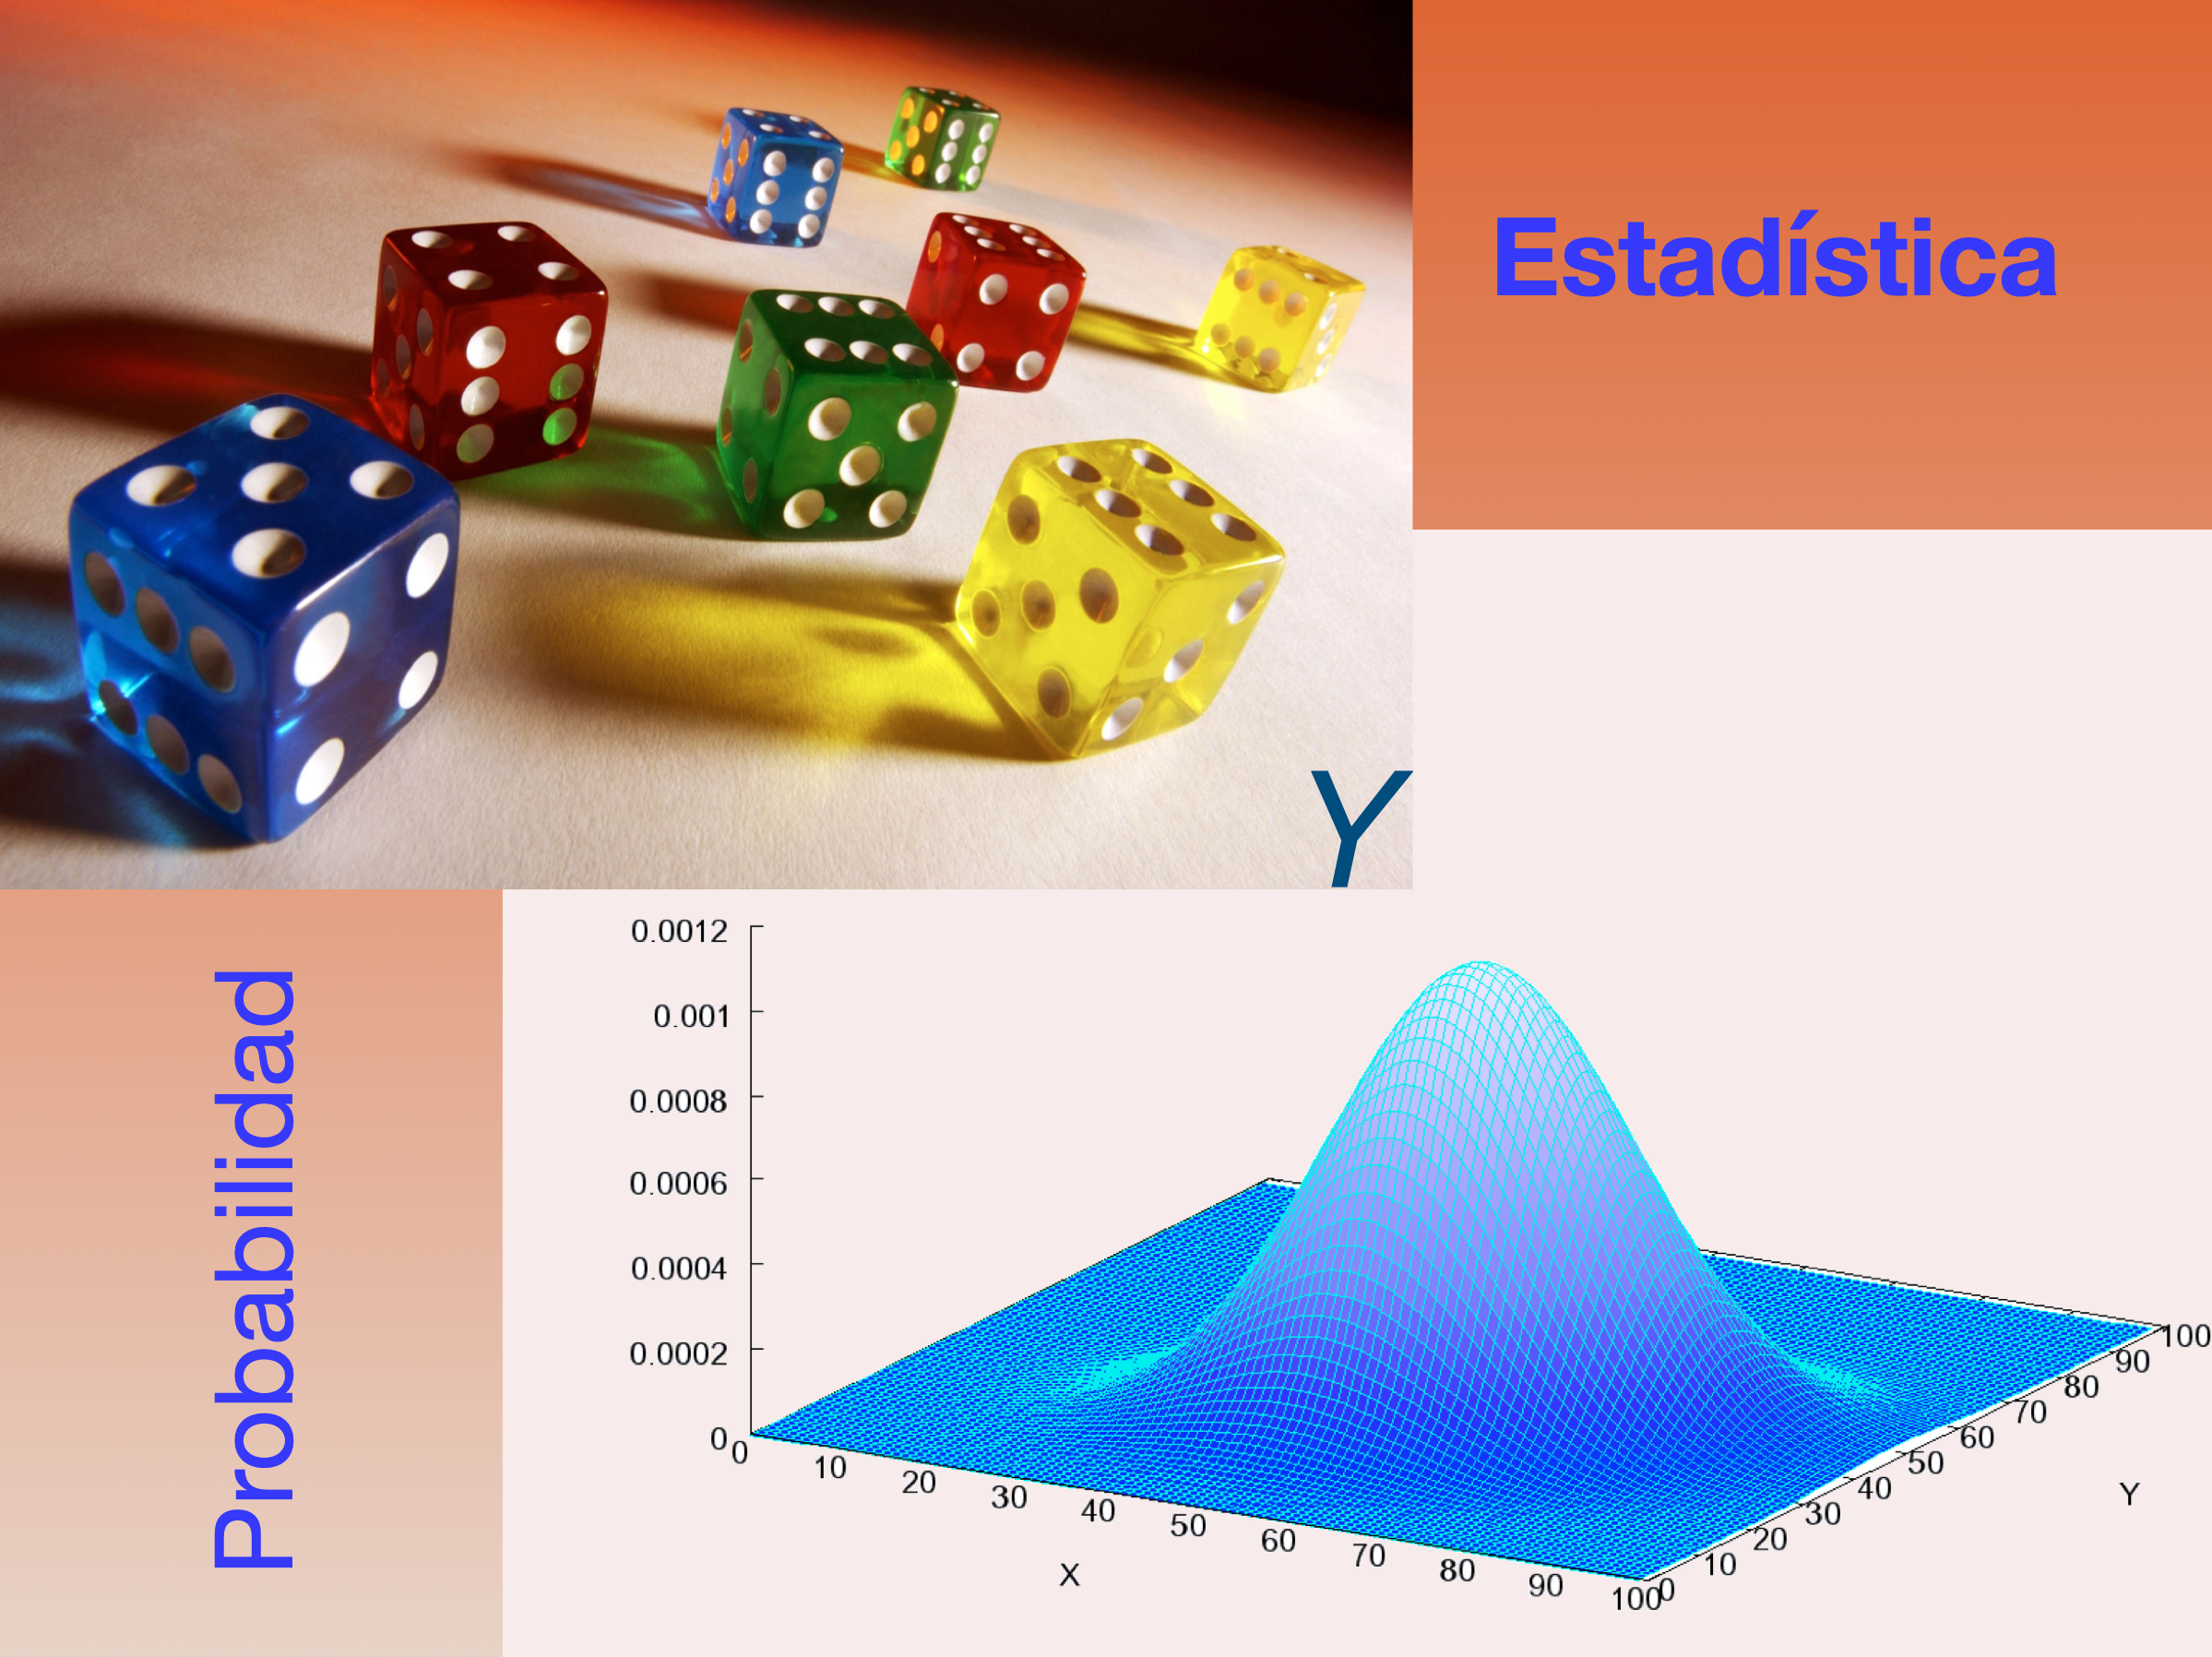
\includegraphics[width=1\textwidth]{imagenes/imagenes00/T01IM01.png}
\end{figure}

\vspace{2 cm}

\begin{quotation} \begin{quotation}
\noindent 
\begin{large}
\begin{itemize}
\item I - Estadística descriptiva
	\begin{itemize}
	\item 1 - Estadística descriptiva
	\item 2 - Distribuciones bidimensionales: Correlación y Regresión lineal
	\end{itemize}
\item II - Probabilidad
	\begin{itemize}	
	\item 3 - Cálculo de Probabilidades
	\item 4 - Distribuciones de probabilidad
	\end{itemize}
\item III - Estadística inferencial
	\begin{itemize}
	\item 5 - Distribuciones muestrales. Estimación
	\item 6 - Contraste de Hipótesis. 
	\end{itemize}
\end{itemize}
\end{large}
\end{quotation} \end{quotation}

\newpage %*****************************************************


\section{?`Qué es la Estadística?}

	\begin{tikzpicture}
	\fill [left color=black!30, right color=white] (0,0) rectangle (11.5,.1);
	\end{tikzpicture}

Podemos decir que la Estadística es la \emph{herramienta} que se utiliza cuando se quiere estudiar un hecho, el que sea, y no se conocen las leyes que lo rigen. 

En estos casos lo único que se puede hacer es \emph{observar el fenómeno} o suceso de interés y \emph{tomar datos}, y luego analizar esos datos y ver si tienen relación con otras variables, si se comportan de alguna forma especial... 

La Estadística consiste en todo eso, recoger los datos, estudiarlos, analizarlos y sacar conclusiones. Y basándonos en las observaciones, a veces seremos capaces de proponer una ley que explique o que al menos describa el comportamiento del suceso. 

Como herramienta al servicio de otras ciencias la Estadística aparece en todas partes, Física, Química, Biología... y también ciencias sociales, Economía, Sociología, Psicología...  Hasta en Lingüística se usa la estadística para determinar, por ejemplo, las letras más frecuentes en los textos de una lengua.  

\textbf{Un poco de historia...} 

Las antiguas civilizaciones, como la egipcia, la china y la azteca, ya hacían estadísticas sobre el número de personas que vivían en las ciudades, normalmente para organizar el pago de impuestos y el ejército. En general a lo largo de toda la historia los gobiernos y dirigentes de las distintas naciones han procurado disponer de datos sobre la población con fines organizativos. 

La Estadística como ciencia experimentó un gran avance gracias al desarrollo de la Matemáticas, en especial de la \emph{Teoría de la Probabilidad}, cuyas bases no fueron establecidas hasta el siglo XVII por los matemáticos franceses Pierre de \emph{Fermat} y Blaise \emph{Pascal}. ¿`Y qué tiene que ver la Probabilidad con la Estadística? ¡`Mucho! Hemos dicho que la Estadística es un instrumento para el estudio de un fenómeno cuando no se conocen que leyes lo rigen, y si hay fenómenos que no están regidos por leyes eso son los fenómenos aleatorios. Y la base matemática para el estudio estadístico de los fenómenos aleatorios la proporciona la Teoría de la Probabilidad. 

\begin{footnotesize}
\begin{quotation}
	\textcolor{gris}{INSTITUTOS NACIONAL DE ESTADÍSTICA. \textsf{INE}}
	
	\textcolor{gris}{https://www.ine.es/explica/explica.htm}
	
\end{quotation}
\end{footnotesize}

\begin{multicols}{2}
\begin{figure}[H]
	\centering
	
\includegraphics[width=.3\textwidth]{imagenes/imagenes00/T01IM03.png}
\end{figure}
\begin{figure}[H]
	\centering
	
\includegraphics[width=.3\textwidth]{imagenes/imagenes00/T01IM02.png}
\end{figure}
\end{multicols}

La estadística se divide en dos partes, la \emph{Estadística Descriptiva} que se encarga de la recogida de datos de un proceso aleatorio, clasificarlos, representarlos gráficamente y reducirlos a números estadísticos y la \emph{Estadística Inferencial} que se encarga de deducir consecuencias a partir de los datos proporcionados por la estadística descriptica y hacer predicciones. Para ello se basa en la \emph{Teoría de las probabilidades}.


\section{Estructura de este libro}




 
La estructura del libro se presenta del siguiente modo:

\vspace{5mm} %***************************
\begin{definition}
. De esta manera aparecerán las definiciones.

%\textbackslash begin\{definition\}.....\textbackslash end\{definition\}	
\end{definition}

\vspace{5mm} %***************************
\begin{theorem}
. En estos recuadros aparecerá la teoría: teoremas, propiedades, ...

%\textbackslash begin\{theoreme\} ..... \textbackslash end\{theoreme\}	
\end{theorem}

\vspace{5mm} %***************************
\begin{example}
.	Estos recuadros están reservados a los ejemplos que ilustran los distintos apartados.

%\textbackslash begin\{example\}.......\textbackslash end\{example\}	
\end{example}


\vspace{5mm} %***************************
\begin{myalertblock}{Ampliación}
	Aquí aparecerán las ampliaciones de la teoría.
\end{myalertblock}


\vspace{5mm} %***************************
\begin{myexampleblock}{Curiosidades}
	Reservamos este cuadro para     las curiosidades relacionadas con el tema que se esté tratando.
\end{myexampleblock}


\vspace{5mm} %***************************
\begin{myblock}{Resumenes}
	Al final de cada tema aparece un. resumen del mismo.
\end{myblock}


\vspace{5mm} %***************************
\begin{ejemplo}
\begin{ejre}
	Así pondremos los ejercicios del tema.
	
%\textbackslash begin\{ejemplo\} \textbackslash begin\{ejre\} .........   \textbackslash end\{ejre\} \textbackslash end\{ejemplo\}
\end{ejre}
Las soluciones a los ejercicios del tema aparecerán fuera del recuadro (dentro de ellos en los que he llamado `ejercicios resueltos').
\end{ejemplo}

Los ejercicios propuestos con solución que acompañan a todos los temas aparecen sin ningún tipo de resalte.

\vspace{5mm} %***************************
\begin{destacado}
Párrafo destacado: reservamos esta forma de resaltar para hacer incapié sobre determinados aspectos importantes del tema.

%\textbackslash begin\{destacado\}	........ \textbackslash end\{destacado\}	
\end{destacado}


\section{Guía de lectura}

\textbf{Tema 1. Estadística descriptiva unidimensional}

\begin{adjustwidth}{50pt}{25pt}
En este capítulo se explican los conceptos básicos de la estadística descriptiva: tablas, gráficos y parámetros estadísticos: de centralización, de posición, de dispersión y de forma.

Para finalizar, se presenta el coeficiente de variación de Pearson para la comparación entre distribuciones estadísticas distintas. Se introduce el concepto de  ``tipificación de la variable''.
\end{adjustwidth}

\textbf{Tema 2. Distribuciones bidimensionales. Correlación y regresión lineal}

\begin{adjustwidth}{50pt}{25pt}
En el tema se estudia la correlación lineal entre dos variables estadísticas y, en su caso (que así lo indique el diagrama de dispersión y que el coeficiente de correlación sea, en valor absoluto, próximo a la unidad), encontrar la recta que mejor se ajusta a la nube de puntos, la recta de regresión.

Se hacen predicciones con las dos rectas de regresión haciendo hincapié en que la mayor fiabilidad de las interpolaciones.

Se menciona la recta de Tukey como alternativa a la de regresión ante la presencia de \emph{outliers} y, como ampliación, se habla de las correlaciones exponencial y potencial, ambas no lineales.
\end{adjustwidth}

\textbf{Tema 3. Probabilidad}

\begin{adjustwidth}{50pt}{25pt}
Después de introducida el álgebra de los sucesos de experimentos aleatorio se dan varias definiciones de probabilidad: a posteriori o frecuencialista y a priori o regla de Laplace. A continuación se enuncia la definición axiomática de Kolmogorov.

Seguimos com la definición de probabilidad condicionada y los teoremas de la probabilidad total y de Bayes. Este tema, por su interés y dificultad, se ve con más detenimiento y se acompaña de gran cantidad de ejemplos y ejercicios resueltos y propuestos con solución.
\end{adjustwidth}

\textbf{Tema 4. Distribuciones de probabilidad}

\begin{adjustwidth}{50pt}{25pt}
Las distribuciones de probabilidad son idealizaciones matemáticas de las distribuciones estadísticas. En el presente tema se analizan detalladamente las distribuciones de probabilidad más importantes: la binomial (para variable aleatoria discreta) y la normal (para variable aleatoria continua).

Como distribuciones de variable aleatoria discreta se analizan también la distribución uniforme, la de Bernouilli y la de Poisson. Para variable continua se estudian, someramente, la distribución uniforme continua y la exponencial.

En la distribución normal se estudi el uso de tablas para la normal típica o standard N(0,1) y la ``tipificación de la variable'' para cualquier distribución normal $N(\mu,\sigma)$.

El tema termina con el estudio de la aproximación de la binomial por la normal y la correspondiente ``corrección por continuidad''.

Este tema se acompaña de gran cantidad de ejemplos y ejercicios resueltos y propuestos con solución.

\end{adjustwidth}

\textbf{Tema 5. Distribuciones muestrales. Estimación}

\begin{adjustwidth}{50pt}{25pt}
Comenzamos con la definición y cálculo de los intervalos característicos en una distribución normal típica y en una normal cualquiera, que usaremos más tarde en la estimación de parámetros por intervalos.

Estudiamos la distribución de las medias muestrales y analizamos el teorema central del límite. Se aprende a hacer estimaciones puntuales y por intervalos de confianza de la media de la población (conocida una muestra) y de la media de una muestra (conocida la población). Se hace notar la relación entre el nivel de confianza, el error máximo admisible y el tamaño de la muestra.

Como ampliación, vemos la distribución de la diferencia de medias de dos muestras.

El tema acaba analizando la distribución de la proporción y haciendo estimaciones para la proporción de una población y de una muestra.

Este tema se acompaña de gran cantidad de ejemplos y ejercicios resueltos y propuestos con solución.
\end{adjustwidth}

\textbf{Tema 6. Contraste de hipótesis}

\begin{adjustwidth}{50pt}{25pt}

En el estudio del contraste de hipótesis se estudian los elementos que la componen así como la metodología general de su aplicación, teniendo en cuenta los dos tipos de posibles errores en que se puede caer.

Estudiamos el contraste de hipótesis para la media de un población y para la proporción de una población. Como ampliación, vemos el contraste de hipótesis para la diferencia de medias de dos poblaciones.

Este tema se acompaña de gran cantidad de ejemplos y ejercicios resueltos y propuestos con solución.
\end{adjustwidth}

\textbf{Apéndices}

\begin{adjustwidth}{50pt}{25pt}
A - ``Ideas básicas de la teoría de conjuntos'': analizamos el álgebra de Boole como sistema lógico de amplia aplicación en probabilidad.

B - ``Combinatoria. Técnicas de conteo'': principio de multiplicación, principio del palomar, permutaciones, variaciones y combinaciones 8con y sin repetición). Estrategia de los diagramas de árbol. Números combinatorios, triangulo de Tartaglia y binomio de Newton.

C - ``Tablas de las distribuciones Binomial y Normal''.

D - ``El problema del borracho''. Analizamos en este apéndice el famoso problema cuyo enunciado dice: \emph{
``Un borracho parte de un farol dando pasos de igual longitud hacia ambos lados. ?`Cuál es la probabilidad de que después de $N$ pasos vuelva al farol?''
}
\end{adjustwidth}






\section{Acerca de este libro}

El presente libros, colección de apuntes, contempla la parte de estadística de los temarios de bachillerato. Junto a los otros dos, ``Cálculo infinitesimal (avanzado) para bachillerato'' y ``Álgebra lineal y geometría (avanzadas) para bachillerato'', este ``Probabilidad y estadística (avanzadas) para bachillerato'' contemplan todo el temario actual de matemáticas de este nivel de enseñanza.

Es cierto que falta la parte de ``Programación lineal'' que haré en una nueva pequeña entrega.

La confección de estos textos es fruto de una larga experiencia como profesor de matemáticas de secundaria y para ello me he basado en mis más de treinta años de docencia  y en la de tantos autores que han contribuido a la explicación de estos conceptos a multitud de alumnos. He usado también apuntes y problemas de libros de texto de segundo de bachillerato así como apuntes y ejercicios encontrados en la web y pruebas de acceso a la universidad de distintas comunidades autónomas. Gracias a todos sus autores por su inestimable ayuda para la confección de estos textos que espero que sirva a alguien y que escribo libre de todo tipo de derechos. 


\vspace{5mm}
\centering{
\fcolorbox{black}{fondoblau}{
\parbox{0.95\textwidth}{
	\textit{Este material es un conjunto de apuntes personales que comparto gratuitamente en la red. Se agradecería la comunicación de la detección de cualquier error.}
}}}
\justify

\emph{Este documento se comparte bajo licencia `Attribution-NonCommercial 4.0 International (CC BY-NC 4.0)'}


\begin{multicols}{2}
\begin{figure}[H]
	\centering
	
\includegraphics[width=.4
	\textwidth]{imagenes/imagenes00/licencia.png}
\end{figure}
\begin{figure}[H]
	\centering
	
\includegraphics[width=.3
	\textwidth]{imagenes/firma.png}
\end{figure}
\end{multicols}






\part[Estadística Descriptiva]{Estadística Descriptiva\\[7ex]\makebox[0pt]{
\includegraphics[width=1\textwidth]{imagenes/part1.png}}}

\chapter{Estadística Descriptiva unidimensional}
\label{estad-descrip}
\vspace{-5 mm} %****************************************
\begin{tikzpicture}
	\fill [left color=red!50, right color=teal!50] (0,0) rectangle (6.5,.1);
	\fill [left color=teal!50, right color=green!50] (6.5,0) rectangle (11.5,.1);
	\end{tikzpicture}
	
\section{Terminología}

\begin{definition}
.	

\begin{itemize}
	\item \textbf{Población}
	
	\hspace {1cm} Conjunto sobre el que se va a realizar es estudio estadístico.
	
	\item \textbf{Muestra}
	
	\hspace {1 cm} Cualquier subconjunto de la población.	
	
	\item \textbf{Individuo}
	
	\hspace {1 cm} Cualquier elemento de la población.
	
	\item \textbf{Serie o distribición estadística}
	
	\hspace {1 cm} Conjunto de datos (cuantitativos o cualitativos) que se obtienen al estudiar un \emph{carácter} de los individuos de una población o muestra.
	
	\item \textbf{Carácter estadístico} 
	
	\hspace {1 cm} Propiedad o característica de los individuos que se desea someter a estudio.
	
	\underline{Tipos de caracteres estadísticos}:
	
	\begin{itemize}
	\item \textbf{Cualitativos o \emph{Atributos.}} (Sexo, Profesión, ...)
	
	\hspace{1 cm} No se pueden medir, describen \emph{modalidades}.
	
	\item \textbf{Cuantitativos o \emph{Variables.}} (Edad, Altura, ...)
	
	\hspace{1 cm} Se pueden medir, toman valores numéricos.
	\end{itemize}
	
	\underline{Tipos de variables estadísticos}:
	
	\begin{itemize}
	\item \textbf{Discretas.} (Número de hijos, Edad --en años--,...)
	
	\hspace{1 cm} Toman valores aislados.
	
	\item \textbf{Continuas.} (Altura de personas, Peso, ...)
	
	\hspace{1 cm} Pueden tomar cualquier valor en un intervalo.
	\end{itemize}
	
\end{itemize}
\end{definition}

\section{Frecuencias}
	
\begin{definition} .
	Dada una serie estadística que contenga $N$ datos, llamaremos:
	
	\begin{itemize}
	\item \textbf{Frecuencia absoluta}	de un dato, al número de veces que aparece ese dato en la serie. $\ \boldsymbol{n_i}$
	\item \textbf{Frecuencia relativa} de una dato, al cociente entre la frecuencia absoluta del mismo y el número total de datos de la serie. $\ \boldsymbol{f_i=n_i/N}$
	\vspace{1 cm}
	
	\emph{``Supuesta la variable estadística \textbf{ordenada} de mayor a menor'', se definen:}
	
	\item \textbf{Frecuencia absoluta acumulada} del dato que ocupa el lugar $k$-ésimo en la serie, $x_k$,  es el valor que se obtiene sumando todas las frecuencias absolutas de los datos anteriores hasta llegar al $x_k$:
	
	$\boldsymbol{N_i}=\displaystyle \sum_{i=1}^k n_i=n_1+n_2+ \cdots + n_k$
	
	\item \textbf{Frecuencia absoluta relativa} del dato $x_k$ es el valor que se obtiene sumando todas las frecuencias relativas hasta llegar al valor $x_k$:
	
	$\boldsymbol{F_i=\displaystyle \sum_{i=1}^k f_i=f_1+f_2+ \cdots + f_k=}$
	
	\hspace {1 cm} \textcolor{gris}{$= \dfrac{n_1+n_2+\cdots +n_k}{N}=\dfrac{n_k}N$}
	\end{itemize}
\end{definition}

\vspace{5mm}%**********************
\begin{theorem} .
	$$ \displaystyle \sum_{i=1}^N n_i=N; \hspace{2cm} \sum_{i=1}^N fi=1$$
	
	$$N_N=N; \ \ F_N=1;\ \ 0\le n_1\le N; \ \ 0\le f_i\le 1; \ \ N_i=N_{i-1}+n_i$$
\end{theorem}

Para facilitar la lectura de los datos estadísticos, éstos se suelen agrupar y presentar en forma de \subrayado{\emph{\textbf{Tablas de Frecuencias}}}:

\begin{table}[H]
\centering
\begin{tabular}{|c|c|c|c|c|}
\hline
Valores  & \multicolumn{4}{c|}{Frecuencias}                                  \\ \cline{2-5} 
de la    & \multicolumn{2}{c|}{Ordinarias} & \multicolumn{2}{c|}{Acumuladas} \\ \cline{2-5} 
Variable & $n_i$  & $f_i$    & $N_i$    & $F_i$  \\ \hline
$x_i$  & (absoluta)   & (relativa)  & (absoluta)  & (relativa) \\
  &  &  &  &     
\end{tabular}
\end{table}


\begin{example} .
	Una empresa se propone reestructurar las remuneraciones de sus trabajadores, se estudia los años de éstos determinándose los siguientes resultados: 
	
	\begin{center}
	4 - 5 - 4 - 6 - 7 - 9 - 7 - 7 - 5 - 8 - 8 - 7 - 6 - 7 - 7 
	
	4 - 6 - 8 - 8 - 9 - 6 - 8 - 9 - 5 - 6 - 5 - 4 - 7 - 9 - 6  
	
	7 - 6 - 5 - 4 - 4 - 4 - 6 - 8 - 8 - 7 - 8 - 9 - 5 - 5 - 4 
	
	6 - 7 - 9 - 5 - 4 \end{center}
	
	Agrupamos y ordenamos decrecientemente los 50 valores.
	
	\begin{table}[H]
	\centering
	\begin{tabular}{c|r|rrr}
	\textbf{Años de servicio} & $n_i$       & \multicolumn{1}{r|}{$f_i$} & \multicolumn{1}{r|}{$N_i$}       & $F_i$         \\ \hline
	4                         & 9           & \multicolumn{1}{r|}{0.18}  & \multicolumn{1}{r|}{9}           & 0.18          \\
	5                         & 8           & \multicolumn{1}{r|}{0.16}  & \multicolumn{1}{r|}{17}          & 0.34          \\
	6                         & 9           & \multicolumn{1}{r|}{0.18}  & \multicolumn{1}{r|}{26}          & 0.52          \\
	7                         & 10          & \multicolumn{1}{r|}{0.20}  & \multicolumn{1}{r|}{36}          & 0.72          \\
	8                         & 8           & \multicolumn{1}{r|}{0.16}  & \multicolumn{1}{r|}{44}          & 0.88          \\
	9                         & 6           & \multicolumn{1}{r|}{0.12}   & \multicolumn{1}{r|}{\textbf{50}} & \textbf{1.00} \\ \cline{1-3}
	Totales                   & \textbf{50} & \textbf{1.00}              &                                  &              
	\end{tabular}
	\end{table}
\end{example}

\subsection{Frecuencias para datos agrupados}

Si la variable es continua o el número de datos es muy grande, estos se \emph{agrupan en intervalos} llamados \textbf{\emph{`clases'}}. En general se toman intervalos de la misma amplitud y cerrados por la izquierda y abiertos por la derecha:

$[a,b_1[,\ [b_1,b_2[,\ \cdots ,\ [b_{k-1},b_k[,\ \cdots ,\ [b_N,b[$

\vspace{5mm}%**********************
\begin{definition}.
		Se llama \textbf{marca de clase} al punto medio de cada intervalo:
		
		Para el intervalo $\ [b_{k-1},b_k[\ $, su marca de clase es $\ m_k=\dfrac{b_{k-1}+b_k}{2}\ $.
		
		\vspace{2mm} Este valor representará a todos los datos que estén en su interior.
		
		\vspace{2mm} Es evidente que al agrupar datos en intervalos \emph{se pierde información} ya que se supone que los datos se distribuyen homogéneamente alrededor de la marca de clase y esto no siempre es cierto.
\end{definition}

Para el número de intervalos y forma de agrupamiento de los datos hay muchos criterios diferentes, entre ellos mostramos los que aparecen en la siguiente figura:


		\begin{figure}[H]
			\centering
			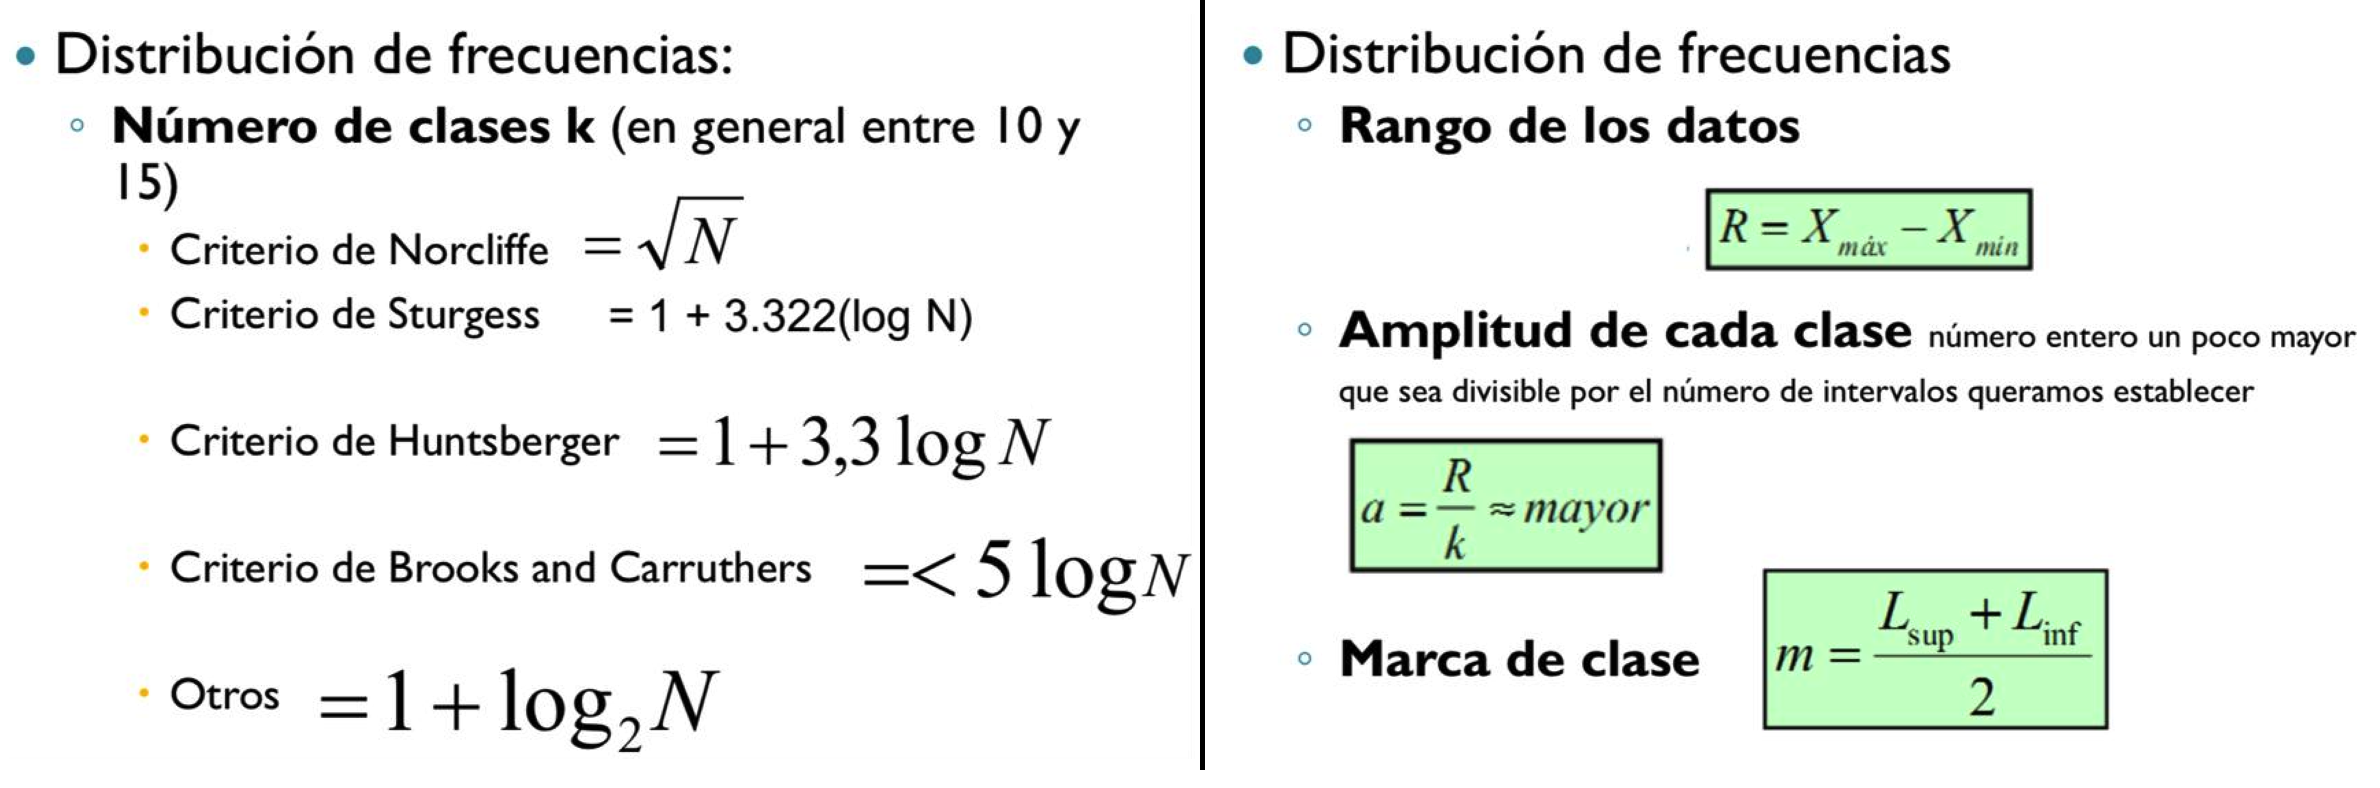
\includegraphics[width=1.05\textwidth]{imagenes/imagenes01/T01IM01.png}
		\end{figure}

Veamos un ejemplo:

\begin{example}. \label{ejparamedia}
	Las edades de un conjunto de niños son: 3, 7, 10, 10, 6, 5, 4.5, 12, 11, 10, 15, 10.5, 6, 2, 10, 9, 10, 4, 15, 13, 14, 12, 7, 10, 6, 8. Agrupando los datos, construir la tabla de frecuencias.
	
	\vspace{6mm} En los 26 datos hay 15 valores distintos (desde el 2 hasta el 15). Aplicando, p.e., el criterio de Norcliffe, tendremos que construir $\sqrt{15}\approx 4$ intervalos.
	
	\vspace{2mm}La amplitud de cada intervalo debe ser $\dfrac{15-2}{4}=\dfrac{13}{4}=3.25 \to 3.5 \text{ ó } 4$. Tomaremos $4$ como amplitud. Así, los intervalos en que agrupar los datos serán $[2,6[,\ [6,10[,\ [10,14[, \ [14,18[$
	
	\vspace{2mm}Distribuyendo, ahora, los datos en sus clases construimos la tabla de frecuencias.
	
	% Please add the following required packages to your document preamble:
% \usepackage{multirow}
\begin{table}[H]
\centering
\begin{tabular}{cr|r|rrr}
\multicolumn{1}{c|}{Edades}    & \multicolumn{1}{c|}{\multirow{2}{*}{\begin{tabular}[c]{@{}c@{}}Marcas\\ de clase\end{tabular}}} & \multicolumn{2}{c|}{Frecuencias}                        & \multicolumn{2}{c|}{F. acumuladas}                       \\ \cline{3-6} 
\multicolumn{1}{c|}{$x_i$}     & \multicolumn{1}{c|}{}                                                                             & \multicolumn{1}{c|}{$n_i$} & \multicolumn{1}{c|}{$f_i$} & \multicolumn{1}{c|}{$N_i$} & \multicolumn{1}{c|}{$F_i$}  \\ \hline
\multicolumn{1}{c|}{$[2,6[$}   & 4                                                                                                 & 5                          & \multicolumn{1}{r|}{5/26}  & \multicolumn{1}{r|}{5}     & \multicolumn{1}{r|}{5/26}  \\
\multicolumn{1}{c|}{$[6,10[$}  & 8                                                                                                 & 7                          & \multicolumn{1}{r|}{7/26}  & \multicolumn{1}{r|}{12}    & \multicolumn{1}{r|}{12/26} \\
\multicolumn{1}{c|}{$[10,14[$} & 12                                                                                                & 11                         & \multicolumn{1}{r|}{11/26} & \multicolumn{1}{r|}{23}    & \multicolumn{1}{r|}{23/26} \\
\multicolumn{1}{c|}{$[14,18[$} & 16                                                                                                & 3                          & \multicolumn{1}{r|}{3/26}  & \multicolumn{1}{r|}{26}    & \multicolumn{1}{r|}{26/26} \\ \cline{3-3}
                               &                                                                                                   & N=26                       &                            &                            &                            \\ \cline{3-3}
\end{tabular}
\end{table}
\end{example}

\textbf{Intervalos no solapados:} si los datos ya aparecen agrupados pero lo están en intervalos no solapados se tomarán intervalos que contengan a estos pero sin modificar las frecuencias.

Lo vemos con un ejemplo:

\begin{example}.
	% Please add the following required packages to your document preamble:
% \usepackage{multirow}
\begin{table}[H]
\centering
\begin{tabular}{c|ccc|c}
Internavo & $n_i$ & \multirow{5}{*}{$\quad \Rightarrow \quad$} & Intervalo   & $n_i$ \\ \cline{1-2} \cline{4-5} 
10 a 19   & 10    &                                            & [9.5,19.5[  & 10    \\
20 a 29   & 15    &                                            & [19.5,29,5[ & 15    \\
30 a 39   & 17    &                                            & [29.5,39,5[ & 17    \\
39 a 49   & 11    &                                            & [39.5,49.5[ & 17   
\end{tabular}
\end{table}
\end{example}

\section{Representaciones gráficas}


En los análisis estadísticos, es frecuente utilizar representaciones visuales complementarias de las tablas que resumen los datos de estudio. Con estas representaciones, adaptadas en cada caso a la finalidad informativa que se persigue, se transmiten los resultados de los análisis de forma rápida, directa y comprensible.

Cuando se muestran los datos estadísticos a través de representaciones gráficas, se ha de adaptar el contenido a la información visual que se pretende transmitir. Para ello, se barajan múltiples formas de representación. Los tipos más frecuentes de representaciones estadísticas son:

\begin{itemize}
	\item \textbf{Diagramas de barra}s: muestran los valores de las frecuencias absolutas sobre un sistema de ejes cartesianos, cuando el carácter estadístico en estudio es un atributos o  una variable discreta.
	\item \textbf{Histogramas}: formas especiales de diagramas de barras para distribuciones de variable continua.
	\item \textbf{Polígonos de frecuencias}: formados por líneas poligonales abiertas sobre un sistema de ejes cartesianos.
	\item \textbf{Gráficos de sectores}: circulares o de tarta, dividen un círculo en porciones proporcionales según el valor de las frecuencias relativas. \textcolor{gris}{Este tipo de diagramas no es nada recomendado.\footnote{Lo veremos más adelante, en su apartado correspondiente.}}
	\item \textbf{Pictogramas}: o representaciones visuales figurativas. En realidad son diagramas de barras en los que las barras se sustituyen con dibujos alusivos a la variable. 
	\item \textbf{Cartogramas}: expresiones gráficas a modo de mapa.
	\item \textbf{Pirámides de población}: para clasificaciones de grupos de población por sexo y edad.
\end{itemize}

\subsection{Diagrama de barras}

\begin{definition}
	. Un \textbf{diagrama de barras} es una representación gráfica en un eje cartesiano de las frecuencias de una variable cualitativa (atributo) o cuantitativa discreta.
		
	\vspace{2mm} Se representan, en el eje de abcisas, los valores de la serie estadística, y en el de ordenadas, los valores de las frecuencias absolutas.
	
	\vspace{2mm} Se suelen usar para comparar magnitudes de varias categorías, ver la evolución en el tiempo de una magnitud concreta, etc.
\end{definition}

\begin{example}

		\begin{figure}[H]
			\centering
			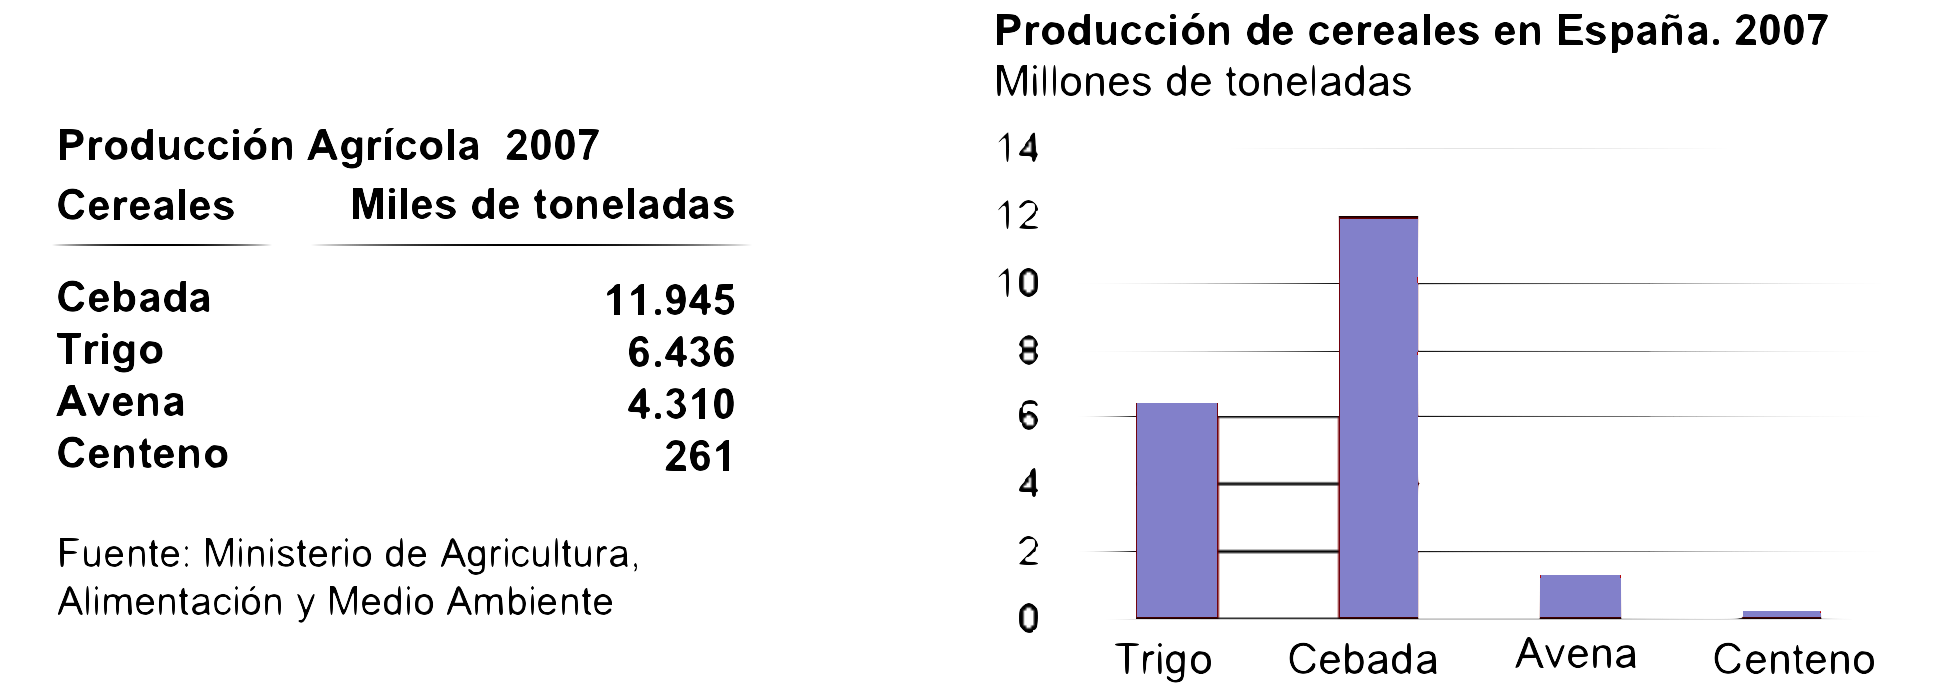
\includegraphics[width=1\textwidth]{imagenes/imagenes01/T01IM02.png}
			\caption*{\footnotesize{Diagrama de barras. (INE)}}
		\end{figure}
\end{example}

\subsection{Histogramas}
\begin{definition}
	. Los \textbf{histogramas} se usan para representar las frecuencias de una variable cuantitativa continua.

	\vspace{2mm} En uno de los ejes se posicionan las clases de la variable continua (los intervalos) y en el otro eje las frecuencias absolutas. No existe separación entre las barras.	
\end{definition}


\begin{example}

	\begin{figure}[H]
			\centering
			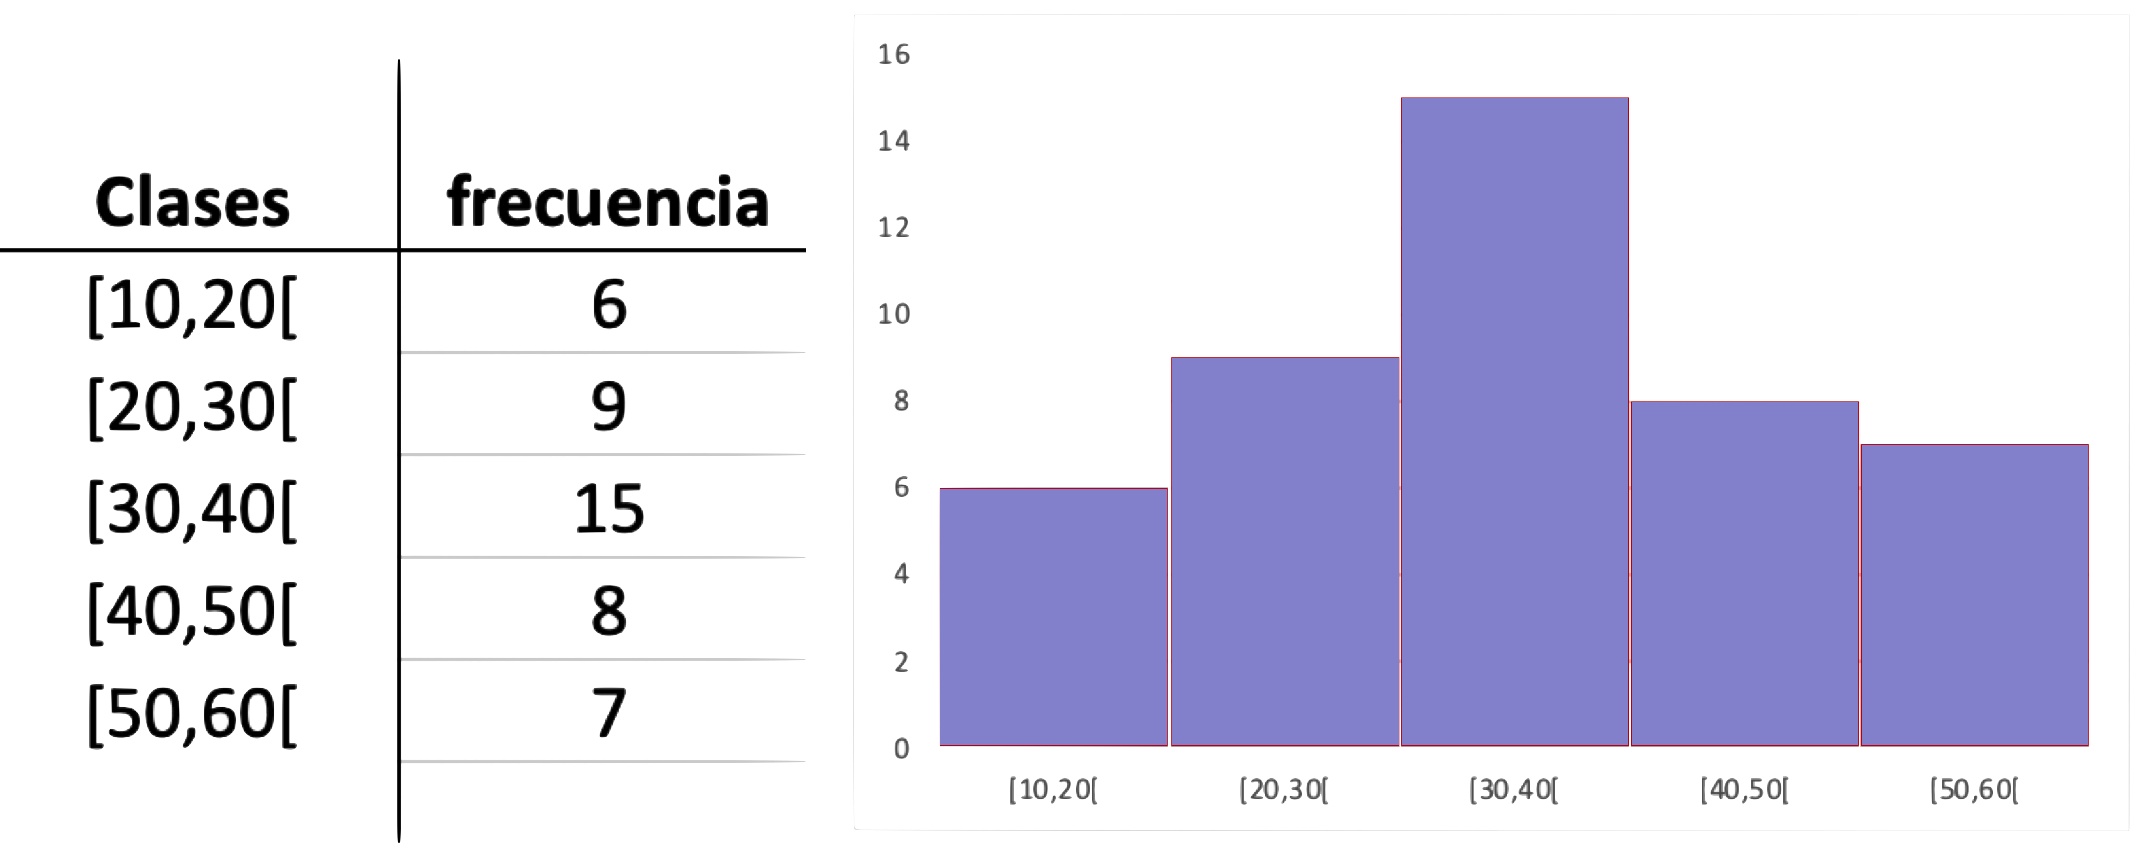
\includegraphics[width=.8\textwidth]{imagenes/imagenes01/T01IM03.png}
			\caption*{\footnotesize{Histograma.}}
		\end{figure}
\end{example}

\vspace{5mm}%**********************
\begin{example}

	Si las clases no son de la misma amplitud, no es la altura de los rectángulos sino su área el que debe ser proporcional a la frecuencia absoluta de cada una de ellas.

\begin{figure}[H]
			\centering
			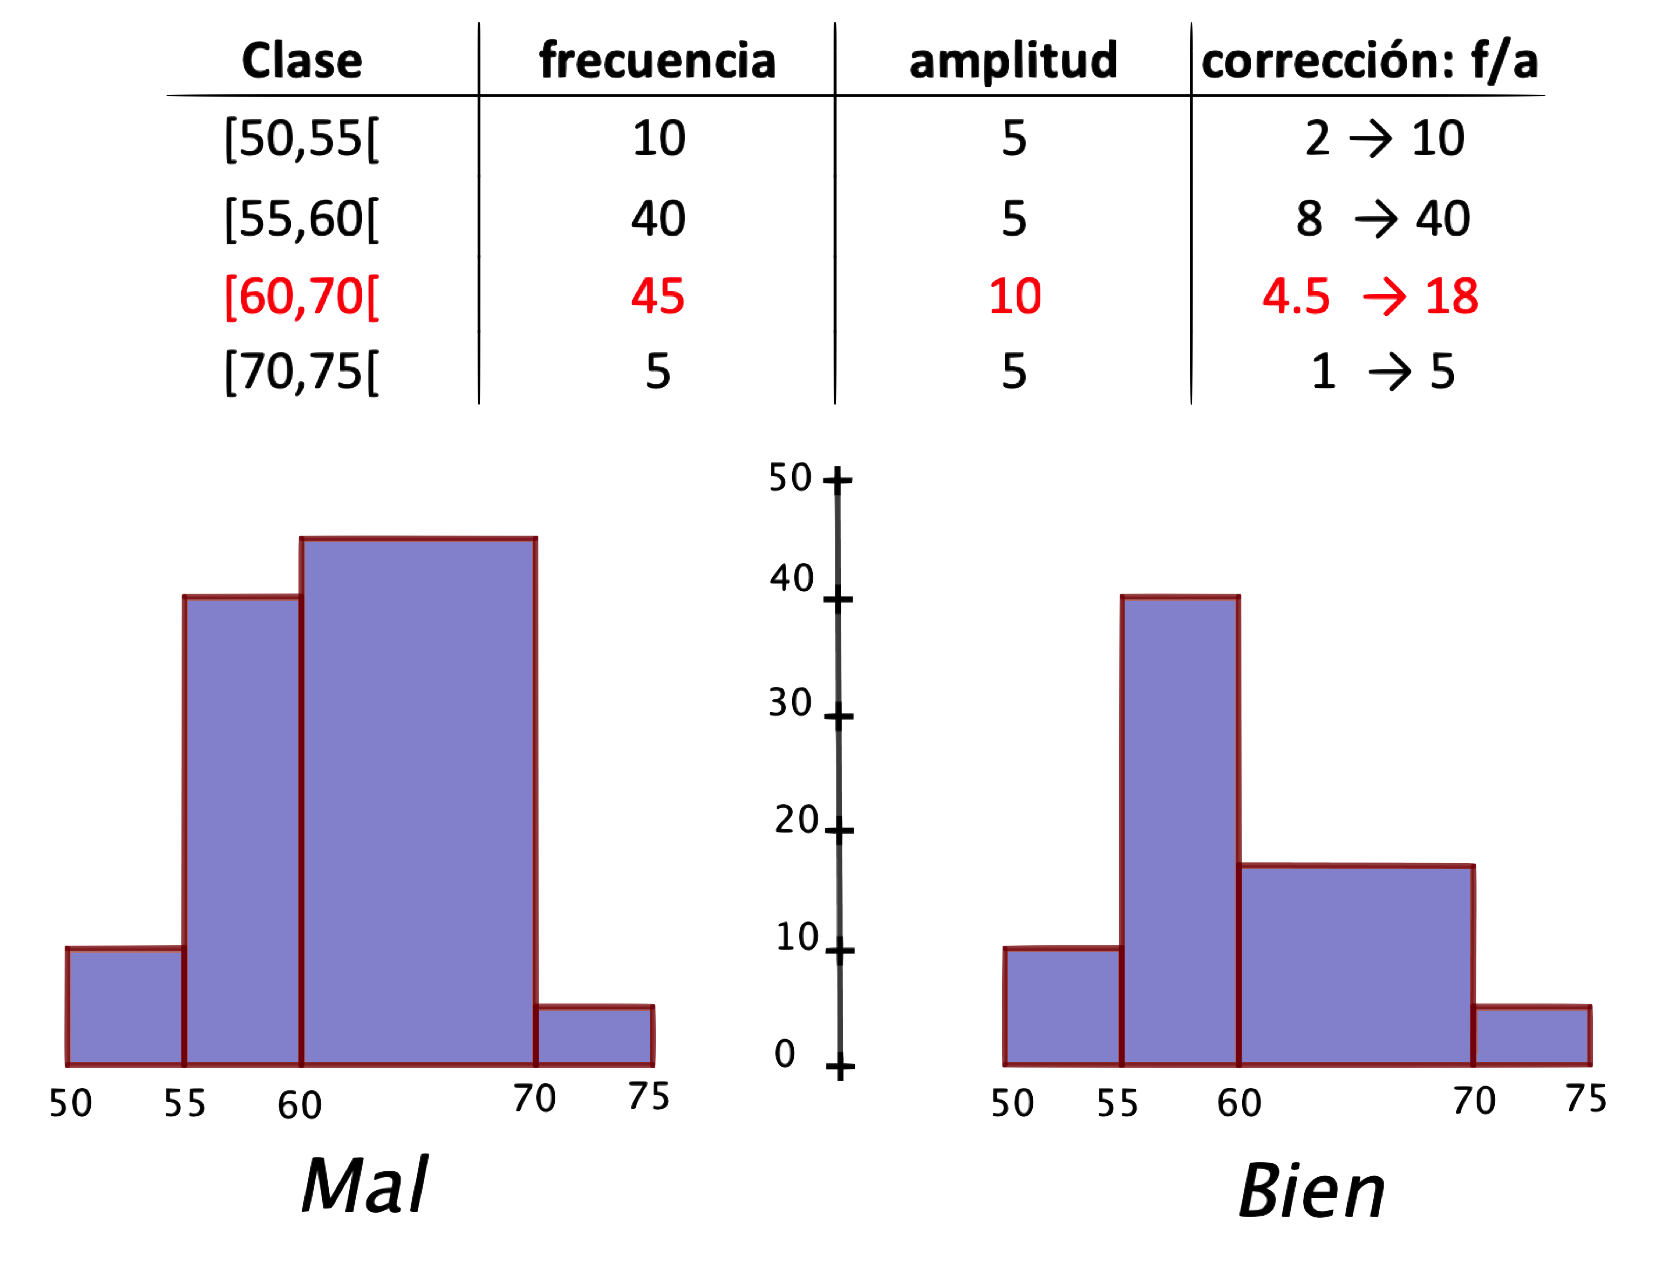
\includegraphics[width=.7\textwidth]{imagenes/imagenes01/T01IM04.png}
		\end{figure}

\end{example}



\subsection{Polígonos de frecuencias}

\begin{definition}
	. Un \textbf{polígono de frecuencias} es una linea poligonal que une o bien el extremos de las barras en un diagrama de barras o bien los puntos medios de las partes superiores de los rectángulos que forman un histograma	.
\end{definition}


\vspace{3cm} %*****************************************

\textcolor{white}{.}  %*****************************************

\vspace{3cm} %*****************************************

\begin{example}

\begin{figure}[H]
			\centering
			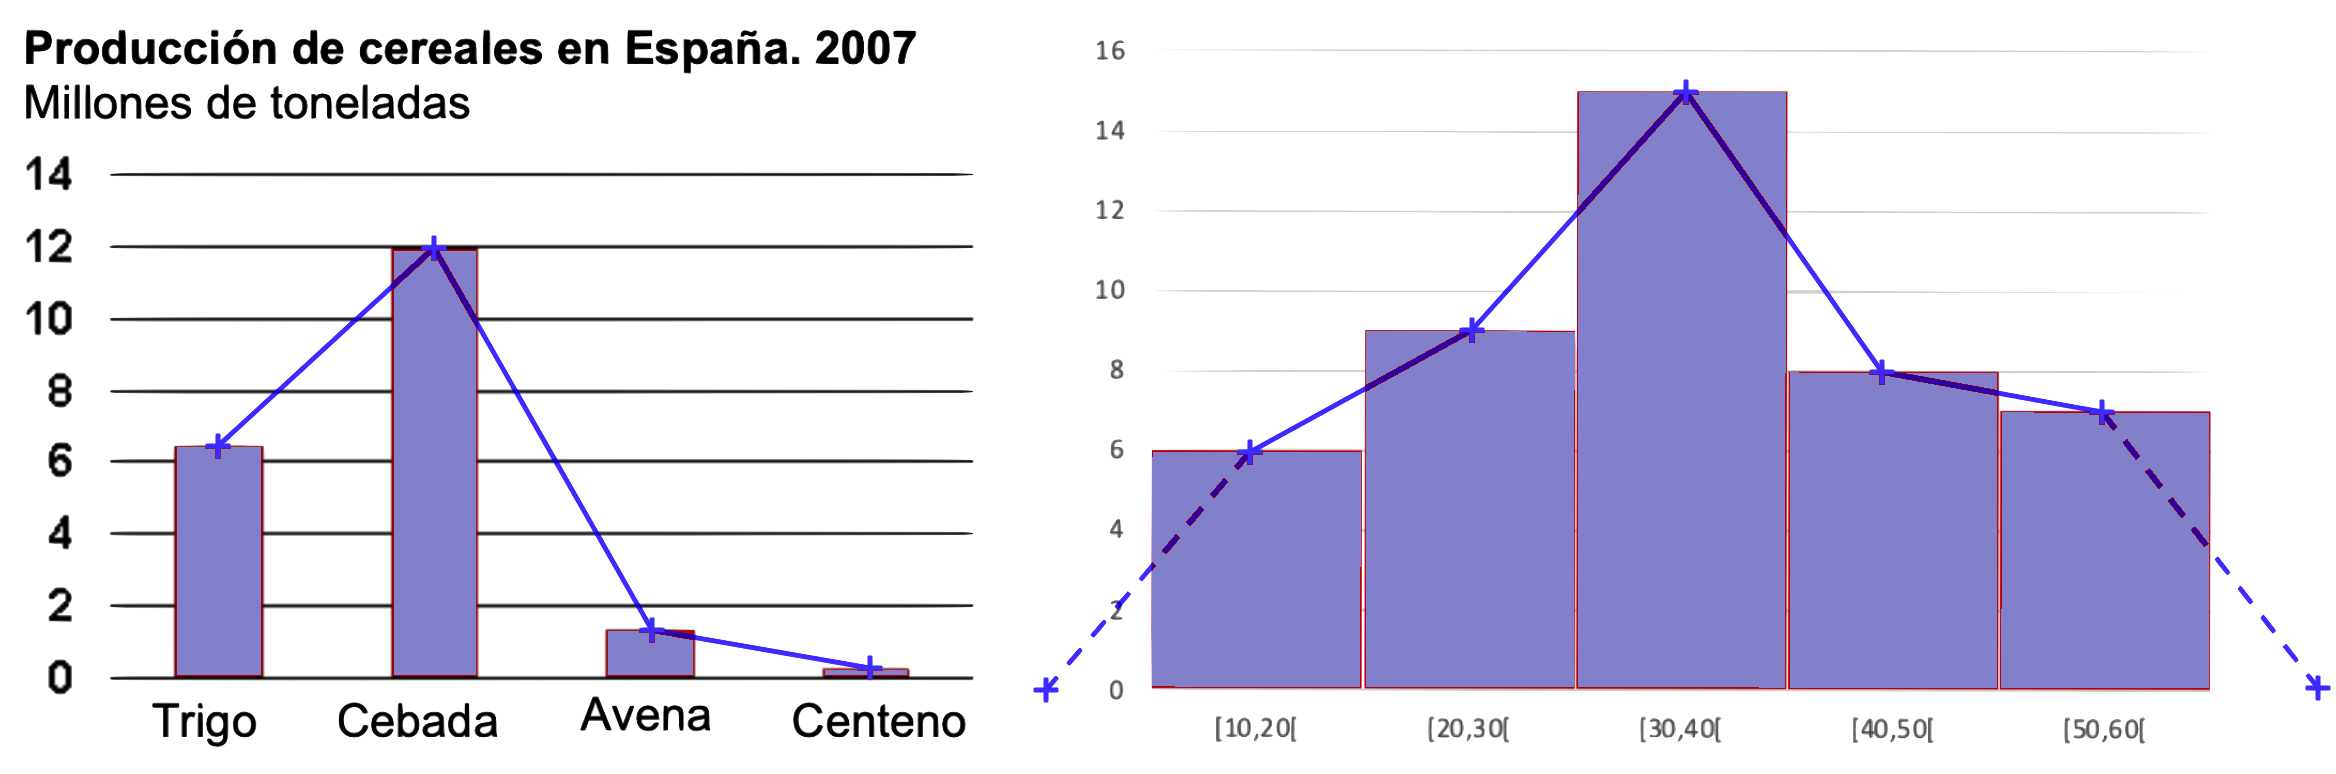
\includegraphics[width=1\textwidth]{imagenes/imagenes01/T01IM05.png}
			\caption*{\footnotesize{Polígonos de frecuencias (absolutas) en diagrama de barras y en histograma.}}
		\end{figure}


Si en lugar de usar en el eje de ordenadas las frecuencias absolutas se usan las frecuencias absolutas acumuladas, se obtienen los \emph{polígonos de frecuencias absolutas acumuladas}. También se habla de polígonos de frecuencias relativas y de frecuencias relativas acumuladas. 

El uso de este tipo de representaciones gráficas es muy útil para el cálculo aproximado de parámetros de posición, como veremos en el próximo apartado. 

\end{example}

\vspace{2cm} %*****************************************
\subsection{Diagrama de sectores}
\vspace{2cm} %*****************************************
\begin{definition}
	. En un \textbf{diagrama de sectores	},  la serie estadística se representa como sectores circulares de ángulo (área) proporcional a la frecuencia de cada dato.
	
	\vspace{2mm} Se suele usar para datos cualitativos y con pocos valores.
\end{definition}


\vspace{4cm} %*****************************************
\textbf{ \emph{``Tartas no, gracias''}}.

	\begin{figure}[H]
			\centering
			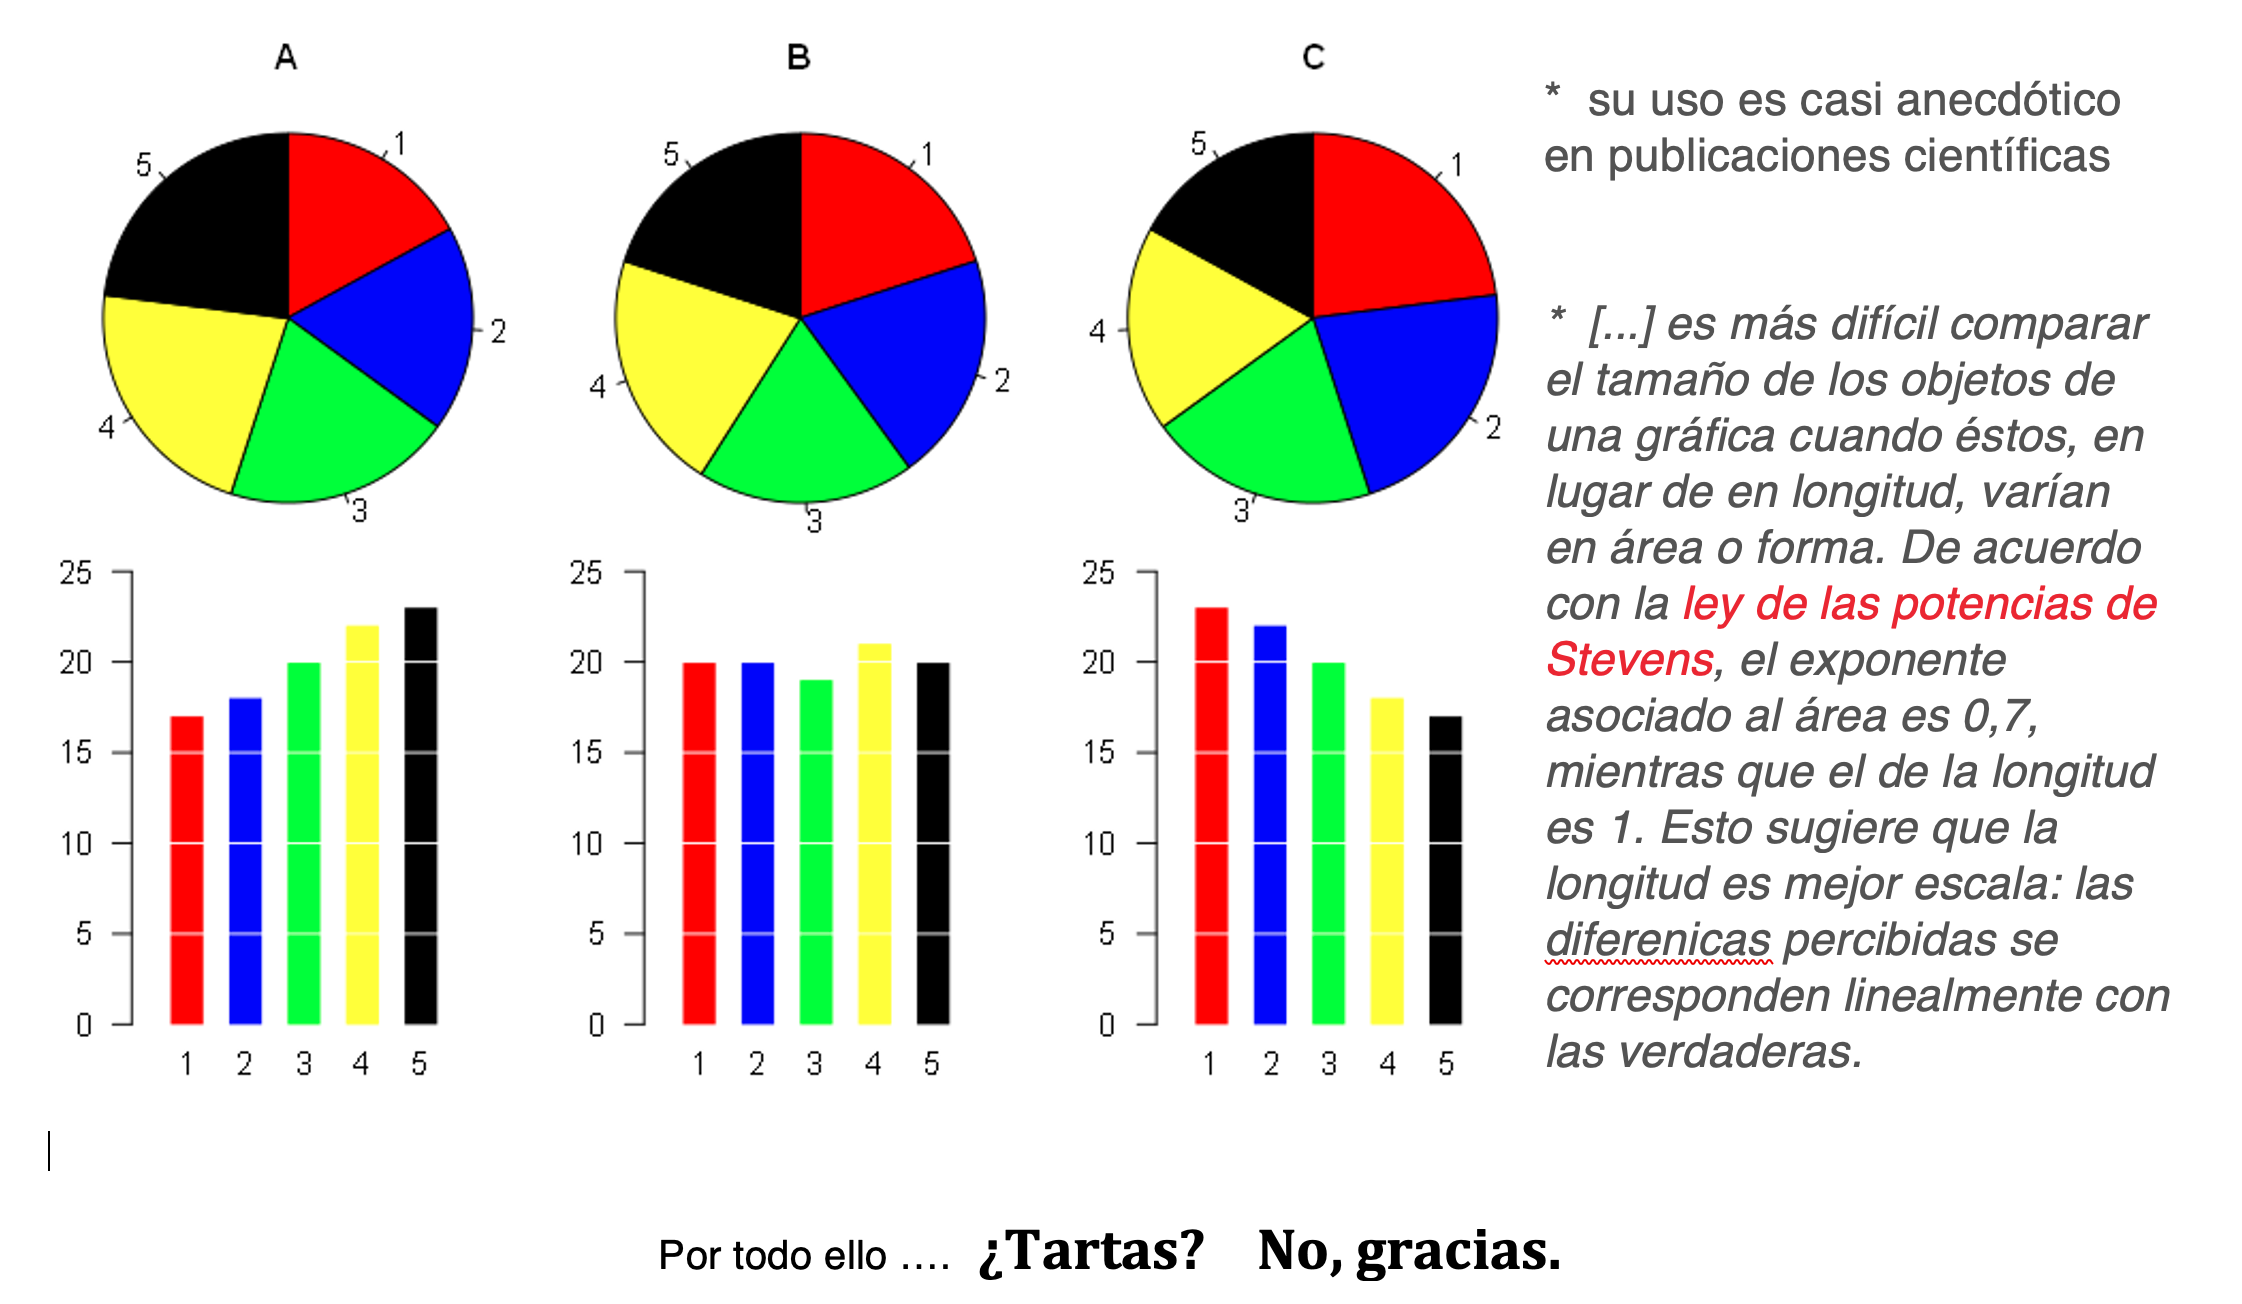
\includegraphics[width=1\textwidth]{imagenes/imagenes01/T01IM06.png}
			\caption*{\footnotesize{Los diagramas de sectores no son aconsejables.}}
		\end{figure}

	\begin{figure}[H]
			\centering
			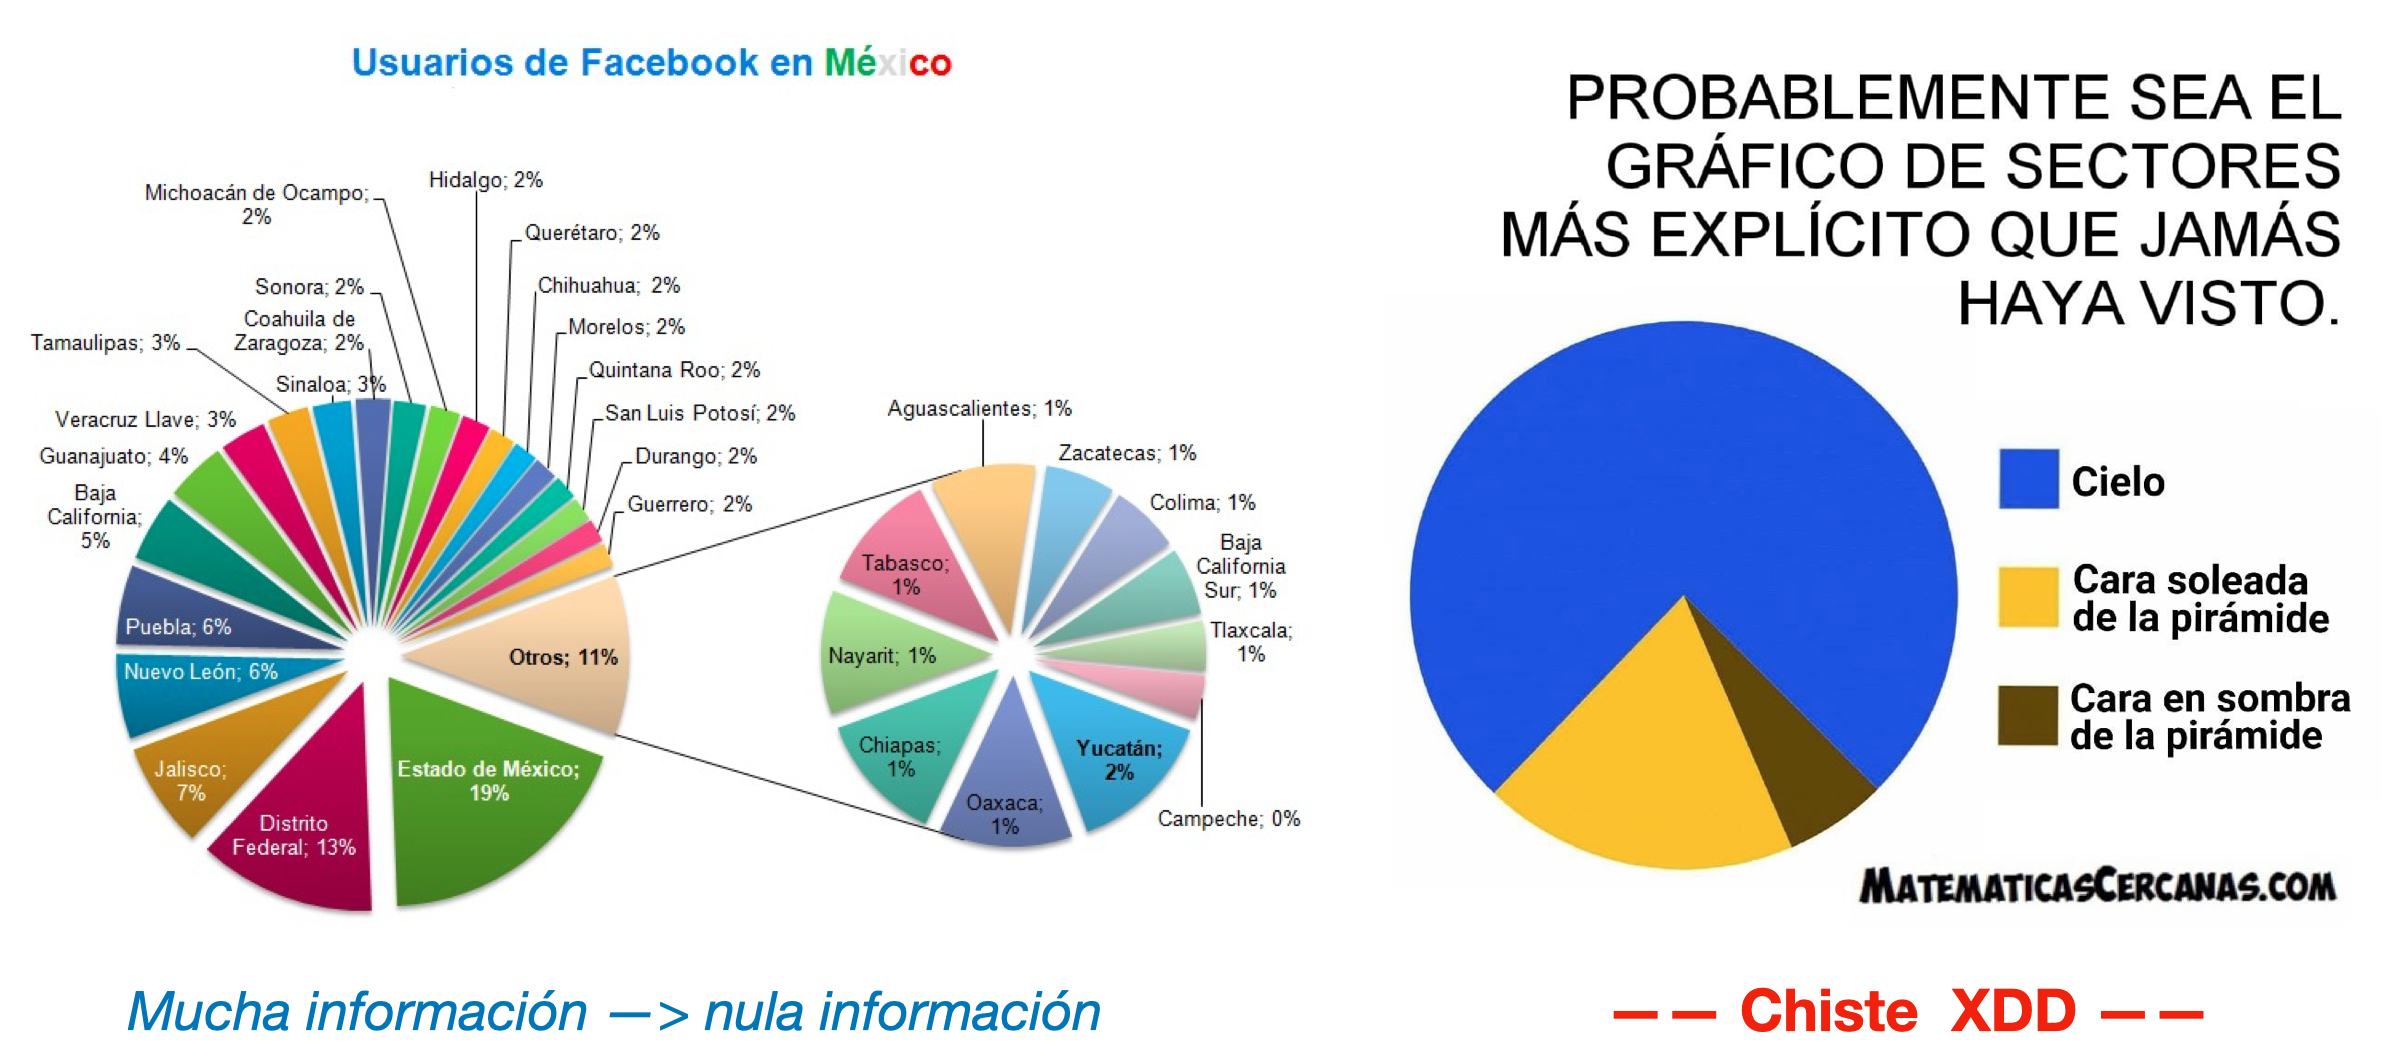
\includegraphics[width=1\textwidth]{imagenes/imagenes01/T01IM07.png}
		\end{figure}


\subsection{Otros tipos de representaciones gráficas en estadística}

	\begin{figure}[H]
			\centering
			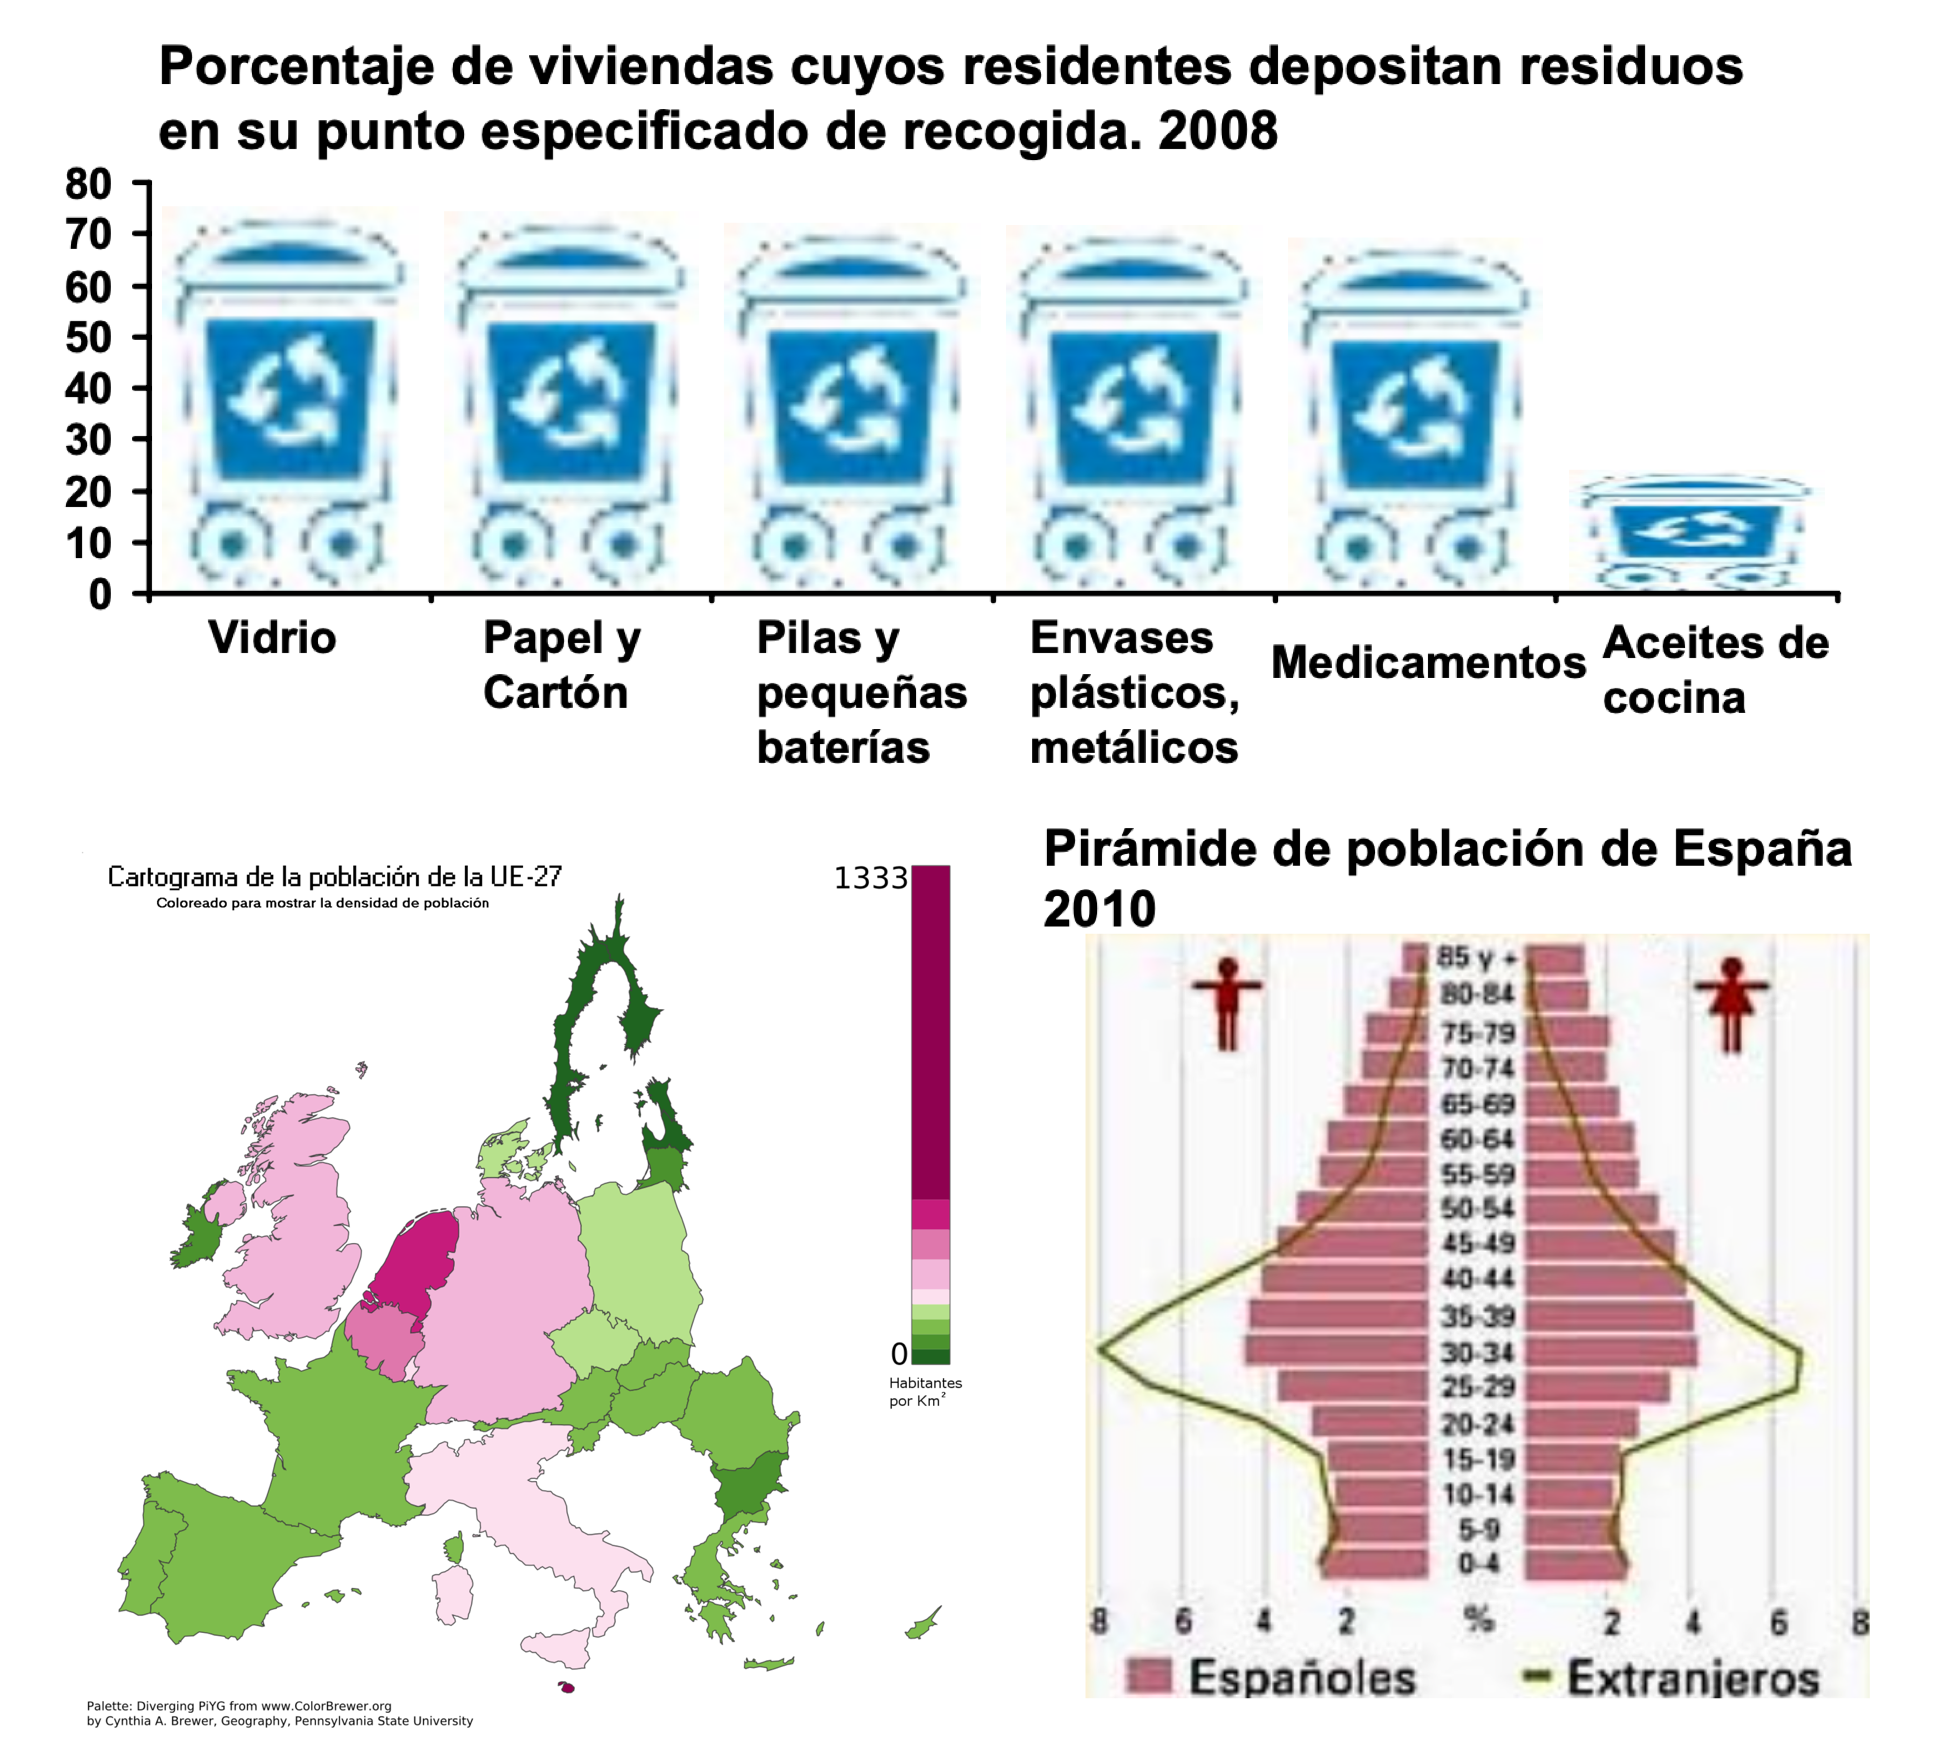
\includegraphics[width=.9\textwidth]{imagenes/imagenes01/T01IM08.png}
			\caption*{\footnotesize{Pictogramas, cartogramas y pirámides de población. (INE)}}
		\end{figure}

\begin{definition}
	. \textbf{Pictogramas}: se usan para datos no agrupados. Se representan con imágenes alusivas a la distribución y de tamaños proporcionales	(o repitiendo éstas un determinado número de veces) proporcional a la frecuencia. Tiene escasa precisión.
	
	\vspace{4mm} \textbf{Cartogramas}: se usan para representar sobre un mapa datos relacionados con un área geográfica.
	
	\vspace{4mm} \textbf{Pirámides de población}: son un par de histogramas verticales con un eje común, normalmente la edad y separando a izquierda y derecha por sexos.
	
\end{definition}



\subsection{Diagramas de tallos y hojas}

\begin{definition}
	. Un tipo de representación estadística que además es útil para el recuento de datos es el \textbf{diagrama de tallos y hojas} (Stem-and-Leaf Diagram) es un semigráfico que permite presentar la distribución de una variable cuantitativa. Consiste en separar cada dato en el último dígito (que se denomina hoja) y las cifras delanteras restantes (que forman el tallo).
\end{definition}


\vspace{5mm}%**********************

\begin{example}
	. Los datos siguientes corresponden a los tiempos de reacción de una muestra de $33$ sujetos, medidos en centésimas de segundo, son:
55, 51, 60, 56, 64, 56, 63, 63, 61, 57, 62, 50, 49, 70, 72, 54, 48, 53, 58, 66, 68, 45, 74, 65, 58, 61, 62, 59, 64, 57, 63, 52, 67.

\vspace{2mm} Construir el diagrama de tallos y hojas.

\begin{table}[H]
\centering
\begin{tabular}{c|ccccccccccccccc}
Tallos & \multicolumn{15}{l}{Hojas} \\ \hline
4 & 5 & 8 & 9 &  &  &  &  &  &  &  &  &  &  &  &  \\
5 & 0 & 1 & 2 & 3 & 4 & 5 & 6 & 6 & 7 & 7 & 8 & 8 & 9 &  &  \\
6 & 0 & 1 & 1 & 2 & 2 & 2 & 3 & 3 & 3 & 4 & 4 & 5 & 6 & 7 & 8 \\
7 & 0 & 2 & 4 &  &  &  &  &  &  &  &  &  &  &  & 
\end{tabular}
\end{table}
\end{example}


\subsection{Diagrama de cajas y bigotes}
Veremos este tipo de diagramas al final de la sección parámetros de posición.




\section{Parámetros estadísticos}

En los datos recogidos en tablas se pierde información si se agrupan en intervalos, aunque ello resulte necesario; aún se pierde más información al presentarlos en forma de gráficos pero se gana rapidez en la transmisión visual de la información. Pues, si lo que hacemos es asignar a toda la distribución estadística un limitado número de parámetros que la represente, la pérdida de la información es aún más grande pero inevitable para poder comparar rápidamente distintas distribuciones de datos, es lo que ocurre con los parámetros estadísticos.

Los parámetros estadísticos se dividen en:

\begin{adjustwidth}{20pt}{0pt}
\begin{itemize}
	\vspace{-2mm} \item Parámetros de centralización.
		\vspace{-2mm} \begin{itemize}
			\vspace{-1mm} \item Media aritmética (ponderada, geométrica, armónica).
			\vspace{-1mm} \item Moda.
			\vspace{-1mm} \item Mediana.
		\end{itemize}
	\vspace{-2mm} \item Parámetros de Posición.
		\begin{itemize}
			\vspace{-2mm} \item Cuartiles, Deciles, Percentiles.
		\end{itemize}
	\vspace{-2mm} \item Parámetros de dispersión.	
		\begin{itemize}
			\vspace{-1mm} \item Recorrido.
			\vspace{-1mm} \item Desviación media.
			\vspace{-1mm} \item Varianza. Desviación típica.
			\vspace{-1mm} \item Coeficiente de variación de Pearson.
		\end{itemize}
\end{itemize}
\end{adjustwidth}




\subsection{Parámetros de centralización}

\small{En matemáticas y estadística, una media o promedio es una medida de tendencia central. Resulta al efectuar una serie determinada de operaciones con un conjunto de números y que, en determinadas condiciones, puede representar por sí solo a todo el conjunto. Existen distintos tipos de medias, tales como la media geométrica, la media ponderada y la media armónica aunque en el lenguaje común, tanto en estadística como en matemáticas la elemental de todas ellas es el término que se refiere a la media aritmética.}

\vspace{5mm}%**********************
\begin{definition}
	. La \textbf{media aritmética} o simplemente media de una serie de valores aislados $\{x_1,x_2,\cdots , x_n\}$,  agrupados con sus frecuencias absolutas $\{n_1, n_2,\cdots n_n\}$, que se designa por $\boldsymbol{\bar{x}}$, se define como:

	
	$$\boxed{ \ \bold{ \bar{x}\ =\ \dfrac{x_1\cdot n_1+x_2\cdot n_2+\cdots +x_n \cdot n_n}{N}\ =\ \dfrac { \displaystyle \sum_{i=1}^n x_i\cdot n_i}{N} } \ }$$
donde $\ n_1+n_2+\cdots + n_n=\displaystyle \sum_{i=1}^n n_i=N \ $	 es el número total de datos.

\vspace{2mm} Si la distribución está agrupada en clases, $x_i$ representa a la \emph{`marca de clase'} o punto medio del intervalo.
\end{definition}

\vspace{5mm}%**********************
\begin{theorem}
	
	  \begin{enumerate}
 		\item La suma de las desviaciones respecto de la media es cero.
 		
 		$(x_1-\bar{x})\cdot n_1+ (x_2-\bar{x})\cdot n_2+\cdots +(x_n-\bar{x})\cdot n_n=0$
 		\item Si a cada valor de los datos $x_i$ se le añade una cantidad constante $b$, la media aumenta en $b$.
 		
 		$ \overline{ \{x_1+b, n_1;\ x_2+b,n_2; \ \cdots ; x_n+b, n_n \} } =\bar{x}+b$
 		\item Si a cada valor de los datos $x_i$ se le multiplica por una cantidad constante $a$, la media queda multiplicada por  $a$.
 		
 		$ \overline{ \{ax_1, n_1;\ ax_2,n_2; \ \cdots ; ax_n, n_n \} } =a\bar{x}$
 		
 		\item 	La media es \emph{`invariante'} frente a transformaciones lineales, cambio de origen y escala, de las variables; es decir si $X$ es una variable aleatoria e $Y$ es otra variable aleatoria que depende linealmente de $X$,  $\  Y = a\cdot X + b \ $ (donde $a$ representa la magnitud del cambio de escala y $b$ la del cambio de origen). De otro modo $\{x_i\}\to \{y_i=a\cdot x_i+b\}$ se tiene que:
 		
 		$\overline Y = a \cdot \overline X + b \qquad \text{ ó } \qquad \overline {\{y_i\}} = a \cdot \overline {\{x_i\}} + b$
 		
 		\end{enumerate}	
\end{theorem}

\begin{destacado}
Observaciones sobre la media aritmética:

\begin{adjustwidth}{20pt}{0pt}
\begin{itemize}
	
\item La media se puede hallar sólo para variables cuantitativas.
 
\item La media es independiente de las amplitudes de los intervalos.
 
\item La media es muy sensible a las puntuaciones extremas, también conocidos como valores atípicos.  

\item La media no se puede calcular si hay un intervalo con una amplitud indeterminada (clases abiertas, p.e. $[10,20[; \ [20,50[; \ \text{más de } 50$) ,  en este caso no es posible hallar la media porque no podemos calcular la marca de clase de último intervalo.	
\end{itemize}
\end{adjustwidth}
\end{destacado}


\begin{definition}
	. Otras medias:
	
	\textbf{Media ponderada}: $\ \bar{x_p}= \dfrac{\displaystyle \sum_{i_1}^N x_i\cdot p_i}{\displaystyle \sum_{i=1}^N p_i}; \qquad p_i \to \text{ pesos}$
	
	\vspace {3mm}  \small{A veces puede ser útil otorgar pesos o valores a los datos dependiendo de su relevancia para determinado estudio. Si a los valores $\{x_1,x_2,\cdots ,x_n\}$ se le conceden los pesos  $\{p_1,p_2,\cdots ,p_n\}$, la expresión anterior representa su `media ponderada'. Sirve para dar más peso a determinados valores.}
	
	\vspace{4mm} \textbf{Media Geométrica}: $\ \bar{x}_g=G= \displaystyle \sqrt[N]{x_1^{n_1} \cdot x_2^{n_2} \cdots x_n^{n_n}}$
	
	\vspace {3mm} \small{La media geométrica es un promedio muy útil en conjuntos de números que son interpretados en orden de su producto, no de su suma (tal y como ocurre con la media aritmética). Por ejemplo, las velocidades de crecimiento.}
	
	\vspace{4mm} \textbf{Media Armónica}: $\bar{x}_a=H=\dfrac{N} { \displaystyle \sum_{i=1}^n { \dfrac {n_i}{x_i} } } $
	
	\vspace {3mm} \small{La media armónica es un promedio muy útil en conjuntos de números que se definen en relación con alguna unidad, por ejemplo la velocidad (distancia por unidad de tiempo)}.
\end{definition}


\vspace{5mm}%**********************
\begin{example}
	. Cálculo de la media del ejemplo \ref{ejparamedia}:	
	
\begin{multicols}{2}
% Please add the following required packages to your document preamble:
% \usepackage{multirow}
\begin{table}[H]
\small
\centering
\begin{tabular}{cc|c|clc}
\cline{1-4}
\multicolumn{1}{|c|}{\textbf{edades}} & \textbf{$x_i$} & \textbf{$n_i$} & \multicolumn{1}{c|}{\textbf{$x_i\cdot n_i$}} & $\quad$ & \multirow{6}{*}{} \\ \cline{1-4}
\multicolumn{1}{c|}{[2,6[}            & 4              & 5              & 20                                           &         &                   \\
\multicolumn{1}{c|}{[6,10[}           & 8              & 7              & 56                                           &         &                   \\
\multicolumn{1}{c|}{[10,14[}          & 12             & 11             & 132                                          &         &                   \\
\multicolumn{1}{c|}{[14,18[}          & 16             & 3             & 48                                          &         &                   \\ \cline{3-4}
                                      &                & 26             & \multicolumn{1}{c|}{256}                     &         &                   \\ \cline{3-4}
\end{tabular}
\end{table}

\begin{center}
$\quad$

$\boldsymbol{\bar{x}=} \dfrac{\sum x_i\cdot n_i}{\sum n_i}=$

$=\dfrac{256}{26}=\boldsymbol{9.85}$
\end{center}

\end{multicols}
\end{example}

\vspace{5mm}%**********************
\begin{example}
	. Una empresa ha generado un 20 \% de rentabilidad el primer año, un 15 \% el segundo año, un 33 \% el tercer año y un 25 \% el cuarto año. Si  sumamos las cantidades y dividir entre cuatro, este valor no representa nada en correcto. Para calcular la media de varios porcentajes debemos hacer uso de la media geométrica. Aplicado al caso anterior, tendríamos lo siguiente:

\vspace{2mm}$\bar{x}_g=\sqrt[4]{1.20 \cdot 1.15 \cdot 1.33 \cdot 1.25}=1.23 \ \to \ 23 \%$ de beneficio medio en los cuatro años, es decir, si cada año hubiese ganado un 23 \%, hubiera ganado lo mismo que ganando un 20 \% el primer año, un 15 \% el segundo, un 33 \% el tercero y un 25 \% el último año.
\end{example}

\vspace{5mm}%**********************
\begin{example}
	. Un coche recorre $100 \ \mathrm{km}$ a una velocidad de $60 \ \mathrm{Km/h}$, otros $100 \ \mathrm{km}$ a 	$70 \ \mathrm{Km/h}$ y otros $100 \ \mathrm{km}$ a $80 \ \mathrm{Km/h}$. La velocidad media viene determinada por la \emph{media armónica}:
	
	\vspace{4mm} $\bar{x}_h=\dfrac{3}{\dfrac 1{60}+\dfrac 1{70} + \dfrac 1{80}}=69.04\ \mathrm{km/h} \quad $
	\begin{tiny}\textcolor{gris}{$\left( \text{velocidad media}=\dfrac{\text{espacio total}}{\text{tiempo empleado}} \right)$}\end{tiny}
\end{example}

\vspace{5mm}%**********************
\begin{definition}
	. Dada una serie estadística, se llama \textbf{moda}, \textbf{mo}, al valor de la serie que tiene mayor frecuencia absoluta.
	
	\vspace{2mm} Una serie estadística puede ser \emph{plurimodal} (tener más de una moda) y \emph{amodal}, sin moda (si todas las frecuencias son iguales).
\end{definition}

\vspace{5mm}%**********************
\begin{theorem}
	. La \textbf{moda para datos agrupados} se obtiene aplicando la fórmula:
	
	$$\boldsymbol{ mo=L_k+\dfrac{n_k-n_{k-1}}{(n_k-n_{k-1})+(n_k-n_{k+1})}\cdot c_k }\ ,\quad \text{ donde:}	$$
	
	\vspace{2mm} \begin{itemize}
	\vspace{-2mm} \item $L_k:\ $ extremo inferior de la \textbf{clase modal} (\emph{clase con mayor frecuencia absoluta})	.
	\vspace{-2mm} \item $n_k:\ $ frecuencia absoluta de la clase modal.
	\vspace{-2mm} \item $n_{k-1} \text{ y } n_{k+1}:\ $ frecuencias absolutas de las clases anterior y posterior a la clase modal.
	\vspace{-2mm} \item $c_k:\ $ amplitud de las clase modal.
	\end{itemize}

\end{theorem}

\vspace{5mm}%**********************
\begin{example}
	. Cálculo de la moda del ejemplo \ref{ejparamedia}:	
	
\begin{multicols}{2}
\small
\begin{table}[H]
\centering
\begin{tabular}{cc|c|}
\hline
\multicolumn{1}{|c|}{\textbf{edades}} & \textbf{$x_i$} & \textbf{$n_i$} \\ \hline
\multicolumn{1}{c|}{[2,6[}            & 4              & 5              \\
\multicolumn{1}{c|}{[6,10[}           & 8              & 7              \\
\multicolumn{1}{c|}{[10,14[}          & 12             & 11             \\
\multicolumn{1}{c|}{[14,18[}          & 16             & 3             \\ \cline{3-3} 
                                      &                & 26             \\ \cline{3-3} 
\end{tabular}
\end{table}
\textbf{Intervalo modal:} $\boldsymbol{ [10,14[ }$

$n_i=n_3=11;\ n_{i-1}=n_2=7;\ n_{i+1}=n_4=3$

$L_i=L_3=10;\ c_i=4$

$mo=10+\dfrac{(11-7)}{(11-7)+(11-3)}\cdot 4$

$mo=11.33$

\end{multicols}
	
En muchas ocasiones es suficiente con determinar el intervalo modal (el de mayor frecuencia absoluta).
\end{example}

\vspace{5mm}%**********************
\begin{definition}
	. Dada una serie estadística de un \emph{número impar de valores}, se llama \textbf{mediana} , \textbf{me}, al valor central de la serie, es decir, aquel valor tal que	 la mitad de los valores son mayores o iguales a él y la otra mitad, menores o iguales a él. Suponiendo la serie estadística \emph{ordenada en sentido creciente}.
	
	\vspace{2mm} Si la serie tiene un \emph{número par de valores}, se define la media como la \emph{semisuma de los dos valores centrales}.
\end{definition}

Para un determinado número de individuos $N$, el valor central viene determinado por $ \frac{N+1}{2}$. Si el resultado es decimal, hay dos individuos centrales, el  $\frac{N}{2}$ y el $\frac N 2 + 1$.

\vspace{5mm}%**********************
\begin{theorem}
	. Para datos agrupados, si la media está en la clase $[L_k,L_{k+1}[$, de frecuencia absoluta $n_k$, frecuencia absoluta acumulada de la clase anterior a la mediana $N_{k-1}$ y de  $c_i$  amplitud de la clase mediana, la \textbf{mediana} la determina la fórmula:	
	
	$$\boldsymbol{ me=L_k+\dfrac{\dfrac N 2 - N_{k-1}}{n_{k}}\cdot c_k }$$
\end{theorem}


\vspace{5mm}%**********************
\begin{example}
. --- En la serie: $2,4,6,\boldsymbol{8},9,10,12$, la mediana es $\ me=8$

\vspace{2mm} --- En la serie: $2,2,3,\boldsymbol{5}, \boldsymbol{8}, 10, 10, 12$, la mediana es $\ me=\dfrac{5+8}{2}=6.5$

\vspace{2mm} --- En la serie del ejemplo \ref{ejparamedia}, la mediana será:

\begin{multicols}{2}
\begin{table}[H]
\small
\centering
\begin{tabular}{cc|c|cc}
\cline{1-4}
\multicolumn{1}{|c|}{\textbf{edades}} & \textbf{$x_i$} & \textbf{$n_i$} & \multicolumn{1}{c|}{\textbf{$N_i$}} & \textcolor{gris}{$H_i$} \\ \cline{1-4}
\multicolumn{1}{c|}{[2,6[}            & 4              & 5              & 5                                   & \textcolor{gris}{0.19}  \\
\multicolumn{1}{c|}{[6,10[}           & 8              & 7              & 12                                  & \textcolor{gris}{0.46}  \\
\multicolumn{1}{c|}{[10,14[}          & 12             & 11             & 23                                  & \textcolor{gris}{0.88}  \\
\multicolumn{1}{c|}{[14,18[}          & 12             & 3              & 26                                  & \textcolor{gris}{1.00}  \\ \cline{3-3}
                                      &                & 26             &                                     &       \\ \cline{3-3}
\end{tabular}
\end{table}
$\dfrac N 2=13; \ L_k=10,$

$n_k=11; \ N_{k-1}=12$

$k=3$,  clase mediana $[10,14[$

$\quad$

$me=10+\dfrac{13-12}{10}\cdot 4=10.36$

\end{multicols}
En ocasiones es suficiente con determinar la clase mediana.
\end{example}

Se puede obtener un valor aproximado de la mediana a través del histograma de frecuencias relativas acumuladas \textcolor{gris}{(ahora, la línea poligonal no une los puntos medios de cada clase sino los extremos superiores de cada clase)}.

	\begin{figure}[H]
			\centering
			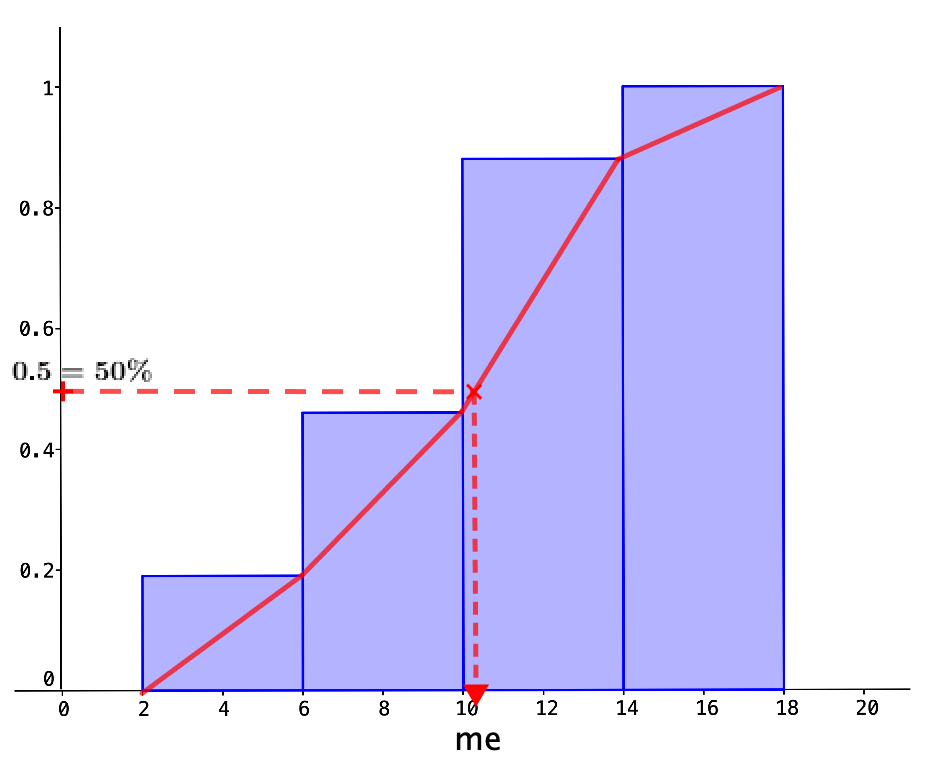
\includegraphics[width=.75\textwidth]{imagenes/imagenes01/T01IM09.png}
		\end{figure}

Tanto en el caso de la mediana como en el de la moda para datos agrupados, las fórmulas se deducen la una \emph{simple interpolación lineal}.


\begin{figure}[H]
			\centering
			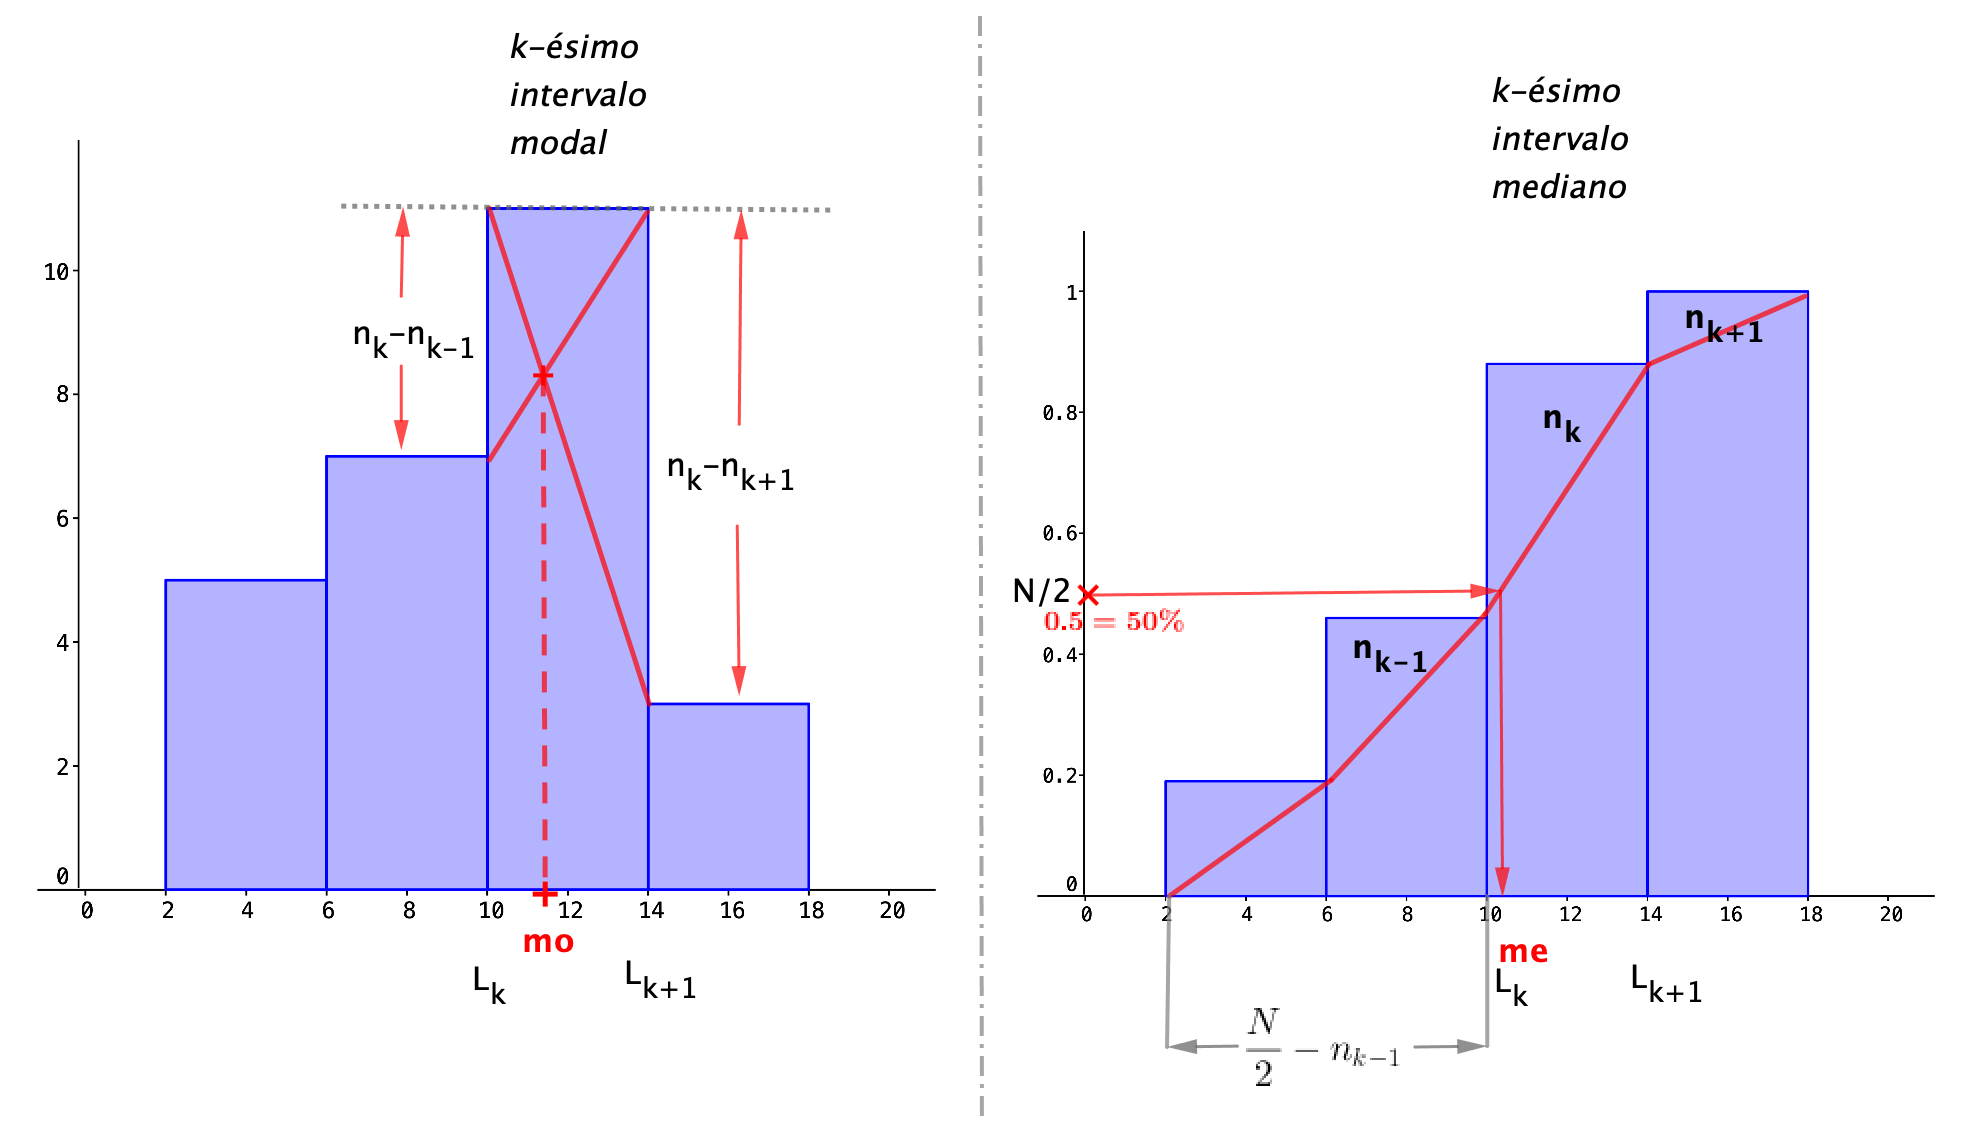
\includegraphics[width=1.05\textwidth]{imagenes/imagenes01/T01IM10.png}
		\end{figure}


\vspace{5mm}%**********************		
\begin{ejemplo}
	
\begin{ejre}

Calcular Media, moda y mediana para la siguiente serie estadística.

\begin{multicols}{2}
\begin{footnotesize}
\begin{table}[H]
\small
\centering
\begin{tabular}{rr|r|r|r}
\hline
\multicolumn{1}{|c|}{\textbf{Clases}} & \multicolumn{1}{c|}{\textbf{$x_i$}} & \multicolumn{1}{c|}{\textbf{$n_i$}} & \multicolumn{1}{c|}{\textbf{$N_i$}} & \multicolumn{1}{c|}{\textbf{$x_i\cdot n_i$}} \\ \hline
\multicolumn{1}{r|}{[20,30[}          & 25                                  & 20                                  & 20                                  & 500                                          \\
\multicolumn{1}{r|}{[30,40[}          & 35                                  & 35                                  & 25                                  & 1225                                         \\
\multicolumn{1}{r|}{[40,50[}          & 45                                  & 50                                  & 105                                 & 2250                                         \\
\multicolumn{1}{r|}{[50,60[}          & 55                                  & 49                                  & 154                                 & 2695                                         \\
\multicolumn{1}{r|}{[60,70[}          & 65                                  & 25                                  & 179                                 & 1625                                         \\
\multicolumn{1}{r|}{[70,80[}          & 75                                  & 15                                  & 194                                 & 1125                                         \\
\multicolumn{1}{r|}{[80,90[}          & 85                                  & 6                                   & 200                                 & 510                                          \\ \cline{3-3} \cline{5-5} 
                                      &                                     & 200                                 &                                     & \multicolumn{1}{r|}{9930}                    \\ \cline{3-3} \cline{5-5} 
\end{tabular}
\end{table}
\end{footnotesize}
\hspace{1cm} \begin{footnotesize}$\bar{x}=\dfrac{9930}{200}$\end{footnotesize}

\hspace{1cm} $\boldsymbol{ \bar{x}=49.65 }$

\hspace{1cm} \begin{scriptsize}$mo=40+\dfrac{50-35}{(50-35)+(50-49)} 10$\end{scriptsize}

\hspace{1cm} $\boldsymbol{ mo=49.38 }$

\hspace{1cm} \begin{footnotesize}$me=40+\dfrac{\dfrac{200}{2}-55}{50}\cdot 10$\end{footnotesize}

\hspace{1cm} $\boldsymbol{ me=49.00 }$

\end{multicols}

\end{ejre}
\end{ejemplo}


\vspace{10mm}%**********************
\begin{myalertblock}{Ventajas y desventajas de la medidas de tendencia central.}

%\begin{footnotesize}
\begin{itemize}

\item MEDIA

	\begin{itemize}
	\item Ventajas 
		\begin{itemize}
		\item Es la medida de tendencia central más usada.
		\item Emplea en su cálculo toda la información disponible.
		\item Es un valor único.
		\item Se emplea a menudo en cálculos estadísticos posteriores.
		\item Tiene un sentido claro como valor de tendencia del agrupamiento de los datos.
		\item Es sensible a cualquier cambio en los datos (puede ser usado como un detector de variaciones en los datos).
		\item Es útil para llevar a cabo procedimientos estadísticos como la comparación de medias de varios conjuntos de datos.
		\item Presenta rigor matemático.
		\item En la gráfica de frecuencia representa el centro de gravedad.
		\end{itemize}
	\item Desventajas
		\begin{itemize}
		\item Es sensible a los valores extremos.
		\item No es recomendable emplearla en distribuciones muy asimétricas.
		\item Si se emplean variables discretas, la media aritmética puede no pertenecer al conjunto de valores de la variable.
		\item No se puede calcular para datos cualitativos.
		\item No se puede calcular para datos que tengan clases de extremo abierto, tanto superior como inferior.
		\end{itemize}
	\end{itemize}

\item MEDIANA
	\begin{itemize}
	\item Ventajas:
		\begin{itemize}
		\item No se ve influenciada por valores extremos, ya que solo influyen los valores centrales.
		\item Fácil de entender.
		\item Se puede calcular para cualquier tipo de datos cuantitativos, incluso los datos con clase de extremo abierto.
		\item Es la medida de tendencia central más representativa en el caso de variables que solo admiten la escala ordinal.
		\end{itemize}
	\item Desventajas
		\begin{itemize}
		\item No utiliza en su cálculo toda la información disponible.
		\item No pondera cada valor por el número de veces que se ha repetido.
		\item Hay que ordenar los datos antes de determinarla.
		\end{itemize}
	\end{itemize}

\item MODA
	\begin{itemize}
		\item Ventajas
		\begin{itemize}
		\item No requiere cálculos.
		\item Puede usarse para datos tanto cuantitativos como cualitativos.
		\item Fácil de interpretar.
		\item No se ve influenciada por valores extremos.
		\item Se puede calcular en clases de extremos abiertos.
		\end{itemize}
	\item Desventajas
		\begin{itemize}
		\item Solo tiene significado en el caso de una gran cantidad de datos.
		\item No utiliza toda la información disponible.
		\item Difícil de interpretar si los datos tiene 3 o más modas.
		\end{itemize}
	\end{itemize}

\end{itemize}
%\end{footnotesize}
	
\end{myalertblock}


\vspace{5mm}%**********************
\begin{myexampleblock}{?`Cuál de los parámetros de posición es más representativo?}
\begin{small}

Cuando estudiamos las medidas de tendencia central, como la media, la moda y la mediana, nos preguntamos, tantas medidas y al final,  ?`cuál es la mas representativa?, ?`es suficiente con las medidas de tendencia central para caracterizar a un conjunto de datos?\footnote{Del blog  ``https://estadisticaestasahi.blogspot.com’’}


\vspace{2mm} Aclaremos esto con un ejemplo (tomado de ``Probabilidades y Estadística. Su Enseñanza’’ de J. Foncuberta, Red Federal de Formación Docente Continua, MECyT, 1996).


\vspace{2mm} El Sr J., gobernante de un remoto país, se jactaba de que el salario medio en su país era de 3000 \euro. El señor Modulador, de visita por esos lugares observó las extrañas costumbres de sus habitantes: vestían muy mal, comían peor, se guarecían donde podían y padecían graves enfermedades. Como el señor Modulador es sumamente ingenuo creyó que en ese país el ahorro más que una virtud era una obsesión pero por más que preguntó nadie supo sacarlo de su perplejidad. Hasta que cierto día encontró a un colega Modulador de aquellas regiones que le aclaró el misterio: sucedía que entre 1 millón de habitantes, la renta se distribuía así:



\begin{table}[H]
\footnotesize
\centering
\begin{tabular}{cr|r|r}
 & \multicolumn{1}{c|}{\textbf{Renta}} & \multicolumn{1}{c|}{\textbf{perceptores}} & \multicolumn{1}{c}{\textbf{\begin{tabular}[c]{@{}c@{}}promedio\\ per cápita\end{tabular}}} \\ \cline{2-4} 
\multicolumn{1}{c|}{\textbf{\begin{tabular}[c]{@{}c@{}}Sr. \\ J\end{tabular}}} & 1.800.000.000 & 1 & 1.800.000.000 \\ \cline{1-1}
\multicolumn{1}{c|}{\textbf{\begin{tabular}[c]{@{}c@{}}Allegados\\ Sr. J\end{tabular}}} & 1.000.120.000 & 999 & 1.0001.121 \\ \cline{1-1}
\multicolumn{1}{c|}{\textbf{\begin{tabular}[c]{@{}c@{}}Resto de \\ habitantes\end{tabular}}} & 199.880.000 & 999.000 & 200 \\ \cline{2-4} 
\multicolumn{1}{c|}{} & \multicolumn{1}{c|}{\textbf{3.000.000.000}} & \multicolumn{1}{c|}{\textbf{1.000.000}} & \multicolumn{1}{c|}{\textbf{3.000}} \\ \cline{2-4} 
\end{tabular}
\caption*{\small{(cualquier parecido con la realidad es mera coincidencia)}}
\end{table}


\begin{multicols}{2}
\vspace{2mm} Efectivamente el salario promedio era de  3.000 \euro! , ahora bien esto no es para nada representativo de la realidad del salario en dicho país!!! o si?

\vspace{2mm} Desde entonces el Sr. Modulador desconfía mucho del valor medio. 

	\begin{figure}[H]
			\centering
			
\includegraphics[width=.2\textwidth]{imagenes/imagenes01/T01IM11.png}
		\end{figure}
\end{multicols}	

\vspace{2mm} No es lo mismo un país donde el salario medio es de 3.000 \euro con valores máximo y mínimo 3.500 y 2.000 que otro como el del ejemplo con igual valor medio pero con valores extremos 1.800.000.000 \euro y 200 \euro.

\vspace{2mm} Sin duda en el primer caso los datos están menos dispersos que en el segundo, de hecho en el ejemplo podemos hablar de valores extremos (lo que gana Don J!). Una de las desventajas del valor medio es justamente la sensibilidad a valores extremos y en este ejemplo vemos claramente como la media es `tironeada' hacia arriba por estos valores extremos.

\vspace{2mm} Y que pasaría si para el mismo ejemplo, simplificando la situación y pensando que los salarios son exactamente los que figuran en la columna promedio per cápita, calculáramos la Mediana? Como la hallamos? ordenando todos los datos de menor a mayor y encontrando el valor central. Tenemos un millón de datos, donde una vez ordenados el valor central sería el promedio del dato en la posición 500.000 y la 500.001. Si ordenamos y los primeros 999.000 ganan 200 \euro, entonces 
Mediana=(200+200)/2=200 \euro.

\vspace{2mm} En este caso y en este ejemplo cuál de las dos medidas es más representativa? la media o la mediana? sin duda que la MEDIANA! Lo mismo podríamos decir de la MODA (también 200 \euro).

\vspace{2mm} ?`Cómo podemos cuantificar esta variabilidad del conjunto de datos? Necesitamos una medida para la desviación o dispersión de los datos, y es allí donde aparecen las medidas de variabilidad. Las vemos en el siguiente apartado.  
\end{small}

\end{myexampleblock}

Media, mediana y moda coinciden en las distribuciones ``normales'', aprenderemos que son estas distribuciones en el tema \ref{distprob} de `distribuciones de probabilidad'.

\subsection{Parámetros de posición}
	
	Aunque hemos definido a la \textbf{mediana} como un \textbf{parámetro de centralización}, en realidad es un \textbf{parámetro de posición}, aunque representa la \emph{posición central} de la distribución (o serie estadística) y por eso se puede considerar en los dos tipos de parámetros.
	
	

	Los \textbf{cuantiles} son medidas de posición y proporcionan los valores en que se encuentra la distribución.	 Reciben distintos nombres según el número de partes en que si divida la distribución o serie estadística, así, se habla de \textbf{Cuartiles, Deciles y Percentiles}.


\vspace{5mm}%**********************
\begin{definition}
	. \textbf{Cuarliles: $\boldsymbol{ Q_1,\ Q_2=me,\ Q_3 }$}, dividen a la población $(N)$ en cuatro partes iguales $(N/4,\  N/2,\  3N/4)$. Entre dos cuartiles sucesivos se encuentra el $25\%$ de la población.
	
	\begin{figure}[H]
			\centering
			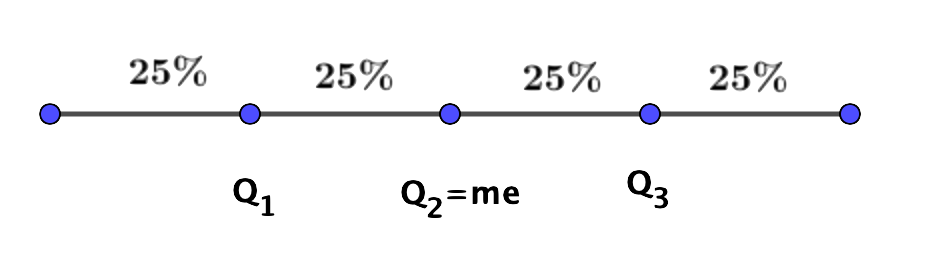
\includegraphics[width=.7\textwidth]{imagenes/imagenes01/T01IM12.png}
	\end{figure}
\end{definition}

Evidentemente, $\ Q_2=me$.

\vspace{5mm}%**********************	
\begin{theorem}
	. Para datos agrupados, como en la mediana, 
	
	$$\boxed{\ \boldsymbol{Q_1=L_k+\dfrac{\dfrac{N}{4}-N_{k-1}}{n_k}\cdot c_k} \ }$$
	
	$$\boxed{\ \boldsymbol{Q_2=L_k+\dfrac{\dfrac{N}{2}-N_{k-1}}{n_k}\cdot c_k \ = \ me}  \ } $$
	
	$$ \boxed{\ \boldsymbol{Q_3=L_k+\dfrac{\dfrac{3N}{4}-N_{k-1}}{n_k}\cdot c_k} \ }$$
\end{theorem}

\vspace{5mm}%**********************
\begin{definition}
	. Los \textbf{Deciles} son 9 valores, $D_1,\ D_2, \ D_3,  \cdots , D_9$, que dividen a la población en $10$ partes iguales. Entre dos deciles consecutivos se encuentra el $10\%$ de la población.	
	
	\begin{figure}[H]
			\centering
			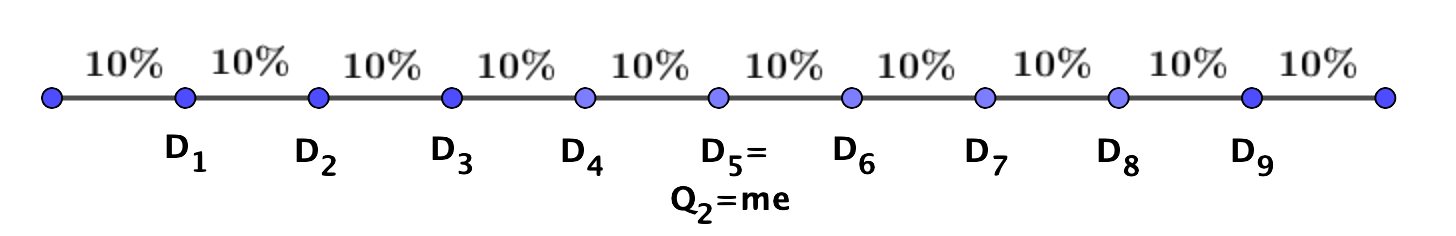
\includegraphics[width=.9\textwidth]{imagenes/imagenes01/T01IM13.png}
	\end{figure}
\end{definition}

Evidentemente, $\ D_5=Q_2=me$.

\vspace{5mm}%**********************
\begin{theorem}
	. Para datos agrupados, como en la mediana, 
	
	$$\boxed{\ \boldsymbol{D_m=L_k+\dfrac{\dfrac{mN}{10}-N_{k-1}}{n_k}\cdot c_k} \ }\; \qquad m=1,2,3,\cdots , 9$$
	
\end{theorem}
	
\vspace{5mm}%**********************
\begin{definition}
	. Los \textbf{Percentiles} son 99 valores, $P_1,\ P_2, \ P_3,  \cdots , P_{67}, \cdots, P_{99}$, que dividen a la población en $100$ partes iguales. Entre dos percentiles consecutivos se encuentra el $1\%$ de la población.	
\end{definition}

\vspace{5mm}%**********************
\begin{theorem}
	. Para datos agrupados, como en la mediana, 
	
	$$\boxed{\ \boldsymbol{P_m=L_k+\dfrac{\dfrac{mN}{100}-N_{k-1}}{n_k}\cdot c_k} \ }\; \qquad m=1,2,3,\cdots , 99$$
\end{theorem}

Evidentemente, $P_{50}=D_5=Q_2=me;\ P_{25}=Q_1;\ P_{75}=Q_3$

Como ocurría con la mediana, se puede obtener un \underline{valor aproximado de los cuartiles} a través del histograma de frecuencias relativas acumuladas \textcolor{gris}{(ahora, la línea poligonal no une los puntos medios de cada clase sino los extremos superiores de cada clase y el extremo inferior de la primera clase)}.

	\begin{figure}[H]
			\centering
			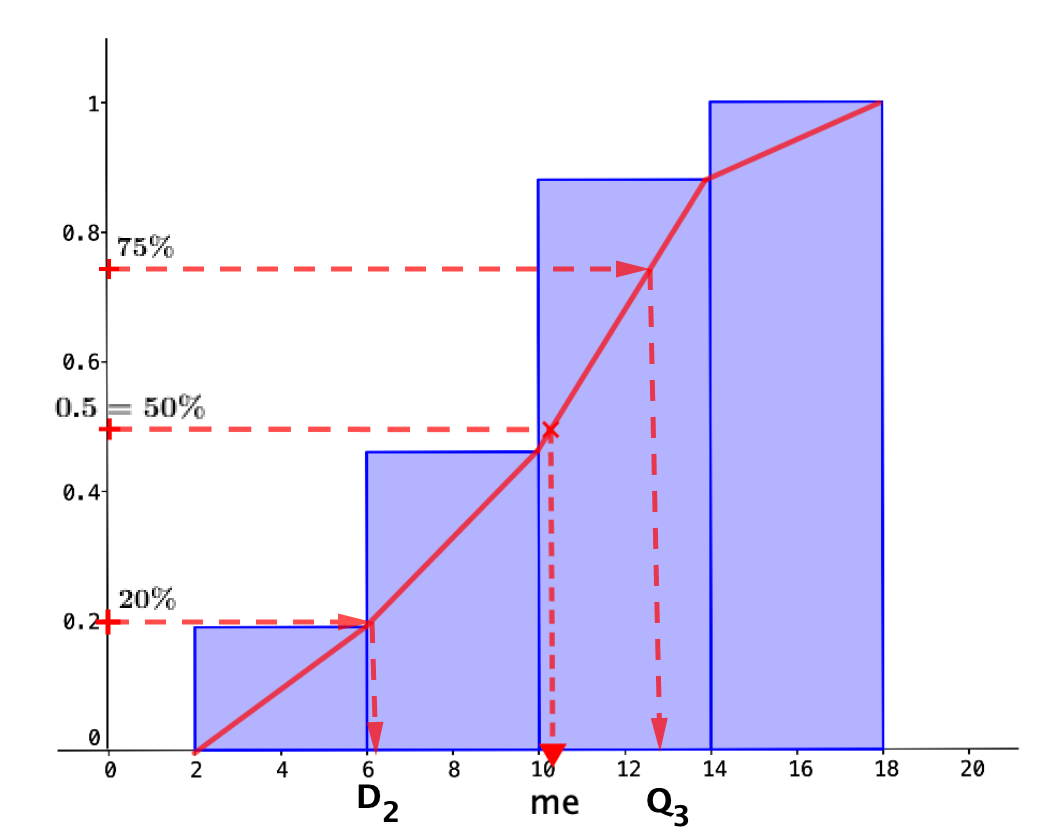
\includegraphics[width=.75\textwidth]{imagenes/imagenes01/T01IM09_copia.png}
	\end{figure}

\vspace{5mm}%**********************
\begin{example}
	. Los datos siguientes corresponden a los tiempos de reacción de una muestra de $33$ sujetos, medidos en centésimas de segundo, son:
55, 51, 60, 56, 64, 56, 63, 63, 61, 57, 62, 50, 49, 70, 72, 54, 48, 53, 58, 66, 68, 45, 74, 65, 58, 61, 62, 59, 64, 57, 63, 52, 67.

\vspace{2mm} Calcúlese  la moda, la mediana, el primer y el tercer cuartil, directamente a partir de los datos.	Calcúlese, así mismo, los deciles segundo y quito y los percentiles 33 y 58.

\vspace{4mm}  Construimos un diagrama de tallos y hojas, que nos permitirá contar los datos y tenerlos ordenados (una forma alternativa a las tablas de frecuencias absolutas).

\begin{table}[H]
\centering
\begin{tabular}{c|ccccccccccccccc}
Tallos & \multicolumn{15}{c|}{Hojas} \\ \hline
4 & 5 & 8 & 9 &  &  &  &  &  &  &  &  &  &  &  &  \\
5 & 0 & 1 & 2 & 3 & 4 & 5 & 6 & 6 & 7 & 7 & 8 & 8 & 9 &  &  \\
6 & 0 & 1 & 1 & 2 & 2 & 3 & 3 & 3 & 3 & 4 & 4 & 5 & 6 & 7 & 8 \\
7 & 0 & 2 & 4 &  &  &  &  &  &  &  &  &  &  &  & 
\end{tabular}
\end{table}

\begin{multicols}{2}
$mo=63$; 

$ (33+1)/2 = 17 \to me=x_{17}=60$

$\frac 1 4 33= 8.25 \to Q_1=x_9=55$

$\frac 3 4 33=24.75 \to Q_3=x_{25}=34$

$D_2=\frac 2 {10} 33 = 6.6 \to D_2=x_{7}=53$

$D_5=me=60$

$\frac {33}{100}33=10.89 \to  P_{33}=x_{11}=66$

$\frac {58}{100}33=19.14 \to  P_{58}=x_{20}=68$
\end{multicols}

\end{example}


\vspace{5mm}%**********************
\begin{example}

	 Con los datos del ejemplo anterior, construya una tabla estadística  agrupados los datos en 5 intervalos de igual amplitud, calcule la mediana, el primer y el tercer cuartil.	Calcúlese, así mismo, los deciles segundo y quito y los percentiles 33 y 58.

\vspace{4mm} \begin{small}Para llegar a la anterior tabla se ha calculado en primer lugar el rango de la distribución que es el mayor valor 74 menos el menor 45, lo que nos da 29. Como 29 no es divisible entre 5 redondeamos hasta el valor más próximo por exceso que es 30, dividiendo este rango entre el número de intervalos que deseamos, cinco, obtenemos la amplitud que deben tener los intervalos, seis. A partir del primer valor, 45 se han calculado los restantes extremos sumando 6, sucesivas veces. Posteriormente se ha contado el número de observaciones comprendidas dentro de cada intervalo, recuérdese que los intervalos se toman abiertos a la derecha, y de esta forma se han obtenido las frecuencias que aparecen en la tabla, en la que se han añadido las frecuencias acumuladas.\end{small}

\begin{multicols}{2}
\begin{table}[H]
\begin{tabular}{crr}
\textbf{Clases}                  & \multicolumn{1}{|c|}{\textbf{$n_i$}} & \multicolumn{1}{c}{\textbf{$N_i$}} \\ \hline
\multicolumn{1}{c|}{{[}45,51{[}} & \multicolumn{1}{r|}{4}             & 4                                  \\
\multicolumn{1}{c|}{{[}51,57{[}} & \multicolumn{1}{r|}{6}             & 10                                 \\
\multicolumn{1}{c|}{{[}57,63{[}} & \multicolumn{1}{r|}{11}            & 21                                 \\
\multicolumn{1}{c|}{{[}63,69{[}} & \multicolumn{1}{r|}{9}             & 30                                 \\
\multicolumn{1}{c|}{{[}69,75{[}} & \multicolumn{1}{r|}{3}             & 33                                
\end{tabular}
\end{table}
--- Intervalo modal: $\ [57,63[$

--- $mo=$ \begin{scriptsize}
 $57+\dfrac{11-6}{(11-6)+(11-9)}6$	
\end{scriptsize} $=61.3$

--- \begin{scriptsize}
$33/2=16.5 \to $ \end{scriptsize} Int. mediano: $\ [57,63[$


--- $me=$\begin{scriptsize}
 $57+\dfrac{16.5-10}{11}6$	
\end{scriptsize}$=60.5$
\end{multicols}
--- $25\% 33=8,25 \to [51,57 [ \to Q_1=57+\dfrac{8.25-4}{6}\ 6=55.3$

--- $75\% 33=24,75 \to [63,69 [ \to Q_3=63+\dfrac{24.75-21}{9}\ 6=65.5$

--- $20\% 33=6,6 \to [51,57 [ \to D_2=51+\dfrac{6.6-4}{6}\ 6=53.6$

--- $D_5=me=60.5$

--- $33\% 33=10.9 \to [57,63 [ \to P_{33}=57+\dfrac{10.9-10}{11}\ 6=57.1$

--- $58\% 33=19,1 \to [57,63 [ \to P_{58}=57+\dfrac{19.1-10}{11}\ 6=62.0$

\vspace{4mm} De manera aproximada, aparece en la figura siguiente.
\end{example}

\begin{figure}[]
			\centering
			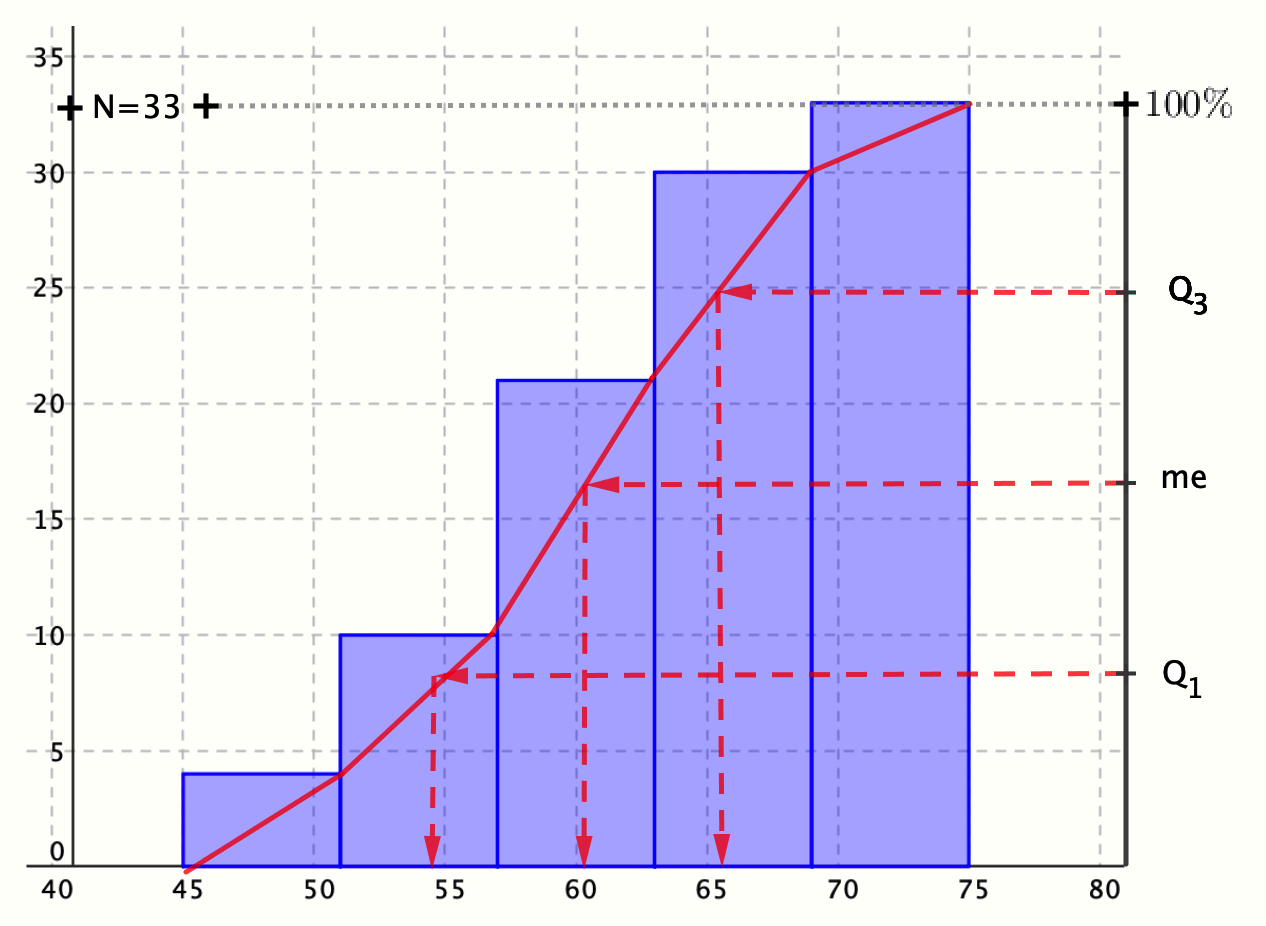
\includegraphics[width=.75\textwidth]{imagenes/imagenes01/T01IM14.png}
			\caption*{Histograma de frecuencias relativas acumuladas. del ejemplo 1.15}
	\end{figure}

\vspace{15mm}%**********************
\begin{ejemplo}
\begin{ejre}
Para la siguiente distribución estadística, responder a las  preguntas que se formulan.

\vspace{5mm}%*********************
\begin{multicols}{2}
\begin{table}[H]
\begin{tabular}{c|r|r}
\textbf{$x_i$} & \multicolumn{1}{c|}{\textbf{$n_i$}} & \multicolumn{1}{c}{\textbf{$N_i$}} \\ \hline
{[}0,10{[}     & 8                                   & 8                                  \\
{[}10,20{[}    & 22                                  & 30                                 \\
{[}20,30{[}    & 32                                  & 62                                 \\
{[}30,40{[}    & 44                                  & 106                                \\
{[}40,50{[}    & 28                                  & 134                                \\
{[}50.60{[}    & 20                                  & 154                                \\
{[}60,70{[}    & 6                                   & 160                               
\end{tabular}
\end{table}

%\rule{5cm}{0.3pt}

\begin{small}
a) ?`Entre qué valores se encuentra el 50\% central de los individuos?

b) Calcule el percentil 27.

c) ?`A partir de que puntuación se encuentra el 12\% de los sujetos con puntuación más alta?

d) Si descontamos el 15\% de los individuos con menor puntuación y al 15\% de los de mayor puntuación, ?`en qué intervalo de puntuación se encuentran los restantes?
\end{small}
\end{multicols}

--- a) El 50\% de la población estará entre el $Q_1$ (que deja tras sí al 25\% de la población) y el $Q_3$ (que deja tras sí al 75\%, luego tiene por delante al 25\% de la población).

$160/4=40 \to [20,30[ \to Q_1=20+\dfrac{40-30}{32}\ 10=23.13$

 $3\cdot 16074=120\to [40,50[ \to Q_3=40+\dfrac{120-106}{28}\ 10=45,00$
 
 El 50\% de la población está en $\ [23.13,45.00[$
 
 --- b) $27\%160=43.2 \to [20,30[ \to P_{27}=20+\dfrac{43.2-30}{32}\ 10= 20.13$

--- c) El valor que deja por encima el 12\% de los sujetos con mayor puntuación es el mismo que deja por debajo el 88\% con menor puntuación, por tanto debemos calcular el percentil 88.

$88\%160=140.8 \to [50,60[ \to P_{88}=50+\dfrac{140.8-134}{20} \ 10 =53.40$

--- d) Se trata de calcular el percentil 15 y el percentil 85. El 15% del tamaño de la muestra es 24. El 85% del tamaño es 136 y por tanto:

$15\% 160= 24 \to [10,20[ \to P_{15}=10+\dfrac{24-8}{22}\ 10=17.27$

$85\% 160=136 \to [50,60[ \to P_{85}=500+\dfrac{136-134}{20}\ 10=51.00$

El intervalo solicitado es $\ [17,27,51.00[$, es el llamado \textbf{intervalo intercuartílico.}

\end{ejre}
\end{ejemplo}

\vspace{5mm}%**********************	
\begin{myalertblock}{Diagrama de cajas y bigotes}
	Los \textbf{diagramas de cajas y bigotes} (\emph{boxplots} o \emph{box and whiskers}) son una representación visual que describe varias características de la serie estadística al mismo tiempo (dispersión, simetría).
	
	\vspace{2mm} Para su construcción hay que calcular $Q_1, me, Q_3$ que se representarán sobre un rectángulo, \textbf{caja}, y los valores $x_{max},\ x_{min}$ que se representarán por segmentos, \textbf{bigotes}.
	
	\vspace{2mm} Veamos un ejemplo. Para la serie: 36, 25, 37, 24, 39, 20, 36, 45, 31, 31, 39, 24, 29, 23, 41, 40, 33, 24, 34, 40; obtenemos:
	
	\vspace{2mm} $Q_1=25;\ me=33.5;\  Q_3=39;\ x_{min}=20;\ x_{max}=45$

	\begin{figure}[H]
			\centering
			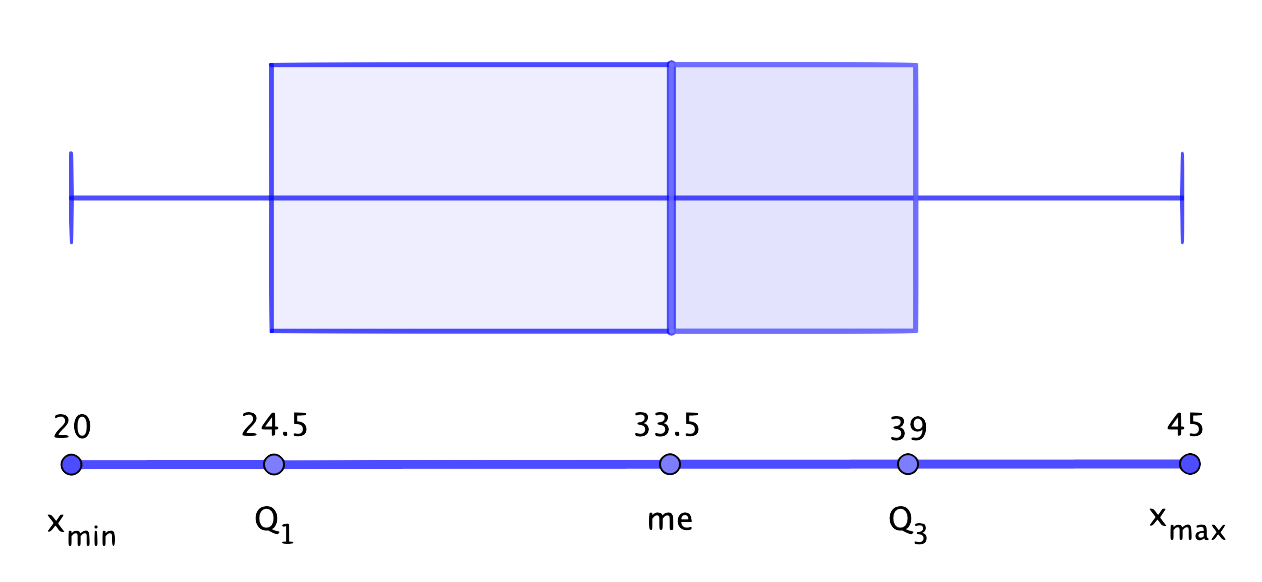
\includegraphics[width=.65\textwidth]{imagenes/imagenes01/T01IM15.png}
	\end{figure}
	
	\vspace{2mm} Algunas de las informaciones que se desprenden de la observación de este gráfico son:
	
	\vspace{1mm} --- La parte izquierda de la caja es mayor que la derecha. Los más jóvenes, entre el 25\% y el 50\% de la población tienen edades más dispersas que los mayores de entre el 50\% y 75\% de la población.
	
	\vspace{1mm} --- El bigote de la izquierda es menor que el de la derecha. El 25\% de los más jóvenes están más concentrados qu el 25\% de los más mayores.
	
	\vspace{1mm} --- El \emph{rango intercuartílico}, $Q_3-Q_1=$14.5. El 50\% de la población tiene edades que se diferencian en menos de 14.5 años.
	
	\vspace{1mm} --- La $me=$33,5. El 50\% de la población son. menores de 33.5 años y el otro 50\% tiene edades mayores a 33.5 años.
	
	\vspace{2mm} Además, los diagramas de cajas y bigotes son muy útiles para comparar dos distribuciones: supongamos otra distribución por edades de 20 personas cuyas edades son, 35, 38, 32, 28, 30, 29, 27, 19, 48, 40, 39, 24, 24, 34, 26, 41, 29, 48, 28, 22.
	
	\vspace{2mm} Los valores que ahora se obtienen son: $Q_1=26.5$, $Q_3=38.5$, $me=29.5$, $x_{min}=19$, $x_{max}=48$. Comparando ambos diagramas:
	
	\vspace{2mm} Ahora, puede obtenerse información respecto a las dos distribuciones.
	 
	 \begin{figure}[H]
			\centering
			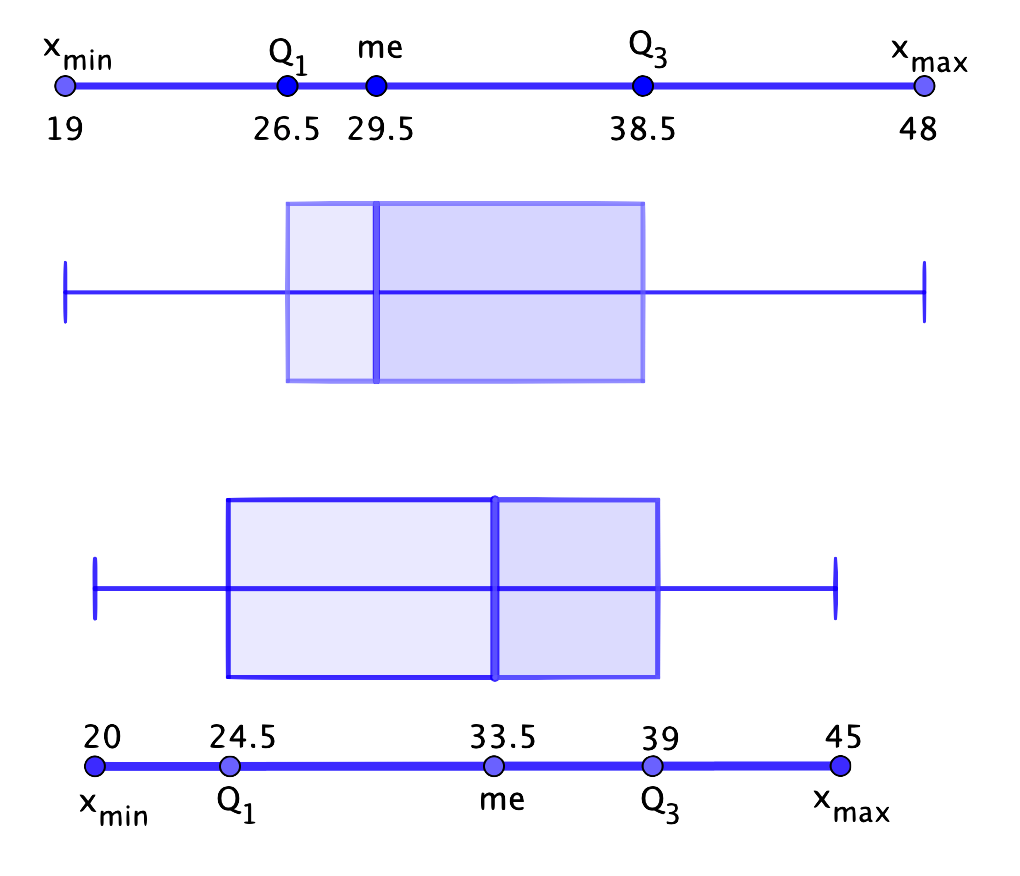
\includegraphics[width=.65\textwidth]{imagenes/imagenes01/T01IM16.png}
	\end{figure}
	
	\vspace{1mm} --- Rápidamente se observa que la segunda distribución, representada por el diagrama de cajas y bigotes de arriba, está más concentrada en edades que la representada abajo que es más dispersa (distribución primera). 
	
	\vspace{1mm} --- En la distribución de abajo (primera distribución), los datos eran más dispersos entre el 25\% y 50\% de la población. En la distribución de arriba (segunda distribución), ocurre al revés, los datos son más dispersos entre el 50\% y el 75\% de la población.
	
	\vspace{1mm} --- En cuanto a los bigotes, para la distribución de arriba se observa que son más largos, sobre todo la rama derecha lo cual indica que el 25\% de la población de esta distribución es más dispersa que la otra.
	
	\vspace{2mm} También se suelen representar en los diagramas de cajas y bigotes los llamados \emph{Valores atípicos} son aquellos que muestran una gran distancia a la mediana del resto de puntuaciones en la variable, es decir, o son demasiado bajas o son demasiado altas.  Numéricamente, se consideran \emph{valores atípicos} aquellos que sean menores que $Lim_{inf}=Q_1-1.5\cdot (Q_3-Q_1)$ o mayores que $Lim_{sup}=Q_3+1.5\cdot (Q_3-Q_1)$, de otro modo, los que están fuera del intervalo $(Lin_{inf},Lim_{sup})$, es decir, los que se separan de los cuartiles más de 1.5 veces el rango intercuartílico ($Q_3-Q_1$), 
	
	\vspace{2mm} 
	
\end{myalertblock}

\vspace{5mm}%**********************
\begin{myalertblock}{Relación entre media, mediana y moda.}

\begin{itemize}
\item si $\bar{x}=me=mo$, la distribución es \emph{simétrica}.
\item si $me>\bar{x}$, la distribución es \emph{asimétrica}, con cola a la derecha (\emph{sesgada a la derecha}).
\item si $me<\bar{x}$, la distribución es \emph{asimétrica}, con cola a la izquierda (\emph{sesgada a la izquierda}).
\end{itemize}

	 \begin{figure}[H]
			\centering
			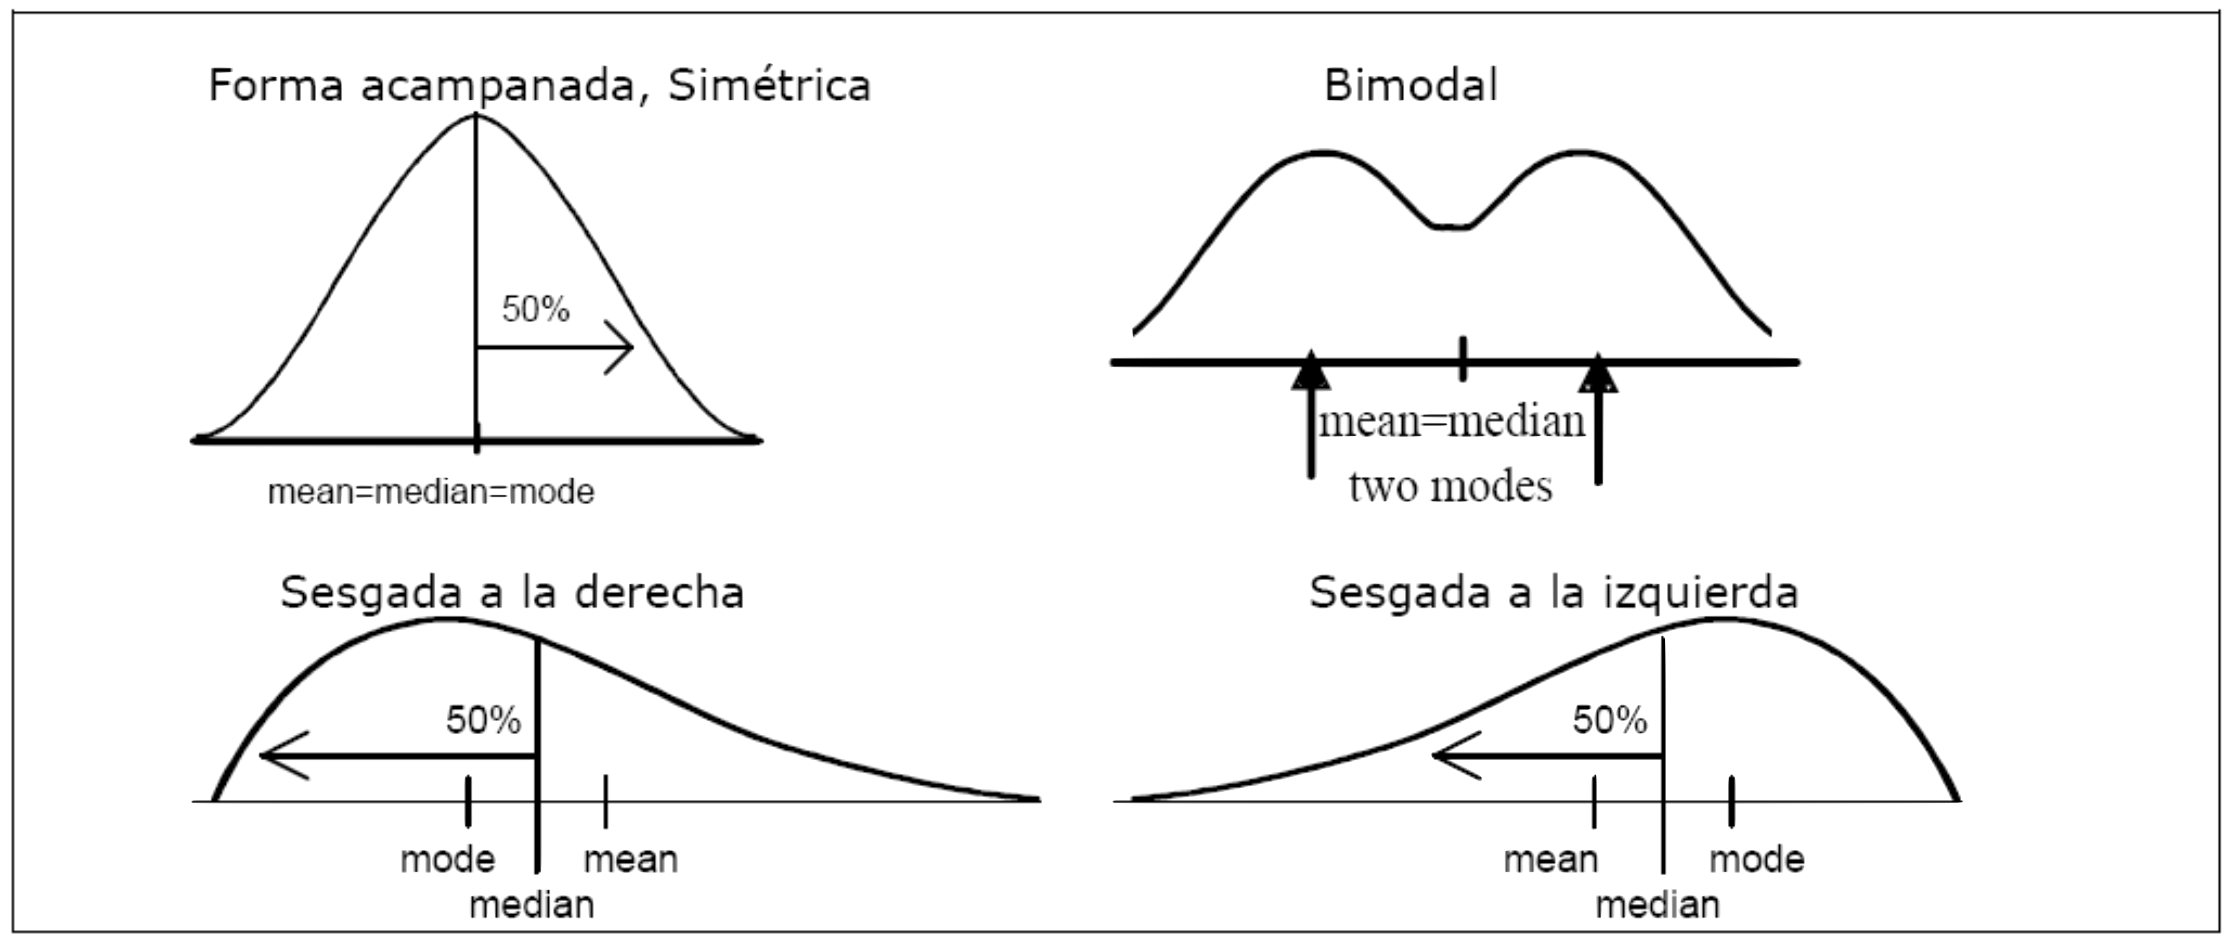
\includegraphics[width=1\textwidth]{imagenes/imagenes01/T01IM17.png}
	\end{figure}
	
\end{myalertblock}


\subsection{Parámetros de dispersión}
	
	Las medidas de dispersión, o de variabilidad (o propagación), expresan cómo se distribuyen los datos en torno a alguna de las medidas de centralización definidas antes (nos informan sobre cuánto se alejan del centro los valores de la distribución) y son un complemento a estas últimas para describir más fielmente un conjunto de datos.
	
	Cuanto más pequeña sea la medida de dispersión, mayor grado de agrupamiento de los datos respecto a la medida de centralización considerada (generalmente la media) y más representativa será este parámetro de centralización para definir el comportamiento de la distribución.
	
	Son de medidas de dispersión estadística son la varianza, la desviación típica, desviación media, el rango y rango intercuartílico. 
	
\vspace{5mm}%**********************
\begin{definition}
	. Se define el \textbf{recorrido} o 	\textbf{rango} de la distribución como la diferencia entre los valores mayor y menor de la variable.
	
	$$\boldsymbol{R\ = \ x_{max}-x_{min}}$$
	
	 Se define	el \textbf{rango intercuartílico} como la diferencia entre el tercer y el primer cuartil. Proporciona la longitud del intervalo en el que se encuentra el 50\% de las observaciones centrales.
	 
	 $$\boldsymbol{R_I\ =\ Q_3-Q_1}$$
\end{definition}

\vspace{5mm}%**********************
\begin{definition}
	. Se llama \textbf{desviación media} respecto al valor medio a la media de los valores absolutos de las diferencias de cada valor respecto del valor medio:
	
	$$\boldsymbol{ DM \ = \ \dfrac { \displaystyle \sum_{i=1}^n |x_i-\bar x|\cdot n_i }{N}  }$$	
\end{definition}

\vspace{5mm}%**********************
\begin{definition}
	. \textbf{Varianza, $\boldsymbol{s^2}$ y desviación típica, $\boldsymbol{s}$}. La desviación típica es la medida de dispersión más utilizada, representa la dispersión de los datos de la distribución respecto del valor medio y se expresa en sus mismas unidades.	
	
	$$\boldsymbol{ s^2=\dfrac {\displaystyle \sum_{i=1}^n (x_i-\bar x)^2\cdot n_i}{N}\ ; \qquad  \qquad \qquad s\ = \ \sqrt{s^2}}$$
\end{definition}

\vspace{5mm}%**********************	
\begin{theorem}
	. \begin{itemize}
 \item La varianza será siempre un valor positivo o cero (si todos los datos son iguales).

 \item Si a todos los valores de la variable se les suma un número la varianza no varía.

 $\{x_i\}\to s^2 \Rightarrow  \{x_i+d\}\to s^2$

\item Si todos los valores de la variable se multiplican por un número la varianza queda multiplicada por el cuadrado de dicho número.

 $\{x_i\}\to s^2 \Rightarrow \{ax_i\}\to a^2s^2$

\item Si tenemos varias distribuciones con la misma media y conocemos sus respectivas varianzas se puede calcular la varianza total.	

Para $n$ muestras de varianza $s_i^2$ formadas cada una de ellas por $k_i$ datos, la varianza total de la nueva distribución de $k_1+\cdots +k_n$ datos es:  $\ s^2=\dfrac {k_1 s_1^2+\cdots +k_n s_n^2}{k_1+\cdots +k_n}$

\item  Las siguientes definiciones de la varianza son equivalentes:

$$\subrayado{ \ \boxed{\ \boldsymbol{ s^2=\dfrac {\displaystyle \sum_{i=1}^n (x_i-\bar x)^2\cdot n_i}{N} \quad \leftrightarrow \quad s^2=\dfrac {\displaystyle \sum_{i=1}^n (x_i)^2\cdot n_i}{N}-{\bar {x}}^2  }\ } \ }$$
 \end{itemize}
	
\end{theorem}
	
\begin{proof}.

$s^2=\dfrac {\displaystyle \sum_{i=1}^n (x_i-\bar x)^2\cdot n_i}{N} =\dfrac {\displaystyle \sum_{i=1}^n (x_i^2-2x_i\bar x+{\bar x}^2)\cdot n_i}{N}=$

$=\dfrac {\displaystyle \sum_{i=1}^n x_i^2 \cdot n_i}{N}-2\bar x \dfrac{\displaystyle \sum_{i=1}^n x_i\cdot n_i}{N}+{\bar x}^2=
\dfrac {\displaystyle \sum_{i=1}^n x_i^2 \cdot n_i}{N} -2{\bar x}^2+{\bar x}^2=\dfrac {\displaystyle \sum_{i=1}^n x_i^2 \cdot n_i}{N}-{\bar x}^2$
\end{proof}

\textbf{Observaciones respecto a la varianza:}

\begin{enumerate}[1. ]
\item La varianza, al igual que la media, es un índice muy sensible a las puntuaciones extremas.
 
\item En los casos que no se pueda hallar la media tampoco será posible hallar la varianza.
\end{enumerate}

\vspace{5mm}%**********************
\begin{definition}
. El \textbf{coeficiente de variación}, también denominado como \emph{coeficiente de variación de Pearson}, es una medida estadística adimensional que nos informa acerca de la \underline{dispersión relativa} de varias distribuciones.	

\vspace{2mm} Si los valores sean positivos y su media dé, por tanto, un valor positivo, \emph{a mayor valor del coeficiente de variación mayor heterogeneidad (dispersión) de los valores de la variable}; y a \\emph{menor C.V., mayor homogeneidad (menor dispersión) en los valores de la variable}. Por ejemplo, si el C.V es menor o igual al 80\%, significa que la media aritmética es representativa del conjunto de datos, por ende el conjunto de datos es \emph{``Homogéneo''}. Por el contrario, si el C.V supera al 80\%, el promedio no será representativo del conjunto de datos (por lo que resultará \emph{``Heterogéneo''}). 

\vspace{2mm} El coeficiente de variación se define como la razón entre la desviación típica y el valor medio:

$$\boldsymbol{ CV \ = \ 	\dfrac {s}{\bar x}} \qquad \qquad\textcolor{gris}{(\bar x \neq 0})$$
\end{definition}

\vspace{5mm}%**********************
\begin{ejemplo}
\begin{ejre} Calcula las medidas de dispersión para la siguiente distribución estadística.
			
\begin{table}[H]
\centering
\begin{tabular}{r|r|r|r|r|r|r|}
\hline
\multicolumn{1}{|c|}{\textbf{$x_i$}} & \multicolumn{1}{c|}{\textbf{$n_i$}} & \multicolumn{1}{c|}{\textbf{$N_i$}} & \multicolumn{1}{c|}{\textbf{$x_i\cdot n_i$}} & \multicolumn{1}{c|}{\textbf{$x_i^2 \cdot n_i$}} & \multicolumn{1}{c|}{\textbf{$|x_i- \bar x|$}} & \multicolumn{1}{c|}{\textbf{$|x_i-\bar x| \cdot n_i$}} \\ \hline
\multicolumn{1}{|r|}{1} & 7 & 7 & 7 & 7 & 1.6 & 11.2 \\
\multicolumn{1}{|r|}{2} & 14 & 21 & 18 & 56 & 0.6 & 8.4 \\
\multicolumn{1}{|r|}{3} & 9 & 30 & 27 & 81 & 0.4 & 3.6 \\
\multicolumn{1}{|r|}{4} & 8 & 38 & 32 & 128 & 1.4 & 11.2 \\
\multicolumn{1}{|r|}{5} & 2 & 40 & 10 & 50 & 2.4 & 4.8 \\ \hline
 & \multicolumn{1}{c|}{N=40} &  & \multicolumn{1}{c|}{Total: 104} & \multicolumn{1}{c|}{Total: 322} &  & \multicolumn{1}{c|}{Total: 39.2} \\ \cline{2-2} \cline{4-5} \cline{7-7} 
\end{tabular}
\end{table}



--- Rango: $\ R=x_{max}-x_{min}=5.1=4$



--- Rango: $\ R=x_{max}-x_{min}=5.1=4$

$25\% (40)=10 \to Q_1=2; \quad 75\%(40)=30 \to Q_3=\dfrac{3+4}{5}=3.5$

--- Recorrido intercuartílico: $\ R_I=Q_3-Q_1=3.5-2=1.5$

$\bar x=\dfrac {\displaystyle \sum x_i \cdot n_i}{N}=\dfrac{104}{40}=2.6$

--- Desviación media: $\ DM  =  \dfrac { \displaystyle \sum_{i=1}^n |x_i-\bar x|\cdot n_i }{N}=\dfrac{39.2}{40}=0.98$ 

--- Varianza: $\ s^2 =\dfrac {\displaystyle \sum_{i=1}^n (x_i)^2\cdot n_i}{N}-{\bar {x}}^2=\dfrac{332}{40}-2.6^2=1.29$

--- Desviación típica: $\ s=\sqrt{s^2}=\sqrt{1.29}=1.14$

--- Coeficiente de variación (de Perason): $CV=\dfrac{s}{\bar x}=\dfrac{1.14}{2.6}=0.44=44 \%$

Si los datos estuviesen agrupados en intervalos, procederíamos de la misma forma, considerando como $x_i$ las marcas de clase.

\end{ejre}
\end{ejemplo}	
	
	
\vspace{5mm}%**********************	
\begin{ejemplo}
\begin{ejre} El cóndor de los Andes tiene una envergadura media (alas extendidas) de $285 \ \mathrm{cm}$ con una desviación estándar de $30 \ \mathrm{cm}$, mientras que una especie de murciélago tiene una envergadura media de $10 \ \mathrm{cm}$ y su población presenta una desviación estándar de $3 \ \mathrm{cm}$.

?`Cuál de las dos poblaciones presenta una mayor dispersión en lo que se refiere a su envergadura?	

\vspace{4mm} Condor: $\ CV=\dfrac{s}{\bar x}=\dfrac{30}{285}=0.11=11\%$

Murciélago: $\ CV=\dfrac{s}{\bar x}=\dfrac{3}{10}=0.30=30\%$

Aunque la desviación típica de la envergadura del cóndor de los Andes es muy superior a la de esa especie de murciélago, su dispersión es menor.
\end{ejre}
\end{ejemplo}

\subsection{Parámetros de forma}

Se usan para describir numéricamente la forma de la distribución. Miden la \emph{simetría} o sesgo y la \emph{curtosis} o apuntamiento y son parámetros adimensionales.

\vspace{5mm}%**********************
\begin{definition}
	. \textbf{Índices de asimetría}:
	
	
	\vspace{2mm} --- Coeficiente de asimetría de Fisher: $\ As=\dfrac{\displaystyle \sum_{i=1}^n (x_i-\bar x)^3 \ n_i}{N s^3}$
	
	\vspace{4mm} Interpretación de los coeficientes: Si $As>0$ la distribución presenta una asimetría positiva, si $As<0$ la asimetría es negativa y si $As\simeq 0$ la distribución es simétrica.
	
	\begin{figure}[H]
			\centering
			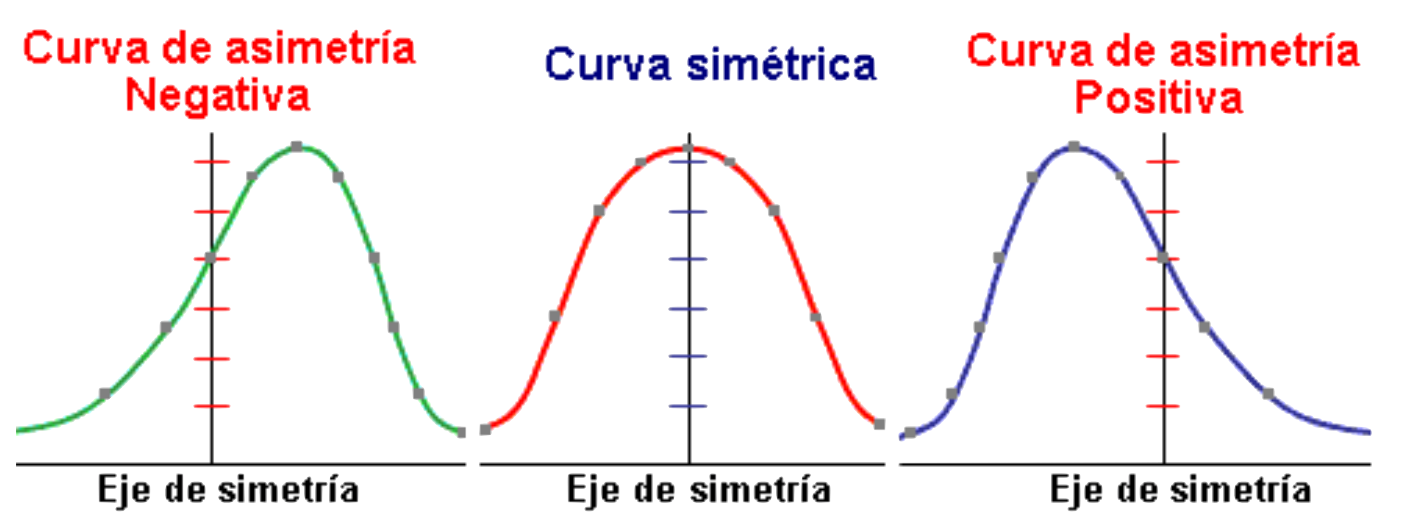
\includegraphics[width=.75\textwidth]{imagenes/imagenes01/T01IM18.png}
	\end{figure}
\end{definition}

\vspace{5mm}%**********************	
\begin{definition}
	. El \textbf{apuntamiento o curtosis} proviene de una comparación de la distribución con la \emph{distribución normal o campana de Gauss} por lo que solo tendrá sentido para las distribuciones que se asemejen a la curva normal (unimodales y prácticamente simétricas). Para su medida se usa el
	
	\vspace{2mm} --- Coeficiente de apuntamiento de Fisher: $\ K=\dfrac{\displaystyle \sum_{i=1}^n (x_i-\bar x)^4 \ n_i}{Ns^4}-3$
	
	\vspace{4mm} Si $K<0$ tenemos una distribución \emph{platicúrtica}, en las colas de la distribución hay más casos que en la curva normal. Si $K>0$ la distribución es \emph{leptocúrtica}, ocurre lo contrario que en el caso anterior. Para $K\simeq 0$ la distribución es como la normal, se llama \emph{mesocúrtica}.
	
	\begin{figure}[H]
			\centering
			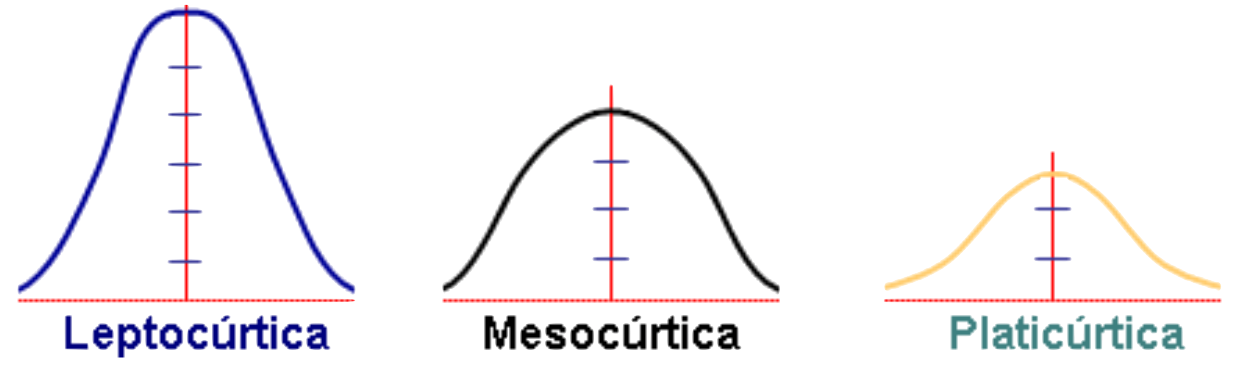
\includegraphics[width=.75\textwidth]{imagenes/imagenes01/T01IM19.png}
	\end{figure}
	
	\end{definition}

\vspace{5mm}%**********************
\begin{example}
	. Calcula el coeficiente de asimetría y la curtosis para la siguiente distribución.
	
	\begin{figure}[H]
			\centering
			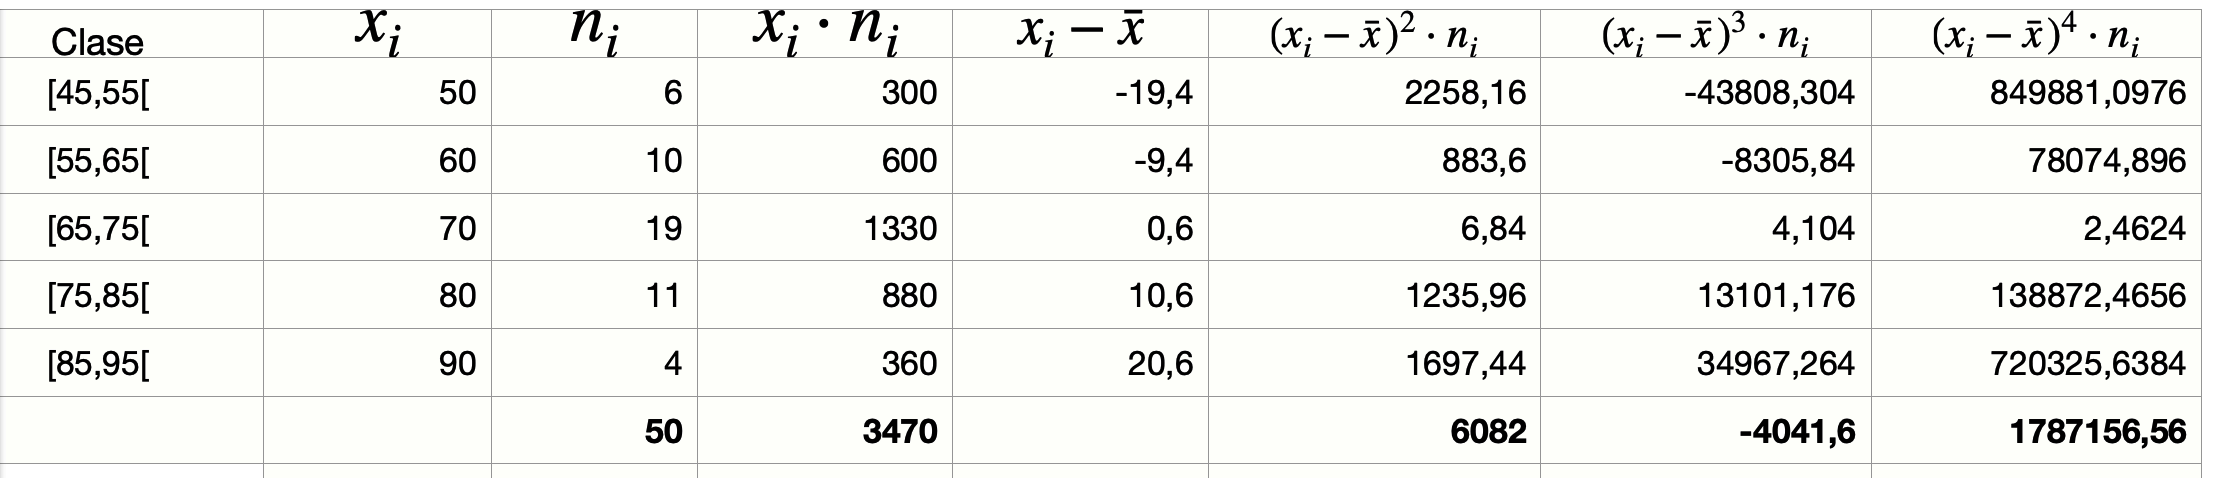
\includegraphics[width=1\textwidth]{imagenes/imagenes01/T01IM20.png}
	\end{figure}
	
	
	$\bar x=\dfrac{3470}{50}=69.4$ $;\qquad$ $\sigma=\sqrt{\dfrac{6082}{50}}=11.0$
	
	$As=\dfrac{-4041.6}{50\cdot 11.0^3}=-0.06\simeq -0.1$
	
	$K=\dfrac{1787156.56}{50\cdot 11.0^4}-3=2.4-3=-0.6$	
	

\vspace{2mm}La distribución es prácticamente simétrica (ligero sesgo o asimetría negativa o hacia la izquierda) y platicúrtica.
		
\end{example}

\subsection{Interpretación conjunta de la media y la desviación típica}
\label{mediaydesviacion}
	
\begin{myalertblock}{$\boldsymbol{ \bar x \ \text{ y } \ \sigma. }$}
	Cuando la distribución en estudio es \emph{``normal''} (de momento no sabemos que significa esto de 'normal' -- lo veremos en distribuciones de probabilidad -- pero supongamos que son aquellas que no presentan valores `extraños') resulta que datos de la distribución que se alejen una desviación típica del valor medio hay alrededor de los 2/3 del total de datos, es decir, individuos con $x_i\in[\bar x -\sigma, \bar x+\sigma]$ son aproximadamente el $68\%$ del total. Los que se alejan dos desviaciones típicas son el $95\%$ del total y tres desviaciones típicas el $99.7\%$.
	
	\begin{figure}[H]
			\centering
			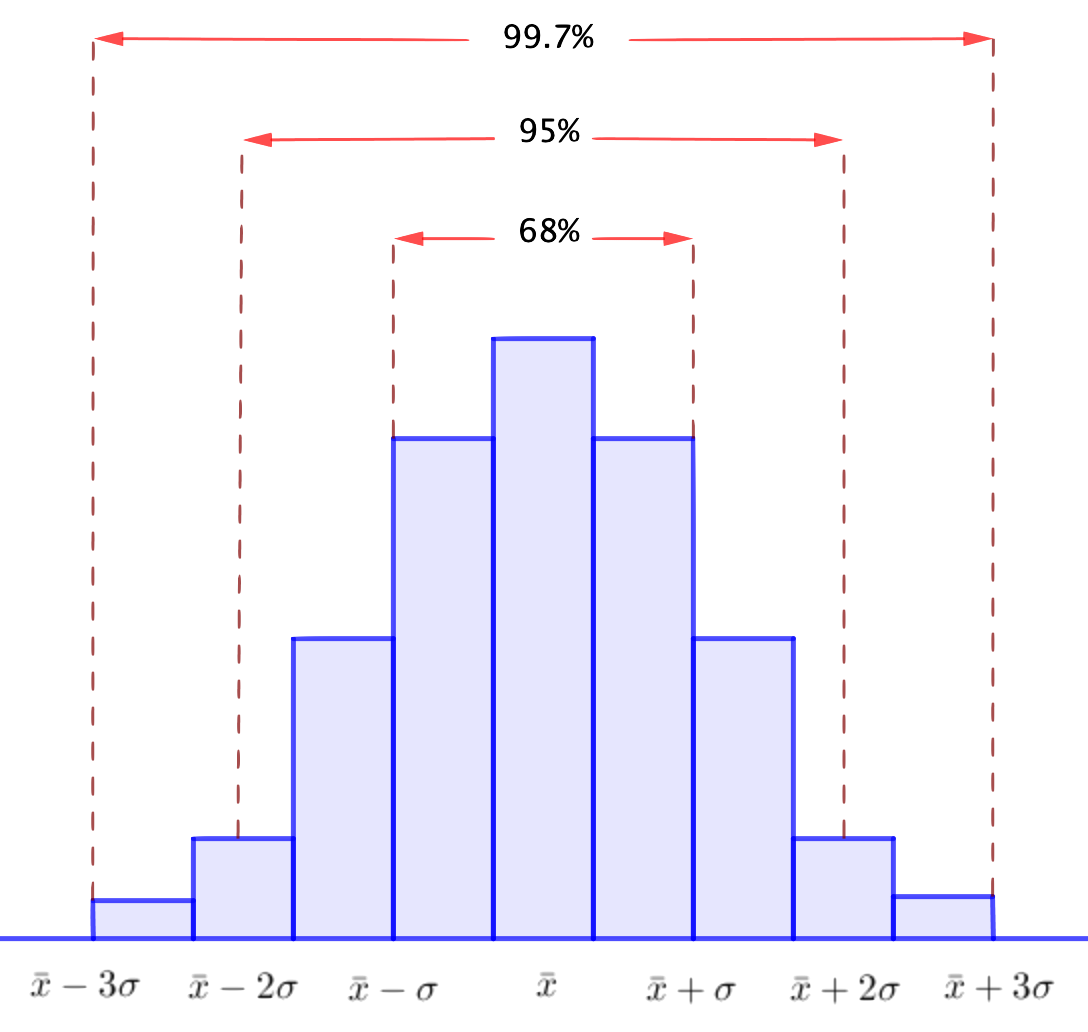
\includegraphics[width=.7\textwidth]{imagenes/imagenes01/T01IM21.png}
	\end{figure}
\end{myalertblock}

\section{Tipificación}

\begin{definition}
	
Haciendo uso de las propiedades de las medidas estadísticas, podremos facilitar y simplificar los cálculos de parámetros estadísticos mediante un cambio de variable.

\vspace{2mm} Así, si todos los valores son muy altos, podremos restarles una cantidad (normalmente la Moda) y, si poseen cifras decimales o son múltiplos de un mismo número, podremos multiplicarlos o dividirlos por el valor adecuado. 

\vspace{2mm} Una vez calculados los parámetros estadísticos, en virtud de las propiedades descritas, obtendremos el valor final real de tales parámetros. 

\vspace{2mm} Mención especial merecen dos cambio de variables particular : 

1.$\ $ \textbf{Diferenciales}: partiendo de la variable inicial $x_i$ (puntuaciones directas), si a todos los valores les restamos la media, obtenemos una nueva variable $y_i=x_i-\var x$ (puntuaciones diferenciales) cuya media es cero (la desviación típica no se modifica). 

2.$\ $  \textbf{Tipificadas}: Si a todos los valores de la variable inicial $x_i$ les restamos la media y el resultado lo dividimos por la desviación típica, obtenemos una nueva variable $\boldsymbol{z_i=\frac{x_i-\bar x}{s_x}}$, \emph{puntuaciones típicas o tipificadas} cuya media es cero y cuya  desviación típica es siempre la unidad. 

\vspace{2mm} Este último cambio de variable recibe el nombre de \textbf{TIPIFICACIÓN} y es muy útil a la hora de comparar dos valores de individuos pertenecientes a distribuciones distintas.
\end{definition}

\vspace{15mm}%**********************
\begin{example}

Un alumno obtiene en un examen de matemáticas una calificación de $8$ en un grupo cuya media es $5$ y desviación típica $1$. Su amigo, en otro grupo de media $6$ y desviación típica $2$ obtiene un $10$. ?`Cuál de las dos notas, comparativamente a su grupo, es mejor calificación?. 

\vspace{4mm} Nos encontramos con dos distribuciones de calificaciones medidas en distintas escalas. Para poder comparar tendremos que referir ambas series de valores a otras equivalentes entre sí (igual media y desviación típica). 

\vspace{2mm} El proceso de \emph{tipificación} nos proporciona lo que deseamos, siempre obtendremos una distribución con media $0$ y desviación típica $1$, donde los datos ya son comparables.
 
\vspace{2mm} Tipificando ambas calificaciones se obtiene :

\vspace{2mm} Nota del primer amigo: $\ z_i=\dfrac{8-5}{1}=3$

\vspace{2mm} Nota del segundo amigo: $z_2=\dfrac{10-6}{2}=2$ 

\vspace{2mm} La nota obtenida del primer amigo es, comparativamente,  superior a la del segundo. 
\end{example}

\newpage %********************************************
\section{Ejercicios}
	
\begin{ejemplo}
\begin{ejer}
	Considera las siguientes distribuciones:
	
\begin{table}[H]
\centering
\begin{tabular}{|r|r|r|r|r|}
\cline{1-2} \cline{4-5}
\multicolumn{2}{|c|}{\textbf{Distribución 1}} & \multicolumn{1}{c|}{\textbf{}} & \multicolumn{2}{c|}{\textbf{Distribución 2}} \\ \cline{1-2} \cline{4-5} 
\multicolumn{1}{|c|}{\textbf{clase}} & \multicolumn{1}{c|}{\textbf{$n_i$}} & \multicolumn{1}{c|}{\textbf{$\qquad$}} & \multicolumn{1}{c|}{\textbf{clase}} & \multicolumn{1}{c|}{\textbf{$n_i$}} \\ \cline{1-2} \cline{4-5} 
[10,20[ & 3 &  & [10,20[ & 5 \\ \cline{1-2} \cline{4-5} 
[20,30[ & 17 &  & [20,30[ & 9 \\ \cline{1-2} \cline{4-5} 
[30,40[ & 13 &  & [30,40[ & 23 \\ \cline{1-2} \cline{4-5} 
[40,50[ & 9 &  & [40,50[ & 9 \\ \cline{1-2} \cline{4-5} 
[50,60[ & 8 &  & [50,60[ & 4 \\ \cline{1-2} \cline{4-5} 
\end{tabular}
\end{table}	
\end{ejer}

$a)\quad$ Dibuja el histograma de cada distribución y deduce, de su observación, cuál de las dos distribuciones es más dispersa.

$b)\quad$ Calcula $mo, \ me, \ Q_1, D_1, P_{66}$ para la primera distribución.

$c)\quad$ Calcula $\bar x,\ \bar x_g, \bar x_a$ para la primera distribución.

$d)\quad$ Calcula el rango, la desviación media y la desviación típica, para la primera distribución.

$e)\quad$ Calcula los coeficientes de variación de Pearson para ambas distribuciones y deduce, a partir de ellos, cuál es la distribución más dispersa.

$f)\quad$ Da, para la primera distribución, una interpretación conjunta de media y desviación típica. ?`A partir de qué valor se está entre los 10\% valores más altos? ?`Cuántos valores hay menores que 47? 

$g)\quad$ Encuentra los coeficientes de asimetría y de curtosis de ambas distribuciones. ?`Qué puedes decir de la forma de estas distribuciones?.

$h)\quad$ Dibuja el diagrama de cajas y bigotes.

$i)\quad$ ?`Entre que valores se encuentra el 20\% de los valores centrales?

\end{ejemplo}

Cálculos:


\begin{table}[H]
\tiny
\centering
\begin{tabular}{rrrrrrrrr}
\multicolumn{8}{l}{\textbf{Distribución 1}} & \multicolumn{1}{l}{\textbf{}} \\ \hline
\multicolumn{1}{|c|}{\textbf{$x_i$}} & \multicolumn{1}{c|}{\textbf{$n_i$}} & \multicolumn{1}{c|}{\textbf{$N_i$}} & \multicolumn{1}{c|}{\textbf{$x_i \cdot n_i$}} & \multicolumn{1}{c|}{\textbf{$x_i-\bar x$}} & \multicolumn{1}{c|}{\textbf{$|x_i-\bar x|\cdot n_i$}} & \multicolumn{1}{c|}{\textbf{$(x_i-\bar x)^2\cdot n_i$}} & \multicolumn{1}{c|}{\textbf{$(x_i-\bar x)^3\cdot n_i$}} & \multicolumn{1}{c|}{\textbf{$(x_i-\bar x)^4\cdot n_i$}} \\ \hline
\multicolumn{1}{|r|}{15} & \multicolumn{1}{r|}{3} & \multicolumn{1}{r|}{3} & \multicolumn{1}{r|}{45} & \multicolumn{1}{r|}{-20.4} & \multicolumn{1}{r|}{61.2} & \multicolumn{1}{r|}{1248.48} & \multicolumn{1}{r|}{-25468.99} & \multicolumn{1}{r|}{519567.44} \\ \hline
\multicolumn{1}{|r|}{25} & \multicolumn{1}{r|}{17} & \multicolumn{1}{r|}{20} & \multicolumn{1}{r|}{425} & \multicolumn{1}{r|}{-10.4} & \multicolumn{1}{r|}{176.8} & \multicolumn{1}{r|}{1838.72} & \multicolumn{1}{r|}{-19122.69} & \multicolumn{1}{r|}{198875.96} \\ \hline
\multicolumn{1}{|r|}{35} & \multicolumn{1}{r|}{13} & \multicolumn{1}{r|}{33} & \multicolumn{1}{r|}{455} & \multicolumn{1}{r|}{-0.4} & \multicolumn{1}{r|}{5.2} & \multicolumn{1}{r|}{2.08} & \multicolumn{1}{r|}{-0.83} & \multicolumn{1}{r|}{0.33} \\ \hline
\multicolumn{1}{|r|}{45} & \multicolumn{1}{r|}{9} & \multicolumn{1}{r|}{42} & \multicolumn{1}{r|}{405} & \multicolumn{1}{r|}{9.6} & \multicolumn{1}{r|}{86.4} & \multicolumn{1}{r|}{829.44} & \multicolumn{1}{r|}{7962.62} & \multicolumn{1}{r|}{76441.19} \\ \hline
\multicolumn{1}{|r|}{55} & \multicolumn{1}{r|}{8} & \multicolumn{1}{r|}{50} & \multicolumn{1}{r|}{440} & \multicolumn{1}{r|}{19.6} & \multicolumn{1}{r|}{156.8} & \multicolumn{1}{r|}{3073.28} & \multicolumn{1}{r|}{60236.29} & \multicolumn{1}{r|}{1180631.24} \\ \hline
\multicolumn{1}{r|}{\textbf{}} & \multicolumn{1}{r|}{\textbf{N=50}} & \multicolumn{1}{r|}{\textbf{}} & \multicolumn{1}{r|}{\textbf{1770}} & \multicolumn{1}{r|}{\textbf{}} & \multicolumn{1}{r|}{\textbf{486.4}} & \multicolumn{1}{r|}{\textbf{6992.00}} & \multicolumn{1}{r|}{\textbf{23606.40}} & \multicolumn{1}{r|}{\textbf{1975516.16}} \\ \cline{2-2} \cline{4-4} \cline{6-9} 
\end{tabular}
\end{table}

\begin{table}[H]
\tiny
\centering
\begin{tabular}{rrrrrrrrr}
\multicolumn{8}{l}{\textbf{Distribución 2}} & \multicolumn{1}{l}{\textbf{}} \\ \hline
\multicolumn{1}{|c|}{\textbf{$x_i$}} & \multicolumn{1}{c|}{\textbf{$n_i$}} & \multicolumn{1}{c|}{\textbf{$N_i$}} & \multicolumn{1}{c|}{\textbf{$x_i \cdot n_i$}} & \multicolumn{1}{c|}{\textbf{$x_i-\bar x$}} & \multicolumn{1}{c|}{\textbf{$|x_i-\bar x|\cdot n_i$}} & \multicolumn{1}{c|}{\textbf{$(x_i-\bar x)^2\cdot n_i$}} & \multicolumn{1}{c|}{\textbf{$(x_i-\bar x)^3\cdot n_i$}} & \multicolumn{1}{c|}{\textbf{$(x_i-\bar x)^4\cdot n_i$}} \\ \hline
\multicolumn{1}{|r|}{15} & \multicolumn{1}{r|}{5} & \multicolumn{1}{r|}{5} & \multicolumn{1}{r|}{75} & \multicolumn{1}{r|}{-19.6} & \multicolumn{1}{r|}{98} & \multicolumn{1}{r|}{1920.8} & \multicolumn{1}{r|}{-37647.68} & \multicolumn{1}{r|}{737894.53} \\ \hline
\multicolumn{1}{|r|}{25} & \multicolumn{1}{r|}{9} & \multicolumn{1}{r|}{14} & \multicolumn{1}{r|}{225} & \multicolumn{1}{r|}{-9.6} & \multicolumn{1}{r|}{86.4} & \multicolumn{1}{r|}{829.44} & \multicolumn{1}{r|}{-7962.62} & \multicolumn{1}{r|}{76441.19} \\ \hline
\multicolumn{1}{|r|}{35} & \multicolumn{1}{r|}{23} & \multicolumn{1}{r|}{37} & \multicolumn{1}{r|}{805} & \multicolumn{1}{r|}{0.4} & \multicolumn{1}{r|}{9.2} & \multicolumn{1}{r|}{3.68} & \multicolumn{1}{r|}{1.47} & \multicolumn{1}{r|}{0.59} \\ \hline
\multicolumn{1}{|r|}{45} & \multicolumn{1}{r|}{9} & \multicolumn{1}{r|}{46} & \multicolumn{1}{r|}{405} & \multicolumn{1}{r|}{10.4} & \multicolumn{1}{r|}{93.6} & \multicolumn{1}{r|}{973.44} & \multicolumn{1}{r|}{10123.78} & \multicolumn{1}{r|}{105287.27} \\ \hline
\multicolumn{1}{|r|}{55} & \multicolumn{1}{r|}{4} & \multicolumn{1}{r|}{50} & \multicolumn{1}{r|}{220} & \multicolumn{1}{r|}{20.4} & \multicolumn{1}{r|}{81.6} & \multicolumn{1}{r|}{1664.64} & \multicolumn{1}{r|}{33958.66} & \multicolumn{1}{r|}{692756.58} \\ \hline
\multicolumn{1}{r|}{\textbf{}} & \multicolumn{1}{r|}{\textbf{N=50}} & \multicolumn{1}{r|}{\textbf{}} & \multicolumn{1}{r|}{\textbf{1730}} & \multicolumn{1}{r|}{\textbf{}} & \multicolumn{1}{r|}{\textbf{368.8}} & \multicolumn{1}{r|}{\textbf{5392.00}} & \multicolumn{1}{r|}{\textbf{-1526.40}} & \multicolumn{1}{r|}{\textbf{1612380.16}} \\ \cline{2-2} \cline{4-4} \cline{6-9} 
\end{tabular}
\end{table}

Para el cálculo de las desviaciones es necesario, previamente, calcular la medias:

\vspace{-4mm}%***********************************
$$\bar x_1=\dfrac{1770}{50}=34,5; \qquad \bar x_2=\dfrac{1730}{50}=34,6$$

\textcolor{blue}{------ $a)\ $  Histogramas:}
\begin{figure}[H]
			\centering
			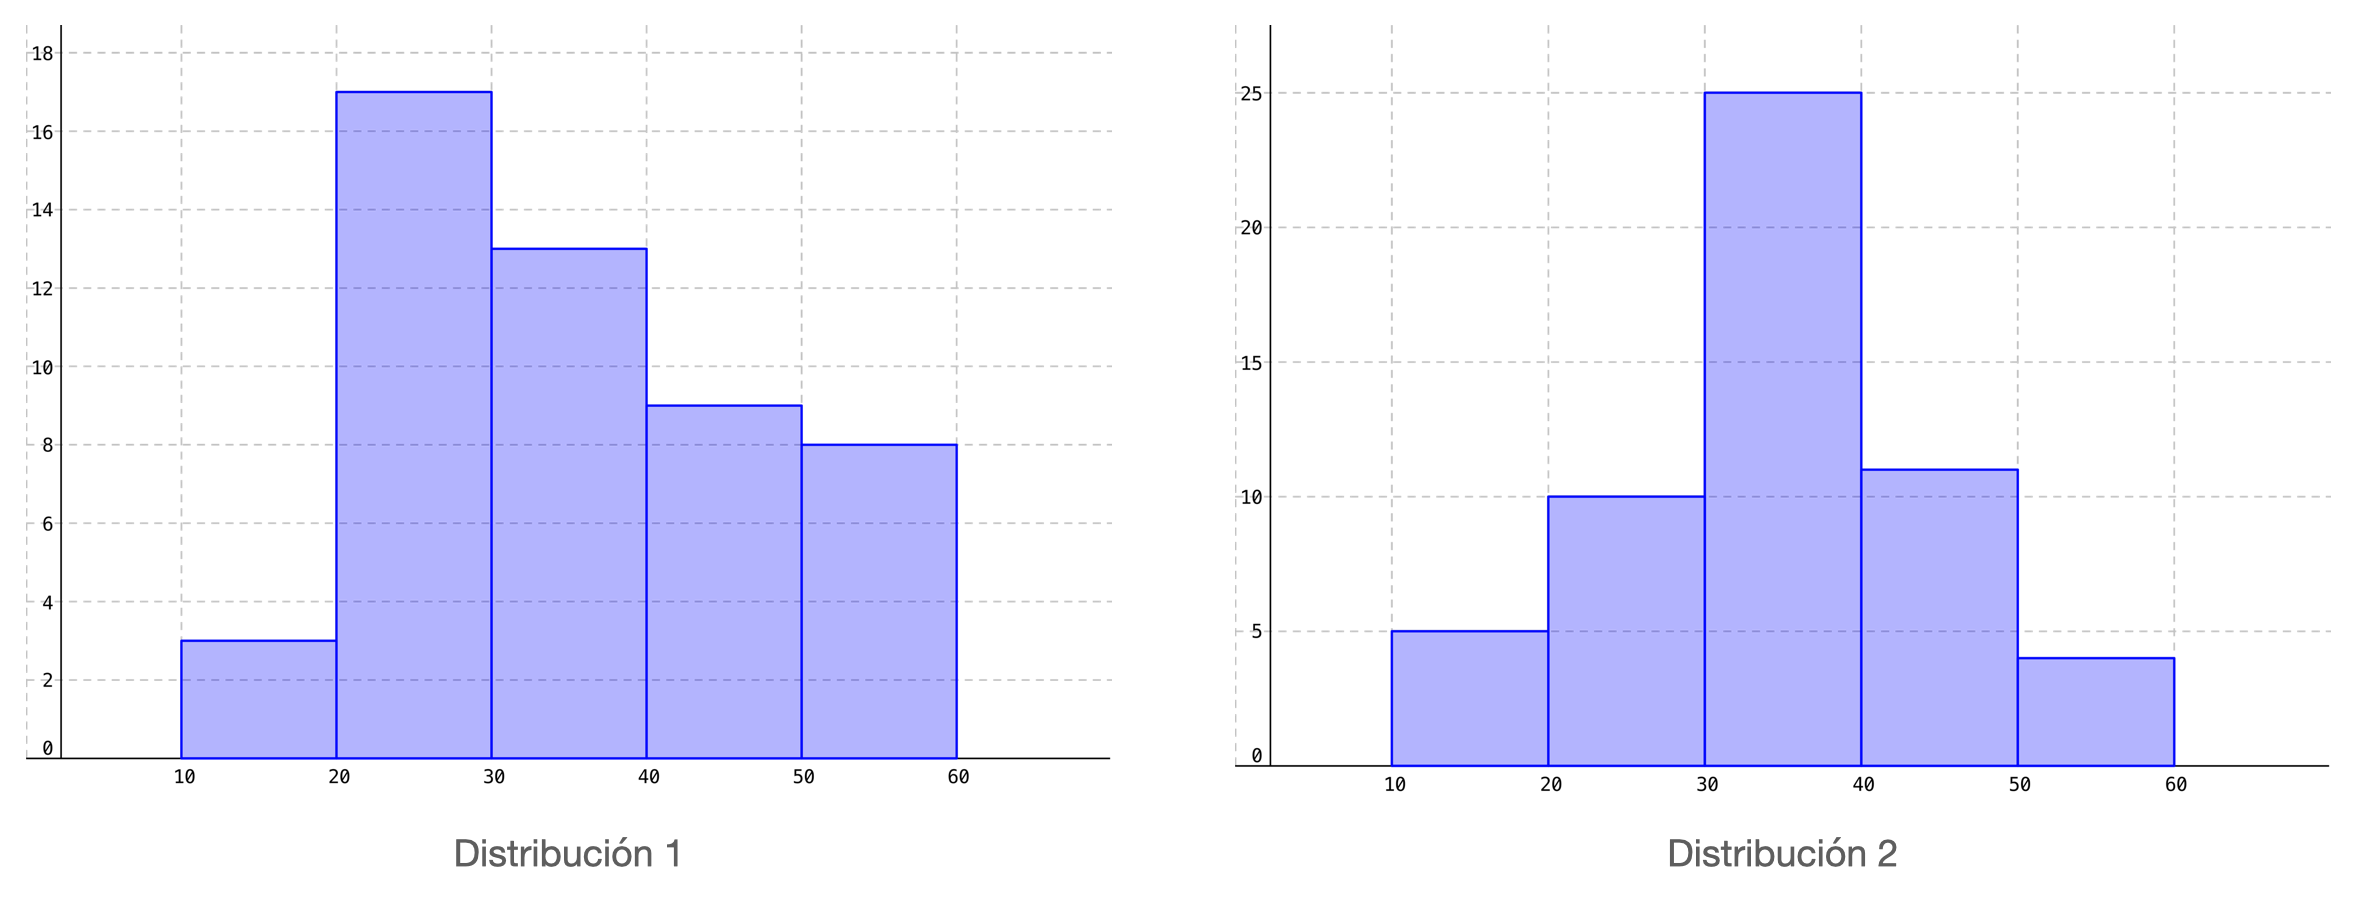
\includegraphics[width=.9\textwidth]{imagenes/imagenes01/T01IM22.png}
	\end{figure}


\vspace{-4mm} %******************************************
A simple vista, la distribución 1 parece más dispersa que la distribución 2. En el apartado $e)$ lo veremos con más precisión al calcular los respectivos coeficientes de variación (Pearson). 
	
\textcolor{blue}{------ $b)\  mo, me, Q_1, D_1, P_{66}$ para la primera distribución:}

El intervalo modal, de mayor frecuencia absoluta, es el $[20,30[$, su frecuencia absoluta es $n_k=17$ y las frecuencias absolutas de los intervalos anterior y posterior	son, respectivamente, $m_{k-1}=3$ y $n_{k+1}=13$. La amplitud del intervalo modal es $c_k=10$, como la de todos ellos.
	
$\Rightarrow \quad mo=20+\dfrac{17-3}{(17-3)+(17-13)}\ 10=27.8$

\vspace{5mm} %******************
{\color{gris}\hrule} 
\begin{multicols}{2}
Calculamos la moda sin usar la fórmula:

Los triángulos $AOB \sim DOE$ son \emph{semejantes}.

$\dfrac{AB}{OC}=\dfrac{DE}{OF}$

$\dfrac{14}{x}=\dfrac{4}{10-x}$

$x=7.8 \Rightarrow $



$\qquad mo=20+7.8=27.8$

\begin{figure}[H]
			\centering
			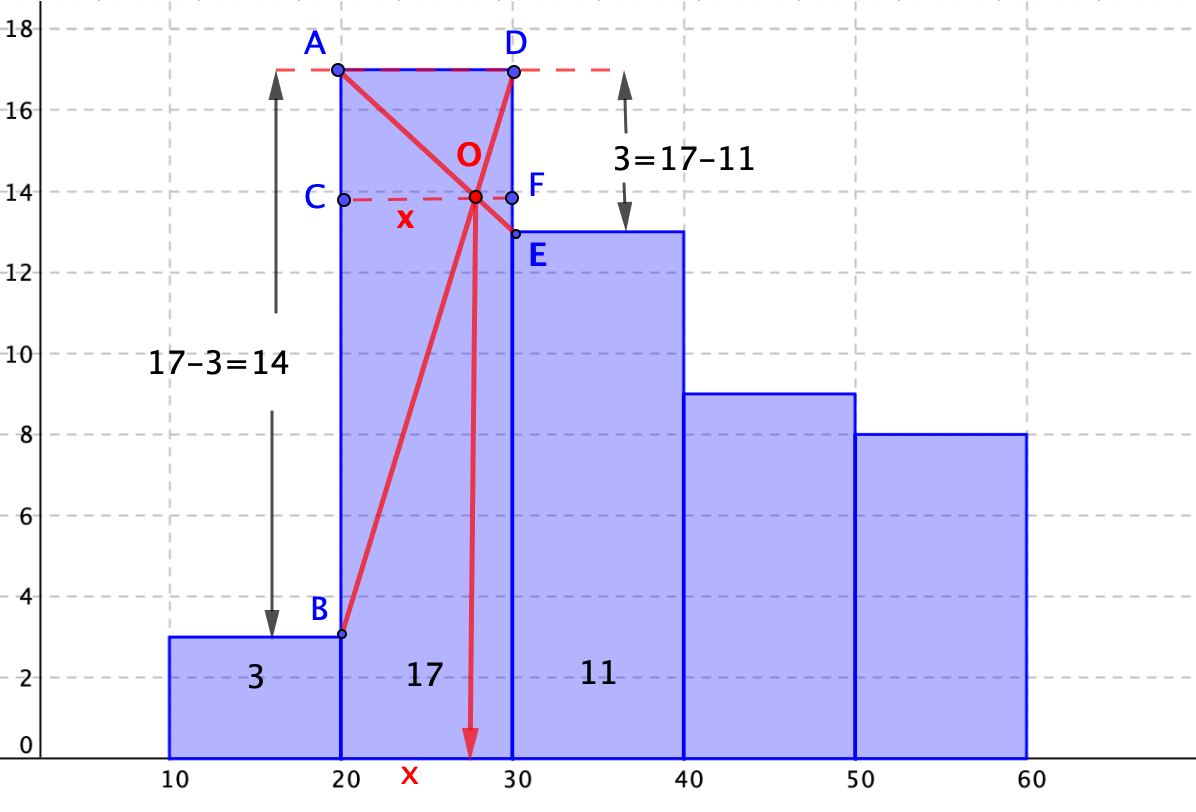
\includegraphics[width=.5\textwidth]{imagenes/imagenes01/T01IM23.png}
	\end{figure}
\end{multicols}
{\color{gris}\hrule}

\vspace{5mm} %*******************************
El intervalo mediano es el tercero, $[30,40[$ de frecuencia absoluta $n_k=13$ y cuya frecuencia acumulada del intervalo anterior es $N_{k-1}=20$. La amplitud de éste y todos los intervalos en $c_k=10$.

$\Rightarrow \quad  me=30+\dfrac{\dfrac{50}{2}-20}{13}\ 10=33.8$


\vspace{10mm}
{\color{gris}\hrule}
\begin{multicols}{2}
Calculamos la mediana sin usar la fórmula:

Los triángulos $AOB \sim ADC$ 

son \emph{semejantes}.

$\quad$

$\dfrac{OB}{AB}=\dfrac{DC}{AC}$

$\dfrac{5}{x}=\dfrac{13}{10}$

$x=3.8 \Rightarrow $

$\qquad  mo=30+3.8=33.8$

\begin{figure}[H]
			\centering
			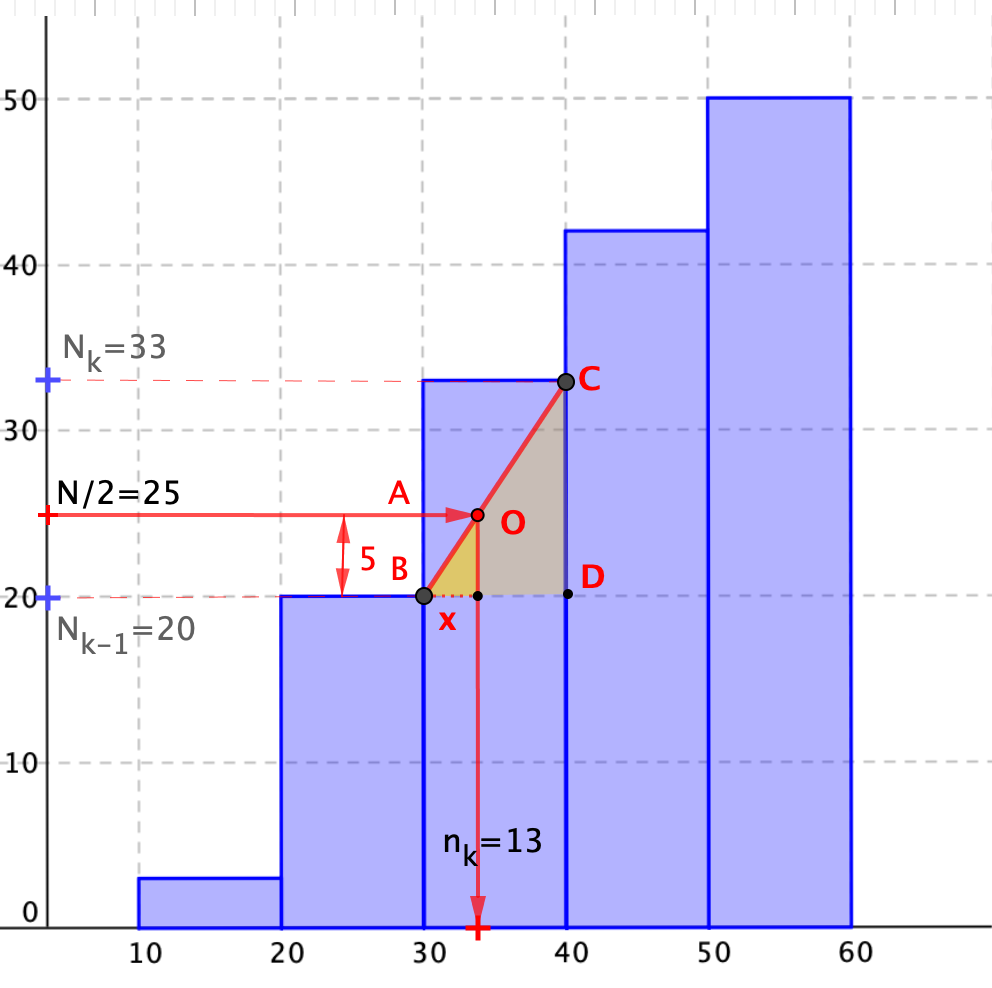
\includegraphics[width=.4\textwidth]{imagenes/imagenes01/T01IM24.png}
	\end{figure}
\end{multicols}

{\color{gris}\hrule}
	
\vspace{4mm} %*******************************

$\Rightarrow \quad  25\% (50)=12.5 \to Q_1=20+ \dfrac{12.5-3}{17}\ 10=25.6$

$\Rightarrow \quad 10\% (50)=5 \to D_1=20+\dfrac{5-3}{17}\ 10=21.2$

$\Rightarrow \quad 65\% (50)=32.5 \to P_{66}=30+\dfrac{32.5-20}{13}\ 10=39.6$

\textcolor{blue}{------ $c)\ \bar x,\ \bar x_g,\ \bar x_a$ de distribución-1.}

\begin{table}[H]
\footnotesize
\centering
\begin{tabular}{rrrrr}
\multicolumn{1}{l}{\textbf{Distribución 1}} & \multicolumn{1}{l}{\textbf{}} & \multicolumn{1}{l}{\textbf{}} & \multicolumn{1}{l}{\textbf{}} & \multicolumn{1}{l}{\textbf{}} \\ \hline
\multicolumn{1}{|c|}{\textbf{$x_i$}} & \multicolumn{1}{c|}{\textbf{$n_i$}} & \multicolumn{1}{c|}{\textbf{$x_i \cdot n_i$}} & \multicolumn{1}{c|}{\textbf{${x_i}^{n_i}$}} & \multicolumn{1}{c|}{\textbf{$n_i / x_i$}} \\ \hline
\multicolumn{1}{|r|}{15} & \multicolumn{1}{r|}{3} & \multicolumn{1}{r|}{45} & \multicolumn{1}{r|}{3.30E+03} & \multicolumn{1}{r|}{0.20} \\ \hline
\multicolumn{1}{|r|}{25} & \multicolumn{1}{r|}{17} & \multicolumn{1}{r|}{425} & \multicolumn{1}{r|}{5.82E+23} & \multicolumn{1}{r|}{0.68} \\ \hline
\multicolumn{1}{|r|}{35} & \multicolumn{1}{r|}{13} & \multicolumn{1}{r|}{455} & \multicolumn{1}{r|}{1.18E+20} & \multicolumn{1}{r|}{0.37} \\ \hline
\multicolumn{1}{|r|}{45} & \multicolumn{1}{r|}{9} & \multicolumn{1}{r|}{405} & \multicolumn{1}{r|}{7.57E+14} & \multicolumn{1}{r|}{0.20} \\ \hline
\multicolumn{1}{|r|}{55} & \multicolumn{1}{r|}{8} & \multicolumn{1}{r|}{440} & \multicolumn{1}{r|}{8.37E+13} & \multicolumn{1}{r|}{0.15} \\ \hline
\multicolumn{1}{r|}{\textbf{}} & \multicolumn{1}{r|}{\textbf{N=50}} & \multicolumn{1}{r|}{\textbf{1770}} & \multicolumn{1}{r|}{\textbf{$\Pi=\ $ 1.47E+76}} & \multicolumn{1}{r|}{\textbf{1.60}} \\ \cline{2-5} 
\end{tabular}
\end{table}

$\bar x=\dfrac {1770}{50}=35.4;\quad \bar x_g=\sqrt[50]{1.47\times 10^{76}}=33.4;\quad \bar x_a =\dfrac{50}{1.60}=31.3$

\textcolor{blue}{------ $d)\ R,\ DM,\ s$ ,  de distribución-1.}

$\Rightarrow \quad R=60-10=50$

$\Rightarrow \quad DM=\dfrac{486.4}{50}=9.7$

$\Rightarrow \quad s=\sqrt{\dfrac{6992.00}{50}}=11.83$

\textcolor{blue}{------ $e)\ $ CV para ambas distribuciones:}

$\bar x_1=35.5;\ \ s_1=11.83; \qquad x_2=34.6; \ \ s_2=\sqrt{\dfrac{5392}{50}}=10.38$

$\Rightarrow \quad CV_1=\dfrac{\bar s_1}{x_1}=0.343=34.3\%$

$\Rightarrow \quad CV_2=\dfrac{\bar s_2}{x_2}=0.300=30.0\%$

Como habíamos predicho en el apartado $\ a)\ $ la primera distribución tiene los datos más dispersos.

\textcolor{blue}{------ $f)\ n_i \in [\bar x-\sigma, \bar x+\sigma];\ \ \ 10\% \uparrow \to P_90; \ \ \ $ ?`cuantos individuos tiene $x_i<47$?.} 

En el intervalo $ [\bar x-\sigma, \bar x+\sigma]=[22.67,46,33]$ están todos los individuos del intervalo $[30,40[$, esto es, $\underline {13}$ individuos más la parte proporcional de individuos de cada uno de los intervalos adyacentes. 

En $[20,30[$ hay $17$ individuos, para una amplitud de $10$. En $[22.67,30[$, de amplitud $7.33$ habrán:  $17\ \frac{7.33}{10}=\underline{12.46}$

$\Rightarrow \quad $ En $[40,50[$ hay $9$ individuos, para una amplitud de $10$. En $[40,46.33[$, de amplitud $6.33$ habrán:  $9\ \frac{6.33}{10}=\underline{5.70}$

Por lo que, en $ [\bar x-\sigma, \bar x+\sigma]=[22.67,46,33]$  hay $12.46+13+5.70=31,16$, lo que significa una proporción del $\dfrac{31.16}{50}=62.32\%$ de la población. \textcolor{gris}{(Esta el la interpretación conjunta de media y desviación típica).}

Estar entre el 10\% de los individuos de mayor puntuación es lo mismo que dejar atrás al 90\% de ellos, nos piden en percentil 90.

$90\%(50)=45 \to P_{90}$ estamos en el último intervalo:

$\Rightarrow \quad P_{90}= 50+\dfrac{45-42}{8}\ 10=53.7$

$47 \in [40,50]$ luego con $x_i<47$ estarán todos los individuos de los intervalos anteriores, $3+17+13$, y la parte proporcional de los $9$ individuos del intervalo de amplitud $10, [40,50[$:

$\Rightarrow \quad 3+17+13+ \frac{47-40}{9} \ 10 =40.78$, hay 40 individuos con puntuación menor que $47$. 
 
\textcolor{blue}{------ $g) \ As_1,\ K_1;\ \ \ As_2,\ K_2$}

\begin{multicols}{2}
$As_1=\dfrac{23606.40}{50\dot 11.83^3}=3.51$

$K_1=\dfrac{1975516.16}{50\cdot 11.83^4}-3=-0.98$

$As_2=\dfrac{-1526.40}{50\dot 10.38^3}=-0.03$

$K_2=\dfrac{1612380.16}{50\cdot 10.38^4}-3=-0.22$
\end{multicols}

La primera distribución está sesgada a la derecha (positivamente) y más platicúrtica que la segunda.


\textcolor{blue}{------ $g) \ $  Diagrama de cajas y bigotes.}

En apartados anteriores obtuvimos: $\ me=33.8;\ \ Q_1=25.6;\ \ x_{min}=10;\ \ x_{max}=60$

$75\% (50)=37.5 \ \to \ Q_3=40+\dfrac{37.5-33}{9}\ 10=45.0$

Valores atípicos: $Lim_{inf}=25.6-3\ \dfrac{45-25.6}{2}=-17.0$; $Lim_{sup}=45.0-3\ \dfrac{45-25.6}{2}=87.6$

Fuera del intervalo $]-17.0,87.6[$ no hay ningún valor, por lo que no existen valores atípicos para esta distribución.

Diagrama de cajas y bigotes:

\begin{figure}[H]
			\centering
			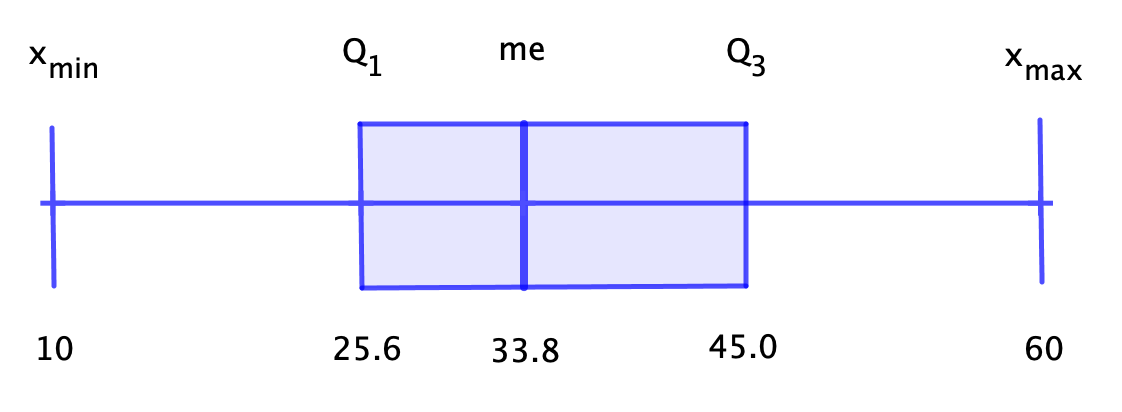
\includegraphics[width=.5\textwidth]{imagenes/imagenes01/T01IM39.png}
	\end{figure}

Se observa un cierto sesgo a la derecha.

\textcolor{blue}{------ $i)\ ]P_{40},P_{60}[$}

El valor central es la mediana, el $P_{50}$; el $20\%$ de los valores a su alrededor estarán comprendidos entre el $P_{40}$ y el $P_{60}$

$40\%(40)=20 \ \to \ P_{40}=30$

$60\%(40)=30 \ \to \ P_{60}=30+\dfrac{30-20}{13}\ 10=37.69$

El intervalo pedido es $\ [30,37.69]$

\vspace{5mm}%********************************
\begin{ejemplo}
\begin{ejer}
	Para los datos 7, 3, 4, 6, 4, 3, 3; calcula la media artimética, geométrica y armónica.
\end{ejer}	
\end{ejemplo}

\begin{table}[H]
\centering
\begin{tabular}{rrrrr}
\multicolumn{1}{c}{\textbf{$x_i$}} & \multicolumn{1}{c}{\textbf{$n_i$}} & \multicolumn{1}{c}{\textbf{$x_i\ n_i$}} & \multicolumn{1}{c}{\textbf{$x_i^{n_i}$}} & \multicolumn{1}{c}{\textbf{$n_1/x_i$}} \\ \hline
\multicolumn{1}{|r|}{3} & \multicolumn{1}{r|}{3} & \multicolumn{1}{r|}{9} & \multicolumn{1}{r|}{27} & \multicolumn{1}{r|}{1.00} \\ \hline
\multicolumn{1}{|r|}{4} & \multicolumn{1}{r|}{2} & \multicolumn{1}{r|}{8} & \multicolumn{1}{r|}{16} & \multicolumn{1}{r|}{0.50} \\ \hline
\multicolumn{1}{|r|}{6} & \multicolumn{1}{r|}{1} & \multicolumn{1}{r|}{6} & \multicolumn{1}{r|}{6} & \multicolumn{1}{r|}{0.17} \\ \hline
\multicolumn{1}{|r|}{7} & \multicolumn{1}{r|}{1} & \multicolumn{1}{r|}{7} & \multicolumn{1}{r|}{7} & \multicolumn{1}{r|}{0.14} \\ \hline
\multicolumn{1}{l|}{} & \multicolumn{1}{l|}{$N=8$} & \multicolumn{1}{l|}{$\Sigma \to 30$} & \multicolumn{1}{l|}{$\Pi \to 18144$} & \multicolumn{1}{l|}{$\sigma \to 1.81$} \\ \cline{2-5} 
\end{tabular}
\end{table}

$\bar x=\dfrac{\displaystyle \sum_{i=1}^4 x_i \cdot n_i}{N}=3.75; \quad$
$\bar x_g=\sqrt[8] {\displaystyle \prod_{i=1}^4 x_i^{n_i}}=3.41; \quad$
$\bar x_a=\dfrac{N}{\displaystyle \sum_{i=1}^4 \dfrac{n_i}{x_i} }=4.42$

\vspace{0.5mm} %**********************
\begin{destacado}
Diferencia entra variable discreta y continua a la hora del cálculo de parámetros de posición. 

En variable discreta para encontrar la posición del individuo adecuado usaremos una aproximación por defecto.	
\end{destacado}

\vspace{5mm}%********************************
\begin{ejemplo}
\begin{ejer}
	Para las dos siguientes distribuciones, encontrar el $P_{33}$
	
\begin{table}[H]
\centering
\begin{tabular}{r|r|rrrr|r|r}
\cline{1-3} \cline{5-8}
\multicolumn{3}{|c|}{\textbf{Distribución 1}} & \multicolumn{1}{c|}{\textbf{}} & \multicolumn{4}{c|}{\textbf{Distribución 2}} \\ \cline{1-3} \cline{5-8} 
\multicolumn{1}{|c|}{\textbf{$x_i$}} & \multicolumn{1}{c|}{\textbf{$n_i$}} & \multicolumn{1}{c|}{\textbf{$N_i$}} & \multicolumn{1}{c|}{\textbf{$\qquad$}} & \multicolumn{1}{c|}{\textbf{clase}} & \multicolumn{1}{c|}{\textbf{$x_i$}} & \multicolumn{1}{c|}{\textbf{$n_i$}} & \multicolumn{1}{c|}{\textbf{$N_i$}} \\ \cline{1-3} \cline{5-8} 
\multicolumn{1}{|r|}{3} & 3 & \multicolumn{1}{r|}{3} & \multicolumn{1}{r|}{} & \multicolumn{1}{r|}{[2,4[} & 3 & 3 & \multicolumn{1}{r|}{3} \\ \cline{1-3} \cline{5-8} 
\multicolumn{1}{|r|}{5} & 10 & \multicolumn{1}{r|}{10} & \multicolumn{1}{r|}{} & \multicolumn{1}{r|}{[4,6[} & 5 & 10 & \multicolumn{1}{r|}{10} \\ \cline{1-3} \cline{5-8} 
\multicolumn{1}{|r|}{7} & 15 & \multicolumn{1}{r|}{25} & \multicolumn{1}{r|}{} & \multicolumn{1}{r|}{[6,8[} & 7 & 15 & \multicolumn{1}{r|}{25} \\ \cline{1-3} \cline{5-8} 
\multicolumn{1}{|r|}{9} & 7 & \multicolumn{1}{r|}{35} & \multicolumn{1}{r|}{} & \multicolumn{1}{r|}{[8,10[} & 9 & 7 & \multicolumn{1}{r|}{35} \\ \cline{1-3} \cline{5-8} 
\multicolumn{1}{c|}{} & \multicolumn{1}{c|}{N=35} & \multicolumn{1}{c}{} & \multicolumn{1}{c}{} & \multicolumn{1}{c}{} & \multicolumn{1}{c|}{} & \multicolumn{1}{c|}{N=25} & \multicolumn{1}{c}{} \\ \cline{2-2} \cline{7-7}
\end{tabular}
\end{table}
\end{ejer}	
\end{ejemplo}

Para la distribución 1: $\ 33\%(35)=11.55 \to 12^o$ individuo deja tras de sí al (más) 33\% de los individuos de la población.

El valor de la variable para este $12^o$ individuo es $ \ P_33=7$

Para la distribución 2: $\ 33\%(35)=11.55 \to P_{33}=6+\dfrac{11.55-10}{15}\ 2=6.21$

\vspace{5mm}%********************************
\begin{ejemplo}
\begin{ejer}
	Una varable estadística $X$ tiene una media $\bar x=20$ y una desviación típica $s_x=5$. Si elevamos al cuadrado todos los datos, ?`cuál será ahora el valor de la media?
\end{ejer}	
\end{ejemplo}

$x_i \to y_i=x_i^2 \ \Rightarrow \  s_x^2=\dfrac{\displaystyle \sum n_i\cdot x_i^2}{N}- {\bar x}^2=\bar y-{\bar x}^2$

$\bar y={\bar x}^2+s^2x \ \to \ \bar y=20^2+5^2=425$


\vspace{5mm}%********************************
\begin{ejemplo}
\begin{ejer}
	Una variable estadística tiene $\bar x=8$ y $s_x=2$. ?`Qué transformación hay que hacer a la variable para que su nueva media sea $\bar y=42$ y la nueva desviación típica $s_y=10$
\end{ejer}	
\end{ejemplo}

El cambio lineal general es: $y_i=a+bx_i \ \vee \ Y=a+bX$
 
$\begin{cases}
\bar y &= a + bx \\
s_y &= bs_x	
\end{cases}
\to 
\begin{cases}
42&=a+8b\\ 10&=2b	
\end{cases} \to b=5;\  a=2 \ \Rightarrow \ Y=2+5X \ \ \ \textcolor{gris}{or\ y_i=2+5x_i}$


\vspace{5mm} %************************
\begin{ejemplo}
\begin{ejer}
Calcula la tasa covid 14 días para todo el territorio español $\to$ \textsf{``media ponderada''}.
	

	\begin{figure}[H]
			\centering
			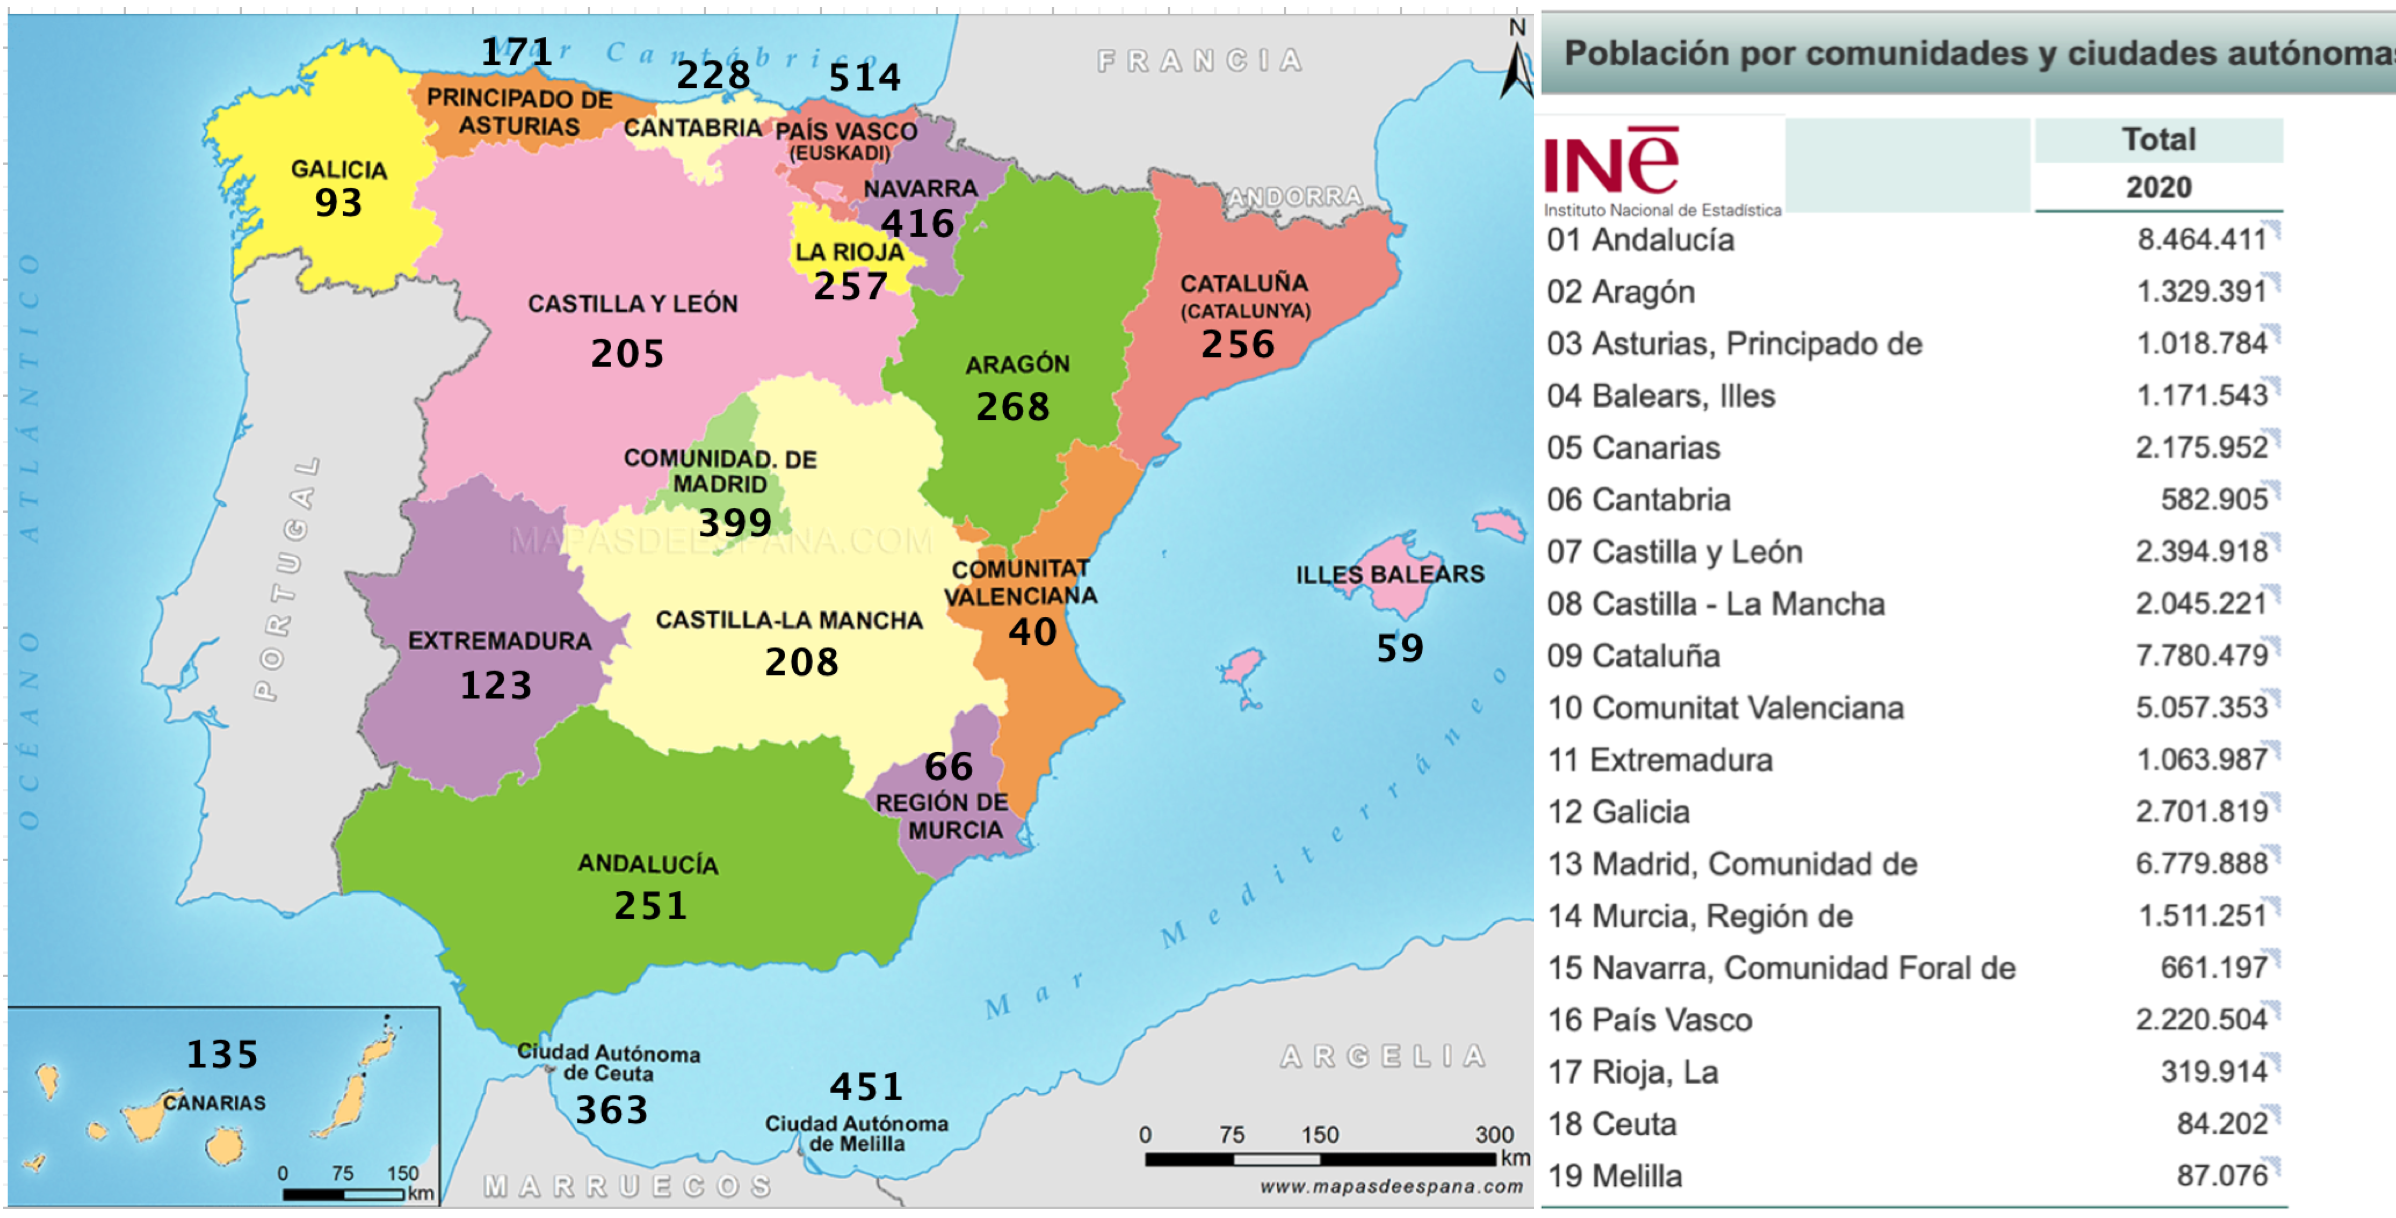
\includegraphics[width=1\textwidth]{imagenes/imagenes01/T01IM40.png}
	\end{figure}
\end{ejer}	
\end{ejemplo}

En el mapa (cartograma) aparece la incidencia acumulada de contagios en 14-días por cada 100.000 habitantes, a la derecha se muestra la población de cada comunidad autónoma.

Tomaremos como variable $x_i$ la incidencia acumulada por 100K habitantes de cada una de las 19 comunidades y ciudades autónomas de España y como frecuencia absoluta de cada una, $n_i$, la población. Así,

$\bar x_p=\displaystyle \sum_{i=1}^{19} x_i \cdot n_i \ / \  \sum_{i=1}^{19} n_i = 232.2$

\begin{destacado}
\emph{Todo lo visto en este tema se puede hacer, más rápidamente, con el múltiple sw existente, pero se ha optado por presentar todos los cálculos a mano por motivos didácticos.}
\end{destacado}




\section{Curiosidades}

\begin{myexampleblock}{Cómo mentir con estadísticas}

\emph{``Hay tres tipos de mentiras: mentiras, malditas mentiras y estadísticas’’}\footnote{Basado en el artículo de Francisco J. Lastra}; popularizada en los Estados Unidos por Mark Twain, esta frase describe el abuso de estadísticas para reforzar argumentos falaces.

\vspace{2mm} Un buen gráfico permite sintetizar información numérica, es difícil no convencerse de cualquier cosa cuando se acompaña la idea con gráficos. 

\vspace{2mm} La misma información se puede utilizar para crear dos gráficos con mensajes totalmente opuestos. Detrás de una estadística hay, sin duda, mucho más allá que figuras representativas de números, y es debido a esto que hoy existen expertos en el ``entendimiento de riesgo’’, estadísticos que trabajan con matemáticos, psicólogos y otros profesionales para transmitir al público de forma precisa sus hallazgos.

\vspace{2mm} ``Los gráficos pueden ser tan manipuladores como las palabras’’, por eso, ser capaces de leer, entender y evaluar estadísticas es una habilidad fundamental y estar atentos a los trucos que pueden hacernos caer en un error o engaño es una necesidad.

\vspace{2mm} Algunos casos de mentiras estadísticas, que rescatan los matemáticos Andrew Gelman y Deborah Nolan en su libro Teaching Statistics: A Bag of Tricks, son:

\vspace{2mm} \textbf{1. Inventar cifras}

\vspace{2mm} Según un estudio de la Universidad de Cambridge, un 53,4\% de las estadísticas son inventadas. Suena inteligente,¿`no?. Inventar estadísticas es la forma más directa de engaño de la que hablaremos y es, lamentablemente, más común de lo que se pensaría, gracias al aura de verdad o seriedad que un porcentaje o un grupo de barras puede darle al mensaje que lo acompaña.

\vspace{2mm} Uno de los ejemplos más recientes y notables por su impacto, y que afortunadamente fue desbaratado con rapidez, fue un tuit publicado por el candidato republicano Donald Trump.

\vspace{2mm} En diciembre del año pasado, Trump retuiteó estadísticas que señalaban, entre otras cosas, que un 81\% de los asesinatos de gente blanca era cometidos por gente negra.

\begin{multicols}{2}
	\begin{figure}[H]
			\centering
			
\includegraphics[width=.5\textwidth]{imagenes/imagenes01/T01IM30.png}
	\end{figure}
	
	\begin{figure}[H]
			\centering
			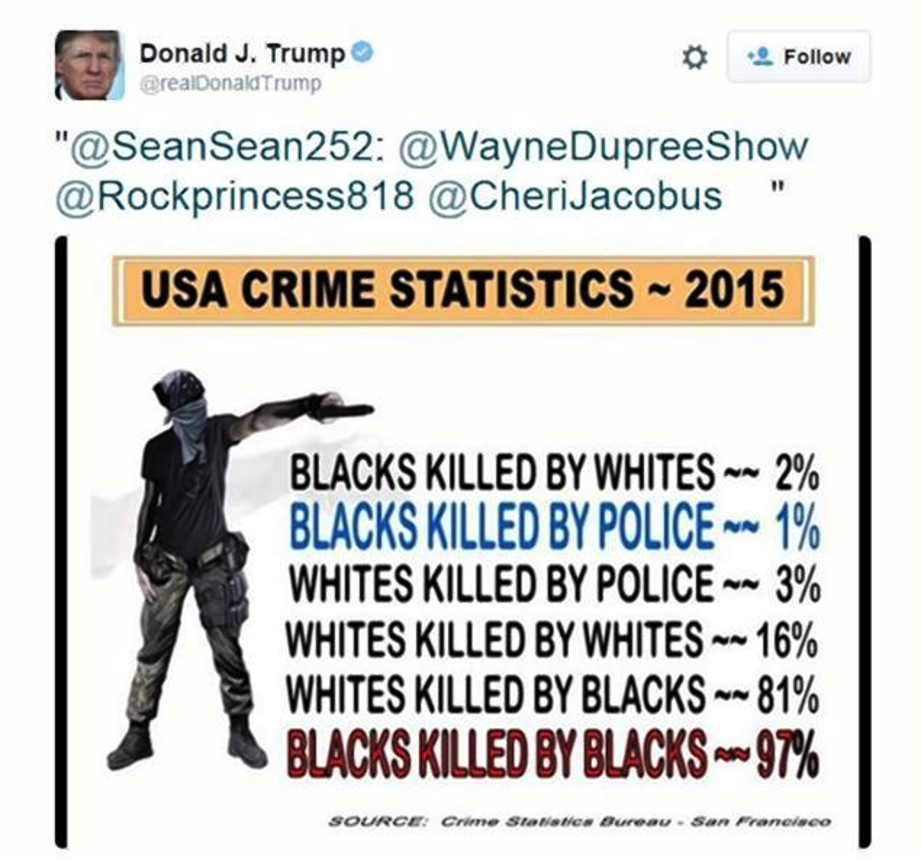
\includegraphics[width=.5\textwidth]{imagenes/imagenes01/T01IM31.png}
	\end{figure}
\end{multicols}


\vspace{2mm} Una rápida consulta de las cifras oficiales del FBI arrojó que el porcentaje, en realidad, asciende a un 15\% y que la supuesta fuente, la Oficina de Estadísticas Criminales de San Francisco, jamás ha existido.

\vspace{2mm} Si bien Twitter, y en especial Trump, no dejan la vara muy alta en cuanto a veracidad de información se trata, no deja de ser impactante el peso que una estadística totalmente inventada de una oficina que jamás existió pudo tener en un mensaje.

\vspace{2mm} La lección es clara y se aplica a todo tipo de información sensible: \emph{hay que revisar la fuente de cualquier estadística que nos presenten}.

\vspace{2mm} \textbf{2. Cortar ejes}

\vspace{2mm} En el colegio nos enseñan que los ejes, tanto el ``X'' (horizontal) como el ``Y'' (vertical), parte de 0, pero esto no siempre ocurre en los gráficos. No es algo prohibido ni malo necesariamente, pero se presta para exagerar o minimizar deliberadamente comparaciones de cifras.

\vspace{2mm} Existen muchas formas de alterar ejes, pero la más común es la que se aprecia en las siguientes imágenes. Nótese que se trata de exactamente los mismos datos, solo que en el primero buena parte del eje Y (el vertical) fue truncado para hacer, suponemos, leña (;-). Así, la diferencia entre cada barra se ve enorme, cuando al verla en el contexto total (segundo gráfico), la diferencia es mínima.

\begin{multicols}{2}
	\begin{figure}[H]
			\centering
			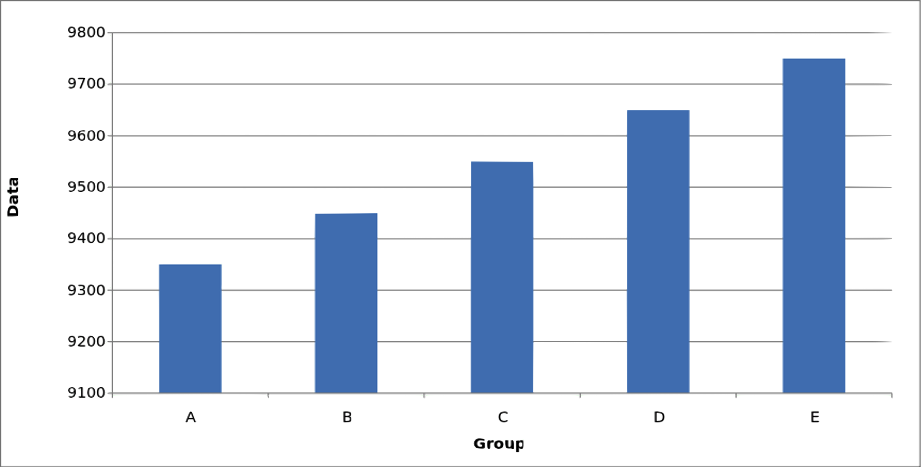
\includegraphics[width=.5\textwidth]{imagenes/imagenes01/T01IM32.png}
	\end{figure}
	
	\begin{figure}[H]
			\centering
			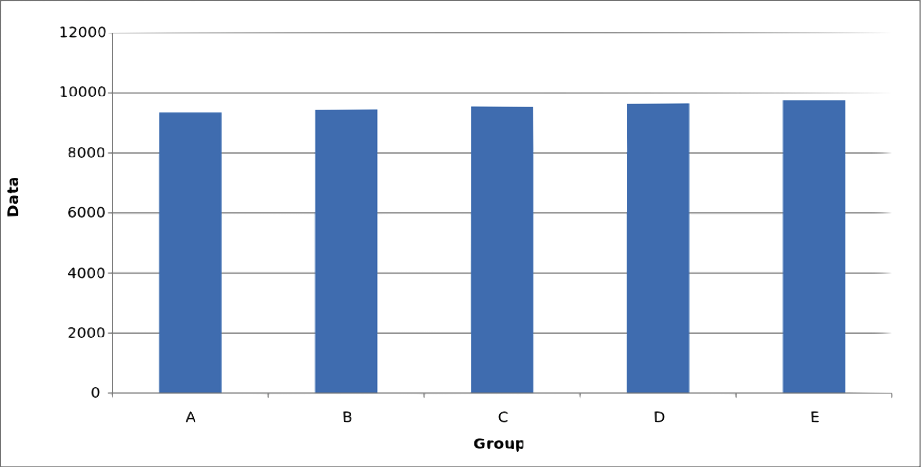
\includegraphics[width=.5\textwidth]{imagenes/imagenes01/T01IM33.png}
	\end{figure}
\end{multicols}


\begin{multicols}{2}
	\begin{figure}[H]
			\centering
			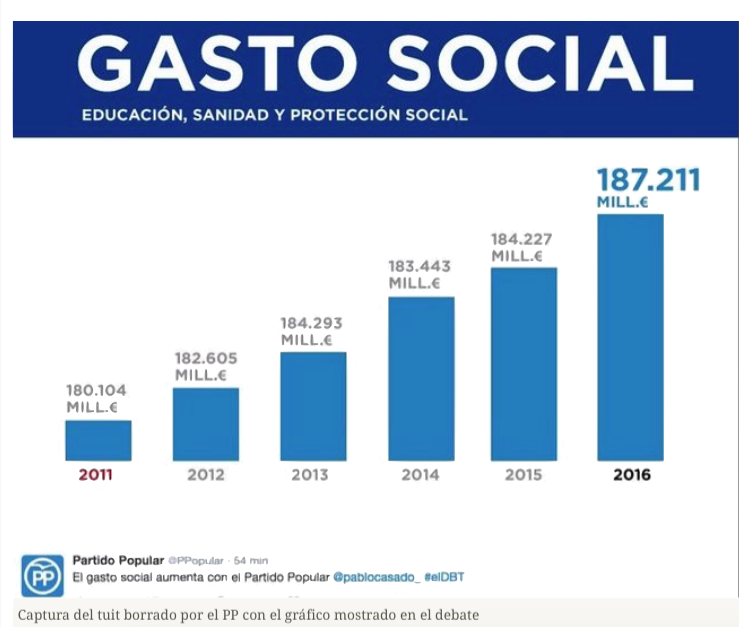
\includegraphics[width=.5\textwidth]{imagenes/imagenes01/T01IM34.png}
	\end{figure}
	
	\textcolor{white}{.}
	
	\begin{figure}[H]
			\centering
			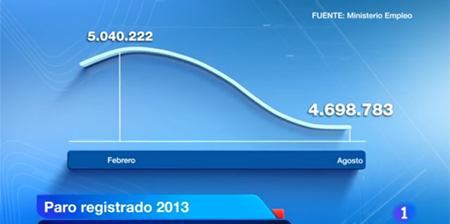
\includegraphics[width=.5\textwidth]{imagenes/imagenes01/T01IM35.png}
	\end{figure}
\end{multicols}



\vspace{2mm} Lo mismo ocurre con las secuencias de tiempo (habitualmente situadas en el eje X). El crecimiento o disminución de la delincuencia, economía, desempleo, IPC, etc. puede verse impresionante o irrelevante según qué período se tome. Habitualmente los políticos seleccionan los marcos de tiempo que mejor hacen ver su gestión.

\vspace{2mm} La próxima vez que veas uno de estos gráficos \emph{!`Asegúrate que partan de 0! O al menos, que consideren un marco de referencia suficientemente amplio para tener claro cuán relevante es la estadística}.

\vspace{2mm}  \textbf{3. Otras representaciones erróneas}

\vspace{2mm}  En el siguiente gráfico, a igualdad de frecuencia relativa para los sectores rojo y morado, el efecto 3D hace que al aparecer el sector morado más próximo al observador aumente su proporción respecto al sector rojo. También aumenta el efecto aparente de tamaño el hecho de extraer un sector de la tarta (el verde).

\begin{figure}[H]
			\centering
			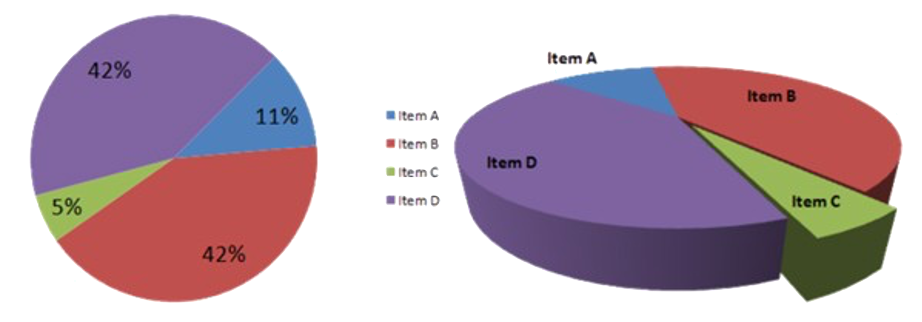
\includegraphics[width=.9\textwidth]{imagenes/imagenes01/T01IM38.png}
	\end{figure}

\vspace{2mm}  Uno de los más frecuentes errores de diseño en gráficos, y que ocurre hasta en los diarios y revistas más prestigioso, es usar dibujos con área o volumen, para representar un dato que debería tener un solo eje. Aunque se hace con un objetivo decorativo, el lector no sabe si debe comparar sólo la altura, el área o el volumen del objeto.

\begin{multicols}{2}
	\begin{figure}[H]
			\centering
			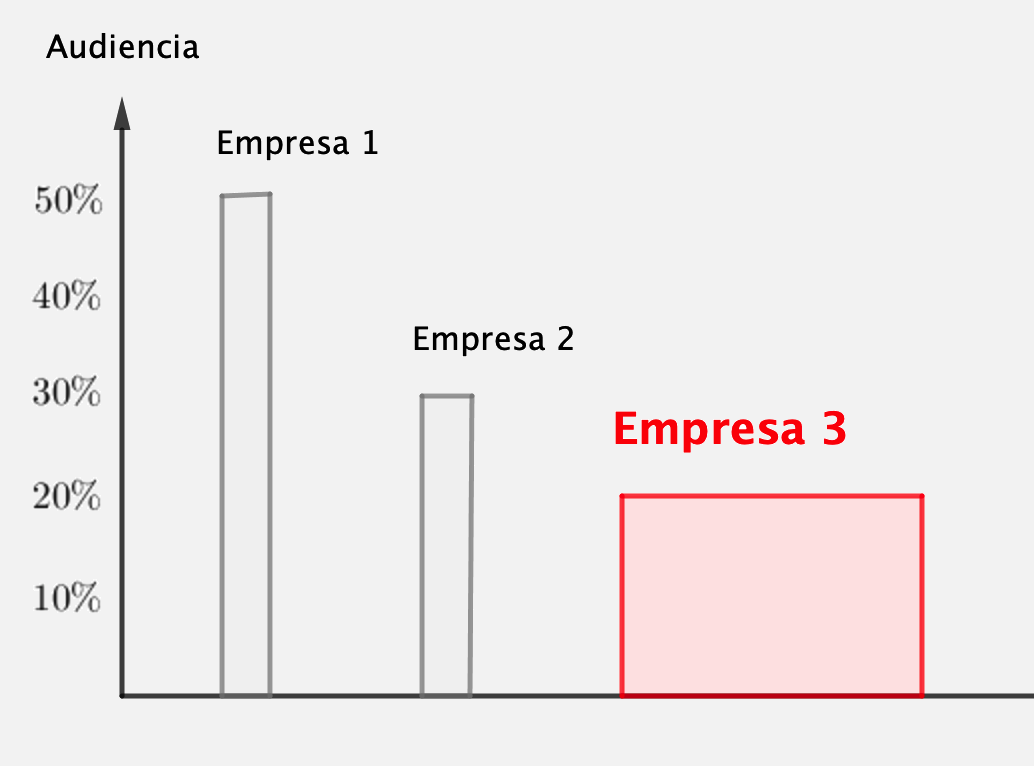
\includegraphics[width=.5\textwidth]{imagenes/imagenes01/T01IM36.png}
	\end{figure}
	
	\begin{figure}[H]
			\centering
			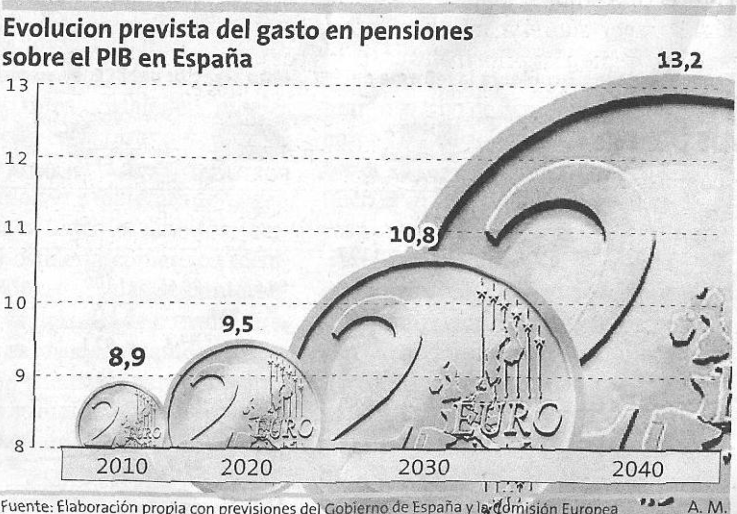
\includegraphics[width=.5\textwidth]{imagenes/imagenes01/T01IM37.png}
	\end{figure}
\end{multicols}


\vspace{2mm}  Aunque parezcan muchas cosas de las que estar preocupado, en realidad se trata de tener la misma actitud que frente a un estudio: \emph{ser escéptico}. En otras palabras, verificar que la fuente sea fiable (y que exista), que sus elementos tengan las proporciones correctas, y que la información que transmite (los números) sea la misma que nos dicen que transmite con los gráficos que la acompañan.


\end{myexampleblock}


\newpage

$\quad$

$\quad$



\begin{myblock}{RESUMEN Estadística descriptiva unidimensional}

$ \quad $

\begin{table}[H]
\centering
\begin{tabular}{c|c|c|c|c|c|c}
\hline
\multicolumn{1}{|c|}{$x_i$} & $n_i$ & $f_i$ & $N_i$ & $F_i$ & $x_i \cdot n_i$ & \multicolumn{1}{c|}{$x_i^2 \cdot n_i$} \\ \hline
\multicolumn{1}{|c|}{$\vdots$} & $\vdots$ & $\vdots$ & $\vdots$ & $\vdots$ & $\vdots$ & \multicolumn{1}{c|}{$\vdots$} \\ \hline
 & N & 1 &  &  & $\sum \to \bar x$ & $\sum \to s$
 
\end{tabular}
\end{table}
	
 $\triangleright \ $ Media(s):
  
 $$ \boxed{\ \bar x=\dfrac{\displaystyle \sum_{i=1}^n \ x_i \cdot n_i}{N} \ }
 \qquad  \quad
 \bar x_p=\dfrac{\sum x_i \cdot p_i}{\sum p_i} 
 \qquad \quad
 \bar x_g=\sqrt[N]{\prod x_i ^{n_i} } 
 \qquad \quad
 \bar x_a= \dfrac{N}{\sum \frac{x_i}{x_i}}$$
 
 \vspace{5mm} $\triangleright \ $ Moda:
 
 $$ mo\ = \ L_k + \dfrac{n_k-n_{k-1}}{(n_k-n_{k-1})+(n_k-n_{k+1})} \cdot c_k$$
 
 \vspace{5mm}  $\triangleright \ $ Mediana, Cuartiles, Deciles y Percentiles:
 
 $$me \ = \ L_k+\dfrac{ \frac N 2 + N_{k-1}}{n_k}\cdot c_k\ ; 
 \qquad  \qquad \qquad \qquad
 Q_i \ = \ L_k+\dfrac{i\cdot \frac N 4 + N_{k-1}}{n_k}\cdot c_k ;	\ \ i=1,2,3$$
 
 $$D_i \ = \ L_k+\dfrac{i\cdot \frac N {10} + N_{k-1}}{n_k}\cdot c_k ;	\ \ i=1,2,\cdots , 9 ; \qquad 
 P_i \ = \ L_k+\dfrac{i\cdot \frac N {100} + N_{k-1}}{n_k}\cdot c_k ;	\ \ i=1,2,\cdots , 99 $$
  
\vspace{5mm}  $\triangleright \ $ Varianza y desviación típica: 

$$ s^2 \ = \ \dfrac{\displaystyle \sum_{i=1}^n\ (x_i-\bar x)^2\cdot n_i}{N} \ = \ \dfrac{\sum x_i^2\cdot n_i}{N} - \bar x^2
\qquad \qquad \qquad \qquad 
s \ = \ \sqrt{s^2} $$

\vspace{5mm}  $\triangleright \ $ Coeficiente de variación (Pearson) y tipificación: 

$$ CV \ = \ \dfrac {s}{\bar x}
\qquad \qquad  
z_i \ = \ \dfrac {x_i-\bar x}{s}$$

$ \quad $

\end{myblock}

	
\chapter{Distribuciones bidimensionales: Correlación y Regresión lineal}
\chaptermark{Estad. 2-D: Correlación y Regresión}

%*************************************************************************
% ATENcION: por cambio ordenación temas, 2 <--> 3, las imagenes de 3.Prob. 
%están en imagenes02 y las imágenes de 2.Estad 2D están en imagenes03.
%*************************************************************************

\begin{tikzpicture}
	\fill [left color=red!50, right color=teal!50] (0,0) rectangle (6.5,.1);
	\fill [left color=teal!50, right color=green!50] (6.5,0) rectangle (11.5,.1);
	\end{tikzpicture}




\section[Distribuciones estadísticas bidimensionales]{Distribuciones estadísticas bidimensionales \sectionmark{Distribuciones 2-Dim}}
 \sectionmark{Distribuciones 2-Dim}



\begin{definition}


	

\begin{multicols}{2}
 
Si de una determinada muestra o población se estudian dos caracteres simultneamente, se obtienen dos series de datos de la forma:
 
\begin{table}[H]
\centering
\begin{tabular}{c|cccccc}
\textbf{$x_i$} & $x_1$ & $x_2$ & $x_3$ & $\cdots$ & $\cdots$ &  \\ \cline{1-6}
\textbf{$y_i$} & $y_1$ & $y_2$ & $y_3$ & $\cdots$ & $\cdots$ &  \\ \cline{1-6}
\textbf{$n_i$} & $n_1$ & $n_2$ & $n_3$ & $\cdots$ & $\cdots$ & $\ \to \Sigma N$
\end{tabular}
\end{table}
 
\end{multicols} 


 
Donde $x_i$ e $y_i$ son las variables estadísticas correspondientes a las carateristicas observadas y $n_i$ es la frecuencia absoluta de cada pareja de datos $(x_i,y_i)$, es decir, $n_i$ es el número de veces que se repite el par $(x_i,y_i)$.
 
\vspace{2mm}  A la lista de estos pares ordenados de datos con sus respectivas frecuencias se le llama \textbf{\emph{variable estadística bidimensional}}, $\ \boldsymbol{ (x_i, \ y_i; \ n_i)}$.

\vspace{2mm} La frecuencia relativa del par $(x_i,y_j)$ es $f_{i j} = n_{i j}/N$ , donde $N$ denota el número total de pares observados.

\vspace{2mm} Las \textbf{\emph{variables marginales}}\footnote{Las distribuciones marginales son las distribuciones unidimensionales que nos informan del número de observaciones para cada valor de una de las variables, prescindiendo de la información sobre los valores de las demás variables.} $X$ e $Y$ toman los valores $\{x1,x2,...,xm\},$  $\{y1,y2,...,yr\}$ para ciertos $m$, $r$, respectivamente, y la variable bidimensional $(X,Y)$ tomará los valores $\{(xi,yj)\}\ 1\le i \le m,\ 1 \le j \le r$.
 
\end{definition}
 

\begin{example}

Se muestran algunos ejemplos de variables bidimensionales:

\begin{itemize}

\item $(X,Y)$ (sexo, color del ojos); $X$ cualitativa; $Y$ cualitativa.

\item $(X,Y)$ (nivel de estudios, lustros en la empresa); $X$ cualitativa; $Y$ cuantitativa (discreto -años-).

\item $(X,Y)$ (número de hermanos, número de hijos); $X$ cuantitativa (v.e. discreta); $Y$ cuantitativa (v.e. discreta).

\item $(X,Y)$ (peso, estatura); $X$ cuantitativa (v.e. continua); $Y$ cuantitativa (v.e. continua).

En este tema nos interesarán las variables estadísticas bidimensionales en que ambas sean cuantitativas.
\end{itemize}
\end{example}

\begin{theorem}
.	Nótese que:

$$\displaystyle \sum_{i=1}^m \ \sum_{j=1}^r\ n_{ij}\ = \ N;\qquad 	\qquad \qquad\sum_{i=1}^m \ \sum_{j=1}^r\ f_{ij}\ = \ 1$$
\end{theorem}



\subsection{Distribuciones de frecuencias}
	


\begin{definition}
.	Se define la \textbf{frecuencia (absoluta) marginal} del valor $x_i$ como la suma de las frecuencias correspondientes a los pares $(x_i,y_j)$, para $1 \le  j \le  r$:
	

Análogamente se define la frecuencia (absoluta) marginal del valor $y_j$:

$$n_{x_i}=\displaystyle \sum_{j=1}^r\ n_{ij}; \qquad \qquad \qquad n_{y_j}=\displaystyle \sum_{i=1}^m\ n_{ij}$$
\end{definition}



\begin{theorem}
.	Nótese que $n_{x_i}$ (respectivamente, $n_{y_j}$ ) representa el número de veces que aparece el valor $x_i$ (respectivamente, $y_j$) en el total de pares obtenidos. Se verifica:

$$\displaystyle \sum_{i=1}^m\ n_{x_i}=\sum_{i=1}^m\ \sum_{j=1}^r\ n_{ij}=N; \qquad \qquad \qquad
\sum_{j=1}^r\ n_{x_i}=\sum_{j=1}^r\ \sum_{i=1}^m\ n_{ij} = N$$	
\end{theorem}



	



A partir de las frecuencias absolutas marginales se obtienen las frecuencias relativas marginales.

\begin{definition}
.	 Se definen las \emph{frecuencias relativas marginales} como:

$$\displaystyle f_{x_i}= \dfrac{n_{x_i}}{N};\qquad \qquad \qquad 
f_{y_j}= \dfrac{n_{y_j}}{N}$$	
\end{definition}

\vspace{5mm} %********************************
\begin{theorem}
.	Las frecuencias relativas marginales cumplen:

$$\displaystyle \sum_{i=1}^n\ f_{x_i} \ = \ \dfrac 1 N \ \sum_{i=1}^m\ n_{x_i}=1
\qquad \qquad \qquad   
\sum_{i=1}^n\ f_{y_j} \ = \ \dfrac 1 N \ \sum_{j=1}^r\ n_{y_j}=1$$	
\end{theorem}

\vspace{5mm} %********************************
Todos estos datos se pueden representar en una \colorbox{orange!10}{\textbf{\emph{``tabla de doble entrada''}}} \textcolor{gris}{(así se entenderá mejor)}:


	
\begin{table}[H]
\large
\centering
\begin{tabular}{c|c|c|c|c|c|c}
\cline{1-5}
\multicolumn{1}{|c|}{\textbf{$\ Y \  /  \ X$}} & \textbf{$\boldsymbol{y_1}$} & \textbf{$\boldsymbol{y_2}$} & \textbf{$\cdots$} & \textbf{$\boldsymbol{y_r}$} & \scriptsize{marg X} & \scriptsize{rel X} \\ \hline
\multicolumn{1}{|c|}{\textbf{$\boldsymbol{x_1}$}} & $n_{11}$ & $n_{12}$ & $\cdots$ & $n_{1r}$ & $n_{x_1}$ & $f_{x_1}$ \\ \hline
\multicolumn{1}{|c|}{\textbf{$\boldsymbol{x_2}$}} & $n_{21}$ & $n_{22}$ & $\cdots$ & $n_{2r}$ & $n_{x_2}$ & $f_{x_2}$ \\ \hline
\multicolumn{1}{|c|}{\textbf{$\cdots$}} & $\cdots$ & $\cdots$ & $\cdots$ & $\cdots$ & $\cdots$ & $\cdots$ \\ \hline
\multicolumn{1}{|c|}{\textbf{$\boldsymbol{x_m}$}} & $n_{m1}$ & $n_{m2}$ & $\cdots$ & $n_{mr}$ & $n_{x_m}$ & $f_{x_m}$ \\ \hline
\multicolumn{1}{c|}{\scriptsize{marg Y}} & $n_{y_1}$ & $n_{y_2}$ & $\cdots$ & $n_{y_r}$ & \textbf{$\boldsymbol{N}$} &  \\ \cline{1-5}
\scriptsize{rel. Y} & $f_{y_1}$ & $f_{y_2}$ & $\cdots$ & $f_{y_r}$ &  & \textbf{$\boldsymbol{1}$}
\end{tabular}
\end{table}

En la práctica, alguna de las $n_{ij}$ puede ser cero (la podemos dejar en blanco).


\vspace{10mm} %********************************
\begin{example}
. Construir una tabla simple y una de doble entrada para los siguientes datos de alturas, $x_i \ (\mathrm m)\ $  y pesos $y_i \ (\mathrm m)$.

\vspace{3mm} (1.55,65), (1.62,71), (1.73,75), (1.77,72), (1.72,81), (1.58,79), (1.68,72), (1.85,85), (1.77,77), (1.85,83), (1.67,81), (1.68,78), (1.79,78), (1.62,69)

\vspace{3mm} Agrupamos los datos en intervalos: $X \to [150,160[,\ [160,170[,\ [170,180[$ e $Y\to [60,70[, \ [70,80[,\ [80,90[$. Vamos poniendo cada dato en la casilla correspondiente. (Puede ponerse la X/Y en vertical u horizontal en la tabla de doble entrada, como se desee). Para cálculos posteriores se trabajará con las \emph{marcas de clase.}

\begin{table}[H]
\centering
\begin{tabular}{c|c|c|c|c}
$\boldsymbol{\downarrow X \ \ / \ \ Y \rightarrow}$ & \textbf{{[}60,70{[}$\to 65$} & \textbf{{[}70,80{[}$\to 75$} & \textbf{{[}80,90{[}$\to 85$} & \textbf{$n_{x_i}$} \\ \hline
\textbf{{[}150,160{[}$\to 155$} & 1 & 1 & 0 & 2 \\ \hline
\textbf{{[}160,170{[}$\to 165$} & 1 & 3 & 1 & 5 \\ \hline
\textbf{{[}170,180{[}$\to 175$} & 0 & 4 & 1 & 5 \\ \hline
\textbf{{[}180,190{[}$\to 185$} & 0 & 0 & 2 & 2 \\ \hline
\textbf{$n_{y_j}$} & 2 & 8 & 4 & \textbf{14}
\end{tabular}
\end{table}

Para la tabla de simple entrada, o bien leyendo los datos originales, o bien los de la tabla de doble entrada, los escribimos ahora en horizontal y con las variables representadas por sus marcas de clase (leemos por filas en la tabla de doble entrada).

\begin{table}[H]
\centering
\begin{tabular}{c|ccccccccc}
$\boldsymbol{x_i}$ & 155 & 155 & 165 & 165 & 165 & 175 & 175 & 185 &  \\ \cline{1-9}
$\boldsymbol{y_i}$ & 65 & 75 & 65 & 75 & 85 & 75 & 85 & 85 &  \\ \cline{1-9}
$\boldsymbol{n_i}$ & 1 & 1 & 1 & 3 & 1 & 4 & 1 & 2 & $\quad \to \boldsymbol{14}$
\end{tabular}
\end{table}
	
	Para trabajar numéricamente con la tabla es mejor la forma sencilla que la de doble entrada.
\end{example}

%\vspace{5mm}

En las tablas de doble entrada, cuando algún valor de los $n_{ij}$ es cero, puede dejarse la celda en blanco.

\begin{table}[H]
\centering
\begin{tabular}{c|c|c|c|c}
$\boldsymbol{\downarrow X \ \ / \ \ Y \rightarrow}$ & \textbf{{[}60,70{[}$\to 65$} & \textbf{{[}70,80{[}$\to 75$} & \textbf{{[}80,90{[}$\to 85$} & \textbf{$n_{x_i}$} \\ \hline
\textbf{{[}150,160{[}$\to 155$} & 1 & 1 &   & 2 \\ \hline
\textbf{{[}160,170{[}$\to 165$} & 1 & 3 & 1 & 5 \\ \hline
\textbf{{[}170,180{[}$\to 175$} &   & 4 & 1 & 5 \\ \hline
\textbf{{[}180,190{[}$\to 185$} &   &   & 2 & 2 \\ \hline
\textbf{$n_{y_j}$} & 2 & 8 & 4 & \textbf{14}
\end{tabular}
\end{table}


\subsection{Representación gráfica de variables bidimensionales}

\begin{definition}
.	Si en la variable estadística bidimensional 	todas las frecuencias absolutas de los pares de valores son 1, basta con representar los pares de valores en un diagrama X-Y. Es el llamado \textbf{diagrama de dispersión} o \textbf{nube de puntos}.

\vspace{2mm} Siguiendo con la distribición del ejemplo anterior, 

	\begin{figure}[H]
			\centering
			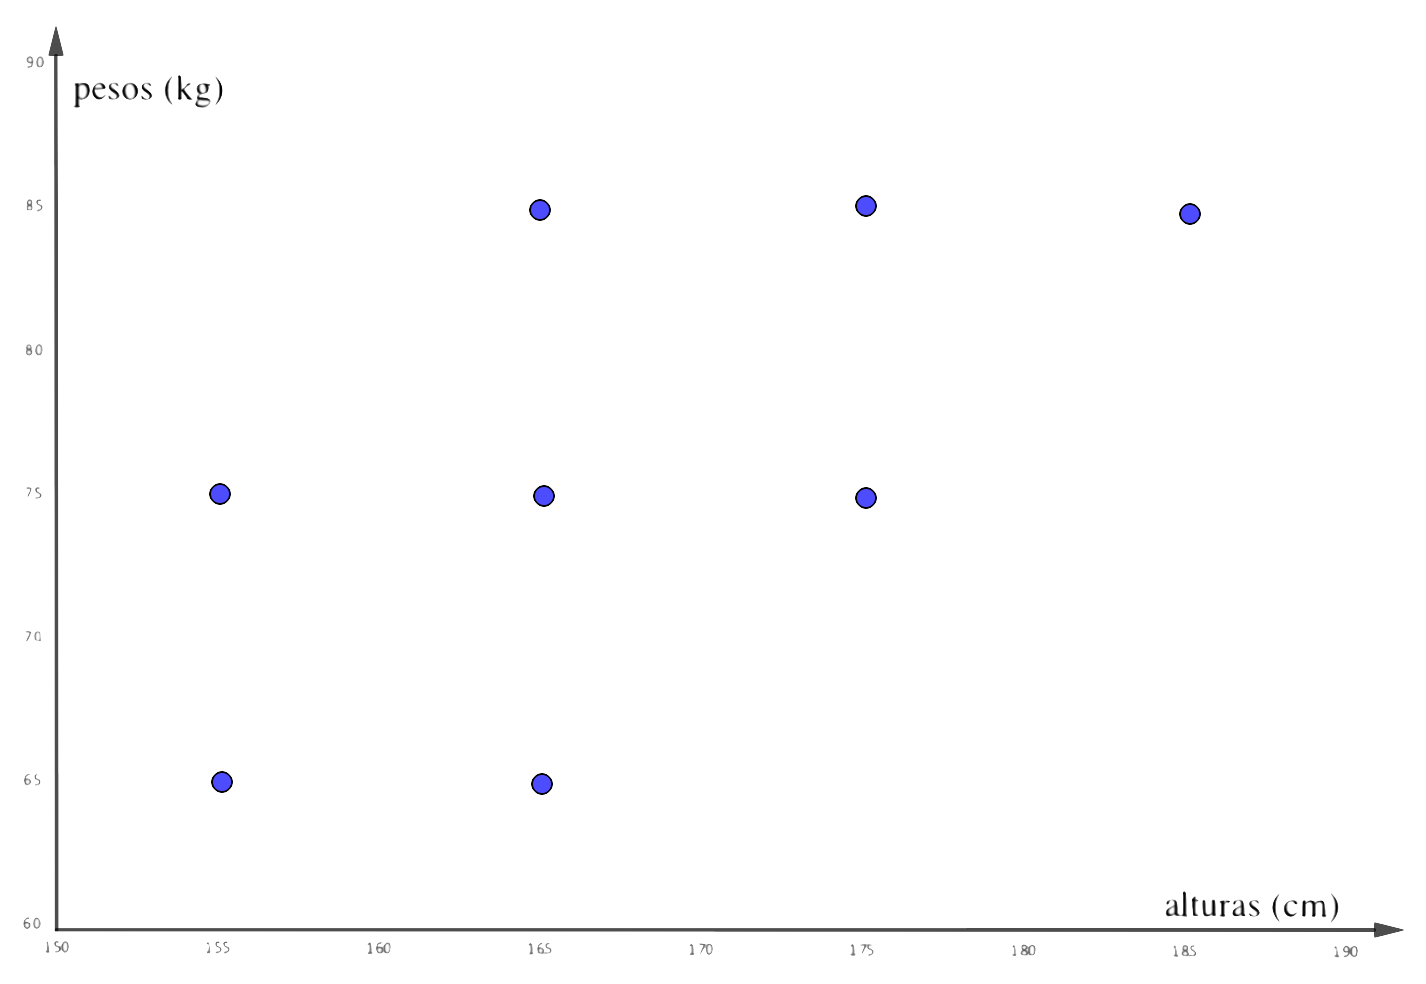
\includegraphics[width=0.75\textwidth]{imagenes/imagenes03/T03IM01.png}
	\end{figure}

Si cada par de variables tiene su propia frecuencia tenemos dos soluciones: o bien dibujamos tantos puntos próximos entre sí como indique la frecuencia absoluta, o bien dibujamos para cada pareja de valores círculos de área proporcional a la frecuencia absoluta de los mismos ($A=\pi r^2 \propto n_{ij} \to r \propto \sqrt{n_{ij}};\ $ --- \textcolor{gris}{$\propto$ es el símbolo de proporcionalidad}).

\begin{figure}[H]
			\centering
			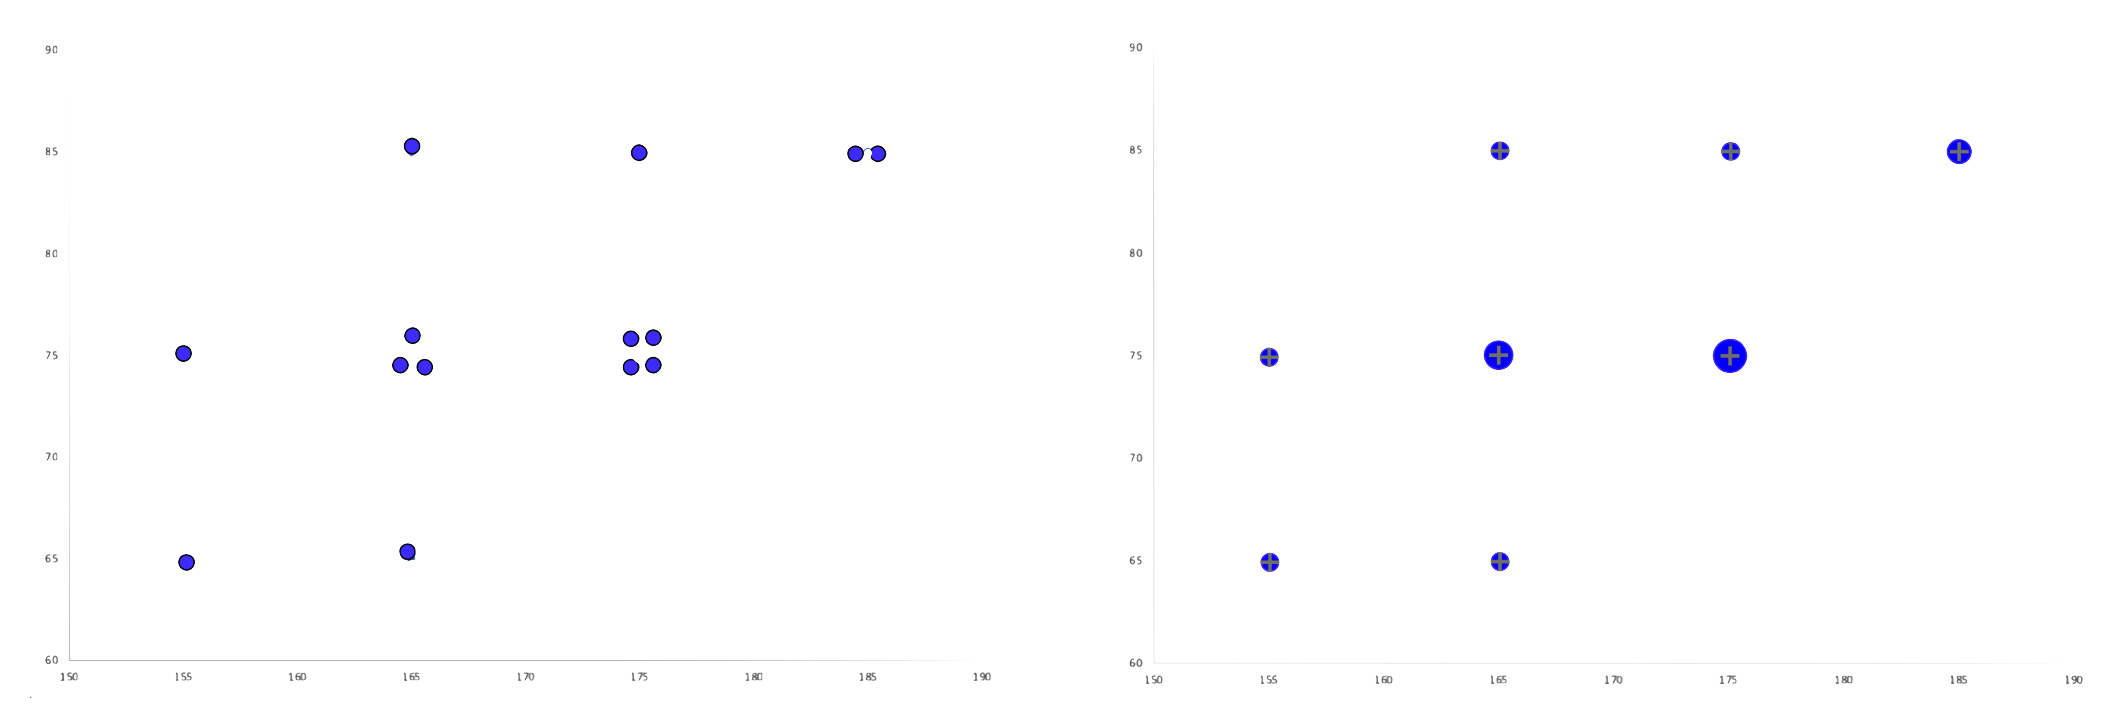
\includegraphics[width=0.95\textwidth]{imagenes/imagenes03/T03IM02.png}
	\end{figure}

Otra posibilidad es usar el \emph{prismograma}, es una representación 3D, en la base se representa la variable X-Y, $(x_i,y_i)$, y como altura la frecuencia absoluta de cada valor de la variable bidimensional, $n_{ij}$, formando una barra o un prisma (todos de la misma base).

	\begin{figure}[H]
			\centering
			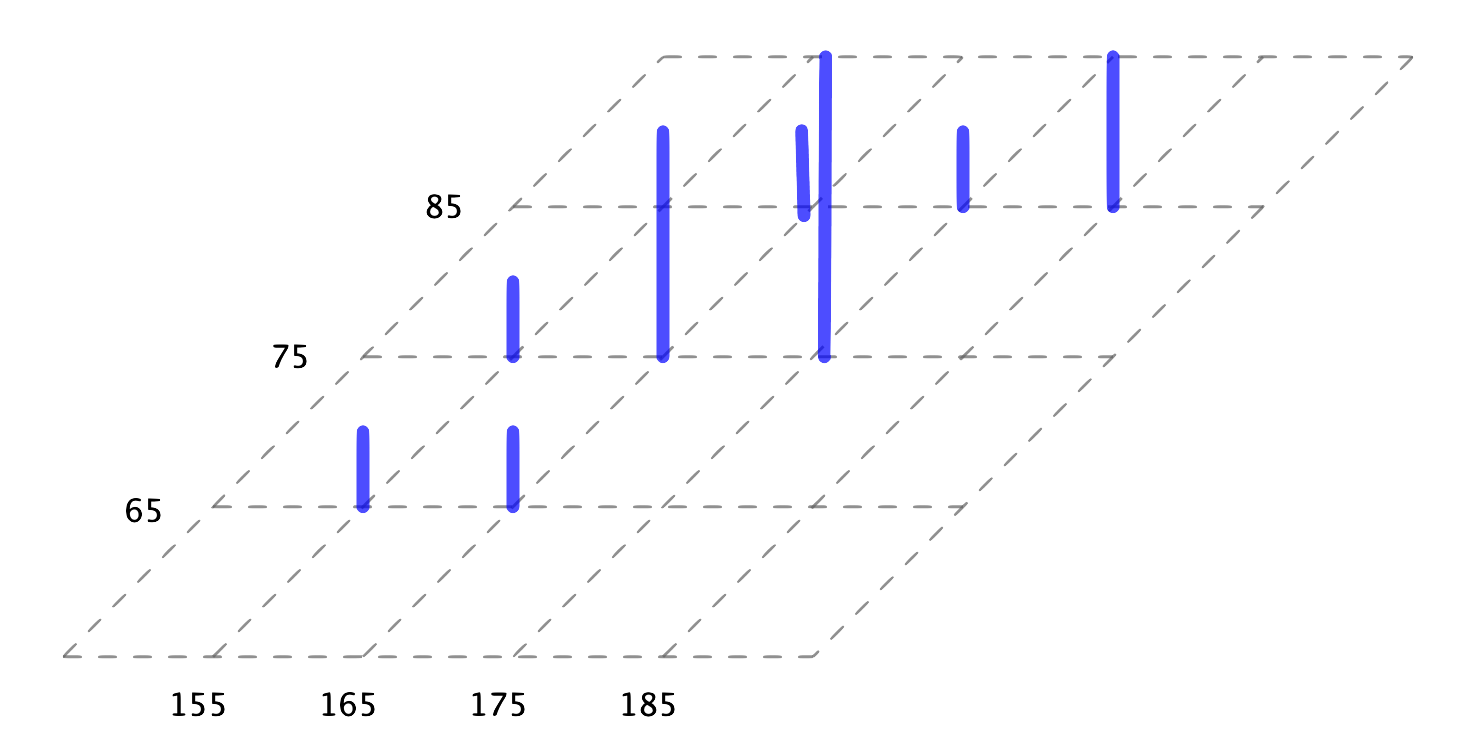
\includegraphics[width=0.65\textwidth]{imagenes/imagenes03/T03IM03.png}
	\end{figure}

\end{definition}




\subsection{Parámetros de las distribuciones bidimensionales}


\begin{definition}
. Considerando las variables X e Y por separado, como variables unidimensionales, tenemos las \textbf{variables marginales}.

\vspace{2mm} \begin{small} En la tabla de doble entrada, la última fila y la última columna son las frecuencias absolutas de las variables marginales. En las tablas de simple entrada, para trabajar con las variables marginales, basta con obviar cualquiera de ellas dos para considerar la otra. \end{small}

\vspace{2mm} Para cada una de las variables \textbf{marginales} podemos calcular su \textbf{\emph{valor medio}}, su \textbf{\emph{varianza}} y su \textbf{\emph{desviación típica}}. Así, tendremos:

$$X\ \to \ \bar x;\quad s^2_x;\quad s_x\ ;\qquad \qquad \qquad
Y\ \to \ \bar y;\quad s^2_y;\quad s_y$$
\end{definition}

\begin{definition}
.	\textbf{Covarianza}.  Se define la \emph{covarianza} de una distribución bidimensional, $\boldsymbol{s_{xy}}$, a la media aritmética de los productos de las desviaciones da cada uno de los valores de la variable bidimensional respecto a sus respectivos valores medios:

$$\boldsymbol{s_{xy}} \ = \ 
\dfrac{ \displaystyle \sum_{i=1}^m \ \sum_{j=1}^r \ (x_i-\bar x)\cdot (y_i-\bar y) \cdot n_{ij}}{N} \ = \ 
\dfrac{\displaystyle \sum_{i=1}^m \ \sum_{j=1}^r \ x_i \ y_i \  n_{ij}}{N} \ - \ \bar x \cdot \bar y$$
\end{definition}

\textcolor{gris}{La última igualdad es fácilmente demostrable sin más que desarrollar el producto que aparece en la definición de covarianza.}

\begin{destacado}
La covarianza nos proporciona información acerca del grado de dependencia existente entre las variables. El signo de la covarianza nos proporciona información sobre el sentido de esa dependencia: 

--- Si la covarianza es positiva las dos variables varían en el mismo sentido; si aumenta una, aumentará la otra ($X\uparrow \Rightarrow Y\uparrow$).

--- Si la covarianza es negativa las dos variables varían en sentido contrario; si aumenta una, disminuirá la otra ($X\uparrow \Rightarrow Y\downarrow$).
\end{destacado}

\begin{example}
.	Vamos a realizar, a mano, todos los cálculos para la distribución de los ejemplos anteriores.	 Como dijimos  en el tema de estadística, también para estadística bidimensional, con el sw. apropiado o calculadora adecuada, todos estos cálculos se obtienen muy rápidamente. Usamos el método manual para reforzar el significado de los parámetros.

\begin{table}[H]
\centering
\begin{tabular}{c|c|c|c|c}
$\boldsymbol{\downarrow X \ \ / \ \ Y \rightarrow}$ & \textbf{{[}60,70{[}$\to 65$} & \textbf{{[}70,80{[}$\to 75$} & \textbf{{[}80,90{[}$\to 85$} & \textbf{$n_{x_i}$} \\ \hline
\textbf{{[}150,160{[}$\to 155$} & 1 & 1 & 0 & 2 \\ \hline
\textbf{{[}160,170{[}$\to 165$} & 1 & 3 & 1 & 5 \\ \hline
\textbf{{[}170,180{[}$\to 175$} & 0 & 4 & 1 & 5 \\ \hline
\textbf{{[}180,190{[}$\to 185$} & 0 & 0 & 2 & 2 \\ \hline
\textbf{$n_{y_j}$} & 2 & 8 & 4 & \textbf{14}
\end{tabular}
\end{table}

	\begin{figure}[H]
			\centering
			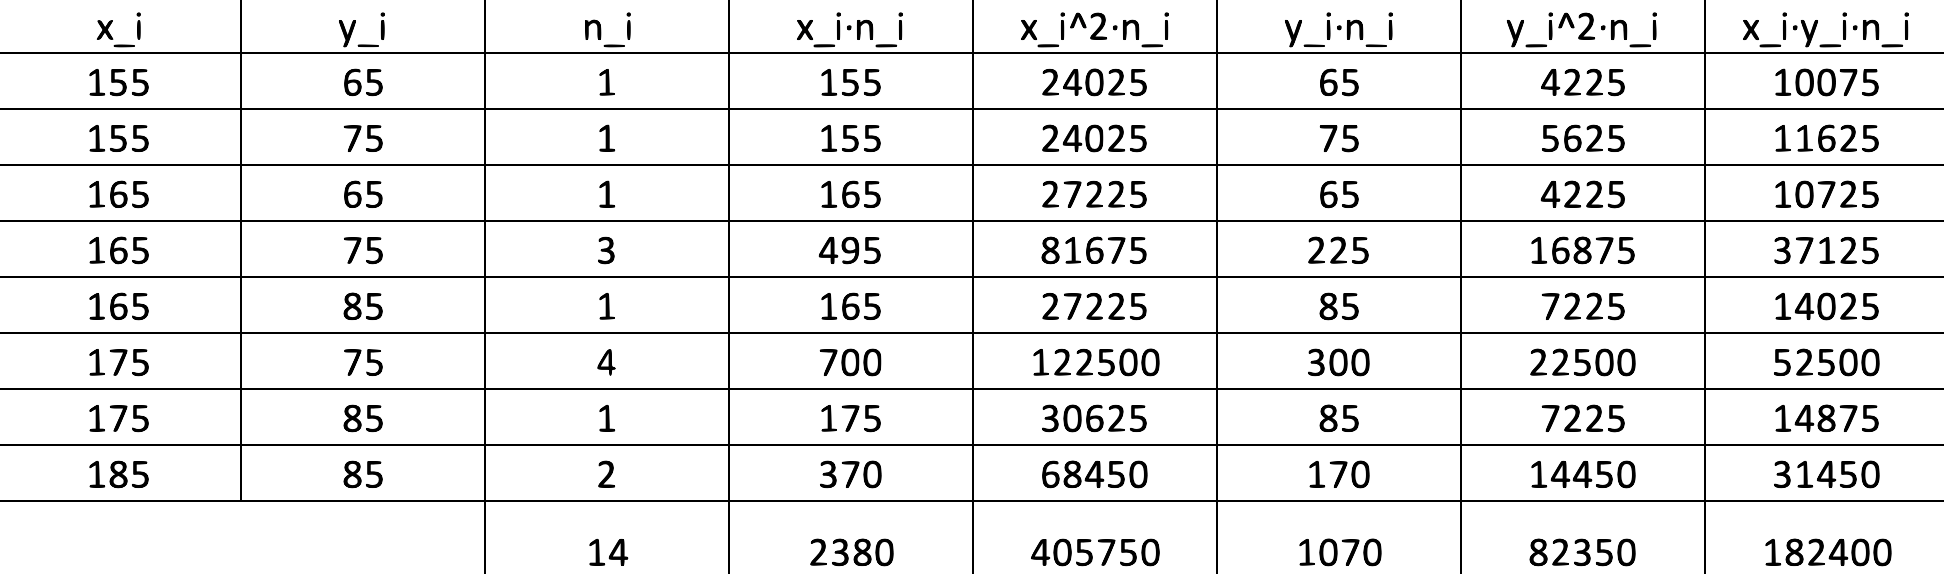
\includegraphics[width=0.95\textwidth]{imagenes/imagenes03/T03IM04.png}
	\end{figure}

\begin{multicols}{2}
$\bar x=\dfrac{2380}{14}=170$

$\quad$

$s_x=\sqrt{\dfrac{405750}{14}-170^2}=9.06$

$\bar y=\dfrac{1070}{14}=76.43$	

$\quad$

$s_y=\sqrt{\dfrac{82350}{14}-76.43^2}=6.37$
\end{multicols}
$$s_{xy}=\dfrac{182400}{14}-170\cdot 76.43=35.47$$

\end{example}


\section{Dependencia o Correlación}


En cursos de Análisis Matemático se estudian relaciones \emph{determinísticas}, si dos variables x e y están relacionadas de esa manera, sabiendo el valor de x, podemos conocer exactamente el valor de y.

En muchas aplicaciones encontramos variables que parecen estar relacionadas, aunque no de manera determinística. Esto significa que, saber el valor de una variable (la variable explicativa) no nos permite conocer exactamente el valor de la otra (la variable respuesta), ya que  ésta puede considerarse una variable aleatoria. Por ejemplo, sean `x' la edad de un niño e `y' su talla, sabemos que la talla depende de la edad, pero también depende de muchas otras condiciones; para una determinada edad, la talla puede considerarse como una variable aleatoria. Cuando ocurre esto decimos que las variables están \textbf{correlacionadas}, son estadísticamente dependientes.

\begin{definition}
.	Entre dos variables estadísticas existe \textbf{dependencia estadística o \emph{correlación}} cuando los valores que toma una de ellas están relacionados con los valores que toma la otra, pero no de manera exacta.	

La relación existente entre dos variables queda reflejada en los diagramas de dispersión o nubes de puntos de la distribución bidimensional.

--- Si los puntos de la nube se sitúan sobre una recta o una curva cuya expresión matemática podemos determinar, hablaremos de dependencia funcional entre las variables X e Y.

--- Si los puntos de la nube se agrupan en torno a una posible recta, o curva, no muy definida pero reconocible, hablaremos de dependencia estadística o correlación entre las variables X e Y.

--- Si los puntos de la nube no se agrupan en torno a ninguna curva, están completamente en desorden, hablaremos de independencia entre las variables X e Y.

	\begin{figure}[H]
			\centering
			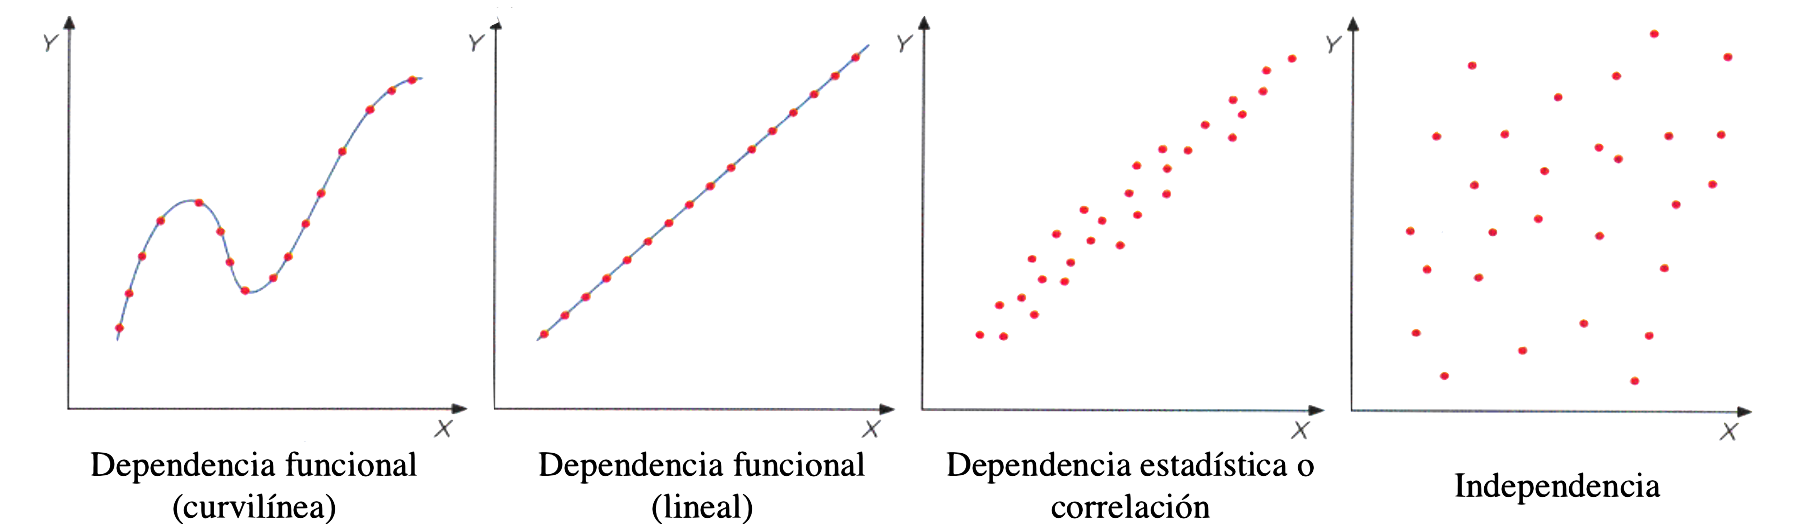
\includegraphics[width=0.95\textwidth]{imagenes/imagenes03/T03IM06.png}
			\caption*{\scriptsize{https://yoquieroaprobar.es/\_pdf/04140.pdf}}
	\end{figure}
	

\end{definition}

\section{Correlación lineal}

El caso más simple que estudiaremos en este capítulo, es el modelo de \textbf{regresión lineal}.

 El \textbf{coeficiente de correlación lineal de Pearson}, es un número \emph{adimensional} que sire para medir, de forma cuantitativa, la dependencia lineal de las variables X e Y.

\begin{definition}
.	El \textbf{coeficiente de correlación lineal} de Pearson mide una tendencia lineal entre dos variables numéricas.

\vspace{4mm} Es el método de correlación más utilizado y se necesita que:

\begin{itemize}
\item la tendencia debe ser de tipo lineal.
\item no existan valores atípicos (outliers).
\item las variables deben ser cuantitativas, si  son cualitaivas no podremos aplicar la correlación de Pearson.
\item debe haber suficientes datos (algunos autores recomiendan tener más de 30 puntos u observaciones).
\end{itemize}
Es de gran ayuda, para observar la tendencia lineal, el disponer del diagrama de dispersión o nube de puntos correspondiente.

El \textbf{coeficiente de correlación lineal}, $\boldsymbol{r}$, se define como:

$$\boxed{\ \boldsymbol{ r\ = \ \dfrac {s_{xy}}{s_x \cdot s_y} }  \ }$$

\vspace{3mm} %*****************************
\begin{itemize}
\item $\boldsymbol{-1 \ \le \ r \ \le 1}	$
\item Si $\ |r|=1 \to $ relación funcional
\item Si $\ r=0 \to $ variables incorreladas, no hay dependencia entre ellas.
\item Si $\ r>0\to $ correlación positiva o directa; Si $\ r<0\to $ correlación negativa o inversa.
\item Si $\ |r|\approx 1 \to $ correlación muy fuerte.
\end{itemize}

\vspace{5mm} %*****************************
	\begin{figure}[H]
			\centering
			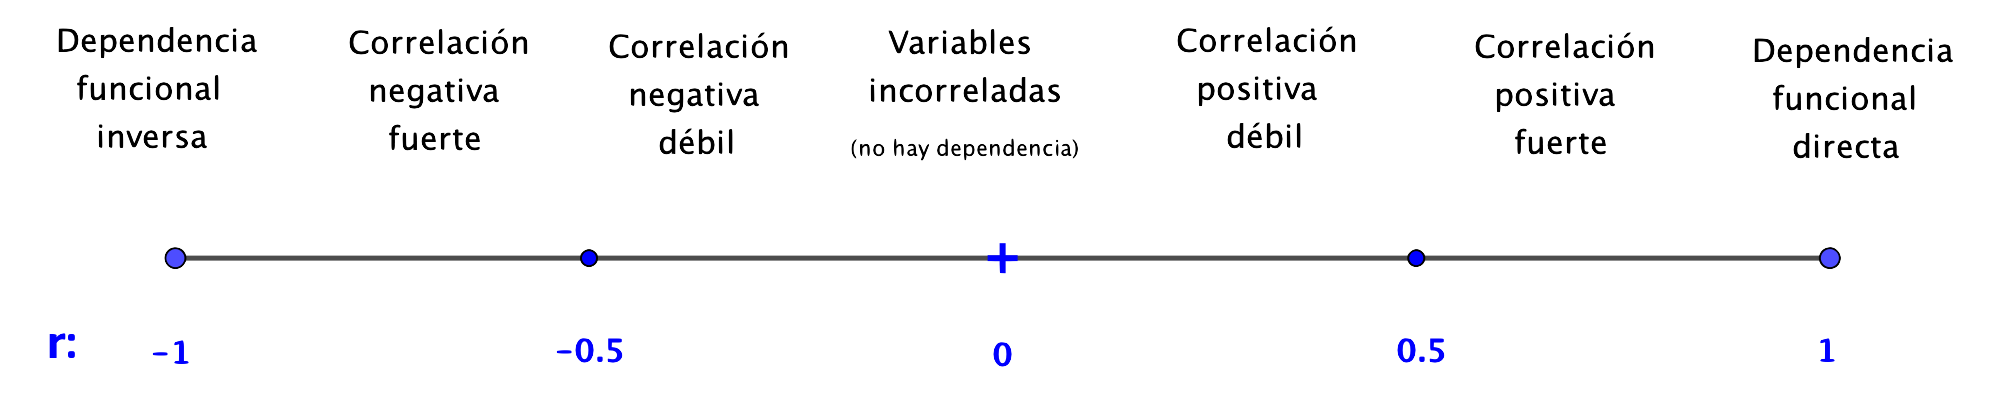
\includegraphics[width=0.95\textwidth]{imagenes/imagenes03/T03IM07.png}	
		\end{figure}
		

\vspace{5mm} \underline{Coeficiente de correlación y diagrama de dispersión:}

\vspace{5mm} %*****************************
		\begin{figure}[H]
			\centering
			\includegraphics[width=0.95\textwidth]{imagenes/imagenes03/T03IM05.png}
			\caption*{\scriptsize{imagen de https://www.maximaformacion.es/blog-dat/que-es-la-correlacion-estadistica-y-como-interpretarla/}}
	\end{figure}
\end{definition}

\vspace{10mm} %*****************************
\begin{multicols}{2}
\underline{Observación} 

No es suficiente el cálculo del coeficiente de correlación para negar la dependencia entre dos variables. Puede haber casos en que $r=0$ y sin embargo existir un tipo de dependencia (aunque no lineal) entre las variables.

	\begin{figure}[H]
			\centering
			\includegraphics[width=0.3\textwidth]{imagenes/imagenes03/T03IM10.png}
	\end{figure}
\end{multicols}

	
\section{Regresión lineal}

\begin{theorem}
.	Dada la variable estadística bidimensional $(x_i, \ y_i; \ n_{ij})$ \textcolor{gris}{($(x_i,\ y_i,\ n_i) $, en tablas de entrada simple))}, si el diagrama de dispersión indica una dependencia lineal y el coeficiente de correlación lineal confirma una correlación fuerte, la \emph{recta} $y=a+bx$ que mejor se ajusta a la nube de puntos es la \textbf{recta de regresión}, de ecuación:

$$ \boxed{\ \  \boldsymbol{ y-\bar y \ =\  \dfrac {s_{xy}}{s_x^2}\  (\ x-\bar x\ ) }\ \  }$$
\end{theorem}

\begin{proof}\textcolor{white}{.}

	Para encontrar esta expresión usaremos el \textbf{método de los mínimos cuadrados}.

\begin{multicols}{2}
$\quad$

% Please add the following required packages to your document preamble:
% \usepackage{multirow}
\begin{table}[H]
\centering
\begin{tabular}{c|c|c|c}
\multirow{2}{*}{\begin{tabular}[c]{@{}c@{}}Variable\\ estad. 2dim\end{tabular}} & $\boldsymbol {x_i}$ & $\boldsymbol {y_i}$ & $\boldsymbol {n_i}$ \\ \cline{2-4} 
 & $\cdots$ & $\cdots$ & $\cdots$
\end{tabular}
\end{table}


$$ y\ =\ a\ +\ bx$$

$$y_{ri}=a+bx_i;\qquad d_i=y_i-y_{ri}$$

$\quad$
	\begin{figure}[H]
			\centering
			\includegraphics[width=0.5\textwidth]{imagenes/imagenes03/T03IM08.png}
	\end{figure}
\end{multicols}

El \emph{método de los mínimos cuadrados} consiste en encontrar los coeficientes $\boldsymbol{a}$ y $\boldsymbol{b}$ de la recta $\boldsymbol{y=a+bx}$ tal que la suma de los cuadrados de las distancias, $D$, da cada punto a la recta sea \textbf{mínima}. Una vez encontrada esta recta, recibe el nombre de \textbf{recta de regresión}.


$D=d_1^2+d_2^2+\cdots +d_N^2=\displaystyle  \sum_{i=1}^N \ d_i^2 = \sum_{i=1}^N \ [\ y_i-(a+bx_i)\ ]^2$
Puesto que $D=D(a,b)$, por análisi matemático sabemos que el mínimo ha de verificar que las derivadas de $D$ sean cero: $\displaystyle \pdv{D}{a}=\pdv{D}{b}=0$

\vspace{3mm} $\begin{cases}
\ \ \displaystyle \pdv{D}{a}\ =\ -2 \sum_{i=1}^N\ [ \  y_i-(a+bx_i)  \ ]	 \ = \ 0
\\
\ \ \displaystyle \pdv{D}{b}\ =\ -2 \sum_{i=1}^N\ [ \  y_i-(a+bx_i)  \ ]\cdot x_i	 \ = \ 0
\end{cases}$

\vspace{3mm} $\to \ \begin{cases}
\ \ \displaystyle   \sum_{i=1}^N\ y_i - Na - b\sum_{i=1}^N \ x_i \ = \ 0
\\
\ \ \displaystyle   \sum_{i=1}^N\   y_i\cdot x_i - a\sum_{i=1}^N\ x_i - b\sum_{i=1}^N\ x_i^2	 \ = \ 0
\end{cases}$


\vspace{3mm} Dividiendo por $N$, 
$\quad \begin{cases}
\ \ \bar y - a - b\bar x=0 
\\ 
\ \  \dfrac{\displaystyle \sum_{i=1}^N\ x_i\ y_i}{N} - a\bar x - b \dfrac {\displaystyle \sum_{i=1}^N\ x_i^2}{N}
\end{cases} \ \to \ 
\begin{cases}
\ \ a=\bar y - b \bar x \\ 
\\ s_{xy}+\bar x\ \bar y-a\bar x-b(s_x^2+{\bar x}^2) 	
\end{cases}$

\vspace{3mm} Resolviendo el sistema, $\ \ \begin{cases}
\ \ a=\bar y - \dfrac{s_{xy}}{s_x^2} \ \bar x \\ \ \ b=\dfrac{x_{xy}}{s_x^2}	\end{cases}$, con lo que la recta de regresión buscada es:

$\subrayado{\  \boxed { \ \boldsymbol{ y-\bar y \ = \ \dfrac{s_{xy}}{s_x^2}\ (x-\bar x) } \ } \ } \quad $ \textbf{Recta de regresión de Y sobre X}. 

A la pendiente,  $\boldsymbol{ \ \dfrac{s_{xy}}{s_x^2}\ = \ m_{YX} \  }$, se le llama \textbf{coeficiente de regresión de Y sobre X}. Y es la variable dependiente (explicada) y X es la variable independiente (explicativa). 

La \emph{recta de regresión de Y sobre X} sirve para \emph{hacer predicciones sobre la Y sabida la X}. Si lo que deseamos es \emph{hacer predicciones sobre la X sabida la Y}, necesitaremos la \emph{recta de regresión de X sobre Y}, que se obtiene de modo análogo a la anterior pero considerando ahora la X como variable dependiente (explicada) y la Y como variable independiente (explicativa). Es decir, intercambiando los papeles de X e Y:

$\subrayado{\  \boxed { \ \boldsymbol{ x-\bar x \ = \ \dfrac{s_{xy}}{s_y^2}\ (y-\bar y) } \ } \ } \quad $ \textbf{Recta de regresión de X sobre Y}. 

A la pendiente,  $\boldsymbol{ \ \dfrac{s_{xy}}{s_y^2}\ = \ m_{XY} \  }$, se le llama \textbf{coeficiente de regresión de X sobre Y}. X es la variable dependiente (explicada) e Y es la variable independiente (explicativa).

\end{proof}

\begin{definition}
.	Hay pues dos rectas de regresión:

$$\subrayado{\  \boxed { \ \boldsymbol{ y-\bar y \ = \ \dfrac{s_{xy}}{s_x^2}\ (x-\bar x) } \ } \ } \quad  \textbf{Recta de regresión de Y sobre X}.$$ 

$$\subrayado{\  \boxed { \ \boldsymbol{ x-\bar x \ = \ \dfrac{s_{xy}}{s_y^2}\ (y-\bar y) } \ } \ } \quad  \textbf{Recta de regresión de X sobre Y}. $$

La primera sirve para hacer predicciones sobre los valores de Y mientas que la segunda se usa para hacer predicciones sobre la X.	
\end{definition}

\begin{theorem}
.	$$ r\ = \ \dfrac{s_{xy}}{s_x\cdot s_y} \ = \ \pm \sqrt{m_{YX}\cdot m_{XY}}	$$

El signo de $r$ coincide con el de $s_{xy}$.
\end{theorem}

\vspace{-5mm} %***************************
\begin{proof}\textcolor{white}{.}

Evidente, $\ \dfrac{s_{xy}}{s_y^2}\ = \ m_{XY};\quad \dfrac{s_{xy}}{s_x^2}\ = \ m_{YX} $, por lo que	$\ m_{YX}\cdot m_{XY}=\dfrac{s_{xy}}{s_y^2}\  \dfrac{s_{xy}}{s_x^2}=r^2$
\end{proof}

\begin{theorem}
.	Propiedades de las dos rectas de regresión.

\begin{itemize}

\item Las dos rectas de cortan en el punto $(\bar x, \bar y)$, llamado \emph{centro de gravedad} de la nube de puntos (diagrama de dispersión).

\item Las pendientes de las dos rectas $m_{YX}$ y $m_{XY}$ tienen el mismo signo, que a su vez es igual al signo del coeficiente de correlación lineal $r$. Dicho signo lo dicta el de la covarianza $s_{xy}$.

\item En los casos en los que tenemos correlación perfecta (funcional), $r=\pm 1$, ( XY XY ), las dos rectas de regresión coinciden. De no ser así, forman un determinado ángulo que es mayor cuando menor es la correlación, siendo máximo ($90^o$) cuando las variables son incorreladas, $r=0$, en este caso las rectas son perpendiculares ($x=\bar x;\ y=\bar y$).

	\begin{figure}[H]
			\centering
			\includegraphics[width=0.6\textwidth]{imagenes/imagenes03/T03IM09.png}
	\end{figure}
\end{itemize}
\end{theorem}

\section{Coeficiente de determinación}

\textbf{\emph{El coeficiente de determinación mide la bondad del ajuste de la recta de regresión}}

\vspace{5mm} %****************************
\begin{definition}
	
El coeficiente de correlación lineal indica el grado de linealidad entre las dos variables, pero para analizar la bondad del ajuste de la recta de regresión se utiliza un parámetro nuevo llamado \textbf{coeficiente de determinación}, $\boldsymbol{ r^2 }$, indica el porcentaje de la variación de Y que puede ser explicada por X y, también, de la X respecto de la Y puesto que $r^2$ coincide coincide para las dos rectas de regresión:
$\ \ r^2 \ = \ \dfrac{s_{xy}^2}{s_x^2\cdot s_y^2} \ = \ m_{XY}\cdot m_{YX}$

Como $0 \le r^2 \le  1$, la interpretación de esta medida es similar a la de $r$:

\begin{itemize}
\item Si $r^2 = 0$, significa que no existe tal relación lineal entre las variables (puede existir otro tipo de relación o no haber ninguna entre las dos variables, incorreladas). No tendría sentido utilizar las rectas de regresión para analizar la influencia de X sobre Y, ni para predecir el valor de Y, dado X.

\item Si $r^2 = 1$, significa que el ajuste es perfecto (funcional). Las rectas pasan por todos los puntos de la nube, obviamente porque éstos están alineados y proporcionan toda la información sobre el comportamiento de Y en función de X, así como de X para Y,para la muestra considerada.

\item Si $0 < r^2 < 1$, habrá una determinada correlación lineal entre las variables, mayor cuanto más se aproxime a uno el coeficiente de determinación. Como $r^2$ , indica el \emph{porcentaje de la variación de Y que puede ser explicada por X} o al revés, un valor concreto de $r^2$ se puede interpretar en los siguientes términos: si $r^2 =0,92$, por ejemplo,  significa que las rectas obtenidas explican en un 92\% el comportamiento de una variable en función de la otra. El 8\% restante de la variación puede deberse al azar o a la influencia  de otras variables distintas.
\end{itemize}

\end{definition}


	

\vspace{15mm} %************************************
\begin{adjustwidth}{25pt}{25pt}
	\textcolor{gris}{\rule{70mm}{0.1mm}}
\vspace{5mm} %************************************
	\begin{destacado}
	Un coeficiente de determinación alto implica la relación lineal entre las variables es fuerte, pero eso no tiene por qué implicar que los cambios en una variable se expliquen por la otra variable. Así, si consideramos la variable (X,Y) en que X representa los ingresos mensuales de una muestra de 100 familias de una determinada ciudad e Y representa la asignación media asignada a sus hijos, el cambio brusco en los ingresos mensuales de una familia puede explicar un descenso de la asignación que dan a sus hijos, pero un descenso en la asignación a los hijos no explica el cambio en los ingresos de la familia (podría ser un castigo).
	
	Si existe una relación causal entre dos variables, la correlación por sí misma no nos dice nada sobre la dirección de la causalidad.
	\begin{flushright}
		\textit{\textbf{Correlación no implica causalidad.}}
	\end{flushright} 
	\end{destacado}
	\begin{flushright}
	\rule{70mm}{0.1mm}	
	\end{flushright}
\end{adjustwidth}
\vspace{1cm}

\subsection{Valoración de las predicciones. Interpolación y extrapolación}

\begin{definition}
	
La recta de regresión nos permite predecir valores de una variable a partir de los de la otra. No obstante, hay que tener siempre presente que existen las siguientes limitaciones:

\begin{itemize}
\item Las predicciones realizadas a partir de una recta de regresión no son fiables si entre X e Y no hay un alto grado de correlación lineal, es decir, si r no es, en valor absoluto, cercano a 1.
\item Las predicciones deben hacerse con valores próximos a los pares considerados. Las estimaciones obtenidas para valores próximos al centro de gravedad de la distribución son más fiables que las obtenidas para valores muy alejados de él. 
\item Los valores que están dentro del rango de la variable explicativa son interpolaciones; las que están fuera, extrapolaciones. Extrapolar siempre supone un riesgo añadido, la variable explicada puede tener una dependencia lineal con la variable explicativa en el rango de valores, pero no tenerlo o no ser lineal fuera de este rango.
\item La fiabilidad de una recta de regresión es mayor cuanto mayor sea el número de datos considerados para calcularla, N.	
\item Se considera buena la predicción si $r^2>75\%$ y muy buena a partir de $r^2>90\%$. Si $r^2<60\%$, las predicciones serán poco fiables.
\end{itemize}
\end{definition}


\vspace{1cm} %***************************************
	\begin{figure}[H]
			\centering
			\includegraphics[width=0.6\textwidth]{imagenes/imagenes03/T03IM11.png}
	\end{figure}
\vspace{1cm} %***************************************

\begin{example}
.	Siguiendo con el ejemplo que nos ocupa en todo el tema:

	\begin{table}[H]
\centering
\begin{tabular}{c|c|c|c|c}
$\boldsymbol{\downarrow Y \ \ / \ \ X \rightarrow}$ & \textbf{{[}60,70{[}$\to 65$} & \textbf{{[}70,80{[}$\to 75$} & \textbf{{[}80,90{[}$\to 85$} & \textbf{$n_{x_i}$} \\ \hline
\textbf{{[}150,160{[}$\to 155$} & 1 & 1 & 0 & 2 \\ \hline
\textbf{{[}160,170{[}$\to 165$} & 1 & 3 & 1 & 5 \\ \hline
\textbf{{[}170,180{[}$\to 175$} & 0 & 4 & 1 & 5 \\ \hline
\textbf{{[}180,190{[}$\to 185$} & 0 & 0 & 2 & 2 \\ \hline
\textbf{$n_{y_j}$} & 2 & 8 & 4 & \textbf{14}
\end{tabular}
\end{table}


	\begin{figure}[H]
			\centering
			\includegraphics[width=0.95\textwidth]{imagenes/imagenes03/T03IM02.png}
	\end{figure}

$\qquad \bar x=\dfrac{2380}{14}=170;$$\quad$$s_x=\sqrt{\dfrac{405750}{14}-170^2}=9.06$

$\qquad \bar y=\dfrac{1070}{14}=76.43;$$\quad$$s_y=\sqrt{\dfrac{82350}{14}-76.43^2}=6.37$

$\qquad s_{xy}=\dfrac{182400}{14}-170\cdot 76.43=35.47$

\textcolor{green}{\rule{100mm}{0.1mm}}
	
\vspace{3mm} %**********************
Calcula el coeficiente de correlación lineal y el coeficiente de determinación. ?`Cómo es la dependencia de estas variables?

?`Cuál es el valor que debería tener la variable Y para un valor de X=77 Kg? ?Qué debería valer ya X si la Y=210 cm? ?`Cómo de fiables son estas predicciones?

\vspace{-3mm} \begin{center}\textcolor{green}{\rule{100mm}{0.1mm}}\end{center}

Ala vista del diagrama de dispersión, intuimos que va a haber una correlación positiva y débil. Calculemos el coeficiente de correlación:

\vspace{2mm} $r=\dfrac{s_{xy}}{s_x\cdot s_y}=\dfrac{35.47}{9.06\cdot 6.37}=0.61 \to$ correlación positiva y débil, no tiene demasiado sentido hacer predicciones.

\vspace{2mm} $r^2=0.61^2=0.38=38\%$, las predicciones explicarían el 38\% de los valors, el 63\% restante no.

\vspace{2mm} Aunque la correlación indica que las predicciones no serán fiables, vamos a hacerlas ya que las piden:

\vspace{2mm} --- Recta de regresión de X sobre Y:  $\ x-\bar x=\dfrac{s_{xy}}{s_y^2}(y-\bar y)$.

\vspace{2mm} $x-170=\dfrac{35.47}{6.37^2}(y-76.43) \ \to \ x=0.87y+103.19$

\vspace{2mm} Para un $y=77$ kg, obtenemos una $y=170.18$ cm.

\vspace{2mm} --- Recta de regresión de Y sobre X: $\ y-\bar y=\dfrac{}s_{xy}{x_x^2}(x-\bar x)$.

\vspace{2mm} $y-76.43=\dfrac{35.47}{9.06^2}(x-170) \ \to \ y=0.43x+2.97$

\vspace{2mm} Para una $x=210$ cm, obtenemos un $y=77$ Kg.

\vspace{2mm} Ya hemos advertido que las previsiones no son fiables dado que la correlación es débil (r=0.61). Aún así, la segunda previsión es mucho menos fiable que la primera pues se trata de una \emph{peligrosa} extrapolación, una altura de 210 cm está fuera de nuestro rango de valores, [150,190[.

En la siguiente figura mostramos las dos rectas de regresión así como las predicciones efectuadas. Obsérvese como la segunda predicción es una extrapolación.

\vspace{1cm} %***************************************
 
	\begin{figure}[H]
			\centering
			\includegraphics[width=0.75\textwidth]{imagenes/imagenes03/T03IM12.png}
	\end{figure}

\end{example}

\vspace{2cm} %***************************************

\begin{ejemplo}
\begin{ejre}
Las notas obtenidas en Matemáticas y Física por cinco alumnos son:

\begin{table}[H]
\centering
\begin{tabular}{l|rrrrr}
\textbf{Matemáticas (X)} & $\qquad 6$ &  $\ \ 4$ &  $\ \ 8$ &  $\ \ 5$ &  $\ \ 3.5$ \\ \hline
\textbf{Física (Y)} & $6.5$ & $4.5$ & $7$ & $5$ & $4$
\end{tabular}
\end{table}

\begin{adjustwidth}{20pt}{10pt}
\begin{enumerate}[a) ]
\item Dibujar el diagrama de dispersión y comentar si se espera o no que haya correlación lineal.
\item Calcular e interpretar los coeficientes de correlación lineal y de determinación.
\item Escribir las dos rectas de regresión.
\item Para una alumno de ese grupo que saque	 un 7.5 en matemáticas, ?`qué nota se espera que obtenga en física?
\item Si una alumno obtiene un 9 en física, ?cuál debería ser su nota en matemáticas?
\item Qué fiabilidad merecen las predicciones anteriores.
\end{enumerate}
\end{adjustwidth}
\vspace{5mm}

	\begin{figure}[H]
			\centering
			\includegraphics[width=0.75\textwidth]{imagenes/imagenes03/T03IM13.png}
	\end{figure}
--- a) A la vista de la nube de puntos, se espera una correlación positiva (o directa) y fuerte.

Se han incluído en el dibujo	 las dos rectas de regresión y en cdg centro de gravedad, $(\bar x, \bar y)$, de la nube de puntos (punto rojo).

--- b) y c). Cálculo de parámetros de la distribución bidimensional. Todos las frecuencias son 1, y N=5.

Con una sencilla hoja de cálculo obtenemos: $\Sigma x=26.5$, $\Sigma y=27$, $\Sigma x^2=153.25$, $\Sigma y^2=152.5$, $\Sigma x\cdot y=152$, por lo que:

$\bar x=5.3$; $s_x=1.6$; $\quad \bar y=5.4$; $s_y=1.16$; $\qquad s_{xy}=1.78$

De ahí: $\quad r=0.96; \qquad r^2=0.92=92\%$

Al ser $r=0.96$, la correlación es directa (positiva) y fuerte, habrá un alto grado de fiabilidad en las predicciones (ojo con las extrapolaciones). Por ser $r^2=92\%$, el $92\%$ de la nota de física es explicada por la de matemáticas y viceversa.

Las rectas de regresión son : $\quad y=0.695x+1.715; \qquad x=1.323y-1.843$

--- d), e) y f): predicciones.

$x=7.5 \to \textcolor{gris}{y=0.695x+1.715} \to y=6.93$

La predicción es altamente fiable dado el elevado coeficiente de correlación y el que se trata de una interpolación, $7.5\in [3.5,8]$

$y=9 \to \textcolor{gris}{x=1.323y-1.843} \to x=10.06$

La predicción es fiable por el elevado coeficiente de correlación pero arriesgada al tratarse de una extrapolación, $9\notin [4,7]$

\vspace{4mm} \textsf{De todos modos, el número de datos $N=5$ es muy pequeño para garantizar que las predicciones  tengan la fiabilidad necesaria.}
\end{ejre}	
\end{ejemplo}


\section{Recta de Tukey}

\begin{definition}
.	\vspace{2mm} La \textbf{recta de Tukey o recta mediana-mediana}	
permite ajustar una recta a una nube de puntos en algunos casos en los que el ajuste mínimo cuadrático produce resultados no muy buenos. La recta de Tukey o Mediana-Mediana es un método novedoso y práctico que puede venir a apoyar al que  hemos visto de  \emph{mínimos cuadrados} o \emph{recta de regresión}.

\vspace{2mm} La recta de Tukey\footnote{John Wilder Tukey (16 de junio de 1915 - 26 de julio de 2000). Estadístico estadounidense. Introdujo, además, los diagramas de cajas y bigotes.} es un método ingenioso que no requiere de un fundamento matemático demasiado abstracto en su tratamiento.

\vspace{2mm} Se utiliza cuando hay valores extraños (outliers) que, como sabemos, afectan mucho a las medias. Veremos como se calcula en el siguiente \textbf{ejemplo}.

\end{definition}

\begin{example}
.	Considera la siguiente distribución, dibuja la nube de puntos, la recta de regresión de Y sobre X y la recta de Tukey.

\begin{table}[H]
\centering
\begin{tabular}{l|rrrrrrrrrrrr}
\textbf{X} & 1 & 2 & 3 & 5 & 6 & 7 & 8 & \textcolor{red}{9} & 10 & 12 & 14 & \textcolor{red}{21} \\ \hline
\textbf{Y} & 9 & 11 & 13 & 13 & 15 & 14 & 16 & \textcolor{red}{1} & 16 & 14 & 19 & \textcolor{red}{2}
\end{tabular}
\end{table}
Hemos puesto en rojo los valores \emph{extraños}. Se ven a simple vista en el diagrama de dispersión.

	\begin{figure}[H]
			\centering
			\includegraphics[width=0.75\textwidth]{imagenes/imagenes03/T03IM14.png}
	\end{figure}
Como se puede observar, la recta de regresión (morada) se ajusta muy mal al diagrama de dispersión. En cambio, la recta de Tukey se ajusta mejor, sobre todo si obviamos mentalmente los puntos que están muy aislados de la nube (los señalados en rojo en la tabla).	
	
\vspace{2mm} Se deja como ejercicio para el/la lector/a el encontrar la recta de regresión de Y sobre X: $\ y=0.16x+13.57$

\vspace{5mm} \underline{Vamos con la recta de Tukey}:

 
\begin{enumerate}
\item Se ordenan los datos en orden creciente de las abcisas (ya lo tenemos).
\item Se divide el conjunto de datos ordenados en tres grupos:

$\qquad G1=\{(1,9),\ (2,11),\ (3,13),\ (5,13) \}$

$\qquad G2=\{(6,15),\ /7,14),\ (8,16),\ (9,1) \}$

$\qquad G3=\{(10,16),\ (12,14),\ (14,19),\ (21,2) \}$



\item Para cada grupo $G_i$ se calculan las medianas de las abcisas (x) y de las ordenadas (y) del grupo, $me_{x_i}$ y $me_{y_i}$.


$G1: \ \left.
\begin{cases}
\quad \text{Abcisas   G1:} & 1,\ 2,\ 3,\ 5 \ \ \to \ m_{x_1}=2.5	 \ 
\\
\quad \text{Ordenadas G1:} & 9, 11, 13, 11 \ \to \ m_{y_1}=12	\ 
\end{cases} \ \right\}  \quad  \Rightarrow \ P1(2,5,12) $

$G2: \ \left.
\begin{cases}
\quad \text{Abcisas   G2:} & 6,\ 7,\ 8,\ 9 \ \ \to \ m_{x_1}=7.5	
\\
\quad \text{Ordenadas G2:} & 1, 14, 15, 16 \ \to \ m_{y_1}=14.5	
\end{cases} \ \right\}  \quad  \Rightarrow \ P1(7,5,14.5) $

$G2: \ \left.
\begin{cases}
\quad \text{Abcisas   G3:} & 10, 12, 14, 21 \ \ \to \ m_{x_1}=13 	
\\
\quad \text{Ordenadas G3:} & 2, 14, 16, 29 \ \ \ \to \ m_{y_1}=15	
\end{cases} \ \right\}  \quad  \Rightarrow \  P1(13,15) $

\vspace{2mm} Obsérvese que el número de datos en este caso es N = 12, múltiplo de 3, y, por tanto, cada grupo está formado por 4 datos. 

\vspace{2mm} Si el número de datos N no es múltiplo de 3, puede ocurrir que:

--- Sea múltiplo de 3 más 1; en este caso, el grupo G2 se deja con un dato más.

--- Sea múltiplo de 3 más 2; en este caso, el grupo G2 se deja con un dato menos, se añaden un dato más a los grupos G1 y G3.

\item \textbf{La recta de Tukey para por el baricentro del triángulo $P1P2P3$ y tiene por pendiente la de la recta que pasa por $P1$ y por $P3$}.

\vspace{2mm}  Baricentro: $B_{P1P2P3}=\dfrac{P1+P2+P3}{3}=(7.67,13.83)$

\vspace{2mm}  Pendiente: $m_{P1P3}=\dfrac{15-12}{13-2.5}=0.29$

\vspace{2mm}  Luego, la \underline{recta de Tukey} es: $\ \boldsymbol{y=0.29x+13.83}$

\end{enumerate}
\end{example}



\begin{myalertblock}{Regresiones no lineales}


El modelo de regresión lineal, estudiado para detectar dependencia lineal entre las variables, también se puede aplicar para detectar otros tipos de dependencia no lineales, como la exponencial o la potencial.

\begin{theorem}
.	\textbf{Dependencia exponencial}

Si dos variable se sospecha que están relacionadas por un modelo exponencial: $\ y=ke^{ax}$, tomando logaritmos: $\ \ln y=ax+b$, con $\ k=e^b\ \textcolor{gris}{(b=\ln k)}$.

Para encontrar una dependencia exponencial en una serie de datos $(x_i, y_i, n_i)$, buscaremos una dependencia lineal en la serie $(x_i, \ln y_i, n_i)$. Si la dependencia lineal es $Y=aX+b$, la dependencia exponencial será $Y=Ke^{aX}$, con $K=e^b$
\end{theorem}

\begin{example}
. Encontar la dependencia exponencial para los siguientes datos (X habitantes del mundo, en millones; Y año):

\begin{table}[H]
\centering
\begin{tabular}{l|rrrrrr}
X & 1750 & 1800 & 1850 & 1900 & 1950 & 2000 \\ \hline
Y & 728 & 949 & 1171 & 1608 & 2516 & 5923
\end{tabular}
\end{table}

Cálculos: 

$\ \Sigma x=11250;\ \Sigma y=12895;\ \sigma x^2=21137500;\ \Sigma y^2=46799675;\ \Sigma x\cdot y=24955950$

$\bar x=1875;\ s_x=85.39;\quad \bar y=2149.17;\ s_y=1783.54; \qquad s_{xy}=129631.25$

$r=0.85;\qquad $ Recta de regresión de Y sobre X: $\ y=17.78x-31183.33$

\vspace{4mm} Tomando logaritmos en la población (Y):

Ahora, $\ \Sigma y=43,33;\ \Sigma y^2= 314.01;\ \Sigma x\cdot y=81450.40$

Luego $\bar y=7.22;\ s_y=0.45; \ s_{xy}=37.58$

$r=0.98$. Recta de regresión de ln Y sobre X: $\ \ln y=0.0052x-7.69$

\vspace{4mm} Por último, la dependencia exponencial será: 

$y=e^{0.0052x-7.69}=e^{0.0052x}\cdot e^{-7.69}=0.00046 e^{0.0052 x}$


	\begin{figure}[H]
			\centering
			\includegraphics[width=0.95\textwidth]{imagenes/imagenes03/T03IM15.png}
			\caption*{\textcolor{gris}{\footnotesize{Ejemplo tomado de ``https://yoquieroaprobar.es/\_pdf/04140.pdf''}}}
	\end{figure}
\end{example}

\begin{theorem}
.	\textbf{Dependencia potencial}

\vspace{2mm} Si dos variables estadísticas X e Y están relacionadas por un modelo potencial: $\ y=k\ a^x$, con $k > 0$, al tomar logaritmos, se obtiene:
$\ \ln y = \ln k + a ln x$ de donde se deduce que las variables ($\ln X, \ \ln Y)$ están relacionadas por un modelo lineal.

\vspace{2mm} Para encontrar dependencia potencial en una lista de datos $(x_i, y_i, n_i)$, se aplica una regresión lineal a los datos: $(\ln x_i,\ \ln yÑi,\ n_i)$.

\vspace{2mm} Si la recta de regresión es $ln Y = a \ln X + b$, entonces la dependencia potencial en los datos originales es: $y=k\ a^x$, con $k=e^b$ .	

\vspace{2mm} Veremos un \textbf{ejemplo} que aclare todo esto.
\end{theorem}

\begin{example}
.	El científico inglés Fry Richardson midió la costa oeste de Gran Bretaña con ``reglas'' de distintos tamaños, y obtuvo los siguientes datos aproximados \textcolor{gris}{(principio de los fractales)}:	

\vspace{2mm} Calcula el coeficiente de correlación para estos datos y también para los datos $(\ln X, \ln Y)$. Compara los resultados. ?Cuál es la ley que mejor describe la dependencia entre las variables X e Y?

\begin{table}[H]
\centering
\begin{tabular}{l|lcccccc}
\textbf{Tamaño de la regla (cm)} &  & 1000 & 500 & 200 & 100 & 30 & 10 \\ \hline
\textbf{Longitud de la costa (Km)} &  & 1000 & 1000 & 1200 & 1500 & 2100 & 2800
\end{tabular}
\end{table}

Para los datos $(X, Y)$, se encuentra (hágase) que $r = –0,698$. En cambio, para los datos $(\ln x, \ln y)$ tenemos que $r = 0,985$, mucho más elevado que el anterior, y la recta de regresión es: $\ln y = –0,24 \ln x + 8,446 \ \to \ $$y=e^{-0.24 \ln x +8.46}= e^{8.46}\ x^{-0.24}= 4656.4 \ x^{-0.24}$

	\begin{figure}[H]
			\centering
			\includegraphics[width=0.75\textwidth]{imagenes/imagenes03/T03IM16.png}
			\caption*{\textcolor{gris}{\footnotesize{Ejemplo tomado de ``https://yoquieroaprobar.es/\_pdf/04140.pdf''}}}
	\end{figure}

\end{example}
\end{myalertblock}


\section{Ejercicios}

$$\subrayado{\  \boxed{ \textbf{Se deberían intentar resolver los ejercicios antes de ver su resolución.} \ } \ }$$

\vspace{1cm} %******************************************

\begin{ejemplo}
\begin{ejer}\textcolor{white}{.}

Se ha hecho una encuesta a 12 personas que han tenido un accidente de tráfico, preguntando por el número de meses transcurridos e incluyendo el grupo de edad. 

Las respuestas han sido: 

Carmen, 35: [60, 70);  Teresa, 15: [50, 60);  Pilar, 12: [50, 60);  Esther, 6: [20, 30); Juan, 8: [40, 50); Jacinto, 15: [30, 40); Jesús, 24: [50, 60); Marta, 12: [30, 40); José, 28: [40, 50); Andrés, 3: [20, 30); María Jesús, 20: [40, 50); Beatriz, 16: [30, 40) 

\begin{adjustwidth}{20pt}{10pt}
\begin{enumerate}[a) ]
\item Construye la tabla correspondiente a la variable bidimensional.
\item  Representa el diagrama de dispersión. 
\item Estudia si hay correlación entre ambas variables, y determina su coeficiente de correlación lineal.	
\item Si la persona entrevistada tuviese 87 años, ?`cuántos meses es de esperar que hayan transcurrido desde su último accidente?
\item Si a un encuestado le han transcurrido 18 meses desde su último accidente, ?`qué edad es de esperar que tenga?
\item Como de fiables son tus predicciones.
\end{enumerate}
\end{adjustwidth}
\end{ejer}
\end{ejemplo}

--- a) Representamos los datos en una tabla de doble entrada:

\begin{table}[H]
\centering
\begin{tabular}{|c|c|c|c|c|c|c|c|c|c|c|c|}
\hline
\textbf{Y   \textbackslash   X} & \textbf{3} & \textbf{6} & \textbf{8} & \textbf{12} & \textbf{15} & \textbf{16} & \textbf{20} & \textbf{24} & \textbf{28} & \textbf{35} & \textbf{total} \\ \hline
\textbf{$\boldsymbol{[20,30[\to 25}$} & 1 & 1 &  &  &  &  &  &  &  &  & \textit{2} \\ \hline
\textbf{$\boldsymbol{[30,40[\to 35}$} &  &  &  & 1 & 1 & 1 &  &  &  &  & \textit{3} \\ \hline
\textbf{$\boldsymbol{[40,50[\to 45}$} &  &  & 1 &  &  &  & 1 &  & 1 &  & \textit{3} \\ \hline
\textbf{$\boldsymbol{[50,60[\to 55}$} &  &  &  & 1 & 1 &  &  & 1 &  &  & \textit{3} \\ \hline
\textbf{$\boldsymbol{[60,70[\to 65}$} &  &  &  &  &  &  &  &  &  & 1 & \textit{1} \\ \hline
\textbf{totales} & \textit{1} & \textit{1} & \textit{1} & \textit{2} & \textit{2} & \textit{1} & \textit{1} & \textit{1} & \textit{1} & \textit{1} & \textbf{12} \\ \hline
\end{tabular}
\end{table}

--- b) Diagrama de dispersión:

	\begin{figure}[H]
			\centering
			\includegraphics[width=0.75\textwidth]{imagenes/imagenes03/T03IM17.png}
	\end{figure}

Se observa cierta correlación lineal positiva y no muy fuerte.

--- c) Cálculos:

	\begin{figure}[H]
			\centering
			\includegraphics[width=0.8\textwidth]{imagenes/imagenes03/T03IM18.png}
	\end{figure}
	
$\bar x=43,3$ años; $\ \ \bar y=16.2$ meses; $\ \ s_x=12.1$; $\ \ s_y=8.9$; $\ \ s_{xy}=76.9 \ \to \ r=0.71$. Hay una correlación positiva y no muy fuerte.

--- e) Para $x=87$ años $\ \to \ $ 

Necesitamos la recta de regresión de Y sobre X: 

$y-16.17=\dfrac{76.94}{12.13^3}\ (x-43.3) \ \to \ y= 0.52x-6.48$

$x=87$ años $\ to \ y=38.76$, casi 39 meses.

--- f) Para $y=18$ meses $\ \to \ $


Necesitamos la recta de regresión de X sobre Y:

$x-43.33=\dfrac{76.94}{8.91^2}\ (y-16.17) \ \to \ x=0.97y+27.66$

$y=18$ meses $\ \to \ x=45.12$, 45 años aproximadamente.

--- g) Al no ser muy fuerte la correlación ($r=0.71$), las estimaciones que hemos hecho no son  muy fiables, siendo la primera (87 años $\to$ 39 meses) mucho menos fiable a tratarse de una extrapolación (nuestros datos abarcan edades desde 20 hasta 70 años).




\vspace{5mm} %***************************************
\begin{ejemplo}
\begin{ejer}\textcolor{white}{.}
	La recta de regresión de una variable Y respecto de la variable X es $y = 0,3x + 1$. Los valores que ha tomado la variable $x$ han sido $\{3, 4, 5, 6, 7\}$.
	
\begin{adjustwidth}{20pt}{10pt}
 \begin{enumerate}[a) ]
 	\item Determina el valor esperado de $y$ para el valor particular de $x = 3.5$.
 	\item Si los valores de la variable Y utilizados para la regresión se multiplican por 10 y se dejan los mismos valores para la variable X, determina razonadamente la nueva recta de regresión.
 \end{enumerate}
 \end{adjustwidth}
	
\end{ejer}
\end{ejemplo}

--- a) $x=3.5 \ \to \ y=0.3\cdot 3.5+1=2.05$

--- b) $Y':\ 10\cdot y_i \to \bar y'=10 \bar y$
$;\quad$
$S'_{XY}=	\dfrac {\displaystyle \sum_{i=1}^N x_i \ 10 y_i \ n_i}{N}-\bar x \cdot 10 \bar y = 10 s_{xy}$

$ y - 10 \bar y= \dfrac {10 s_{xy}}{s_x^2}\ (x-\bar x) \ \to \ 
y=10\ \dfrac{s_{xy}}{s_x^2} \ x+ 10 \left(\bar y - \dfrac {s_{xy}}{s_x^2} \right) =3x+10$


\vspace{5mm} %***************************************
\begin{ejemplo}
\begin{ejer}\textcolor{white}{.}
	Cien alumnos prepararon un examen de Matemáticas. Se representa por X el número de problemas hechos por cada alumno en la preparación, y por Y, la calificación obtenida. Sabiendo que las medias aritméticas de esas variables fueron $\bar x= 9.2$ e $\bar y= 9.5$, que el coeficiente de correlación entre esas variables fue $0.7$ y que la desviación típica de la variable Y fue el doble que la de la variable X, calcula las ecuaciones de las rectas de regresión.
\end{ejer}
\end{ejemplo}

$s_y=2s_x \ \to \ r=\dfrac{s_{xy}}{s_x\ s_y}= \dfrac{s_{xy}}{2 s_x^2}=0.7 \ \Rightarrow \ \dfrac{s_{xy}}{s_x^2}=1.4$

$y-\bar y=\dfrac{s_{xy}}{s_x^2}\ (x-\bar x) \ \ \Rightarrow \ \ y-9.5=1.4\ (x-9.2)$

$\dfrac{s_xy}{s_y^2}=\dfrac{s_{xy}}{(2s_x)^2}=\dfrac 1 4 \ \dfrac{s_{xy}}{s_x^2}=\dfrac 1 4 \ \dfrac 1.4 =0.35$

$x-\bar x=\dfrac{s_{xy}}{s_y^2}\ (y-\bar y) \ \ \Rightarrow \ \ x-9.2=0.35\ (y-9.5)$





 
\subsection{Problemas propuestos (con solución)}



\begin{adjustwidth}{20pt}{10pt}
\begin{enumerate}[PB. 1. ]

\item En cada uno de estos casos debes decir si, entre las dos variables que se citan, hay relación funcional o estadística (correlación) y, en este último caso, indicar si es positiva o negativa:

	\begin{enumerate}[a) ]
	\item En un conjunto de familias: estatura media de los padres -- estatura media de los hijos.
	\item Entre los países del mundo respecto a España: volumen de exportación -- volumen de importación.
	\item En los países del mundo: tasa de mortalidad infantil -- médicos por cada 1 000 habitantes.
	\item En las viviendas de una ciudad: kw consumidos en un mes -- coste del recibo de la luz.
	\item En los equipos de fútbol: posición al finalizar la liga -- número de partidos perdidos.
	\end{enumerate}

\hspace{-1cm}\rotatebox{180}{\leftline{\textcolor{gris}{E+, E-, E-, F+, E+}}}\vspace{1cm}



\item Dados los coeficientes de correlación: $\ r_1=0.64; \ r_2=0.95;\ r_3=-1; \ r_4=-0.76$; asocia cada uno de ellos a las siguientes nubes de puntos.

	\begin{figure}[H]
			\centering
			\includegraphics[width=0.95\textwidth]{imagenes/imagenes03/T03IM19.png}
	\end{figure}
 
\hspace{-1cm}\rotatebox{180}{\leftline{\textcolor{gris}{$r_1\to C;\ r_2\to B;\ r_3\to A;\ r_4\to D$}}}\vspace{1cm}





\item Dados los coeficientes de regresión $\ r_1=-0.9;\ r_2=0.99;\ r_3=0.6;\ r_4=-0.2;\ r_5=-0.5; \ r_6=0.1$ y las rectas de regresión de la siguiente figura, asocia por parejas.

\begin{figure}[H]
			\centering
			\includegraphics[width=0.95\textwidth]{imagenes/imagenes03/T03IM20.png}
	\end{figure}

 
\hspace{-1cm}\rotatebox{180}{\leftline{\textcolor{gris}{$I\to r_3;\ II\to r_6;\ III\to r_1;\ IV\to r_5;\ V\to r_2;\ VI\to r_4$}}}\vspace{1cm}





\item Un excursionista, en diez marchas distintas, toma las siguientes medidas: x -- altura de lugar (en m); y -- presión atmosférica (en mm Hg); z -- número de pulsaciones en reposo.

\begin{table}[H]
\centering
\begin{tabular}{|c|r|r|r|r|r|r|r|r|r|r|}
\hline
\textbf{x} & 0 & 184 & 231 & 481 & 730 & 911 & 1343 & 1550 & 1820 & 2184 \\ \hline
\textbf{y} & 760 & 745 & 740 & 720 & 700 & 685 & 650 & 630 & 610 & 580 \\ \hline
\textbf{z} & 73 & 78 & 75 & 78 & 83 & 80 & 89 & 80 & 85 & 92 \\ \hline
\end{tabular}
\end{table}

Halla el coeficiente de correlación y la recta de regresión para la distribución x-y y para x-z y analiza los resultados.
 
\hspace{-1cm}\rotatebox{180}{\leftline{\textcolor{gris}{$r_{xy}=-0.99;\ y=-0.08x+759;\quad r_{xz}=0.85;\ z=6.87x+74.8$}}}\vspace{1cm}




\item La recta de regresión de Y sobre X de una distribución bidimensional es $y = 1.6 x - 3$. Sabemos que $\bar x = 10$ y $r = 0.8$.

Calcula $\bar y$ y estima el valor de $y$ para $x = 12$ y para $x = 50$. 

?`Qué estimación te parece más fiable?
 
\hspace{-1cm}\rotatebox{180}{\leftline{\textcolor{gris}{$(\bar x,\bar y)\in r: \to \bar y=13;\quad y(12)=16.2;\ y(50)=77; \quad $ }}}

\hspace{-1cm}\rotatebox{180}{\leftline{\textcolor{gris}{Primera estimación más fiable; 12 más próximo a $\bar x$ que 50.}}}\vspace{1cm}




\item Considera la siguiente variable bidimensional:

\begin{table}[H]
\centering
\begin{tabular}{|c|r|r|r|r|r|r|r|r|r|}
\hline
\textbf{x} & 1 & 2 & 3 & 4 & 5 & 6 & 7 & 8 & 9 \\ \hline
\textbf{y} & 5 & 6 & 8 & 11 & 1 & 13 & 14 & 14 & 17 \\ \hline
\end{tabular}
\end{table}

Encuentra la recta de regresión de Y sobre X y la recta de Tukey.
 
\hspace{-1cm}\rotatebox{180}{\leftline{\textcolor{gris}{Regresión:$y=1.43x+2.74;\qquad $ Tukey: $y=1.33x+3.67$}}}\vspace{1cm}




\item Dada la siguiente variable bidimensional, encuentra la recta de regresión de Y sobre X y la recta de Tukey.

\begin{table}[H]
\centering
\begin{tabular}{|c|r|r|r|r|r|r|r|r|r|r|}
\hline
\textbf{x} & 1 & 2 & 3 & 4 & 5 & 6 & 7 & 8 & 9 & 10 \\ \hline
\textbf{y} & 7 & 8 & 6 & 8 & 1 & 10 & 9 & 7 & 8 & 11 \\ \hline
\end{tabular}
\end{table}
 
\hspace{-1cm}\rotatebox{180}{\leftline{\textcolor{gris}{Regresión:$y=0.32x+5.33;\qquad $ Tukey: $y=0.14x+6.23$}}}\vspace{1cm}



\item Para una variable bidimensional se conoce $r = -0.5,\;  s_x = 2; \text{ y } s_y = 3$. Razona si alguna de las siguientes rectas de regresión de Y sobre X corresponde a estos datos:

$a)\ y=-x +2;\quad  b)\ y=0.5x-1; \quad  c)\ 3x+4y-4=0$

 
\hspace{-1cm}\rotatebox{180}{\leftline{\textcolor{gris}{c) \textcolor{gris}{$\quad \left( s_{xy}=r\ s_x \ s_y \ \to \ m_{YX}= \dfrac{s_{xy}}{s_x^2}=-3/4 \right)$}}}}\vspace{1cm}




\item  Las rectas de regresión de Y sobre X y de X sobre Y en una distribución bidimensional, son las siguientes:
$y = 0-91x - 5.88$;  $\ x = 0.85y + 13.24$

?`Cuál es el coeficiente de correlación de Pearson de la distribución? 
 
\hspace{-1cm}\rotatebox{180}{\leftline{\textcolor{gris}{$r = 0,879\quad $ \textcolor{gris}{$(r^2=m_{YX}\cdot m_{XY})$}}}}\vspace{1cm}



\end{enumerate}
\end{adjustwidth}



\section{Curiosidades}

\begin{myexampleblock}{Cuarteto de Anscombe}

La correlación y la regresión están relacionadas entre sí. Ahora bien, puede ocurrir que dos variables estén correlacionadas entre sí pero, en cambio, la relación entre ellas puede ser de tipo muy diferente en uno u otro caso. El estadístico inglés Frank Anscombe, ideó un conjunto de ejemplos de datos (conocido como el cuarteto de Anscombe)\footnote{\scriptsize{http://e-ducativa.catedu.es/44700165/aula/archivos/repositorio/2000/2007/html/31\_rectas\_de\_regresin\_i.html}} de tal manera que todos ellos tienen los mismos parámetros estadísticos (medias, desviaciones típicas, correlación y recta de regresión) pero, en cambio, la relación entre las variables es muy diferente entre sí: el primero sería una distribución normal (lo que cabría esperar de los parámetros), la segunda es una función no lineal, y las otras dos son lineales pero afectadas cada una por un dato que se escapa de la relación de los demás. Los diagramas de dispersión y la recta de regresión correspondiente son:

	
	
	\begin{figure}[H]
			\centering
			\includegraphics[width=0.95\textwidth]{imagenes/imagenes03/T03IM22.png}
	\end{figure}
	
	\vspace{-5mm}%*********************
	En este conjunto se puede apreciar claramente que es muy importante no fiarse sólo de la correlación y regresión que haya entre dos variables (aunque sea fuerte, los cuatro ejemplos tienen una correlación de 0.816) para pensar que hay una relación lineal entre las mismas. Así, en primer lugar, debemos considerar el diagrama de dispersión para, luego, estudiar los valores de la correlación y de la regresión. Los dos últimos ejemplos también nos muestran la influencia que tienen en la recta de regresión los datos aislados que se encuentran lejos del resto.

\rule{65mm}{0.1mm}
	
\begin{scriptsize}\textsf{
 Se pueden consultar las 4 distribuciones y sus parámetros coincidentes en :}
 
\vspace{-4mm}\begin{flushright}
	\textsf{``https://upload.wikimedia.org/wikipedia/commons/b/b6/Anscombe.svg'}\end{flushright}
 \end{scriptsize}

\end{myexampleblock}



\vspace{5mm} %************************************
\begin{myexampleblock}{Correlación no implica causalidad}

\begin{small}
El ejemplo más clásico de que \textbf{``Correlación ni implica causalidad’’}\footnote{Artículo de Daniel Manzano, obtuvo el primer premio del concurso DIPC de divulgación del evento Ciencia Jot Down 2016} es el de los piratas y el calentamiento global. Este se basa en un estudio desarrollado nada menos que por \textbf{Bobby Henderson}, el creador de la \emph{``Iglesia pastafari''}. Su intención era combatir los argumentos de los creacionistas, un grupo muy dado a encontrar correlaciones donde no las hay y a concluir que hay una causa detrás. 




\vspace{2mm} Casualmente la causa que siempre encuentran es la misma, `Dios causa que ...', de nuevo casualmente, coincide con lo que estaban intentando demostrar a priori. Para ilustrar el hecho de que el que dos fenómenos se den al mismo tiempo no implica que uno cause el otro. Henderson representó la temperatura global de la Tierra en función del número de piratas en el mundo.

	\begin{figure}[H]
			\centering
			\includegraphics[width=0.6\textwidth]{imagenes/imagenes03/T03IM23.png}
	\end{figure}

Claramente se aprecia que, a medida que el número de piratas se ha reducido, la temperatura de la atmósfera ha aumentado. Según los argumentos de los creacionistas, y otros grupos favorables a encontrar causas donde no las hay, esto significaría que la escasez de piratas es la verdadera causa del calentamiento global. No hay otra explicación. Por este motivo los seguidores de la religión de Henderson se disfrazan de piratas en el momento del culto, para combatir así el cambio climático.

\vspace{2mm} Veamos otro ejemplo. La página web \textbf{``Spurious Correlations’’} (\emph{correlaciones espurias}) se dedica a buscar en distintas bases de datos correlaciones absurdas entre series de datos. Una de las más populares es la que aparece en la siguiente gráfica, que representa a través de los años tanto el número de ahogamientos en piscina producidos en los Estados Unidos como el número de películas realizadas por Nicolas Cage.

	\begin{figure}[H]
			\centering
			\includegraphics[width=0.95\textwidth]{imagenes/imagenes03/T03IM24.png}
	\end{figure}

La correlación es clara. Cuantas más películas hace el bueno de Nicolas más gente muere ahogada. Lo mejor será que el pobre se retire y así ahorrará sufrimiento al mundo.

\vspace{2mm} Dado que es difícil de creer que la gente se ahogue por culpa de Nicolas Cage, o que los piratas determinen la temperatura global, podemos concluir que estas correlaciones no implican que una cosa sea la causa de la otra. Veamos entonces la explicación canónica a estas gráficas. Que dos fenómenos se den a la vez, o que uno preceda al otro, no implica que uno sea la causa del otro. Aunque observamos una correlación entre A (películas de Cage) y B (ahogamientos en piscina) eso no significa que las películas de Nicolas Cage provoquen que la gente quiera morir de una manera agónica a la vez que refrescante.

\vspace{2mm} ¿`Y, si no es A la causa de B, por qué se dan los dos fenómenos a la vez de forma repetida? Bueno, en general, si hay una fuerte correlación entre los fenómenos A y B, tenemos cuatro posibilidades:

\begin{adjustwidth}{20pt}{5pt}
\textcolor{gris}{--- Que A cause B (que los ahogamientos en piscinas hagan que el bueno de Nicolas quiera hacer más cine para animar a las familias).}

\textcolor{gris}{--- Que B cause A (yo mismo estuve tentado de ahogarme después de ver La búsqueda 2).}

\textcolor{gris}{--- Que haya un tercer fenómeno, C, que provocara tanto A como B (es complicado imaginar alguno, pero a lo mejor el Orden Mundial conspira para reducir la población humana tanto mediante el ahogamiento como mediante el aburrimiento).}

\textcolor{gris}{--- Puro y duro azar. Hay muchos datos en el mundo, así que si los comparamos todos más tarde o más temprano encontraremos este tipo de correlaciones que no significan nada.}
\end{adjustwidth}

\vspace{2mm} Nadie duda de que la correlación no implica causalidad. Científicos de todos los campos dedican cantidades ingentes de tiempo a repetir experimentos para distinguir correlaciones importantes de correlaciones espurias. Incluso se ha observado que muchos experimentos científicos con grandes correlaciones tienen una probabilidad alta de ser puramente casuales. Eso ocurre porque en el mundo se realizan muchos experimentos continuamente. La probabilidad de que nunca se dé una correlación espuria es realmente baja y son precisamente las correlaciones inesperadas las que más interesan a la comunidad científica. El único remedio para evitar esto es la repetición de los experimentos. Sin embargo, todo esto no quiere decir que las correlaciones no tenga relevancia, o que no sean indicativas de causalidad. Tenemos que saber distinguir entre correlaciones más y menos probables. Tenemos que analizar cada caso cuantitativamente y averiguar cuál es la probabilidad de que un evento sea aleatorio para saber si debemos indagar más o no..


\rule{65mm}{0.1mm}

SACANDO CONCLUSIONES.
 
\vspace{2mm} Los ejemplos que se muestran a continuación, subrayan la importancia de no lanzarse a sacar implicaciones de tipo causal tan pronto se tiene noticia de una correlación estadística. 

\vspace{2mm} Las estadísticas muestran que casi todos los accidentes de circulación se producen entre vehículos que ruedan a velocidad moderada. Muy pocos ocurren a más de 150 Km. por hora. ¿`Significa esto que resulta más seguro conducir a gran velocidad? 

\vspace{2mm} \textcolor{gris}{No, de ninguna manera. Con frecuencia, las correlaciones estadísticas no reflejan causas y efectos. Casi todo el mundo circula a velocidad moderada, y como es natural, la mayoría de los accidentes se producen a estas velocidades.} 

\vspace{2mm} Suele decirse que casi todos los accidentes de automóvil ocurren cerca de casa. ¿`Significa esto que viajar por carretera, a muchos kilómetros de nuestra ciudad, es menos peligroso que callejear por nuestro barrio? 

\vspace{2mm} \textcolor{gris}{No. Las estadísticas reflejan, sencillamente, que se usa más el coche por los alrededores de nuestra residencia que por carreteras alejadas.} 

\vspace{2mm} Otro estudio mostró que en cierta ciudad se produjo un súbito aumento de mortalidad por fallo cardíaco y un fuerte incremento en el consumo de cerveza. ¿`Es posible que beber cerveza sea causa de que aumente la probabilidad de ataque al corazón? 

\vspace{2mm} \textcolor{gris}{No. En ambos casos el aumento fue debido a un veloz incremento de la población. Por igual causa, los ataques al corazón podrían ser atribuidos a cientos de otras cosas: aumento del consumo de café, de chicle, de partidas de tute, o de ver la televisión.}
 
\vspace{2mm} En 1984 murieron en España muchas más personas por accidente de tráfico que en 1960. ¿`Basta esto para afirmar que era más peligroso viajar en 1984 que en 1960? 

\vspace{2mm} \textcolor{gris}{No. ... }

\vspace{2mm} Recientes estadísticas muestran que la tasa de natalidad es el doble que la tasa de mortalidad. ¿`Será verdad, por tanto, que una de cada dos personas es inmortal? 

\vspace{2mm} \textcolor{gris}{No. ... }

\vspace{2mm} La probabilidad de tener un accidente de tráfico aumenta con el tiempo que te pases en la calle. Por tanto, cuanto más rápido circules, menor es la probabilidad de que tengas un accidente. ?`Es cierto? 

\vspace{2mm} \textcolor{gris}{No. ... }

\vspace{2mm} Diversos autores han advertido de las especiales consideraciones que hay que realizar al interpretar el significado de una correlación. La posible mutua dependencia de las dos variables analizadas de una tercera que no se tiene en cuenta invita a prestar una mayor atención a los resultados obtenidos con base en un estudio observacional. 

\vspace{2mm} Ejemplos: 

\vspace{2mm} --- Existe una elevada correlación positiva y significativa entre las ventas anuales de chicle y la incidencia del crimen en los Estados Unidos de América. 

\vspace{2mm} Obviamente, no es lícito concluir que prohibiendo la venta de chicle podría reducirse el crimen, pues ambas variables dependen de una tercera: el tamaño de la población analizada. 

\vspace{2mm} --- Existe una elevada correlación negativa y significativa entre los el índice de mortalidad infantil de un país y el número de teléfonos móviles de ese país. 

\vspace{2mm} A nadie se le ocurriría que para disminuir la mortalidad infantil haya que vender más teléfonos móviles. En realidad, lo que carece de sentido es concluir que, dado que la correlación estadística existe, debe existir también una relación del tipo causa-efecto entre las variables analizadas. 


\rule{100pt}{0.1mm}

\vspace{2mm} 
\begin{adjustwidth}{20pt}{20pt}
	\textsf{\emph{Cum hoc ergo propter hoc} (en latín ``con esto, por tanto a causa de esto'') es una falacia (es decir, un argumento que parece válido, pero que no lo es) que se comete al inferir que dos o más eventos están conectados causalmente porque se dan juntos. La falacia consiste en inferir que existe una relación causal entre dos o más eventos por haberse observado una correlación estadística entre ellos. Esta falacia muchas veces se refuta mediante la frase ``correlación no implica causalidad.''}
\end{adjustwidth}
\end{small}	
\end{myexampleblock}




\newpage

$\quad$

$\quad$

$\quad$ 

\begin{myblock}{RESUMEN: Distribuciones bidimensionales. Correlación y Regresión lineal}

$\quad$

$\triangleright \ $ Tablas de simple y de doble entrada:

\begin{table}[H]
\centering
\begin{tabular}{ccccccccc}
\multicolumn{1}{c|}{$x_i$} & \multicolumn{1}{c|}{$i_i$} & $n_i$ &  & \multicolumn{1}{c|}{X/Y} & $\cdots$ & $y_j$ & $\cdots$ &  \\ \cline{1-3} \cline{5-8}
\multicolumn{1}{c|}{$\vdots$} & \multicolumn{1}{c|}{$\vdots$} & $\vdots$ &  & \multicolumn{1}{c|}{$\vdots$} &  &  &  &  \\
\multicolumn{1}{c|}{$\vdots$} & \multicolumn{1}{c|}{$\vdots$} & $\vdots$ & $\quad \leftrightarrow \quad$ & \multicolumn{1}{c|}{$x_i$} &  & $n_{ij}$ & \multicolumn{1}{c|}{} & $\sum \to n_{x_i}$ \\
\multicolumn{1}{c|}{$\vdots$} & \multicolumn{1}{c|}{$\vdots$} & $\vdots$ &  & \multicolumn{1}{c|}{$\vdots$} &  &  &  &  \\ \cline{3-3} \cline{7-7}
 &  & N &  &  &  & $\sum \to n_{y_j}$ &  & 
\end{tabular}
\end{table}

Cálculos, a partir de la tabla de entrada simple:

\begin{table}[H]
\centering
\begin{tabular}{cccccccc}
$x_i$ & $y_i$ & $n_i$ & $x_i \cdot n_i$ & $x_i^2 \cdot n_i$ & $y_i \cdot n_i$ & $y_i^2 \cdot n_i$ & $x_i \cdot y_i \cdot n_i$ \\ \hline
\multicolumn{1}{c|}{$\vdots$} & \multicolumn{1}{c|}{$\vdots$} & \multicolumn{1}{c|}{$\vdots$} & \multicolumn{1}{c|}{$\vdots$} & \multicolumn{1}{c|}{$\vdots$} & \multicolumn{1}{c|}{$\vdots$} & \multicolumn{1}{c|}{$\vdots$} & $\vdots$ \\
\multicolumn{1}{c|}{$\vdots$} & \multicolumn{1}{c|}{$\vdots$} & \multicolumn{1}{c|}{$\vdots$} & \multicolumn{1}{c|}{$\vdots$} & \multicolumn{1}{c|}{$\vdots$} & \multicolumn{1}{c|}{$\vdots$} & \multicolumn{1}{c|}{$\vdots$} & $\vdots$ \\ \cline{3-8} 
 &  & \multicolumn{1}{c|}{N} & \multicolumn{1}{c|}{$\sum \to \bar x$} & \multicolumn{1}{c|}{$\sum \to s_x$} & \multicolumn{1}{c|}{$\sum \to \bar y$} & \multicolumn{1}{c|}{$\sum \to s_y$} & $\sum \to  s_{xy}$
\end{tabular}
\end{table}

\vspace{5mm} $\triangleright \ $ Coeficientes de correlación y de determinación:

$$r\ =\ \dfrac{s_{xy}}{s_x \ s_y};\quad  -1\le r \le 1\ ;
\qquad \qquad \qquad \qquad \qquad 
r^2\ = \ \dfrac{s_{xy}^2}{s_x^2 \ s_y^2} \ = \ m_{XY} \cdot m_{YX}$$

\vspace{5mm} $\triangleright \ $ Rectas de regresión:

$$\text{Y sobre X: } \ y-\bar y \ = \ \dfrac{s_{xy}}{s_x^2} \ (x-\bar x) \ ; 
\qquad \qquad  
\text{X sobre Y: } \ x-\bar x \ = \ \dfrac{s_{xy}}{s_y^2} \ (y-\bar y)$$


\vspace{5mm} $\triangleright \ $ Recta de Tukey (mediana - mediana)

$\quad $
	
\end{myblock}







\part[Probabilidad]{Probabilidad\\[7ex]\makebox[0pt]{\includegraphics[width=1\textwidth]{imagenes/part2.png}}}

\chapter{Cálculo de probabilidades}

%*************************************************************************
% ATENcION: por cambio ordenación temas, 2 <--> 3, las imagenes de 3.Prob. 
%están en imagenes02 y las imágenes de 2.Estad 2D están en imagenes03.
%*************************************************************************


\begin{tikzpicture}
	\fill [left color=red!50, right color=teal!50] (0,0) rectangle (6.5,.1);
	\fill [left color=teal!50, right color=green!50] (6.5,0) rectangle (11.5,.1);
	\end{tikzpicture}
	
\section{Introducción}

La teoría de la probabilidad es un modelo matemático que se ocupa de analizar los fenómenos aleatorios en contraposición a los fenómenos deterministas (aquellos en los cuales el resultado del experimento que se realiza, atendiendo a determinadas condiciones, produce un resultado único y previsible que se repetirá la cantidad de veces que éste vuelva a hacerse siempre y cuando se respeten las mismas condiciones).

El origen de la probabilidad reside en la necesidad del ser humano de anticiparse a los hechos y de predecir en cierta medida el futuro para lo que  se construyen patrones y conexiones que intentan poder algo de orden en el caos.

El término probabilidad proviene probable, o sea, de aquello que es más posible que ocurra, y se entiende como el mayor o menor grado de posibilidad de que un evento \emph{aleatorio, estocástico o de azar} ocurra.

Estas tres palabras proceden de nuestras tres culturas:

\begin{itemize}
\item \emph{Aleatorio}, deriva del latín ``aleatorius'', es  `lo que no se puede predecir'. 

\item \emph{Estocástico}, del griego ``stochastikós''  y significa `hábil en conjeturar'.

\item \emph{Azar}, del árabe hispánico ``azzahr'' y hacía alusión a una flor, la misma que se pintaba en una taba (hueso utilizado antiguamente para jugar a algo parecido a los dados), de ahí que finalmente la palabra azar se relacionara con la buena o mala `fortuna'.
\end{itemize}

La idea de probabilidad es uno de esos conceptos que cualquier ser humano tiene preaprendido. Todos tenemos conocimiento intuitivo de lo que supone que una cosa sea muy difícil  que ocurra (acertar en la lotería) o de  algo que sea más fácil que ocurra (lanzar una moneda y que salga cara). Otra cosa es la definición matemática. Desde el punto de vista formal, el concepto de probabilidad  se puede abordar desde tres puntos de vista diferentes: \subrayado{$\textbf{Bernouilli, Laplace y Kolmogorov}$}, como veremos en próximas secciones.


La importancia de la probabilidad radica en que, mediante este recurso matemático, es posible ajustar de la manera más exacta posible los imponderables debidos al azar en los más variados campos tanto de la ciencia como de la vida cotidiana.

La teoría de la probabilidad se aplica en áreas variadas del conocimiento, tanto en ciencias (estadística, matemática, física, química, astronomía, meteorología, medicina) como en ciencias sociales (sociología, psicología social, economía).

\section{Sucesos}

\begin{definition}
.	\textbf{Experimento aleatorio, estocástico o de azar} es aquel que, aún repetido en análogas condiciones, tiene un \emph{resultado impredecible}, siempre da resultados diferentes.

Son experimentos aleatorios:

--- Lanzar una moneda al aire para observar si al caer sale cara o cruz.

--- Sacar y observar el resultado al extraer una carta de una baraja.

--- Lanzar un dado para observar la puntuación obtenida.

\end{definition}


\begin{myexampleblock}{Controversia}
\begin{small}
Existe cierta controversia\footnote{Angulo Bustíos, César (2011). `1'. Estadística. Universidad de Piura. ISBN 978-9972-48-137-6.} sobre si los fenómenos aleatorios existen realmente o simplemente surgen del desconocimiento de los factores que desencadenan el mismo o de las leyes físicas que lo rigen. Por ejemplo, si en el lanzamiento de un dado conociéramos exactamente la fuerza, altura al suelo y ángulo del lanzamiento, las dimensiones exactas del dado y las propiedades del suelo, se podría mediante complejos cálculos conocer el resultado final. Es por esto que algunas veces se define un fenómeno aleatorio como aquel en el que pequeños cambios en sus factores producen grandes diferencias en su resultado (teoría del caos).

\vspace{2mm} Esto no quiere decir necesariamente que exista un completo determinismo científico, sino que en ocasiones el azar es consecuencia de la ignorancia de un suceso o de la incapacidad para procesar toda la información que se tiene.

\vspace{2mm} Algunas propuestas realizadas desde la física, como la interpretación de Copenhague de la mecánica cuántica sostienen que a nivel atómico existen los fenómenos aleatorios genuinos.

\vspace{2mm} Recientemente ha aparecido la propuesta de que algunos sistemas físicos, en concreto los sistemas macroscópicos caóticos podrían ser genuinamente no-computables aunque deterministas, eso implica que aun siendo deterministas no es posible calcular con seguridad su evolución futura, mostrando un comportamiento aparentemente aleatorio.\end{small}
\end{myexampleblock}

\begin{definition}
.	\textbf{Espacio muestral} de un experimento aleatorio es `el conjunto de todos los resultados posibles de un experimento aleatorio', se representa por $E$ o $\Omega$.

--- Para el caso del lanzamiento de una moneda, $E=\{C,X\}$, esto es, sale cara o cruz. 

--- Para el resultado de extraer una carta de de una baraja española, $E=\{1oros, 2oros, \cdots 12bastos\}$, es decir, una cualquirera de las cuarenta cartas que componen la baraja \textcolor{gris}{($\{1,2,3,4,5,6,7,10=sota, 11=caballo, 12=rey ;\ oros, \ copas,\ espadas,\ bastos\}$)}.	

--- Para el lanzamiento de una dado, $E=\{1,2,3,4,5,6\}$
\end{definition}


\begin{theorem}
.	\textbf{Tipos de espacios muestrales}:

\begin{itemize}
	\item Espacios muestrales \textbf{Discretos o numerables}
		\begin{itemize}
			\item Espacios muestrales \textbf{finitos}.
			
			Constan de un número finito de elementos, por ejemplo, \emph{`lanzamiento de un dado'}: $\ E=\{1,2,3,4,5,6\}$
			\item Espacios muestrales \textbf{infinitos numerables}.
			
			Constan de un número infinito numerable de elementos, por ejemplo, \emph{`lanzar un dado hasta obtener un cinco'}: $\ E=\mathbb N$
		\end{itemize}
	\item Espacios muestrales \textbf{continuos}, que siempre son infinitos no numerables.	
	
	Constan de un número infinito no numerable de elementos, por ejemplo, \emph{elección al azar de un número del intervalo [0,1]}: $\ E=[0,1]$
\end{itemize}	
\end{theorem}


\begin{destacado}
Seria conveniente dar un vistazo al  apendice \ref{cjtos}  Conjuntos.	
\end{destacado}


\begin{definition}
.	\textbf{Suceso} aleatorio: es cada uno de os subconjuntos del espacio muestral.

--- En el experimento de lanzar un dado, $E=\{1,2,3,4,5,6\}$, son sucesos:

\begin{multicols}{2}
	$A=\{2,4,6\}: \text{ `ha salido par'}$
 
	$B=\{3,6\}: \text{ `es múltiplo de 3'}$

	$C=\{1\}: \text{ `sale el uno'}$

	etc 
\end{multicols}
\end{definition}

\subsection{Tipos de sucesos}

\begin{definition}
.	\textbf{Sucesos elementales:} están formados por un solo elemento del espacio muestral.

\textbf{Sucesos compuestos:} formados por dos o más elementos de espacio muestral (o por ninguno).

\vspace{2mm} \textbf{Suceso seguro:} es es que siempre se verifica, coincide con el espacio muestral $E$.

\textbf{Suceso imposible:} es el que nunca se verifica, se representa por $\emptyset$ (se trata del suceso formado por ningún elemento del espacio muestral, el conjunto vacío -- ver apéndice \ref{cjtos} --)

\vspace{2mm} \emph{Los sucesos son subconjuntos del espacio muestral, incluidos el propio $E$ y el conjunto vacío  $\emptyset$} (subconjuntos impropios).
\end{definition}

\begin{example}
. En el experimento de lanzar un dado, 	$E=\{1,2,3,4,5,6\}$,

\begin{multicols}{2}
\begin{small}
$\{1\}$ es un suceso elemental.

$\{1,2,3,4,5,6\}$ es el suceso seguro.

$\{2,4,6\}$ es un suceso compuesto.	

$\emptyset$ es el suceso imposible. \textcolor{gris}{$(\{-8.73\})$}
\end{small}
\end{multicols}
\end{example}

El conjunto de \emph{todos} los conjuntos de un espacio muestral recibe el nombre de \textbf{espacio de sucesos} y se deisgna por $\mathcal S$

\vspace{2mm} En el experimento del lamzamiento de una moneda:
$E=\{C,X\}$ y $\mathcal S= \left\{  {\emptyset, \{C\}, \{X\};  E} \right\} $ 

\begin{theorem}
. Si en un experimento aleatorio el espacio muestral tiene $n$ elementos, se puede hablar de hasta $2^n$ sucesos en el espacio de sucesos.

\vspace{2mm} Al número de elementos de un conjunto $X$ se le llama cardinal, $card(X)$. Entonces,

$$\text{Si } \ \boldsymbol{ card(E)\ = \ n \ \Rightarrow \ card(\mathcal S)\ = \ 2^n } $$ 
\end{theorem}

\begin{proof}
Como los sucesos no son más que subconjuntos, probar este teorema consiste en probar que para un conjunto de $n$ elementos, el conjunto de sus \emph{partes} (subconjutos) tiene $2^n$ elementos. Puede verse esta demostración en el apéndice \ref{cjtos}.	
\end{proof}

\begin{definition}
.	Dado un suceso cualquiera de un experimento aleatorios, $A\subset E$, se llama \textbf{suceso contrario o complementario} de $A$, que denotaremos por $A',\ \overline{A} \text{ o } A^C$ a aquel suceso que se verifica cuando no lo hace el suceso $A$. 

\vspace{2mm} Evidentemente, $\quad \boldsymbol {(A')'\ =\ A} $

\vspace{2mm} Al lanzar un dado, el suceso contrario a $A=$ \emph{`ha salido 2 o 5'} $=\{2,5\}$, es $A'=\{1,3,4,6\}$. 
\end{definition}

\subsection{Operaciones con sucesos}

\begin{definition}

Dados dos sucesos de un espacio muestral asociado a un experimento aleatorio, $A,\ B \ \subset \ E$, se definen:

\begin{multicols}{2}
	\vspace{4mm} \textbf{Suceso unión, $A\cup B$}, es el suseso que se verifica siempre que lo hagan $A$ o $B$ o ambos.
	
	$$\subrayado{\  \boldsymbol{A\ \cup \ B} \ }$$

	\begin{figure}[H]
			\centering
			\includegraphics[width=0.5\textwidth]{imagenes/imagenes02/T02IM02.png}
	\end{figure}
\end{multicols}
	
	
\begin{multicols}{2}
	\vspace{4mm} \textbf{Suceso Intersección, $A\cap B$}, es el suseso que se verifica siempre que lo hagan $A$ y $B$ simultáneamente.
	
	$$\subrayado{\  \boldsymbol{A\ \cap \ B} \ }$$

	\begin{figure}[H]
			\centering
			\includegraphics[width=0.5\textwidth]{imagenes/imagenes02/T02IM03.png}
	\end{figure}
\end{multicols}

\begin{multicols}{2}
	\vspace{4mm} \textbf{Suceso Complementario, $A'$}, es el suseso que se verifica siempre que no lo haga $A$.
	
	$$\subrayado{\  \boldsymbol{A'} \ }$$

	\begin{figure}[H]
			\centering
			\includegraphics[width=0.5\textwidth]{imagenes/imagenes02/T02IM04.png}
	\end{figure}
\end{multicols}


\begin{multicols}{2}
	\vspace{4mm} \textbf{Suceso diferencia, $A - B$} o $A\ \backslash \ B$, o $A \sim B$, es el suseso que se verifica siempre que lo haga $A$ pero no lo haga $B$.
	
\vspace{-4mm}	$$\subrayado{\  \boldsymbol{A\ - \ B \ = \ A\ \backslash \ B \ = \ A \ \sim \ B} \ }$$

	\begin{figure}[H]
			\centering
			\includegraphics[width=0.5\textwidth]{imagenes/imagenes02/T02IM05.png}
	\end{figure}
\end{multicols}

\end{definition}

\begin{theorem}
.	$$A-B\ = \ A\cap B'$$	\label{dif-comp}
\end{theorem}

\begin{proof}
Presentamos estos diagramas de Ven como prueba. En el de la derecha, $A$ está rayado en vertical y $B'$ en horizontal, por tanto, la intersección es la zona en que se cruzan las líneas.	
	\begin{multicols}{2}
	\begin{figure}[H]
			\centering
			\includegraphics[width=0.5\textwidth]{imagenes/imagenes02/T02IM07.png}
	\end{figure}
	\begin{figure}[H]
			\centering
			\includegraphics[width=0.5\textwidth]{imagenes/imagenes02/T02IM08.png}
	\end{figure}
	\end{multicols}
\end{proof}

\begin{definition}
.
\begin{multicols}{2}
	Dos sucesos $A \text{ y } B$ son \textbf{incompatibles} si no se verifican nunca simultáneamente, es decir,

$\boldsymbol{ A \text{ y } B  \textbf{ incompatibles si }}$

$\boldsymbol{ A\cap B=\emptyset }$	


	\begin{figure}[H]
			\centering
			\includegraphics[width=0.5\textwidth]{imagenes/imagenes02/T02IM06.png}
	\end{figure}
\end{multicols}

Evidentemente, $A$ y $A'$ son incompatibles.

Si $A$ y $B$ sí pueden verificarse simultáneamente, $\boldsymbol{A\cap B\neq \emptyset}$, decimos que A y B son \textbf{compatibles}.
\end{definition}


Por ejemplo, los sucesos A=``sale par'' y B=``sale impar'' al lanzar un dado son sucesos incompatibles.

\begin{destacado}
En muchos casos, para obtener el espacio muestral, resulta conveniente dibujar un \emph{\textbf{``diagrama de árbol''}}  (Ver apéndice \ref{combinatoria} Combinatoria), sobre todo en \textbf{experimentos compuestos}, \emph{los que constan de dos o más partes}, como el lanzamiento de dos monedas (o dados) donde, para analizar todos los posibles resultados, consideramos que primero lanzamos la primera moneda y luego la segunda.
\end{destacado}


\begin{theorem}
. Propiedades de las operaciones con sucesos.

Sean $A,\ B, \text{ y } C$ sucesos. $E$ el suceso seguro y $\emptyset$ el seguro imposible, se cumple:

\begin{table}[H]
\centering
\begin{tabular}{l|c|c|}
\cline{2-3}
 & \textbf{Unión $\ \boldsymbol{\cup}$} & \textbf{Intersección $\ \boldsymbol{\cap}$} \\ \hline
\multicolumn{1}{|l|}{\textit{1. Asociativa}} & \begin{tabular}[c]{@{}c@{}}$A \cup (B \cup C)=$\\ $(A \cup B) \cup C$\end{tabular} & \begin{tabular}[c]{@{}c@{}}$A \cap (B \cap C)=$\\ $(A \cap B) \cap C$\end{tabular} \\ \hline
\multicolumn{1}{|l|}{\textit{2. Conmutativa}} & $A \cup B=B \cup A$ & $A \cap B = B \cap A$ \\ \hline
\multicolumn{1}{|l|}{\textit{3. Idempotente}} & $A \cup A =A$ & $A \cap A = A$ \\ \hline
\multicolumn{1}{|l|}{\textit{4. Simplificación}} & $A\cup (A\cap B)=A$ & $A\cap (B \cup A)=A$ \\ \hline
\multicolumn{1}{|l|}{\textit{5. Distributiva}} & \begin{tabular}[c]{@{}c@{}}$A\cup (B\cap C)=$\\ $(A \cup B) \cap (A\cup C)$\end{tabular} & \begin{tabular}[c]{@{}c@{}}$A\cap (B\cup C)=$\\ $(A \cap B) \cup (A\cap C)$\end{tabular} \\ \hline
\multicolumn{1}{|l|}{\textit{6. Neutro}} & $A \cup \emptyset = A$ & $A \cap E=A$ \\ \hline
\multicolumn{1}{|l|}{\textit{7. Absorción}} & $A \cup E=E$ & $A \cap \emptyset = \emptyset$ \\ \hline
\multicolumn{1}{|l|}{\textit{8. Complementario}} & $A \cup A'=E$ & $A \cap A'=\emptyset$ \\ \hline
\multicolumn{1}{|l|}{\textit{9. Leyes de Morgan}} & $(A \cup B)'= A' \cap B'$ & $(A\cap B)'=A' \cup B'$ \\ \hline
\end{tabular}
\end{table}
	
\end{theorem}




\begin{ejemplo}
\begin{ejre}
Encuentra el espacio muestral asociado al experimento aleatorio consistente en lanzar tres monedas al aire. Si se define el suceso A=\emph{`al menos una de las monedas es cara'}, ?`de cuántos sucesos elementales consta el suceso A?	Describe el suceso B=`salen dos caras' 
\end{ejre}
\vspace{4mm} 
% Set the overall layout of the tree
\tikzstyle{level 1}=[level distance=1.5cm, sibling distance=2cm]
\tikzstyle{level 2}=[level distance=1.5cm, sibling distance=1cm]
\tikzstyle{level 3}=[level distance=4.5cm, sibling distance=.5cm]

% Define styles for bags and leafs
\tikzstyle{bag} = [text width=2em, text centered]
\tikzstyle{end} = [circle, minimum width=3pt,fill, inner sep=0pt]

\begin{tikzpicture}[grow=right, sloped]
\node {}
    child {
        node[bag] {$X$}  
            child {
                node {$X$}{}
            		child {
            		node {$X \qquad \textcolor{gris}{XXX} \quad 2\cdot 2 \cdot 2 = 8 \text{ casos}$}
            		}
            		child {
            		node {$C  \qquad \textcolor{gris}{XXC} $}
            		}
            }
            child {
                node {$C$}{}
            		child {
            		node {$X  \qquad \textcolor{gris}{XCC} $}
            		}
            		child {
            		node {$C  \qquad \textcolor{gris}{XCX} $}
            		}
            }
    }
    child {
        node[bag] {$C$}   
            child {
                node {$X$} {}
                	child {
            		node {$X  \qquad \textcolor{gris}{CXX} $}
            		}
            		child {
            		node {$C  \qquad \textcolor{gris}{CXC} $ }
            		}
            }
            child {
                node {$C$} {}
               		child {
            		node {$X  \qquad \textcolor{gris}{CCX} $}
            		}
            		child {
            		node {$C  \qquad \textcolor{gris}{CCC} $}
            		}
            } 
    }
    ;
\end{tikzpicture}

$E=\{CCC,\ CCX,\ CXC,\ CXX,\ XCC,\ XCX,\ XXC,\ XXX  \}$

\textbf{En muchas ocasiones, para determinar un suceso es más sencillo si se piensa en el suceso contrario}: $A'=$ `no sale ninguna cara'=`todas son cruces' $=\{XXX \}$. Entonces, $A=E-A'=\{CCC,\ CCX,\ CXC,\ CXX,\ XCC,\ XCX,\ XXC,  \}$, el suceso A está formado por 7 elementos.

B=`salen dos caras'=`una de las monedas es cruz y las otras dos caras'=$\{XCC,\ CXC,\ CCX\}$, está formado por tres sucesos elementales.
\end{ejemplo}

\begin{ejemplo}
\begin{ejre}
Una bolsa contiene 10 bolas numeradas del 1 al 10. La experiencia aleatoria consiste en extraer una bola y observar su número. Sean A=`obtener número primo' y B=`obtener múltiplo de tres', describe los sucesos $A$, $B$, $A\cap B$, $A\cup B$, $A'$, $B'$, $A-B$, $B\cap A'$, $(A\cap B')'$	

\vspace{4mm} \textbf{En muchas ocasiones, para determinar operaciones con sucesos son muy útiles los diagramas de Venn}


	\begin{figure}[H]
			\centering
			\includegraphics[width=0.6\textwidth]{imagenes/imagenes02/T02IM09.png}
	\end{figure}
	
	
	\begin{scriptsize} En la figura (diagrama de Venn), aparece $A$ dibujado con línea verticales rojas, $B$ con horizontales azules. Donde aparecen las rayas cruzadas es $A\cap B$, cualquier zona rayada es $A\cup B$. La zona rayada sólo verticalmente (rojo)es $A-B$, la rayada sólo horizontalmente (azul) $B-A$.\end{scriptsize}
	\begin{scriptsize} El complementario de $A$, $A'$ será toda la zona del rectángulo excepto la zona rayada con líneas verticales rojas. El complementario de la unión, $(A\cup B)'$, será toda la zona no rayada de ningún modo. Etc.\end{scriptsize}

$A=$`primo'=$\{2,3,5,7\};\qquad B=$` $\dot{3}$ '$=\{3,6,9\}$

$A\cap B=\{3\}; \qquad A\cup B=\{2,5,7,3,6,9\}$

$A'=\{1,4,6,8,9,10\};\qquad B'=\{1,2,4,5,7,8,10\}$

$A-B=\{2,3,5,7\}-\{3,6,9\}=\{2,5,7\}$

$B\cap A'=\{3,6,9\} \cap \{1,4,6,8,9,10\}=\{6,9\}=B-A$

$(A\cap B')' \ \to \ $ calculemos, previamente, $A\cap B'$, que sabemos que coincide con $A-B$ \textcolor{gris}{(Ver teorema \ref{dif-comp})} y tenemos su resultado:
$A \cap B'=A-B=\{2,5,7\} \ \to \ $

$\to \ (A\cap B')'=E-(A\cap B')=\{1,3,4,6,8,9,10\}$

\end{ejre}	
\end{ejemplo}

\begin{ejemplo}
\begin{ejre}
Se extraen dos cartas de una baraja española (sin reinserción)\footnote{\emph{La extracción de varias cartas de una baraja puede realizarse de dos modos distintos, \textbf{con reinserción} (devolviendo cada carta extraída de nuevo al mazo antes de la siguiente extracción) o \textbf{sin reinserción} (cada carta que se extrae no se vuelve a reinsertar en la baraja).}}

Se consideran los sucesos A=`las dos cartas son de copas' y B=` una carta es de copas y la otra es rey'. Calcula $A\cap B$ y $A\cup B$\footnote{Para la resolución de este ejercicio, consideramos las cartas marcadas con los números de 1 al 10, es decir, la sota será en 8, el caballo el 9 y el rey el 10.}
\end{ejre}
\vspace{4mm} 

Los casos en que se pueden extraer dos copas de una baraja son: la primera carta de copas puede ser una cualquiera de las diez que hay en la baraja. Extraída la primera, la segunda puede ser cualquier de las nueve copas que quedan. Total $10\cdot 9=90$ casos. PERO, hemos contado cada caso dos veces, por ejemplo, si la primera es el `siete de copas' y la segunda el `as de copas' o si la primera es el `as' y la segunda el `siete'; hay que divisor por 2, así, los diferentes casos en que se pueden dos copas de una baraja son 90/2=45.

Si recordamos la combinatoria \subrayado{$(\textbf{ver apéndice }$ \ref{combinatoria} $\textbf{ Combinatoria})$ }, tenemos un conjunto de 10 elementos (cartas  que sean copas en la baraja española) de la que vamos a extraer dos, \emph{sin que nos importe el orden y sin poder repetir} (sin reinserción). Tenemos 

$C_{10}^2=\mqty(10\\2)=\dfrac{10!}{(10-2)!\ 2!}=\dfrac {10\cdot 9\cdot \cancel{8!}}{\cancel{8!}\ 2}=45$

Esquemáticamente, si designamos por  $or,\ co,\ es,\ ba$ respectivamente a las cartas de oros, copas espadas y bastos (palos de la baraja) y por $n$ al número de la misma, $n\in \{1,2,3,\cdots, 9, 10\}$, el suceso pedido es:

$A=\{(n\text{-}co;\ m\text{-}co);\ con \ n<m\in \{1,2,3,\cdots, 9, 10\} \}$ \textcolor{gris}{(Al exigir $n<m$ evitamos que influya el orden y que haya repeticiones).}



El suceso B, usando esta misma notación, sería:

$B=\{(n\text{-}co; rey\text{-}or); \ (n\text{-}co; rey\text{-}co);\ (n\text{-}co; rey\text{-}es);\ (n\text{-}co; rey\text{-}ba);\ \ n\in \{1,2,\cdots 9\} \} U \{(rey-co;rey-or);\ (rey-co;rey-es);\ (rey-co;rey-ba)\}$, en total, $ 9+9+9+9+1+1+1=39$ casos.

Las distintas posibilidades de extraer dos cartas, sin reinserción, de una baraja española son, como se ha explicado anteriormente, $\dfrac{40\cdot 39}{2}=\textcolor{gris}{\mqty(40\\2)}=780$ casos posibles. \textcolor{gris}{(1or,2or), (1or,3or), $\cdots$, (caballo bastos,rey bastos)=(9-ba,rey-ba)}

	\begin{figure}[H]
			\centering
			\includegraphics[width=.9\textwidth]{imagenes/imagenes02/T02IM10.png}
	\end{figure}

$\Rightarrow A\cap B=\{(n-co;rey-co);\ n\in \{1,2,\cdots, 9\}\}$, hay 9 casos.

$\Rightarrow A\cup B=  \{(n-co;m-co);\ n<m\ \in\{1,2,\cdots , 9\}\} \ \cup $

$\{(n-co;rey-co);\ n\in \{1,2,\cdots, 9\}\} \  \cup \ $

$\{(n-co;rey-or); (n-co;rey-es); (n-co;rey-ba);\ n\in \{1,\cdots, 9\}\} \ \cup \ $

$\{(rey-or;rey-co);(rey-es;rey-co);(rey-ba;rey-co) \}$

\begin{scriptsize}Es decir, $A\cup B$ está formado por cualquier `pareja de cartas donde una de ellas ha de ser de copas y la otra ha de ser o bien copas o bien un rey'.\end{scriptsize}
\begin{figure}[H]
			\centering
			\includegraphics[width=1\textwidth]{imagenes/imagenes02/T02IM11.png}
	\end{figure}
\end{ejemplo}




\section{Probabilidad}

	\begin{figure}[H]
			\centering
			\includegraphics[width=1\textwidth]{imagenes/imagenes02/T02IM01.png}
	\end{figure}

\begin{myexampleblock}{Los inicios de la teoría de la probabilidad.}
\begin{small}La teoría matemática de la probabilidad tuvo como uno de sus primeros puntos de partida el intentar resolver un problema particular concerniente a una apuesta de juego de dados entre dos personas. El problema al que nos referimos involucraba una gran cantidad de dinero y puede plantearse de la siguiente forma:\footnote{Esto cure en la sociedad francesa de 1650, donde el juego era un entretenimiento muy corriente y no demasiado sujeto a restricciones legales. Los juegos eran numerosos y cada vez más complicados, y se apostaban grandes cantidades de dinero.} 

\vspace{2mm}\textit{\textsf{Dos jugadores escogen cada uno de ellos un numero del 1 al 6, distinto uno del otro, y apuestan 32 doblones de oro a que el número escogido por uno de ellos aparece en tres ocasiones antes que el número del contrario al lanzar sucesivamente un dado. Suponga que el numero de uno de los jugadores ha aparecido dos veces y el numero del otro una sola vez. ¿Cómo debe dividirse el total de la apuesta si el juego se suspende?}}

\vspace{2mm}Este problema, que data de la Edad Media, si no antes, es el conocido como ``el problema de la partida interrumpida’’ y fue propuesto por Antoine Gombaud, Caballero de Méré (1607-1684), escritor francés y matemático aficionado a Blaise Pascal (1623-1662) quien lo consultó con Pierre de Fermat (1601- 1665) e iniciarón un intercambio de cartas a propósito del problema. Esto sucede en el año 1654. Con ello se inician algunos esfuerzos por dar solución a éste y otros problemas similares que se plantean.  Con el paso del tiempo se sientan las bases y las experiencias necesarias para la búsqueda de una teoría matemática que sintetice los conceptos y los métodos de solución de los muchos problemas particulares resueltos a lo largo de varios años. 

	\begin{figure}[H]
			\centering
			\includegraphics[width=.8\textwidth]{imagenes/imagenes02/T02IM12.png}
	\end{figure}


En el segundo congreso internacional de matemáticas, celebrado en la ciudad de Paris en 1900, el matemático David Hilbert (1862-1943) plantea 23 problemas matemáticos de importancia. Uno de estos problemas es el de encontrar axiomas o postulados a partir de los cuales se pueda construir una teoría matemática de la probabilidad. Aproximadamente treinta años después, en 1933, el matemático ruso A. N. Kolmogorov (1903-1987) propone ciertos axiomas que a la postre resultaron adecuados para la construcción de la teoría de la probabilidad.\end{small}
\end{myexampleblock}

\begin{definition}
.	\textbf{Frecuencia absoluta} de un suceso $A$, $N_A$, es el número de veces que se verifica $A$ cuando se realiza el experimento $N$ veces.

\vspace{2mm} \textbf{Frecuencia relativa} de un suceso es el cociente entre su frecuencia absoluta y el número $N$ de veces que se realiza el experimento, $N_A/N$.
	
\vspace{2mm} \textbf{Ley de los grandes números}: En un experimento aleatorio, al realizar un gran número de pruebas, $N$, la frecuencia relativa de un suceso $A$ tiende a estabilizarse alrededor de un número fijo, $\boldsymbol{p(A)}$, que se llama \textbf{probabilidad} de $A$:

$$\boldsymbol{p(A)\ = \  \mathrm{lim}_{N\to \infty}{\dfrac {N_A}{N}}} $$ 

Esta el la \textbf{\emph{definición frecuencial o ``a posteriori''}} de la probabilidad. Para asignar probabilidades a sucesos se recurre a la experimentación. 

Jacob $\subrayado{\textbf{Bernoulli}}$, 1689, definió la probabilidad usando la ley de los grandes números de Chebishev.
\end{definition}

	
\begin{figure}[H]
			\centering
			\includegraphics[width=.75\textwidth]{imagenes/imagenes02/T02IM13.png}
			\caption*{Ley de los grandes números}
	\end{figure}	
	
Que la frecuencia se va estabilizando cuando aumenta el número de experiencias es una \emph{verdad empírica}, no demostrable pero sí reiteradamente comprobable. Su enunciado es el \emph{principio básico del azar}, \emph{la ley de los grandes números}.	 
Aunque al principio parezca haber grandes fluctuaciones en la frecuencia relativa, a medida que aumente el número de experimentos éstas se van suavizando y la frecuencia relativa tiende a un número fijo, la probabilidad.
	
\begin{example}
	
Probabilidad de que al lanzar una chincheta sobre la mesa quede con la punta hacia arriba o apoyada en la mesa.

\vspace{2mm} A priori, no lo sabremos, tenemos que recurrir a la experimentación. 

\vspace{2mm} Si dejemos caer 100 chinchetas, y 23 de ellas caen con la punta hacia arriba, estimaremos la probabilidad de este suceso en 0.23. Si dejamos caer 1.000 y obtenemos 307 hacia arriba estimaremos su probabilidad en 0.307, siendo estimación es más segura que la anterior. Y, así sucesivamente, vamos adquiriendo seguridad sobre el valor que asignamos a la probabilidad de ese suceso a medida que aumentemos el número de experimentos realizados. Del mismo modo deberíamos proceder si tuviéramos la sospecha de que, por ejemplo un dado o una moneda están trucados.

	\begin{figure}[H]
			\centering
			\includegraphics[width=.25\textwidth]{imagenes/imagenes02/T02IM14.png}
	\end{figure} 	
\end{example}	
	
	Esta definición de probabilidad tiene un inconveniente: es necesario realizar un gran número de pruebas para asignar como probabilidades el valor al que se aproximan las frecuencias relativas del suceso en estudio y además, siempre obtenemos un valor aproximado, en lugar del valor exacto de la probabilidad. Es la \emph{asignación de probabilidad $\subrayado{\textbf{``a porteriori''}}$}. En muchas ocasiones no hay otra manera de hacerlo (horas de duración de una batería, nivel de riesgo en una operación, etc).
	
\begin{definition}
. \textbf{Definición clásica de probabilidad. Regla de $\subrayado{\textbf{Laplace}}$}

\vspace{2mm} Pierre Simon Laplace (1749-1827) formula la primera definición que se conoce de probabilidad: \emph{\textbf{``La probabilidad de un suceso $A$, que representaremos por $p(A)$, es el cociente entre el número de casos favorables a dicho suceso y el número de casos posibles’’}}.

$$\boldsymbol{ p(A)\ =\ \dfrac{\textbf{número de casos favorables}}{\textbf{número de casos posibles}} }\textcolor{gris}{\left( = \dfrac{\textbf{ favorables}}{\textbf{ posibles}} \right)}$$

Para aplicar esta definición es necesario que que \emph{los sucesos elementales del espacio muestral han de ser igualmente probables (\textbf{equiprobables})}. 

\vspace{2mm} Son casos favorables los elementos que componen el suceso $A$, y los casos posibles todos los resultados del experimento, es decir, todo el espacio muestral. 

\vspace{2mm} Así, si una experiencia aleatoria consta de $n$ sucesos elementales y es razonable suponer que ninguno de ellos tiene más probabilidad de salir que los demás (equiproblables), la probabilidad de cada uno de ellos es $1/n$.  Para un suceso que conste de $k$ sucesos elementales, su probabilidad será $k/n$. 	
\end{definition}

Esta definición de probabilidad, muchas veces trivial, es en ocasiones muy complicada (determinar si los sucesos son o no equiprobables).  Es la \emph{asignación de probabilidades $\subrayado{\textbf{``a priori’’}}$.}

\begin{example}
.	Calcular la probabilidad de obtener suma $7$ al lanzar dos dados.

\vspace{2mm} El espacio muestral de lanzar dos dados y sumar las puntuaciones obtenidas es $E=\{ 2,3,4,\cdots, 12 \}$, pero, !`CUIDADO!, \underline{todos los sucesos no son equiprobables}. Por ejemplo, obtener suma $6$ se puede hacer con dos `tres'	, pero también con un `cuatro' y un `dos' (0 un 2 y un 4) o un `cinco' y un `uno'; en cambio, suma $12$ solo se obtiene si sales dos `seis'. Para solucionar este aparente problema, consideremos dos dados distintos, observemos los $36$ resultados posibles (por cada uno de los resultados del primer dado, hay $6$ del segundo) y sumemos las puntuaciones obtenidas.

\begin{multicols}{2}
% Please add the following required packages to your document preamble:
% \usepackage[table,xcdraw]{xcolor}
% If you use beamer only pass "xcolor=table" option, i.e. \documentclass[xcolor=table]{beamer}
\begin{table}[H]
\small
\centering
\begin{tabular}{c|c|c|c|c|c|c|}
 & {\color[HTML]{FE0000} \textbf{1}} & {\color[HTML]{FE0000} \textbf{2}} & {\color[HTML]{FE0000} \textbf{3}} & {\color[HTML]{FE0000} \textbf{4}} & {\color[HTML]{FE0000} \textbf{5}} & {\color[HTML]{FE0000} \textbf{6}} \\ \hline
{\color[HTML]{3531FF} \textbf{1}} & 2 & 3 & 4 & 5 & 6 & \underline{7} \\ \hline
{\color[HTML]{3531FF} \textbf{2}} & 3 & 4 & 5 & 6 & \underline{7} & 8 \\ \hline
{\color[HTML]{3531FF} \textbf{3}} & 4 & 5 & 6 & \underline{7} & 8 & 9 \\ \hline
{\color[HTML]{3531FF} \textbf{4}} & 5 & 6 & \underline{7} & 8 & 9 & 10 \\ \hline
{\color[HTML]{3531FF} \textbf{5}} & 6 & \underline{7} & 8 & 9 & 10 & 11 \\ \hline
{\color[HTML]{3531FF} \textbf{6}} & \underline{7} & 8 & 9 & 10 & 11 & 12 \\ \cline{2-7} 
\end{tabular}
\end{table}
	\begin{figure}[H]
			\centering
			\includegraphics[width=.4\textwidth]{imagenes/imagenes02/T02IM15.png}
	\end{figure}
\end{multicols}
Ahora sí, vemos que de los 36 sucesos posibles, solo en \underline{6 ocasiones} la suma es siete, por lo que p(suma 7)=6/36 (es la suma más probable).	
\end{example}

\begin{myalertblock} {Probabilidades a priori y a posteriori} 

Son  \textbf{probabilidades a priori} aquellas que se pueden determinar de antemano, sin realizar ningún tipo de comprobación experimental, \textbf{en base a consideraciones teóricas}. Un ejemplo puede ser el de la probabilidad de obtener un cinco en el lanzamiento de un dado perfecto. 

\vspace{2mm} Son \textbf{probabilidades a posteriori} las que se determinan con posterioridad a la experimentación, \textbf{a través de la experiencia}. Es necesario estimar la probabilidad estudiando el valor límite al que se acercan las frecuencias relativas al realizar un gran número de pruebas en análogas condiciones. \textcolor{gris}{Es importante tener en cuenta, que las frecuencias relativas que se obtienen de un número reducido de pruebas no puede servir para realizar una estimación fiable de la probabilidad de un determinado suceso, es necesario un elevado número de pruebas, precisamente la garantía de que la definición de probabilidad a posteriori sea buena la da la Ley de los grandes números, $N\to \infty$.}
\end{myalertblock}

\begin{definition}
.	\textbf{Definición Axiomática\footnote{Un axioma es un principio o afirmación matemática que se acepta sin demostración. Para que un conjunto de axiomas sea válido, es necesario que a partir de ellos no se llegue a afirmaciones contradictorias.} de probabilidad.} Andrei Nicolaievich $\subrayado{\textbf{Kolmogorov}}$ (1903-1987).

\textbf{Axiomas:}
\begin{enumerate}[{A}1. ]
\item La probabilidad de un suceso es un número positivo	 o nulo: $\ \boldsymbol{p(A)\ge 0}$
\item La probabilidad del suceso seguro es uno: $\ \boldsymbol{p(E)=1}$

Es decir, $\ \subrayado{ \ \boxed{ \  \boldsymbol{0\le p(A) \le 1}  \ } \ }$
\item Si $A$ y $B$ son dos sucesos  \emph{incompatibles} de un experimento aleatorio ($A\cap B=\emptyset$), $\ \boldsymbol{ p(A\cup B)=p(A)+p(B)}$
\end{enumerate}

\textbf{Propiedades:}

\begin{enumerate}[P1. ]
\item Para sucesos complementarios\footnote{En ocasiones, es más sencillo calcular la probabilidad del suceso contrario al que nos piden. En estos casos, esta propiedad resulta de una relevante utilidad.}, $\ \subrayado{ \ \boxed{ \  \boldsymbol{p(A')=1-p(A)} \ } \ }$
\item La probabilidad del suceso imposible es cero: $\ \boldsymbol{p(\emptyset)=0}$
\item Si $A\subset B \to p(A) \le p(B)$
\item En general, para sucesos compatibles, 

$\subrayado{ \  \boxed{ \  \boldsymbol{p(A\cup B)=p(A)+ p(B)-p(A\cap B)} \ } \ }$
\end{enumerate}	
\end{definition}

\textcolor{gris}{$$p(A\cup P \cup C)=p(A)+p(B)+p(C)-p(A\cap B)-p(A\cap C)-p(B\cap C)+p(A\cap B \cap C)$$}

--- Los axiomas establecen que la probabilidad sea una \emph{``medida’’} en matemáticas. 

--- El segundo axioma fija la cantidad total de probabilidad. Pero podría ser cualquier número positivo,  el tomar $p(E) = 1$ es por similitud con las frecuencias relativas y significa que la ``cantidad de probabilidad’’ se dará en ``tantos por uno``. En ocasiones, las probabilidades se dan en \% (lo cual equivale a tomar $p(E)=100$). 

\begin{example}
.	Hallar la probabilidad de que al lanzar tres monedas se obtenga al menos una cara.

\vspace{4mm} Este es un caso en que es mucho más fácil calcular la probabilidad del suceso contrario	. (Propiedad P1).

\vspace{2mm} Sea A=`obtener al menos una cara en tres lanzamientos de una moneda'. Su suceso contrario será $A'$=`salen tres cruces.'

\vspace{2mm} Suponiendo monedas no cargadas y usando la \emph{ley de Laplace}, $P(A')=1/8$, ya que solo en una ocasión de las ocho posibles se obtienen tres cruces, XXX (primera moneda C,X; independientemente, la segunda puede ser C,X; lo mismo para el tercer lanzamiento, C,X).

\vspace{2mm} Luego, $\ p(A)=1-1/8=7/8$. En el siguiente diagrama de árbol pueden contabilizarse estos casos.

	
\textcolor{gris}{\rule{50mm}{0.1mm}}

\begin{footnotesize}
\textcolor{gris}{Distintos resultados en el lanzamiento de una monedas tres veces.}

% Set the overall layout of the tree
\tikzstyle{level 1}=[level distance=1.5cm, sibling distance=2cm]
\tikzstyle{level 2}=[level distance=1.5cm, sibling distance=1cm]
\tikzstyle{level 3}=[level distance=3cm, sibling distance=.5cm]

% Define styles for bags and leafs
\tikzstyle{bag} = [text width=2em, text centered]
\tikzstyle{end} = [circle, minimum width=3pt,fill, inner sep=0pt]
\begin{center}
\begin{tikzpicture}[grow=right, sloped]
\node {}
    child {
        node[bag] {$X$}  
            child {
                node {$X$}{}
            		child {
            		node {$X \qquad \textcolor{gris}{XXX}$}
            		}
            		child {
            		node {$C  \qquad \textcolor{gris}{XXC} $}
            		}
            }
            child {
                node {$C$}{}
            		child {
            		node {$X  \qquad \textcolor{gris}{XCC} $}
            		}
            		child {
            		node {$C  \qquad \textcolor{gris}{XCX} $}
            		}
            }
    }
    child {
        node[bag] {$C$}   
            child {
                node {$X$} {}
                	child {
            		node {$X  \qquad \textcolor{gris}{CXC} $}
            		}
            		child {
            		node {$C  \qquad \textcolor{gris}{CXX} $ }
            		}
            }
            child {
                node {$C$} {}
               		child {
            		node {$X  \qquad \textcolor{gris}{CCX} $}
            		}
            		child {
            		node {$C  \qquad \textcolor{gris}{CCC} $}
            		}
            } 
    }
    ;
\end{tikzpicture}
\end{center}		
\end{footnotesize}	
\end{example}	
	
\begin{example}
.	Al lanzar un dado de Laplace (sucesos elementales equiprobables; dado equilibrado, no lastrado), se consideran los sucesos A=`sale un número impar' y B='sale múltiplo de 3'. Calcular $p(A\cap B) \text{ y } p(A\cup B)$

\vspace{4mm} $A=\{1,3,5\};\ B=\{3,6\} \to A\cap B=\{3\};\ A\cup B=\{1,3,5,6\}$

\vspace{2mm} --- Usando la ley de Laplace, 	$\textcolor{gris}{\left(  \dfrac{\textbf{ favorables}}{\textbf{ posibles}} \right)}$, tenemos:

\vspace{2mm}$\Rightarrow p(A\cap B)= 1/6;\quad p(A\cup B)=4/6$

\vspace{2mm} --- Si usamos pa propiedad P5 de la axiomática de Kolmogorov,

\vspace{2mm}$\Rightarrow p(A\cup B)=p(A)+ p(B)-p(A\cap B)=3/6+2/6-1/6=4/6$
	
\vspace{2mm} --- Simplemente, al observar la figura (diagrama de Venn)

\vspace{2mm} $\Rightarrow p(A\cup B)=4/6$

\begin{figure}[H]
			\centering
			\includegraphics[width=.5\textwidth]{imagenes/imagenes02/T02IM16.png}
	\end{figure}
\end{example}

\begin{ejemplo}
\begin{ejre}
	Supóngase un determinado grupo de personas de entre las que se elige una al azar y en que se consideran los los siguientes sucesos: A='la persona elegida lleva gafas', B=`la persona elegida tiene los ojos marrones'. Se sabe, que en este grupo se dan las siguientes probabilidades: $p(A)=0.4; \ p(B)=0.7; p(A\cap B)=0.23$.
	
	Calcula la probabilidad de que una persona elegida al azar,
	
$a)\ \ $ No lleve gafas.

$b)\ \ $ Use gafas o tenga los ojos marrones.

$c)\ \ $ Lleve gafas pero no tenga los ojos marrones.	
\end{ejre}	

\vspace{4mm} Un \textbf{\emph{diagrama de Venn}} nos ayudará a resolver el problema.

\begin{figure}[H]
			\centering
			\includegraphics[width=.6\textwidth]{imagenes/imagenes02/T02IM17.png}
	\end{figure}
\begin{small}Colocando $0.23$ en la intersección, la zona azul $A-B$ (gafas pero no ojos marrones) tendrá una probabilidad de $0.4-0.23=0.17$, análogamente encontramos que la probabilidad de que la persona tenga ojos marrones pero no lleve gafas ($B-A$, zona naranja) es $0.47$ y que la probabilidad de que la persona elegida ni tenga ojos marrones ni use gafas, la zona del exterior, será $0.13$, puesto que la probabilidad total ha de ser uno.\end{small}

Sin más que observar el gráfico: 

$a)\ \ p(\text{no lleve gafas})=0.47+0.13=1-0.4=0.6$

$b)\ \ p(\text{use gafas o tenga ojos marrones})=0.17+0.23+0.47=1-0.13=0.87$

$c)\ \ p(\text{lleve gafas pero no tenga los ojos marrones})=0.17$

También podríamos resolver el problema sin necesidad de usar un diagrama de Venn.

$a)\ \ $ No llevar gafas es el suceso contrario a $A$, $A'$. 

Así, $p(A')=1-p(A)=1-0.4=0.6$

$b)\ \ $ Usar gafas o tener ojos marrones es el suceso unión, por ello, 

$p(A\cup B)=p(A)+p(B)-p(A\cap B)=0.4+0.7-0.23=0.87$

$c)\ \ $ Llevar gafas sin tener los ojos marrones es el suceso diferencia, $A-B$. Como los sucesos $A-B$ y $A\cap B$ son disjuntos (zona morada y zona verde), la probabilidad de su unión (el suceso A) es la suma de probabilidades (Axioma 3 de Kolmogorov):

$(A-B) \cap (A\cap B)=\emptyset \to $

$p(\ (A-B) \cup (A\cap B) \ )= p(A) =p(A-B) + p(A\cap B) \to $

$0.4=p(A-B)+0.23 \to p(A-B)=0.17$

\emph{Realmente, el uso del diagrama de Venn simplifica enormemente la resolución del problema.}
\end{ejemplo}
	
\begin{ejemplo}
\begin{ejre}
Una urna contiene 5 bolas azules, 3 rojas y 2 verdes. Consideremos el experimento consistente en extraer de la urna una bola al azar, calcular las siguientes probabilidades:

$a)\ $ Sale bola azul; $b)\ $ la bola extraída no es roja; $c)\ $ sale bola negra; $d)\ $ sale bola azul o verde.	
\end{ejre}

\vspace{4mm} En este caso, los sucesos A='bola azul', R='bola roja' y V=`bola verde' son mutuamente incompatibles por lo que podemos aplicar el axioma 3, pero, resolveremos el problema con la ayuda de un \textbf{\emph{diagrama de árbol}}, lo que facilitará mucho la resolución.	


% Set the overall layout of the tree
\tikzstyle{level 1}=[level distance=7cm, sibling distance=1cm]

% Define styles for bags and leafs
\tikzstyle{bag} = [text width=5.5cm, text centered]

\begin{center}
\begin{tikzpicture}[grow=right, sloped]
\node {}
    child {
        node[bag] {$V\ ; \quad p(V)=2/10$}          
    }
    child {
        node[bag] {$R\ ; \quad p(R)=3/10$}              
    }
    child {
        node[bag] {$A\ ;  \quad p(A)=5/10$}              
    }
    ;
\end{tikzpicture}
\end{center}
	
$a)\ p(A)=5/10$

$b)\ p(R')=1-3/10=7/10=5/10+2/10$

$c)\ p(N)=0/10=0$

$d)\ p(A\cup V)=5/10+2/10=7/10 \textcolor{gris}{=p(R')}$
\end{ejemplo}

\begin{ejemplo}
\begin{ejre}
 En un grupo de 40 alunnos hay 22 chicos y 18 chicas. Llevan gafas 8 chicos y 6 chicas. 
 
 a) Elegido un alumno al azar, calcula la probabilidad de que sea chico y no lleve gafas.
 
 b) ?`Cuál es la probabilidad de elegir a una persona con gafas? 
 
c)  Si sabemos que la persona que va a ser elegida es un chico, ?`cuál es ahora la probabilidad de que lleve gafas?
\end{ejre}

\vspace{4mm} Vamos a ver un nuevo tipo de `gráfico' que nos facilitará la resolución del problema, en esta ocasión usaremos una \textbf{\emph{tabla de contingencia}}.

\begin{multicols}{2}
\begin{table}[H]
%\small
\centering
\begin{tabular}{c|c|c|c}
 & chico & chica &  \\ \hline
gafas & \textbf{8} & \textbf{6} & 14 \\ \hline
sin gafas & 14 & 12 & 26 \\ \hline
 & \textbf{22} & \textbf{18} & 40
\end{tabular}
\end{table}
Colocamos, en negrita, los datos del problema y rellenamos los huecos y totales de la tabla.

$a)\ \ p(\text{chico y gafas})=8/40$
\end{multicols}

$b)\ \ p(\text{gafas})=14/10; \quad c)\ \ p(\text{gafas, sabiendo que es chico})=8/14$

Esto nos llevará al siguiente apartado, \emph{probabilidad condicionada}.
	
\end{ejemplo}

\begin{destacado}
	En múltiples ocasiones, un diagrama de Venn, un diagrama de árbol o una tabla de contingencia, que obviamente responda al enunciado del problema, nos facilitará mucho su resolución. Es la experiencia la que determinará que opción usar en cada momento. (En general, el diagrama de árbol se usará para sucesos incompatibles y para pruebas compuestas y el diagrama de Venn o tablas de contingencia se usará para sucesos compatibles).
	
	\emph{En lo que queda de tema, por motivos didácticos, se intentará siempre el uso de estas ayudas y evitar, en lo posible, el excesivo uso de fórmulas}.
\end{destacado}

\begin{ejemplo}
\begin{ejre}\textcolor{gris}{.}

Se sabe que $\ p(A)=0.5$, $p(B')=0.7$ y que $p(A'\cup B')=0.8$. 

Calcular: $p(A\cup B)$;	$p(A\cap B)$; $p(A-B)$ y $p(A'\cap B')$.
\end{ejre}
	\begin{figure}[H]
			\centering
			\includegraphics[width=1\textwidth]{imagenes/imagenes02/T02IM18.png}
	\end{figure}
Como $p(B')=0.7 \to P(B)=1-0.7=0.3$

Hemos dibujado con verticales azules $A'$ y con horizontales rojas $B'$, la unión está formada por todas las zonas rayadas de cualquier modo (la intersección donde aparecen las rayas cruzadas). Por ello, vemos que $A'\cup B'=(A\cap B)'$ (Leyes de Morgan), luego $p(A'\cup B')=p(A\cap B)'=1-p(A\cap B)=0.8 \to p(A\cap B)=0.2$

Averiguado esto, es fácil obtener las probabilifades que faltan y aparecen el el segundo diagrama.
\end{ejemplo}


\begin{myexampleblock}{Dominó y barajas (española y francesa)}

\begin{small}
El \textbf{dominó} es un juego de mesa en el que se juegan y emplean unas fichas rectangulares, generalmente blancas por la cara y negras del revés. La cara blanca está dividida por dos cuadrados, cada uno de los cuales está numerado mediante disposiciones de puntos del cero al seis. Hay en total 28 fichas,  $\{(0,0),(0,1),(0,2), \cdots (6,6)\}$
	\begin{figure}[H]
			\centering
			\includegraphics[width=.6\textwidth]{imagenes/imagenes02/T02IM19.png}
	\end{figure}

\vspace{2mm} La \textbf{baraja española} es un mazo o conjunto de cuarenta naipes o cartas de la baraja.  Los naipes están divididos en cuatro ``familias'', ``pintas'' o ``palos''. Los palos son ``oros'', ``copas'', ``espadas'' y ``bastos'', a cada uno de los cuales le corresponde su iconografía característica. Cada palo tiene diez cartas: siete cartas numeradas del uno al siete, llamadas cartas numéricas y tres figuras (sota, caballo y rey) numeradas correlativamente del diez al doce. 
	\begin{figure}[H]
			\centering
			\includegraphics[width=.6\textwidth]{imagenes/imagenes02/T02IM20.png}
	\end{figure}

\vspace{2mm} La \textbf{baraja francesa} es un conjunto de naipes o cartas, formado por 52 unidades repartidas en cuatro palos: corazones, diamantes (que son rojas) , tréboles y picas (que son negras).  Cada palo está formado por 13 cartas, 10 numéricas (del 1 al 10) y tres figuras (sota-Jack, reina-Queen y rey-King: J, Q, K).
	\begin{figure}[H]
			\centering
			\includegraphics[width=.9\textwidth]{imagenes/imagenes02/T02IM21.png}
	\end{figure}
\end{small}
\end{myexampleblock}


\section{Probabilidad condicionada}	
	
\normalsize{La} \emph{probabilidad condicionada} es uno de los conceptos clave en Teoría de la Probabilidad. Hasta ahora, hemos introducido el concepto de probabilidad considerando que la única información sobre el experimento era el espacio muestral. Sin embargo, hay situaciones en las que se incorpora información suplementaria, como que haya ocurrido otro suceso, con lo que puede variar el espacio de resultados posibles y consecuentemente, sus probabilidades. En este contexto aparece el concepto de probabilidad condicionada. 

El objetivo es analizar cómo afecta el conocimiento de la realización de un determinado suceso a la probabilidad de que ocurra cualquier otro. 

\begin{definition}
.	Se llama \textbf{probabilidad condicionada} de que ocurra el suceso $B$ sabiendo que ha ocurrido el suceso $A$, y se denota por $P(B|A)$ al cociente entre $p(A\cap B)$ y $p(A)$ y \emph{mide las veces que ocurre $B$ de entre las que ocurre $A$.}
	
	$$\subrayado{\ \boxed{\ \boldsymbol{p(B|A)\ = \ \dfrac{p(A\cap B)}{p(A)}} \ } \ }$$
\end{definition}

\emph{La probabilidad de un suceso condicionada a otro es el cociente entre la probabilidad de la intersección y la probabilidad del suceso que condiciona.} \textcolor{gris}{El suceso que condiciona, su probabilidad, va en el denominador.}


\begin{theorem}
. Como la intersección de sucesos es conmutativa, $A\cap B=B\cap A$, se tiene:

$$	\boldsymbol{ p(A\cap B)=p(A)\cdot p(B|A); \qquad \qquad p(A\cap B)=p(B)\cdot p(A|B) } $$
\end{theorem}

\begin{proof}
	Para demostrar la primera expresión no hay más que despejar en la definición de probabilidad condicionada. En la segunda expresión se han intercambiado los papeles de $B$ y $A$.	
\end{proof}

\begin{theorem}
.	$$p(A\cap B\cap C)=p(A)\cdot p(B|A)\cdot p(C|A\cap B)$$	
\end{theorem}

\begin{proof}
$p(	A\cap B\cap C)=p(\ (A\cap B) \ \cap C\ )= p(A\cap B)\cdot p(C|A\cap B) =\ (\to) $

por el teorema anterior, $\ (\to) \ = p(A)\cdot p(B|A) \cdot p(C|A\cap B)$
\end{proof}


\begin{definition}
.	\textbf{Sucesos Dependientes e Independientes}	

\vspace{2mm} Si $p(B|A)=p(B)\ \to \ $ se dice que $A$ y $B$ son \textbf{independientes}. El saber que ha ocurrido $A$ no modifica la probabilidad de que ocurra $B$, el hecho de que ocurra $B$ no se ve influido por la ocurrencia o no de $A$, son \emph{independientes}. 

\vspace{2mm} Si $p(B|A) \neq p(B)\ \to \ $ se dice que $A$ y $B$ son \textbf{dependientes}
\end{definition}

\begin{theorem}
.	Si $A$ es independiente de $B \ \Rightarrow \ B$ es independiente de $A$. 	
\end{theorem}
\begin{proof}
$A$ independiente $B$ $\ \to \ $ $p(A|B)=p(A);\ \ \dfrac{p(A\cap B)}{\textcolor{blue}{p(B)} }= \textcolor{red}{p(A)} \ \to $

$\ \to  \dfrac{p(A\cap B)}{ \textcolor{red}{p(A)}} =  \textcolor{blue}{p(B)};\ \ p(B|A)=p(B) \ \to \ B$ independiente de $A$.	
\end{proof}



\begin{theorem}
. Para sucesos	independientes: $\quad \boldsymbol{ p(A\cap B)=p(A)\cdot p(B)}$
\end{theorem}
\begin{proof}
Evidentemente, al ser $A$ y $B$ independientes, 	$p(B|A)=p(B)$, por lo que al calcular, según la definición, la probabilidad de la intersección:
$p(A\cap B)=p(A)\cdot p(B|A) = p(A)\cdot p(B)$
\end{proof}

\begin{destacado}
También se puede tomar este hecho como comprobación de si dos sucesos son o no independientes:
 
$$ \boldsymbol{ A \textbf{ y } B \textbf{ son independientes } \ \ \longleftrightarrow \ \ p(A\cap B)=p(A)\cdot p(B) }  $$	
\end{destacado}

\begin{destacado}
Atención: no se debe confundir sucesos \textbf{independientes} con sucesos \textbf{incompatibles}:	

--- Si $\  \boldsymbol{ p(B|A)=p(B)\ \to \ }$ se dice que $A$ y $B$ son \textbf{independientes}.

--- Si $\  \boldsymbol{ p(A\cap B)=0 \ \ \to \ }$ se dice que $A$ y $B$ son \textbf{incompatibles}.

\end{destacado}

Podemos reconocer que nos preguntan por una probabilidad condicionada, $p(B|A)$, y no por una normal, $p(B)$ por el enunciado, que será de la forma:

\begin{itemize}
\vspace{-2mm} \item Calcula la probabilidad de B condicionada a A.
\vspace{-2mm} \item Calcula la probabilidad de B \emph{sabiendo} que ha ocurrido A.	
\vspace{-2mm} \item \emph{Sabiendo} que ha ocurrido A, calcula la probabilidad de que ocurra B.
\end{itemize}
\vspace{-2mm} \textcolor{gris}{\emph{!`Ojo a los subjuntivos!}}

\begin{example}
.	De una baraja de 40 cartas española, se extrae una carta al azar. Calcular: 

a) la probabilidad de que sea figura (sota, caballo o rey).

b) la probabilidad de que sea rey.

c) sabiendo que la carta extraída es figura, ?`cuál es la probabilidad de que sea rey?

d) sabiendo que la carta extraída es de copas, ?`cuál es la porb. de que sea rey?

e) ?`Son independientes los sucesos “la carta es rey” y “la carta es figura”? ?`Y los sucesos “la carta es rey” y “la carta es de copas”? 	

\vspace{4mm}

Llamamos F=``la carta es figura''; R=``la carta es rey''; Co=``la carta es de copas''.

$a)\quad p(F)=(3\cdot 4)/40=3/10=0.30$

$b)\quad p(R)=4/40=0.10$

$c)\quad p(R|F)=0.33$

--- con fórmula, $p(R|F)=\dfrac{p(R\cap F)}{p(F)}=\dfrac{4/40}{12/40}=4/12=1/3=0.33$

--- directamente, de la definición: probabilidad sacar un rey (hay 4) sabiendo que el sorteo se efectúa entre las figuras (son 12), entonces, $p(R|F)=4/12=1/3=0.33$. !`Más fácil!

$d)\quad p(R|Co)=1\text{(el rey de copas)}/10\text{(copas)}=0.10$

$e)\quad$ Dependencia e independencia de los sucesos R con $F$ y $co$:

--- $\ R$ y $F$: $\ \ p(R|F)=0.33 \neq 0.10 = p(R) \to $ $F$ y $R$ son \emph{dependientes}.

--- $\ R$ y $Co$: $\ p(R|Co)=0.10 = p(R) \to $ $R$ y $Co$ son \emph{independientes}.

Es decir, el hecho de saber o no que la carta a extraer va a ser de copas no afecta a la probabilidad de sacar un rey, en cambio; si sabemos que la extracción va a ser sobre las figuras, si cambia (aumenta en este caso) la probabilidad de sacar rey.

\emph{La información modifica la probabilidad.}

\end{example}


\section{Teorema de la probabilidad total y teorema de Bayes}
Se llaman \textbf{pruebas compuestas o experiencias compuestas} a aquellas en las que se pueden distinguir dos o más etapas.

El desarrollo de los sucesos de una experiencia compuesta se puede representar con un \textbf{diagrama en árbol}.

El diagrama de árbol es una representación gráfica de los posibles resultados del experimento, el cual consta de una serie de pasos, donde cada uno de estos tiene un número infinito de maneras de ser llevado a cabo. Se utiliza en los problemas de conteo y probabilidad.

Para la construcción de un diagrama en árbol se partirá poniendo una rama para cada una de las posibilidades, acompañada de su probabilidad. Cada una de estas ramas se conoce como rama de primera generación.

En el final de cada rama de primera generación se constituye, un nudo del cual parten nuevas ramas conocidas como ramas de segunda generación, según las posibilidades del siguiente paso, salvo si el nudo representa un posible final del experimento (nudo final).

\begin{destacado}
Hay que tener en cuenta que la suma de probabilidades de las ramas de cada nudo ha de dar siempre 1.	
\end{destacado}

Las probabilidades de los sucesos finales (intersección de las ramas que conducen a ellos) se obtiene multiplicando las probabilidades de las ramas.

	
\begin{definition}
. Un \textbf{Sistema Completo de Sucesos} es una serie de sucesos $A_1, A_2, \cdots A_n$ que cumplen:

$$A_1\cup A_2 \cup \cdots \cup A_n=\displaystyle \cup_{i=1}^n A_i=E;\qquad A_i\cap A_j=\emptyset,\ \forall i\neq j;\qquad p(A_i)\neq 0,\ \forall i$$	

\begin{figure}[H]
			\centering
			\includegraphics[width=.6\textwidth]{imagenes/imagenes02/T02IM22.png}
	\end{figure}
\end{definition}

\begin{theorem}
.	\textbf{Teorema de la probabilidad total}	

Si $S$ es un suceso cualquiera y $A_i,\ 1\le i\le n$ es un sistema completo de sucesos, se cumple:

$$\boldsymbol{ p(S)=  p(S|A_1)\cdot p(A_1)+ p(S|A_2)\cdot p(A_2) + \cdots + p(S|A_n) \cdot p(A_n)}$$
\end{theorem}

\begin{proof}\textcolor{white}{.}

$A_1\cup A_2 \cup \cdots \cup A_n=E	 \to S=S\cap E=S\cap A_1 \ \cup \ S\cap A_2 \ \cup \cdots \cup \ S\cap A_n$, todos disjuntos (al serlo los $A_i$), por lo que, por el Axioma 3 de Kolmogorov, 
$p(S)=\displaystyle \sum_{i=1}^n \ p(S\cap A_i) = p(A_1\cap S)+p(A_2\cap S)+ \cdots + p(A_n\cap S) = p(S|A_1)\cdot p(A_1)+ p(S|A_2)\cdot p(A_2) + \cdots + p(S|A_n) \cdot p(A_n)$

\textcolor{gris}{La intersección de sucesos es conmutativa: $\ A_i\cap S=S\cap A_i, \ \forall i$}
\end{proof}


Este teorema proporciona una forma de obtener la probabilidad (total) de un suceso de la segunda (o última) etapa de la experiencia compuesta sin condicionar a ninguno de la primera. En un diagrama de árbol, basta con sumar las probabilidades de las ramas finales en que se verifica el suceso en cuestión. (Ver ejemplo siguiente).

\begin{theorem}
.	\textbf{Teorema de Bayes}	

Si $S$ es un suceso cualquiera y $A_i,\ 1\le i\le n$ es un sistema completo de sucesos, se cumple, que para cada suceso $A_i$,

$$ \boldsymbol{ p(A_i|S) \ = \  \dfrac{p(A_i)\cdot p(S|A_i)} { p(S|A_1)\cdot p(A_1)+ p(S|A_2)\cdot p(A_2) + \cdots + p(S|A_n) \cdot p(A_n)}  }$$
\end{theorem}

\begin{proof}\textcolor{white}{.}

$ p(A_i|S)   = \dfrac{p(A_i\cap S)}{p(S)} = 
\dfrac{ p(S) \cdot p(A_i) } { p(S) }  	$ , solo queda aplicar el teorema de la probabilidad total en el denominador.

\textcolor{gris}{La intersección de sucesos es conmutativa: $\ A_i\cap S=S\cap A_i, \ \forall i$}
\end{proof}


Este teorema proporciona el cálculo de probabilidades `a posteriori', es decir, conocer la probabilidad de un suceso de la primera etapa condicionado (sabiendo) que ha ocurrido determinado suceso de la segunda etapa.  En un diagrama de árbol, basta con observar todos los sucesos que verifican el suceso de la segunda etapa  (posibles) y aquel o aquellos de éstos que verifican el suceso de la primera etapa (favorables) y, ahora, aplicar la regla de Laplace.(Ver ejemplo siguiente).

\begin{example}
	. Tenemos tres urnas. La primera contiene 4 bolas rojas y 4 negras; la segunda, 3 rojas y 1 negra, y la tercera, 2 rojas y 4 negras. Elegimos una urna al azar y sacamos una bola de ella.
	
	Calcula la probabilidad de que la bola extraída haya sido negra.
	
	Sabiendo que la bola extraída es negra, ?`cuál es la probabilidad de que sea de la urna 3.
	
	\vspace{4mm} Tenemos una experiencia compuesta. En la primera parte elegimos, al azar, una urna (todas tienen la misma probabilidad de ser elegidas, cada una de ellas $p(U_i)=1/3$). La segunda parte consiste en extraer una bola de la urna, que puede ser roja o negra con probabilidades $p(R)$ y $p(N)$ distintas según la urna de la que se trate.

	\begin{figure}[H]
			\centering
			\includegraphics[width=.75\textwidth]{imagenes/imagenes02/T02IM23.png}
	\end{figure}	
	
Las probabilidades de los sucesos compuestos se obtienen multiplicando las ramas que conducen a ellos: p(urna 1 y bola negra)$=p(U1 \cap N)=\dfrac 1 3 \cdot \dfrac 4 8 = \dfrac 4  {24}$. Una de cada tres veces vamos a la urna uno; una vez allí, cuatro de cada ocho veces sacamos bola negra, luego  $\dfrac 1 3 \cdot \dfrac 4 8 = \dfrac 4 {24}$, es decir, cuatro de cada veinticuatro veces habremos ido a la urna 1 y sacado bola roja.  Obtenemos las \emph{probabilidades de los sucesos compuestos multiplicando las probabilidades de las ramas de donde provienen}.

\vspace{2mm} Presentamos las probabilidades finales (de los sucesos compuestos) reducidas a común denominador para mayor claridad del problema.

\vspace{2mm} \textbf{Probabilidad de que la bola extraída haya sido negra}: Si nos fijamos en el árbol, la bola extraída es negra en 12 de cada 72 veces (U1), también en 6 de cada 72 veces (U2) y en 16 de cada 72 veces, en total, en 12+6+16=34 de cada 72 veces. Esto nos permite concluir que $p(N)=34/72$

\vspace{2mm} Hemos calculado la probabilidad de un suceso de la segunda etapa (la bola es negra) sin condicionar a ninguno de la primera etapa (U1, U2, U3): tenemos un \textbf{Teorema de la Probabilidad Total}, hemos, simplemente, \emph{sumado todas las probabilidades que conducen a ese suceso}.

\vspace{2mm} \textcolor{gris}{Usando fórmulas, $P(N)=p(U1)\cdot p(N|U1)+p(U2)\cdot p(N|U2)+p(U1)\cdot p(N|U3)=\frac 1 3 \cdot \frac 4 8 + \frac 1 3 \cdot \frac 1 4 + \frac 1 3 \cdot \frac 4 6 = \frac{34}{72}$}

\vspace{2mm} \textbf{Probabilidad de haber ido a la urna 3 sabiendo que la bola extraída es negra}. Los caso posibles de extraer bola negra son $12/72,\ 6/72 \text{ y } 16/72$, de ellas solo en $16/72$ ocasiones hemos ido a la urna 3 (casos favorables), sin más que usar la regla de Laplace, concluimos que $p(U3|N)=\dfrac{16/72}{12/72 + 6/72 + 16/72}=\dfrac{16/72}{34/72}=\dfrac {16}{34} $ \textcolor{gris}{$\approx 47\%>33\%$} \textcolor{gris}{como decía la intuición, en la urna tres es más probable sacar bola negra que en las otras.}

\vspace{2mm} Hemos calculado una probabilidad de la primera etapa (U3), condicionado a un suceso de la segunda etapa (N), esto es un \textbf{Teorema de Bayes}, tan solo hemos aplicado la regla de Laplace: \emph{favorables/posibles}. 

\vspace{2mm} \textcolor{gris}{Usando fórmulas, $P(U3|N)=\dfrac{p(U3)\cdot p(N|U3)}{p(N)}=\dfrac {1/3 \cdot 4/3}{34/72}\approx 47\%$}

\vspace{4mm}\textsf{Como se puede comprobar, se pueden resolver problemas de ambos teoremas tan solo con un buen árbol y sabiendo que es lo que nos preguntan, huyendo de las fórmulas. Intentaremos resolver así la mayoría de los problemas.}

\vspace{2mm} \textsl{Nótese que, como hemos comprobado en el árbol, todas las ramas que parten de un nodo, sus probabilidades suman UNO. Así como las probabilidades de las hojas finales.}
\end{example}

Presentamos algunos ejercicios resueltos más, usando todos los métodos: árbol, Venn y tablas contingencia. Unos son más sencillos y directos que otros, que requieren cáculos adicionales.

\begin{example}
. \begin{ejre}
	La probabilidad de que una detreminada enfermedad aparezca en un individuo es del 3\%. De entre los enfermos, el 15\% tienen antecedentes familiares y el 2\% de los que no están enfermos también tienen antecedentes familiares. Calcular:
	
	\vspace{2mm} a) porbabilidad de que una persona de esa ciudad no tenga antecedentes familiares.
	
	\vspace{2mm} b) probabilidad de que una persona que no tenga antecedentes familiares \textcolor{gris}{(sabiendo que la persona no tiene antecedentes familiares)}, no padezca la enfermedad.
	
	\vspace{2mm} c) tener la enfermedad y tener antecedentes familiares, ?`son sucesos incompatibles?, ?`e independientes?

\vspace{4mm} $\boldsymbol{\Rightarrow}\quad $ \textbf{Árbol}.
	
\begin{multicols}{2}
	\begin{figure}[H]
			\centering
			\includegraphics[width=.5\textwidth]{imagenes/imagenes02/T02IM24.png}
	\end{figure}
	Llamamos $E$ al suceso `la persona está enferma', $no\ E$ a su suceso contrario, $A$ a `la persona tiene antecedentes' y $no\ A$ a su contrario.
	
	Una persona cualquiera puede estar o no $E$ y, después, puede que tenga  o no $A$.
	
	Hemos colocado en las ramas los valores conocidos, en azul. En rojo aparecen las probabilidades de los contrarios, sin más que recordar que en un árbol ``las probabilidad de todas las ramas debe sumar uno''.
\end{multicols}		
	
a) $\ p(no \ A)=0.0255+0.9506=0.9761$

b) $\ p(no \ E|no \ A)=\dfrac f p =\dfrac{0.9506}{0.0255+0.9506}=0.9739$

d) $\ p(no \ E|no \ A)=0.9739\neq 0.97=p(no \ E) \to no\ E \ \wedge \ no \ A $ son dependientes, luego $E$ y $A$ también dependientes.

$p(no \ E \text{ y } no \ A)=0.9506\neq 0 \to no\ E \ \wedge \ no \ A$ son compatibles, y también $E$ y $A$ son compatibles. ($\ p(E\cap A)=0.054\neq 0\ $). 

\vspace{4mm} $\boldsymbol{\Rightarrow}\quad $ \textbf{Diagrama de Venn}.

	\begin{figure}[H]
			\centering
			\includegraphics[width=.6\textwidth]{imagenes/imagenes02/T02IM25.png}
	\end{figure}


El problema no es directamente abordable por un diagrama de Venn, a no ser que lo preparemos antes.

Puestos que enfermos hay el 3\%=0.03, dentro de la zona roja, $E$, haremos que el total sea 0,03.

Llamando $x=p(E \cap A)=p(E)\cdot p(A|E)=0.03\cdot 0.14=0.0045$. Así, en la zona roja que falta pondremos $0.03-0.0045=0.0255=p(E\cap no\ A)$.

En la zona azul están los $no\ E$, en total han de ser 0.97 (100\%-3\%). Llamando $y=p(no\ E \cap A)=p(no\ E)\cdot p(A|no\ E)=0.97\cdot 0.02=0.0104$. A la derecha pondremos $0.97-0.0194=0.9506=p(no\ E\cap no\ A)$.

Ahora, ya podemos resolver el problema:

a) $\ p(no \ A)=0.0255+0.9506=0.9761$

b) $\ p(no\ E|no\ A)=\dfrac{0.9506}{0.0255+0.9506}=0.9739$

c) de modo análogo a lo resuelto en el árbol, los sucesos $E$ y $A$ son dependientes y compatibles. 

\vspace{4mm} $\boldsymbol{\Rightarrow}\quad $ \textbf{Tabla de contingencia}.
	
\begin{multicols}{2}	
\begin{table}[H]
\centering
\begin{tabular}{c|c|c|c}
 & \textbf{Ant} & \textbf{no Ant} & \textbf{} \\ \hline
\textbf{E} & x=0.0045 & 0.0255 & \textbf{0.03} \\ \hline
\textbf{no E} & y=0.0149 & 0.9506 & \textbf{0.97} \\ \hline
\textbf{} & 0.0194 & 0.9769 & 
\end{tabular}
\end{table}
También necesitamos cálculos previos para abordar el problema mediante uuna tabla de contingencia.
\end{multicols}

$p(A|E)=0.15=\dfrac{p(A\cap E)}{p(E)}=\dfrac{x}{0.03} \to x=0.045$

$p(A|no\ E)=0.02=\dfrac{p(A\cap no\ E)}{p(no\ E)}=\dfrac{y}{0.97} \to y=0.0194$

Calculadas $x$ e $y$, completamos las celdas adyacentes viendo las sumas parciales (en negrita en la tabla). Completamos la fila de abajo sin mas que sumar.

Con la tabla acabada, ya podemos resolver el problema:

a) $\ p(no \ A)=0.9761$

b) $\ p(no \ E | no\ A)=	\dfrac{0.9506}{0.9761}=0.9739$

c) de modo análogo a lo resuelto en el árbol, los sucesos $E$ y $A$ son dependientes y compatibles.
\end{ejre}	
\end{example}


\begin{example}
. \begin{ejre}
 	Una población está formada, a partes iguales, por hombres ($H$) y mujeres ($M$). La probabilidad de que una persona de esa población no lea ningún periódico ($no\ L$) es $0.25$. Además, el porcentaje de individuos o bién lee algún periódico ($L$) o bien es hombre es del $95\%$. Se elige una persona al azar, calcula:
 	
 	$a)\ \ p(H\cap L);\quad b)\ \ p(L|H);\quad c)\ \ $ ?`$H \text{ y } L $ son dependientes?, ?`compatibles?.
 \end{ejre}
 
\vspace{4mm} $\boldsymbol{\Rightarrow}\quad $ \textbf{Diagrama de Venn}. \textcolor{gris}{( Llamamos $\ x=p(H\cap L)\ $ )}
 \begin{figure}[H]
				\centering
			\includegraphics[width=.95\textwidth]{imagenes/imagenes02/T02IM26.png}
	\end{figure}
$p(H\cap L)=0.3\neq 0\to$ Compatibles;

\vspace{2mm} $p(L|H)=\dfrac{0.3}{0.5}=0.6\neq 0.75=p(L)\to $ Dependientes	

\vspace{4mm} $\boldsymbol{\Rightarrow}\quad $ \textbf{Tabla de contingencia}.
\begin{multicols}{2}
\begin{table}[H]
\centering
\begin{tabular}{c|c|c|c}
 & \textbf{H} & \textbf{M} & \textbf{} \\ \hline
\textbf{L} & \begin{tabular}[c]{@{}c@{}}x\\ \\ 0.3\end{tabular} & \begin{tabular}[c]{@{}c@{}}0.75-x\\ \\ 0.45\end{tabular} & \textbf{0.75} \\ \hline
\textbf{no L} & \begin{tabular}[c]{@{}c@{}}0-5-x\\ \\ 0.2\end{tabular} & 0.05 & 0.25 \\ \hline
\textbf{} & \textbf{0.5} & 0.5 & \textbf{1}
\end{tabular}
\end{table}
Llamamos $x=p(H\cap L)$

$\quad$

$p(H\cup L)=x+0.75-x+0.5-x=0.95$

$\quad$

$\to \ \boldsymbol{x=0.3}$

$\quad$

Completamos la tabla.
\end{multicols}
$p(H\cap L)=0.3\neq 0 \to $ compatibles.

\vspace{2mm} $p(L|H)=\dfrac{0.3}{0.5}=0.6\neq 0.75=p(L)\to$ dependientes.

\vspace{4mm} $\boldsymbol{\Rightarrow}\quad $ \textbf{Árbol}.
El problema no directamente abordable desde un árbol, por lo que tendremos que hacer unos cálculos previos.

	\begin{figure}[H]
				\centering
			\includegraphics[width=1\textwidth]{imagenes/imagenes02/T02IM27.png}
	\end{figure}
	
$p(H\cap L)=0.3\neq 0 \to $ compatibles.

\vspace{2mm}  $p(L|H)=1-y=0.6\neq 0.75 =0.3+0.45=p(L)\to $ dependientes.


\vspace{4mm} $\boldsymbol{\Rightarrow}\quad $ \textbf{Teóricamente (fórmulas)}.
	
$p(H)=p(M)=0.5;\quad P(no \ L)=0.25 \to p(L)=0.75$

\vspace{2mm}  $p(H\cup L)=p(H)+p(L)-p(H\cap L) \ \to \ 0.95=0.5+0.75-p(H\cap L) \to $

\vspace{2mm}  $\to p(H\cap L)=0.3 \neq 0\to $ comparibles.

\vspace{2mm} $p(L|H)=\dfrac{p(H\cap L)}{p(H)}=\dfrac{0.3}{0.5}=0.6\neq 0.75=p(L) \to $ dependientes.
\end{example}

Con estos ejercicios resueltos queremos poner de manifiesto que de las cuatro estrategias para la resolución de problemas de probabilidad (árbol, Venn, contingencia y fórmulas), en cada problema habrá una más adecuada que otra aunque, con los cálculos necesarios, todas pueden ser útiles. Es la experiencia, tras la realización de muchos ejercicios, la que dirá que método es mejor y más rápido usar. De todos modos, se recomienda que los ejercicios del siguiente apartado se intenten hacer usando distintas estrategias.

En el siguiente cuadro esquematizamos estas cuatro estrategias.


\begin{myalertblock}{Estrategias para la resolución de los problemas de probabilidad}

 $\boldsymbol{\Rightarrow}\quad $ \textbf{Árbol}.

\begin{destacado}
% Set the overall layout of the tree
\tikzstyle{level 1}=[level distance=3.5cm, sibling distance=5.5cm]
\tikzstyle{level 2}=[level distance=3.5cm, sibling distance=3cm]

% Define styles for bags and leafs
\tikzstyle{bag} = [text width=4em, text centered]
\tikzstyle{end} = [circle, minimum width=3pt,fill, inner sep=0pt]

\begin{tikzpicture}[grow=right, sloped]
\node[bag] {}
    child {
        node[bag] {$\boldsymbol{A'}$}        
            child {
                node[end, label=right: {$\boldsymbol{B'}\ \ \  p(A'\cap B')=p(A')\cdot p(B'|A')$}] {}
                edge from parent
                node[above] {}
                node[below]  {$p(B'|A')$}
            }
            child {
                node[end, label=right: {$\boldsymbol{B}\quad p(A'\cap B)=p(A')\cdot p(B|A')$}] {}
                edge from parent
                node[above] {$p(B|A')$}
                node[below]  {}
            }
            edge from parent 
            node[above] {}
            node[below]  {$p(A')$}
    }
    child {
        node[bag] {$\boldsymbol{A}$}   
            child {
                node[end, label=right: {$\boldsymbol{B'}\quad p(A\cap B')=p(A)\cdot p(B'|A)$}] {}
                edge from parent
                node[above] {}
                node[below]  {$p(B'|A)$}
            }
            child {
                node[end, label=right: {$\boldsymbol{B}\quad p(A\cap B)=p(A)\cdot p(B|A)$}] {}
                edge from parent
                node[above] {$p(B|A)$}
                node[below]  {}
            }
            edge from parent         
            node[above] {$p(A)$}
            node[below]  {}
    };
\end{tikzpicture}	
\end{destacado}

$\boldsymbol{\Rightarrow}\quad $ \textbf{Diagrama de Venn}.

\begin{destacado}
	\begin{figure}[H]
				\centering
			\includegraphics[width=.55\textwidth]{imagenes/imagenes02/T02IM28.png}
	\end{figure}	
\vspace{-9mm}%****************************
\end{destacado}
	
$\boldsymbol{\Rightarrow}\quad $ \textbf{Tabla de contingencia}.
\begin{destacado}

\begin{table}[H]
\centering
\begin{tabular}{c|c|c|c}
 & \textbf{suceso B} & \textbf{suceso B'} & \textbf{totales} \\ \hline
\textbf{suceso A} & $p(A\cap B)$ & $p(A\ \cap B')$ & $\Sigma$ \\ \hline
\textbf{suceso A'} & $p(A'\cap B)$ & $p(A'\cap B')$ & $\Sigma$ \\ \hline
\textbf{totales} & $\Sigma$ & $\Sigma$ & \textbf{1}
\end{tabular}
\end{table}
\vspace{-9mm}%****************************
\end{destacado}

\vspace{4mm} $\boldsymbol{\Rightarrow}\quad $ \textbf{Teóricamente (fórmulas)}.

\begin{destacado}
	Axiomática de Kolmogorov y definición y teoremas de probabilidad condicionada, probabilidad total y teorema de Bayes.
\end{destacado}

\end{myalertblock}

\section{Ejercicios}

$$\subrayado{\  \boxed{ \textbf{Se deberían intentar resolver los ejercicios antes de ver su resolución.} \ } \ }$$

\begin{ejemplo}
\begin{ejer}\textcolor{white}{.}

Una urna 1 tiene tres bolas rojas y dos negras, una urna 2 tiene dos rojas y tres negras.

\begin{adjustwidth}{10mm}{4mm}
A. Nos dirigimos a una urna al azar y sacamos, también al azar, una bola, miramos su color, la devolvemos a la urna y, al azar, sacamos otra bola para observar su color.	(Extracciones con reinserción).

B. Nos dirigimos a una urna al azar y sacamos dos bolas para observar sus colores. (Extracciones sin reinserción).

C. Nos dirigimos a la urna 1 y sacamos una bola, luego nos dirigimos a la urna 2 y sacamos una segunda bola, observando los colores de las bolas extraídas.

D. Nos dirigimos a la urna 1, sacamos una bola para observar su color y la introducimos en la urna 2. Luego, al azar, extraemos una bola de la urna 2 para observar su color.
\end{adjustwidth}


Calcúlese, en cada caso:

\begin{adjustwidth}{10mm}{4mm}
a) Probabilidad de que las dos bolas sean negras.

b) Probabilidad de que las bolas extraídas sean de distinto color.

c) Sabiendo que la bola extraída en segundo lugar en negra, probabilidad de que también lo haya sido la primera bola extraída.
\end{adjustwidth}	
\end{ejer}
\end{ejemplo}

\vspace{20mm}%**********************************
Llamamos $U1,\ U2$ a las urnas; $R1,\ N1$ a los sucesos `la primera bola extraída es roja/negra' y $R2,\ N2$ a los sucesos `la segunda bola extraída es roja/negra'.

Presentamos un diagrama de árbol para cada caso. Se debería estar seguro de la disposición de las ramas y de las probabilidades de cada una de ellas. También se debe comprobar que todas las ramas (incluidas las finales --hojas--) suman uno.




\vspace{40mm}%**********************************
\textcolor{blue}{A. Elegimos urna al azar y sacamos dos bolas con reinserción.}

\vspace{20mm}%**********************************

% Set the overall layout of the tree
\tikzstyle{level 1}=[level distance=3.5cm, sibling distance=7cm]
\tikzstyle{level 2}=[level distance=3.5cm, sibling distance=3.5cm]
\tikzstyle{level 3}=[level distance=3.5cm, sibling distance=2cm]

% Define styles for bags and leafs
\tikzstyle{bag} = [text width=2em, text centered]
\tikzstyle{end} = [circle, minimum width=3pt,fill, inner sep=0pt]

\begin{tikzpicture}[grow=right, sloped]
\node {}
    %******************************************************** RAMA 2
    child {
        node[bag] {$U2$}  
    %************************************************ RAMA 22
            child {
                node {$N1$}{}
            		child {
            		node {$N2 \to 9/50$}
            		edge from parent         
           			node[above] {}
            		node[below]  {$3/5$}
            		}
            		child {
            		node {$R2 \to 6/50$}
            		edge from parent         
           			node[above] {$2/5$}
            		node[below]  {}
            		}
            		edge from parent         
           			node[above] {}
            		node[below]  {$3/5$}
            }
    %************************************************ RAMA 21
            child {
                node {$R1$}{}
            		child {
            		node {$N2 \to 6/50$}
            		edge from parent         
           			node[above] {}
            		node[below]  {$3/5$}
            		}
            		child {
            		node {$R2 \to 4/50$}
            		edge from parent         
           			node[above] {$2/5$}
            		node[below]  {}
            		}
            		edge from parent         
           			node[above] {$2/5$}
            		node[below]  {}
            }
            edge from parent         
            node[above] {}
            node[below] {$1/2$}
    }
    %******************************************************** RAMA 1
    child {
        node[bag] {$U1$}   
    %************************************************ RAMA 12
            child {
                node {$N1$} {}
                	child {
            		node {$N2 \to 4/50$}
            		edge from parent         
           			 node[above] {}
            		 node[below]  {$2/5$}
            		}
            		child {
            		node {$R2 \to 6/50$ }
            		edge from parent         
           			node[above] {$3/5$}
            		node[below]  {}
            		}
            		 edge from parent         
           			 node[above] {}
            		 node[below]  {$2/5$}
            }
    %************************************************ RAMA 11
            child {
                node {$R1$} {}
               		child {
            		node {$N2 \to 6/50$}
            		edge from parent         
           			node[above] {}
            		node[below]  {$2/5$}
            		}
            		child {
            		node {$R2 \to 9/50$}
            		edge from parent         
           			node[above] {$3/5$}
            		node[below]  {}
            		}
            		edge from parent         
           			node[above] {$3/5$}
            		node[below]  {}
            } 
            edge from parent         
            node[above] {$1/2$}
            node[below]  {}
    }
    ;
\end{tikzpicture}


\vspace{20mm}%**********************************
$\Rightarrow  a)\quad  p(N1N2)=4/50+9/50=13/50=26\%$

\vspace{10mm}%*******
$\Rightarrow b)\quad p(\neq colores)=p(N1R2)+p(R1N2)=6/50+6/50+6/50+6/50=24/50=48\%$

\vspace{10mm}%*******
$\Rightarrow c)\quad p(N1|N2)=\dfrac{4/50+9/50}{6/50+4/50+6/50+9/50}=13/25=52\%$










\vspace{40mm} %*************************************************
\textcolor{blue}{B. Elegimos urna al azar y sacamos dos bolas sin reinserción.}


\vspace{20mm}%*******


% Set the overall layout of the tree
\tikzstyle{level 1}=[level distance=3.5cm, sibling distance=7cm]
\tikzstyle{level 2}=[level distance=3.5cm, sibling distance=3.5cm]
\tikzstyle{level 3}=[level distance=3.5cm, sibling distance=2cm]

% Define styles for bags and leafs
\tikzstyle{bag} = [text width=2em, text centered]
\tikzstyle{end} = [circle, minimum width=3pt,fill, inner sep=0pt]

\begin{tikzpicture}[grow=right, sloped]
\node {}
    %******************************************************** RAMA 2
    child {
        node[bag] {$U2$}  
    %************************************************ RAMA 22
            child {
                node {$N1$ $(3R,2N)$}{}
            		child {
            		node {$N2 \to 6/40$}
            		edge from parent         
           			node[above] {}
            		node[below]  {$2/4$}
            		}
            		child {
            		node {$R2 \to 6/40$}
            		edge from parent         
           			node[above] {$2/4$}
            		node[below]  {}
            		}
            		edge from parent         
           			node[above] {}
            		node[below]  {$3/5$}
            }
    %************************************************ RAMA 21
            child {
                node {$R1$ $(1R,3N)$}{}
            		child {
            		node {$N2 \to 6/40$}
            		edge from parent         
           			node[above] {}
            		node[below]  {$3/4$}
            		}
            		child {
            		node {$R2 \to 2/40$}
            		edge from parent         
           			node[above] {$1/4$}
            		node[below]  {}
            		}
            		edge from parent         
           			node[above] {$2/5$}
            		node[below]  {}
            }
            edge from parent         
            node[above] {}
            node[below] {$1/2$}
    }
    %******************************************************** RAMA 1
    child {
        node[bag] {$U1$}   
    %************************************************ RAMA 12
            child {
                node {$N1$ $(3R,1N)$} {}
                	child {
            		node {$N2 \to 2/40$}
            		edge from parent         
           			 node[above] {}
            		 node[below]  {$1/4$}
            		}
            		child {
            		node {$R2 \to 6/40$ }
            		edge from parent         
           			node[above] {$3/4$}
            		node[below]  {}
            		}
            		 edge from parent         
           			 node[above] {}
            		 node[below]  {$2/5$}
            }
    %************************************************ RAMA 11
            child {
                node {$R1$ $(2R,2N)$} {}
               		child {
            		node {$N2 \to 6/40$}
            		edge from parent         
           			node[above] {}
            		node[below]  {$6/4$}
            		}
            		child {
            		node {$R2 \to 6/40$}
            		edge from parent         
           			node[above] {$2/4$}
            		node[below]  {}
            		}
            		edge from parent         
           			node[above] {$3/5$}
            		node[below]  {}
            } 
            edge from parent         
            node[above] {$1/2$}
            node[below]  {}
    }
    ;
\end{tikzpicture}


\vspace{20mm}%**********************************
$\Rightarrow  a)\quad  p(N1N2)=2/40+6/40=9/40=20\%$

\vspace{10mm}%*******
$\Rightarrow b)\quad p(\neq colores)=p(N1R2)+p(R1N2)=6/40+6/40+6/40+6/40=24/40=60\%$

\vspace{10mm}%*******
$\Rightarrow c)\quad p(N1|N2)=\dfrac{2/40+6/40}{6/40+2/40+6/40+6/40}=8/20=40\%$








\vspace{40mm}%********************************************* 
\textcolor{blue}{C. Sacamos una bola de cada urna (primero de la U1 y luego de la U2).}

\vspace{5mm} %*********************

% Set the overall layout of the tree
\tikzstyle{level 1}=[level distance=3.5cm, sibling distance=4cm]
\tikzstyle{level 2}=[level distance=3.5cm, sibling distance=2cm]

% Define styles for bags and leafs
\tikzstyle{bag} = [text width=4em, text centered]
\tikzstyle{end} = [circle, minimum width=3pt,fill, inner sep=0pt]

\begin{center}
\begin{tikzpicture}[grow=right, sloped]
\node[bag] {$U1$}
    child {
        node[bag] {$\boldsymbol{N1} \to U2:$}        
            child {
                node[end, label=right: {$\boldsymbol{N2}\ \ \  6/25$}] {}
                edge from parent
                node[above] {}
                node[below]  {$3/5$}
            }
            child {
                node[end, label=right: {$\boldsymbol{R2}\quad 4/25$}] {}
                edge from parent
                node[above] {$2/5$}
                node[below]  {}
            }
            edge from parent 
            node[above] {}
            node[below]  {$2/5$}
    }
    child {
        node[bag] { {$\boldsymbol{R1} \to U2:$}}   
            child {
                node[end, label=right: {$\boldsymbol{N2}\quad 9/25$}] {}
                edge from parent
                node[above] {}
                node[below]  {$3/5$}
            }
            child {
                node[end, label=right: {$\boldsymbol{R2}\quad 6/25$}] {}
                edge from parent
                node[above] {$2/5$}
                node[below]  {}
            }
            edge from parent         
            node[above] {$3/5$}
            node[below]  {}
    };
\end{tikzpicture}
\end{center}

\vspace{5mm}%**********************************
$\Rightarrow  a)\quad  p(N1N2)=6/25=24\%$


$\Rightarrow b)\quad p(\neq colores)=p(N1R2)+p(R1N2)=9/25+4/25=52\%$


$\Rightarrow c)\quad p(N1|N2)=\dfrac{6/25}{9/25+6/25}=6/15=40\%$






\vspace{10mm} \textcolor{blue}{D. Trasvasamos una bola (R1 o N1) de la urna U1 a la urna U2 y extraemos bola (R2 o N2).}

\vspace{5mm}%**********************************

% Set the overall layout of the tree
\tikzstyle{level 1}=[level distance=3.5cm, sibling distance=4cm]
\tikzstyle{level 2}=[level distance=3.5cm, sibling distance=2cm]

% Define styles for bags and leafs
\tikzstyle{bag} = [text width=4em, text centered]
\tikzstyle{end} = [circle, minimum width=3pt,fill, inner sep=0pt]

\begin{center}
\begin{tikzpicture}[grow=right, sloped]
\node[bag] {$U1$}
    child {
        node[bag] {$\boldsymbol{N1} \to U2:$ $2R,4N$}        
            child {
                node[end, label=right: {$\boldsymbol{N2}\ \ \  8/30$}] {}
                edge from parent
                node[above] {}
                node[below]  {$4/6$}
            }
            child {
                node[end, label=right: {$\boldsymbol{R2}\quad 4/30$}] {}
                edge from parent
                node[above] {$2/6$}
                node[below]  {}
            }
            edge from parent 
            node[above] {}
            node[below]  {$2/5$}
    }
    child {
        node[bag] { {$\boldsymbol{R1} \to U2:$ $3R,3N$}}   
            child {
                node[end, label=right: {$\boldsymbol{N2}\quad 9/30$}] {}
                edge from parent
                node[above] {}
                node[below]  {$3/6$}
            }
            child {
                node[end, label=right: {$\boldsymbol{R2}\quad 9/30$}] {}
                edge from parent
                node[above] {$3/6$}
                node[below]  {}
            }
            edge from parent         
            node[above] {$3/5$}
            node[below]  {}
    };
\end{tikzpicture}
\end{center}

\vspace{5mm}%**********************************
$\Rightarrow  a)\quad  p(N1N2)=8/30=26.7\%$


$\Rightarrow b)\quad p(\neq colores)=p(N1R2)+p(R1N2)=4/30+9/30=13/30=43.3\%$


$\Rightarrow c)\quad p(N1|N2)=\dfrac{8/30}{9/30+8/30}=8/17=47.1\%$



\vspace{5mm}
\begin{ejemplo}
\begin{ejer}
De una baraja española de 40 cartas se extraen dos de ellas (sin reeemplazamiento). Calcula la probabilidad de que:

a) las dos sean reyes.

b) una sea de copas	y otra sea rey.

c) al menos una de ellas sea de copas.
\end{ejer}
\end{ejemplo}

Este problemas lo resolveremos razonando.

a) p(dos reyes)=p(1$^a$ rey y 2$^a$ rey)=$p(R1\cap R2)=p(R1)\cdot p(R2|R1)=\dfrac 4 {40}\cdot \dfrac 3{39}=0.77\%$

b) p(una de copas y otra rey)=p(1$^a$ copas y 2$^a$ rey) + p(1$^a$ rey y 2$^a$ copas)

Si hacemos $p(Co1 \cap R2)+p(R1\cap Co2)=p(co1)\cdot p(R2|Co1)+p(R1)\cdot p(Co2|R1)$

En $p(Co1 \cap R2)$ se nos presenta el siguiente problema: que la segunda rey si la primera es copas, $p(R2|Co1)$, es algo delicado, pues la primera podría haber sido ser el rey de copas, con lo que quedarían 3/39 y no 4/39 reyes en la baraja.

Cuando saquemos la carta de copas vamos a distinguir si esa carta es de copas excluido el rey de copas o si es el rey de copas: $p(Co)=p(Co-RCo)+p(RCo)$, así, 

$p(Co1 \cap R2)=p(Co-RCo1\cap R2)+p(RCo1\cap R2)=\dfrac 9 {40} \cdot \dfrac 4{39} + \dfrac{1}{40} \cdot \dfrac 3{39}$

Para el suceso $p(R1\cap Co2)$ estamos en las mismas, al sacar $R1$ puede que sea el rey de copas u otro, haremos $R1=RnoCo1 \ \cup RCo1$, distinguiremos así entre sacar un rey que no sea de copas (quedan 10/39 copas en la baraja) o sacar el rey de copas (quedan 9/39 copas en la baraja).

$p(R1 \cap Co2)=p(RnoCo1\cap Co2)+p(Rco1\cap Co2) =\dfrac{3}{40}\cdot \dfrac{10}{39} + \dfrac{1}{40}\cdot \dfrac{9}{39} =$

$=\dfrac{(9\cdot 4+1\cdot 3)+(3\cdot 10 + 1\cdot 9)}{40\cdot 39}=\dfrac{78}{1560}=5\%$

c) al menos una carta será de copas cuando lo sea la primera, o la segunda, o las dos. Es más sencillo pensar en el suceso contrario: `(al menos una es de copas)'$ \ '$=`ninguna es de copas'.

p(ninguna Co)=$p(noCo1 \cap noCo2)=p(noCo1)\cdot p(noCo2|noCo1)=\dfrac {30}{40}\cdot \dfrac {29}{39}=\dfrac{870}{1560}$

Por lo que p(al menos una es de Copas)=$1-\dfrac{870}{1560}=\dfrac{690}{1560}=44.2\%$

\vspace{5mm}
\begin{ejemplo}
\begin{ejer}
Un 65\% de los alumnos de un centro han aprobado Matemáticas, un 70\% ha aprobado Filosofía, y un 53\% ha aprobado ambas materias. Si se elige al azar un estudiante, calcúlese la probabilidad de que: 

a) haya aprobado al menos una de las dos materias.

b) haya suspendido ambas materias

c) Si aprobó Matemáticas ¿Cuál es la probabilidad de haber aprobado Filosofía? 	
\end{ejer}
\end{ejemplo}
Resolveremos este ejercicio mediante un diagrama de Venn. Trabajamos en tantos por cien.

	\begin{figure}[H]
				\centering
			\includegraphics[width=.55\textwidth]{imagenes/imagenes02/T02IM29.png}
	\end{figure}

$a)\ p(\text{aprobar alguna})=p(M\cup F)=(12+53+22)\%=87\%$

$b)\ p(\text{suspender ambas})=p(M\cup F)'=p(M'\cap F')=1-87\%=13\%$

$c)\ p(F|M)=53/65\approx 81.5\%$

\textcolor{gris}{\rule{100mm}{0.1mm}}
\begin{multicols}{2}
\textcolor{gris}{Podría haberse intentado resolver el problema mediante una tabla de contingencia}

\begin{table}[H]
\centering
\begin{tabular}{c|c|c|c}
 & \textbf{F} & \textbf{F'} & \textbf{} \\ \hline
\multicolumn{1}{c|}{\textbf{M}} & 53 &  & 65 \\ \hline
\multicolumn{1}{c|}{\textbf{M'}} &  &  &  \\ \hline
\multicolumn{1}{c|}{\textbf{}} & 70 &  & \textbf{100}
\end{tabular}
\end{table}
\end{multicols}
\begin{flushright}
\vspace{-10mm}\textcolor{gris}{\rule{100mm}{0.1mm}}	
\end{flushright}

\vspace{5mm}
\begin{ejemplo}
\begin{ejer}\textcolor{white}{.}

\begin{multicols}{2}
Suponiendo que la riqueza es independiente del sexo, completar la siguiente tabla y calcular:

a)	probabilidad de que sabiendo que una persona no es pobre, sea hombre.

b) probabilidad de que una persona sea rica o mujer.

\begin{table}[H]
\centering
\begin{tabular}{c|c|c|c|}
\cline{2-4}
 & Rico & Pobre & Total \\ \hline
\multicolumn{1}{|c|}{Hombre} &  &  & 0.607 \\ \hline
\multicolumn{1}{|c|}{Mujer} &  &  & 0.393 \\ \hline
 & 0.002 &  &  \\ \cline{2-4} 
\end{tabular}
\end{table}
\end{multicols}
	
\end{ejer}
\end{ejemplo}
Tenemos una tabla de contingencia, las suma total debe ser \textcolor{red}{\textbf{1}}.

Empezamos por llamar $x=p(Rico\cap Hombre)$, al ser la riqueza independiente del sexo, tendremos que $p(Rico|Hombre)=x/0.607$ ha de coincidir con $p(Rico)=0.002$. De ahí: $x/0.607=0.002 \to$ \textcolor{red}{$\boldsymbol{x=0.0012}$}.

A partir de ahí, sin más que restar por filas, obtenemos $p(Pobre\cap Hombre)=0.607-0-0012=0.6058$

Obtenemos la $p(Pobre)$ sin más que restar en la columna final: $1-0.002=0.998$

Las dos probabilidades que faltan, se pueden obtener sin más que restar columnas. Con todo ellos, tenemos:

\begin{table}[H]
\centering
\begin{tabular}{c|c|c|c|}
\cline{2-4}
 & Rico & Pobre & Total \\ \hline
\multicolumn{1}{|c|}{Hombre} & \textcolor{red}{\textbf{x=0.0012}} & 0.6058 & \textbf{0.607} \\ \hline
\multicolumn{1}{|c|}{Mujer} & 0.0008 & 0.3922 & \textbf{0.393} \\ \hline
 & \textbf{0.002} & 0.998 & \textcolor{red}{\textbf{1}} \\ \cline{2-4} 
\end{tabular}
\end{table}

$a)\ \ p(Hombre|no\ Pobre)=p(Hombre|Rico)=0.0012/0.002=60\%$

$b)\ \ p(Rico \ o \ Hombre)=p(Rico\cup Homnre)=0.0008+0.0012+0.6058=0.6078$



\vspace{5mm}
\begin{ejemplo}
\begin{ejer}
La ciudad A tiene el doble de habitantes que la ciudad B, pero un 30\% de ciudadanos de B lee literatura, mientras que sólo un 10\% de ciudadanos da A lee literatura. 

a)  De un ciudadano se sabe sólo que vive en la ciudad A o en la ciudad B.  Calcula de forma razonada que lea literatura.

b)  Si nos presentan un ciudadano que vive en la ciudad A o en la ciudad B, pero del cual sabemos que lee literatura, calcula razonadamente la probabilidad de que sea de la ciudad B. 	
\end{ejer}
\end{ejemplo}
El problema es lo bastante sencillo como para resolverlo con cualquiera de las tres estrategias (árbol, Ven o tabla), tan solo hay que considerar que si en A hay doble población que B, sea x=población de B, luego 2x=población de A y 3x=población total. Con esto, p(A)=2/3 y p(B)=1/3.

	\begin{figure}[H]
				\centering
			\includegraphics[width=1\textwidth]{imagenes/imagenes02/T02IM30.png}
	\end{figure}

$a)\ p(L)=0.067+0.100=0.167$

$b)\ p(A|L)=\dfrac{0.067}{0.067+0.100}=0.401$



\vspace{5mm}
\begin{ejemplo}
\begin{ejer}
Escribo tres cartas y los tres sobres correspondientes. Introduzco cada carta en un sobre al azar, es decir sin mirar el destinatario. Averiguar razonadamente cuál es la probabilidad de que haya introducido solo una carta en el sobre correcto.	
\end{ejer}
\end{ejemplo}
Resolveremos el problema por razonamiento. Si llamamos A,B,C a los sobres y a,b,c a las cartas, la situación ideal (acertarlos todos) sería  Aa,Bb,Cc.

\begin{multicols}{2}
Supongamos que tenemos los sobres ordenados, A,B,C y vamos a repartir las cartas al azar. Las distintas formas de ordenar 3 objetos a,b,c es 3!=6 (ver apéndice \ref{combinatoria} de Combinatoria, también es fácil de deducir mediante un esquema en árbol). Estos son los casos posibles.

Ahora veamos los casos favorables a acertar solo una carta con su sobre. Si se trata de la carta a, la solución sería Aa,Bc,Cb y no hay más. Solo hay, también, una sola forma de acertar la carta b (Ac, Bb, Ca) y una sola para la carta c (Ab,Ba,Cc). En total, 3 casos posibles.

Aplicando la regla de Laplace:  

\hspace{1cm} p(acertar solo una)=$\dfrac 3 6 =50\%$.

	\begin{figure}[H]
				\centering
			\includegraphics[width=.3\textwidth]{imagenes/imagenes02/T02IM31.png}
	\caption*{\footnotesize{Formas de ordenar 3 objetos}}
	\end{figure}	
\end{multicols}

\vspace{5mm}
\begin{ejemplo}
\begin{ejer}
En un curso de 40 alumnos hay 24 que aprueban Historia, 20 aprueban Lengua y 27 aprueban Filosofía. Sabiendo que no hay ninguno que las suspenda todas, ?`cuál es la probabilidad de que al elegir a un alumno al azar, haya aprobado la Historia y la Lengua?. Sabemos también que las tres asignaturas las aprueban 10 alumnos, que 14 aprueban Filosofía e Historia y que 15 aprueban Lengua y Filosofía.

Si sabemos que un alumno ha aprobado la Historia, ?`cuál es la probabilidad de que apruebe Lengua?

Los sucesos `aprobar Lengua' y `aprobar Historia', ?`son incompatibles?, ?`son independientes?. Razona tus respuestas.	
\end{ejer}
\end{ejemplo}
Usaremos un diagrama de Venn con tres conjuntos compatibles (que se intersecten entre ellos). Ojo a las intersecciones.

En este caso trabajaremos con números absolutos, dentro del rectángulo (referencial) han de estar los 40 alumnos. (Ver figura adjunta).

Empezamos colocando $10=H\cap L\cap F$. Como en todo $F\cap H=14$, fuera de la triple intersección colocaremos $14-10=4$. Lo mismo para $L\cap F$, esos 15 son los 10 de la triple intersección y 5 de fuera.

$L\cap H????$.  Llamaremos $x$ a los alumnos que han aprobado \underline{solo} F y H, excluyendo a los 10 que también han aprobado F, así en $F\cap H$ harán $10+x$.

Completamos ahora las zonas en que solo aparecen H, L o F. De este modo, en F hay 27-4-10-5=8; en H, 6-x, y en L, 5-x. Como hay 0 fuera de los tres conjuntos, ya tenemos a todo el alumnado colocado. Sumándolos a todos hemos de obtener 40 $\ \to x=2$
	\begin{figure}[H]
				\centering
			\includegraphics[width=.7\textwidth]{imagenes/imagenes02/T02IM32.png}
	\end{figure}
$p(H\cup L)=(8+2+3+4+10+5)/40=32/40=80\%$

$p(L|H)=(10+2)/(24)=50\%$

$p(L|H)=50\% = p(L)=20/40=50\% \ \to $, H y L son independientes.
\vspace{5mm}
\begin{ejemplo}
\begin{ejer}
En el palacio de rey Nebuzaradan hay 3 cámaras con dos cofres en cada una de ellas. En la primera cámara, cada cofre contiene un diamante, en la segunda hay una esmeralda dentro de cada cofre, y en la tercera, un cofre contiene un diamante y el otro una esmeralda. Un ladrón escoge una de las tres cámaras al azar y roba uno de los cofres. ?`Cuál es la probabilidad de que haya robado un diamante? Si cuando llega a su escondite descubre que ha robado una esmeralda, ?`cuál es la probabilidad de que dentro del segundo cofre de la misma cámara en que ha entrado hubiese un diamante?	
\end{ejer}
\end{ejemplo}
\begin{multicols}{2}
$\quad$

$p(D)=1/6+1/6+1/6=0.5$

$\quad$

$p(C3|D)=\dfrac{1/6}{1/6+1/6+1/6}=0.33$
	\begin{figure}[H]
				\centering
			\includegraphics[width=.4\textwidth]{imagenes/imagenes02/T02IM33.png}
	\end{figure}	
\end{multicols}	


\vspace{5mm}
\begin{ejemplo}
\begin{ejer}\textcolor{white}{.}

En 1912, durante su primer viaje a través del Atlántico, el transatlántico Titanic chocó contra un iceberg y se hundió. En la siguiente tabla tienes información sobre el número de mujeres que sobrevivieron y murieron en relación a su nivel económico: 


\begin{table}[H]
\centering
\begin{tabular}{|c|r|r|}
\hline
\textbf{Nivel económico} & \multicolumn{1}{c|}{\textbf{Murieron}} & \multicolumn{1}{c|}{\textbf{Sobreviveron}} \\ \hline
\textbf{Alto}            & 6                                      & 126                                        \\ \hline
\textbf{Medio}           & 13                                     & 90                                         \\ \hline
\textbf{Bajo}            & 107                                    & 101                                        \\ \hline
\end{tabular}
\end{table}
 
 ?`Cuál es la probabilidad de que una mujer de nivel alto sobreviviera? ?`Y una de nivel medio? ?`Y una de nivel bajo? 

?`Cuál es la probabilidad de que una mujer que sobrevivió a la catástrofe fuera de nivel alto? ?`Y de nivel medio? ?`Y de nivel bajo? 
	
\end{ejer}
\end{ejemplo}
Primero, calculemos las sumas parciales:

\begin{table}[H]
\centering
\begin{tabular}{c|r|r|c}
\cline{1-3}
\multicolumn{1}{|c|}{\textbf{Nivel económico}} & \multicolumn{1}{c|}{\textbf{Murieron}} & \multicolumn{1}{c|}{\textbf{Sobreviveron}} & totales                 \\ \hline
\multicolumn{1}{|c|}{\textbf{Alto}}            & 6                                      & 126                                        & 132                     \\ \hline
\multicolumn{1}{|c|}{\textbf{Medio}}           & 13                                     & 90                                         & 103                     \\ \hline
\multicolumn{1}{|c|}{\textbf{Bajo}}            & 107                                    & 101                                        & 208                     \\ \hline
totales                                        & 126                                    & 317                                        & \multicolumn{1}{c}{443}
\end{tabular}
\end{table}

San A, M, B los sucesos `la persona elegida es de nivel económico alto', `medio', `bajo', y Mu, So los sucesos `la persona elegida murió', `sobrevivió´'.


\begin{table}[H]
\small
\centering
\begin{tabular}{lll}
$p(So|A)=126/132=95,5\%\ ;$ & $p(So|M)=90/103=87.4\%;\ $ & $p(So|B)=101/208=48.6\%$ \\ \\
$p(A|So)=126/317=39.7\%;\ $ & $p(M|So)=90/317=28.4;\ $ & $p(B|So)=101/317=31.9\%$
\end{tabular}
\end{table}



\vspace{5mm}
\begin{ejemplo}
\begin{ejer}
En una bolsa de caramelos surtidos hay 10 caramelos de sabor naranja (N), 5 sabor a limón (L) y 3 con sabor a fresa (F). Todos tienen el mismo tamaño y hasta extraerlos de la bolsa no se sabe de que sabor son. Se extraen tres caramelos al azar.

a) Calcular de forma razonada la probabilidad de extraer primero uno con sabor naranja, luego uno con sabor a fresa y, por último, uno con sabor a limón.

b) Calcular de forma razonada la probabilidad de que sean de tres sabores diferentes.	
\end{ejer}
\end{ejemplo}
Aunque el problema parece estar pidiendo ser abordado por un diagrama de árbol, necesitaríamos 3x3x3=27 hojas. Excesivo, así que lo intentamos resolver razonándolo. Cada caramelo, en cada una de las tres extracciones, lo denotaremos por $N_i,\ L_i,\ F_i$, donde con $i=1,2,3$ indicamos el orden en la extracción.

$a)\ p(N1\cap F2\cap L3)=p(N1)\cdot p(F2|L1) \cdot p(L3|N1\cap F2)=
\dfrac{10}{18}\cdot \dfrac{3}{17}\cdot \dfrac{5}{16}=\dfrac{10\cdot 3\cdot 5}{18\cdot 17\cdot 16}=\dfrac{150}{4896}\approx 3\%$

\begin{small}
\vspace{2mm}\textcolor{gris}{Sacar el primer caramelo de naranja tiene una probabilidad de 10/18. Quedan en la bolsa 17 caramelos (9N, 5L, 3F). Sacar ahora uno de fresa tiene una probabilidad de 3/17, quedando 16 caramelos en la bolsa (9N, 5L, 2F), por lo que la probabilidad de sacar esta vez uno de limón es de 5/16. En total, $(10\cdot 3 \cdot 5)(18\cdot 17 \cdot 16)\approx 3\%$.}
\end{small}

$b)\ p(\text{distintos sabores})$. Las distintas formas do ordenar 3 objetos son $3!=6$, todas ellas con las mismas probabilidades.

$\to p(\text{distintos sabores})=6\cdot p(NFL)=6\cdot \dfrac{150}{4896}\approx 18\%$

\begin{small}
\vspace{2mm}\textcolor{gris}{Hay que considerar ls siguientes casos de ordenar los tres sabores:}

\textcolor{gris}{--- NFL, con probabilidad $(10\cdot 3 \cdot 5)/(18\cdot 17 \cdot 16)$}

\textcolor{gris}{--- NLF, con probabilidad $(10\cdot 5 \cdot 3)/(18\cdot 17 \cdot 16)$}

\textcolor{gris}{--- FNL, con probabilidad $(3\cdot 10 \cdot 5)/(18\cdot 17 \cdot 16)$}

\textcolor{gris}{--- LNF, con probabilidad $(5\cdot 10 \cdot 3)/(18\cdot 17 \cdot 16)$}

\textcolor{gris}{--- LFN, con probabilidad $(5\cdot 3 \cdot 10)/(18\cdot 17 \cdot 16)$}

\textcolor{gris}{Todas los probabilidades son iguales (tanto numeradores como denominadores), luego:}

\textcolor{gris}{$\to p(\text{distintos sabores})=6\cdot p(NFL)=6\cdot \dfrac{150}{4896}\approx 18\%$}
\end{small}

\vspace{5mm}
\begin{ejemplo}
\begin{ejer}
Para elegir a un muchacho entre tres se prepara una bolsa con dos bolas negras y una bola blanca. Los tres van sacando, por orden, una bola que no devuelven. Quién saque la bola blanca gana. ?`Quién lleva más ventaja: el primero, el segundo o el tercero? 	
\end{ejer}
\end{ejemplo}
\begin{multicols}{2}
	\begin{figure}[H]
				\centering
			\includegraphics[width=.5\textwidth]{imagenes/imagenes02/T02IM34.png}
	\end{figure}
Cuando un jugador saca bola blanca, gana y acaba el juego (\emph{árbol asimétrico}).

Primer jugador, $p(Blanca)=1/3$

Segundo jugador, $p(Blanca)=2/3 \cdot 1/2=1/3$

Tercer jugador, $p(Blanca)=2/3 \cdot 1/2 \cdot 1=1/3$

Independientemente del turno de cada jugador, todos tienen la misma probabilidad de ganar.
\end{multicols}
\vspace{5mm}
\begin{ejemplo}

\begin{ejer}
Mr. Stoneguy, un experimentado comerciante de diamantes, decide recompensar a su hijo permitiéndole escoger una de dos cajas. Cada caja contiene 3 diamantes. En una de las cajas 2 de los diamantes son reales y el otro es una excelente imitación; en la otra caja uno es real y los otros dos son imitaciones. Si el hijo escoge aleatoriamente entre las dos cajas, su oportunidad de conseguir 2 diamantes verdaderos es 1/2, por lo que Mr. Stoneguy decide ayudarlo de la siguiente manera: permite a su hijo sacar un diamante de una de las cajas y examinarlo para ver si es un verdadero diamante; si el diamante examinado es real, el hijo se queda con esa caja, y se queda con la otra caja en el otro caso. ?`Cuál es la probabilidad de que el hijo se quede con 2 verdaderos diamantes. 	
\end{ejer}
\end{ejemplo}

El hijo de Mr. Stoneguy, primero elige caja (con probabilidades 1/2 para cada una de ellas) y, luego, saca un diamante. La probabilidad de que sea bueno es de 2/3 en la caja uno y de 1/3 en la dos. Si el diamante sacado es bueno, conserva la caja; si es malo, la cambia.

	\begin{figure}[H]
				\centering
			\includegraphics[width=.85\textwidth]{imagenes/imagenes02/T02IM35.png}
	\end{figure}

Decimos que el hijo `Gana' si, al final, se queda con la caja que contiene dos diamantes buenos, así:
$\ p(Gana)=2/6+2/6=66.7\%>50\%$, por lo que realmente Mr. Stoneguy sí ayuda a su hijo en la elección.

\vspace{5mm}
\begin{ejemplo}
\begin{ejer}
En un congreso de 200 jóvenes se pasa una encuesta para conocer los hábitos en cuanto a contratar viajes por internet. Se observa que de los encuestados, 120 son hombres de los que 84 de ellos contratan los viajes por internet., mientras que solo 24 de las mujeres lo hace.

Elegido un congresista al azar, calcula la probabilidad de que:

a) No contrate sus viajes por internet.

b) Sí use internet para contratar viajes , si la persona elegida es una mujer.

c) Sea un hombre, sabiendo que contrata sus viajes por internet.
\end{ejer}

\end{ejemplo}
El problema parece dispuesto para ser atacado por una tabla de contingencia. Pondremos en negrita los datos conocidos e iremos averiguando los que faltan (se han numerado en el orden en que se han averiguado) :

$a)\ \ p(No \ internet)=92/200; \quad$
$b)\ \ p(Internet | Mujer)=24/80; \quad$
$c)\ \ p(H | Internet)=84/108$

\begin{table}[H]
\centering
\begin{tabular}{c|c|c|c}
 & \textbf{\begin{tabular}[c]{@{}c@{}}Usa Internet\\ para los viajes\end{tabular}} & \textbf{\begin{tabular}[c]{@{}c@{}}No usa internet\\ para los viajes\end{tabular}} & \textbf{} \\ \hline
\textbf{Hombre} & \textbf{84} & \begin{tabular}[c]{@{}c@{}}(1)\\ 120-84 =\\ = 36\end{tabular} & \textbf{120} \\ \hline
\textbf{Mujer} & \textbf{24} & \begin{tabular}[c]{@{}c@{}}(3)\\ 80-24=\\ = 56\end{tabular} & \begin{tabular}[c]{@{}c@{}}(2)\\ 200-120=\\ = 80\end{tabular} \\ \hline
\textbf{} & \begin{tabular}[c]{@{}c@{}}(4)\\ 84+24=\\ = 108\end{tabular} & \begin{tabular}[c]{@{}c@{}}(4bis)\\ 36+56=\\ = 92\end{tabular} & \textbf{200}
\end{tabular}
\end{table}

\textcolor{gris}{\rule{70mm}{0.1mm}}	

Podría, con unos pocos cálculos (sobre todo para el árbol), abordarse el problema mediante un diagrama de Venn o mediante un diagrama de árbol.
	\begin{figure}[H]
				\centering
			\includegraphics[width=1\textwidth]{imagenes/imagenes02/T02IM36.png}
	\end{figure}
\begin{flushright}
\vspace{-5mm}\textcolor{gris}{\rule{100mm}{0.1mm}}	
\end{flushright}



\vspace{5mm}
\begin{ejemplo}
\begin{ejer}
Se dispone de tres monedas. La primera de ellas es una moneda `cargada' de modo que la probabilidad de obtener cara es solo 0.4. La segunda moneda es una moneda `trucada' que tiene dos cruces y la tercera también está `cargada', pero de modo que la probabilidad de obtener cara es 0.6. Se pide:

a) Escribir el espacio muestral asociado al experimento aleatorio del lanzamiento ordenado de estas tres monedas.

b) Calcula la probabilidad de obtener exactamente dos cruces.

c) Calcula la probabilidad del suceso C1X2C3, es decir, cara en la primera moneda, crux en la segunda y cara en la tercera (CXC ordenadamente).

d) Calcula la probabilidad de obtener al menos una cara.
\end{ejer}
\end{ejemplo}
Abordamos el problema sin estrategia de árbol, Ven o contingencia, directamente.

Usamos la notación CXC para indicar que la primera moneda ha salido cara, C; la segunda cruz, X y la tercera cara. 

Para la primera moneda, p(C)=0.4 y p(X)=0.6. Para la segunda, p(C)=0 y p(X)=1. Para la tercera, p(C)=0.6 y p(X)=0.4.

$a)\ E=\{C\boldsymbol{X}C,\ C\boldsymbol{X}X,\ X\boldsymbol{X}C,\ X\boldsymbol{X}X\}$, la moneda central `trucada' siempre sale $\boldsymbol{X}$.

$b) \ $Observando el espacio muestral anterior y teniendo en cuenta las probabilidades para cada moneda,

$p(dos \ cruces)=p(CXX)+p(XXC)=0.4\cdot 1 \cdot 0.4+ 0.6\cdot 1 \cdot 0.6=0.16+0.36=0.52$

$c)\ p(CXC)=0.4\cdot 1 \cdot 0.6=0.24$

$d)\ $ El suceso contrario a `al menos una cara' es `todas cruz', así:

$p(\text{al menos una cara})=1-p(\text{todoa cruz})=1-p(XXX)=1-0.6\cdot 1 \cdot 0.4=1-0.24=0.78$


\vspace{3mm}
\begin{ejemplo}
\begin{ejer}
Un dado está cargado de modo que la probabilidad de obtener las distintas caras es proporcional al cuadrado del número que estas tienen.

?`Cuál es la probabilidad de obtener un 5? ?`Cuál es la probabilidad de obtener suma 7 en dos lanzamientos?	
\end{ejer}
\end{ejemplo}
\begin{small}
$p(1)=k;\ p(2)=k2^2=4k;\ p(3)=k3^2=9k;\ p(4)=k4^2=16k; \ p(5)=k5^2=25k;\ p(6)=k6^2=36k$ \end{small}

Como $\ \displaystyle \sum_{i=1}^6p(i)=1 \ \to \ k+4k+9k+16k+25k+36k=91k=1 \ \to k=1/91$

La probabilidad de obtener un 5 es: $p(5)=25k=25/91$

Para ver las probabilidades de las distintas sumas al lanzar dos dados podríamos construir una tabla de doble entrada, que va a ser largo, o usar el razonamiento.

Al lanzar dos dados se obtiene suma siete si salen (1,6), con la misma probabilidad que (6,1); o si sale (2,5) o (5,2); o si sale (3,4) o (4,3), así:

$p(suma\ 7)=2\cdot p(1,6)+ 2\cdot p(2,5)+2\cdot p(3,4)=
2\cdot \frac{1}{91}\frac{36}{91}+2\cdot \frac{4}{91} \frac{25}{91}+2\cdot \frac{9}{91} \frac{16}{91}= \dfrac{560}{8281}$

\vspace{3mm}
\begin{ejemplo}
\begin{ejer}
En un centro de secundaria, aprueban Biología 4 de cada 5 alumnos, las Matemáticas las aprueban 2 de cada 3 alumnos y 3 de cada 5 alumnos aprueban Lengua. Elegido al azar un alumno matriculado de esas asignaturas en ese centro, calcula la probabilidad de que a) Suspenda esas tres asignaturas, b) Suspenda solo una de ellas y c) los sucesos `aprobar biología' y `aprobar Matemáticas', ?`son independientes?.	
\end{ejer}
\end{ejemplo}

\vspace{-3mm} Llamaremos B, M, L a los sucesos aprobar Biología, Matemáticas y Lengua. llamaremos B', M' y L' a los sucesos suspender esas asignaturas.
Resolvemos el problema mediante un diagrama de árbol. (Presentamos, ahora, toda la información en él).

% Set the overall layout of the tree
\tikzstyle{level 1}=[level distance=1.5cm, sibling distance=10cm]
\tikzstyle{level 2}=[level distance=3.5cm, sibling distance=5cm]
\tikzstyle{level 3}=[level distance=6 cm, sibling distance=4cm]

% Define styles for bags and leafs
\tikzstyle{bag} = [text width=2em, text centered]
\tikzstyle{end} = [circle, minimum width=3pt,fill, inner sep=0pt]

%Define probabilidades en naranja con rectángulo negro de bordes redondeados
\tikzstyle{aristas}=[rectangle, rounded corners=2pt, fill=orange!20, draw=black, font=\small]

\begin{tikzpicture}[grow=right, sloped]
\node {}
    %******************************************************** RAMA 2
    child {
        node[bag] {$B'$}  
    %************************************************ RAMA 22
            child {
                node {$M'$}{}
            		child {
            		node {$L'\quad B'\cap M'\cap L' \to 2/75$}
            		edge from parent         
           			node[above] {$p(L'|B'\cap M')$}
            		node[below]  {$2/5$}
            		}
            		child {
            		node {$L\quad B'\cap M'\cap L \to 3/75$}
            		edge from parent         
           			node[above] {$3/5$}
            		node[below]  {$p(L|B'\cap M')$}
            		}
            		edge from parent         
           			node[above] {$p(M'|B')$}
            		node[below]  {$1/3$}
            }
    %************************************************ RAMA 21
            child {
                node {$M$}{}
            		child {
            		node {$L'\quad B'\cap M\cap L' \to 4/75$}
            		edge from parent         
           			node[above] {$p(L'|B'\cap M)$}
            		node[below]  {$2/5$}
            		}
            		child {
            		node {$L\quad B'\cap M\cap L \to 6/75$}
            		edge from parent         
           			node[above] {$3/5$}
            		node[below]  {$p(L|B'\cap M)$}
            		}
            		edge from parent         
           			node[above] {$2/3$}
            		node[below]  {$P(M|B')$}
            }
            edge from parent         
            node[above] {$p(B')$}
            node[below] {$1/5$}
    }
    %******************************************************** RAMA 1
    child {
        node[bag] {$B$}   
    %************************************************ RAMA 12
            child {
                node {$M'$} {}
                	child {
            		node {$L'\quad B\cap M'\cap L' \to 8/75$}
            		edge from parent         
           			 node[above] {$p(L'|B\cap M')$}
            		 node[below]  {$2/5$}
            		}
            		child {
            		node {$L\quad B\cap M'\cap L \to 12/75$}
            		edge from parent         
           			node[above] {$3/5$}
            		node[below]  {$p(L|B\cap M')$}
            		}
            		 edge from parent         
           			 node[above] {$P(M'|B)$}
            		 node[below]  {$1/3$}
            }
    %************************************************ RAMA 11
            child {
                node {$M$} {}
               		child {
            		node {$L'\quad B\cap M\cap L' \to 16/75$}
            		edge from parent         
           			node[above] {$p(L'|B \cap M)$}
            		node[below]  {$2/5$}
            		}
            		child {
            		node {$L\quad B\cap M\cap L \to 24/75$}
            		edge from parent         
           			node[above] {$3/5$}
            		node[below]  {$p(L|B\cap M)$}
            		}
            		edge from parent         
           			node[above] {$2/3$}
            		node[below]  {$P(M|B)$}
            } 
            edge from parent         
            node[above] {$4/5$}
            node[below]  {$p(B)$}
    }
    ;
\end{tikzpicture}

$a)\ \ p(\text{suspender las tres})=p(B'\cap M'\cap L')=2/75$

$b)\ \ p(\text{suspender solo una})=P(B'\cap M\cap L)+p(B\cap M'\cap L)+p(B\cap M \cap L')=$

$=6/75+12/75+16/75=34/75$


\vspace{5mm}
\begin{ejemplo}
\begin{ejer}
Un estudio revela que el 10\% de los oyentes de radio sintoniza a diario las cadenas Music y Rhythm, que un 35\% sintoniza a diario Music y que el 55\% de los oyentes no escucha ninguna de las dos emisoras . Obtén:

a) La probabilidad de que un oyente elegido al azar sintonice la cadena Rhythm.

b) La probabilidad de que un oyente elegido al azar sintonice la cadena Rhythm pero no la Music.

c) La probabilidad de que un oyente, del que sabemos que escucha Rhythm, escuche Music.	
\end{ejer}
\end{ejemplo}
Usaremos, para la resolución, un diagrama de Venn.

Llamamos R y M a los sucesos `la persona escucha Rhytm' y `la persona escucha Music', respectivamente.

	\begin{figure}[H]
		\centering
		\includegraphics[width=.6\textwidth]{imagenes/imagenes02/T02IM37.png}
	\end{figure}
\vspace{-4mm} %**************************************
	
$a)\ \ p(R)=0.10+0.10=0.20$

$b)\ \ p(R-M)=0.10$

$c)\ \ p(M|R)=0.10/(0.10+0.10)=0.50$	
	
		
\vspace{5mm}
\begin{ejemplo}
\begin{ejer}
A un alumno le lleva en coche a la facultad el 80\% de las veces un amigo. Cuando le lleva en coche llega tarde el 20\% de los días. Cuando el amigo no le lleva, el alumno llega temprano a clase el 10\% de los días. Determinar:

a)  La probabilidad de que llegue pronto a clase y le haya llevado el amigo.

b)  La probabilidad de que llegue tarde a clase.

c)  Ha llegado pronto a clase. ?`Cuál es la probabilidad de que no le haya llevado su amigo?

d)  Llegar pronto a clase e ir en coche, ?`son sucesos independientes?.	
\end{ejer}
\end{ejemplo}
% Set the overall layout of the tree
\tikzstyle{level 1}=[level distance=4cm, sibling distance=2cm]
\tikzstyle{level 2}=[level distance=4cm, sibling distance=1.5cm]

% Define styles for bags and leafs
%\tikzstyle{bag} = [text width=6em, text centered]
%\tikzstyle{end} = [circle, minimum width=1pt,fill, inner sep=0pt]

%Define probabilidades en naranja con rectángulo negro de bordes redondeados
\tikzstyle{aristas}=[rectangle, rounded corners=2pt, fill=orange!20, draw=black, font=\small]

\begin{center}
\begin{tikzpicture}[grow=right, sloped]
\node[bag] {}
    child {
        node[bag] {$\boldsymbol{no\ coche}$}        
            child {
                node[end, label=right: {$\ \boldsymbol{tarde}\quad \ \ 0.18$}] {}
                edge from parent
                node[aristas]  {$0.9$}
            }
            child {
                node[end, label=right: {$\ \boldsymbol{pronto}\quad 0.02$}] {}
                edge from parent
                node[aristas] {$0.1$}
            }
            edge from parent 
            node[aristas]  {$0.2$}
    }
    child {
        node[bag] {$\boldsymbol{coche}$}   
            child {
                node[end, label=right: {$\ \boldsymbol{tarde}\quad \ \ 0.16$}] {}
                edge from parent
                node[aristas]  {$0.2$}
            }
            child {
                node[end, label=right: {$\ \boldsymbol{pronto}\quad 0.64$}] {}
                edge from parent
                node[aristas] {$0.8$}
            }
            edge from parent         
            node[aristas] {$0.8$}
    };
\end{tikzpicture}
\end{center}

$a)\ p(pronto\ \cap \ coche)=0.64$

$b)\ p((tarde)=0.16+0.18=0.34$

$c)\ p(no \ coche\ | \ pronto)= 0.02/(0.64+0.02)\approx 0.03$

$d)\ p(no \ coche)=0.2 \neq 0.03 = p(no \ coche|pronto) \to$ los sucesos `coche' (o `no coche') y `pronto' no son independientes.

\vspace{5mm}
\begin{ejemplo}
\begin{ejer}
El 1\% de la población de un determinado lugar padece una enfermedad. Para detectar esta enfermedad se realiza una prueba de diagnóstico. Esta prueba da positiva en el 97\% de los pacientes que padecen la enfermedad; en el 98\% de los individuos que no la padecen da negativa. Si elegimos al azar un individuo de esa población:

a) ?`Cuál es la probabilidad de que el individuo dé positivo y padezca la enfermedad?
b) Si sabemos que ha dado positiva, ?`cuál es la probabilidad de que padezca la enfermedad?	
\end{ejer}
\end{ejemplo}

% Set the overall layout of the tree
\tikzstyle{level 1}=[level distance=4cm, sibling distance=3cm]
\tikzstyle{level 2}=[level distance=4cm, sibling distance=1.5cm]

% Define styles for bags and leafs
%\tikzstyle{bag} = [text width=4em, text centered]
%\tikzstyle{end} = [circle, minimum width=1pt,fill, inner sep=0pt]
%Define probabilidades en naranja con rectángulo negro de bordes redondeados
\tikzstyle{aristas}=[rectangle, rounded corners=2pt, fill=orange!20, draw=black, font=\small]

\begin{center}
\begin{tikzpicture}[grow=right, sloped]
\node[bag] {}
    child {
        node[bag] {$\boldsymbol{no\ E}$}        
            child {
                node[end, label=right: {$\boldsymbol{-}\quad \ \ 0.9702$}] {}
                edge from parent
                node[aristas]  {$0.98$}
            }
            child {
                node[end, label=right: {$\boldsymbol{+}\quad \ \ 0.0198$}] {}
                edge from parent
                node[aristas] {$0.02$}
            }
            edge from parent 
            node[aristas]  {$0.99$}
    }
    child {
        node[bag] {$\boldsymbol{E}$}   
            child {
                node[end, label=right: {$\boldsymbol{-}\quad \ \ 0.0003$}] {}
                edge from parent
                node[aristas]  {$0.03$}
            }
            child {
                node[end, label=right: {$\boldsymbol{+}\quad \ \ 0.0097$}] {}
                edge from parent
                node[aristas] {$0.97$}
            }
            edge from parent         
            node[aristas] {$0.01$}
    };
\end{tikzpicture}
\end{center}

$a)\ \ p(E \cap +)=0.0097;\qquad b)\ \ p(E|+)=0.0097/(0.0097+0.0198)=32.9\%$

\vspace{5mm}
\begin{ejemplo}
\begin{ejer}
En cierto país, los ascensos de barrendero a jefe de escoba (JE) son  muy disputados. Se puede acceder por tres conductos: por oposición, por concurso de méritos o por enchufe con el ministro de Limpieza Pública.

La probabilidad de que un opositor alcance la plaza es de $0.2$. La probabilidad de que se obtenga la plaza si se concurso es $0,8$. Todos los enchufados del ministro de Limpieza Pública consiguen puesto.
Sabiendo que los aspirantes a jefes de escoba se reparten del siguiente modo: 70\% son opositores; 25\% concursan; 5\% consiguen el enchufe, calcular cuál es la probabilidad de que un cierto jefe de escoba alcance la plaza por oposición.	
\end{ejer}
\end{ejemplo}

\begin{center}
\begin{tikzpicture}[grow=right, sloped]

% Set the overall layout of the tree
\tikzstyle{level 1}=[level distance=3.5cm, sibling distance=3.5cm]
\tikzstyle{level 2}=[level distance=5cm, sibling distance=2cm]


% Define styles for bags and leafs
\tikzstyle{bag} = [text width=1em, text centered]
\tikzstyle{end} = [circle, minimum width=1pt,fill, inner sep=0pt]

%Define probabilidades en naranja con rectángulo negro de bordes redondeados
\tikzstyle{aristas}=[rectangle, rounded corners=2pt, fill=orange!20, draw=black, font=\small]

\node{}
	child{
    	node{Enchufe}
    	child{
    		node{No Jefe $\to 0.05$}
    		edge from parent
    		node[aristas]{$1.00$}
    		}
    	edge from parent
    	node[aristas]{$0.05$}
    }
    child{
    	node{Concurso}
    		child{
    		node{No Jefe $\to 0.05$}
    		edge from parent
    		node[aristas]{$0.20$}
    		}
    		child{
    		node{Jefe Escoba $\ \to \ 0.20$}
    		edge from parent
    		node[aristas]{$0.80$}
    		}
    	edge from parent
    	node[aristas]{$0.25$}
    }
    child{
    	node{Oposición}
    		child{
    		node{No Jefe $\to 0.56$}
    		edge from parent
    		node[aristas]{$0.80$}
    		}
    		child{
    		node{Jefe Escoba $\ \to \ 0.14$}
    		edge from parent
    		node[aristas]{$0.20$}
    		}
    	edge from parent
    	node[aristas]{$0.70$}
    }
	;
\end{tikzpicture}

$p(\text{Jefe Escoba}|\text{oposición})=\dfrac{0.14}{0.14+0.20+0.05} \approx 36 \%$
\end{center}


\vspace{5mm}
\begin{ejemplo}
\begin{ejer}
Un hombre y una mujer de la misma edad se casan a los 20 años. Las probabilidades de que lleguen a los 70 años son 0.76 para el hombre y 0.82 para la mujer.

Se pregunta cuál es la probabilidad de que a los 70 años:
\begin{adjustwidth}{20pt}{2pt}
	\begin{enumerate}[a) ]
	\item Ambos estén vivos
	\item No viva ninguno.
	\item Viva solamente la mujer.
	\item Viva al menos uno de los dos.	
	\end{enumerate}
\end{adjustwidth}
\end{ejer}
\end{ejemplo}

Podemos resolver el problema con un árbol o con una tabla.


\begin{multicols}{2}
\begin{tikzpicture}[grow=right, sloped]

% Set the overall layout of the tree
\tikzstyle{level 1}=[level distance=2cm, sibling distance=3cm]
\tikzstyle{level 2}=[level distance=3.9cm, sibling distance=2cm]


% Define styles for bags and leafs
\tikzstyle{bag} = [text width=4em, text centered]
\tikzstyle{end} = [circle, minimum width=1pt,fill, inner sep=0pt]

%Define probabilidades en naranja con rectángulo negro de bordes redondeados
\tikzstyle{aristas}=[rectangle, rounded corners=2pt, fill=orange!20, draw=black, font=\small]

\node{}
    child{
    	node{$H<70$}
    		child{
    		node{$M<70 \to 0.0432$}
    		edge from parent
    		node[aristas]{$0.18$}
    		}
    		child{
    		node{$M\ge 70 \to 0.1968$}
    		edge from parent
    		node[aristas]{$0.82$}
    		}
    	edge from parent
    	node[aristas]{$0.24$}
    }
    child{
    	node{$H\ge 70$}
    		child{
    		node{$M<70 \to 0.1368$}
    		edge from parent
    		node[aristas]{$0.18$}
    		}
    		child{
    		node{$M\ge 70 \to 0.6232$}
    		edge from parent
    		node[aristas]{$0.82$}
    		}
    	edge from parent
    	node[aristas]{$0.76$}
    }
	;
\end{tikzpicture}

Hemos llamado $H\ge 70$ y $H<70$ a que el hombre llegue vivo a lo 70 años y de que no. Anlalogamente, para la mujer, $M\ge 70$ y $M<70$.


\begin{table}[H]
\centering
\begin{tabular}{c|c|c|c}
\cline{2-3}
\textbf{} & \textbf{$H\ge 70$} & \textbf{$H<70$} & \textbf{} \\ \hline
\multicolumn{1}{|c|}{\textbf{$M\ge 70$}} & 0.6232 & 0.1968 & \multicolumn{1}{c|}{\textbf{0.82}} \\ \hline
\multicolumn{1}{|c|}{\textbf{$M<70$}} & 0.1368 & 0.0432 & \multicolumn{1}{c|}{\textbf{0.18}} \\ \hline
\textbf{} & \textbf{0.76} & \textbf{0.24} & \textbf{} \\ \cline{2-3}
\end{tabular}
\end{table}
\end{multicols}

\begin{multicols}{2}
$p(\text{ambos vivos})=0.6232$

$p(\text{ninguno vivo})=0.0432$

$p(\text{solo vive mujer})=0.1968$

$p(\text{almenos uno vivo})=1-0.0432=0.9568$	
\end{multicols}


\vspace{5mm}
\begin{ejemplo}
\begin{ejer}
Se lanza una moneda y si sale cara se ponen 7 bolas blancas en una urna y si sale cruz se ponen 4 blancas. Se vuelve a lanzar la moneda y se ponen 5 o 2 bolas negras, según se saque cara o cruz. Después se saca una bola de urna así compuesta. ¿Cuál es la probabilidad de que la bola extraída sea negra? Si la bola ha sido negra, ¿cuál es la probabilidad de que hayan salido 2 veces cara? 	
\end{ejer}
\end{ejemplo}
	\begin{figure}[H]
		\centering
		\includegraphics[width=1\textwidth]{imagenes/imagenes02/T02IM44.png}
	\end{figure}
	
$p(N)=15/144+8/144+20/144+12/144=55/144=38.2\%$

$p(C1\cap C2|N)=21/55=38.2\%$


\vspace{5mm}
\begin{ejemplo}
\begin{ejer}
Mr. Bandit, un bien conocido ranchero pero no bien conocido ladrón de ganado, tiene 20 cabezas de ganado listas para vender. Dieciséis de estas cabezas son suyas y consecuentemente llevan su propia marca. Las otras cuatro llevan marcas ajenas. Mr.Bandit sabe que el inspector de marcas revisa el 20\% del ganado de cualquier cargamento. Él tiene dos camiones, uno de los cuales puede cargar a las 20 cabezas a la vez, y el otro puede cargar sólo 10 cabezas. Mr. Bandit considera 4 estrategias en su intento de llevar el ganado al mercado para venderlo sin que sea descubierto: 1) enviar en un solo cargamento las 20 cabezas, 2) enviar dos cargamentos de 10 cabezas cada uno, en donde las 4 cabezas robadas se encuentran en uno de los viajes, 3) se envían dos cargamentos de 10, uno con 3 cabezas robadas y el otro con una, y 4) se envían dos cargamentos de 10, cada uno con dos cabezas robadas. ¿Qué estrategia minimiza la probabilidad de que Mr.Bandit sea descubierto?.	
\end{ejer}
\end{ejemplo}
	\begin{figure}[H]
		\centering
		\includegraphics[width=1\textwidth]{imagenes/imagenes02/T02IM45.png}
	\end{figure}



\vspace{5mm}
\begin{ejemplo}
\begin{ejer}
Dispones de dos bolas rojas y dos bolas negras que disponer en dos urnas, con la condición de que nunca quede una urna sin bolas.

a) Comprueba que solo hay 4 disposiciones posibles.

b) En cada disposición posible de las 4 bolas en las dos urnas, te diriges a  ellas y extraes una bola de cada urna. ?`Cuál es la probabilidad, en cada disposición, de extraer bolas de distinto color?

c) ?`En qué disposición es mayor esta probabilidad? ?`Y menor?
\end{ejer}
\end{ejemplo}

	\begin{figure}[H]
		\centering
		\includegraphics[width=1.05\textwidth]{imagenes/imagenes02/T02IM46.png}
	\end{figure}



\vspace{5mm}
\begin{ejemplo}
\begin{ejer}
En la figura se muestra un tiro al blanco. El punto central del tiro al blanco se llama diana. Se sabe que una persona da al tablero $9$ de cada $10$ veces que lanza y que, si ha dado al tablero, da a la diana proporcionalmente a la superficie de esta. Sabiendo que $R = 4r$, determine las siguientes probabilidades: 

P (corona); P (diana | tablero); P (tablero | corona); P (corona | no tablero); P (no tablero | diana) ; P (diana); P (tablero | diana); P (diana | no tablero); P (no tablero | corona); P (corona | tablero)

	\begin{figure}[H]
		\centering
		\includegraphics[width=.75\textwidth]{imagenes/imagenes02/T02IM51.png}
	\end{figure}

Donde la palabra `tablero' representa el suceso ``dar en el tablero''; la palabra `diana', ``dar en la diana''; etc. 		
\end{ejer}
\end{ejemplo}

Una vez impactado el tablero, la probabilidad de hacer diana o corona será proporcional a la fracción de las áreas de estas zonas ($A_D,\ A_C$) respecto a la del tablero ($A_T$)

$A_T=\pi R^2;\qquad A_C=\pi (R^2-r^2); \qquad A_D=\pi r^2$

$p(C|T)=\dfrac{\cancel{\pi} (R^2-r^2)}{\cancel{\pi} R^2}=1-\dfrac{r^2}{R^2}; \qquad
p(D|T)=\dfrac{\cancel{\pi} (r^2)}{\cancel{\pi} R^2}=\dfrac{r^2}{R^2}$

Representamos las distintas opciones y sus probabilidades en el siguiente árbol. Llamamos $D$ al suceso 'dar en la diana', $D|T$ a `dar en la diana sabiendo que se ha dado en el tablero', etc.

\begin{tikzpicture}[grow=right, sloped]

% Set the overall layout of the tree
\tikzstyle{level 1}=[level distance=4.5cm, sibling distance=3cm]
\tikzstyle{level 2}=[level distance=6.5cm, sibling distance=3cm]


% Define styles for bags and leafs
\tikzstyle{bag} = [text width=4em, text centered]
\tikzstyle{end} = [circle, minimum width=1pt,fill, inner sep=0pt]

%Define probabilidades en naranja con rectángulo negro de bordes redondeados
\tikzstyle{aristas}=[rectangle, rounded corners=2pt, fill=orange!20, draw=black, font=\small]

\node{}
    child{
    	node{no Tablero $\quad \to 0.1$}
    	edge from parent
    	node[aristas]{$0.1$}
    }
    child{
    	node{Tablero}
    		child{
    		node{Diana: $\ \to 0.9 \cdot \dfrac{r^2}{R^2}$}
    		edge from parent
    		node[aristas]{$\dfrac {r^2}{R^2}$}
    		}
    		child{
    		node{Corona: $\ \to 0.9 \cdot \left( 1- \dfrac{r^2}{R^2} \right) $}
    		edge from parent
    		node[aristas]{$\dfrac {R^2-r^2}{R^2}$}
    		}
    	edge from parent
    	node[aristas]{$0.9$}
    }
	;
\end{tikzpicture}

\begin{multicols}{3}
\begin{small}
$p(C)=0.9\cdot \left( 1-\dfrac {r^2}{R^2} \right)$

$p(D|T)= \dfrac {0.9(r^2/R^2)}{0.9}=r^2/R^2$

$p((T|C)=\dfrac{0.9(1-r^2/R^2)}{0.9(1-r^2/R^2)}=1$

$p(C|no\ T)=(no\ T|D)=0$

$p(D)=0.9 r^2/R^2$

$p(p(T|D)=1$

$p(D| no\ T)=p(no\ T|C)=0$

$p(C|T)=1-r^2/R^2$
\end{small}
\end{multicols}

\vspace{5mm}
\begin{ejemplo}
\begin{ejer}
Imagina cinco sillas alineadas 1, 2, 3, 4, 5 y que un individuo está sentado inicialmente en la silla central (número 3). Se lanza una moneda al aire y, si el resultado es cara, se desplaza a la silla situada a su derecha, mientras que si el resultado es cruz, se desplaza a la situada a su izquierda. Se realizan sucesivos lanzamientos (y los cambios de silla consecutivos correspondientes) teniendo en cuenta que si tras alguno de ellos llega a sentarse en alguna de las sillas de los extremos (1 o 5), permanecerá sentado en ella con independencia de los resultados de los lanzamientos posteriores. Se pide:

a) Dibujar el diagrama de árbol para cuatro lanzamientos de moneda.

b) La probabilidad de que tras los tres primeros lanzamientos esté sentado de nuevo en la silla central (3).

c) La probabilidad de que tras los tres primeros lanzamientos esté sentado en alguna de las sillas de los extremos (1 o 5).

d) La probabilidad de que tras los cuatro primeros lanzamientos esté sentado en alguna de las sillas de los extremos (1 o 5).
\end{ejer}
\end{ejemplo}

La siguiente figura ilustra la resolución del problema. Hemos colocado un \textcolor{green}{$\boldsymbol{+}$} en los casos en que el individuo queda sentado en las silla 1 o 5 tras 3 lanzamientos y un \textcolor{red}{$\boldsymbol{+}$}cuando queda sentado en las sillas 1 o 5 tras el cuarto.

	\begin{figure}[H]
		\centering
		\includegraphics[width=1\textwidth]{imagenes/imagenes02/T02IM52.png}
	\end{figure}
	
$p(\text{silla 3 tras 3 lanzamientos})=0$, tras tres lanzamientos se encuentra en las sillas 1, 2, 4 o 5, nunca en la 3.

$p(\text{silla 1 o 5 tras 3 lanzamientos})=\frac 1 4 + \frac 1 4 = \dfrac 1 2$

$p(\text{silla 1 o 5 tras 4 lanzamientos})=\frac 1 4+4\cdot \frac 1 {16} + \frac 1 4=\dfrac 3 4$


\vspace{1cm}
\begin{adjustwidth}{50pt}{50pt}
	\textcolor{gris}{\rule{70mm}{0.1mm}}
	
	\begin{destacado}
	\textbf{\emph{Los siguientes problemas (`machaca', sin enunciado literario) se pueden resolver aplicando lass fórmulas vistas en el tema, pero es mucho más fácil resolverlos si nos ayudamos del correspondiente diagrama de Venn.}}
	\end{destacado}
	\begin{flushright}
	\rule{70mm}{0.1mm}	
	\end{flushright}
\end{adjustwidth}
\vspace{1cm}



\vspace{5mm}
\begin{ejemplo}
\begin{ejer}
Sean $A$ y $B$ dos sucesos de un espacio de probabilidad tales que: $P[A'] = 0.6 ; \ P[B] = 0.3 ; \ P[A' \cup B'] = 0.9$

a) ?`Son independientes $A$ y $B$?, ?`son incompatibles?

b) Calcula $P[A | B']$.	
\end{ejer}
\end{ejemplo}
Aunque es sencillo volver a recorcar con un diagrama de Venn que $(A' \cup B')$ es el complementario de $(A\cap B)$ (es una de las leyes de Morgan), presentamos la siguiente figura que será de utilidad en los problemas 'machaca'.


	\begin{figure}[H]
		\centering
		\includegraphics[width=.75\textwidth]{imagenes/imagenes02/T02IM38.png}
		\caption*{Leyes de Morgan}
	\end{figure}


$p(A')=0.6\to p(A)=0.4;\qquad p(A\cap B)=1-p(A'\cup B')=1-0.9=0.1$

Si $P(A)=0.4$ y $P(A\cap B)=0.1 \to  p(A-B)= 0.4-0.1=0.3$

Análogamente, $\ p(B-A)=0.3.0.1=0.2$

La región externa, $\ p(A\cup B)'=1-0.3-0.1-0.2=0.4$

	\begin{figure}[H]
		\centering
		\includegraphics[width=.6\textwidth]{imagenes/imagenes02/T02IM39.png}
	\end{figure}
$p(A)=0.4;\qquad     p(A|B)=0.1/0.3=0.33 \to p(A)\neq p(A|B) \to A \text{ y } B$ son dependientes.

$p(A\cap B)=0.1\neq 0 \to A \text{ y } B$ son compatibles.

De la última figura, B' `ha ocurrido' en 0.3+0.4=0.7 `ocasiones', de ellas, A `ha ocurrido' en solo 0.3 `ocasiones', por lo que: $p(A|B')=0.3/0.7=0.43$. Para facilitar el cálculo basta con que en el diagrama, al saber que ha ocurrido B' (el suceso que condiciona), tapes con tu mano todo el suceso B. Te queda solo 0.3 y 0.4. De ellos, en 0.3 ocurre A.

Con un razonamiento análogo, se puede calcular $p(A'|B)$ (si ocurre B, nos quedamos solo con B e ignoramos el resto, tenemos 0.1 -ocurre A- y 0.2 -ocurre A'-):

$p(A'|B)=0.2/(0.1+0.2)=0.2/0.3=0.67
\quad \text{ y } \quad  
p(A'|B')=0.4/(0.3+0.4)=0.4/0.7=0.57$

\vspace{5mm}
\begin{ejemplo}
\begin{ejer}
Sabiendo que $p(A)=0.5;\ \ p(B')=0.6;\ \ p(A'\cap B')=0.25$, calcula:
$p(A|B); \ \  p(A'|B); \ \ p(A|B'); \ \  p(A'|B')$. Calcula, también, $p(A\cap B|A\cup B)$.
\end{ejer}
\end{ejemplo}
$p(B')=0.6 \to p(B)=0.4$

O bien dibujándonos quién es $A'\cap B'$ o bien recordando la figura ``Leyes de Morgan'' del ejercicio 2.20, tenemos que $A'\cap B'$ representa la región externa a A y a B. Ponemos los datos en nuestro diagrama de Venn y nos vemos obligado a llamar $x=p(A\cap B)$, pues nos es desconocida. Con esto, $p(A-B)=0.5-x$ y $p(B-A)=0.4-x$. Puesto que la probabilidad total ha de ser $1:\ 0.5-x+x+0.4-x+0.25=1 \to x=0.15$ y ya podemos completar nuestro diagrama de Venn. !`Ahora, que nos pregunten lo que quieran!

	\begin{figure}[H]
		\centering
		\includegraphics[width=.6\textwidth]{imagenes/imagenes02/T02IM40.png}
	\end{figure}

Para calcular las probabilidades condicionadas a B, nos centramos solo en B y observamos que hay 0.15 y 0.25 posibilidades, en las primeras ocurre A y en las segundas no (ocurre B'). Para probabilidades condicionadas a B' nos centramos en lo que no es B (podemos tapar el conjunto B con nuestra mano) y observamos que quedan 0.35 y 0.25 posibilidades, en las primeras ocurre A y en las segundas A'.


$p(A|B)=0.15/(0.15+0.25)=0.375; \qquad \ p(A'|B)=0.25(0.15+0.25)=0.625$

$p(A|B')=0.35/(0.35+0.25)=0.583;\qquad p(A'|B')=0.25/(0.35+0.25)=0.417$


Para calcular $p(A\cap B|A\cup B)$, puesto que sabemos que se ha verificado el suceso $A\cup B$, tenemos 0.35 (ocurre solo A) más 0.15 (ocurren A y B simultáneamente) más 0.25 (ocurre solo B), luego:
$\ p(A\cap B|A\cup B)=0.15/(0.35+0.15+0.25=0.12/0.75=0.200$

\vspace{5mm}
\begin{ejemplo}
\begin{ejer}
Dos sucesos tienen la misma probabilidad de ocurrir, 0.5. La probabilidad de que ocurra uno de los sucesos sabiendo que ha ocurrido el otro es 0.3. ?`Cuál es la probabilidad de que no ocurra ninguno de los sucesos?
\end{ejer}
\end{ejemplo}

Tenemos que $p(A)=p(B)=0.5$ y que, por ejemplo, $p(A|B)=0.3=\dfrac{p(A\cap B)}{p(B)}= \dfrac {p(A\cap B)} {0.5}  \to p(A\cap B)=0.5\cdot 0.3=0.15$

 \textcolor{gris}{Lo que es compatible con que $0.3=p(B|A)=\dfrac{p(A\cap B)}{p(A)}=\dfrac{0.15}{0.5}=0.3$. }  

Ahora, $p(A\cup B)=p(A)+p(B)-p(A\cap B)=0.5+0.5-0.15=0.85$

De donde, $p(A'\cap B')=p(A\cup B)'=1-p(A\cup B)=1-0.85=01.5$

\vspace{-4mm} \begin{center} \textcolor{gris}{\rule{70mm}{0.1mm}} \end{center}
 
 Con la ayuda de un diagrama de Venn.
	\begin{figure}[H]
		\centering
		\includegraphics[width=.75\textwidth]{imagenes/imagenes02/T02IM41.png}
	\end{figure}

\vspace{5mm}
\begin{ejemplo}
\begin{ejer}
Dados dos sucesos $A$ y $B$, sabemos que $p(A\cap B)=0.1;\ \ p(A\cup B)=0.7$ y que $p(A|B)=0.2$. Calcula $p(A)$ y $p(B)$ y di si los sucesos $A$ y $B$ son independientes y/o incompatibles.	
\end{ejer}
\end{ejemplo}
	
	\begin{figure}[H]
		\centering
		\includegraphics[width=.6\textwidth]{imagenes/imagenes02/T02IM42.png}
	\end{figure}

Hemos llamado $\ x=p(A-B)\ $ e $\ y=p(B-A)$.

$p(A|B)=0.2 \to \dfrac{0.1}{0.1+y}=0.2 \to y=0.4$

$p(A\cup B)=0.7 \to 0.7= x+0.1+0.4 \to x=0.2$

Con esto, $\ p(A)=0.2+0.1=0.3;\qquad p(B)=0.1+0.4=0.5$

Como $\ p(A\cap B)=0.1\neq 0 \to A\text{ y } B\ $ son compatibles.

Como $\ p(A)=0.3 \neq 0.2 =p(A|B) \to A\text{ y } B\ $ son dependientes.

\vspace{5mm}
\begin{ejemplo}
\begin{ejer}
Sabemos que $p(B|A)=0.9;\ \ p(A|B)=0.2 \ \text{ y } \ p(A)=0.1$. Calcula  $p(B)$ y di si los sucesos $A$ y $B$ son independientes y/o incompatibles. ?`Qué vale $p(A\cup B')$?
\end{ejer}
\end{ejemplo}

	\begin{figure}[H]
		\centering
		\includegraphics[width=1\textwidth]{imagenes/imagenes02/T02IM43.png}
	\end{figure}

Llamamos $x=p(A\cap B)$, como $p(A)=0.1\to p(B-A)=0.1-x$. Llamamos $y=p(B-A)$.

$P(B|A)=0.9 \to \dfrac{x}{0.1-x+x}=0.9 \to x=0.09$

$P(A|B)=0.2 \to \dfrac{0.09}{0.09+y}=0.2 \to y=0.36$

La zona externa, $p(AUB)'=1-0.01-0.09-0.36=0.64$. !`Listo!

$p(B)=0.09+0.36=0.45$

$p(A\cap B)=0.09\neq 0 \to $ compatibles.

$p(B|A)=0.9\neq 0.45=p(B) \to $ dependientes.

En el dibujo de la derecha hemos representado $A$ en vertical y $B'$ en horizontal. Como buscamos la unión, estamos interesados en todo lo rayado, vertical u horizontalmente, la zona amarilla (si buscásemos la intersección nos interesaría la zona en que se cruzan las líneas, $A-B$).

De est modo, $\ p(A\cup B')=1-0.36=0.64$


\vspace{1cm}
\begin{adjustwidth}{50pt}{50pt}
	\textcolor{gris}{\rule{70mm}{0.1mm}}
	
	\begin{destacado}
	\textbf{\emph{Los siguientes problemas nos preparan para el siguiente tema de distribuciones de probabilidad. En concreto, para la distribución binomial de probabilidad.}}
	\end{destacado}
	\begin{flushright}
	\rule{70mm}{0.1mm}	
	\end{flushright}
\end{adjustwidth}
\vspace{1cm}



\begin{ejemplo}
\begin{ejer}
Un arquero dispone de 3 flechas en su carcaj. Su probabalidad de hacer diana es constante y vale 0.8; una vez conseguida una diana, acaba el juego.	

?`Cuál es la probabilidad que que el arquero haga diana al segundo intento? ?`Y de que haga diana en algún intento? 

?`Cuál es la probabilidad de fallar todos sus intentos si dispone de 5 flechas en su carcaj?
\end{ejer}
\end{ejemplo}

\begin{center}
\begin{tikzpicture}[grow=right, sloped]

% Set the overall layout of the tree
\tikzstyle{level 1}=[level distance=3.5cm, sibling distance=2.5cm]
\tikzstyle{level 2}=[level distance=3.5cm, sibling distance=2.5cm]
\tikzstyle{level 3}=[level distance=3.5cm, sibling distance=2.5cm]

% Define styles for bags and leafs
\tikzstyle{bag} = [text width=4em, text centered]
\tikzstyle{end} = [circle, minimum width=1pt,fill, inner sep=0pt]

%Define probabilidades en naranja con rectángulo negro de bordes redondeados
\tikzstyle{aristas}=[rectangle, rounded corners=2pt, fill=orange!20, draw=black, font=\small]

\node{}
    child{
   		node{Falla}
   			child{
   				node{Falla}
   					child{
   						node{Falla $\ \textcolor{red}{\to \ 1/125}$}
   						edge from parent
    					node[aristas]{$\frac  1 5$}
    				}
    				child{
    					node{Acierta $\ \textcolor{red}{\to \ 4/125}$}
    					edge from parent
    					node[aristas]{$\frac 4 5$}
    				}
    			edge from parent
    			node[aristas]{$\frac 1 5$}
   			 }
   		 	child{
    			node{Acierta $\ \textcolor{red}{\to \ 4/25}$}
    			edge from parent
    			node[aristas]{$\frac 4 5$}
   			 }
   		edge from parent
    	node[aristas]{$\frac 1 5$}
    }
    child{
    	node{Acierta $\ \textcolor{red}{\to \ 4/5}$}
    	edge from parent
    	node[aristas]{$\frac 4 5$}
    }
    ;  
\end{tikzpicture}
\end{center}

$p(\text{acierto 2 intento})=4/25$

$p(\text{algún acierto})=1-p(\text{ningún acierto})=1-1/125=124/125$

Con cinco flechas: $p(\text{algún acierto})=1-1/5^5=3124/3125$

\vspace{5mm}
\begin{ejemplo}
\begin{ejer}
Un jugador de tenis tiene una probabilidad de 0.4, constante, de ganar una partida, si juega cuatro partidas, calcula la probabilidad de que gane más de la mitad.	
\end{ejer}
\end{ejemplo}

Para resolver el problema con un árbol necesitaríamos $2 \cdot 2 \cdot 2 \cdot 2=2¿4=16$ ramas, excesivo. Intentemos resolver el problema razonando.

En cada jugada, independientemente de jugadas anteriores, la probabilidad de ganar es $p(G)=0.4$ y la de perder $p(P)=0.6$. El jugador ganará más de la mitad de las partidas si gana 3 o 4 partidas.

--- Ganar 3 partidas es tanto como perder una sola, ésta puede ser la primera, la segunda, la tercera o la cuarta.

Calculemos la probabilidad de perder la primera y ganar las restantes: $PGGG\to 0.6\cdot 0.4 \cdot 0.4 \cdot 0.4=0.6\cdot 0.4^3$. Pero la probabilidad de perder en la tercera de las partidas también es: $GGPG\to 0.4\cdot 0.4 \cdot 0.6 \cdot 0.4=0.6\cdot 0.4^3$. Así, para los cuatro casos:

$p(\text{ganar 3 partidas})=p(3)=4\cdot 0.6\cdot 0.4^3$

--- Ganar la cuatro partidas tiene una probabilidad de $GGGG\to 0.4\cdot 0.4 \cdot 0.4 \cdot 0.4=0.4^4$

------ Finalmente, ganar más de la mitas de las partidas $=p(3)+p(4)=4\cdot 0.6\cdot 0.4^3 +0.4^4=0.1792\approx 18\%$.



\vspace{5mm}
\begin{ejemplo}
\begin{ejer}
Un alumno realiza un examen tipo test que consta de 5 preguntas. Cada una de las preguntas tiene tres posibles respuestas, de las que solo una es correcta. Si el alumno aprueba contestando correctamente tres o más preguntas, obtener de forma razonada la probabilidad de que apruebe si escoge las respuestas de cada una de las preguntas completamente al azar	
\end{ejer}
\end{ejemplo}

En esta ocasión, el árbol es aún mayor, de $2^5=32$ ramas. Razonemos de modo análoga al problema anterior.

$p(acertar)=p(A)=1/3; \ \ p(fallar)=p(F)=2/3$.

Aprueba si acierta tres o más: $\ p(aprobar)=p(3)+p(4)+p(5)$, donde con $p(i)$ indicamos la probabilidad de acertar $i$ preguntas.

\textcolor{gris}{El suceso contrario, $p(suspender)=p(0)+p(1)+p(2)$, parece que tiene tantos cálculos como el suceso pedido, por lo que abordamos el problema directamente.}

--- Probabilidad de acertar 3 de las 5 preguntas:

$AAAFF \ \to \ 1/3\cdot 1/3 \cdot 1/3 \cdot 2/3 \cdot 2/3=(1/3)^3\cdot (2/3)^2$

$AAFFA \ \to \ 1/3\cdot 1/3 \cdot 2/3 \cdot 2/3 \cdot 1/3=(1/3)^3\cdot (2/3)^2$

Todas las formas de obtener 3 aciertos y dos fallos tiene la misma probabilidad, $(1/3)^3\cdot (2/3)^2$.

?`Cuántas formas hay de acertar 3 de 5 preguntas? $\ \to \ C_{5}^3=\mqty(5\\2)=\dfrac{5!}{3!\cdot 2!}=10$ \textcolor{gris}{(* Ver cáculo sin usar combinatoria al final del problema)}.

Luego, $\ p(3)=10\cdot (1/3)^3\cdot (2/3)^2$

--- Probabilidad de acertar 4 de la cinco preguntas $\to AAAAF,\ $ $AAAFA,\ $ $AAFAA,\ $ $AFAAA,\ $ $FAAAA$, 5 formas distintas ($C_5^1=C_5^4=5$), todas ellas con la misma probabilidad, 4 aciertos y 1 fallo, $(1/3)^4\cdot (2/3)$.

--- Probabilidad de acertarlas todas, una sola forma ($C_5^5=C_5^0=1$, 5 aciertos, 0 fallos), con probabilidad $(1/3)^5)$

------ Finalmente,

$p(aprobar)=p(3)+p(4)+p(5)=10 \cdot (1/3)^3 \cdot (2/3)^2+ \cdot 5 \cdot (1/3)^4 \cdot (2/3) + 1 \cdot (1/3)^5=0.2099\approx 21\%$

\vspace{1cm} 

\textcolor{gris}{\rule{100mm}{0.1mm}}

\textcolor{gris}{Las distintas formas de ordenar 3 A y 2 F son:}

\textcolor{gris}{Si las F están juntas: FFAAA; AFFAA; AAFFA; AAAFF}

\textcolor{gris}{Si las F dejan un espacio entre ellas: FAFAA; AFAFA; AAFAF}

\textcolor{gris}{Si las F dejan dos espacios entre sí: FAAFA; AFAAF}

\textcolor{gris}{Si dejan 3 espcios entre ellas: FAAAF}

\textcolor{gris}{En total, 10 formas distintas}

\textcolor{gris}{Es recomendable consultar el apéndice \ref{combinatoria} de combinatoria.}
 
\begin{flushright} \rule{100mm}{0.1mm} \end{flushright}

\vspace{1cm}

\begin{adjustwidth}{50pt}{50pt}
	\textcolor{gris}{\rule{70mm}{0.1mm}}
	
	\begin{destacado}
	\textbf{\emph{Para acabar los problemas resueltos de probabilidad, presentamos los `tres problemas clásicos del caballero de Méré'' que dieron lugar a la teoría de la probabilidad.}}\footnote{Antoine Gombard, Caballero De Meré y experto jugador, planteó a  Blaise Pascal tres problemas sobre apuestas. En 1654, Pascal y Pierre de Fermat (1601-1665) mantuvieron abundante correspondencia sobre estos problemas. Las soluciones que entre los dos encontraron sentaron las bases del Cálculo de Probabilidades.}
	\end{destacado}
	\begin{flushright}
	\rule{70mm}{0.1mm}	
	\end{flushright}
\end{adjustwidth}
\vspace{1cm}

\vspace{5mm}
\begin{ejemplo}
\begin{ejer}
?`Es ventajoso apostar por el resultado de obtener, al menos un 6, en una serie de 4 lanzamientos de un dado?
\end{ejer}
\end{ejemplo}
Suceso contrario, $p(\text{ningún 6 en 4 lanzamientos})=(5/6)^4$,

luego  $p(\text{algún 6 en 4 lanzamientos})=1-(5/6)^4=0.5168>50\%$, sí es ventajoso.

\vspace{5mm}
\begin{ejemplo}
\begin{ejer}
?`Es ventajoso apostar por el resultado de obtener al menos un doble 6 en una serie de 24 lanzamientos con un par de dados?	
\end{ejer}
\end{ejemplo}
$p(\text{doble 6 al lanzar un par de dados})=p(6,6)=1/36 \to p(no-6,6)=35/36$

$p(\text{obtener ningún doble 6 en 24 lanzamientos})=(35/36)^{24}=0.5086$

Luego, $p(\text{obtener algún doble 6 en 24 lanzamientos})=1-(35/36)^{24}=0.4914<50\%$, no es ventajoso.


\vspace{5mm}
\begin{ejemplo}
\begin{ejer}
\textbf{La apuesta interrumpida:} A y B apuestan, 32 escudos de oro cada uno, a cara o cruz lanzando una moneda. El primero que llegue a obtener 5 puntos gana la apuesta y se lleva todo el dinero (A gana si sale cara y B si sale cruz, el primero en llegar a 5 victorias gana). El juego se interrumpe por causas de fuerza mayor cuando A tiene 4 puntos y B 3 puntos. ?`Cómo deben repartirse el dinero?
\end{ejer}
\end{ejemplo}

Al principio los jugadores A y B están (4,3) (A gana 4 partidas y B gana 3). Ambos jugadores tienen la misma probabilidad de ganar (1/2). Si sale cara, gana A y se ponen (5,3); concluye la partida. Si gana B están (4,4) y hacen un segundo lanzamiento. Representamos la situación con el siguiente diagrama de árbol.

\begin{center}
\begin{tikzpicture}[grow=right, sloped]

% Set the overall layout of the tree
\tikzstyle{level 1}=[level distance=4cm, sibling distance=2cm]
\tikzstyle{level 2}=[level distance=4cm, sibling distance=2cm]


% Define styles for bags and leafs
\tikzstyle{bag} = [text width=4em, text centered]
\tikzstyle{end} = [circle, minimum width=1pt,fill, inner sep=0pt]

%Define probabilidades en naranja con rectángulo negro de bordes redondeados
\tikzstyle{aristas}=[rectangle, rounded corners=2pt, fill=orange!20, draw=black, font=\small]

\node{(4,3)}
    child{
   		node{B (4,4)}
   			child{
   				node{\textbf{B} (4,5) $\ \textcolor{red}{\to \ 1/4}$}
    			edge from parent
    			node[aristas]{$\frac 1 2$}
   			 }
   		 	child{
    			node{\textbf{A} (5,4) $\ \textcolor{red}{\to \ 1/4}$}
    			edge from parent
    			node[aristas]{$\frac 1 2$}
   			 }
   		edge from parent
    	node[aristas]{$\frac 1 2$}
    }
    child{
    	node{\textbf{A} (5,3) $\ \textcolor{red}{\to \ 1/2}$}
    	edge from parent
    	node[aristas]{$\frac 1 2$}
    }
    ;  
\end{tikzpicture}
\end{center}

Probabilidad de ganar A: $\ p(A)=1/2+1/4=3/4=75\ $, probabilidad de ganar B: $\ p(B)=25\%$. Los jugadores repartirán la apuesta proporcionalmente a las posibilidades que tienen de ganar:

Para A: $\ 75\% \text{ de } 64 \text{\ doblones\ }= 48 \text{\ doblones\ };\quad $ Para B: $\ 25\% \text{ de } 64 \text{\ doblones\ } = 16 \text{\ doblones }$.






\begin{comment}
\vspace{5mm}
\begin{ejemplo}
\begin{ejer}
enunciado	
\end{ejer}
\end{ejemplo}
resolución	
\end{comment}






\subsection{Problemas propuestos (con solución)}

\begin{adjustwidth}{5mm}{5mm}

\begin{enumerate}[PB. 1. ]


\item Un aparato está formado por dos partes A y B. El proceso de fabricación es tal que la probabilidad de un defecto en A es 0,06 y la probabilidad de un defecto en B es 0,07. ¿Cuál es la probabilidad de que el producto no sea defectuoso? 

\hspace{-1cm}\rotatebox{180}{\leftline{\textcolor{gris}{0.8742}}}\vspace{1cm}



\item La baraja española consta de diez cartas de oros, diez cartas de copas, diez cartas de espadas y diez cartas de bastos. Se extraen tres cartas. Averiguar razonadamente cuál es la probabilidad de que al menos una de las cartas de oros en los siguientes supuestos: 

a) No se devuelven las cartas después d la extracción.

b) Después d cada extracción se devuelve la carta a la baraja antes de la extracción siguiente. 

\hspace{-1cm}\rotatebox{180}{\leftline{\textcolor{gris}{Piensa en el suceso contrario. $a)\ 0.4375;\ \ b) 0.4423$}}}\vspace{1cm}




\item La ciudad A tiene el triple de habitantes que la ciudad B. Un 10\% de habitantes de la ciudad A son alérgicos y un 30\% de habitantes de la ciudad B son alérgicos. Se selecciona un ciudadano sin saber de que ciudad es. Deducir razonadamente cuál es la probabilidad de que sea alérgico.

Entre todos los habitantes alérgicos de ambas ciudades se selecciona un ciudadano. ¿Cuál es la probabilidad de que sea de la ciudad A?. 

\hspace{-1cm}\rotatebox{180}{\leftline{\textcolor{gris}{0.15; 0.50}}}\vspace{1cm}

\item En un aparato de radio hay presintonizadas tres emisoras A, B y C que emiten durante todo el día. La emisora A siempre ofrece música, mientras que la B y la C lo hacen la mitad de tiempo de emisión. Al encender la radio se sintoniza indistintamente cualquiera de las tres emisoras. 

a) Obtener de forma razonada la probabilidad de que al encender la radio escuchemos música. 

b) Si al poner la radio no escuchamos música, calcular de forma razonada cuál es la probabilidad de que esté sintonizada la emisora B. 

\hspace{-1cm}\rotatebox{180}{\leftline{\textcolor{gris}{sol}}}\vspace{1cm}

\item  ¿Cuál es la probabilidad de obtener 12 al multiplicar los resultaos de dos dados? ¿Y de que la diferencia sea 2?

\hspace{-1cm}\rotatebox{180}{\leftline{\textcolor{gris}{Haz las tablas de doble entrada. $\quad 1/9; \ \ 2/9$}}}\vspace{1cm}


\item  Una fábrica tiene 3 máquinas que fabrican tornillos, la máquina A produce el 50\% del total de los tornillos de la fábrica, la B el 30\% y la C el 20\%. De la máquina A salen un 5\% de tornillos defectuosos, un 4\% de la B y un 2\% de la C. 

a) Calcula la probabilidad de que un tornillo elegido al azar resulte defectuoso.

b) Si sabemos que el tornillo elegido es defectuoso, ¿cuál es la probabilidad de que haya sido fabricado por la máquina C?

\hspace{-1cm}\rotatebox{180}{\leftline{\textcolor{gris}{0.042; 0.095}}}\vspace{1cm}

\item  Sabiendo qu $p(A)=0.3,\ \ p(B)=0.4 \ \text{ y } p(A|B)=0.2$, calcula:

a) $\ p(A’\cup B),\ \ p(B|A),\ \ p(A’\cup B’);\ \ P(A\cap B|A\cup B); $

b) $\ p(A|B),\ \  p(A’|B), \ \  p(A|B’), \ \  p(A’|B’)$

c) ¿Son $A$ y $B$ Independientes?, ¿son incompatibles?
 
\hspace{-1cm}\rotatebox{180}{\leftline{\textcolor{gris}{0.32/0.40; 0.08/0.30; 0.92; 0.08/0.62}}}

\hspace{-1cm}\rotatebox{180}{\leftline{\textcolor{gris}{0.08/0.40; 0.32/0.40; 0.22/0.60; 0.38/0.60}}}

\hspace{-1cm}\rotatebox{180}{\leftline{\textcolor{gris}{No; no.}}}\vspace{1cm}

\item En cierto país, los trabajadores de la enseñanza se distribuyen así: un 56\% trabaja en enseñanza primaria, un 34\% en secundaria, y el resto en superior (universidades).

La enfermedad que más afecta a este colectivo es la neurosis angustiosa depresivo aguda (\textbf{NADA}, o N para abreviar). El 30\% de los que trabajan en primaria la padecen, así como el 40\% de los de secundaria y el 20\% de los que trabajan en superior. 

a) ¿Cuál es la probabilidad de que al elegir a un enseñante al azar padezca N?

b) Sabiendo que el enseñante elegido padece N, ¿cuál es la probabilidad de que trabaje en secundaria? 

\hspace{-1cm}\rotatebox{180}{\leftline{\textcolor{gris}{0.306; 0.444}}}\vspace{1cm}

\item Analizada la sangre de los habitantes de una determinada ciudad, resulta que el 40\% son del tipo A, el 35\% del tipo B y el resto del tipo C. Un cierto virus produce una epidemia y ataca de forma distinta a cada habitante. Se comprueba que el 0’03\% de los habitantes con sangre del tipo A son atacados por el virus, también lo son el 0’05\% de los de tipo B y el 0’07\% de los de tipo C. Elegimos un habitante al azar y resulta estar enfermo. ¿Cuál es la probabilidad de que su sangre sea del tipo C? 

\hspace{-1cm}\rotatebox{180}{\leftline{\textcolor{gris}{0.3723}}}\vspace{1cm}

\item Un ladrón, al huir de la policía, puede hacerlo por tres calles A, B o C, con probabilidades 0.25, 0.60 y 0.15, respectivamente. Si huye por la calle A, la probabilidad de ser alcanzado por la policía es de 0.4 y es de 0.5 y 0.6 si lo hace por las calles B y C, respectivamente.

¿Cuál es la probabilidad de que la policía capture al ladrón?

Más tarde vemos a la policía conducir a su vehículo al ladrón esposado, ¿cuál es la probabilidad de que haya huido por la calle A?

\hspace{-1cm}\rotatebox{180}{\leftline{\textcolor{gris}{$0.49;\ \ \ 0.204$}}}\vspace{1cm}

\item En un examen, un alumno sólo ha estudiado 15 temas de los 25 que contiene el cuestionario. El examen consiste en contestar dos temas extraídos al azar del total de temas. Halla la probabilidad de que el alumno sepa los dos temas que le han tocado.

\hspace{-1cm}\rotatebox{180}{\leftline{\textcolor{gris}{$0.35$}}}\vspace{1cm}

\item Se tiene una bolsa con 10 bolas rojas y 6 negras, de la que se extraen dos bolas. Halla la probabilidad de que ambas sean negras.

a) Con devolución a la bolsa de la primera bola extraída. b) Sin devolución.

\hspace{-1cm}\rotatebox{180}{\leftline{\textcolor{gris}{$a)\ 9/64; \ \ \ b) \ 1/8$}}}\vspace{1cm}
 

\item En un sorteo hay 20 papeletas y 5 están premiadas. Si se compran dos papeletas, ¿cuál es la probabilidad de que ambas tengan premio?

\hspace{-1cm}\rotatebox{180}{\leftline{\textcolor{gris}{$1/19$}}}\vspace{1cm}


\item La probabilidad de que un hombre fume es 0,6 y la de que una mujer sea fumadora es 0,3. En una fábrica hay un 75\% de hombre y un 25\% de mujeres. Tomamos una persona al azar. ¿Cuál es la probabilidad de que fume?

Una persona desconocida ha dejado un cigarrillo encendido y se ha producido un pequeño incendio. ¿Cuál es la probabilidad de que el causante fuera un hombre?.

\hspace{-1cm}\rotatebox{180}{\leftline{\textcolor{gris}{$0.525;\ \ 0.857$}}}\vspace{1cm} 


\item Un avión tiene 5 bombas. Se desea destruir un puente. La probabilidad de destruirlo de un bombazo es 1/5. ¿Cuál es la probabilidad de que se destruya el puente?

\hspace{-1cm}\rotatebox{180}{\leftline{\textcolor{gris}{Árbol asimétrico: $\ 0.67232$}}}\vspace{1cm}

\item  Laura y Javier se reparten los ejercicios que les ha propuesto su profesora. Laura se queda con el 45\% y Javier con el resto. Por otro lado, sabemos que Laura resuelve incorrectamente un 10\% de los ejercicios que intenta y Javier, un 8\%.

Halla la probabilidad de que al elegir la profesora un ejercicio al azar, esté mal resuelto.

Halla la probabilidad de que al elegir la profesora un ejercicio al azar, halla sido hecho por Javier, sabiendo que está mal resuelto.

\hspace{-1cm}\rotatebox{180}{\leftline{\textcolor{gris}{0.089; 0.494}}}\vspace{1cm}

\item Se lanza una moneda y si sale cara se ponen 7 bolas blancas en una urna y si sale cruz se ponen 4 blancas. Se vuelve a lanzar la moneda y se ponen 5 o 2 bolas negras, según se saque cara o cruz. Después, se saca una bola de urna así compuesta. ¿Cuál es la probabilidad de que la bola extraída sea negra? Si la bola ha sido negra, ¿cuál es la probabilidad de que hayan salido 2 veces cara? 

\hspace{-1cm}\rotatebox{180}{\leftline{\textcolor{gris}{0.382; 0.273}}}\vspace{1cm}

\item María y Laura idean el siguiente juego: cada una lanza un dado . Si en los dos dados sale el mismo número, gana Laura; si la suma de ambos es 7, gana María; y en cualquier otro caso hay empate . 

a) Calcule la probabilidad de que gane Laura, asociado al experimento . 

b) Probabilidad de que gane María . 

\hspace{-1cm}\rotatebox{180}{\leftline{\textcolor{gris}{Ambos tiene la misma probabilidad: $\ P(L)=p(M)=1/6$}}}\vspace{1cm}


\item Una caja con una docena de huevos contiene dos de ellos ro- tos . Se extraen al azar sin reemplazamiento (sin devolverlos después y de manera consecutiva) cuatro huevos. 

a) Calcular la probabilidad de extraer los cuatro huevos en buen estado.
 
b) Calcular la probabilidad de extraer, entre los cuatro hue- vos, exactamente un huevo roto. 

\hspace{-1cm}\rotatebox{180}{\leftline{\textcolor{gris}{$a)\ 14/33;\ \ b)\ 16/33$}}}\vspace{1cm}


\item En un aula de dibujo hay 40 sillas, 30 con respaldo y 10 sin él . Entre las sillas sin respaldo hay 3 nuevas y entre las sillas con respaldo hay 7 nuevas . 

a)  Tomada una silla al azar, ¿cuál es la probabilidad de que sea nueva? 

b)  Si se coge una silla que no es nueva, ¿cuál es la probabi- lidad de que no tenga respaldo? 

\hspace{-1cm}\rotatebox{180}{\leftline{\textcolor{gris}{Tabla de contingencia. $a)\ 1/4;\ \ b)\ 7/30$}}}\vspace{1cm}


\item En una clase hay 12 alumnos y 16 alumnas . El profesor saca consecutivamente a 4 diferentes a la pizarra. Se pide calcular: 

a) ¿Cuál es la probabilidad de que todos sean alumnas? 

b) Siendo la primera alumna, ¿cuál es la probabilidad de que sean alternativamente una alumna y un alumno? 

c) ¿Cuál es la probabilidad de que sean dos alumnas y dos alumnos? 

\hspace{-1cm}\rotatebox{180}{\leftline{\textcolor{gris}{$a)\ 4/45; \ \  b)\ 22/195;\ \ c)\ 176/445$}}}\vspace{1cm}


\item En un experimento aleatorio se consideran los sucesos A y B. La probabilidad de que no se verifique A es 0,1. La probabilidad de que no se verifique B es 0,4. La probabilidad de que no se verifique A ni B es 0,04. Hallar la probabilidad de que: 

a)  Se verifique el suceso A o se verifique el suceso B. 

b)  Se verifique el suceso A y se verifique el suceso B. ¿Son independientes los sucesos A y B? 

\hspace{-1cm}\rotatebox{180}{\leftline{\textcolor{gris}{$a)\ 0.96;\ \ b)\ 0.54;\ \ c)\ \text{Sí.}$}}}\vspace{1cm}

\item En un experimento aleatorio, la probabilidad de un suceso A es dos veces la probabilidad de otro suceso B, y la suma de la probabilidad de A y la probabilidad del suceso contrario de B es 1,3 . Se sabe, además, que la probabilidad de la inter- sección de A y B es 0,18 . Calcular la probabilidad de que: 

a)  Se verifique el suceso A o se verifique el suceso B. 

b)  Se verifique el suceso contrario de A o se verifique el suceso contrario de B. 

c)  ¿Son independientes los sucesos A y B? 

\hspace{-1cm}\rotatebox{180}{\leftline{\textcolor{gris}{$a)\ 0.72;\ \ b)\ 0.72;\ \ c)\ \text{Sí.}$}}}\vspace{1cm}


\item De una baraja española de 40 cartas se retiran los oros y los ases . De las 27 cartas que quedan se extraen dos cartas al azar (sin devolver la primera). Calcula la probabilidad de los siguientes sucesos: 

a) Ambas son del mismo palo .

b) Al menos una es una figura .

c) Únicamente la segunda carta es una figura . 

\hspace{-1cm}\rotatebox{180}{\leftline{\textcolor{gris}{$a)\ 4/39;\ \ b)\ 22/39;\ \ c)\ 3/13$}}}\vspace{1cm}


\item  En el último pedido de una fábrica de coches, el 7,5\% de los coches tiene cierre centralizado y llantas de aleación. El 67,5\% de los coches tienen cierre centralizado y no tienen llantas de aleación. El 87,5\% de los coches no tiene llantas de aleación. 

a)  ¿Qué porcentaje de coches tiene cierre centralizado? 

b)  Entre los coches con cierre centralizado, ¿qué porcentaje tiene llantas de aleación? 

c)  ¿Qué probabilidad hay de que un coche no tenga ni cierre centralizado ni llantas de aleación? 

\hspace{-1cm}\rotatebox{180}{\leftline{\textcolor{gris}{Diagrama de Venn. $\ a)\ 75\%;\ \ b)\ 10\%;\ \ c)\ 20\%$}}}\vspace{1cm}

\item Los gerentes de unos grandes almacenes han comprobado que el 40\% de los clientes paga sus compras con tarjetas de crédito y el 60\% restante lo hace en efectivo . Ahora bien, si el importe de la compra es superior a 100 euros, la probabilidad de pagar con tarjeta pasa a ser 0,6. Si además sabemos que en el 30\% de las compras el importe es superior a 100 euros, calcular: 

a) Probabilidad de que un importe sea superior a 100 euros y abonado con tarjeta. 

b) Probabilidad de que un importe sea superior a 100euros, sabiendo que fue abonado en efectivo. 

\hspace{-1cm}\rotatebox{180}{\leftline{\textcolor{gris}{$a)\ 0.18;\ \ b) 0.22$}}}\vspace{1cm}


\item Un ordenador personal está contaminado por un virus y tiene cargados dos programas antivirus que actúan independientemente uno de otro . El programa P1 detecta la presencia del virus con una probabilidad de 0,9 y el programa P2 detecta el virus con una probabilidad de 0,8.
 
a)  ¿Cuál es la probabilidad de que el virus no sea detectado por ninguno de los dos programas antivirus? 

b)  ¿Cuál es la probabilidad de que un virus que ha sido detectado por el programa P1 sea también detectado por P2?

\hspace{-1cm}\rotatebox{180}{\leftline{\textcolor{gris}{$a)\ 0.02;\ \ b)\ 0.80$}}}\vspace{1cm}

\item Una persona cuida de su jardín pero es bastante distraída y se olvida de regarlo a veces. La probabilidad de que se olvide de regar el jardín es 2/3 . El jardín no está en muy buenas condiciones, así que si se le riega tiene la misma probabilidad de progresar que de estropearse, pero la probabilidad de que progrese si no se le riega es de 0,25 . Si el jardín se ha estropeado, ¿cuál es la probabilidad de que la persona olvidara regarlo? 

\hspace{-1cm}\rotatebox{180}{\leftline{\textcolor{gris}{3/4}}}\vspace{1cm}

\item Un libro tiene 3 capítulos. El 98\% de las páginas del primer capítulo no tienen ningún error. El 93\% del segundo y el 95\% del tercero tampoco tienen nigún error.
 
El primer capítulo tiene 130 páginas, 153 el segundo y 180 el tercero.

Elegida una página al azar se observa que no contiene ningún error, ¿cuál es la probabilidad de que sea del capítulo 3?

\hspace{-1cm}\rotatebox{180}{\leftline{\textcolor{gris}{0.3383}}}\vspace{1cm}


\item En una empresa hay 160 trabajadores. Elegido uno de ellos al azar se dan las siguientes probabilidades de que hablen idiomas:

0.0625 hablan inglés, francés y alemán; 0.175 hablan inglés y francés; 0.15625 inglés y alemán; 0.1375 francés y alemán;  0.375 francés;  0.36625 alemán y 0.425 inglés.

¿Cuántos trabajadores hablan un solo idioma? ¿Cuántos no hablan ninguno de los tres idiomas?

\hspace{-1cm}\rotatebox{180}{\leftline{\textcolor{gris}{Venn.  120; 40)}}}\vspace{1cm} 

\item En una urna hay 2 bolas blancas y 3 negras. Dos personas sacan, alternativamente, una bola cada uno sin reemplazamiento. Gana el primero que saca bola blanca. ¿Quién lleva ventaja?

\hspace{-1cm}\rotatebox{180}{\leftline{\textcolor{gris}{Árbol asimétrico. Ventaja para el primero, 3/5 a 2/5.}}}\vspace{1cm}


\item En una casa hay tres llaveros, A, B y C con 5, 7 y 8 llaves respectivamente, de las cuales sola hay una en cada llavero que abre una determinada puerta. Se escoge un llavero al azar y, de él, también una llave al azar para abrir la puerta en cuestión.

¿Cuál es la probabilidad de acertar?

¿Cuál es la probabilidad de haber escogido el tercer llavero y que la llave no abra?

Si la llave escogida abre la puerta, ¿cuál es la probabilidad de que sea del llavero A?

\hspace{-1cm}\rotatebox{180}{\leftline{\textcolor{gris}{131/840; 7/24; 56/131}}}\vspace{1cm}




\item En una población, el 40\% tiene el pelo castaño, el 25\% tiene los ojos castaños y el 15\% tiene el pelo castaño y los ojos castaños. Escogida una persona al azar, calcula la probabilidad de que:

a) Si tiene los ojos castaños, también tenga el cabello castaño.

b) Si tiene el pelo castaño, también tenga los ojos castaños.

c) Tenga el pelo castaño o los ojos castaños.

\hspace{-1cm}\rotatebox{180}{\leftline{\textcolor{gris}{60\%; 37.5\%; 50\%}}}\vspace{1cm}





\item Un hombre quiere abrir su puerta y tiene $n$ llaves de las cuales sólo una abre la puerta deseada. Como no recuerda cual es la llave correcta, prueba las llaves al azar, descartando una llave, si no abre la puerta, esto es, no vuelve a probar con ella. ?`Qué es más probable, que acierte a abrir la puerta en el primer o en el segundo intento? 

\hspace{-1cm}\rotatebox{180}{\leftline{\textcolor{gris}{Igual, $1/n$.}}}\vspace{1cm} 


\item Colocamos en una bolsa $10$ bolas numeradas en la forma siguiente: $-1, \ $ $ -2, \ $ $-3, \ $ $-4, \ $ $-5, $ $\ +1, \ $ $+2, \ $ $+3, \ $ $+4, \ $ $+5$. Tomamos al azar una de las bolas y anotamos el número obtenido. Sin devolver la bola a la bolsa tomamos otro número al azar. ?`Cuál es la probabilidad de que el signo del producto de los dos números que hemos obtenido sea positivo? 

\hspace{-1cm}\rotatebox{180}{\leftline{\textcolor{gris}{44.4\%}}}\vspace{1cm} 

\item Existe una prueba para el diagnostico del cáncer que acierta en el 90\% de las ocasiones (es decir, cuando un individuo tiene cáncer, se le diagnostica cáncer con probabilidad $0.9$ y, cuando no tiene, da como resultado que no tiene la maligna enfermedad con la misma probabilidad). Se sabe además que de cada $1000$ habitantes, uno tiene cáncer. ?`Cuál es la probabilidad de que a un individuo que se le ha diagnosticado cáncer, tenga realmente la enfermedad? ?`Qué opinión le merece la prueba como dato aislado para un posible tratamiento? 

\hspace{-1cm}\rotatebox{180}{\leftline{\textcolor{gris}{$\sim 1\%$}}}\vspace{1cm} 

\end{enumerate}

\end{adjustwidth}

\section{Curiosidades}


\begin{myexampleblock} {Errores frecuentes en el cálculo de probabilidades}

\vspace{2mm} Por ejemplo, si un matrimonio tiene tres hijos, ¿cuál es la probabilidad de que todos sean de un mismo sexo? Podríamos razonar de esta manera: ``Por lo menos dos tienen que ser del mismo sexo. El tercero, o será igual o no será igual. Por consiguiente, la probabilidad de que los tres sean iguales es 1/2’’. Pero ahora veamos todas las combinaciones posibles; escribiendo V por varón y H por hembra, tendremos: VVV, VVH, VHV, VHH, HVV, HVH, HHV, HHH. Únicamente en dos de éstas ocho combinaciones (VVV y HHH) todos son iguales. Así pues, la probabilidad correcta de que los tres hijos sean de un mismo sexo es 2/8, o sea de 1/4.

\vspace{2mm} Otra causa frecuente de equivocaciones en el cálculo de probabilidades consiste en suponer que ciertos sucesos tienen relación entre sí cuando en realidad no la tienen. Muchas personas se imaginan, por ejemplo, que si al tirar una moneda al aire y sale cara varias veces seguidas, lo más probables es que la próxima vez salga cruz. No hay tal. Por más veces que haya salido cara, la probabilidad de que en el próximo tiro salga cruz sigue siendo 1/2. Muchos sistemas ridículos de jugar a la ruleta y otros juegos de azar se basan en esta ``falacia del jugador’’ que presume que los resultados previos influyen en los futuros (la momeda no guarda memoria del los resultados anteriores).


\vspace{2mm} 
\begin{multicols}{2}
Algo parecido es el caso del individuo que se creía protegido cuando al viajar en avión, metía una bomba inofensiva en la maleta. Se hacía reflexión de que la probabilidad de que una persona llevara una bomba en un avión es pequeñísima; y la de que dos personas lleven sendas bombas, tiene que ser infinitesimal. La intuición de este buen hombre era decidida, pero su conocimiento de la estadística y la probabilidad puede calificarse de nulo.
\begin{figure}[H]
			\centering
			\includegraphics[width=0.3\textwidth]{imagenes/imagenes02/T03IM53.png}
	\end{figure}
\end{multicols}

\begin{flushright}
	 \textit{Martin Gardner. Selecciones del Reader’s Digest.}
\end{flushright}

\end{myexampleblock}


\vspace{5mm}	
\begin{myexampleblock} {El problema de probabilidad de los taxis de colores (y su curiosa solución)}


\vspace{2mm}Los problemas de probabilidad son divertidos y muy difíciles a veces, especialmente cuando el resultado de los cálculos desafía el sentido común. Los economistas Tversky y Kahneman crearon un problema de este tipo, realmente interesante, de esos que van contra la intuición. Más o menos viene a decir lo siguiente:

\vspace{2mm}\emph{``En una ciudad hay dos compañías de taxi: azules y verdes. Un 15\% de los taxis son azules y un 85\% son verdes. En un accidente nocturno, un testigo asegura que vió un taxi azul. Se sabe que gracias a unas pruebas independientes que ese testigo es capaz de identificar correctamente el color de un taxi el 80\% de las veces.\textbf{?`De color era el taxi?}’'}


\vspace{2mm}Casi todo el mundo que intenta resolver el problema cree que el taxi era seguramente azul. Pero el taxi era probablemente verde.

\vspace{2mm}Tal y como aprendimos en CSI lo fiable son los datos y las pruebas, no los testigos, que pueden confundir los colores de los coches, sobre todo en una noche oscura y bajo una luz amarilla.

\vspace{2mm}Ateniéndonos únicamente a los datos, como haría Grissom, el cálculo de probabilidades permite darse cuenta de que, en función de las cantidades de taxis y teniendo en cuenta la fiabilidad del testigo, la probabilidad de que el taxi fuera verde es del 59 por ciento, frente sólo a un 41 por ciento de que fuera azul.

\vspace{2mm}Lo que sucede es que la gente otorga subjetivamente un alto peso a la fiabilidad del 80\% del testigo, que es alta pero no perfecta. En cambio, la gran desproporción de taxis de un color y otro hace que algo improbable (que el taxi involucrado fuera azul, aun habiendo muchos menos taxis de ese color)siga siendo improbable, y que el testimonio carezca de valor.

\vspace{2mm}El calculo de estas probabilidades dista de ser trivial y se hace mediante una tabla o un árbol. 

\vspace{2mm}?`La moraleja? Que cuanto más improbable sea un hecho por su propia naturaleza, más carente de valor será la fiabilidad de un testigo que diga haberlo visto suceder, a menos que sea infalible.


\rule{50mm}{0.1mm}

\begin{flushright}
	\begin{footnotesize}
		De @ALVY, en \emph{microsiervos.com}, (20/02/2008)
	\end{footnotesize}
\end{flushright}

\rule{100mm}{0.1mm}

\begin{multicols}{2}
	\begin{figure}[H]
			\centering
			\includegraphics[width=0.5\textwidth]{imagenes/imagenes02/T02IM47.png}
	\end{figure}
	Puesto que el testigo asegura que el taxi accidentado es Azul, calculemos la probabilidad de que el taxi sea Azul/Verde, sabiendo que el testigo asegura que es Azul: $\ P(A|dice\ A)\ $ y $\ p(V|dice \ A)$:
	
	$\quad$ 
	
	\begin{small}$ P(A|dice\ A)=\dfrac{0.15\cdot 0.8}{0.15\cdot 0.8 + 0.85\cdot 0.2}=\boldsymbol{0.41}$\end{small}
	
	\begin{small}$ P(V|dice\ A)=\dfrac{0.85\cdot 0.2}{0.15\cdot 0.8 + 0.85\cdot 0.2}=\boldsymbol{0.59}$\end{small}
	
	$\quad$ 
	
	Es más probable (60\% frente 40\%, aprox.) que el taxi accidentado sea de color Verde.
	
\end{multicols}


	
\end{myexampleblock}


\vspace{5mm}
\begin{myexampleblock}
{La falacia del fiscal}

\begin{small}
``Señoría, tras hallar la sangre de la acusada en la escena del crimen todo queda más claro”, afirmaba el fiscal mientras sostenía su firme mirada ante la jueza. Poco después y tras un leve carraspeo, declaró: “no hay dudas de su culpabilidad''.\footnote{ http://anabelforte.com/2021/04/18/falacia-fiscal-probabilidad/}

\vspace{2mm} El fiscal, volvió a tomar asiento y repasó los papeles que tenia delante… la probabilidad de hallar el tipo de sangre de la acusada en la escena del crimen, siendo esta la culpable, era de casi un 98\%, y no llegaba al 100\% porque había una pequeña probabilidad de que la sangre no fuese de la persona que había cometido el crimen.

\vspace{2mm} Pero el fiscal se estaba equivocando en algo, estaba cometiendo la conocida \textbf{falacia del fiscal}. Pero ?`en qué se equivocaba? ?`En qué consiste esta falacia?

\vspace{2mm} ?`Me dejas que te cuente?

\vspace{2mm} \underline{Probabilidad Condicionada}


\vspace{2mm} Para poder entender en que se equivocaba el fiscal es importante que conozcamos un concepto básico, la probabilidad condicionada.

\vspace{2mm} Es fácil ser consciente de que determinados sucesos cambian el curso de los acontecimientos y, por tanto, la probabilidad de aquello que nos interesa.

\vspace{2mm} Empezando por un ejemplo muy sencillo, la probabilidad de que, al lanzar dos dados de 6 caras, la suma de los resultados sea 3 es de 2/36 (de las 36 posibles formas en las que caerán los dados, 2 de ellas tendrán una suma de 3 en los casos:  2+1 o 1+2). Sin embargo, si sabemos que en el primero de los dados nos ha salido un 1, la probabilidad aumenta a 1/6 porque ya solo depende de que en el segundo dado nos salga un 2. 

\vspace{2mm} Cuando estamos en este tipo de circunstancias hablamos de probabilidad condicionada y lo expresamos como la probabilidad de que suceda un evento A dado que ha sucedido cierto evento B o, en notación matemática P(A | B).

\vspace{2mm} Cabe mencionar que aquello a lo que condicionamos, lo que hemos llamado evento B, no siempre será algo que haya pasado antes si no que puede hacer referencia a determinadas circunstancias que hacen que cambié todo. Por ejemplo, la probabilidad de ingresar en UCI por la COVID-19 cambia según la franja de edad en la que te encuentras y, por tanto, estamos hablando de probabilidades condicionadas a tus circunstancias, no a algo que ya haya pasado.  

\vspace{2mm} Una cuestión importante cuando hablamos de probabilidad condicionada es entender que se trata, al fin y al cabo, de una probabilidad para el evento A. ¿Y qué quiero decir con esto?, pues que nos estamos centrando en la probabilidad del evento A, aunque sea bajo unas condiciones concretas B. Y aquí, el orden de los factores sí altera el resultado, es decir, la probabilidad de que pase A dadas las condiciones B no serán nunca las mismas que la probabilidad del evento B bajo las condiciones A.  

\vspace{2mm} A este error es a lo que llamamos en probabilidad la \emph{`falacia del fiscal’} y es un error de interpretación mucho más común de lo que pensamos. 

\vspace{2mm} \underline{Una falacia común}

\vspace{2mm} Volviendo al ejemplo de los dos dados, hemos visto que la probabilidad de que sumen 3 bajo la condición de que el primero de ellos había dado 1 era de 1/6. Pero, si condicionamos a que la suma sea 3, sabemos que el primer dado solo ha podido dar como resultado 1 o 2, por tanto, la probabilidad de que haya salido un 1 en esas circunstancias sería de 1/2, muy distinta de la primera.

\vspace{2mm} Puede parecer obvio en este ejemplo pero, la cuestión es que, confundir estas probabilidades es un error típico, por ejemplo, en la detección de enfermedades. 

\vspace{2mm} \underline{Después de un positivo}

\vspace{2mm} Imaginad que os hacen una prueba para ver si sufrís una determinada enfermedad. Toda prueba de este tipo tiene asociada una probabilidad de dar positivo bajo la condición de sufrir realmente la enfermedad. Este valor, conocido como \textbf{sensibilidad}, suele ser bastante alto. Pongamos que en nuestro ejemplo es de 98\%. También tiene una probabilidad de dar negativo cuando no se tiene la enfermedad. Este valor es conocido como \textbf{especificidad} y también suele ser alta. Pongamos que es de un 95\% en este caso

\vspace{2mm} Ante estas condiciones, obtener un positivo puede suponer un drama. Puede parecer que la probabilidad de tener la enfermedad es del 0.98, pero… recapitulemos. 

\vspace{2mm} En este caso, el evento de interés (A) es “tener la enfermedad” y lo que ya es conocido (B) es “haber dado positivo”. Buscamos entonces la probabilidad P(tener la enfermedad|haber dado positivo).


\vspace{2mm} Sin embargo, la sensibilidad hace referencia a la probabilidad de dar positivo dado que se tiene la enfermedad, esto es: P(haber dado positivo | tener la enfermedad) = 0.98 y, como ya hemos visto, no tiene porque ser la misma que la anterior.

\vspace{2mm} Pero seguro que ahora os ha surgido una pregunta ?`podemos calcular la primera en función de la segunda?

\vspace{2mm} Esto es lo que se denomina el problema de la probabilidad inversa y la respuesta es sí. De hecho, aquí aparece uno de los teoremas que más me gustan y que, como ya sabéis, es el teorema de Bayes.



\vspace{2mm} \underline{A vueltas con el teorema de Bayes}



\vspace{2mm} En el Teorema de Bayes que aparecen dos elementos además de las probabilidades condicionadas. El primero es P(A) que, en el caso de la enfermedad representa la probabilidad de sufrirla (con positivo o sin positivo). Este valor recibe el nombre de \textbf{incidencia de la enfermedad} y si estamos hablando de una enfermedad rara, será muy bajita, pongamos de 0.001. Por otra parte, P(B) es la probabilidad de que la prueba sea positiva, sin importar si se está enfermo o no. Esta probabilidad, si bien no la sabemos directamente, se puede calcular como:

\vspace{2mm} P(positivo | enfermedad) $\cdot$ P(enfermedad) + P(positivo | No enfermedad) $\cdot$ P(No enfermedad)  \textcolor{gris}{ (este es el conocido \emph{Teorema de la Probabilitdad Total})}.

\vspace{2mm} Pues bien, vayamos a los números:

\vspace{2mm} --- P(enfermedad) = 0.001, 

--- P(No enfermedad) = 0.999; 

--- P(positivos | enfermedad) =0.98, la \emph{`sensibilidad’}; 

--- P(positivo | No enfermedad) = 1- \emph{`especificidad’} = 1-0.95 = 0.05 

\vspace{2mm} Usando entonces el teorema de Bayes, se llega a una probabilidad de sufrir la enfermedad habiendo obtenido un positivo de 0.02. Un valor muy bajo que no tiene nada que ver con la seguridad que en un inicio nos alarmó.

\vspace{2mm} Pues bien, ahora que hemos entendido que es esto de la probabilidad condicionada y la probabilidad inversa, es hora de volver con nuestro fiscal.

\vspace{2mm} \underline{Volviendo al juicio}

\vspace{2mm} La probabilidad que nuestro fiscal venía manejando era la de haber hallado ese tipo de sangre si la acusada era realmente culpable. Sin embargo, la que le debía interesar realmente, era la de que la acusada fuera culpable dada la única prueba disponible: una muestra de sangre tipo $0-$.


\vspace{2mm} Hemos visto que, usando el Teorema de Bayes como en el caso de la enfermedad, el fiscal podía dar la vuelta a la probabilidad que sí que tenía: P(tipo de sangre $0-$ en la escena del crimen | la acusada cometió el crimen)=0.98 para convertirla en la que realmente le interesaba. Solo necesitaba un valor inicial para la probabilidad de culpabilidad, P(A).



\vspace{2mm} \underline{Juguemos  con los números}



\vspace{2mm} Supongamos que empezamos por creer que la acusada es inocente y damos una probabilidad muy baja a su culpabilidad, de 0.01, por ejemplo. Ahora solo nos falta el denominador, P(B), que en este caso es P(tipo de sangre $0-$ en la escena del crimen). Utilizando de nuevo el teorema de la probabilidad total, podemos calcularla como:

\vspace{2mm} P(tipo $0-$ | la acusada es culpable) $\cdot$ P(culpable) + P(tipo $0-$ | no culpable) $\cdot$ P(no culpable)

\vspace{2mm} Ya sabemos que la primera probabilidad que aparece es la que manejaba el fiscal y tiene un valor de 0.98, la segunda es la de culpable que hemos prefijado en 0.01. Después tenemos la probabilidad de haber hallado ese tipo de sangre si no tenemos ni idea de quien cometió el crimen. Asumimos que esa probabilidad es la misma que en la población general, que para el grupo $0-$ es de 0.07. Por último, tenemos la probabilidad de nos ser culpable que será 1-0.01=0.99.

\vspace{2mm} Combinando todos estos valores y utilizando el Teorema de Bayes nos queda que la probabilidad de que la acusada sea culpable es de 0.12, mucho menor que la probabilidad que manejaba el fiscal. Cabe destacar que, cuanto mas raro sea el tipo de sangre, es decir, más especifica sea la prueba, mayor será la probabilidad de que sea culpable.


\vspace{2mm} \underline{No solo un ejemplo}

\vspace{2mm} El error que cometía nuestro fiscal y que ya hemos dicho que se conoce como la \emph{falacia del fiscal o Prosecutor’s Fallacy}, en inglés, no es solo un ejemplo de juguete. Uno de los casos más famosos en los que esta falacia llevó a la cárcel, injustamente, a una persona, fue en el juicio contra Sally Clark. Sally estaba acusada de haber asesinado a sus dos hijos pequeños. Los dos pequeños de la familia Clark habían sufrido muerte súbita, un suceso muy triste pero que se produce de forma natural en los primeros meses de vida de algunos bebés.



\vspace{2mm} Durante el juicio, se incurrió en la falacia del fiscal al considerar lo probable que era que los niños hubiesen muerto si la madre había sido la culpable, pero no la probabilidad de culpabilidad de la madre que se veía considerablemente reducida si se consideraban todas las posibles causas de muerte y, sobre todo, que la muerte súbita podía tener que ver con la genética de los bebes y, por tanto, ser más común entre hermanos.



\vspace{2mm} Así pues, solo me queda decir que no os dejéis llevar por las apariencias, y que siempre penséis con claridad en cual es el evento del que queréis calcular su probabilidad, no vayamos a darle la vuelta.


\vspace{2mm} !Gracias por leer hasta aquí!

\rule{50mm}{0.1mm}

Artículo del blog de Anabel Forte \emph{(anabelforte.com)}, doctora en Matemáticas y en Ciencias y Técnicas Estadísticas por la Universitat de València. 

\end{small}
	
\end{myexampleblock}



%\newpage
%\includepdf[pages=-]{imagenes/imagenes02/resumen-probabilidad.pdf}

\newpage

$\quad$

$\quad$

\begin{myblock}{RESUMEN: Cálculo de probabilidades}
$\quad$



\vspace{5mm} $\triangleright \ $ Definiciones a posteriori y a priori de probabilidad:

$$p(A)=\lim_{N\to \infty} \dfrac{N_A}{N} \ \ \text{ Ley grandes números} \ ;
\quad \quad
p(A)=\dfrac{\text{favorables}}{\text{posibles}} \ \ \text{ Ley de Laplace}$$

\vspace{5mm} $\triangleright \ $ Axiomática de Kolmogorov:

$$p(\varPhi)=0 \le \ p(A)\ \le 1=p(E)\ ; \qquad
p(A')=1-p(A) \ ; \qquad
p(A\cup B)=p(A)+p(B)-p(A\cap B)  $$

\vspace{5mm} $\triangleright \ $ Probabilidad condicionada:

$$p(A|B)=\dfrac{p(A\cap B)}{p(B)} \ ;
\qquad \qquad 
\left\{ \ 
\begin{matrix}
	A, B \text{ independientes si } p(A|B)=p(A) 
	\\
	A, B \text{ incompatibles si } p(A\cap B)=\varPhi \ \ \ \ 
\end{matrix} \right.$$

$$ A \text{ y } B \text{ independiente } \leftrightarrow p(A\cap B)=p(A) \cdot p(B)$$
 

\vspace{5mm} $\triangleright \ $ Teoremas de la probabilidad total y de Bayes:

	\begin{figure}[H]
			\centering
			\includegraphics[width=.6\textwidth]{imagenes/imagenes02/T02IM22.png}
	\end{figure}

$\quad p(S)=p(S|A_1)\cdot p(A_1) \cdot p(S|A_2)\cdot p(A_2) \cdot \cdots 	\cdot p(S|A_n)\cdot p(A_n) $

$\quad$

$\quad p(A_i|B= \ = \ \dfrac{p(A_i) \cdot p(S|A_i)}{p(S)}$

$\quad$
\end{myblock}




\chapter{Distribuciones de Probabilidad}\label{distprob}


\begin{tikzpicture}
	\fill [left color=red!50, right color=teal!50] (0,0) rectangle (6.5,.1);
	\fill [left color=teal!50, right color=green!50] (6.5,0) rectangle (11.5,.1);
	\end{tikzpicture}

\emph{Las distribuciones de probabilidad son idealizaciones matemáticas de las distribuciones estadísticas (frecuencias relativas).}

Si los valores que toma una variable real $x$ dependen del azar, se dice que $x$ es una \emph{variable aleatoria}, v.a. Por ejemplo, los valores que toma la variable x que representa la suma de puntos obtenidos al lanzar un dado, $\{2,3,\cdots,12\}$.



	\begin{figure}[H]
	\centering
	\includegraphics[width=.85\textwidth]{imagenes/imagenes04/T04IM01.png}
	\end{figure}


A cada valor $x_i$ le corresponderá un valor $p_i=p(x=x_i)$, probabilidad de que ocurra $x_i$. Diremos que los valores $(x_i, p_i)$ constituyen la \emph{distribución de probabilidad} de la v.a. x.

La distribución de probabilidad de una variable aleatoria es una función que asigna a cada suceso definido sobre la variable la probabilidad de que dicho suceso ocurra. La distribución de probabilidad está definida sobre el conjunto de todos los sucesos. Puede decirse que tiene una relación estrecha con las distribuciones de frecuencia. De hecho, una distribución de probabilidades no es más que una frecuencia teórica (modelo matemático, idealización).

La distribución de probabilidad queda determinada por la \emph{función de distribución}, cuyo valor en cada $x$ real es la probabilidad de que la variable aleatoria sea menor o igual que $x$.

\section{Variable aleatoria}

\begin{definition}
.	Sea $E$ el espacio muestral de un determinado experimento aleatorio. Se llama \textbf{variable aleatoria}, v.a., $X$, a toda aplicación
$\quad \boldsymbol{ X\ : \ E \ \to  \ \mathbb R }$

\vspace{2mm} Es decir, a la aplicación que asigna a cada suceso del espacio muestral un número real.

\begin{itemize}
\item Si el conjunto imagen, recorrido, $X(E)$ es finito, tenemos una \textbf{v.a. discreta}.	
\item Si el conjunto imagen, recorrido, $X(E)$ es un intervalo \textcolor{gris}{(que no sea un solo punto)}, tenemos una \textbf{v.a. continua}.
\end{itemize}
\end{definition}

\begin{example}
.	Consideremos el experimento aleatorio de lanzar dos dados.

\vspace{2mm} El espacio muestral es 	$E=\{(1,1); (1,2); (1,3) ; \cdots ; (1,6); (2,1); (2,2); \cdots ; (6,6) \}$

\vspace{2mm} Consideramos la v.a. $X$ tal que a cada elemento de $E$ le asocie su suma, es decir,

\vspace{2mm} $X(1,1)=2;\  X(1,2)=3; \  \cdots  ;\  X(2,2)=4;\  \cdots; \  X(6,6)=12$

\vspace{2mm} En este caso, $\quad X(E)=\{2,3,\cdots, 12\}$
\end{example}

\section{V.A. Discreta}

\subsection{Función de probabilidad}

\begin{definition}
.	$X$ es la v.a. discreta asociada al espacio muestral $E$, $x_i$ es un valor de la v. a. ($X=x_i\in X(E)$), la probabilidad de que ocurra $x_i$, de que la variable aleatoria $X$ tome el valor $x_i$ la denotamos por:
$P(X=x_i)=p_i$

\vspace{2mm} La aplicación: $\ P:\ X(E) \ \to \ \mathbb R \ : \ \ x_i \  \leadsto \ P(X=x_i)=P(x_i)=p_i\ $ 	  se llama \textbf{función de probabilidad o ley de probabilidad de la v.a. X}.
\end{definition}

\begin{example}
.	Considerando la v.a. del ejemplo anterior, y ayudándonos de una tabla de doble entrada donde representamos los 36 casos posibles en el lanzamiento de dos dados y la suma de sus puntuaciones, tenemos:	

\begin{multicols}{2}
% Please add the following required packages to your document preamble:
% \usepackage[table,xcdraw]{xcolor}
% If you use beamer only pass "xcolor=table" option, i.e. \documentclass[xcolor=table]{beamer}
\begin{table}[H]
\small
\centering
\begin{tabular}{c|c|c|c|c|c|c|}
 & {\color[HTML]{FE0000} \textbf{1}} & {\color[HTML]{FE0000} \textbf{2}} & {\color[HTML]{FE0000} \textbf{3}} & {\color[HTML]{FE0000} \textbf{4}} & {\color[HTML]{FE0000} \textbf{5}} & {\color[HTML]{FE0000} \textbf{6}} \\ \hline
{\color[HTML]{3531FF} \textbf{1}} & 2 & 3 & 4 & 5 & 6 & \underline{7} \\ \hline
{\color[HTML]{3531FF} \textbf{2}} & 3 & 4 & 5 & 6 & \underline{7} & 8 \\ \hline
{\color[HTML]{3531FF} \textbf{3}} & 4 & 5 & 6 & \underline{7} & 8 & 9 \\ \hline
{\color[HTML]{3531FF} \textbf{4}} & 5 & 6 & \underline{7} & 8 & 9 & 10 \\ \hline
{\color[HTML]{3531FF} \textbf{5}} & 6 & \underline{7} & 8 & 9 & 10 & 11 \\ \hline
{\color[HTML]{3531FF} \textbf{6}} & \underline{7} & 8 & 9 & 10 & 11 & 12 \\ \cline{2-7} 
\end{tabular}
\end{table}
	\begin{figure}[H]
			\centering
			\includegraphics[width=.4\textwidth]{imagenes/imagenes02/T02IM15.png}
	\end{figure}
\end{multicols}

$P(X=2)=1/36=P(X=12);$ $P(X=3)=2/36=P(X=11);$ $P(X=4)=3/36=P(X=10);$ $P(X=5)=4/36=P(X=9);$ $P(X=6)=5/36=P(x=8);$ $P(X=7)=6/36$

\vspace{2mm} Nótese que $\ P(2)+P(3)+ \cdots + P(12)=36/36=1$

	\begin{figure}[H]
	\centering
	\includegraphics[width=.7\textwidth]{imagenes/imagenes04/T04IM03.png}
	\end{figure}
\end{example}

\subsection{Función de distribución}

\begin{definition}
.	Consideremos ordenada la v.a.: $\ X(E):\ x_1<x_2< \cdots <x_n$, la función: 

 $$F:\mathbb R \to \mathbb R \ / \ x \leadsto \boldsymbol{ F(x)=P(X\le x) }$$ 
 
 se llama \textbf{función de distribución} de la v.a. $X$ 	

\vspace{2mm} Si $x_k\le x\le x_{k+1} \ \to \ F(x)=P(x_1)+P(x_2)+ \cdots + P(x_k)$, es decir, $F(x)$ es la suma de las probabilidades de lo sucesos elementales $x_i$ tales que $x_i\le x$. 

\vspace{2mm} \emph{La función de distribución es el concepto idealizado de la frecuencia relativa acumulada de una distribución estadística}. $F$ es la `probabilidad acumulada'.
\end{definition}

\vspace{1cm}%********************************
\begin{theorem}
.	Propiedades de la función de distribución:

	 $1)\ F$ es creciente; 
	 $\qquad 2)\ F$ es escalonada;
	$\qquad 3)\ P[x_i < x \le x_j]\ = \ F(x_j)-F(x_i)$	
	
\end{theorem}


\vspace{1cm}%********************************
\begin{example}
.	La función de distribución de los ejemplos	anteriores es:

\vspace{2mm} \begin{small} \textcolor{gris}{$P(X=2)=1/36=P(X=12);$ $P(X=3)=2/36=P(X=11);$ $P(X=4)=3/36=P(X=10);$ $P(X=5)=4/36=P(X=9);$ $P(X=6)=5/36=P(x=8);$ $P(X=7)=6/36$} \end{small}

	\begin{figure}[H]
	\centering
	\includegraphics[width=.85\textwidth]{imagenes/imagenes04/T04IM04.png}
	\end{figure}
	
\end{example}


\vspace{1cm}%********************************
\subsection{Esperanza matemática, varianza y desviación típica}

% Please add the following required packages to your document preamble:
% \usepackage{multirow}
\begin{table}[H]
\centering
\begin{tabular}{cc|cccccc|ccccc}
\multirow{2}{*}{\begin{tabular}[c]{@{}c@{}}variable\\ estadística\\ discreta\end{tabular}} & $X$ & $x_1$ & $x_2$ & $\cdots$ & $x_n$ & $\ \ $ idealización $\ \ $  & $X$ & $x_1$ & $x_2$ & $\cdots$ & $x_n$ & \multirow{2}{*}{\begin{tabular}[c]{@{}c@{}}variable\\ aleatoria\\ diccreta\end{tabular}} \\ \cline{2-6} \cline{8-12}
 & $f$ & $f_1$ & $f_2$ & $\cdots$ & $f_n$ & $\quad \to \quad$ & $P$ & $p_1$ & $p_2$ & $\cdots$ & $p_n$ & 
\end{tabular}
\end{table}

\newpage %********************************************
\vspace{3mm} \begin{definition}
.	Al igual que la distribución estadística tenía $\bar x, \ s_x^2, \ s_x$, la \textbf{distribución de probabilidad} también tendrá \textbf{esperanza matemática, valor esperado o media}, que ahora denotaremos por $\boldsymbol \mu$, y \textbf{varianza y desviación típica}, $\boldsymbol{\sigma^2,\ \sigma}$

$\quad E(x)\ =\ \mu \ = \ x_1 P(x_1)+x_2 P(x_2)+ \cdots + x_n P(x_n)\ = \  \displaystyle \sum_{i=1}^n \ x_i \ P(x_i)$

$\quad  \sigma^2 \ = \  (x_1-\mu)^2 P(x_1)+ (x_2-\mu)^2 P(x_2) + \cdots + (x_n-\mu)^2 P(x_n) \ = \ \displaystyle \sum_{i=1}^n \ (x_i-\mu)^2 P(x_i) $

$\quad \sigma \ = \ \sqrt{\displaystyle \sum_{i=1}^n \ (x_i-\mu)^2 P(x_i)}$

\end{definition}

\vspace{2mm} \underline{Notación:} para distribuciones estadísticas: $\ \boldsymbol{ \bar x; \ s_x }$, en distribuciones de probabilidad $\ \boldsymbol{ \mu;\ \sigma}$

\vspace{2mm} \begin{theorem}
.	Propiedad: se cumple que

$$\sigma^2 \ =  \ 	\displaystyle \sum_{i=1}^n\ x_i^2\ P(x_i) \ - \ \mu^2$$
\end{theorem}

\begin{destacado}
	Si la v.a. X representa la ganancia o pérdida en un juego de azar, entonces la esperanza matemática representa la ganancia o pérdida media por jugada. Se dice que un \textbf{juego es justo} o equitativo si 	\textbf{la esperanza es cero}.
\end{destacado}


\begin{example}
	
Continuando con nuestro ejemplo de la suma de puntuaciones al lanzar dos dados,

\vspace{2mm} $\mu= 2\cdot 1/36 + 3 \cdot 2/36 + \cdots + 7 \cdot 6/36 + \cdots + 12\cdot 1/36= 7$

\vspace{2mm} Haciendo los cálculos necesarios, se obtiene: $\ \sigma^2=54.83;\quad \sigma=2.42$
\end{example}

\vspace{2mm} Alrededor de los 2/3 de las veces que se lance el dado se obtendrán puntuaciones comprendidas en $\mu \pm \sigma=7\pm 2.42 \approx (5,9)$, es decir, alrededor del 67\% de las veces, los dados sumarán 5, 6, 7, 8 o 9. (\emph{Interpretación conjunta de $\mu$ y $\sigma$}).


\vspace{4mm}
\begin{ejemplo}
	\begin{ejre}
	Considera la variable aleatoria X que describe las puntuaciones obtenidas la lanzar un dado.
	
	\vspace{2mm} Describe X y representa su función de probabilidad y su función de distribución. 
	
	\vspace{2mm} Calcula la esperanza matemática y la desviación típica de las puntuaciones obtenidas al lanzar un dado.
	
	\rule{100pt}{0.1pt}
	
	$X=\{1,2,3,4,5,6\}; \quad P(X=x_i)=p(x_i)=1/6,\ \forall i=\{1,\cdots, 6\}$. Todas las puntuaciones tienen la misma probabilidad, 1/6, de salir.
	
	\begin{figure}[H]
	\centering
	\includegraphics[width=.95\textwidth]{imagenes/imagenes04/T04IM06.png}
	\end{figure}
	
	\begin{multicols}{2}
	\begin{table}[H]
	\small
	\centering
	\begin{tabular}{r|rrrrrr}
	$\boldsymbol{x_i}$ & 1 & 2 & 3 & 4 & 5 & 6 \\ \hline
	$\boldsymbol{p_i}$ & 1/6 & 1/6 & 1/6 & 1/6 & 1/6 & 1/6
	\end{tabular}
	\end{table}

	$\qquad$ Haciendo los cálculos: 
	
	$\qquad \mu=3.5;\quad \sigma=3.9$
	\end{multicols}
	\end{ejre}
\end{ejemplo}

\vspace{1cm}%******************************
\begin{example}
.	Es costumbre penalizar los errores en exámenes tipo test	, lo cual es obvio para que ningún estudiante opte a tener un determinado número de aciertos si contesta al azar. En el caso de exámenes de preguntas con tres respuestas, cada acierto se contrarresta con dos fallos. Veamos por qué.

\vspace{2mm} Cuando se responda al azar, la puntuación debería ser cero. Esta debería ser su calificación esperada, su esperanza matemática.

\vspace{2mm} En este caso, al contestar al azar,  $p(acierto)=1/3;\ p(fallo)=2/3$. Si otorgamos $1$ punto por cada acierto, deberemos penalizar (restar) con $x$ puntos por cada fallo con objeto de que la esperanza matemática de su calificación sea cero:

\vspace{2mm} $\mu= E(X)=1\cdot \frac 1 3 + x \cdot \frac 2 3 =0 \ \to \ x=- \frac 1 2$, por cada error restaremos $0.5$ puntos (un acierto se compensa con dos fallos).
\end{example}


\section{Distribución binomial}


Distribuciones de probabilidad de v.a. discreta (idealizaciones o modelos matemáticos que representen distribuciones estadísticas) hay muchísimas. La más importante y famosa de ellas es la \emph{distribución binomial}, pero veamos unas más sencillas:

\vspace{15mm}  %*****************************************

\textbf{\large{Distribución uniforme}} \normalsize{(discreta)}.

\begin{definition}
.	Sea $X$ una v.a. discreta que toma los valores $\{x_1,x_2,\cdots ,x_n\}$ donde la probabilidad de tomar cualquiera de ellos es la misma en todos los casos: $p(X=x_i)=\frac 1 n,\ \forall i$.

$X$ se distribuye como una v.a. discreta \textbf{uniforme}, es la distribución más sencilla.


\vspace{2mm}  Se cumple que: $\displaystyle {E}[X]=\mu=\frac{1}{n} \sum_{i=1}^{n} x_{i};\quad {Var}(X)= \frac{1}{n} \sum_{i=1}^n(x_i - {E}[X])^2$
\end{definition}


\vspace{2mm}\textcolor{gris}{Si la v.a. discreta toma los valores $1,2,\cdots, n$ con probabilidades $p(x=i)=1/n,\ \forall i=1,2,\cdots , n$, se tiene que $\mu=(n+1)/2 \ \text{ y } \ \sigma^2=(n^2-1)/12$}


\vspace{2mm}  \underline{Ejemplo}: Resultados al lanzar un dado. (Ejercicio resuelto 4.1)


\vspace{15mm}  %*****************************************

\textbf{\large{Distribución de Bernouilli}}.

\normalsize{Un} experimento que sólo admite 2 resultados posibles excluyentes:

\hspace{1cm} --- Suceso A (representa el  éxito) con probabilidad $P (A) = p$.

\hspace{1cm} --- Suceso A' (representa el fracaso, contrario a A) con probabilidad $P(A') =1-p=q$,

recibe el nombre de \emph{prueba de Bernouilli}.

\begin{definition}
	.  \vspace{2mm}  Consideremos la v.a.discreta $X$ asociada al experimento que asocia el valor $1$ al suceso $A$, éxito,  con probabilidad $p$ y el valor $0$ al suceso $A'$, fracaso (0 éxitos), con probabilidad $q$. Esta variable recibe el nombre de \emph{variable de Bernouilli} y se denota por $X \leadsto Ber(p)$.

\vspace{2mm}  La distribución de probabilidad (función de probabilidad) es:
$\ P (X = 1) = p \text{ y } P (X = 0) = 1-p=q,  \text{ con } p+q= 1$
y su media, varianza y desviación típica son:
$\ \mu =p ,\  \sigma^2 =p\cdot q ,\  \sigma =\sqrt{p\cdot q}$
\end{definition}



\vspace{2mm} \underline{Ejemplos}: Estudiar los resultados de lanzar una moneda perfecta o trucada, el sexo de una persona, el que una determinada pieza fabricada sea defectuosa, etc. Todos ellos corresponden a experimentos con dos resultados posibles e incompatibles y no necesariamente de igual probabilidad, son distribuciones de Bernouilli.


%\vspace{10mm}  %*****************************************

\textbf{\Large{\subrayado{\text{Distribución Binomial}}}}\normalsize{.}

\begin{definition}
.	Supongamos que se realizan $n$ pruebas de Bernouilli sucesivas e independientes. Entonces, a la variable aleatoria discreta
$X =$ ``número de veces que ocurre el suceso $A$ (éxito) en las $n$ pruebas''
se la denomina \textbf{variable binomial} de parámetros $n$ y $p$ y se denota por $X \leadsto B(n, p)$ donde $p$ es la probabilidad de  éxito en cada prueba de Bernouilli (ha de ser constante en todas las $n$ pruebas). 

\vspace{2mm} \textcolor{gris}{  La variable binomial $X$ se puede considerar como la suma de $n$ variables independientes de Bernouilli, es decir $X=X1+X2+...+Xn$ con $Xi \leadsto Ber(p)\quad \forall i=1,2,\cdots ,n$}

\vspace{2mm}  La v.a. definida toma los valores $\{0, 1, 2, ..., n\}$ con probabilidades:

$$P (X = k) \ = \mqty(n \\ k) \ p^k \ (1-p)^{n-k} \ = \   \mqty(n \\ k) \ p^k \ q^{n-k} ;\quad q=1-p; \quad k=0,1,2,\cdots ,n$$

y su media, varianza y desviación típica son:

$$ \mu = \ n \ p;\qquad \sigma^2 = n\ p \ q ; \qquad \sigma = \sqrt{n\ p\ q}$$

\textcolor{gris}{Los coeficientes de la binomial son números combinatorios $\quad \mqty(n\\ k)= \dfrac {n!}{k! (n-k)!}$}	

\rule{150pt}{0.1pt}

.	Distribución binomial:

\begin{itemize}
\item Consideramos un experimento aleatorio \emph{dicotómico}, es decir, solo consideramos dos posibilidades mutuamente excluyentes: se verifica el suceso $A$ al que llamamos \emph{éxito} o no se verifica, se verifica pues $A'$, contrario a $A$ y le llamamos \emph{fracaso}.
\item La probabilidad de que ocurra $A,\ p(A)=p=cte$ en el experimento y todas las veces que se realice la experiencia (las sucesivas \emph{pruebas son independientes} unas de otras). Por tanto, también la probabilidad de fracaso será constante, $p(A')=1-p(A)=1-p=q=cte$.
\item Realizamos el experimento $n$ veces y nos preguntamos por la probabilidad de tener $k$ éxitos. $k\in \{0,1,2,\cdots, n\}$. $X$ es la v.a. discreta binomial que describe el número de éxitos.	
\end{itemize}
	
	La \textbf{función de probabilidad de la v.a. binomial} es:
	
	$$\boldsymbol{f(X=k)\ =\ p(X=k)\ =\ \mqty(n\\k)\ p^k\ q^{n-k}}$$
	
	De aquí, la \textbf{función de distribución de la v.a. binomial} es:
	
	$$F(X=k)\ = \ \displaystyle \sum_{x_i\le k}\ \mqty(n\\ x_i) \ p^{x_i} \ q^{n-x_i} \qquad F(x<0)=0;\ \ F(x\ge n)=1$$
	
Como la distribución binomial de pende de dos parámetros, $n$ (número de experimentos) y $p$ (probabilidad de éxito), es costumbre hablar de ella en la forma $\ \boxed{\  \boldsymbol{B(n,p)} \ } \ $	
\end{definition}

\begin{comment}
% No acaba de quedar totalmente claro
Más concretamente, la función de distribución binomial es:

\begin{small}
$$F(x) \ = \ 
\begin{cases}
\ 0 & \text{si } x<0 \\
\ P(X\le x)=\mqty(n\\0)p^0q^n+\mqty(n\\1)p^1q^{n-1}+\cdots +\mqty(n\\x)p^xq^{n-x} & \text{si } 0\le x \le n \\
\ 1 & \text{si } n\ge x 	
 \end{cases}$$
\end{small}
\end{comment}

\begin{theorem}
.	Se demuestra que en una v.a. Binomial, $\ X\in B(n,p)$:

\vspace{4mm} \hspace{2cm} $\bold{\mu \ = E(X)\ = \ \ n \ p}$

\hspace{2cm} $\bold{\sigma^2 \ = \ n\ p \ q}$

\hspace{2cm} $\bold{\sigma\ = \ \sqrt{n\ p\ q}}$

\vspace{-5mm} \begin{center} \textcolor{gris}{\rule{75mm}{0.1mm}} \end{center}

\vspace{-5mm} $$P(X=x)=F(x)-F(x-1)$$

\end{theorem}

\begin{proof}
 Demostración del valor de la media en una $X\leadsto B(n,p):$ 	
 
 $\mu=E(X)=\displaystyle \sum_{x_0}^n\ x\ \mqty(n\\x)p^x(1-p)^{n-x}= 0 + 	\sum_{x_1}^n\ x\ \mqty(n\\x)p^x(1-p)^{n-x}= \sum_{x_1}^n\ x\ \mqty(n\\x)p^xq^{n-x}$
 
\begin{small}  Como $\ \mqty(n\\x)=\dfrac{n!}{x! \ (n-x)!}=\dfrac n x \dfrac{(n-1)!}{(x-1)!\ (n-x)!}= \dfrac n x \dfrac{(n-1)!}{(x-1)!\ [(n-1)-(x-1)]!}=\dfrac n x \mqty(n-1\\x-1)$ \end{small}

Luego, $\ E(X)=\displaystyle \sum_{x_1}^n \ \cancel{x} \dfrac {n}{\cancel{x}}
\mqty(n-1\\x-1) p^x q^{n-x}= n\ \sum_{x=1}^{n}\mqty(n-1\\x-1)p^xq^{n-x}$

Cambio: $ k\ = \ x-1 \to \begin{cases}
 \ x=1 \to k=0 \\ \ x=n \to k=n-1	
 \end{cases}$
 
 $E(X)=n \ \displaystyle \sum_{k=0}^{n-1} \mqty(n-1\\k)p^{k+1}q^{n-(k+1)}=
 np\ \sum_{k=0}^{n-1} \ \mqty(n-1\\k)p^kq^{(n-1)-k}$
 
 Binomio Newton: $\ (a+b)^n=\displaystyle \sum_{k=0}{n}\mqty(n\\k)a^kb^{n-k}$
 
 $\boldsymbol{ E(X)=\mu=} n\ p \ (p+1-p)^{n-1}= \boldsymbol{ n \ p}$

\end{proof}


\vspace{4mm} Son ejemplo de distribuciones binomiales:
número de caras al lanzar 100 monedas, número de hijas en 500 familias con 3 hijos,  número de familias con un solo hijo en una población de 1000 familias, número de accidentes de tráfico si han circulado 10000 automóviles, número de reacciones negativas ante un fármaco administrado a 5000 pacientes, etc

\vspace{4mm} \begin{example}
.	Se lanzan 6 dados, calcular la probabilidad de obtener exactamente dos cuatros.

\vspace{4mm} El experimento es similar a lanzar un dado 6 veces y observar cuantas veces sale 4.

\vspace{2mm} --- Tenemos una experiencia dicotómica, sale 4 (éxito) o no sale 4 al lanzar un dado. 	

--- La probabilidad de éxito es $p=1/6;\ q=1-p=5/6$ es la de fracaso. Estas probabilidades son constantes todas las veces que se lance el dado (veces que se realice la experiencia)

--- Realizamos el experimento $n=4$ veces y nos preguntamos por la probabilidad de que salgan dos cuatros $k=2$, tener 2 éxitos.

\vspace{2mm} Tenemos una $\boldsymbol{B(6,1/6)}$, luego, $f(2)=P(X=2)=\mqty(6\\2)(1/6)^2(5/6)^4=0.20$

\vspace{2mm} El valor esperado de éxitos (veces que sale el 4) en estos 6 experimentos es:
$\ E(X)=\mu=6\cdot 1/6=1$, por término medio saldrá un 4 de cada 6 lanzamientos, y la desviación típica es $\ \sigma=\sqrt{6\cdot 1/6\cdot 5/6}=0.91$
\end{example}

\begin{small}
\begin{adjustwidth}{20pt}{0pt}

\textcolor{gris}{\rule{75mm}{0.1mm}}

\textcolor{gris}{Sería conveniente repasar los ejercicios resueltos del tema 3 de probabilidad, 32, 33 y 34, así como el apéndice \ref{combinatoria} de combinatoria.}

\vspace{2mm}  \textcolor{gris}{Dos 4 en seis lanzamientos, ?`cuántos casos hay?. Representamos por $4$ el éxito y por $\_$ el fracaso, cuando sale cualquier número que no sea el cuatro.}

\vspace{2mm}\textcolor{gris}{$44\_\ \_\ \_\ \_; \ \_44\_\ \_\ \_; \ \ \_\ \_44\_ \ \_;\ \_\ \_\ \_44\_;\  \_\ \_\ \_\ \_ 44\quad $  Los 4 salen juntos.}


\textcolor{gris}{$4\_4\_\ \_\ \_;\ \_4\_4\_\ \_;\ \_\ \_4\_4\_;\ \_\ \_\ \_4\_4 \quad$ Les separa una posición.}

\textcolor{gris}{$4\_\ \_4\_\ \_;\ \_4\_\ \_4\_;\ \_\ \_\ \_4\_\ \_4 \quad$ Les separan dos posiciones.}

\textcolor{gris}{$4\_ \ \_\ \_4\_;\ \_4\_\ \_\ \_4 \quad$ Les separan tres posiciones.}

\textcolor{gris}{$4\_\ \_\ \_\ \_4 \quad$ Les separan cuatro posiciones.}

\vspace{2mm}\textcolor{gris}{En total tenemos $15$ formas distintas de obtener dos 4 (éxitos) en seis lanzamientos, $15=\mqty(6\\2)$. Todas ellas tienen la misma probabilidad:}

\vspace{2mm}\textcolor{gris}{$p(4\_\ \_\ \_4\_)=\frac 1 4 \ \frac 5 6 \ \frac 5 6 \ \frac 5 6 \ \frac 1 4 \ \frac 5 6 = \left( \frac 1 4 \right)^2\ \left( \frac 5 6 \right)^2$ $;\quad$ $p(44\_\ \_\ \_\ \_)=\frac 1 4 \ \frac 1 4 \ \frac 5 6 \ \frac 5 6 \ \frac 5 6 \ \frac 5 6 = \left( \frac 1 4 \right)^2\ \left( \frac 5 6 \right)^2$}

\vspace{2mm}\textcolor{gris}{En total, la probabilidad de obtener $x=2$ éxitos en los $n=6$ lanzamientos es:}

\vspace{2mm}\textcolor{gris}{$p(x=6)=\mqty(6\\2) \  (1/6)^2 \ (5/6)^4 = 15 \  (1/6)^2 \ (5/6)^4  =0.20$}

\vspace{-4mm}
\begin{flushright}
\textcolor{gris}{\rule{100mm}{0.1mm}}	
\end{flushright}

	
\end{adjustwidth}
\end{small}


\vspace{10mm} %****************************************** 

\begin{theorem}
.	\textbf{Propiedades de la distribución Binomial}:

\begin{enumerate}
	\item La distribución Binomial se puede obtener como suma de $n$ variables aleatoria independientes Bernouilli con el mismo parámetro $p$.
	\item Si tenemos dos variables aleatorias que se distribuyen según una Binomial con el mismo parámetro $p$, es decir, con la misma probabilidad de éxito, $X \to  B(n, p) \text{ e }  Y \to  B(m, p)$ , entonces siempre se verifica $X + Y \to  B(n + m, p)$. Si no tienen la misma probabilidad no se pueden sumar.
	\item Sea $X$ una variable aleatoria e $Y$ otra variable aleatoria que verifican que $X \to  B(n, p)$ e $Y=X/n$, entonces se verifica $Y \to  B(1, p / n)$ y además su esperanza y varianza son $E[Y]= p$ y $\sigma= pq/n$.	
\end{enumerate}
\end{theorem}


\vspace{10mm} %******************************************

\begin{ejemplo}
	\begin{ejre}
		En una celebración \textbf{muy numerosa} la gente se dispone en mesas de 5 comensales, hay tantas mujeres como hombres. En una de estas mesas, ?`cuál es la probabilidad de que hayan más mujeres que hombres? \textbf{?`Por qué decimos que la fiesta es muy numerosa?}
	\end{ejre}

\textcolor{gris}{\rule{75mm}{0.1mm}}

Solución:  $p(2^a\ chica)=\begin{cases}
\ p(2^a\ chica|1^a\ chica)=\dfrac{N/2-1}{N-1} \\
\ p(2^a\ chica|1^o\ chico)=\dfrac{N/2}{N-1}
\end{cases}$ Son distintas,
la diferencia es $\dfrac 1{N-1} \ \to 0 \ \ \text{ si } \ N>>1$ Es decir, si la fiesta es `muy numerosa', $N>>1$, entonces la probabilidad de elegir una chica de un grupo de $5$ es prácticamente constante y podemos considerar que tenemos una \emph{distribución binomial} $\boldsymbol{
B(5,1/2)}$, ya que hay tanto chico (fracaso) como chica (éxito), por lo que $p=q=1/2$.

\vspace{2mm} En un grupo de 5 personas (mesa), habrán más chicas si tenemos 3, 4 o 5 \emph{éxitos} en la $B(5,1/2)$, $\ F(3)=p(x\ge 3)=p(3)+p(4)+p(5)$

\vspace{2mm} $ p(3)=\mqty(5\\3)(1/2)^3\ (1/2)^2; \quad p(4)=\mqty(5\\4)(1/2)^4\ (1/2)^1; \quad p(3)=\mqty(5\\5)(1/2)^5\ (1/2)^0; \quad $

\vspace{2mm} Para calcular los coeficientes, número combinatorios, podemos acudir a la fila 5 del triángulo de Tartaglia (Ver \ref{tartaglia} ``números combinatorios'' en apéndice \ref{combinatoria} de combinatoria)

\begin{table}[H]
\centering
\begin{tabular}{ccccccccccc}
 &  &  &  & 1 &  & 1 &  &  &  &  \\
 &  &  & 1 &  & 2 &  & 1 &  &  &  \\
 &  & 1 &  & 3 &  & 3 &  & 1 &  &  \\
 & 1 &  & 4 &  & 6 &  & 4 &  & 1 &  \\
1 &  & 5 &  & 10 &  & \textbf{10} & \textbf{} & \textbf{5} & \textbf{} & \textbf{1} \\
 &  &  &  &  &  & \textcolor{gris}{$\mqty(5\\3)$} &  & \textcolor{gris}{$\mqty(5\\4)$} &  & \textcolor{gris}{$\mqty(5\\5)$}
\end{tabular}
\end{table}

$F(3)=p(x\ge 3)=[\ 10+5+1  \ ] \ (1/2)^5 \ = \ \dfrac{16}{2^5}\ = \ \dfrac 1 2 \ = \ 50\%$

\vspace{2mm} Además, el número esperado (media) de  chicas por mesa es, evidentemente,  
$E(X)=\mu=5\cdot \dfrac 1 2 = 2.5;\quad \text{con } \ \sigma=\sqrt{5\dfrac 1 2 \dfrac 1 2}=1.12$

\end{ejemplo}



\vspace{4mm} \begin{ejemplo}
	\begin{ejre}
		En una $B(10,0.8), \text{ calcular } F(X=9)=p(X\le 9)$
	\end{ejre}
\textcolor{gris}{\rule{75mm}{0.1mm}}

$F(X=9)=p(X\le 9)=p(8)+p(7)+\cdots +p(1)+p(0)=1-[ \ p(9)+p(10) \ ]$

En este caso, es más fácil (menos cálculos) pensar en el suceso contrario.

$F(x)=1-\mqty(10\\9)\ 0.8^9\ 0.2^1 - \mqty(10\\10)\ 0.8^{10}\ 0.2^0=0.597$

\end{ejemplo}

\begin{center} \textcolor{gris}{\rule{150mm}{0.1mm}} \end{center}

	\begin{figure}[H]
	\centering
	\includegraphics[width=1\textwidth]{imagenes/imagenes04/T04IM09.png}
	\end{figure}

Existen muchas más distribuciones de probabilidad de variable discreta, pero la binomial es la más importante. De todos modos, vamos a ver una distribución discreta más (también muy importante). Además, en determinadas condiciones (como veremos) sirve como aproximación de la binomial.

\vspace{10mm} 

\textbf{\large{Distribución de Poisson}}\normalsize{.}

\begin{definition}
.	Una variable aleatoria discreta X se dice que sigue una \textbf{distribución de Poisson} de parámetro $\lambda$ si X toma todos los valores 0, 1, 2, $\cdots$, n, con probabilidades en cada caso:

$$P(X=k)\ = \ \dfrac{\lambda^k}{k!}\ e^{-\lambda}$$	

Se denota por $\ X \ \leadsto \ P(\lambda) \ $ y se cumple que $\ E(X)=\mu=\lambda;\ \ \sigma=\sqrt{\lambda} \ $. 
\end{definition}

\vspace{4mm}La distribución de Poisson sirve para modelizar el número X de eventos que ocurren aleatoriamente en el tiempo o en una región. Algunos ejemplos de experimentos en los cuales la variable aleatoria puede ser modelizada con distribución de Poisson son:

--- El número de llamadas recibidas en una centralita durante un tiempo determinado.

--- El número de bacterias por volumen de fluido.

--- El número de llegadas de clientes a una caja de pago de un supermercado en un tiempo determinado. 

--- El número de piezas defectuosas que produce una máquina durante cierto día.

--- El número de accidentes de tránsito en un cruce dado durante un tiempo establecido.

--- El número de árboles de determinada especie distribuidos aleatoriamente en un  área de bosque.

Algunos de estos ejemplos son \emph{procesos temporales}, interesa conocer cuántas veces ocurre un evento en un intervalo de tiempo, y otros son \emph{procesos espaciales}, interesa conocer cuántos “puntos” hay en un volumen o un área.

\vspace{4mm}
\begin{definition}
.	Un proceso temporal de Poisson es cuando se cumplen con las siguientes características:

\vspace{2mm}
--- Invarianza: las condiciones no cambian en el tiempo.

--- Falta de memoria: lo que sucede en el intervalo de tiempo $[0, t_1)$ no influye en lo que suceda en el intervalo $[t_2, t_3)$, para $t_1<t_2<t_3$.

--- Sucesos aislados: la probabilidad de que en un intervalo de tiempo muy corto ocurra más de una vez el evento es despreciable comparada con la probabilidad de que ocurra una vez o ninguna.	

\vspace{4mm}

En estas condiciones, si $X_t$ es la v.a. que mide el número de veces que ocurre el evento en un intervalo de tiempo de longitud $t$, se demuestra que que $X_t$ es una variable aleatoria discreta cuya función de probabilidad viene dada por:

$$P(x)\ =\ \dfrac{(c\cdot t)^x}{x!}\ e^{-x};\quad x=0,1,2,\cdots $$

$X_t$ es una distribución de Poisson con parámetro $\lambda_t = c \cdot t$, con $c$  una constante positiva que indica la cantidad de veces que ocurre el evento de estudio por unidad de tiempo. $c$ se llama \emph{tasa de ocurrencia del proceso}.
\end{definition}

\vspace{4mm}
\begin{example}
.	Los clientes a un mostrador de un negocio se distribuyen con una distribución de Poisson a una tasa de 5 por hora. Si queremos saber cuál es la probabilidad de que no lleguen más de tres clientes en una hora, definimos la v.a. $X_1 =$ ``cantidad de clientes que llegan al mostrador en una hora''. Entonces $X_1 \leadsto  P(\lambda_1)$, pues $\lambda_1 = 5 \cdot 1$. De esto modo, la probabilidad pedida es:
$\ P(X1 \le  3) = F(3) = \displaystyle \sum_{k=0}^3  \dfrac {5^k} {k!} \ e^{-5}= 0.2650$ 

\vspace{2mm} Si queremos calcular la probabilidad de que lleguen al menos 6 clientes en dos horas, no podemos utilizar la v.a. $X_1$ antes definida, tendremos que \emph{redefinirla}, ya que el intervalo de tiempo ahora es de 2 horas. Luego, $X_2 =$ ``cantidad de clientes que llegan al mostrador en dos horas'', $X_2 \leadsto P (\lambda_2)$, siendo ahora $\lambda_2 = 5 \cdot 2 = 10$. El cálculo de la probabilidad pedida es:
$\ P(X_2 \ge 6)=1-P(X_2<6)=1-P(X_2 \le 5)=1-F(5)=0.9329$ 

\vspace{2mm}  Si lo que queremos calcular la probabilidad de que lleguen exactamente 5 clientes en media hora, $X_{1/2} =$ ``cantidad de clientes que llegan al mostrador en media hora'', $X_{1/2} \leadsto P (2.5)$ y 
$\ P(X_{1/2}=5)=\dfrac{2.5^5}{5!}\ e^{-2.5} =0.0668$
\end{example}

\vspace{4mm}
\begin{definition}

	Se denomina \emph{proceso espacial de Poisson} cuando cumple con las siguientes condiciones:

\vspace{2mm}   --- Homogeneidad espacial: la probabilidad de que un punto este en una región dada, sólo depende del tamaño de esa región (área o volumen) y no de su forma o posición.

---No interacción: lo que ocurre en una región es independiente de lo que ocurre en otra, si no se superponen.

\vspace{2mm}  La v.a. $X_a$ que mide el número de ``puntos'' en una región de área o volumen $a$, es distribución de Poisson con parámetro $\lambda_a = c \cdot a$, donde $c$ es \emph{la tasa de ocurrencia del proceso}.

\end{definition}


\vspace{4mm}
\begin{example}
.   La distribución de plantas de cierta especie en una zona sigue un proceso de Poisson con una tasa de 5 plantas por metro cuadrado. Si deseamos calcular la probabilidad de no hallar plantas en un  área cuadrada de 1 metro de lado, definimos la v.a. $X_1 = $``número de plantas en una región cuadrada de  área 1 $\mathrm{m}^2$'', donde $X_1 \leadsto P(\lambda_1)$ con $\lambda_1 = 5 \cdot 1$. Es decir, $X_1 \leadsto P(5)$ y la probabilidad pedida es $P (X_1 = 0) = \dfrac{5^0}{0!} e^{-5} = 0.0067$.
		
\end{example}


\begin{theorem}
. \textbf{Aproximación de Poisson a la binomial}

Si $X \leadsto B(n,p)$, se demuestra que cuando $n$ es grande y $p$ pequeño, es válida la siguiente aproximación:

$$P(X=k)\  =\  \mqty(n\\k)\ p^k \ q^{n-k} \ \approx \ \dfrac{\lambda ^k}{k!} \ e^{-\lambda};\qquad \text{ con } \ k=0,1,\cdots n \ \wedge \  \lambda=np$$


\vspace{2mm} Es decir, $X \approx P (np)$. Esta aproximación es aceptable si $p \le 0.05$ y $n \ge 20$.	
\end{theorem}

\vspace{4mm}
\begin{example}
.	Un peso muy bajo en el nacimiento, menor a $1500$ g, es una de las causas de mortalidad infantil. En determinada población, el porcentaje de niños con muy bajo peso al momento de nacer es de $1.2\%$. Si consideramos $200$ nacimientos en un hospital de esa población, ?`cuál es la probabilidad de que el número de recién nacidos con muy bajo peso en ese grupo sea mayor a 3?

\vspace{2mm} $X =$ ``número de niños con muy bajo peso entre los 200 nacimientos de un hospital'', $X \leadsto B(200, 0.012)$ entonces:

\vspace{2mm} $P(X >3)=1-P(X \le 3)=1 \displaystyle \sum_{k=0}{3} \ \mqty(200\\k) \ 0.012^k \ (1-0.012)^{200-k} =1-0.7795=0.2205$

\vspace{2mm}  Como $p = 0.012 \le 0.05$ y $n=200 \ge  20$, se puede usar la aproximación de Poisson a la Binomial y, de este modo,  facilitar los cálculos:

\vspace{2mm} $X \approx P(\lambda=np) =P(200 \cdot 0.012)=P(2.4 ) \ \to \ $

\vspace{2mm} $p(X> 3)=1-p(X\le 3)=1-e^{-2.4}\ \left[ \dfrac{2.4^0}{0!}+\dfrac{2.4^1}{1!}+\dfrac{2.4^2}{2!}+\dfrac{2.4^3}{3!}  \right] =1-0.7787=0.2213$
	
\end{example}


\vspace{1cm}%***************************************************
\section{Variable Aleatoria Continua}

\begin{definition}
.	Una variable aleatoria continua es aquella que puede tomar cualquier valor (al menos teóricamente) entre 2 fijados.
\end{definition}

En estos casos no es posible, como en el caso discreto, asignar una probabilidad positiva a cada valor de la variable de forma que la suma de esas probabilidades sea la unidad y, por tanto, el tratamiento probabilístico de este tipo de variables es distinto al de las variables discretas.

Anteriormente vimos cómo asociar a una variable aleatoria discreta una distribución de probabilidad. Para ello asignábamos a cada uno de los valores del recorrido de la variable aleatoria X la probabilidad de que X tomara ese valor.

Sin embargo, en el caso de una variable aleatoria continua no podemos proceder de igual manera. Considera el experimento consistente en escoger al azar una persona y la variable aleatoria que asigna a cada una su peso. Esta variable puede tomar, en principio, cualquier valor dentro de un intervalo de $\mathbb R$, por lo que hemos de distribuir la probabilidad entre infinitos valores. En consecuencia, \subrayado{\emph{la probabilidad}} de que una variable aleatoria continua \subrayado{\emph{tome un valor determinado es}}, en general, \subrayado{\emph{cero}}. Buscaremos una alternativa para describir las probabilidades asociadas a este tipo de variables.

Lo que nos interesa en variable continua es la probabilidad de que X tome valores en un determinado intervalo.

	\begin{figure}[H]
	\centering
	\includegraphics[width=.6\textwidth]{imagenes/imagenes04/T04IM07.png}
	\end{figure}


\subsection{Función de distribución y función densidad}

\begin{definition}
.	Si $\ X(E)=[a,b],\ $ definimos	la \textbf{función de distribución} para una v.a. continua como:

$$F(X)\ = \ P(X\le x)$$
\end{definition}

\begin{definition}
.	Supuesta $F$ derivable, $\ F'(x)=f(x) \ $, entonces $\ F(x)=\displaystyle \int_a^x f(x) \ \dd x$.

A $\boldsymbol {f(x)}$ le llamamos \textbf{función densidad} de X.
\end{definition}

\begin{theorem}
.	Se cumple que:

$$ P(x_1\le X \le x_2) \ = \ F(x_2)-F(x_1) \ = \ \displaystyle \int_{x_1}^{x_2} f(x)\ \dd x$$

\vspace{2mm} Geométricamente, la probabilidad de que $X$ tome valores entre dos dados $x_1$ y $x_2$ es el área encerrada por la función densidad $f(x)$ entre los valores $X=x_1$ y $X=x_2$.

\vspace{2mm} Obviamente: 

\vspace{2mm} $\  P(x_1\le X \le x_2)=P(x_1 < X \le x_2)=P(x_1\le X < x_2)=P(x_1 < X  < x_2)$	
\end{theorem}

	\begin{figure}[H]
	\centering
	\includegraphics[width=.5\textwidth]{imagenes/imagenes04/T04IM10.png}
	\caption*{\small{$\displaystyle F(B)=P(X\le b)=P(a\le X \le b)=\int_a^b f(x)\ \dd x=1 $}}
	\end{figure}
	
\begin{theorem}
.	$$ \boldsymbol{ \displaystyle \int_{-\infty}^{+\infty} \ f(x) \ \dd x \ = \ 1 } $$	
\end{theorem}


\begin{multicols}{2}

\begin{tikzpicture}
% define normal distribution function 'normaltwo'
\def\normaltwo{\x,{4*1/exp(((\x-3)^2)/2)}}

% input y parameter
\def\y{4.4}

% this line calculates f(y)
\def\fy{4*1/exp(((\y-3)^2)/2)}

% Shade orange area underneath curve.
\fill [fill=orange!60] (2.6,0) -- plot[domain=0:4.4] (\normaltwo) -- ({\y},0) -- cycle;

% Draw and label normal distribution function
\draw[color=blue,domain=0:6] plot (\normaltwo) node[right] {};

% Add dashed line dropping down from normal.
\draw[dashed] ({\y},{\fy}) -- ({\y},0) node[below] {$x$};

% Optional: Add axis labels
\draw (-.2,2.5) node[left] {$f(x)$};
\draw (3,-.5) node[below] {$X$};

% Optional: Add axes
\draw[] (0,0) -- (6.2,0) node[right] {};
\draw[] (0,0) -- (0,5) node[above] {};

\end{tikzpicture}

$\quad$

$\quad$

$$ F(X)=P(X\le x)=\displaystyle \int_a^x f(x) \ \dd x$$

$\quad$
\end{multicols}



\subsection{Esperanza matemática y desviación típica de una v.a. continua}


\begin{definition}
.	Par X v.a. continua, se definen	

\vspace{2mm} \hspace{1cm} \textbf{Esperanza matemática} $\ \mu=E(X)=\displaystyle \int_{-\infty}^{+\infty}\ x\cdot f(x)\ \dd x$

\vspace{2mm} \hspace{1cm} \textbf{Varianza} $\ \sigma^2=\displaystyle \int_{-\infty}^{+\infty}\ (x -\mu)^2\cdot f(x)\ \dd x$
$\quad$ \textbf{Desviación típica} $\ \sigma \ =\  \sqrt{\sigma^2}$

\vspace{2mm} Si X toma valores en [a,b], los límites de integración son `a'. y `b'. 
\end{definition}

En las distribuciones más usuales, los valores de estas integrales suelen venir tabulados (en forma de tablas).


\section{Distribución Normal}

Existen multitud de distribuciones de variable aleatoria continua, la más importante es la distribución Normal. Veremos antes algunas más sencillas.


\textbf{\large{Distribución uniforme}} \normalsize{(continua)}.

Esta distribución es la más sencilla de las distribuciones continuas, surge al considerar una variable aleatoria que toma valores \emph{equiprobables} en un intervalo finito y su nombre se debe al hecho de que la densidad de probabilidad de esta variable aleatoria es uniforme (constante) sobre todo el intervalo de definición.

\vspace{4mm}
\begin{definition}
.	Se dice que una v.a. X se distribuye según una \textbf{distribución uniforme} en el intervalo [a,b], $\boldsymbol{X \leadsto U[a,b]}$, si la probabilidad de que tome cualquier subintervalo de valores es proporcional a la longitud de dicho subintervalo.

\vspace{2mm} \textbf{Función densidad:} $\quad f(x)=\dfrac 1 {b-a}; \ \ \  a<x<b; \quad 0$ en cualquier otro caso.

\vspace{2mm} \textbf{Función de distribución:} $\quad F(X)=\begin{cases}
\ 0& x<a \\ \ \dfrac{x-a}{b-a} & a < x < b \\ \ 1 & x>b	
\end{cases}$

\vspace{2mm} \textbf{Esperanza matemática:} $\quad E(X)=\dfrac{a+b}2$

\vspace{2mm} \textbf{Desviación típica:} $\quad \sigma= \sqrt{\dfrac{(b-a)^2}{12}}$

	\begin{figure}[H]
	\centering
	\includegraphics[width=.9\textwidth]{imagenes/imagenes04/T04IM42.png}
	\end{figure}
\end{definition}

Como en todas la v.a. continuas, el intervalo de definición de la distribución uniforme puede ser abierto, semiabierto o cerrado.

\vspace{4mm}
\begin{example}
. 	Elegimos un número real al azar entre $[2,6]$ y sea $X=$ ``número seleccionado''. Calcula la probabilidad de que el número elegido sea menor que 5 y calcula la esperanza matemática (el número esperado).

\vspace{2mm} 
\begin{small}
$X\leadsto U([2,6]) \ \to \ P(X\le 5)=\displaystyle \int_2^5 f(x)\ \dd x= \int_2^5 \dfrac 1{6-2}\ \dd x=\int_2^5 \dfrac 1 4 \ \dd x=\dfrac 1 4 \left[ \eval{ x}_2^5 \right.=\dfrac 3 4 = 75\%$

$E(X)= \dfrac{2+6}{2}=\dfrac 8 2 = 4$
\end{small}
\end{example}


\vspace{5mm} \textbf{\large{Distribución exponencial}} \normalsize{.}


Esta distribución suele ser modelo de aquellos fenómenos aleatorios que miden el tiempo que transcurre entre dos sucesos. Por ejemplo, entre la puesta en marcha de un cierto componente y su fallo o el tiempo que transcurre entre dos llegadas consecutivas a un cajero automático.

\vspace{4mm}
\begin{definition}
.	Sea X una v.a. continua que puede tomar valores $x \ge 0$, decimos que X sigue una \textbf{distribución exponencial} de {parámetro $\lambda$} (y se nota $\boldsymbol{X \leadsto e^{\lambda}}$) si su \textbf{función de densidad} está dada por:

\vspace{2mm} \textbf{función densidad:} $\quad f(x)=\lambda \ e^{-\lambda \ x};\ \ x\ge 0; \quad 0$ en cualquier otro caso.

\vspace{2mm} \textbf{función de distribución:} $\quad F(x)=\begin{cases}
\ 1-e^{-\lambda \ x} & x\ge 0 \\ 0 & \text{en otro caso}	
\end{cases}$

\vspace{2mm} \textbf{Esperanza matemática:} $\quad E(X)=\dfrac 1 \lambda$
$\qquad$ \textbf{Desviación típica:} $\quad \sigma= \dfrac 1 \lambda$

\end{definition}

\begin{figure}[H]
	\centering
	\includegraphics[width=1\textwidth]{imagenes/imagenes04/T04IM11.png}
	\end{figure}
	
\begin{example}
.	El tiempo de vida media de una determinada bombilla sigue una distribución exponencial con media de 100 horas.

?`Cual es la probabilidad de que una bombilla dure más de 30 horas? ?`Y más de 150?

Si cogemos 50 lámparas, ?`Cuántas se espera que duren por lo menos 30 horas?	

\vspace{2mm} Como $E(X)=100=\dfrac 1 \lambda \ \to \ \lambda = \dfrac 1 {100} \ \Rightarrow \ X\leadsto exp(1/100)$


$P(X>30)=1-P(x\le 30)=1-F(30)=1-(1-e^{-30/100})=e^{-30/100}=0.7408\approx 74\%$

$P(X>150)=\cdots=e^{-150/100}=0.2231\approx 22\%$

\vspace{2mm} n=50 bombillas, cada una de ellas con la probabilidad de durar más de 30 horas (exito) igual a p=0.7408 forman una distribución binomial $B(50,0.7408)$, así, el número esperado de éxito de esas bombillas será de $E(X)=n\ p=50\ 0.7408 \approx 37$ bombillas.

\vspace{2mm} \textcolor{gris}{También podríamos haber razonado así: como la duración de las bombillas es independiente de la bombilla elegida, si el que una dure más de 30 horas tiene una probabilidad del 74\% (aprox.), de 50 bombillas durarán más de 30 horas $\to 50 \cdot 74\% \approx 37$ bombillas.}
\end{example}
	
	

\vspace{5mm}\textbf{\Large{\subrayado{\text{Distribución Normal}}}}\large{ \textbf{o de Laplace-Gauss}} \normalsize{.}

En estadística y probabilidad se llama distribución normal, de Gauus o de  Laplace-Gauss a la  distribución de probabilidad de variable aleatoria continua que con más frecuencia aparece en estadística.

La gráfica de su función densidad tiene forma acampanada y es simétrica respecto de la media. Esta curva se conoce con el nombre de \emph{``campana de Gauss} y a su gráfica se le llama `gaussiana'.

La importancia de esta distribución radica en que permite calcular numerosos fenómenos naturales, sociales y psicológicos. Algunos ejemplos asociados a fenómenos que siguen una distribución normal son:


\vspace{-3mm} \begin{itemize}
\vspace{-3mm} \item caracteres morfológicos de individuos como la estatura, peso, etc,
\vspace{-3mm} \item caracteres fisiológicos como el efecto de determinado fármaco,
\vspace{-3mm} \item caracteres sociológicos como el consumo de cierto producto por un grupo de individuos, 
\vspace{-3mm} \item  caracteres psicológicos como el cociente intelectual, 
\vspace{-3mm} \item  nivel de ruido en telecomunicaciones,
\vspace{-3mm} \item errores cometidos al medir determinadas magnitudes,
\vspace{-3mm} \item etc.
\vspace{-3mm} \end{itemize}

La distribución normal es la más extendida en estadística y muchos test estadísticos están basados en ella. 

\vspace{0.4mm}%**************************
\begin{small}
\textcolor{gris}{La distribución normal fue presentada por primera vez por Abraham de Moivre en un artículo del año 1733 en el contexto de cierta aproximación de la distribución binomial para grandes valores de n. Su resultado fue ampliado por Laplace en su libro `Teoría analítica de las probabilidades' (1812) y, en la actualidad, se llama teorema de De Moivre-Laplace}

\textcolor{gris}{El nombre de Gauss se ha asociado a esta distribución porque la usó con profusión cuando analizaba datos astronómicos y algunos autores le atribuyen su descubrimiento.}

\textcolor{gris}{ El nombre de ``campana'' viene de Esprit Jouffret que usó el término `bell surface' por primera vez para referirse a esta curva. El nombre \emph{distribución normal} fue otorgado, independientemente, por Charles S. Peirce, Francis Galton y Wilhelm Lexis por 1875.}
\end{small}


	\begin{figure}[H]
	\centering
	\includegraphics[width=1\textwidth]{imagenes/imagenes04/T04IM12.png}
	\caption*{Muchas distribuciones estadísticas pueden aproximarse a una distribución normal.}
	\end{figure}

\vspace{0.4mm} %*************************************************	
\begin{destacado}
	\emph{En muchas ocasiones encontraremos que un conjunto de valores se corresponde con una distribución normal o muy aproximada a la normal. Además, veremos \emph{(próximo tema)} que, en determinadas circunstancias, el proceso de `muestreo' garantiza la normalidad aunque la población de la que se extrae la muestra no sea normal. Esto aumenta más aún la importancia del papel de la normal.}
\end{destacado}

\vspace{0.4mm} %*************************************************
\begin{definition}
.	Una v.a. continua $\boldsymbol{X}$ se distribuye según una 	\textbf{Normal} de media $\mu$ y desviación típica $\sigma$, que denotamos por $\subrayado{ \ \boldsymbol{X \leadsto N(\mu , \sigma)}\, }$ si su función de densidad de probabilidad es:

$$\subrayado{ \  \boxed{ \   \boldsymbol{ f(x)\ = \ \dfrac{1}{\sqrt{2 \pi}\ \sigma} \ e^{-\dfrac{(x-\mu)^2}{2 \sigma^2}} }  \ } \ } \qquad \ \ x\in \mathbb R;\ \quad  \mu \in \mathbb R;\ \ \sigma > 0$$
\end{definition} 

\vspace{10mm} %*************************************************
	\begin{figure}[H]
	\centering
	\includegraphics[width=.9\textwidth]{imagenes/imagenes04/T04IM13.png}
	\caption*{Curva normal, \emph{`campana de Gauss'}.}
	\end{figure}
	
\begin{theorem}
.	\textbf{Propiedades de la `campana de Gauss'} (de la Normal).

\begin{enumerate}
\item El eje OX (y=0) es Asíntota Horizontal de la curva normal.
\item Presenta un \textbf{máximo} en $x=\mu$ \textcolor{gris}{$\quad M_{ax} \left( \mu, \dfrac {1}{\sqrt{2\pi}\sigma} \right) $}
\item Hay dos puntos de \textbf{inflexión} en $x=\mu \pm \sigma$
\item La curva normal es \textbf{simétrica} respecto de la recta $x=\mu$: $\quad f(x-\mu)=f(x+\mu)$
\item En la curva normal \textbf{coinciden media, mediana y moda}.
\item El área total bajo la curva es uno: $\ \displaystyle \int_{-\infty}^{+\infty} f(x)\ \dd x=1$
\item \textcolor{gris}{ Si $Y=aX+B$ y $X\leadsto N(\mu,\sigma) \ \Rightarrow \ Y\leadsto N(a\mu +b, a\sigma)$ }
\item \textcolor{gris}{ Si $X_1\leadsto N(\mu_1,\sigma_1)$ y $X_2\leadsto N(\mu_2,\sigma_2) \ \Rightarrow \ Y=X_1+X_2\leadsto N(\mu_1+\mu_2, \sqrt{\sigma_1^2+\sigma_2^2})$ }
\item \textcolor{gris}{ \textbf{Teorema central del límite} (próximo tema):  }

\textcolor{gris}{Si $X_1,X_2,\cdots ,X_n $ son $n$ v.a. independientes con media $\mu$ y desviación típica $\sigma$, entonces:}

\textcolor{gris}{
$$\displaystyle \sum_{i=1}^n X_i \leadsto N(n\mu, \sigma \sqrt
n);\qquad \qquad  \dfrac{\sum_{i=1}^n X_i}{n} \leadsto N \left( \mu, \dfrac{\sigma}{\sqrt{n}} \right)  $$
}
\end{enumerate}	
\end{theorem}
	
\vspace{10mm}
%*********GAUSSIANA. 1,2,3 sigmas **************************
\begin{center}
\pgfmathdeclarefunction{gauss}{2}{\pgfmathparse{1/(#2*sqrt(2*pi))*exp(-((x-#1)^2)/(2*#2^2))}%
}
\begin{tikzpicture}
\begin{axis}[no markers, domain=0:10, samples=100,
axis lines*=left, xlabel=Standard deviations, ylabel=Frequency,,
height=6cm, width=10cm,
xtick={-3, -2, -1, 0, 1, 2, 3}, ytick=\empty,
enlargelimits=false, clip=false, axis on top,
grid = major]
\addplot [fill=cyan!20, draw=none, domain=-3:3] {gauss(0,1)} \closedcycle;
\addplot [fill=orange!20, draw=none, domain=-3:-2] {gauss(0,1)} \closedcycle;
\addplot [fill=orange!20, draw=none, domain=2:3] {gauss(0,1)} \closedcycle;
\addplot [fill=blue!20, draw=none, domain=-2:-1] {gauss(0,1)} \closedcycle;
\addplot [fill=blue!20, draw=none, domain=1:2] {gauss(0,1)} \closedcycle;
\addplot[] coordinates {(-1,0.4) (1,0.4)};
\addplot[] coordinates {(-2,0.3) (2,0.3)};
\addplot[] coordinates {(-3,0.2) (3,0.2)};
\node[coordinate, pin={68.2\%}] at (axis cs: 0, 0.4){};
\node[coordinate, pin={95\%}] at (axis cs: 0, 0.3){};
\node[coordinate, pin={99.7\%}] at (axis cs: 0, 0.2){};
\node[coordinate, pin={34.1\%}] at (axis cs: -0.5, 0){};
\node[coordinate, pin={34.1\%}] at (axis cs: 0.5, 0){};
\node[coordinate, pin={13.6\%}] at (axis cs: 1.5, 0){};
\node[coordinate, pin={13.6\%}] at (axis cs: -1.5, 0){};
\node[coordinate, pin={2.1\%}] at (axis cs: 2.5, 0){};
\node[coordinate, pin={2.1\%}] at (axis cs: -2.5, 0){};
\end{axis}
\end{tikzpicture}
\end{center}

%***************FIN GAUSSIANAS 1,2,3, sigmas ***************


En una distribución normal, la probabilidad de que la variable se aleje menos de una desviación típica de la media es del 68.2\%. 

\begin{destacado}
\begin{adjustwidth}{10pt}{10pt}
	En estadística descriptiva decíamos, en la sección \emph{\ref{mediaydesviacion} interpretación conjunta de media y desviación típica}, que los individuos de la distribución que se alejan menos de una desviación típica de la media eran alrededor de los 2/3 de la población, es decir, del 67\% de la población. Ello es debido a que muchas distribuciones estadísticas se aproximan a una distribución teórica Normal.
\end{adjustwidth}
\end{destacado}



Alejarse menos de dos desviaciones típicas tiene una probabilidad del 95\% y tres desviaciones típicas del 99.7\%. 

\begin{small}$$P(\mu-\sigma\le x \le \mu+\sigma)=68.2\%); \quad P(\mu-2\sigma\le x \le \mu+2\sigma)=95\%); \quad P(\mu-3\sigma\le x \le \mu+3\sigma)=99.7\%$$\end{small}


\begin{destacado}
\begin{adjustwidth}{10pt}{10pt}
A mayor desviación típica, los datos son más dispersos respecto de la media. Por ello, las curvas normales son más achatadas a mediada que aumenta la desviación típica indicando la mayor dispersión de los datos.  Los distintos valores de la media hacen que las curvas normales estén centradas en distintos puntos.
\end{adjustwidth}
\end{destacado}



% diferentes gaussianas *************************
\begin{multicols}{2}
\pgfmathdeclarefunction{gauss}{2}{\pgfmathparse{1/(#2*sqrt(2*pi))*exp(-((x-#1)^2)/(2*#2^2))}%
}
\begin{tikzpicture}
\begin{axis}[every axis plot post/.append style={
  mark=none,domain=-2:4.5,samples=500,smooth}, % All plots: from -2:2, 50 samples, smooth, no marks
  axis x line*=bottom, % no box around the plot, only x and y axis
  axis y line*=left, % the * suppresses the arrow tips
  enlargelimits=upper] % extend the axes a bit to the right and top
  \addplot {gauss(0,0.5)};
  \addplot {gauss(1,0.75)};
  \addplot {gauss(1.5,1.25)};
\end{axis}
\end{tikzpicture}


\textcolor{blue}{$$\boldsymbol{N(0,0.5)}$$}

%$\quad$

\textcolor{red}{$$\boldsymbol{N(1,0.75)}$$}

%$\quad$

\textcolor{brown}{$$\boldsymbol{N(1.5,1.25)}$$}
\end{multicols}
% \fin diferentes gaussianas *******************

\subsection{Normal standard \small{(típica o tipificada)}}\normalsize{\textcolor{white}{.}}

\begin{definition}
.	$$ \text{Si } \mu=0 \text{ y } \sigma=1 \ \to \ N(0,1):\quad f(x)=\dfrac{1}{\sqrt{2\pi}} \ e^{-\dfrac{x^2}{2}}$$

$$\text{Ahora, } \quad F(x)=P(X\le x)=\dfrac{1}{\sqrt{2\pi}} \ \displaystyle \int_{-\infty}^x e^{-x^2/2}\ \dd x \quad \to \quad  \text{TABLAS}$$
\end{definition}

%\vspace{10mm}%****************************************
	\begin{figure}[H]
	\centering
	\includegraphics[width=.75\textwidth]{imagenes/imagenes04/T04IM14.png}
	\end{figure}

%\vspace{10mm}%**************************************** 
Sería muy complicado elaborar tablas que proporcionen la probabilidad de cada uno de los casos distintos que se pueden presentar con las distribuciones normales; lo que sí existe es una alternativa sencilla que evita estos problemas cuando tenemos un conjunto de valores que tiende a tomar un comportamiento de tipo normal. Y para ello sólo utilizamos un ``miembro'' de la familia de distribuciones normales: aquella cuya $\mu = 0$  y una $\sigma = 1$. Esta distribución se conoce como \textbf{Distribución Normal Estándar}, para ella si está tabulada la función de distribución. 

%\vspace{4mm} Aprenderemos a manejar estas tablas para calcular probabilidades en la distribución normal típica y veremos como 
todas las distribuciones pueden convertirse a la estándar por medio del proceso que llamaremos \emph{`tipificación de la variable'} y así poder calcular probabilidades en cualquier distribución normal $N(\mu,\sigma)$.




\begin{theorem}
.	\textbf{Propiedades de la N(0,1)}	

\begin{enumerate}
\item Es simétrica respecto de $x=0: \quad f(-x)=f(x)$
\item Tiene un $M_{ax}=(0,0.4)$
\item Tienen inflexiones en $x=\pm 1$
\item $y=0$ es su Asíntota Horizontal
\item !`Importante!: $\quad \bold{F(-x)=1-F(x)}$	
\end{enumerate}

\end{theorem}

	\begin{figure}[H]
	\centering
	\includegraphics[width=.7\textwidth]{imagenes/imagenes04/T04IM15.png}
	\end{figure}

%\vspace{5mm}%**************************************** 
	\begin{figure}[H]
	\centering
	\includegraphics[width=1\textwidth]{imagenes/imagenes04/T04IM16.png}
	\caption*{\small{Simetrías en el cálculo de probabilidades en N(0,1)}}
	\end{figure}

\newpage
\includepdf[pages=-]{imagenes/imagenes04/normal00.pdf}






\newpage
\begin{large} \textbf{Cálculo de probabilidades en N(0,1)} \end{large}

Como se observa, las probabilidades de que la variable $z$ tome un determinado valor menor (o menor o igual) que $k$ está tabulada en $[0,+\infty[$, en realidad hasta $k=4.09$. Para valores mayores esta probabilidad es prácticamente 1 (con precisión hasta las millonésimas). Para calcular probabilidades para $z<0$ o para $z$ comprendida entre dos valores, $a<z<b$, usaremos las propiedades de simetría de la curva normal.

\begin{example}
.	Directamente e las tablas, \textcolor{red}{$P(z<1,37)=0.914657$}, y a la inversa, \textcolor{blue}{$P(z<k)=0.698468 \to k=0.52$}, como puede observarse en la siguiente figura.

	\begin{figure}[H]
	\centering
	\includegraphics[width=.95\textwidth]{imagenes/imagenes04/T04IM17.png}
	\end{figure}
\end{example}


\begin{ejemplo}


\vspace{4mm} \begin{ejre}
En una N(0,1), calcular las siguientes probabilidades:

$\quad a)\ \ p(z<2.05);\quad b)\ \ p(z\ge 1.27); \quad c)\ \ p(z\le -0.36);\quad d)\ \ p(z> -2.75)$

$\quad e)\ \ p(0.23<z\le 2.17);\qquad f)\ \ p(-1.74<z<-0.92);\qquad g)\ \ p(-1.42<z \le 1)$

\scriptsize{Nótese que en las tablas que estamos usando llaman a la función de distribución $F(z)=\Phi(z)$, usaremos esta notación}\normalsize{.}

\rule{250pt}{0.1pt}

Las desigualdades no im porta que sean o no estrictas ($\ < \text{ ó } \le \ $) ya que en v.a. continua la probabilidad de que la variable tome un valor concreto es cero: 

$$\ p(z\le k)= p(z<k)+\cancelto{0}{p(z=k)};\quad p(z\ge k)=p(z>k); \quad p(a\le z\le b)=p(a<z<b)$$

Acompañaremos cada cálculo con un dibujo y, de este modo, no hará falta memorizar nada. Representaremos por $\Phi$ el valor de la función de distribución, como en las tablas ($\Phi(z)=F(z)$).

Recordar: la curva (campana de Gauss) es simétrica y el área total que encierra es 1. Con la tabla, el cálculo de probabilidades se reduce al cálculo de áreas.
 
 \begin{multicols}{2}
 $a)\ \ p(z<2.05)=$
 
 $\quad =\Phi(2.05)=$
 
 $\quad =0.979818$
 
 \begin{figure}[H]
	\centering
	\includegraphics[width=.5\textwidth]{imagenes/imagenes04/T04IM18.png}
	\end{figure}
 	
 \end{multicols}
 
 \begin{multicols}{2}
 $b)\ \ p(z\ge 1.27)=$
 
 $\quad =1-\Phi(1.27)=$
 
 $\quad =1-0.897958=$
 
 $\quad =0.102042$
 
 \begin{figure}[H]
	\centering
	\includegraphics[width=.5\textwidth]{imagenes/imagenes04/T04IM19.png}
	\end{figure}
 	
 \end{multicols}
 

 $c)\ \ p(z\le -0.36)=1-\Phi(0.36)=1-0.640576=0.359424$
 
 
 \begin{figure}[H]
	\centering
	\includegraphics[width=1\textwidth]{imagenes/imagenes04/T04IM20.png}
	\end{figure}
 	

 
 $d)\ \ p(z>-2.75)=\Phi(2.75)=0.997029$
 
 \begin{figure}[H]
	\centering
	\includegraphics[width=1\textwidth]{imagenes/imagenes04/T04IM21.png}
	\end{figure}
 	
 $e)\ \ p(0.23<z<2.17)=\Phi(2.17)-\Phi(0.23)=0.984997-0.590954=0.394043$

 \begin{figure}[H]
	\centering
	\includegraphics[width=1\textwidth]{imagenes/imagenes04/T04IM22.png}
	\end{figure}
	
$f)\ \ p(-1.74<z<-0.42)=\Phi(1.74)-\Phi(0.42)=0.959070-0.662757=0.296313$	
	\begin{figure}[H]
	\centering
	\includegraphics[width=1\textwidth]{imagenes/imagenes04/T04IM23.png}
	\end{figure}
	
	$g)\ \ p(-1.42<z\le 1.00)=\Phi(1)-[1-\Phi(1.42)]=0.841345-[1-0.922196]=0.763541$
	
	\begin{figure}[H]
	\centering
	\includegraphics[width=1\textwidth]{imagenes/imagenes04/T04IM24.png}
	\end{figure}
	
\end{ejre}
\end{ejemplo}


\vspace{10mm} %********************************************
\textbf{Cálculo del valor de z a partir de su probabilidad asociada, uso de la tabla en sentido inverso.}

La tabla normal se emplea también en sentido contrario para hallar la abscisa (el valor de $z$) correspondiente a una probabilidad determinada.  Esto es, igual que se sabe que $P(z< 1) = 0.8413$, en sentido contrario la pregunta sería:  ?`Cuánto debe valer $z$ para que $P(z<k)=0.8413$? La respuesta es evidente: el valor debe ser $k=1$.

Si el valor de probabilidad no figura en la tabla tomaremos el más cercano. 
También se puede  interpolar. Así, para $p(z<k)=99.5\%=0.9950$,  tomaremos $z = 2.575$, intermedio entre $2.57$ y $2.58$, con valores de probabilidad respectivos son $0.9949$ y $0.9951$; $k$ es el promedio de los dos valores.


\vspace{10mm} %********************************************
\begin{ejemplo}
\begin{ejre}
Calcula los siguientes valores de $k$ para que:

$a)\ p(z<k)=0.890651;\quad b)\  p(z<k)=0.359424; \quad d)\ p(z>k)=81\%;$

$e)\ p(z>k)=0.15; \ \ \ \qquad f)\ p(-k<z<k)=95\% $

\rule{250pt}{0.1pt}


\begin{multicols}{2}
$a) \ p(z<k)=0.890651>0.5 \to k>0$

Leyendo en la tabla a la inversa: 

\begin{table}[H]
\centering
\begin{tabular}{ccc}
 &  & \textbf{3} \\ \cline{3-3} 
 &  & $\uparrow$ \\
\multicolumn{1}{c|}{\textbf{1.2}} & $\leftarrow $ & 0.890651
\end{tabular}
\end{table}
	
	\begin{figure}[H]
	\centering
	\includegraphics[width=.3\textwidth]{imagenes/imagenes04/T04IM25.png}
	\end{figure}

$\Phi(k)=0.890651 \ \to \ \boldsymbol{ k=1.23 }$
\end{multicols}


\vspace{5mm}
$b)\ p(z<k)=0.359424<0.5 \to k<0$

	\begin{figure}[H]
	\centering
	\includegraphics[width=.95\textwidth]{imagenes/imagenes04/T04IM26.png}
	\end{figure}

$\Phi(-k)=1-0.359424=0.640576 \ $ 
\begin{small} \textcolor{gris}{(leyendo la tabla al revés)} \end{small} 
$\to \ -k=0.36 \to \boldsymbol{k=-0.36}$


\vspace{5mm}
$c)\ p(z>k)=81\%=0.810000>0.5 \to k<0$

	\begin{figure}[H]
	\centering
	\includegraphics[width=.8\textwidth]{imagenes/imagenes04/T04IM27.png}
	\end{figure}

$\Phi(-k)= 0.810000 \ $ 
\begin{small} \textcolor{gris}{(leyendo la tabla al revés)} \end{small}
$\ \to -k=0.88 \ \to \ \boldsymbol{k=-0.88}$

\vspace{5mm}
$e)\ p(z>k)=0.150000 <0.5 \ \to \ k<0$

	\begin{figure}[H]
	\centering
	\includegraphics[width=.8\textwidth]{imagenes/imagenes04/T04IM28.png}
	\end{figure}
	
$\Phi(-k)=1-0.15=0.850000\ $
\begin{small} \textcolor{gris}{(leyendo la tabla al revés)} \end{small}
$\ \to -k=1.04 \ \to \ \boldsymbol{k=-1.04}$


\vspace{5mm}
$f)\ p(-k<z<k)=95\%$

	\begin{figure}[H]
	\centering
	\includegraphics[width=.8\textwidth]{imagenes/imagenes04/T04IM29.png}
	\end{figure}
	
\begin{small} \textcolor{gris}{(leyendo la tabla al revés)} \end{small} $\ \ \Phi(k)=0.975000 \ \to \ \boldsymbol{k=1.96}$

\end{ejre}
\end{ejemplo}


	\begin{figure}[H]
	\centering
	\includegraphics[width=.8\textwidth]{imagenes/imagenes04/T04IM32.png}
	\end{figure}

%\vspace{5mm}
\subsection{Cálculo de probabilidades en una $N(\mu,\sigma)$. Tipificación}



Para poder calcular probabilidades en una $N(\mu,\sigma)$, hemos de transformarla en una $N(0,1)$ de la que disponemos tablas. Para ello necesitamos:

\hspace{1cm} --- trasladar la $N(\mu,\sigma) \ \to \ N(0,\sigma)$

\hspace{1cm} --- contraer/dilatar para que $N(0,\sigma) \ \to N(0,1)$

Todo ello se consigue, de un solo paso, con el siguiente cambio de variable (\emph{tipificación}):

\vspace{5mm}%************************************** 
\begin{definition}
. $$x\in N(\mu,\sigma) \ \to \ z\in N(0,1)\ : \qquad \subrayado{\boxed{\ \boldsymbol{z\ = \ \dfrac{x-\mu}{\sigma}}  \ }}$$

\vspace{2mm} A este cambio de variable se le llama \textbf{tipificación}. Lo usamos pasa pasar de una $N(\mu,\sigma)$ a una $N(0,1)$. 

\vspace{2mm} Con ello: $\quad p(x<k)\ = \ p \left( z<\dfrac {k-\mu}{\sigma} \right) ;\qquad p(x\ge k)\ = \ p \left( z\ge \dfrac {k-\mu}{\sigma} \right);$

\vspace{2mm}$p(k_1\le x<k_2)\ = \ p \left( \dfrac {k_1-\mu}{\sigma} \le z < \dfrac {k_2-\mu}{\sigma} \right) ; \qquad etc $
\end{definition}

\vspace{4mm}%************************************** 
\begin{example}
.	En una $N(7,2.3)$, calcula $p(x<8.45)$

\vspace{2mm} 	$x=8.45 \to z=\dfrac{8.45-7}{2.3}=0.63>0$, leyendo directamente en las tablas, 

$p(x<8.45)=p(z<0.63)=\Phi(0.63)=0.735653\approx 74\%$
\end{example}

\vspace{4mm}%************************************** 
\begin{ejemplo}
\begin{ejre}
	En una $N(50,5)$, calcula: $p(x<56);\ \ p(x>48);\ \ p(48<x<56)$ ?`Cuál es el percentil 75 de esta distribución? 
	
\rule{250pt}{0.1pt}

$$N(50,5) \ \to \ \mu=50;\ \sigma = 5 \ \longrightarrow \ \text{ tipificación: }\ z=\dfrac{x-50}{50} \ \to \ N(0,1)$$

--- $\ p(x<56)=p\left( z<\dfrac{56-50}{5} \right) = p(z<1.2)=\Phi(1.2)=0.884930$

--- $\ p(x<48)= p\left( z<\dfrac{48-50}{5} \right) = p(z<-0.4) $; $\ z<0$, buscamos la situación simétrica:

\begin{multicols}{2}
	
	$p(x<48)=p(z<-0.4)=p(z>0.4)=$
	
	$=1-p(z<0,4)=1-\Phi(0.4)=$
	
	$1-0.655422=0.344578$
	
	\begin{figure}[H]
	\centering
	\includegraphics[width=.4\textwidth]{imagenes/imagenes04/T04IM30.png}
	\end{figure}
	
\end{multicols}

--- $\  p(48<x<56)=$\textcolor{gris}{(tipificación)}$=p \left( \dfrac{48-50}{5} <z< \dfrac{56-50}{5} \right) = p(-0.4<z<1.2)$

	\begin{figure}[H]
	\centering
	\includegraphics[width=1\textwidth]{imagenes/imagenes04/T04IM34.png}
	\end{figure}
	
$\  p(48<x<56) = p(-0.4<z<1.2) = \Phi(1.4)-[ \ 1-\phi(0.4) \ ]= 0.884930-[1-0.655422]=0.540352$

--- Percentil 75: $\ P_{75}= k \leftrightarrow P(x<k)=p \left( z<\dfrac{k-50}{5} \right) =0.75=0.750000 \to $ \textcolor{gris} (leyendo las tablas al reves) $\to P_{75}:\ \ \dfrac{k-50}{5}=0.675 \to P_{75}=k=53.375$
\end{ejre}	
\end{ejemplo}

\vspace{4mm}%************************************** 
\begin{ejemplo}
\begin{ejre}
	Las alturas de 800 estudiantes se distribuyen normalmente con media 173 cm y desviación típica 11 cm. Aproximadamente, ?`cuántos alumnos tienen una altura)
	
	a) De 175 cm; b) menor a 175 cm; c) entre 175 y 190 cm; d) ?`qué altura hay que tener para estar entre los 10\% más altos?

\rule{250pt}{0.1pt}

--- $a)\ p(x=175)=0\ $ La probabilidad de que una v.a. continua tome un valor concreto es cero.

--- $b)\ p(x<175)=p \left( z<\dfrac{175-173}{11} \right) = p(z<0.18)=\Phi(0.18)=0.571424$

Del total de los $800$ alumnos, $800\cdot 0.571424\approx 457 \ $ de ellos miden menos de $175 \ \mathrm{cm}$ .

--- $ c) \ p(175<x<190)=p\left( \dfrac{175-173}{11}<z<\dfrac{190-173}{11} \right)=p(0.18<z<1.55)=\Phi(1.55)-\Phi(0.18)=0.939429-0.571424=0.368005$

Del total de los $800$ alumnos, $800 \cdot 0.368005\approx 294$ de ellos tienen alturas comprendidas entre $175 \text{  y } 190 \ \mathrm{cm}$.

--- Estar entre el 10\% de los más altos es lo mismo que dejar por detrás, en altura, al 90\% de los alumnos del centro; es decir, estar en el percentil 90: $P_{90}=k \leftrightarrow p(x<k)=90\%$

$p(x<k)=p\left(z< \dfrac{k-173}{11} \right) =0.900000 \to $ \textcolor{gris} (leyendo las tablas al revés) $\to \dfrac{k-173}{11}=1.28 \Rightarrow k=187.1 \mathrm{cm}=P_{90}$ Para estar entre el 10\% de los más altos de ese centro hay que medir más de $187.1 \mathrm{cm}$.

\end{ejre}	
\end{ejemplo}

\vspace{4mm}%************************************** 
\begin{ejemplo}
\begin{ejre}
	En una determinada ciudad, sus habitantes se distribuyen, en edades, como una media de 40 años. Se sabe que el 3,35\% de los habitantes de esa ciudad tienen más de 60 años.
	
	?`Cuál es la desviación típica? ?`Qué porcentaje de la población es menor de 25 años?
	
\rule{250pt}{0.1pt}

$a)\ \ p(x>60)=p\left( z> \dfrac{60-40}{\sigma} \right) =0.0335 $ \textcolor{gris} (leyendo las tablas al revés) $\dfrac{20}{\sigma}=1.835 \to \boldsymbol {\sigma=10.9}$

$b)\ \ $ En una $N(40,10.9)$, $\ p(x<25)=p \left( z<\dfrac {25-40}{10-9} \right) = p(z<-1.38)= $\textcolor{gris} (simetría) =$p(z>1.38) = 1-\Phi(1.38)=1-0.916207=0.083793 \approx 8.37\%$
\end{ejre}	
\end{ejemplo}


\vspace{5mm} %***************************
\section{Aproximación de la Binomial por una Normal}

\begin{theorem}

	El \textbf{Teorema central del límite} dice que si $X_,X_2,\cdots, X_n$ son $n$ v-a. independientes con medias $\mu_1, \mu_2, \cdots, \mu_n$ y desviaciones típicas $\sigma_1, \sigma_2,\cdots,\sigma_n$, entonces, la variable $Y=X_1+X_2+\cdots +X_n$, ``cuando \textbf{$\boldsymbol{n}$ es gramde}'',  se aproxima a una distribución \textbf{normal} con media $\mu_1+ \mu_2+ \cdots+ \mu_n$ y desviación típica $\sqrt{\sigma_1^2+\sigma_2^2+ \cdots + \sigma_n^2}$

\begin{small} $$ \boldsymbol{ Y=X_1+X_2+\cdots +X_n \ \longrightarrow \ N \left(\ \mu_1+ \mu_2+ \cdots+ \mu_n\ ,\ \sqrt{\sigma_1^2+\sigma_2^2+ \cdots + \sigma_n^2} \ \right) }$$ \end{small}

\end{theorem}

\vspace{4mm} %******************

\begin{theorem}

\textbf{Aproximación de la binomial a la normal}	

\begin{multicols}{2}
Por el teorema central de límite (anterior), podremos considerar una variable $X$ que siga una distribución binomial $B(n, p)$, como una suma de $n$ variables  independientes $X_i$ con media $p$ y varianza $p(1-p)$, pues suponemos que $X_i$ toma el valor uno si el ensayo es un éxito, y toma el valor cero si es un fracaso, es decir:

\begin{table}[H]
\centering
\begin{tabular}{c|c|c|c|}
\hline
\multicolumn{1}{|c|}{\textbf{$x_i$}} & \textbf{$p_i$} & \textbf{$x_i\ p_i $} & \textbf{$x_i^2\ p_i$} \\ \hline
\multicolumn{1}{|c|}{1} & p & p & p \\ \hline
\multicolumn{1}{|c|}{0} & 1-p & 0 & 0 \\ \hline
$\Sigma$ & \textbf{1} & \textbf{p} & \textbf{p} \\ \cline{2-4} 
\end{tabular}
\end{table}
\end{multicols}

Calculamos la media y la desviación típica:

$\mu=\displaystyle \sum_{i=1}^2 \ x_i\ p_i=1\ p + 0 \ (1-p)=0;$

$\displaystyle \sigma^2= \sum_{i=1}^2 x_i^2\ p_i - \mu^2=1^2 \ p+ 0^2 \ (1-p) \ - \ p^2=p-p^2=p(1-p)=p\ q$

\vspace{2mm} Por tanto, como consecuencia del teorema central del límite, y si $n$ es grande, podemos aproximar una variable aleatoria $X$ que siga una distribución binomial $B(n,p)$ por una distribución normal cuya media y desviación típica son:

\vspace{2mm} $\mu=\mu_1+\mu_2+\cdots +\mu_n=p+p+\cancelto{n-veces}{ \cdots} +p=n\ p$

\vspace{2mm} $\sqrt{\sigma_1^2+\sigma_2^2+ \cdots + \sigma_n^2} = \sqrt{pq+pq+\cancelto{n-veces}{ \cdots} +pq }=\sqrt{ n\ p\ q}$

\vspace{2mm}
$$\subrayado{\ \boxed{  \boldsymbol{X\leadsto B(n,p) \ \ n\ \textbf{ ``grande`` } \ \ \to \ \ X \leadsto N(\ \mu=np\ ,\ \sigma=\sqrt{npq}\ )} \ } \ }$$

\end{theorem}

\vspace{4mm} %******************
\begin{myalertblock}
	{Validez de la aproximación de la binomial a la normal}
	
Abraham de Moivre demostró que esta aproximación es buena si $n$ es mayor que $30$ y $p$ no está próximo a cero ni a uno. En general se considera que la aproximación es buena si:


$$\boldsymbol{
B(n,p) \approx N(np,\sqrt{npq} \ \ \text{ si } \ \ n	\ge 30 \ \wedge \  np \ge 5  \ \wedge \  n(1-p) \ge 5
}$$

Si no se cumplen estas condiciones NO se puede se puede usar la aproximación.
\end{myalertblock}

\begin{figure}[H]
	\centering
	\includegraphics[width=1\textwidth]{imagenes/imagenes04/T04IM39.png}
	\end{figure}

\vspace{4mm} %******************
\begin{destacado}

En el caso de que podamos aproximar la Binomial por una Normal, hemos de tener en cuenta que estamos pasando de una variable discreta (binomial), X, a una variable continua (normal), que llamaremos X' y es necesario efectuar una \textbf{\emph{``corrección por continuidad''}} \textcolor{gris}{$\ $(Como $p(x=k)$ sí tiene sentido en v.a. discreta pero no en continua, $p(x'=k)=0$, cuando hagamos la aproximación $B\approx N$ tomaremos para $k$ el intervalo $x'\in ]k-0.5,k+0.5[\ $)}

\end{destacado}

\vspace{4mm} %******************
Al igual que llamábamos $x$ a la v.a. normal y $z$ a la v.a. normal tipificada, ahora también haremos una distinción entre los nombres que damos a las variables: si $x$ es la v.a. discreta, cuando aproximemos por una distribución de probabilidad de v.a. continua usaremos la variable $\boldsymbol { x' } $.

\vspace{4mm} %******************
\begin{myalertblock}{Corrección por continuidad}
	
Es importante tener en cuenta que en el caso continuo la probabilidad asociada a un valor concreto de la variable es nula, 
$p(x=k)=0$, por tanto, cuando se aproxima una distribución discreta (x') a una distribución normal (x), 
que es continua, se debe utilizar la \textbf{corrección de continuidad} de Fisher o corrección de medio intervalo. 
Esta corrección consiste en considerar cada valor discreto $x'$ como un intervalo de amplitud $1$ de la forma $[x-0.5,x+0.5]$. Así pues:


\begin{itemize}
\item $p(x=k)=p(k-0.5<x'<k+0.5)$  
\item $p(x\le k)=p(x'<0+0.5)$ \begin{footnotesize} (tomamos el valor de k) \end{footnotesize} 
\item $p(x<k)=p(x'<x-0.5)$ \begin{footnotesize} (no tomamos el valor de k) \end{footnotesize}
\item $p(x\ge k)=p(x'\ge x-0.5)$	 \begin{footnotesize} (tomamos el valor de k) \end{footnotesize}
\item $p(x>k)=p(x'>k+0.5)$ \begin{footnotesize} (n0 tomamos el valor de k) \end{footnotesize}

\item  \begin{footnotesize} $p(k_1 < x < k_2)=p(k_1 + 0.5< x' < k_2-0.5); \ \ p(k_1< x \le k_2)= p(k_1+0.5 < x'<x+0.5);\ \ etc$ \end{footnotesize}
\end{itemize}

	\begin{figure}[H]
	\centering
	\includegraphics[width=.9\textwidth]{imagenes/imagenes04/T04IM35.png}
	\end{figure}
	
\end{myalertblock}

\vspace{10mm}%**************************
\begin{destacado}
	

	
 $$\ \ \boldsymbol{
B(n,p) \approx N(np,\sqrt{npq}) \ \ \text{ si } \ \ n	\ge 30 \ \wedge \  np \ge 5  \ \wedge \  n(1-p) \ge 5
}$$

	$$\boxed{ \ \  \boldsymbol{ x\in  B(n,p) \  \leadsto \ x'\in N(\mu,\sigma) \ \leadsto \ z\in N(0,1)}  \ \ }$$

\begin{small}	
En la aproximación $B\approx N$, $\ 1^o)\ $ `corrección por continuidad' y $2^o)\ $ `tipificación de la variable'. 
\end{small}
	
\end{destacado}



\vspace{4mm}%**************************
\begin{example}

Es un hecho comprobado que cuando tenemos una distribución binomial $B(n;p)$, a medida que $n$ crece, es difícil hacer uso de las fórmulas y/o tablas.

\vspace{2mm} Por ejemplo, si tiramos un dado 500 veces, calcular la probabilidad de obtener entre 100 y 165 cincos (ambos inclusive).

\vspace{2mm} Llamamos   `éxito = obtener cinco' entonces $p = 1/6$ y `fracaso = no obtener cinco' y $q = 5/6$.

\vspace{2mm} Tenemos una $B (500; 1/6)$ , y nos piden $p(100 \le x \le 165)$.

\vspace{2mm} Es inviable aplicar las tablas (pues repetimos el experimento 500 veces) y tampoco las fórmulas pues habría que hacer 65 cálculos difíciles, del tipo 
  $\ p(x=137)=\mqty(500\\137)(1/6)^{137}(5/6)^{363}$
  
  
  \vspace{2mm} Afortunadamente, como
   $ n \ge  3 0 , \ n p = 83.33 \ge  5 \text { y }  n q  = 8. 3  3 \ge  5$ , se puede aproximar la binomial por una normal: 
   
   $\mu=np=83.33;\ \sigma=\sqrt{npq}=8.33 \ \to X \in B(500,1/6) \ \approx \ X'\in N(83.33,8.33)$
   
  \vspace{2mm}  Así, $\ p(100\le x \le 165)= $ \textcolor{gris}{(corrección por continuidad)} $ = p(100-0.5\le x' \le 165+0.5) =$ \textcolor{gris}{(tipificación)} $=p \left( \dfrac{99.5-83.33}{8.33} < z < \dfrac{165.5-83.33}{8.33} \right) = p( 1.94<z< 9.86)= \Phi(9.86)-\Phi(1.94)= $ \textcolor{gris}{(con la precisión de las tablas que tenemos)} $=1-0.973810=0.02619$

\end{example}	
	


\vspace{4mm}%**************************
\begin{ejemplo}
\begin{ejre}
Una moneda se lanza $400$ veces. Calcula la probabilidad de que el número de caras:
a) Sea mayor que $200$; b) Esté entre $180$ y $220$, ambos inclusive.

\rule{150pt}{0.1pt}

Llamando `éxito' al obtener cara al lanzar la moneda, $p=q=0.5$ y realizamos el experimento  $n=400$ veces. Tenemos una $B(400,0.5)$

--- $a)\ \ P(x>200)=\displaystyle \sum_{k=201}^{400} \mqty(400\\k) 0.5^k 0.5^{400-k}$

--- $b)\ \ P(180\le x \le 220) =\displaystyle  \sum_{k=180}^{200} \mqty(400\\k) 0.5^k 0.5^{400-k}$

En ambos casos hay que calcular muchos términos, siendo todos ellos bastante complicados.

Como $n=400>30$ y $nq=pq=200\cdot 0.5=100 \ge 5$, afortunadamente podemos usar la aproximación normal de esta binomial: $\ \mu=np=200;\ \ \sigma=\sqrt{nqp}=\sqrt{100}=10$

$\boldsymbol B(400,0.5) \ \approx \ N(200,10)$

En ambos casos hemos de hacer la corrección por continuidad, así, 

$\ p(x>200)=p(x'>200+0.5)\ $ y $\ p(180\le x\le 220)=p(179.5<x'<220.5)$

--- $a)\ \ \ p(x>200)=p(x'>200.5)=$ \begin{footnotesize} \textcolor{gris}{(tipificación)} \end{footnotesize} $=p \left( z>\dfrac{200.5-200}{10} \right) =$

$p(z>0.05)=1-\Phi(0.05)=1-0.519939=0.419939$

--- $b)\ \ \ p(180\le x\le 220)=p(179.5<x'<220.5)=$ \begin{footnotesize} \textcolor{gris}{(tipificación)} \end{footnotesize} 

$=p\left( \dfrac{179.5-200}{10} <z< \dfrac{220.5-200}{10} \right) = p( -2.05 <z< 2.05)= 2\Phi(2.05)-1=$

$2(0.979818)-1=0.8040364$ $\qquad \qquad$  \begin{footnotesize} \textcolor{gris}{(El/la lector/a debería hacer los dibujos correspondientes)} \end{footnotesize} 

\end{ejre}
\end{ejemplo}


\vspace{4mm}%**************************
\begin{ejemplo}
\begin{ejre}
 Cierta enfermedad tiene una probabilidad muy baja de ocurrir, $p =1/100\ 000$. Calcular la probabilidad de que en una ciudad con $800\ 000$ habitantes haya más de $5$ personas con dicha enfermedad. Calcular el número esperado de habitantes que la padecen.
 
 \rule{100pt}{0.1pt}
 
 $B(800000,0.00001) \ \to \ p(x>5)=1-p(x\le 5)=1-\displaystyle \sum_{k=0}^5 \mqty(800000\\k) \ 0.00001^k\ 0.99999^{800-k}$, cálculos excesivos.
 
 Se cumplen las condiciones para aproximar por una normal   \begin{footnotesize} \textcolor{gris}{(compruébese, $np=8$)} \end{footnotesize}, por lo que haciendo primero la corrección por continuidad y después la tipificación de la variable, tenemos:
 
 $\mu=np=800000\cdot 0.00001=8;\ \ \sigma=\sqrt{npq}=2.83$
 
 $B(800000,0.00001) \ \approx \ N(8,2.83)$
 
 $p(x>5)=p(x'>5.5)= p\left(x'> \dfrac{5.5-8}{2.83} \right) = p(z>-0.88)=$  \begin{footnotesize} \textcolor{gris}{(simetría)} \end{footnotesize} $=p(z<0.88)=\Phi(0.88)=0.810570$ $\qquad $ \begin{footnotesize} \textcolor{gris}{(El/la lector/a debería hacer los dibujos correspondientes)} \end{footnotesize}
 
 Para la  $B(800000,0.00001)$, el valor esperado de habitantes que padecen la enfermedad es $E(X)=\mu=np=8$.

\end{ejre}
\end{ejemplo}



\section{Ejercicios}

%Binomial
\vspace{4mm}
\begin{ejemplo}
\begin{ejer}
De los estudiantes universitarios españoles, uno de cada 5 abandona sus estudios. Se seleccionan 5 estudiantes universitarios españoles al azar, de modo independiente

a) ?`Cuál es la probabilidad de que uno o ninguno de dichos estudiantes abandonen sus estudios?.

b) ?`Qué es más probable, que todos abandonen sus estudios, o que ninguno lo haga? Razone la respuesta de modo numérico.

\end{ejer}
\end{ejemplo}
$p=p(abandono)=1/5=0.2:$ ``èxito''; $\quad q=1-p=0.8;\quad B(5,0.2)$

$p(x\le 1)=p(x=0)+p(x=1)=\mqty(5\\0)0.2^0 0.8^5+\mqty(5\\1)0.2^1 0.8^4=0.7373$

$p(x=0)=\mqty(5\\0)0.2^0 0.8^5 =\boldsymbol{0.8^5 \ > \ }p(x=5)=\mqty(5\\5)0.2^5 0.8^0 = \ \boldsymbol{0.2^5}$

Luego: $\ p(\text{no abandone ninguno}) \ > \ p(\text{abandonen todos})$

\vspace{4mm}
\begin{ejemplo}
\begin{ejer}
	Un juego de ruleta tiene 25 casillas numeradas del 1 al 25. Un jugador gana si sale 2 o múltiplo de 2.

a)  Si juega 100 veces, calcule la probabilidad de que gane exactamente 50 veces. 

b) Si juega 200 veces, calcule la probabilidad de que gane entre 90 y 110 veces, ambos valores incluidos.

\end{ejer}
\end{ejemplo}

--- a) $1,2,3,\cdots ,24,25 \ \to  12 \ de \  25 \ son \ pares$

$p= p($``ha salido par''$)=12/25 \ :$ `éxito'; $\ \ q=1-p=13/25;\quad B(100,12/25)$

$p(x=50)=\mqty(100\\50) \ (12/25)^{50} \ (13/25)^{50}$, cálculo excesivo.

Como $\ n=100>30;\ \ np=100\cdot 12/25=48\ge 5 \ \wedge \ nq=100\cdot 13/25=52\ge 5$, usaremos la aproximación de la binomial por la normal.

$\mu=np=48;\ \ \sigma=\sqrt{npq}=5 \quad B(100,12/25) \ \approx \ N(48,5)$

$p(x=50) \mqty{(1)\\= \\  \textcolor{white}{.}} p(49'5<x'<50.5) 
\mqty{(2)\\= \\  \textcolor{white}{.}}
p\left( \dfrac{49.5-48}{5} < z < \dfrac{50.5-48}{5} \right) = 
p(0.3<z<0.5)=\Phi(0.50)-\Phi(0.30)=0.691462-0.617911=0.073551$

Donde, en (1)  hemos hecho la `corrección por continuidad y en (2) hemos la `tipificación de la variable':  $\ \boldsymbol{ x\in  B(100,12/25) \leadsto x'\in N(48,5) \leadsto z\in N(0,1)}$

--- b) Si juega 200 veces $\ \to n=200; \mu=200\cdot 12/25=96; \ \sigma=\sqrt{npq}=7.07 \quad B(200,12/25)\approx N(96,7,07)$

$p(90\le x \le 110)=p(89.5 < x' < 110.5) = p(-0.92<z<2.05)=\Phi(2.05)-[1-\Phi(0.92)]=0.979818-[1-0.821214]=0.801032$

También, en este caso, hemos hecho la corrección por continuidad y, posteriormente, la tipificación de la variable.

\vspace{4mm}
\begin{ejemplo}
\begin{ejer}
	La probabilidad de que una persona escriba un mensaje de Twitter sin faltas de ortografía es 0,75. Se sabe además que una persona escribe a lo largo del día 20 mensajes de Twitter.

A partir de esta información, responde a las siguientes cuestiones. 

a) ?`Cuál es la probabilidad de que exactamente la mitad de los mensajes escritos en un día, es decir 10, no tengan faltas de ortografía?

b) ?`Cuál es la probabilidad de que ningún mensaje de los 20 escritos en un día tenga faltas de ortografía?

c) ?`Cuál es la probabilidad de que 18 o más mensajes de los 20 escritos en un día sí tengan faltas de ortografía?


\end{ejer}
\end{ejemplo}
Convengamos en llamar éxito a `no cometer faltas de ortografía en un tuit', así, $p=0.75; \ q=0.25$. Escribimos $20$ tuits, por lo que estamos frente a una $B(20,0.75)$

--- $a)\ p(x=10)=\mqty(20\\10)\ 0.75^{10}\ 0.25^{10}= 0.0099$

--- $b)$ No cometer ninguna falta en los $20$ tuits supone tener $20$ éxsitos:

$p(x=20) = \mqty(20\\20)\ 0.75^{20}\ 0.25^{0}= 0.0032$

--- $c)$ Que $18$ o más de los $20$ tuits tengan faltas de ortografía es tener solo $2$, $1$ o $0$ éxitos, así:

$p(x\le 2)=p(2)+p(1)+p(0)=\mqty(20\\2)\ 0.75^{2}\ 0.25^{18}+\mqty(20\\1)\ 0.75^{1}\ 0.25^{19}+\mqty(20\\0)\ 0.75^{0}\ 0.25^{20}= 1.61\times 10^{-9}\approx 0$


\vspace{4mm}
\begin{ejemplo}
\begin{ejer}
	El 30\% de los habitantes de un determinado pueblo ve un concurso de televisión. Desde el concurso se llama por teléfono a 10 personas del pueblo elegidas al azar. Calcular la probabilidad de que, de las 10 personas elegidas, estuvieran viendo el concurso de televisión:

a) Tres o menos personas.

b) Ninguna de las 10 personas a las que se ha llamado.


\end{ejer}
\end{ejemplo}
Si suponemos un pueblo con muchos habitantes ($p\approx cte$) tenemos una distribución binomial $B(10,0.3)$, donde éxito es que la persona elegida estuviese viento el concurso de TV.

--- $a) \ p(x\le 3)=p(3)+p(2)+p(1)+p(0)=\displaystyle \sum_{k=0}^3 \mqty(10\\k)\ 0.3^k \ 0.7^{10-k}=0.6496$

--- $b)\ p(x=0)=\mqty(10\\0) \ 0.3^0 \ 0.7^{10}=0.0282$

%Normal

\vspace{4mm}
\begin{ejemplo}
\begin{ejer}
Un estudiante universitario de matemáticas ha comprobado que el tiempo que le cuesta llegar desde su casa a la universidad sigue una distribución normal de media 30 minutos y desviación típica 5 minutos.

a) ?`Cuál es la probabilidad de que tarde menos de 40 minutos en llegar a la universidad? 

b)  ?`Cuál es la probabilidad de que tarde entre 20 y 40 minutos?

c) El estudiante, un día al salir de su casa, comprueba que faltan exactamente 40 minutos para que empiece la clase ?`Cuál es la probabilidad de que llegue tarde a clase?


\end{ejer}
\end{ejemplo}
Tenemos una $N(30,5)$:

--- $a)\ p(x<40)=p \left( z<\dfrac{40-30}{5} \right) =p(z<2)=\Phi(2)=0.9772$

--- $b) p(20<x<40)=p(-2<z<2)=2\phi(2)-1=0.9544$

--- $c)\ p(x>40)=p(z>2)=1-\Phi(2)=0.0288$

\vspace{4mm}
\begin{ejemplo}
\begin{ejer}
	Las calificaciones de un examen en una clase siguen una distribución normal de media $\mu= 20$ y desviación típica $\sigma = 10$: Calcula:

a) La probabilidad de que un alumno obtenga una calificación entre 15 y 25. 

b) La calificación que sólo superan o igualan el 20\% de los alumnos.  


\end{ejer}
\end{ejemplo}

$N(20,10)$

--- $a) \ \ p(15 \le x \le 25)= p\left( \dfrac{15-20}{10}<z<\dfrac{25-20}{10} \right) = p(-0.5<z<0.5)=2\Phi(0.5)-1=0.3830$

--- $b)\ \ p(x\ge k)=0.2 \leftrightarrow p(x<k)=0.8 \to$ tipificando, $ \ p \left( \dfrac{k-20}{10} \right) = 0.8$,

leyendo las tablas al revés, $\ \dfrac{k-20}{10}=0.84 \ \to \ k=28.4$

\vspace{4mm}
\begin{ejemplo}
\begin{ejer}
	 El peso de un grupo de personas sigue una distribución normal de media 54.3 kg i desviación típica de 6.5 kg.
	 
a) ?`Cuál es el porcentaje de personas con peso superior a 57 kg?  

b) ?`Qué porcentaje de personas pesan entre 50 i 57 kg? 

c) Si se elige una persona al azar que está dentro del 70\% de les persones que menos pesan, com  máximo, ?`cuántos kilos debería  pesar? 

\end{ejer}
\end{ejemplo}

$N(54.3,6.5)$

--- $a)\ \ p(x>57) = p\left(z> \dfrac{57-54.3}{6.5} \right)=p(z> 0.42)=1-p(z<0.23)=1-\Phi(0.42)=0,.372$

--- $b)\ \ p(50<x<57) = p\left( \dfrac{50-54.3}{6.5} <z<\dfrac{57-54.3}{6.5} \right) =(p -0.66<z<0.42)=$

$\Phi(0.42)-\Phi(-0.66)= \Phi(0.42)-[1-\Phi(0.66)]= 0.4082$

--- $c)\ \ p(x<k)= p\left( z<\dfrac{k-54.3}{6.5} \right) < 0.7000 $, leyendo la tabla al revés, 

$ \dfrac{k-54.3}{6.5}=0.525 \ \to \ k=57.7$ kg.


\vspace{4mm}
\begin{ejemplo}
\begin{ejer}
	El número de horas de vida de una determinada bacteria (tipos A) se distribuye según una normal de media 110 horas i desviación típica de 0.75 horas. Calcula la probabilidad que, eligiendo al azar una bacteria:
	
a) su número de horas de vida sobrepase las 112.25 horas. 

b) su número de horas de vida sea inferior a 109.25 horas.

c) De otra bacteria (tipo B) se sabe que el número de horas de vida se distribuye según una normal de media 110 horas, pero se desconoce su desviación típica. Experimentalmente se ha comprobado que la probabilidad que una bacteria tipos B viva más de 125 horas es 0.1587. Calcula la desviación típica de la distribución del número de horas de vida de las bacterias tipo B. 


\end{ejer}
\end{ejemplo}
$N_A(110,0.75)$

--- $a)\ \ p(x>112.25)= p\left(z> \dfrac{112.25-110}{0.75} \right)=p(z> 3 )=1-p(z<3)01-\Phi(3.00)=0.0013$

--- $b)\ \ p(x<109.25)= p\left(z< \dfrac{109.25-110}{0.75} \right) =p(z<-1)=p(z>1)=1-p(z<1)=1-\Phi(1)=0.1587$

--- $c)\ \ N_B(110,\sigma_B) \ \to \ p(x>125)= p\left( z>\dfrac{125-110}{\sigma_B} \right)= p \left( z>\dfrac{15}{\sigma_B} \right)=0.1587$

$p \left( z<\dfrac{15}{\sigma_B} \right)=1-p\left( z>\dfrac{15} {\sigma_B} \right)=1-0.1587=0.8413$

leyendo las tablas al revés, $\ \dfrac{15}{\sigma_B}=1.00 \to \sigma_B=15$

%$B \to N$. NO nwcesariamente

\vspace{4mm}
\begin{ejemplo}
\begin{ejer}
	Las notas de Matemáticas de 500 alumnos presentados al examen de EBAU tienen una distribución normal con media 6,5 y desviación típica 2.
           
 a) Calcule la probabilidad de que un alumno haya obtenido más de 8 puntos. 
 
 b) ?`Cuántos alumnos obtuvieron notas menores de 5 puntos?
 
 c) ?`Qué nota hay que sacar para estar en el 25\% de las mejores notas?
\end{ejer}
\end{ejemplo}

$N(6.5,2);\ \ n=500$

--- $a)\ \ p(x>8)=p\left( \dfrac{8-6.5}{2} \right) = p(z>0.75)=1-p(z<0.75)=1-\Phi(0.75)=0.2266$

--- $b)\ \ p(x<5)=p\left( \dfrac{5-6.5}{2} \right) =p(z<-0.75)=p(z>0.75)1-p(z<0.75)=1-\Phi(0.75)=0.2266$
; $\ 0.2266 \cdot 500 \approx 113$ de los 500 alumnos tienen notas menores a $5$.

--- $c)\ \ p(x>k)=25\% \leftrightarrow p(x<k)=75\%$

$p(x<k)=p\left(z< \dfrac{k-6.5}{2} \right) =\Phi \left(\dfrac{k-6.5}{2} \right)=0.7500$

leyendo las tablas al revés, $\ \dfrac{k-6.5}{2}=0.675 \ \to \ k=7.85$



\vspace{4mm}
\begin{ejemplo}
\begin{ejer}
	 Se estima que el 40\% de los alumnos que comienzan un grado de ingeniería acaban obteniendo el grado. Si se elige al azar a 5 alumnos que comenzaron una ingeniería, calcule:
	 
a) La probabilidad de que los 5 alumnos obtengan el grado de ingeniero.

b) La probabilidad de que como máximo 2 obtengan el grado de ingeniero. 

c) La media y la desviación típica de la distribución.

\end{ejer}
\end{ejemplo}

$B(5,0.4)$

--- $a)\ \ p(x=5)=\mqty(5\\5)\ 0.4^5\ 0.6^0=0.01024$

--- $b)\ \ p(x\le 2)=p(0)+p(1)+p(2)=\displaystyle \sum_{k=0}^2 \mqty(5\\k) \ 0.4^k\ 0.6^{5-k}=0.68256$

--- $c)\ \ \mu=np=2;\quad \sigma=\sqrt{np(1-p)}=1.09$


\vspace{4mm}
\begin{ejemplo}
\begin{ejer}
Cierto tipo de batería dura un promedio de tres años, con una desviación típica de 0,5 años. Suponiendo que la duración de las baterías es una variable normal:

a) ?`Qué porcentajes de las baterías se espera que duren entre 2 y 4 años?

b) Si una batería lleva funcionando tres años, ?cuál es la probabilidad de que dure menos de 4,5 años?
\end{ejer}
\end{ejemplo}

$N(3,0.5)$

--- $a) \ \ p(2<x<4)=\textcolor{gris}{(tipificando)}=p(-2<z<2)=2\Phi(2)-1=0.9544$

El 95\%, aproximadamente, de las baterías duran entre 2 y 4 años.

--- $b)\ $ Nos preguntan por una \textbf{probabilidad condicionada}:

$p(\ x<4.5\ | \ x>3\ )= \dfrac{p \left( (x<4.5) \ \cap \ (x>3) \ \right) }{p(x>3}=\dfrac{p(3<x<4.5}{p(x>3} = $

Tipificando, $\ = \dfrac{p(0<z<3)}{p(z>0)}=\dfrac{\Phi(3)-\Phi(0)}{1-\Phi(0)}=\dfrac{0.9987-0.5}{1-0.5}=0.9974$

La probabilidad de que dure menos de 4,5 años si lleva funcionando 3 años es de 99.74\%.


\vspace{4mm}
\begin{ejemplo}
\begin{ejer}
Una gran empresa debe reponer las batas de sus 1000 operarios. Se sabe que la talla media es de 170 cm, con una desviación típica de 3 cm. Las batas se confeccionan en tres tallas válidas para estaturas entre 155 y 165 cm, 165 y 175 cm y, finalmente, entre 175 y 185 cm. ?`Cuántas batas de cada talla ha de adquirir?

 Deberá adquirir 48 batas de talla pequeña, 905 de talla media y 48 de talla grande.
\end{ejer}
\end{ejemplo}

$N(170.3)$

--- $p(155<x<165)=$ \textcolor{gris}{(tipificando)} $=p(-5<z<-1.67)=p(1.67<z<5)=\Phi(5)-\Phi(1.67)=1-0.9525=0.0475$

$0.0475 \cdot 1000 = 48 $ batas pequeñas.

--- $p(165<x<175)=p(-1.67 <z<1.67)=2\Phi(1.67)-1=0.9050$

$0.9050 \cdot 1000 = 905$ batas medianas.

--- $p(175<x<185)=p(1.67<z<5)=\Phi(5)-\Phi(1.67)=1-0.9525=0.0475$

$0.0475 \cdot 1000 = 48 $ batas grandes.

\subsection{Problemas propuestos}

	\begin{adjustwidth}{20pt}{10pt}
		\begin{enumerate}[PB. 1. ]
		
		
		\item 	$B(10,0.4) \to p(x=0);\ p(x=3);\ p(x=5);	º p(x=10);\ \mu;\ \sigma$ 
		
		\hspace{-1cm}\rotatebox{180}{\leftline{\textcolor{gris}{0.00605; 0.215; 0.2007;0.000105; 4; 1.55}}}\vspace{1cm}
		
		
		\item 	$N(0,1) \to p(z\le 0.84);\ p(z<1.5);\ p(z<2); p(z<1.87);\ p(z=2.35); \ p(z\le 0);\ p(z<4);\ p(z=1.23)$
		
		\hspace{-1cm}\rotatebox{180}{\leftline{\textcolor{gris}{0.7996; 0.9332; 0.9772; 0.9693; 0.9906; 0.5; 1; 0}}}\vspace{1cm}
		
		
		
		\item 	$n(0,1)  \to p(z\le k)=0.7019;\ p(z>-k)=0.8997$
		
		\hspace{-1cm}\rotatebox{180}{\leftline{\textcolor{gris}{0.53; 1.28}}}\vspace{1cm}
		
		
		\item 	$N(173,6) \to p(x<173); \ p(x\ge 180.5);\ p(161<x\le170);\ p(x=171);\ p(x>191); \ p(x<155)$
		
		\hspace{-1cm}\rotatebox{180}{\leftline{\textcolor{gris}{0.5; 0.1056; 0.3269; 0.8716; 0.2857; 0; 0.0013; 0.0013}}}\vspace{1cm}
		
		
		
		\item 	$B(100,0.1) ºto p(x=10);\ p(x<2);\ p(5<x<15)$
		
		\hspace{-1cm}\rotatebox{180}{\leftline{\textcolor{gris}{0, 0.0023; 0.8664}}}\vspace{1cm}
		
		\item 	Se sabe que 2 de cada 8 habitantes de una ciudad utiliza el transporte público para ir a su trabajo. Se hace una encuesta a 140 de esos ciudadanos. Determinar:
		
a) Número esperado de ciudadanos que no van a su trabajo en transporte público.

b) Probabilidad de que el número de ciudadanos que van al trabajo en transporte público esté entre 30 y 45.
		
		\hspace{-1cm}\rotatebox{180}{\leftline{\textcolor{gris}{a) 35; b) 0.8374}}}\vspace{1cm}
		
		\item 	Un estudio de un fabricante de televisores indica que la duración media de un televisor es de 10 años, con una desviación típica de 0,7 años. Suponiendo que la duración media de los televisores sigue una distribución normal:

a) Calcula la probabilidad de que un televisor dure más de 9 años.

b) Calcula la probabilidad de que un televisor dure entre 9 y 11 años.
		
		\hspace{-1cm}\rotatebox{180}{\leftline{\textcolor{gris}{a) 0.9222; b) 0.8444}}}\vspace{1cm}
		
		\item 	En un examen, al que se presentaron 2 000 estudiantes, las puntuaciones se distribuyeron normalmente, con media 72 y desviación típica 9.
		 
a) ?`Cuántos estudiantes obtuvieron una puntuación entre 60 y 80?

b) Si el 10\% superior de los alumnos recibió la calificación de sobresaliente, ?`qué puntuación mínima habrá que tener para recibir tal calificación?

		\hspace{-1cm}\rotatebox{180}{\leftline{\textcolor{gris}{a) 1438 alumnos; b) 84 puntos}}}\vspace{1cm}
		
		\item 	Se ha aplicado un test de fluidez verbal a 500 alumnos de primero de ESO de un centro de secundaria. Se supone que las puntuaciones obtenidas se distribuyen según una Normal de media 80 y desviación típica 12. Se pide:
		
a) ?`Qué puntuación separa el 25\% de los alumnos con mayor fluidez verbal?

b) ?`A partir de qué puntuación se encuentra el 25\% de los alumnos con mayor fluidez verbal?

		\hspace{-1cm}\rotatebox{180}{\leftline{\textcolor{gris}{a) 71.96; b) 88.04}}}\vspace{1cm}
		
		\item 	Una persona que desea encontrar trabajo se presenta a dos entrevistas en las empresas A y B. En la entrevista de la empresa A obtiene una puntuación de 9, con una media de puntuación de 7 para la totalidad de los candidatos y una varianza de 4. En la entrevista de la empresa B obtiene una puntuación de 8, con una media de puntuación de 6 para la totalidad de los candidatos y una desviación típica de 1,5. ?`En qué entrevista ha obtenido esa persona una mejor puntuación relativa?
		
		\hspace{-1cm}\rotatebox{180}{\leftline{\textcolor{gris}{Está mejor situado en la empresa B}}}
		
		\hspace{-1cm}\rotatebox{180}{\leftline{\textcolor{gris}{
		\begin{scriptsize} En la empresa A, está situado sobre un 84.13\% de los candidatos.	\end{scriptsize}
		}}}  
		
		\hspace{-1cm}\rotatebox{180}{\leftline{\textcolor{gris}{
		\begin{scriptsize} En la empresa B, está situado sobre un 90.82\% de los candidatos.	\end{scriptsize}
		}}} 
		
		\hspace{-1cm}\rotatebox{180}{\leftline{\textcolor{gris}{
		\begin{scriptsize} Hubiese bastado con comparar las puntuaciones típicas.	\end{scriptsize}
		}}} 
		\vspace{1cm}
		
		
		
		\item 	Tiramos una moneda perfecta 100 veces. Hacemos la predicción de que saldrán un número de caras comprendido entre 44 y 56. Calcula la probabilidad de no acertar.
		
		\hspace{-1cm}\rotatebox{180}{\leftline{\textcolor{gris}{0.1936}}}\vspace{1cm}
		
		\item 	El 90\% de los miembros de un club pasan sus vacaciones en la playa. Calcule una aproximación, obtenida utilizando la tabla normal, de la probabilidad de que, de un grupo de 60 miembros, 50 o menos vayan a ir a la playa a pasar sus vacaciones.
		
		\hspace{-1cm}\rotatebox{180}{\leftline{\textcolor{gris}{0.0655}}}\vspace{1cm}
		
		\item 	Se conoce, por estudios previos, que la proporción de reses que enfermarán después de suministrarles una determinada vacuna es del 2\%. Una granja tiene 600 reses que son vacunadas.

	a) Determina el número esperado de reses que no enfermarán.

	b) Halla la probabilidad de que el número de reses que enferman sea, como máximo, 20.

	c) Determina la probabilidad de que el número de reses que no enferman sea, como mínimo, 590.
		
	\hspace{-1cm}\rotatebox{180}{\leftline{\textcolor{gris}{a) 588; b)0.9934; c) 0.3300}}}\vspace{1cm}
		
		\item 	La probabilidad de que deje de fumar un paciente, que se ha sometido a un régimen médico riguroso, es de 0,8. Se eligen 100 pacientes, que se han sometido a dicho régimen, ?`cuál es la probabilidad de que hayan dejado de fumar entre 74 y 85 pacientes, ambos inclusive?

		\hspace{-1cm}\rotatebox{180}{\leftline{\textcolor{gris}{0.8621}}}\vspace{1cm}
		
		\item 	Un alumno hace un examen tipo test que consta de 4 preguntas. Cada una de las preguntas tiene tres posibles respuestas, de las cuales solo una es correcta. Si un alumno aprueba contestando correctamente a dos o más preguntas, obtener de forma razonada la probabilidad de que apruebe si responde al azar a cada una de las preguntas.
		
		\hspace{-1cm}\rotatebox{180}{\leftline{\textcolor{gris}{0.41}}}\vspace{1cm}
		
		
		
		\item 	 En una cierta prueba, el 35 por ciento de la población examinada obtuvo una nota superior a 6, el 25 por ciento entre 4 y 6, y el 40 por ciento inferior a 4. Suponiendo que las notas siguen una distribución normal, hállese la nota media y la desviación típica. ?`Qué porcentaje de la población tiene una nota que se diferencia de la media en menos de dos unidades?
		
		\hspace{-1cm}\rotatebox{180}{\leftline{\textcolor{gris}{$N(4.79;3.13)$ --- 47.14\%}}}\vspace{1cm}
		
		
		
		\item 	Si una bombilla fluorescente presenta un 90\% de posibilidades de tener una vida útil de al menos 800 horas, seleccionando 20 bombillas fluorescentes de este tipo, justificar si las siguientes afirmaciones son ciertas:
		 
a) Al seleccionar exactamente 18 bombillas fluorescentes, más del 30\% tienen una vida útil de al menos 800 horas. 

b) La probabilidad de que dos bombillas fluorescentes o menos NO tengan una duración de al menos 800 horas es menor que 0,7. 

c) El valor esperado de bombillas con una vida útil de al menos 800 horas si se toma una muestra de 100 bombillas fluorescentes es igual a 10
		
		\hspace{-1cm}\rotatebox{180}{\leftline{\textcolor{gris}{F - V - F}}}\vspace{1cm}
		
		\item 	El consumo de azúcar en un determinado país, calculado en Kg  por persona y año, varía según una distribución normal de media 15 y desviación típica 5.

a) ?`Qué porcentaje de personas de ese país consumen menos de 10 Kg de azúcar al año? (1 punto) 

b) ?`Cuál es el porcentaje de personas del país cuyo consumo anual de azúcar es superior a 25 Kg?
		
		\hspace{-1cm}\rotatebox{180}{\leftline{\textcolor{gris}{a) 15.87\%; b) 2.28\%}}}\vspace{1cm}
		
		
		
		\item 	 Supongamos que en una población de Extremadura tienen una estatura que se distribuye según una normal de media 170 cm y desviación típica 10 cm.

a) ?`Qué porcentaje de habitantes miden entre 170 y 185 cm?

b) ?`A partir de qué altura están el 33\% de los habitantes más altos?
		
		\hspace{-1cm}\rotatebox{180}{\leftline{\textcolor{gris}{a) 43.32\%; b) 33\%}}}\vspace{1cm}
		
		
		
		\item 	En una determinada población de árboles, el 20\% tienen más de 30 años. Si se eligen 40 árboles al azar, calcule la probabilidad de que solamente 4 de ellos tengan más de 30 años. 
		
		?`Qué condición se debe exigir al problema para que se pueda considerar que la población de árboles siga una distribución binomial.

		
		\hspace{-1cm}\rotatebox{180}{\leftline{\textcolor{gris}{0.0475; la población de árboles debe ser muy. numerosa}}}\vspace{1cm}
		
		\item 	En un bombo tenemos 10 bolas idénticas numeradas del 0 al 9 y cada vez que hacemos una extracción devolvemos la bola al bombo. Si hacemos 5 extracciones, calcula la probabilidad de que el 7 salga menos de dos veces.

		
		\hspace{-1cm}\rotatebox{180}{\leftline{\textcolor{gris}{ 0.08146}}}\vspace{1cm}
		
		
		
		\item 	 Se sabe que dos poblaciones distintas X e Y se distribuyen según una Normal de media 25. Además $p(x\ge 27)=p(y>30)=0.1587$. Calcular sus respectivas varianzas.
		
		\hspace{-1cm}\rotatebox{180}{\leftline{\textcolor{gris}{4 y 25, respectivamente}}}\vspace{1cm}
		
		
		
		\item 	La distribución del número de rapes capturados por los barcos pesqueros que salen a faenar en una cierta zona se ajusta a una normal de media 220. Se sabe que, tomando un barco al azar la probabilidad de que capture más de 250 es 0.1587.

Calcula la desviación típica de la distribución, así como el número de rapes que un barco debe capturar para estar en el percentil 96.
		
		\hspace{-1cm}\rotatebox{180}{\leftline{\textcolor{gris}{30; 273 rapes}}}\vspace{1cm}
		
		\item 	La distribución del número de rapes capturados por los barcos pesqueros que salen a faenar en una cierta zona se ajusta a una normal de media 220. Se sabe que, tomando un barco al azar la probabilidad de que capture más de 250 es 0,1587.
	Calcula la desviación típica de la distribución.
	Calcula, también,  el número de rapes que un barco debe capturar para estar en el percentil 96.
		
		\hspace{-1cm}\rotatebox{180}{\leftline{\textcolor{gris}{0.1815; 273 defectuosos}}}\vspace{1cm}
		
		
		
		\item 	El tiempo de duración de las bombillas de una cierta marca, medido en horas, sigue una distribución normal de media $\mu$ y desviación típica $\sigma$. Se sabe que el 69.50\% de las bombillas duran menos de 5061.2 horas, y que el 16.60\% de las bombillas duran más de 5116.4 horas. ?`Cuál es la probabilidad de que una bombilla de esta marca dure entre 5061.2 y 5116.4 horas?
		
		\hspace{-1cm}\rotatebox{180}{\leftline{\textcolor{gris}{$N(5000,120) \to $ probabilidad pedida es 0.139 }}}\vspace{1cm}
		
		
		
		\item 	Un tirador de dardos acierta ocho de cada diez lanzamientos. Utilizando la aproximación de la binomial a la normal, encuentra la probabilidad de que de 50 lanzamientos acierte 45. 
		
		\hspace{-1cm}\rotatebox{180}{\leftline{\textcolor{gris}{0.0287}}}\vspace{1cm}
		
		\item 	La probabilidad de que un cierto tipo de piezas de una máquina sea defectuoso es del 6\%. En un almacén se han recibido 2000 piezas. ?`Cuántas habrá defectuosas por término medio? ?`Cuál será la desviación típica?

		
		\hspace{-1cm}\rotatebox{180}{\leftline{\textcolor{gris}{120; 10.6}}}\vspace{1cm}
		
		
		
		\item 	Se elige al azar una familia de seis hijos y se observa el número de hijos varones. Calcula la probabilidad de que la familia tenga: 

		a) Dos hijos varones; b) Los mismos hijos que hijas. c) Alguna hija.

		
		\hspace{-1cm}\rotatebox{180}{\leftline{\textcolor{gris}{a) 0.2344; b) 0.3125; c) 0.9844}}}\vspace{1cm}
		
		
		
		\item 	La balanza de una frutería comete errores en cada pesada que se distribuyen según una normal de media 0 gramos y desviación típica 5 gramos:

a) ?`Cuál es la probabilidad de que en una pesada la balanza marque un peso superior en 10 gramos al verdadero?

b) ?`Qué porcentaje de veces la balanza cometerá un error de más de 8 gramos a favor del cliente?

c) ?`Cuál es la probabilidad de que el error sea de menos de 8 gramos?

		
		\hspace{-1cm}\rotatebox{180}{\leftline{\textcolor{gris}{a) 0.0228; b) 0.0548; c) 0.8904}}}\vspace{1cm}
		
		
		\item 	Una universidad pública recibe 800 solicitudes de acceso para uno de los grados en los que la oferta de plazas se reduce a 120. Sabiendo que la nota final, de un solicitante, después de las pruebas de acceso sigue una distribución normal de media 7.3 y desviación típica 0.7, calcula la nota mínima para obtener una de las plazas ofertadas.  

		
		\hspace{-1cm}\rotatebox{180}{\leftline{\textcolor{gris}{8.028}}}\vspace{1cm}
		

		
		
		\item 	Una máquina que expende bebidas está regulada de modo que la cantidad de líquido que echa está distribuida normalmente con media de 200 ml y desviación típica de 15 ml
		
		a) ?`Qué porcentaje de los vasos se llenarán con más de 224 ml?
		
		b) Si usamos 6 vasos de 224 ml de capacidad, ?`cuál es la probabilidad de que se derrame líquido únicamente en uno de los vasos?
		
		\hspace{-1cm}\rotatebox{180}{\leftline{\textcolor{gris}{a) 0.0548; b) B(6,0.0548), p(x=1)=0.2487}}}\vspace{1cm}
		
		
		
		\item 	En el proceso de fabricación de una pieza intervienen dos máquinas: la máquina A produce un taladro cilíndrico y la máquina B secciona las piezas con un grosor determinado. Ambos procesos son independientes.
		
		El diámetro del taladro producido en A, en mm, es N(23,0.5) y el grosor producido por B es N(11.5,0.4).
		
		a) Calcula el porcentaje de piezas que tienen un taladro de entre 20.5 y 24 mm.
		
		b) Encuentra el porcentaje de piezas que tienen un grosor de entre 10.5 y 12.7 mm.
		
		c) Suponiendo que solo son válidas las piezas cuyas medidas son las dadas en los apartados a) y b), calcula el porcentaje de piezas aceptables que se consiguen.
		
		\hspace{-1cm}\rotatebox{180}{\leftline{\textcolor{gris}{a) 0.9772; b) 0.9925; c) independientes, $p(A\cap B)=p(A)\cdot p(B) =$ 0.9669; aprox. 97\%}}}\vspace{1cm}
		\end{enumerate}
	\end{adjustwidth}
	
	\begin{figure}[H]
	\centering
	\includegraphics[width=.35\textwidth]{imagenes/imagenes04/T04IM33.png}
	\end{figure}

\newpage
\section{Curiosidades}

	
\begin{myexampleblock}{Aproximaciones entre distintas distribuciones}	
	\begin{figure}[H]
	\centering
	\includegraphics[width=.6\textwidth]{imagenes/imagenes04/T04IM38.png}
	\end{figure}	
\end{myexampleblock}


\vspace{5mm} %************************
\begin{myexampleblock}{El aparato de Galton}

El aparato, tablero  o máquina de Galton es un dispositivo inventado por Francis Galton para demostrar el teorema del límite central, en particular que, con una muestra lo suficientemente grande, la distribución binomial se aproxima a la distribución normal.

\vspace{2mm} La máquina consta de un tablero vertical con varias filas de clavos. Las bolitas caen desde la parte superior, botando aleatoriamente y van depositándose, a medida que caen, en los casilleros de la parte inferior. Formando una superficie de campana.

	\begin{figure}[H]
	\centering
	\includegraphics[width=.6\textwidth]{imagenes/imagenes04/T04IM40.png}
	\end{figure}

\vspace{2mm} La x cantidad de bolitas chocarán con el primer clavo teniendo una probabilidad de 1/2 de ir a la izquierda o hacía la derecha, y a medida que continúan va teniendo más caminos a donde ir, es decir más posibilidades para que las bolitas se desvíen. A lo largo de esta estructura, las bolitas toman caminos aleatorios hasta caer en alguno de los canales colocados en la base

\vspace{2mm} Si observamos el recorrido de una bola en el aparato de Galton . En cada bifurcación la bola puede ir a la izquierda con probabilidad p o a la derecha con probabilidad q=1-p. La variable aleatoria que toma valor 0 si cae a la izquierda o 1 si cae a la derecha se llama de Bernouilli y la variable X que da el número de unos al finalizar el experimento (lugares a la derecha) se denomina binomial. Los posibles valores de esta variable dependen del número de pisos que tiene el aparato de Galton.

\vspace{2mm} Si lanzamos una detrás de otra n bolitas al final del recorrido caerán en los distintos canales formando una determinada figura que si repites el experimento varias veces verás que caprichosamente se vuelve a formar casi la misma figura. Es decir estamos obteniendo una aproximación de la distribución de probabilidad. Al final, tendrán mayores probabilidades los canales interiores que los exteriores, formándose la conocida distribución normal.

	\begin{figure}[H]
	\centering
	\includegraphics[width=.9\textwidth]{imagenes/imagenes04/T04IM41.png}
	\end{figure}

	
\end{myexampleblock}
	
\vspace{5mm} %************************	
\begin{myexampleblock}
	{$ \divideontimes \  $ Suma de una serie con el valor esperado (sumar derivando)}
	
	\begin{multicols}{2}
		Un señor avanza un paso y lanza una moneda al aire. Si sale cara se detiene y acaba el juego, si sale cruz da otro paso y vuelve a lanzar la moneda. 
		
		La probabilidad de cara es 1/5 y la de cruz 4/5.
	
	\begin{figure}[H]
	\centering
	\includegraphics[width=.5\textwidth]{imagenes/imagenes04/T04IM36.png}
	\end{figure}
	\end{multicols}

Evidentemente, la probabilidad de que el Sr. dé n pasos es: 

$p(n)=(4/5)^{n-1}\ (1/5)=4/4\ (4/5)^{n-1}\ (1/5)= 1/4\ (4/5)^n$

Como en 1 de cada 5 ocasiones el juego se detiene, es de sentido común esperar que que el `número de pasos esperado' que dará el Sr. antes de pararse será 5. Calculémoslo:

\vspace{2mm} $E(n) \displaystyle =\sum_{n=1}^\infty n\ p(n)=\sum_{n=1}^{\infty} n \dfrac 1 4 \left( \dfrac 4 5 \right) ^n = \dfrac 1 4 \sum_{n=1}^{\infty} n \left( \dfrac 4 5 \right) ^n$

\vspace{2mm} Si, como hemos dicho, $E(n)=5$, necesariamente, la serie ha de valer $\displaystyle \sum_{n=1}^{\infty} n \left( \dfrac 4 5 \right) ^n=20$

\vspace{2mm}  Un caso más general de serie sería $\ S=\displaystyle \sum_{n=1}^\infty n \ a^n$, con $|a|<1$.

\vspace{2mm} La suma de una Progresión Geométrica de razón menor que uno en valor absoluto es:

\vspace{2mm} $\displaystyle S_{PG}=\sum_{n=1}^\infty a^n=\dfrac 1 {1-a};\ \ |a|<1$; $\qquad S_{PG}=S_{PG}(a)$

\vspace{2mm} Derivando esta expresión, 

\vspace{2mm} --- por una parte: $\ \ \dv{S_{PG}}{a}=\displaystyle \sum_{n=1}^\infty n\ a^{n-1} \ \dfrac a a = \dfrac 1 a \sum_{n=1}^\infty n\ a^n = \dfrac 1 a \ S$

\vspace{2mm} --- por otra parte: $\ \ \dv{S_{PG}}{a}=-\dfrac 1 {(1-a)^2} \ (-1)=\dfrac 1 {(1-a)^2}$

\vspace{2mm} De ambas expresiones: $\ \dfrac 1 {(1-a)^2}=\dfrac 1 a \ S \ \to \ S=\dfrac{1}{(1-a)^2}$

\vspace{2mm} En nuestro caso, para $a=4/5 \ \to \ S=20$ !!!!!
	
\end{myexampleblock}


%\newpage
%\includepdf[pages=-]{imagenes/imagenes04/resumen-distrib-prob.pdf}

\newpage


$\quad$

$\quad$

$\quad$

\begin{myblock}{RESUMEN: Distribuciones de probabilidad}

$\quad$

\vspace{5mm} $\triangleright \ $ Distribución binomial.
	
	$$B(n,p) 
	\qquad : \qquad \qquad
	p(X_k)=\mqty(n\\k) \ p^k\ (1-p)^{n-k}$$
	
	\vspace{5mm} $\triangleright \ $ Distribución normal.
	
	\begin{figure}[H]
	\centering
	\includegraphics[width=.75\textwidth]{imagenes/imagenes04/T04IM43.png}
	\end{figure}
	
	$$N(\mu,\sigma) \ \to \ \text{ TIPIFICACIÓN } \ x\in N(\mu,\sigma) \ \to \ \boldsymbol{ z=\dfrac{x-\mu}{\sigma} } \in N(0,1)$$

\vspace{5mm} $\triangleright \ $ La binomial se aproxima a la normal.
	
	$$\begin{matrix}
n\ge 30\ \ \ 	\wedge \ \ \ np\ge 5 \ \ \ \wedge \ \ \ n(1-p)\ge 5 
\\ \\
B (np) \ \approx \ N \left( \ \mu=np \ , \ \sigma=\sqrt{np(1-p} \ \right)
\end{matrix}$$



$$x\in B(n,p) 
\quad
\underrightarrow{\text{\footnotesize{\textcolor{blue}{Corrección por continuidad}}}}
\quad 
x'\in N(\mu,\sigma) 
\quad
\underrightarrow{\text{\footnotesize{Tipificación}}}
\quad
z\in N(0,1)
$$

$\quad$

\end{myblock}











	
\part[Estadística Inferencial]{Estadística Inferencial\\[7ex]\makebox[0pt]{\includegraphics[width=1\textwidth]{imagenes/part3.png}}}



\chapter{Distribuciones muestrales. Estimación}



\begin{tikzpicture}
	\fill [left color=red!50, right color=teal!50] (0,0) rectangle (6.5,.1);
	\fill [left color=teal!50, right color=green!50] (6.5,0) rectangle (11.5,.1);
	\end{tikzpicture}


\section{Introducción}



La estadística inferencial es la parte de la estadística que comprende los métodos y procedimientos que por medio de la inducción determina propiedades de una población estadística, a partir de una parte de esta, de una \emph{muestra}. Su objetivo es obtener conclusiones útiles para hacer deducciones sobre una totalidad, \emph{población}, basándose en la información numérica de la muestra. 

Se dedica a la generación de los modelos, inferencias y predicciones asociadas a los fenómenos en cuestión teniendo en cuenta la aleatoriedad de las observaciones. Se usa para modelar patrones en los datos y extraer inferencias acerca de la población bajo estudio. 

\vspace{4mm}Método de la inferencia estadística:

\begin{itemize}
\item \textbf{Planteamiento del problema}: un problema de inferencia estadística suele iniciarse con una fijación de objetivos o algunas preguntas del tipo:
?`Cuál será la media de esta población respecto a tal característica?
?`Se parecen estas dos poblaciones?
?`Hay alguna relación entre...?

En el planteamiento se definen con precisión la población, la característica a estudiar, las variables, etc.
\item \textbf{Elaboración de un modelo}: en caso de establecer un modelo teórico, se replantea el procedimiento y se llega a una conclusión lógica. Los posibles modelos son distribuciones de probabilidad.
\item \textbf{Extracción de la muestra}: se usa alguna técnica de muestreo o un diseño experimental para obtener información de una pequeña parte de la población. \emph{Teoría del muestreo.}
\item \textbf{Tratamiento de los datos}: en esta fase se eliminan posibles errores, se depura la muestra, se tabulan los datos y se calculan los valores que serán necesarios en pasos posteriores, como la media muestral, la varianza muestral.

Los métodos de esta etapa están definidos por la estadística descriptiva (Tema \ref{estad-descrip}) .

\item \textbf{Estimación de los parámetros}: con determinadas técnicas se realiza una predicción sobre cuáles podrían ser los parámetros de la población.
\item \textbf{Contraste de hipótesis}: los contrastes de hipótesis son técnicas que permiten simplificar el modelo matemático bajo análisis. Frecuentemente el contraste de hipótesis recurre al uso de estadísticos muestrales.
\item \textbf{Conclusiones}: se critica el modelo y se hace un balance. Las conclusiones obtenidas en este punto pueden servir para tomar decisiones o hacer predicciones.

El estudio puede comenzar de nuevo a partir de este momento, en un proceso cíclico que permite conocer cada vez mejor la población y características de estudio.
\end{itemize}


\vspace{1cm} %***********************

	\begin{figure}[H]
	\centering
	\includegraphics[width=1\textwidth]{imagenes/imagenes05/T05IM01.png}
	\end{figure}

\vspace{1cm} %***********************	

\begin{destacado}
En este tema, y el siguiente, se nos van a plantear las tres situaciones que mostramos en los siguientes ejemplos:

\vspace{2mm} Situación 1.	Las alturas de los alumnos de una facultad tiene media de $\mu=175$ cm y desviación típica $\sigma=5$. ?`Cuál es la probabilidad de que la estatura media de uno de los grupos de 30 alumnos de esa facultad esté entre 174 y 176 cm?

$$ \mu = 175 \ \longrightarrow \ P[ \ \bar x \in (174,176) \ ]$$

\vspace{2mm} Situación 2. La estatura media de un grupo de alumnos de la facultad es de $\bar x=175$ cm. ?`Cuál es la probabilidad de que la altura media de todos los alumnos de la facultad esté entre 174 y 176 cm?

$$ \bar x = 175 \ \longrightarrow \ P[ \ \mu \in (174,176) \ ]$$

\vspace{2mm} Situación 3. Aseguramos que la media de las alturas de los alumnos de la facultad es $\mu=175$ cm, para comprobarlo escogemos una muestra formada por 30 alumnos y calculamos su media que resulta ser de $\bar x=176.3$ cm. ?`Es razonable admitir la hipótesis de que $\mu=175$ cm?



\vspace{5mm} $\triangleright \ $ En la situación 1, a partir de la población podemos deducir el comportamiento de un a muestra.

\vspace{2mm} $\triangleright \ $ En la situación 2, a partir de una muestra pretendemos inferir el valor de un parámetro de la población.

\vspace{2mm} $\triangleright \ $ En la situación 3, pretendemos contrastar una hipótesis acerca de la población a partir de la información obtenida de una muestra (tema 6).



	
\end{destacado}



\section{Intervalos característicos}

\subsection{Intervalos característicos en N(0,1)}

\vspace{4mm} %**********************************
\begin{definition}
	
En una $N(\mu,\sigma)$,  llamamos \textbf{intervalo característico} de probabilidad  $\boldsymbol{p}$   a un intervalo centrado en la media  $(\mu -k,\mu +k)$ ,   de modo que 

$$\boldsymbol{ P \left[ \ X\in (\mu -k,\mu +k) \ \right] = P(\ \mu-k<x<\mu+k \ )=p }$$

$\boldsymbol{ p}$ es el llamado \textbf{nivel de confianza} y se denota como $\boldsymbol{ p=1-\alpha}$, siendo $\alpha$ la \textbf{significación o riesgo}. $k$ es el \textbf{valor crítico} del intervalo y se le suele llamar $k=\boldsymbol{z_{\alpha}/2}$. A la amplitud del intervalo se le llama ``margen de error''. Su mitad, la semiamplitud del intervalo, es el ``error máximo admisible''.
\end{definition}

\vspace{4mm} %**********************************
\begin{example}
.	
\begin{multicols}{2}
En una N(0,1), calcula el intervalo característico con un nivel de confianza del 90\% 

\vspace{4mm} (con una significación del 

10\%$=\alpha=1-p=1-0.9$)	

	\begin{figure}[H]
	\centering
	\includegraphics[width=.5\textwidth]{imagenes/imagenes05/T05IM02.png}
	\end{figure}
\end{multicols}

Una confianza del 90\% o una significación del 10\% supone unas colas en la distribución, a derecha e izquierda de la normal del 5\%. Buscamos pues: $p(-k<z<k)=90\% \longrightarrow  p(x<k)=95 	\to $, mirando las tablas al revés, $k=z_{\alpha/2}=1.645\%$ y el intervalo solicitado es $\ (-1.645,1.645)$ .

\end{example}

\vspace{4mm} %**********************************
\begin{theorem}
. Los principales valores críticos en una normal $N(0,1)$ son \textcolor{gris}{(convendría memorizarlos por su frecuente uso)}	.

\begin{table}[H]
\centering
\begin{tabular}{|c|c|c|}
\hline
\multicolumn{3}{|c|}{\textbf{Principales valores críticos N(0,1)}} \\ \hline
\textbf{$\boldsymbol{p=1-\alpha}$} & \textbf{$\boldsymbol{\alpha/2}$} & \textbf{$\boldsymbol{z_{\alpha/2}}$} \\
\textbf{nivel de confianza} & \textbf{significación} & \textbf{valor crítico} \\ \hline
\textbf{0.90 $\  \  \  (90\%)$} & \textbf{0.050} & \textbf{1.645} \\
\textbf{0.95 $\  \  \  (95\%)$} & \textbf{0.025} & \textbf{1.960} \\
\textbf{0.99 $\  \  \  (99\%)$} & \textbf{0.005} & \textbf{2.575} \\ \hline
\end{tabular}
\end{table}
\end{theorem}

\vspace{4mm} %**********************************
\begin{proof}
	
\begin{ejemplo}
\begin{ejre}
En una N(0,1) calcula los intervalos característicos con un nivel de confianza del 95\% y del 99\%. \textcolor{gris}{(demostración del teorema anterior)}
	
\rule{150pt}{0.1pt}

------ $\ p=95\% \to \alpha=1-p=5\% \to \alpha/2=0.025$

$p(-k<z<k)=95\% \to p(z<k)=97.5\%=0.9750 \ \to \ k=1.96:\quad (-1.96,1.96)$

------ $\ p=99\% \to \alpha=1-p=1\% \to \alpha/2=0.005$

$p(-k<z<k)=99\% \to p(z<k)=99.5\%=0.9950 \ \to \ k=2.575:\quad (-2.575,2.575)$

\end{ejre}	
\end{ejemplo}

\end{proof}   

\begin{ejemplo}
\begin{ejre}
	Calcula el valor crítico ($k=z_{\alpha/2}$) 	para una significación $\alpha=0.002$

\rule{150pt}{0.1pt}

$\alpha=0.002 \ \to \ \alpha/2=0.001 \ \to \ p(z<k)=0.999 \ \Rightarrow \ k=3.09$

El intervalo característico sería $\ (-3.09,3.09)$
\end{ejre}	
\end{ejemplo}

\vspace{4mm} %**********************************
\subsection{Intervalos característicos en una $N(\mu,\sigma)$}


\vspace{4mm} %**********************************
\begin{definition}
.		$X \leadsto N(\mu,\sigma)$, queremos encontrar un intervalo centrado en la media, $(\mu-k,\mu+k)$, de modo que 

$$P(X\in(\mu-k,\mu+k)=P(\mu-k<x<\mu+k)=p=1-\alpha\ ,$$

\vspace{2mm}  es decir, en el que esté el $p\%=(1-\alpha)\%$ de la población.
Este el el llamado \textbf{intervalo característico}.

\vspace{3mm} Tipificando la variable, $Z=\dfrac{X-\mu}{\sigma}$, en la $N(0,1)$, el intervalo característico correspondiente a un nivel de confianza $p=1-\alpha$ es $(-z_{\alpha/2},z_{\alpha/2})$, ahora, en $N(\mu,\sigma)$:

\vspace{2mm} \hspace{1cm} $-z_{\alpha/2}<z<z_{\alpha/2} \quad \to \quad -z_{\alpha/2}<\dfrac{X-\mu}{\sigma}<z_{\alpha/2} \to $

\vspace{2mm} \hspace{1cm} $\to z_{\alpha/2}\cdot \sigma < X-\mu < z_{\alpha/2}\cdot \sigma \quad \to \quad  \mu-z_{\alpha/}<X<\mu+z_{\alpha/2}$

\vspace{3mm} El intervalo característico es: $\quad \boxed{ \ \boldsymbol{ (\ \mu-z_{\alpha/2}\cdot \sigma\ , \ \mu+z_{\alpha/2}\cdot \sigma\ \ )  } \ }$

\end{definition}

\vspace{4mm} %**********************************
\begin{example}
.	En una $N(175,10)$, calcula el intervalo característico para un nivel de confianza del 95\%.

\rule{150pt}{0.1pt}

$p=95\% \to \alpha=5\% \to \alpha/2=2.5\%=0.0025$

\begin{figure}[H]
	\centering
	\includegraphics[width=.5\textwidth]{imagenes/imagenes05/T05IM03.png}
	\end{figure}

$ p(175-k<x<175+k)=95\% \ \to \ p(x<175+k)=97.5\%$

Tipificando:  $\ p(x<175+k)=p\left( \dfrac{175+k\ -\ k}{10} \right) = p\left( \dfrac{k}{10} \right) =97.5\%=0-9750$

Leyendo las tablas al revés: $\ \dfrac{k}{10}=1.96 \ \to \ k=19.6$

El intervalo característico buscado es: $\ (175-19.6,175+19.6)\ = \ (155.4,194.6)$

\rule{150pt}{0.1pt}

\textbf{Mucho más rápido}, si hemos aprendido (memorizado) los valores críticos más usuales (90\%, 95\% y 99\%), tenemos $z_{\alpha/2}\ (95\%)\ =1.96$ y el intervalo buscado (intervalo de confianza al 95\%) es:

 
$(\mu-z_{\alpha/2}\cdot \sigma\ , \ \mu+z_{\alpha/2}\cdot \sigma )=
(175\pm 1.96\cdot 10) = (155.4,194.6)$
	
\end{example}

\vspace{4mm}%*******************************
\begin{ejemplo}
\begin{ejre}
Calcula el intervalo de confianza al 99\% en una $N(20,3)$	

\rule{150pt}{0.1pt}

Para $p=99\% \ \to \ z_{\alpha/2}=2.575 \to $

$(\mu-z_{\alpha/2}\cdot \sigma\ , \ \mu+z_{\alpha/2}\cdot \sigma )=
(20\pm 2.575\cdot 3) = (12.275,27.725)$
\end{ejre}	
\end{ejemplo}

\vspace{4mm}%********************************
\section{Estimación de las medias muestrales. Teorema central del límite}

\vspace{4mm}%********************************
\begin{theorem}
.	Dada una población de media $\mu$ y desviación típica $\sigma$, no necesariamente `normal', tomamos todas las muestras de tamaño $n$ y calculamos su media, $\overline X$. 

\vspace{2mm} \textcolor{gris}{Para cada muestra que extraigamos, calculamos su media $\bar x_i$. Considerándolas todas, tendremos una distribución de medias muestrales $X:\ \bar x_1, \bar x_2,\cdots, \bar x_i,\cdots , \bar x_j, \cdots$. Su media es $\overline X$.}

\vspace{2mm} El \textbf{teorema central del límite} asegura que esta distribución de medias muestrales es tal que:



\vspace{2mm} \hspace{1cm} --- Tiene la misma media que la población, $\overline X=\mu$.

\vspace{2mm} \hspace{1cm} ---  Su desvición típica depende del tamaño de las muestras, es $s_{X}=\dfrac{\sigma}{\sqrt{n}}$, disminuye al aumentar $n$.

\vspace{2mm} \hspace{1cm} ---  Si, o bien la población de partida es normal o bien el tamaño de las muestras en $n>30$, la distribución de las medias muestrales en normal: $\ \overline{X} \leadsto N\left( \ \mu \ , \ \dfrac{\sigma}{\sqrt{n}} \ \right)	$.

	\begin{figure}[H]
	\centering
	\includegraphics[width=.9\textwidth]{imagenes/imagenes05/T05IM04.png}
	\end{figure}

\end{theorem}

\begin{comment}

\vspace{4mm}%********************************
\begin{example}
.	Consideremos la distribución uniforme (no normal) formada por todos los números naturales del 1 al 7. Nuestra población es: $\ \{1,2,3,4,5,6,7\}$. Es sencillo comprobar que la media de esta población es $\mu=4$ y su desviación típica $\sigma=2$

Extraemos todas las muestras posibles formadas por tres elementos $n=3<30$

\vspace{2mm} La distribución de partida no es normal y el tamaño de las muestras (n=3) no es mayor a 30 por lo que no podemos asegurar que la distribución de todas las muestras de tamaño 3 que podamos obtener de la población vaya a ser una distribución normal.

\vspace{2mm} De una población de 7 individuos, muestras (subconjuntos) de tamaño 3 tenemos: $\ \mqty(7\\3)=35=k$ muestras.

\vspace{4mm} \emph{Distribución de las muestras.}

\begin{table}[H]
\centering
\begin{tabular}{lllllllllllllll}
$\{ \ $ & 1,2,3 & ; & 1,2,4 & ; & 1,2,5 & ; & 1,2,6 & ; & 1,2,7 & ; & 1,3,4 & ; & 1,3,5 &  \\
 & 1,3,6 & ; & 1,3,7 & ; & 1,4,5 & ; & 1,4,6 & ; & 1,4,7 & ; & 1,5,6 & ; & 1,5,7 &  \\
 & 1,6,7 & ; & 2,3,4 & ; & 2,3,5 & ; & 2,3,6 & ; & 2,3,7 & ; & 2,4,5 & ; & 2,4,6 &  \\
 & 2,4,7 & ; & 2,5,6 & ; & 2,5,7 & ; & 2,6,7 & ; & 3,4,5 & ; & 3,4,6 & ; & 3,4,7 &  \\
 & 3,5,6 & ; & 3,5,7 & ; & 3,6,7 & ; & 4,5,6 & ; & 4,5,7 & ; & 4,6,7 & ; & 5,6,7 & $\} \ $
\end{tabular}
\end{table}

Sacando la media de cada una de estas 35 muestras obtenemos la \emph{Distribución de las medias muestrales}:

\begin{table}[H]
\centering
\begin{tabular}{lllllllllllllll}
$ \{ \ $ & 2,00 & ; & 2,33 & ; & 2,67 & ; & 3,00 & ; & 3,33 & ; & 2,67 & ; & 3,00 &  \\
 & 3,33 & ; & 3,67 & ; & 3,33 & ; & 3,67 & ; & 4,00 & ; & 4,00 & ; & 4,33 &  \\
 & 4,67 & ; & 3,00 & ; & 3,33 & ; & 3,67 & ; & 4,00 & ; & 3,67 & ; & 4,00 &  \\
 & 4,33 & ; & 4,33 & ; & 4,67 & ; & 5,00 & ; & 4,00 & ; & 4,33 & ; & 4,67 &  \\
 & 4,67 & ; & 5,00 & ; & 5,33 & ; & 5,00 & ; & 5,33 & ; & 5,67 & ; & 6,00 & $\ \}$
\end{tabular}
\end{table}

Puede comprobarse que la media de esta distribución (distribución de las de las medias muestrales) es $\overline{X}=2 =\mu$, que coincide con la media poblacional.

\end{example}
\end{comment}



\vspace{4mm}%***********************************

\begin{myalertblock}{$\sigma$ desconocida}
	Si $\sigma$ (desviación típica poblacional) es desconocida pero $n\ge 30$, se toma como desviación típica de la población la ``cuasi-desviación típica muestral'':

$$ \sigma_{n-1} \ = \ \sqrt{\dfrac{n}{n-1}}\ s_n$$

siendo $s_n$ la desviación típica muestral.	

\vspace{4mm} \textcolor{gris}{\begin{footnotesize} $s_{n-1}=\sqrt{\dfrac{\displaystyle  \sum_{i=1}^n\ (x_i-\bar x)^2}{n-1}}$ es la cuasidesviación típica muestral ($s^2_{n-1}$ es la cuasivarianza muestral). \end{footnotesize}}

\vspace{2mm}  $s_{n-1}$ es un estimador de la varianza poblacional $\sigma_N$ (realmente lo es de la cuasivarianza, $\sigma_{N-1}$, pero prácticamente coinciden para $N>>1$). Al dividir por $n-1$ en vez de por $n$ la cuasivarianza aumenta, es mayor que la varianza. Se trata, pues, de hacer una \emph{sobreestimación} para la desviación típica poblacional para compensar el error de haber tomado una muestra.
\end{myalertblock}

Por tanto, la distribución de las medias muestrales, es una distribución de tipo ``normal'', siempre que la población de procedencia lo sea, o incluso si no lo es, siempre que el tamaño de las muestras sea 30 o mayor.

\vspace{2mm} La desviación típica de la distribución de medias, $\sigma/\sqrt{n}$, mide el grado de variabilidad de las medias muestrales. Cuanto menor sea, más ajustadas a la media de la población serán las medias que obtengamos de una muestra. De su propia definición, es fácil darse cuenta de que cuanto mayor es el tamaño de la muestra, menor es este grado de variabilidad, y por tanto más similar a la media de la población será la media obtenida de la muestra. Es decir, cuanto mayor es el valor de n, mejor es la aproximación ``normal''.

\vspace{4mm}%********************************
\begin{theorem}
. \textbf{Consecuencias del teorema central del límite:}

% ni `theorem` ni `example' admiten itemize o enumerate

\vspace{4mm}  $\blacktriangleright \ $ \textbf{Control de las medias muestrales} 

\vspace{2mm} Si $N\leadsto N\left( \mu, \sigma \right)$, \emph{podemos calcular la probabilidad de que una media determinada esté en un intervalo concreto.}

\vspace{4mm} $\blacktriangleright\ $ \textbf{ Control de la suma de individuos de una muestra}

\vspace{2mm}  $\overline{X}=\displaystyle \dfrac{\sum_{i=1}^n  x_i}{n} \ \longrightarrow \ \sum_{i=1]}^n x_i=n\cdot \overline{X}$ y tendremos que

$\displaystyle si \ N\leadsto N\left( \mu, \sigma \right) \ \longrightarrow \ 
\sum_{i=1}^n x_i \leadsto N \left( n\mu, n\dfrac{\sigma}{\sqrt{n}} \right) \sim N(n\mu,\sigma \sqrt{n})$

\emph{Podremos calcular la probabilidad de que la suma de todos los elementos de la muestra esté en un determinado intervalo.}

\vspace{4mm}  $\blacktriangleright \ $ \textbf{Inferir la media de la población a partir de la muestra}

\vspace{2mm}  \emph{A partir de una muestra concreta podremos sacar conclusiones válidas para la población} (\textcolor{gris}{esto lo veremos más adelante, en el apartado intervalo de confianza para la media')}.
	
\end{theorem}

\vspace{4mm}%********************************
\begin{example}
. 	Una compañía aérea sabe que el equipaje de sus pasajeros tiene como media 25 kg, con una desviación típica de 6 kg. Si uno de sus aviones transporta a 50 pasajeros, el peso medio de los equipajes de dicho grupo estará en la distribución muestral de medias:

\vspace{2mm} $ \text{Población:} \quad N(25,6) \quad \longrightarrow \quad \text{Muestra-avión:} \quad N \left( 26, \dfrac{6}{\sqrt{50}} \right) = N(25,0.84) $

\vspace{2mm} La probabilidad de que el peso medio para estos pasajeros sea superior a 26 kg sería:

\vspace{2mm} $ p(\overline{X}>26)=p\left( z>\dfrac{26-25}{0.84} \right) = p(z<1.18)=0.1190=11.90\%$
\end{example}

\vspace{4mm}%********************************
\begin{example}
.	Si una población sigue una distribución N (5; 0.5) y elegimos todas las muestras de tamaño 100.

 \vspace{2mm} ?`Cuál es el valor de la suma de los elementos de la muestra?
 ?`A qué valor se aproxima la desviación típica?


\rule{150pt}{0.1pt}

La distribución de las sumas de los elementos de las muestras, como $n=100>30$ y según el TCL (teorema central del límite), seguirá una distribución normal:

$\sum x_i \in N(n\mu , \sigma \sqrt{n}) \ = \ N(5 \cdot 100 \ , \  0.5 \cdot \sqrt{100}) \ = \ N(500,50)$
\end{example}

\begin{ejemplo}
\begin{ejre}
El peso, en Kg, de los soldados de un cuartel sigue una N(69,8). Las guardias diarias se organizan mediante grupos de 12 soldados elegidos, cada día, al azar de entre los soldados del cuartel.

\begin{adjustwidth}{10pt}{}
a) Calcula la probabilidad de que la media de los pesos de los soldados de una determinada guardia sea mayor de 75 Kg.

b) Encuentra el intervalo característico de la media de los pesos de la guardia para una probabilidad del 95\%.

c) Calcula la probabilidad de que la suma de los pesos de los soldados de la guardia sea menor de 750Kg.

d) ?`Cuál es la probabilidad de que un soldado de la guardia, elegido al azar, pese más de 75 kg?
\end{adjustwidth}

\rule{150pt}{0.1pt}

\vspace{2mm} 

Por el th. Central del límite, como la población es normal , las medias de los pesos de los soldados, así como la suma de ellos, de una guardia (muestra tamaño 12) también será normal:

$\displaystyle \overline X \leadsto (N(69,8/\sqrt{12})=N(69,2.31);\qquad  
\sum X_i \leadsto N(12\cdot 69, 8 \cdot  \sqrt{12})=N(828,27.71)$

--- $a)\ \ \overline{X} \leadsto N(69,2.31) \ \to \ p(\overline{X}>75)
= P\left( \dfrac{75-69}{2.31} \right) = p(zZ2.60)=$

$=1-\Phi(2.60)=0.0047$

--- $b)\ \ p=95\% \to z_{\alpha/2}=1.96 \longrightarrow 69\pm 1.96\cdot 2.31 \ \to \ (64.47,73.53)$

--- $c)\ \ \displaystyle \sum X_i \leadsto N(828,27.71) \ \to \ p \left( \sum x_i <750 \right)= p\left( \dfrac{650-828}{27.71} \right) = $

$=p(z<-2.81)=p(z>2.81)=1-\Phi(2.81)=0.0025 $

\begin{destacado}
\textbf{Un soldado de la guardia (12 soldados elegidos al azar), elegido al azar,,  $\boldsymbol{x_i}$ , es realmente un soldado del cuartel elegido al azar, un elemento de la población}: \end{destacado}

$d)\ \ N(69,8) \to p(x_i>75) = p\left( \dfrac{75-69}{8} \right) = p(z>0.75)=1-\Phi(0.75)=0.2266$

\end{ejre}	
\end{ejemplo}



\subsection{Estimación por intervalos: intervalos de confianza para la muestra}


\begin{definition}
.	Con el teorema Central del límite hemos visto que, conocidos $\mu$ y $\sigma$ de una población, podemos calcular la probabilidad de que la media de una muestra extraída de la población (o de la suma de todos sus elementos) esté en un determinado intervalo. Para que esto sea posible necesitamos que, o bien la población de partida sea Normal, o bien que el tamaño de la muestra sea $n\ge 30$.

	Nuestra pregunta ahora es la contraria: tenemos una población de $\mu$  desconocida, pero de la que sí sabemos su $\sigma$ y tenemos una muestra de tamaño $n$, en las condiciones de que la población sea normal o $n\ge 30$,  Se puede demostrar que $\mu\approx \bar x$  y que $\sigma \approx s_{n-1}$ .  A esto se le llama \textbf{estimación puntual}.
\end{definition}


\vspace{4mm}%******************************
\rule{200pt}{0.1pt}

ACLARACIÓN CALCULADORA ESTADÍSTICA: Introducidos los valores de nuestra distribución $n;\ x_i,\ n_i$, con una calculadora, p.e., obtenemos los valores:  $\bar x, \ s_n, \ s_{n-1}$.  Pues bien:

--- Si los datos pertenecen a la población: $\mu=\bar x$    y  $\sigma=s_n$
  
--- pero, si los datos pertenecen a una muestra:  $\mu \approx \bar x$  y  $\sigma \approx s_{n-1}$ 

La calculadora proporciona la \emph{desviación típica} $s_n$   y \emph{cuasidesviación típica}  $s_{n-1}$ (varianza y cuasivarianza):

$ \displaystyle s_n=\sqrt{\dfrac{\sum (x_i-\bar x)^2}{n}}; \quad s_{n-1}=\sqrt{\dfrac{\sum (x_i-\bar x)^2}{n-1}} \quad \to \quad s_{n-1}=\sqrt{\dfrac{n-1}{n}}\ s_n$

$S^2_{n-1}$ es un estimador insesgado de $\sigma^2_{N-1}$ y no de $\sigma^2_{N}$, pero no hay que preocuparse demasiado. a efectos prácticos es casi lo mismo cuando la población es grande. Para estimar la varianza  de una población grande usaremos la cuasivarianza muestral.

\vspace{-4mm}%***********************
\begin{flushright}
\rule{200pt}{0.1pt}	
\end{flushright}



El conocimiento de unos valores aproximados $\mu$ y de $\sigma$  nos dice poco, para mayor precisión usaremos la  \textbf{estimación por intervalos de confianza} para determinar estos parámetros.

\vspace{4mm}%******************************
\begin{definition}
.		\textbf{Estimación por intervalos.}

\vspace{2mm} De una población desconocida, extraemos una muestra de tamaño $\boldsymbol{n}$ y calculamos $\bar x, \ s_n,\ s_{n-1} $.

\vspace{2mm} Con un nivel de confianza del $100 \ \boldsymbol{p} \ \%=100(1-\alpha)\%$, la media poblacional estará en el intervalo:

$$\boldsymbol{ 
\mu \ \in \ \left( \ 
\bar x - z_{\alpha/2} \cdot \dfrac{s_{n-1}}{\sqrt{n}} 
\ , \ 
\bar x + z_{\alpha/2} \cdot \dfrac{s_{n-1}}{\sqrt{n}} \ \right) 
} $$
\end{definition}

\vspace{2mm} Cuanto mayor sea el tamaño de la muestra (a mayor $n$), más eficacia de la estimación ya que el intervalo será más pequeño (margen de error menor) y mayor será el nivel de confianza ($\alpha$ menor).

\vspace{2mm} Tamaño de la muestra ($n$), longitud del intervalo (margen de error) y nivel de confianza ($p=1-\alpha$) son tres variables relacionadas. Fijadas dos de ellos, podemos determinar la tercera.


\vspace{4mm}%******************************
\begin{definition}
.		\textbf{Intervalo de confianza para la muestra.}

\vspace{2mm}  Tenemos una población con $\sigma$ conocida, pero de la cual desconocemos $\mu$. Deseamos encontrar un intervalo con un nivel de confianza $\boldsymbol{p}=1-\alpha$ para la media $\mu$. Tomamos una muestra de $n$ elementos y media $\bar x$:

\vspace{2mm} Al  $100 \ \boldsymbol{p} \ \%=100(1-\alpha)\%$ de confianza, la media poblacional $\mu$ tendrá un valor comprendido en el intervalo:

$$\boldsymbol{
\mu \ \in \ \left( \ 
\bar x - z_{\alpha/2} \cdot \dfrac{\sigma}{\sqrt{n}} 
\ , \ 
\bar x + z_{\alpha/2} \cdot \dfrac{\sigma}{\sqrt{n}} \ \right) 
}$$

\vspace{3mm} \textit{Si de la población desconocemos $\sigma$, tomamos $s_{n-1}$ de la muestra.}
\end{definition}



\vspace{4mm} %***********************************
\begin{example}
.	Para estimar la media de las alturas de los alumnos de una universidad se talla, al azar, a 300 de ellos obteniendo una media de 173 cm y una cuasidesviación típica de 12.3 cm.

\vspace{2mm}--- Da una estimación puntual de la media y desviación típica de las alturas de los alumnos de la universidad.

\vspace{2mm}--- Determina un intervalo para la media de los alumnos de la universidad con una significación del 5\%. 	

\rule{150pt}{0.1pt}

\vspace{2mm} $n=300; \quad \bar x=173 \ \mathrm{cm};\quad s_{n-1}=12.3\ \mathrm{cm}$

\vspace{2mm} --- La estimación puntual para la media es $\mu=\bar x=173 \ \mathrm{cm}$ y para la desviación típica $\sigma=s_{n-1}=12.3 \  \mathrm{cm}$

\vspace{2mm} --- Intervalo de confianza con significación $\alpha=5\%=1-p;\ p=95\%$, el valor característico es $z_{\alpha/2}=1.96$. 

\vspace{2mm} Como desconocemos la desviación típica de la población, tomaremos como desviación típica poblacional la cuasidesviación típica muestral: $\sigma=s_{n-1}=13.2$

\vspace{2mm} $\mu \ : \ 
\bar x \pm z_{\alpha/2} \cdot \dfrac{\sigma}{\sqrt{n}} \ =\ 
173\pm 1.96\cdot \dfrac{12.3}{\sqrt{300}}=173\pm 1.4$

\vspace{2mm} El intervalo pedido es $\ \mu \in (171.6,174.4)$
\end{example}

\vspace{4mm} %***********************************
\vspace{2mm} \begin{example}
 .	En esta misma universidad se sabe que la desviación típica de los pesos de sus alumnos es de 13 kg. Para estimar su media se ha tallado a 100 de  ellos obteniendo una media de 66.5 kg.
 
\vspace{2mm} --- Determina un intervalo de confianza del 99\% para la media de los pesos de los alumnos de la universidad.

\rule{150pt}{0.1pt}

\vspace{2mm} $n=100;\quad \bar x=66.5 \ \mathrm{kg};\quad \sigma=13$

\vspace{2mm} Intervalo de confianza con significación $p=99\% \ \alpha=1\%=1-p$, el valor característico es $z_{\alpha/2}=2.575$. 

\vspace{2mm} $\mu \ : \ 
\bar x \pm z_{\alpha/2} \cdot \dfrac{\sigma}{\sqrt{n}} \ =\ 
66.5\pm 2.575\cdot \dfrac{13}{\sqrt{100}}=66.5\pm 3.35$

\vspace{2mm} El intervalo pedido es $\ \mu \in (63.15, 69.85)$
\end{example}

\vspace{1cm} %***********************************
\begin{ejemplo}
\begin{ejre}
Para determinar la nota media del examen de matemáticas de los alumnos de segundo de bachillerato de España en un determinado año, se toma una muestra de 500 de ellos obteniéndose que la nota media de éstos es de 5.43. Determinar un intervalo de confianza al 90\%	de la nota media de matemáticas de todos los alumnos de España sabiendo que:

a) la cuasivarianza de la nota de los 500 alumnos muestreados es 4.28.

b) la desviación típica en el examen de matemáticas de todos los alumnos de España, en esta convocatoria, es 2.23.

\rule{150pt}{0.1pt}

\vspace{2mm} $n=500;\quad \bar x =5.43; \quad p=90\% \ \to \ z_{\alpha/2}=1.645$

\vspace{2mm} $a)\ \ \sigma=s_{n-1}=\sqrt{4.28}=2.07;\qquad b)\ \ \sigma=2.23$

\vspace{2mm} --- $a)\ \ \mu \ : \ 
\bar x \pm z_{\alpha/2} \cdot \dfrac{\sigma}{\sqrt{n}} \ =\ 
5.43\pm 1.645\cdot \dfrac{2.07}{\sqrt{100}}=5.43\pm 0.34$

\vspace{2mm} El intervalo pedido es $\ \mu \in (5.09 , 5,77)$

\vspace{2mm}  --- $b)\ \ \mu \ : \ 
\bar x \pm z_{\alpha/2} \cdot \dfrac{\sigma}{\sqrt{n}} \ =\ 
5.43\pm 1.645\cdot \dfrac{2.23}{\sqrt{100}}=5.43\pm 0.37$

\vspace{2mm} El intervalo pedido es $\ \mu \in ( 5.06 , 5.80)$

\vspace{2mm}

\end{ejre}
\end{ejemplo}
\vspace{0.5mm} %*****************************
\begin{myalertblock}{Distribución muestral de la diferencia de muestras}
\vspace{2mm} Supongamos dos poblaciones que sigan distribuciones normales $ \ N(\mu_x,\sigma_x) \ $ y $N \ (\mu_y,\sigma_y) \ $ de las que tomamos nuestras de tamaños $n_x$ y $n_y$, respectivamente (si los tamaños son mayores a 30, no hace falta exigir que las distribuciones sean normales), en estas condiciones:
	
\vspace{2mm} La \textbf{distribución muestral de la diferencia de medias} sigue una distribución normal de media $\ \mu_x - \mu_y \ $ y de desviación típica $ \ \sqrt{\dfrac {\sigma_x^2}{n_x} +\dfrac {\sigma_y^2}{n_y}}   \ $, es decir:
	
$$  \ N(\mu_x,\sigma_x)  \to n_x;\    N \ (\mu_y,\sigma_y) \to n_y \ \rightarrow \ \bar x - \bar y \in N\left( \ \mu_x-\mu_y \ , \ \sqrt{\dfrac {\sigma_x^2}{n_x} +\dfrac {\sigma_y^2}{n_y}} \ \right) $$
	
\vspace{2mm} La variable tipificada viene dada por la expresión:
	
\vspace{2mm} $$ z=\dfrac{(\bar x-\bar y)-(\mu_x-\mu_y)}{ \sqrt{\dfrac {\sigma_x^2}{n_x} +\dfrac {\sigma_y^2}{n_y}} } $$

\begin{example}
.	El responsable de la sede central de una empresa afirma que las edades de sus empleados siguen una distribución normal con una media de 41 años y una desviación típica de 5 años. Por otro lado, el responsable de una sede de las sucursales de dicha empresa en otro país, ha determinado que sus empleados también tienen edades que se ajustan a una distribución normal con una media de 39 años y desviación típica de 3 años. 

\vspace{2mm} Con el fin de hacer un estudio comparativo se seleccionan muestras de 40 personas de cada sede de la empresa. 

\vspace{2mm} a)    Determina la distribución para la diferencia de las medias muestrales. 

\vspace{2mm} b)    ?`Cuál es la probabilidad de que los empleados de la sede central tengan una media de edad de al menos 3 años mayor que los de la sucursal extranjera?	

\rule{150pt}{0.1pt}

\vspace{2mm} --- a) $\bar x - \bar y \in N\left( \ \mu_x-\mu_y \ , \ \sqrt{\dfrac {\sigma_x^2}{n_x} +\dfrac {\sigma_y^2}{n_y}} \ \right) \ =\ N(41-39, \sqrt{(5^2/40)+(3^3/40)})=N(2.00,0.92)$

\vspace{2mm} --- b) $p(\bar x - \bar y \ge 3)=p(z<(3-2)/0.92)=p(z>1.09)=1-\Phi(1.09)=0.1379$

\end{example}

\begin{ejemplo}
\begin{ejre}
Para estudiar la influencia del tabaco en el peso de los recién nacidos se realiza un estudio en un hospital en que se consideran dos grupos de 300 futuras madres no fumadoras y 220 fumadoras. En el grupo de mujeres no fumadoras los recién nacidos presentan una media de pesos de 3.6 kg con una desviación típica de 0.5, en el grupo de las fumadoras la media de pesos es de 3.2 kg con desviación típica de 0.8 kg.

\vspace{2mm} a) Determinar, con un nivel de confianza del 95\%, como influye que la madre sea fumadora en el peso de su hijo al nacer.

\vspace{2mm} b) Determina el error máximo admisible cometido en la estimación anterior.

\rule{150pt}{0.1pt}

\vspace{2mm} $\bar x=3.6 \ \mathrm{kg};\ \sigma_x=0.5;\ n_x=300; \qquad 
\bar y=3.2 \ \mathrm{kg};\ \sigma_x=0.8;\ n_x=220$

\vspace{2mm} $\bar x \in N(3.6,0.5);\ \ \bar y \in N(3.2,0.8)\ \Rightarrow$ 

\vspace{2mm} $\qquad \qquad  \bar x - \bar y \in N( \ (3.6-3.2) \ , \ \sqrt{(0.5^2/300) + (0.8^2/220)} \ ) = N(0.400,0.061)$

\vspace{2mm} $1-\alpha=95\% \ \to \ z_{\alpha/2}=1.96$

\vspace{2mm} $IC(95\%):\quad (\bar x - \bar y) \pm \sqrt{\dfrac {\sigma_x^2}{n_x} +\dfrac {\sigma_y^2}{n_y}} \to 0.4 \pm 1.96 \cdot 0.061=0.4\pm 0.124 $

\vspace{2mm} $IC(95\%):\quad (0.276,0.524)$

\vspace{2mm} Con un nivel de confianza del 95\% el peso de un bebe de madre no fumadora supera en 276 g, como mínimo, y 524 g como máximo al de una madre fumadora.

\vspace{2mm} El error máximo admisible es la mitad de la amplitud del intervalo (ya lo tenemos calculado:

\vspace{2mm} $E=z_{\alpha/2} \cdot \sqrt{\dfrac {\sigma_x^2}{n_x} +\dfrac {\sigma_y^2}{n_y}} =0.124 $ g.
\end{ejre}
	
\end{ejemplo}

\end{myalertblock}



\vspace{1cm} %***********************************
\subsection{Relación entre nivel de confianza, error admisible y tamaño de la muestra}

\vspace{4mm} %******************************
\begin{definition}
.	Llamaremos \textbf{error admisible} a la mitad del margen de error (longitud del intervalo de confianza).

\vspace{2mm} Al $\ 100\ p\% \ = \ 100\ (1-\alpha)\% \ \longrightarrow \ 
\mu \ \in \ \left( \ 
\bar x - z_{\alpha/2} \cdot \dfrac{\sigma}{\sqrt{n}} 
\ , \ 
\bar x + z_{\alpha/2} \cdot \dfrac{\sigma}{\sqrt{n}} \ \right) $

\vspace{2mm} El margen de error es $\ 2\  z_{\alpha/2} \cdot \dfrac{\sigma}{\sqrt{n}}$, por lo que el \emph{error admisible es:}

$$\boldsymbol{
E\ = \ z_{\alpha/2} \cdot \dfrac{\sigma}{\sqrt{n}} \ \longrightarrow \ 
\  \subrayado{ \ n=\left( \dfrac{z_{\alpha/2} \cdot \sigma}{E} \right)^2
 \ } }$$

\vspace{2mm} --- Al aumentar el nivel de confianza, $\ p\uparrow \ \Rightarrow \  n \uparrow$

\vspace{2mm} --- Al disminuir el error admisible, $\ E \downarrow \ \Rightarrow  \ n \uparrow$

\end{definition}

\vspace{4mm} %**********************************
\begin{example}
.	La desviación típica de las alturas de los alumnos de una determinada universidad es de  $\sigma=6.17$. ?`Qué tamaño ha de tener la muestra a extraer para estimar la media de las alturas con un error menor de $0.5$ cm y un nivel de confianza del 95\%?	

\rule{150pt}{0.1pt}

\vspace{2mm}
$E=z_{\alpha/2}\cdot \dfrac {\sigma}{\sqrt{n}} = 1.96\cdot \dfrac{6.17}{\sqrt{n}}<0.5 \to \left( 1.96\cdot \dfrac{6.17}{0.5} \right)^2 < \left( \sqrt{n} \right)^2 \to n> 584.982 \to n=585$ alumnos.
\end{example}

\vspace{4mm}
\begin{ejemplo}
\begin{ejre}
?`Cuál es el error máximo admisible que cometemos al dar como intervalo de confianza (1.63,1.93)?	

\rule{150pt}{0.1pt}
\vspace{2mm}

El error máximo admisible es la mitad de la amplitud del intervalo (margen de error), así que:
$\ \ E=\dfrac{1.93-1.63}{2}=0.15$
\end{ejre}	
\end{ejemplo}

\subsection{Ejercicios de estimación de las medias muestrales}

\vspace{4mm}
\begin{ejemplo}
\begin{ejer}
	En una $N(60,5)$, determina los intervalos característicos al 75\%, al 95\% y al 99.8\%.
\end{ejer}
\end{ejemplo}
	\begin{multicols}{2}
	$p=75\% \to \alpha=25\%$
	
	$p(-k<z<j)=0.75 \to p(z<z_{\alpha/2})=0.875 \to z_{\alpha/2}=1.15$
	
	Intervalo característico al 75\%, IC(75\%): 
	
	$\mu \pm z_{\alpha/2}\cdot \sigma \ \to \ 60\pm 1.15 \cdot 5 \ \Rightarrow \ (54.25,65.75)$

	\begin{figure}[H]
	\centering
	\includegraphics[width=.5\textwidth]{imagenes/imagenes05/T05IM08.png}
	\end{figure}
	\end{multicols}
Para $p=95\% \to z_{\alpha/2}=1.96 \to IC(95\%): 60\pm 1.96\cdot 5 \Rightarrow (50,2,69.8)$

\vspace{2mm} Para $p=99.8\% \to \alpha=0.2\% \to z_{\alpha/2}:\ p(z<z_{\alpha/2})=0.999 \to z_{\alpha/2}=3.09$

\vspace{2mm} $IC(99.8\%):\ 60\pm 3.09\cdot 5 \Rightarrow (44.55,75.45)$


\vspace{4mm}
\begin{ejemplo}
\begin{ejer}
	 Los parámetros de una variable son: $\mu = 25,\  \sigma = 3$. Nos disponemos a extraer una muestra de $n = 100$ individuos.
	 
a) Halla el intervalo característico para las medias muestrales con un nivel de confianza del 95\%.

b ) Para esa muestra, calcula $p(24<x<26)$.

c) Realiza el mismo resultado para la población, suponiendo que es normal.
\end{ejer}
\end{ejemplo}
$\mu=25;\ \sigma=3 \to n=100: \ \ 	\bar x \in N \left( 25, \dfrac{3}{\sqrt{100}} \right) = N(25,0.3)$

--- a) $IC(95\%):\ \ \bar x\pm z_{\alpha/2}\cdot \sigma / \sqrt{n} =25\pm 1.96\cdot 0.3 \Rightarrow (19.12,30.88)$

--- b) $N(25,0.3):\ p(24<\bar x<26)=p\left( \dfrac{24-25}{0.3}<z<\dfrac{26-25}{0.3} \right) =p(-3.33<z<3.33)=\Phi(3.33)-\Phi(.3.33)=\Phi(3.33)-[1-\Phi(3.33)]=2\Phi(3.33)-1=2(0.99955)-1=0.9991$

--- c) Suponemos la población normal: 

$N(25,3) \to  p(24<\bar x<26)=p\left( \dfrac{24-25}{3}<z<\dfrac{26-25}{3} \right) =p(-0.33<z<0.33)=2\Phi(0.33)-1=0.2586$



\vspace{4mm}
\begin{ejemplo}
\begin{ejer}
	De una variable estadística, conocemos la desviación típica, $\sigma = 7.5$, pero desconocemos la media, $\mu$. Para estimarla, extraemos una muestra de tamaño $n = 80$ cuya media obtenemos: $\bar x = 35$. Estima la media de la población mediante un intervalo de confianza del 99\%.
	
	?`Cuál es el margen de error cometido? ?`Cuál el error admisible?
	
	Si queremos reducir el error admisible a la mitad manteniendo la misma significación, ?`cual debe ser el tamaño de la muestra?
\end{ejer}	
\end{ejemplo}
$\sigma=7.5;\ \mu=? \to n=80:\ \bar x=35 \to p=99\%; \quad p=99\% \to \alpha=1\% \to z_{\alpha/2}=2.576$

$IC(99\%),\ \sigma \text{conocida } \quad \mu \in \bar x\pm z_{\alpha/2} \cdot \sigma / \sqrt{n} \to \mu \in \ 35\pm 2.576\cdot 7.5 / \sqrt{80} \Rightarrow (32.84,37.16)$

Margen de error cometido:  $37.16-32.84=4.32$; Error admisible: $4.32/2=2.16$

Reducción del error admisible a la mitad aumentando el tamaño de la muestra:

$E=2.16/2=1.08; \ p=99\% \to z_{\alpha/2}=2.576 \to E=z_{\alpha/2}\cdot \dfrac{\sigma}{\sqrt{n}} $

$1.08=2.576\cdot \dfrac{7.5}{\sqrt{n}} \ \to \ n \ge  \sqrt{\dfrac{2.576\cdot 7.5}{1.08}}=320.0123 \to n=321$



\vspace{4mm}
\begin{ejemplo}
\begin{ejer}
	Sabemos que la desviación típica de las notas de matemáticas las pruebas EBAU de  los alumnos de la comunidad valenciana es 2.3. Queremos estimar la nota media de los alumnos de un instituto con un error menor a 1 punto. Para ello, tomamos una muestra de 10 alumnos del centro, seleccionados al azar, que se han presentado a la EBAU.
?`Con qué nivel de confianza podremos realizar la estimación?
\end{ejer}
\end{ejemplo}

$\sigma=2.3; \quad \bar x= ?;\quad E=1 \text{ punto};\quad n=10$

$E=z_{\alpha/2}\cdot\dfrac{\sigma}{\sqrt{n}} \to z_{\alpha/2}=\dfrac{ E\ \sqrt{n} }{\sigma} =\dfrac{1\cdot \sqrt{10}}{2.3}=1.375$

$p(z<1.375)=0.9154 \to \alpha/2=1-0.9154=0.0846 \to \alpha=2\cdot 0.0846=0.1692 \to p=1-\alpha=1-0.1692=0.8308$

El nivel de confianza es del 83\% (aproximadamente).


\vspace{4mm}
\begin{ejemplo}
\begin{ejer}
	En una distribución N (25, 8), tomamos muestras de tamaño 64.

a) ?`Cuál es la distribución de las medias de las muestras?

b) ?`Cuál es la probabilidad de extraer una muestra cuya media esté comprendida entre 24 y 26?
\end{ejer}	
\end{ejemplo}
--- a) $N(25,8)\to n=64>30 \to \bar x \in N(25,8/\sqrt{64})=N(25,1)$

--- b) $p(24<\bar x<26)=p \left( \dfrac{24-25}{1}<z<\dfrac{26-25}{1} \right) =p(-1<z<1)=\Phi(1)-\Phi(-1)=\Phi(1)-[1-\Phi(1)]=2\Phi(1)-1=2(0.8413)-1=0.6826$



\vspace{4mm}
\begin{ejemplo}
\begin{ejer}
	Se sabe que el cociente intelectual de los alumnos de una universidad se distribuye según una ley normal de media 100 y varianza 729.

a) Halla la probabilidad de que una muestra de 81 alumnos tenga un cociente intelectual medio inferior a 109.

b) Halla la probabilidad de que una muestra de 36 alumnos tenga un cociente intelectual medio superior a 109.
\end{ejer}	
\end{ejemplo}
$\sigma^2=729;\ \sigma=27;\quad  \mu \in N(100,27) \to n=81>30 \to \bar x \in N(100,27/\sqrt{81})=N(27,3)$

--- a) $p/\bar x<109)=p(z<(109-100)/3)=p(z<3)=0.99875$

--- b) $n=36 \to \bar x \in N(100,27/\sqrt{36})=N(27,1.8)$

$p(\bar x<109)=p(z<(109-100)/1.8)=p(z<0.5)=0.6915$



\vspace{4mm}
\begin{ejemplo}
\begin{ejer}
	En una muestra de 50 jóvenes, encontramos que la dedicación media diaria de ocio es de 400 minutos y su desviación típica de 63 minutos. Calcula el intervalo de confianza de la media de la población al 95\% de nivel de confianza.
\end{ejer}	
\end{ejemplo}
$n=50;\ \ \bar x=400;\ \ s=63 \quad IC(95\%) $ para $\mu$:

$IC(95\%)\to z_{\alpha/2}=1.96 \to \mu \in 400\pm 1.96 \cdot \dfrac{63}{\sqrt{50}} \Rightarrow \mu \in 3491
(382.54,417.46)$





\vspace{4mm}
\begin{ejemplo}
\begin{ejer}
	Las notas en un cierto examen se distribuyen normal con media $\mu = 5.3$ y desviación típica $\sigma = 2.4$. Halla la probabilidad de que un estudiante tomado al azar tenga una nota:
	
a) Superior a 7.

b) Inferior a 5.

c) Comprendida entre 5 y 7.

Tomamos al azar 16 estudiantes. Halla la probabilidad de que la media de sus notas:

d) Sea superior a 7.

e) Sea inferior a 5.

f) Esté comprendida entre 5 y 7.

g) La suma de sus notas sea mayor que 100.

h) Halla k para que el intervalo (5.3 -- k; 5.3 + k) contenga al 95\% de las notas.

i) Halla b para que el intervalo (5.3 -- b; 5.3 + b) contenga al 95\% de las notas medias de las muestras de 16 individuos.
\end{ejer}	
\end{ejemplo}

$N(5.3,2.4)$

\vspace{2mm} --- a) $\ p(x>9)=p(z>(7-5.3)/2.4)=p(z>0.71)=1-\Phi(0.71)=0.2388$

\vspace{2mm} --- b) $\ \ p(x<5)=p(x<(5-5.3)/2.4)=p(<<-0.13)=p(z>0.13)=1-\Phi(0.13)=0.4483$

\vspace{2mm} --- c) $\ \ p(5<x<7)=p(-0.13<z<0.71)=p(z<0.71)-p(<z-0.13)=p(z<0.71)-p(z>0.13)=p(z<0.71)-[1-p(z<0.13)]=	\Phi(0.71)+\Phi(0.13)-1=0.3129$

\vspace{2mm} $n=16 \ \to \ N(5.3,2.4/\sqrt{16})=N(5.3,0.6)$

\vspace{2mm} --- d) $\ \ p(\bar x>7)=p(z>(7-5.3)(0.6)=p(z>2.83)=1-	Phi(2.83)=0.0023$

\vspace{2mm} --- e) $\ \ p(\bar x<5)=p(z<(5.5.3)/0.6)=p(z<-0.5)=1-	Phi(0.5)=0.3085$

\vspace{2mm} --- f) $\ \ p(5<\bar x<7)=p(-0.5<z<2.83)=\Phi(2.83)+\Phi(0.5)-1=0.6892$

\vspace{2mm}  $\sum x_i \in N(16\cdot 5.3, 2.4	\cdot \sqrt{16})=N(84.8,9.6)$

\vspace{2mm} --- g) $\ \ p \left( \displaystyle \sum_{i=1}^{16} x_i >100 \right)=p(z>(100-84.8)/9.6)=p(z>1.58)=1-\Phi(1.58)=0.0571$

\vspace{2mm} --- h) $\ \ (5.3-k,5.3+k) \supset 95\% \ N(5.3,2.4) \ : \ \ k=z_{\alpha/2}\cdot \sigma=1.96\cdot 2.4;\ k=4.704$

\vspace{2mm} --- i) $\ \ \  (5.3-b,5.3+b) \supset 95\% \ N(5.3,0.6) \ : \ \ \ b=z_{\alpha/2}\cdot \sigma=1.96\cdot 0.3;\ k=1.176$





\vspace{4mm}
\begin{ejemplo}
\begin{ejer}
	El peso de los paquetes recibidos en un almacén se distribuye normal con media 300 kg y desviación típica 50 kg. ?Cuál es la probabilidad de que 25 de los paquetes, elegidos al azar, excedan el límite de carga del montacargas donde se van a meter, que es de 8200 kg?
\end{ejer}	
\end{ejemplo}

$N(300,50) ;\ \ n=25\ : \qquad \sum x_i \in N(300\cdot 25, 50\cdot \sqrt{25})=N(7500,250)$

\vspace{2mm} $p(\sum x_i>8200)=p(z>(8200-7500)/250)=p(z>2.8)=1-\Phi(2.8)=0.0026$



\vspace{4mm}
\begin{ejemplo}
\begin{ejer}
	Se supone que el peso medio de las sandías de cierta variedad sigue una distribución normal con $\mu = 6$ kg y $\sigma = 1$ kg. Si empaquetamos las sandías en cajas de 8 unidades:

a) Halla la probabilidad de que la media de los pesos de las sandías de una caja sea menor que 5.5 kg.

b) Calcula la probabilidad de que entre las 8 sandías de una de las cajas pesen más de 50 kg.
\end{ejer}	
\end{ejemplo}

$N(6,1);\ \ n=8 \ \to \ \bar x \in N(6,1/\sqrt{8})=N(1,0.35);\quad \sum x_i \in N(6\cdot 8, 1\cdot \sqrt{8})=N(48,2.83)$

\vspace{2mm} --- a) $	\ p(\bar x<5.5)=p(z<(5.5-6)/0.35)=p(z<-1.43)=1-\Phi(1.43)=0.0764$

\vspace{2mm} --- b) $ \ p(\sum x_i>50)=p(z>(50-48)/2.83)=p(z>0.71)=1-\Phi(0.71)=0.2389$

\vspace{4mm}
\begin{ejemplo}
\begin{ejer}
	Se ha tomado una muestra aleatoria de 100 individuos a los que se ha medido el nivel de glucosa en sangre, obteniéndose una media muestral de 110 mg/cm$^3$. Se sabe que la desviación típica de la población es de 20 mg/cm$^3$.

a) Obtén un intervalo de confianza, al 90\%, para el nivel de glucosa en sangre en la población.

b) ?`Cuál es el error máximo que se ha cometido?
\end{ejer}	
\end{ejemplo}

$n=100;\quad \bar x=110;\quad \sigma=20$

\vspace{2mm} $\mu \in N(110,20/\sqrt{100})=N(110,2)$

\vspace{2mm} --- a) $\ p=90\% \to \alpha=10\% \to p(z<z_{\alpha/2})=0.95 \to z_{\alpha/2}=1.96$

\vspace{2mm} $IC(90\%): \ \ 110 \pm 1.96\cdot \dfrac{20}{\sqrt{100}}=110\pm 3.92:\quad \mu \in (106.08,113,92)$

\vspace{2mm} --- b) Error máximo cometido: $\ E=\dfrac{113.92-106.8}{2}=3.92$


\vspace{4mm}
\begin{ejemplo}
\begin{ejer}
	
El peso, en kg, de los jóvenes entre 16 y 20 años de una cierta ciudad es una variable aleatoria, x, que sigue una distribución normal con $\sigma = 5$.

Si se desea que la media de la muestra no difiera en más de 1 kg de la media de la población, con probabilidad 0.95, ?`cuántos jóvenes se deberían tomar en la muestra?
\end{ejer}	
\end{ejemplo}

$\sigma=5;\ \quad n=25 \ : \qquad \bar x \in N(\mu,5/\sqrt{25})=N(\mu,1)$

\vspace{2mm} $E>1; \quad p=95\% \to z_{\alpha/2}=1.96 \quad \to \quad n?$

\vspace{2mm} $E=z_{\alpha/2}\dfrac \sigma {\sqrt{n}} =1.95\cdot 5{\sqrt{n}}<1 \quad \to \quad 9.8<\sqrt{n} \ \Rightarrow \ n>96.04$

\vspace{2mm} Se deberían tomar 97 jóvenes en la muestra.

\section{Estimación de la proporción}

\begin{definition}
.	Supongamos que estamos interesados en conocer si los individuos de una población poseen o no una determinada característica. Habrá una proporción de individuos, $\boldsymbol{p}$, de la población que sí la tengan y otra, $\boldsymbol{q=1-p}$, de que no na tengan.	

\vspace{2mm} Tomamos muestras $M_i$, de tamaño $\boldsymbol{n}$, que sometidas a este estudio resultarán ser $B(n,p_i)$. Evidentemente, por témino medio tendremos $n\cdot p_i$ individuos que sí tienen la característica buscada (éxitos). La proporción de ellos será $\frac{n\ p_i}{n}=p_i$, proporción de los individuos de la muestra $M_i$ que tienen la característica buscada.

\vspace{2mm} De las $k$ muestras extraídas de la población tendremos las proporciones $\{p_1, p_2, \cdots , p_k\}$ que formarán la \textbf{distribución de las proporciones muestrales} o distribución muestral de la proporción, de valor esperado o media $\boldsymbol {\widehat p }$
\end{definition}

\begin{theorem}
.	\textbf{Distribución de las proporciones muestrales}: $\ \ \{p_1, p_2, \cdots , p_k\}$, todas de tamaño $n$, extraídas de una población en que la proporción en $p$

\begin{itemize}
\item La media $\boldsymbol{\widehat p}$ de la distribución de las muestras de la proporción coincide con la proporción $\boldsymbol{p}$ de la población.
\item La desviación típica de las medias de las proporciones es $\dfrac{\sqrt{npq}}{n}=\boldsymbol{\sqrt{\dfrac{pq}{n}}}$
\item Si $n\ge 30$ y también $np\ge 5 \ \wedge \ nq\ge 5$ , $\ B \approx N\ $, y la distribución de las proporciones muestrales es normal:

$$\boldsymbol{\widehat p \ = \ N\left( p, \sqrt{\dfrac{pq}{n}} \right) } $$
\end{itemize}

\begin{figure}[H]
	\centering
	\includegraphics[width=.95\textwidth]{imagenes/imagenes05/T05IM09.png}
	\end{figure}

\end{theorem}

\vspace{4mm}
\begin{destacado}
	Si en algún caso, la proporción de la población es desconocida, la aproximaremos por $\widehat p$ (media de la distribución de las proporciones muestrales), siempre que $n\ge 100$.
\end{destacado}

\vspace{4mm}
\begin{example}
.	Una vacuna inmuniza al 85\% de los que la reciben. Si se toma una muestra de 30 personas, ?`cuál es la distribución de sus medias muestrales?  ?`Y si se toman 1000?

\vspace{2mm} Se estudia un grupo de 1000 vacunados	comprobando que 873 de ellos son inmunes a la enfermedad. Escribe los valores de $p$ y de $\widehat p$.

\vspace{2mm} Calcula la probabilidad de que de los 1000 vacunados haya menos de 800 inmunes. Más de 860. Entre 840 y 860.

\rule{150pt}{0.1pt}

\vspace{2mm} $p=0.85 \to q=0.15;\quad n=30:\quad \widehat p=p=0.85;\ \ \sigma_{\widehat p}=\sqrt{\dfrac{0.85\cdot 0.15}{30}}=0.065 $

\vspace{2mm} $n=30 \ \to \ \widehat p \in N(0.85,0.065)$

\vspace{2mm} Es decir, las proporciones de tamaño 30 que vayamos encontrándose distribuirán normalmente con media 0.85 y desviación típica 0.065

\vspace{2mm} $n=100 \ \to \ \widehat p \in N(0.85,\sqrt{0.85\cdot 0.15 / 1000})=N(0.85,0.011)$

\vspace{2mm} $873$ de $1000$ da $\ \ \widehat p=0.873;\qquad p=0.85$

\vspace{2mm} $n=100:\ N(0.85,0.011) \ \to \ p(\hat p <840/1000)=p(z<(0.84-0.85)/0.011)=p(z<-0.91)=p(z>0.91)=1-\Phi(0.91)=0.1814$

\vspace{2mm} $p(\widehat p>860/1000)=p(z>(0.86-0.85)/0.011)=p(z>0.91)=1-\Phi(0.91)=0.1814$

\vspace{2mm} $p(840/1000<\widehat p <860/1000)=p(-0.91<z<0.91)=2\Phi(0.91)-1=0.6372$

\end{example}


\begin{ejemplo}
\begin{ejre}
El 10\% de los paquetes de arroz de una determinada marca contiene menos arroz de lo indicado. Analizamos 400 de estos paquetes, ?`cuál es la distribución de las proporciones de envases con menos peso del indicado?

\vspace{2mm} Calcula la probabilidad de que en las bolsas  analizadas haya más de 50 con peso inferior al indicado.

\rule{150pt}{0.1pt}

\vspace{2mm} $p=0.1;\ q=0.9;\ n=40>30 \ \to \ \widehat p \in N(0.1,\sqrt{0.1\cdot 0.9/400})=N(0.1,0.015)$

\vspace{2mm} $p(\widehat p>50/400)=p(\widehat p>0.125)=p(z>(0.125-0.1)/0.015)=p(z>1,67)=1-\Phi(1.67)=0.0475$

\vspace{2mm} Hay una probabilidad del 4.75\% de que en la muestra de 500 paquetes haya más de 50 con peso menor del indicado.
	
\end{ejre}	
\end{ejemplo}


\subsection{Intervalo de confianza para una proporción}

\begin{theorem}
.	Para estimar  la proporción poblacional $\boldsymbol{p}$, se extrae una muestra de tamaño  $n$  y se obtiene  $\widehat p$ .   

\vspace{2mm} El intervalo de confianza para   $p$  con un nivel de confianza del $100(1-\alpha)\%$  es:  	

$$\boldsymbol{ \widehat p \pm z_{\alpha/2}\cdot \sqrt{{\dfrac{\hat p(1-\hat p)}{n}}} }$$


$$ IC(\alpha):\quad p\in  \left( \  \widehat p - z_{\alpha/2}\cdot \sqrt{{\dfrac{\hat p(1-\hat p)}{n}}} \ , \   \widehat p + z_{\alpha/2}\cdot \sqrt{{\dfrac{\hat p(1-\hat p)}{n}} } \  \right) $$

$$\text{El error admisible es}:\quad E\ = \ z_{\alpha/2}\cdot \sqrt{{\dfrac{\hat p(1-\hat p)}{n}}} $$
\end{theorem}

\vspace{4mm}
\begin{example}
.	De una muestra de 300 personas mayores de 18 años en una gran ciudad, se encontró que 104 de ellas leían algún periódico regularmente. Hallar, con un nivel de confianza del 95\%, un intervalo para estimar la proporción de lectores de periódicos de esa ciudad entre los mayores de 18 años.

\vspace{2mm}A la vista de los resultados del problema anterior, si se desea conseguir una cota del error de 0.01, con el mismo nivel de confianza del 95\%, ?`a cuántos individuos debe tener la muestra?	

\rule{150pt}{0.1pt}

\vspace{2mm} $n=300;\quad \hat p=104/300=0.347;\quad 95\%:\ \ z_{\alpha/2}=1.96$

\vspace{2mm} $p\in  0.347 \ \pm \ 1.96\sqrt{(0.347\cdot(1-0.347)/300}  \ = \ 0.347\ \pm \ 0.027$

\vspace{2mm} $IC(95\%):\ (0.340,0.374)$

\vspace{2mm} $E=\ z_{\alpha/2}\cdot \sqrt{{\dfrac{\hat p(1-\hat p)}{n}}}=
1.96\cdot \sqrt{0.347(1-0.347)/n} < 0.01 \to n>1.96^2\cdot 0.347\cdot (1-0.347)/0.01^2= 8710.6 \to n=8711$

\end{example}


\vspace{4mm}
\begin{ejemplo}
\begin{ejre}
	Se lanza una moneda 200 veces obteniéndose 113 caras. Da una estimación de la probabilidad de obtener cara con un nivel de confianza del 90\%.
	
\rule{150pt}{0.1pt}

\vspace{2mm} La proporción de caras en los 200 lanzamientos es $\hat p=113/200=0.565$

\vspace{2mm} Al $90\%,\ z_{\alpha/2}=1.645 \to p\in N(0.565,\sqrt{0.565\cdot 0.435/200})=N(0.565,0.035)$

\vspace{2mm} $p \in \hat p \pm z_{\alpha/2}\cdot \sqrt{pq/n} = 0.565\pm 1.645\cdot 0.035=0.565\pm 0.058$

\vspace{2mm} $IC(90\%):\ \ (0.507,0.623)$

\vspace{2mm} \textcolor{gris}{Es decir, entre $0.507\cdot 200 \text{ y } 0.623\cdot 0200$, entre 101 y 125 caras se obtendrán, en los 200 lanzamientos, con un nivel de confianza del 90\%}
\end{ejre}
\end{ejemplo}


\vspace{4mm}
\subsection{Ejercicios de estimación de las proporciones}


\vspace{5mm} %****************************
\begin{ejemplo}
\begin{ejer}
	?`De qué tamaño habría que elegir una muestra para estimar la proporción de ciudadanos a los que les gusta el fútbol con un nivel de confianza del 95\% y un error inferior a 0.05, si en una muestra de 25 ciudadanos 15 de ellos respondieron que les gustaba el fútbol? 
\end{ejer}	
\end{ejemplo}

Para $n=25 \to \hat p=15/25=0.6; \ \hat q=1-\hat p=0.4$.

\vspace{2mm} Al $\ 95\% \to \alpha=5\%  \ \to \ z_{\alpha/2}=1.96$, deseamos $E<0.05 \quad \to \quad \ n \ ?$

\vspace{2mm} $z_{\alpha/2} \  \sqrt{\dfrac{\hat p \  \hat q}{n}} < E\qquad $ \textcolor{gris}{$ ( \hat p > 0, \ \hat q > 0,\ n>0) $}


\vspace{2mm} $n\ >\ \dfrac{z^2_{\alpha/2} \ \hat p \ \hat q}{E^2} = \dfrac {1.96^2 \cdot 0.6 \cdot 0.4}{0.05^5}=368.7936 \quad \to \quad n\ge 369$ ciudadanos.


\vspace{5mm} %****************************
\begin{ejemplo}
\begin{ejer}
	Para saber qué proporción de alumnos de la ESO practican deportes se selecciona una muestra de 100 alumnos, de ellos contestan afirmativamente 75. ?`Cuál es el intervalo de confianza para la proporción de los alumnos deportistas, con un nivel de confianza del 95%? 
\end{ejer}	
\end{ejemplo}

\vspace{2mm} $\hat p=75/100=0.75,\ \ q=1-p=0.25;\ \ n=100$

\vspace{2mm} Para $1-\alpha=95\% \to \alpha=5\%:\quad P(z<z_{\alpha/2})=1-\frac \alpha 2 =1-0.025=0.975\ $ Leyendo en las tablas de la normal al revés, $\ z_{\alpha/2}=1.96$.

\vspace{2mm} \footnotesize{\textcolor{gris}{Hemos repetido el cálculo de $z_{\alpha/2}$ para recordar conocimientos del tema anterior}}\normalsize{.}

\vspace{2mm} $IC(95\%):\ \ \widehat p \pm z_{\alpha/2}\ \sqrt{\dfrac{\hat p \ \hat q}{n}}=0.75 \pm 1.96 \ \sqrt{\dfrac{0.75\cdot 0.25}{100}}=0.75\pm 0.08$

\vspace{2mm} El intervalo de confianza al 95\% de los alumnos de la ESO que hacen deporte es $\ (0.67,0.83)$

\vspace{5mm} %****************************
\begin{ejemplo}
\begin{ejer}
	En una encuesta hecha a un total de 100 votantes elegidos al azar en su ciudad, se indica que el 55\% volvería a votar por el alcalde actual.

a) Calcular un intervalo de confianza al 99\% y otro al 99.73\% para la proporción de votantes favorables al alcalde actual.

b)?`Cuáles deben ser los tamaños muestrales en el sondeo para tener, con los mismos niveles de confianza, la certeza de que el alcalde actual salga reelegido por mayoría absoluta, en el caso de arrojar la encuesta los mismos resultados? 

c) ?`Qué efecto que tendría sobre el intervalo de confianza el aumento, o la disminución, del nivel de confianza? 
\end{ejer}	
\end{ejemplo}

\vspace{2mm} ------ a) Calculemos, previamente, el valor de $z_{\alpha/2}$ para un nivel de confianza del $1-\alpha=0.9973 \to \alpha=0.027$, por ello, $\ p(z<z_{\alpha/2})=1-\frac {0.027}2=0.99865$. Leyendo las tablas de la normal típica al revés, obtenemos $z_{\alpha/2}=3.00$

\vspace{2mm} Es sabido que para $1-\alpha=99\% \ \to \ z_{\alpha/2}=2.575$

\rule{150pt}{0.1pt}

\vspace{2mm} $IC(\alpha):\ \widehat p \pm z_{\alpha/2}\ \sqrt{ \dfrac{\hat p\ \hat q}{n}}; \ \quad \widehat p=0.55;\ \ n=100$

\vspace{2mm}  $IC(99\%):\ 0.55  \pm 2.575 \ \sqrt{ \dfrac{0.55 \cdot 0.45}{100}} = 0.55\pm 2.575\cdot 0.0497=0.55\pm 0.128$

\vspace{2mm} $IC(99.73\%):\ 0.55  \pm 3 \ \sqrt{ \dfrac{0.55 \cdot 0.45}{100}} = 0.55\pm 3\cdot 0.0497=0.55\pm 0.149$

\vspace{2mm} Al $99\%:\ \ (0.422,0,678 ) \ $ y al $\ 99.73\% \ \ (0.401,0.699)$

\vspace{2mm} ------ b) La mayoría absoluta la obtendrá si el error es menor de 5\%, ya que $\widehat p=55\%$. Con un error mayor el alcalde podría perder la mayoría absoluta (0.55-E<0.50 si E>0.05).

\vspace{2mm} $z_{\alpha/2} \  \sqrt{\dfrac{\hat p \  \hat q}{n}} < E \quad  \to  n\ >\ \dfrac{z^2_{\alpha/2} \ \hat p \ \hat q}{E^2}$

\vspace{2mm} $n(99\%)>\dfrac{2.575^2\cdot 0.55\cdot 0.45}{0.05^2}=656.4\ \to \ n\ge 657$

\vspace{2mm} $n(99.73\%)>\dfrac{3^2\cdot 0.55\cdot 0.45}{0.05^2}=891 \ \to \ n\ge 892$

\vspace{2mm} ------ c) Al aumentar el nivel de confianza, aumenta la amplitud del intervalo. es decir, cuanta más precisión se quiera tener en la estimación, mayor será el error máximo admisible.


\vspace{5mm} %****************************
\begin{ejemplo}
\begin{ejer}
	En un saco mezclamos bolas blancas y bolas negras poniendo 14 blancas por cada bola negra. Extraemos una muestra de 100 bolas.
 
a)  ?`Cuál es la probabilidad de que la proporción de bolas negras esté entre 0.05 y 0.1? 

b)  Halla un intervalo para el 99\% de las proporciones de las muestras de tamaño 100. 
\end{ejer}	
\end{ejemplo}

\vspace{2mm} --- a) Proporción bolas negras: $\ \widehat p=1/15;\quad \widehat q=14/15;\ \ n=100 \quad \widehat p \in N(0.067,0.025) $

\vspace{2mm} $p(0.050< \widehat p < 0.100)=p(-0.68<z<1.32)=\Phi(1.32)+\Phi(0.68)-1=0.6583$

\vspace{2mm} --- b) $IC(99\%),\ z_{\alpha/2}=2.575:\quad 0.067\pm 2.575\cdot 0.025 \quad \to \quad (0.03,0.131)$



\vspace{5mm} %****************************
\begin{ejemplo}
\begin{ejer}
	La probabilidad de que un recién nacido sea chica es 0.515. Si han nacido 184 bebés, ?`cuál es la probabilidad de que haya 100 o más chicas? 
Halla el intervalo característico correspondiente al 95\% para la proporción de chicas en muestras de 184 recién nacidos. 
\end{ejer}	
\end{ejemplo}

\vspace{2mm} Proporción de chicas: $p=0.515$; muestra: $n=184 \to \widehat p \in N(0.515,\sqrt{0.515\cdot (1-0.515)/184})=N(0.515,0.037)$

\vspace{2mm} La proporción de 100 chicas entre 184 bebés es 100/184=0.534

\vspace{2mm} $p(\hat p>0.534)=p[z>(0.534-0.515)/0.037]=p(z>0.51)=1-\Phi(0.51)=0.3050$

\vspace{2mm} $IC(95\%) \to z_{\alpha/2}=1-96 \:\ \  \to \ 0.515\pm 1.96 \cdot 0.037 =0.515 \pm 0.072$

\vspace{2mm} El intervalo pedido es: $\ (443,587)$

\rule{150pt}{0.1pt}

\vspace{2mm} Una forma \textbf{más precisa} de resolver este y otros problemas es: número de chicas en 184 bebés es una $B(184,0.515) \to p(x>100)$ son muchos cálculos.

\vspace{2mm} Estamos en condiciones de aproximar por la normal:

\vspace{2mm} $B(184,0.515) \approx B(184\cdot 0.515, \sqrt{194\cdot 0.515 \cdot (1.0.515)})=N(94.76,6.78)$

\vspace{2mm} Ahora viene la \textbf{precisión}, al pasar de la binomial a la normal hemos de hacer la \emph{corrección por continuidad}.

\vspace{2mm} $p(x\ge 100)=p(x'>99.5)=p(z>(99.5-94.76)/6.78)=p(z>0.70)=1-\Phi(0.70)=0.2420$


\vspace{5mm} %****************************
\begin{ejemplo}
\begin{ejer}
	
Se desea estimar la proporción, p, de individuos zurdos de una ciudad a través del porcentaje observado en una muestra aleatoria de individuos, de tamaño n.
 
a) Si el porcentaje de zurdos en la muestra es igual al 30\%, calcula el valor de n para que, con un nivel de confianza del 95\%, el error cometido en la estimación sea inferior al 3\%. 

b) Si el tamaño de la muestra es de 100 personas, y el porcentaje de zurdos en la muestra es del 35\%, determina, usando un nivel de significación del 1\%, el correspondiente intervalo de confianza para la proporción de zurdos en la población. 
\end{ejer}	
\end{ejemplo}

\vspace{2mm} --- a) $\ \ p \ \leftarrow \ n,\ \ \hat p=0.3;\ \hat q=0.7\ \ 1-\alpha=95\% \to z_{\alpha/2}=1.96 $

\vspace{2mm} $E=z_{\alpha/2}\cdot \sqrt{\dfrac{\hat p \ \hat q}{n}} \ \to \  n=\dfrac{z_{\alpha/2}^2\ \hat p \ \hat q}{E^2}$

\vspace{2mm} $E<0.03 \to \ n>\dfrac{1.06^2\cdot 0.3\cdot 0.7}{0.03^2}=896.37$

\vspace{2mm} La muestra ha de ser de al menos $\ n = \ $ 897 individuos.

\vspace{2mm} --- b) $\ n=100; \hat p =0.35 \ (\hat q =0.65)\ \alpha=1\% \to 1-\alpha=99\% \to z_{\alpha/2}=2.575 \ \Rightarrow IC$

\vspace{2mm} $p\in \hat p \pm z_{\alpha/2}\cdot \sqrt{\dfrac{\hat p \ \hat q}{n}} = 0.35 \pm 2.75 \cdot \sqrt{0.35\cdot 0.65/100}=0.35 \pm  0.12$

\vspace{2mm} $IC(99\%)\ : \quad  (23,47)$



\vspace{5mm} %****************************
\begin{ejemplo}
\begin{ejer}
	En una muestra de 100 noticias en la web de una facultad, se observan que aparecen 6 con faltas de ortografía. 

a) Estima la proporción real de noticias con faltas, con un nivel de con- fianza del 99\%. 

b) ?`Cuál es el error máximo cometido al hacer la estimación anterior? 

c) ?`De qué tamaño tendríamos que coger la muestra, con un nivel de confianza del 99\%, para obtener un error inferior a 0.05? 
\end{ejer}	
\end{ejemplo}

\vspace{2mm} --- a) $\ n=100;\ \hat p=6/100=0.06; \ \hat q=0.94 ; \quad \text{ al } 99\%,\ z_{\alpha/2}=2.575$

\vspace{2mm} $p\in \hat p \pm z_{\alpha/2}\cdot \sqrt{\dfrac{\hat p \ \hat q}{n}} =0.06-2.575\cdot \sqrt{0.06\cdot 0.94/100}$

\vspace{2mm} $IC(99\%)\ : \quad (0.00, 0.12)$ 

\vspace{2mm} --- b) $\ E=z_{\alpha/2}\cdot \sqrt{\hat p \ \hat q /n}=2.575\cdot  \sqrt{0.06\cdot 0.94/100}=0.06$

\vspace{2mm} --- c) En las misma condiciones, para $\ E<0.05$:

\vspace{2mm} $E=z_{\alpha/2}\cdot \sqrt{\dfrac{\hat p \ \hat q}{n}} \ \to \  n=\dfrac{z_{\alpha/2}^2\ \hat p \ \hat q}{E^2}$

\vspace{2mm} $E<0.05 \to \ n>\dfrac{2.575^2\cdot 0.06\cdot 0.94}{0.05^2}=149.58$  

\vspace{2mm} Para un error inferior al 5\% hay que muestrear 150 noticias.


\vspace{5mm} %****************************
\begin{ejemplo}
\begin{ejer}
	Un estudio realizado por una compañía de seguros de automóviles establece que una de cada cinco personas accidentadas es mujer. Si se contabilizan, por término medio, 169 accidentes cada fin de semana: 

a) ?`Cuál es la probabilidad de que, en un fin de semana, la proporción de mujeres accidentadas supere el 25\%?  

b) ?`Cuál es la probabilidad de que, en un fin de semana, la proporción de hombres accidentados supere el 85\%? 

c) ?`Cuál es, por término medio, el número esperado de hombres accidentados cada fin de semana? 
\end{ejer}	
\end{ejemplo}

\vspace{2mm} --- a) $\ n=169;\ \hat p=1/5=0.2;\ \hat q=0.8 \to p\in N(p,\sqrt{pq/n})=N(0.20,0.03)$

\vspace{2mm} $p(p>0.25)=p(z>(0.25-0.20)/0.03)=p(z>1.67)=1-\Phi(1.67)=1.0.0525=4.75\%$

\vspace{2mm} --- b) `hombres accidentados'=(`mujeres accidentadas')' $ \to N(0.80,0.03)$ 

\vspace{2mm} $p(p>0.85)=p(z>(0.85-0.80)/0.03)=p(z>1.67)=1-\Phi(1.67)=1.0.0525=4.75\%$

\vspace{2mm} Número de hombres accidentados cada semana: $\ p \cdot n=0.8\cdot 169 =132.5$, aproximadamente 133 hombres accidentados semanalmente.

\vspace{2mm} 

\vspace{2mm} 

\vspace{2mm} 


\vspace{5mm} %****************************
\begin{ejemplo}
\begin{ejer}
	A partir de una muestra de tamaño 400, se estima la proporción de individuos que leen el periódico en una gran ciudad. Se obtiene una cota de error de 0,0392 con un nivel de confianza del 95\%. 

Calcula la proporción, $\hat p$, obtenida en la muestra. 
\end{ejer}	
\end{ejemplo}

\vspace{2mm} $E=z_{\alpha/2}\cdot \sqrt{\dfrac{\hat p \ (1-\hat p)}{n}} \ ; \qquad E=0.0392;\ \ n=400;\ \ 1-\alpha=95\% \to z_{\alpha/2}=1.96$

\vspace{2mm} $E^2=z_{\alpha/2}^2 \cdot \dfrac{\hat p \ \hat q}{n} \ \to \ \hat p \ (1-\hat p)=\dfrac {E^2}{z_{\alpha/2}^2}\cdot n =\dfrac{0.0392^2}{1.96^2}\cdot 400=0.16$ 

\vspace{2mm} $\hat p -\hat p^2=0.16 \to \hat p^2-\hat p +0.16=0 \to \begin{cases}
 \ p=0.8 \\ \ p=0.2	
 \end{cases}$


\vspace{2mm} Como no tenemos más información, ambos resultados son válidos.

\vspace{5mm} %****************************
\begin{ejemplo}
\begin{ejer}
	Con una muestra de 500 individuos, se ha estimado, con un nivel de confianza del 90\%, que la estatura media de los trabajadores de una cierta fábrica está entre 174.3 cm y 175.1 cm.
	
\vspace{2mm} a) Si la desviación típica de la población es desconocida, averigua la media, $\bar x$, y la desviación típica, $s_x$, de la muestra.

\vspace{2mm} b) ?`Cuál sería el intervalo si la muestra fuera de tamaño la cuarta parte y se mantuviese el nivel de confianza?
\end{ejer}
	
\end{ejemplo}

\vspace{2mm} --- a) La media muestral será el punto medio del intervalo de confianza: $\bar x=(174.3+175.1)/2=174.7$ cm.

\vspace{2mm} La mitad del amplitud del intervalo es el error máximo admisible: $E=(175.1-174.3)/2=0.4=z_{\alpha/2}\cdot \dfrac{s_x}{\sqrt{n}}=1.96\cdot \dfrac{s_x}{\sqrt{500}} \to s_x=5.4$

\vspace{2mm} --- b) Si $n=500/4=125$ trabajadores, entonces $E=z_{\alpha/2}\cdot \dfrac{s_x}{\sqrt{n}}=1.96\cdot \dfrac{5.44}{\sqrt{125}}=0.8$

\vspace{2mm} El intervalo de confianza sería $174.7\pm 0.8 \to (173.9,175.5)$


\vspace{5mm} %****************************
\begin{ejemplo}
\begin{ejer}
	Supongamos que, a partir de una muestra aleatoria de tamaño 25, se ha calculado el intervalo de confianza para la media de una población normal, obteniéndose una amplitud de 4. Si el tamaño de la muestra hubiera sido 100, permaneciendo invariables todos los demás valores que intervienen en el cálculo, ?cuál habría sido la amplitud del intervalo?
\end{ejer}
	
\end{ejemplo}

\vspace{2mm} $E=4;\ n=25 \to \text{ si } n=100 \to E=z_{\alpha/2}\cdot \dfrac{\sigma}{\sqrt{n}}=z_{\alpha/2}\cdot \dfrac{\sigma}{\sqrt{100}}=z_{\alpha/2}\cdot \dfrac{\sigma}{\sqrt{4 \cdot 25}}=\dfrac {1} {\sqrt{4}} \left( \cdot z_{\alpha/2} \cdot  \dfrac{\sigma}{\sqrt{25}} \right) = \dfrac 1 2 \cdot (\ 4\ ) =2$

\vspace{5mm} %****************************
\begin{ejemplo}
\begin{ejer}
	a) Un fabricante de medicamentos afirma que cierta medicina cura una enfermedad de la sangre en el 80\% de los casos. Los inspectores de sanidad utilizan el medicamento en una muestra de 100 pacientes y deciden aceptar dicha afirmación si se curan 75 o más. Si lo que afirma el fabricante es realmente cierto, ?`cuál es la probabilidad de que los inspectores rechacen dicha afirmación?
	
\vspace{2mm} b) Supongamos que en la muestra se curan 60 individuos. Determina, con una confianza del 95\%, cuál es el error máximo cometido al estimar que el porcentaje de efectividad del medicamento es del 60\%.
\end{ejer}
	
\end{ejemplo}

\vspace{2mm} --- a) $p=0.8 \to q=0.2; \ n=100 \ \to \ \widehat p \in N \left( p, \sqrt{\dfrac{\hat p \ \hat q}{n}} \right) = N(0.8,\sqrt{0.8\cdot 0.2/100})=N(0.80,0.04)$

\vspace{2mm} $p(\hat p <75\%)=p(z<(0.75-0.8)/0.04)=p(z<-1.25)=p(z>1.25)=1-\Phi(1.25)=0.1056$

\vspace{2mm} --- b) si $\hat p=0.6 \to \hat q=0.4;\quad \text{ al } 95\%:\ \ z_{\alpha/2}=1.96$

\vspace{2mm} $E=z_{\alpha/2}\cdot \sqrt{\dfrac{\hat p \ \hat q}{n}}=1.96\cdot \sqrt{0.6\cdot 0.4/100}=0.096=9.6\%$, aproximadamente 10 personas.


\section{Problemas tipo de distribuciones muestrales}

\begin{myalertblock}{Problemas tipo de distribuciones muestrales}

\vspace{10mm} 

\begin{destacado}
1-a) Datos: $\bar x;\ n,\ \sigma$; pregunta: IC para $\mu$

$$ \mu \in N \left( \bar x , \dfrac{\sigma}{\sqrt{n}} \right) \quad \longrightarrow \quad \text {al } (1-\alpha)\%: \quad IC(\alpha): \ \ \mu \ \in \ \bar x \pm z_{\alpha/2}. \cdot \dfrac{\sigma}{\sqrt{n}} $$

\begin{center} \vspace{2mm}  \textit{Si se desconoce $\sigma$ se usará $s_{n-1}$ muestral.} \end{center}

\vspace{5mm} 1-b) Datos: $\mu;\ n,\ \sigma$; pregunta: IC para $\bar x$

$$ \bar x \in N \left( \mu , \dfrac{\sigma}{\sqrt{n}} \right) \quad \longrightarrow \quad \text {al } (1-\alpha)\%: \quad IC(\alpha): \ \ \bar x \ \in \ \mu \pm z_{\alpha/2}. \cdot \dfrac{\sigma}{\sqrt{n}} $$
\end{destacado}

\vspace{10mm} 
\begin{destacado}
	2) Datos: $ n,\ \sigma,\ \alpha$ ; pregunta: tamaño de la muestra $n$
	
	$$ E= z_{\alpha/2}. \cdot \dfrac{\sigma}{\sqrt{n}} \ \longrightarrow n\ge \left( \dfrac{z_{\alpha/2}\cdot \sigma}{E} \right)^2 $$
\end{destacado}

\vspace{10mm} 
\begin{destacado}
	3) Datos: $ n,\ \sigma,\ E$ ; pregunta: nivel de confianza $(1-\alpha)\%$
	
	$$ E= z_{\alpha/2}. \cdot \dfrac{\sigma}{\sqrt{n}} \ \longrightarrow \ z_{\alpha/2}=\dfrac{E\ \sqrt{n}}{\sigma} \ \longrightarrow \  p(z\ge z_{\alpha/2})=\alpha/2 \ \longrightarrow \ \alpha$$	
\end{destacado}

\vspace{10mm} 
\begin{destacado}
	\vspace{5mm} 4-a) Datos: $ n,\ \widehat p;\ \alpha$; pregunta IC para la proporción $\ p$
	
	$$IC(\alpha):\qquad p \ \in \  \widehat p \pm z_{\alpha/2} \cdot \sqrt{\dfrac{\widehat p \ \widehat q}{n}}$$
	
	\vspace{5mm} \vspace{5mm} 4-b) Datos: $\ n, \ p;\ \alpha$; pregunta IC para la proporción muestral $\widehat p$
	
	$$IC(\alpha):\qquad \widehat p \ \in \  p \pm z_{\alpha/2} \cdot \sqrt{\dfrac{ p \  q}{n}}$$
\end{destacado}

\vspace{3mm}   \textcolor{white}{.}

\end{myalertblock}


\section{Ejercicios}

\subsection{Problemas propuestos}

\begin{adjustwidth}{20pt}{10pt}
\begin{enumerate}[PB. 1. ]	
	\item 	En un gran supermercado se ha obtenido que el número medio de toneladas descargadas diariamente en los últimos 100 días ha sido igual a 10. Determine el intervalo, con un nivel de confianza del 95\%, en el que estará la media si la desviación típica es igual a 6. 
			
		\hspace{-1cm}\rotatebox{180}{\leftline{\textcolor{gris}{(8.824;11.176)}}}\vspace{1cm}
		
	\item 	El peso de los niños varones a las diez semanas de vida se distribuye según una Normal con desviación típica de 87 g. ?`Cuántos datos son suficientes para estimar, con una confianza del 95\%, el peso medio de esa población con un error no superior a 15 g?
		
		\hspace{-1cm}\rotatebox{180}{\leftline{\textcolor{gris}{130 niños}}}\vspace{2cm}
		
	\item 	En el juzgado de una determinada ciudad se presentaron en el año 2005 un total de 5500 denuncias. Se seleccionó una muestra aleatoria de un 5\% de ellas. Entre las denuncias seleccionadas se determinó que 55 habían sido producidas por violencia doméstica. Determinar, justificando la respuesta:
	
a) La estimación puntual que podríamos dar para el porcentaje de denuncias por violencia doméstica en esa ciudad en el año 2005.

b) El error máximo que cometeríamos con dicha estimación puntual con un nivel de confianza del 99\%. 
		
		\hspace{-1cm}\rotatebox{180}{\leftline{\textcolor{gris}{a) $\hat p$=20\%; b) E= 0.062}}}\vspace{1cm}
		
	\item 	Se desea determinar el porcentaje de jóvenes entre 14 y 19 años que necesitan llevar gafas en cierto instituto. ?`Qué tamaño de muestra debemos escoger para que, al tomar el porcentaje muestral como aproximación del porcentaje poblacional, cometamos un error máximo del 10\%, con un nivel de confianza del 95\%?
		
		\hspace{-1cm}\rotatebox{180}{\leftline{\textcolor{gris}{$n> \hat p (1-\hat p)/0.0026$}}}\vspace{1cm}
		
	\item 	Se supone que las alumnas universitarias de una determinada ciudad sigue una determinada distribución Normal de media 1.65 m y desviación típica 10 cm. Se toma una muestra al azar de 100 de esas alumnas y se calcula su media. ?`Cuál es la probabilidad de que esa media sea mayor de 1.66 m?
		
		\hspace{-1cm}\rotatebox{180}{\leftline{\textcolor{gris}{0.1587}}}\vspace{1cm}
		
	\item 	La duración de las baterías de un determinado modelo de teléfono tiene una distribución normal de media 34.5 horas y desviación típica 6.9 horas. Se toma una muestra aleatoria simple de 36 teléfonos móviles.
	
a) ?`Cuál es la probabilidad de que la duración media de las baterías de la muestra esté comprendida entre 32 y 33.5 horas?

b) ?Y de que sea mayor de 38 horas? 
		
		\hspace{-1cm}\rotatebox{180}{\leftline{\textcolor{gris}{a) 0.1772; b) 0.0012}}}\vspace{1cm}
		
	\item 	En cierta población humana, la media muestral X de una característica se distribuye mediante una distribución Normal. La probabilidad de que X sea menor o igual que 75 es 0.58 y la de que X sea mayor que 80 es 0.04. Hallar la media y la desviación típica de X . (Tamaño muestral n = 100) 
		
		\hspace{-1cm}\rotatebox{180}{\leftline{\textcolor{gris}{Media muestral y poblacional: 74.35; desviación típica muestral: 3.22}}}\vspace{1cm}
		
		
	\item 	Se desea hacer un estudio de mercado para conocer el precio medio de los libros de texto. Para ello se selecciona una muestra aleatoria cogiendo 121 libros de texto, encontrando que tienen un precio medio de 23 euros. Si sabemos que los precios de los libros de texto siguen una distribución Normal con desviación típica de 5 euros, encontrar un intervalo de confianza al 98.8\% para el precio medio de los libros de texto.
		
		\hspace{-1cm}\rotatebox{180}{\leftline{\textcolor{gris}{ (21.86; 24.14) }}}\vspace{1cm}
		
	\item 	La duración de la baterías de cierto teléfono móvil se puede aproximar por una distribución Normal con una desviación típica de 5 meses. Se toma una muestra aleatoria simple de 10 baterías y se obtienen las siguientes duraciones (en meses):
	
33, 34, 26, 37, 30, 39, 26, 31, 36, 19

Hallar un intervalo de confianza al 95\% para ese modelo de batería. 
		
		\hspace{-1cm}\rotatebox{180}{\leftline{\textcolor{gris}{(28,34.2)}}}\vspace{1cm}
		
	\item 	En una encuesta se pregunta a 10 000 personas cuántos libros leen al año, obteniéndose una media de 5 libros. Se sabe que la población tiene una distribución normal con desviación típica 2.
	
a) Hallar un intervalo de confianza al 80\% para la media poblacional.

b) Para garantizar un error de estimación de la media poblacional no superior a 0.25 con un nivel de confianza del 95\%, ?`a cuántas personas como mínimo sería necesario
entrevistar?
		
		\hspace{-1cm}\rotatebox{180}{\leftline{\textcolor{gris}{a) (4.97; 5.02) ; b) 246 personas de tamaño muestral }}}\vspace{1cm}
		
	\item 	Un fabricante de pilas alcalinas sabe que el tiempo de duración, en horas, de las pilas que fabrica sigue una distribución Normal de media desconocida y varianza 3600. Con una muestra de su producción, elegida al azar, y un nivel de confianza del 95\% ha obtenido para la media el intervalo de confianza (372.6; 392.2).
	
a) Calcule el valor que obtuvo para la media de la muestra y el tamaño muestral utilizado.

b) ?`Cuál sería el error de su estimación, si hubiese utilizado una muestra de tamaño 225 y un nivel de confianza del 86.9\%? 
		
		\hspace{-1cm}\rotatebox{180}{\leftline{\textcolor{gris}{a) media  382.4 horas, n=144; b) E=6.04}}}\vspace{1cm}
		
		
	\item 	Se hizo una encuesta aleatoria entre 130 estudiantes universitarios de los cuales 85 eran mujeres, sobre el número de horas que estudian diariamente fuera del aula, obteniéndose una media de 3.4 horas.
	
a) Si la desviación típica es de 1.1 horas, obtener un intervalo de confianza, al 98\%, para la media del número de horas que estudian diariamente fuera del aula los estudiantes universitarios.

b) Obtener un intervalo de confianza al 90\% para la proporción de mujeres entre los estudiantes universitarios.
		
		\hspace{-1cm}\rotatebox{180}{\leftline{\textcolor{gris}{a) (3.175; 3.625) ;  b) proporción mujeres universitarias: (58.49\%, 72.26\%) }}}\vspace{1cm}
		
	\item 	A una muestra aleatoria de 300 estudiantes de bachillerato de determinada provincia se les preguntó si utilizaban habitualmente la bicicleta para acudir a su instituto. Sabiendo que se obtuvo 90 respuestas afirmativas, determinar justificando la respuesta:

a) El intervalo de confianza al 95\% para el porcentaje de estudiantes de bachillerato de esa provincia que utilizan habitualmente la bicicleta para acudir al instituto.

b) El error máximo que cometeríamos, con una confianza del 95\%, si estimamos que dicho porcentaje es del 30\%.
		
		\hspace{-1cm}\rotatebox{180}{\leftline{\textcolor{gris}{a) (0.2481; 0.3518); b) E=0.0518}}}\vspace{1cm}
		
	\item 	En una universidad se toma al azar una muestra de 100 alumnos y se encuentra que han suspendido todas las asignaturas 10 alumnos. Se pide hallar:
	
a) Con un nivel de confianza del 95\%, un intervalo para estimar el porcentaje de alumnos que aprueba al menos una asignatura.

b) A la vista del resultado anterior, se pretende repetir la experiencia para conseguir una cota de error del 0.03 con el mismo nivel de confianza del 95\%. ?`Cuántos individuos ha de tener la muestra?
		
		\hspace{-1cm}\rotatebox{180}{\leftline{\textcolor{gris}{a) (0.84;0.96) ; b) 385 alumnos}}}\vspace{1cm}
		
	\item 	En una muestra de 600 personas de una ciudad se observa que 30 son inmigrantes.

a) Determinar el intervalo de confianza de nivel 0.95 para el porcentaje de inmigrantes en la ciudad.

b) Si se quiere estimar el porcentaje de inmigrantes con un error máximo de 0.02, ?cuál es el tamaño de la muestra que habría que considerar si se usa un nivel de significación del 1\%? 
		
		\hspace{-1cm}\rotatebox{180}{\leftline{\textcolor{gris}{a) (0.0325; 0.0674) ;  b) 788 personas }}}\vspace{1cm}
		
		
	\item 	Se quiere estimar la media del consumo, en litros de leche por persona al mes. Sabiendo que dicho consumo sigue una normal con desviación típica de 6 litros:
	
a) ?`Qué tamaño muestral se necesita para estimar el consumo medio con un error menor de 1 litro y con un nivel de confianza del 96\%?

b) Si la media del consumo mensual de leche por persona fuese igual a 21 litros, hallar la probabilidad de que la media de una muestra de 16 personas sea mayor que 22 litros.
		
		\hspace{-1cm}\rotatebox{180}{\leftline{\textcolor{gris}{a) 5 personas; b) 0.2546}}}\vspace{1cm}
		
	\item 	En una población, una variable aleatoria sigue una ley Normal de media desconocida y desviación típica 9. ?`De qué tamaño, como mínimo, debe ser la muestra con la cual se estime la media poblacional con un nivel de confianza del 97\% y un error máximo admisible igual a 3?
		
		\hspace{-1cm}\rotatebox{180}{\leftline{\textcolor{gris}{$n \ge 43$}}}\vspace{1cm}
		
	\item 	Una compañía aérea sabe que el equipaje de sus pasajeros tiene como media 25 kg. con una desviación típica de 6 kg. Si uno de sus aviones transporta a 50 pasajeros, el peso medio de los equipajes de dicho grupo estará en la distribución muestral de medias, ?`cuál?. Calcula la probabilidad de que el peso medio para estos pasajeros sea superior a 26 kg
		
		\hspace{-1cm}\rotatebox{180}{\leftline{\textcolor{gris}{N (25; 0.84); 11.9\%}}}\vspace{1cm}
		
			
	\item 	La masa de las manzanas de una cosecha se distribuyen normalmente con media 125 g y una desviación típica de 20 g.
	
a) ?`Cuál es la probabilidad de que una manzana elegida al azar pese más de 130 g?

b) ?`Cuál es la probabilidad de que el peso medio en una muestra de 25 peras sea mayor de 130 g?

		
		\hspace{-1cm}\rotatebox{180}{\leftline{\textcolor{gris}{a) 0.4013; b) 0.1056}}}\vspace{1cm}
		
	\item 	En unas elecciones, el 52\% de la población votó al candidato A. Si antes de las elecciones se hubiese hecho un sondeo en una muestra de 500 habitantes, ?`cuál hubiese sido la probabilidad de obtener menos de un 50\% de votos para ese candidato, suponiendo que se ha mantenido la intención de voto?
		
		\hspace{-1cm}\rotatebox{180}{\leftline{\textcolor{gris}{ 0.1814}}}\vspace{1cm}
		
	\item 	Al 75\% de los jóvenes de una ciudad les gusta el cine. Si seleccionamos 25 muestra de 100 jóvenes cada una, ?`en cuántas cabe esperar que el porcentaje de jóvenes cinéfilos esté comprendido entre el 70\% y el 80\%? ?`Y si las muestras fueses de 1000 jóvenes?
		
		\hspace{-1cm}\rotatebox{180}{\leftline{\textcolor{gris}{19; 25}}}\vspace{1cm}
		
			
	\item 	 El ascensor de cierto edificio puede transportar una carga máxima de 300 kg.

a) Si el peso en kilogramos de los usuarios de ese ascensor tiene distribución N (63, 12), ?`cuáles la probabilidad de que un grupo aleatorio de cuatro de ellos sobrepase el peso límite?

b) Se sabe que el 64.8\% de las veces que el ascensor es usado por un grupo de 4 personas, el peso total de los usuarios no excede cierto peso $x_;$ ?`Cuál es el valor de $x_M$?
		
		\hspace{-1cm}\rotatebox{180}{\leftline{\textcolor{gris}{a) 0.0228; b) 261.12 kg}}}\vspace{1cm}
		
	\item 	Sabemos que las bolsas de azúcar producidas en una fábrica tienen una media de 500 gramos de peso y una desviación típica de 35 gramos. Dichas bolsas se empaquetan en cajas de 100 unidades. Calcula la probabilidad de que una caja pese más de 51 kilogramos.
		
		\hspace{-1cm}\rotatebox{180}{\leftline{\textcolor{gris}{ 0.0021}}}\vspace{1cm}
		
	\item 	Las especificaciones de un fabricante de botes de pintura dicen que el peso de los botes sigue una distribución normal de media 1 kg de pintura y una desviación estándar de 0.1 kg.

a) ?`Cuál es la media y la desviación estándar de la media muestral de los pesos de una muestra aleatoria simple de 20 botes?

b) Se ha comprado un lote del que se ha tomado una muestra de 20 botes y en el que la media de los pesos obtenidos es de 0.98 kg. Construye un intervalo de confianza del 95\% para la media.
		
		\hspace{-1cm}\rotatebox{180}{\leftline{\textcolor{gris}{a) N(1; 0.022) ; b) (0.937;1.023)}}}\vspace{1cm}
		
			
	\item 	Se quiere conocer la permanencia media de pacientes en un hospital, con el fin de estudiar una posible ampliación del mismo. Se tienen datos referidos a la estancia, expresada en
días, de 800 pacientes, obteniéndose los siguientes resultados: $\bar x= 8.1$ días; $s_x = 9$ días. Se pide obtener un intervalo de confianza del 95\% para la estancia media.
		
		\hspace{-1cm}\rotatebox{180}{\leftline{\textcolor{gris}{(7.476; 8.723)}}}\vspace{1cm}
		
	\item 	Se hizo una encuesta aleatoria entre 130 estudiantes universitarios, de los cuales 85 eran mujeres, sobre el número de horas que estudian diariamente fuera del aula, obteniéndose una media de 3.4 horas.

a) Si la desviación típica es de 1,1 horas, obtener un intervalo de confianza, al 98\%, para la media del número de horas que estudian diariamente fuera del aula los estudiantes universitarios.

b) Obtener un intervalo de confianza, al 90\%, para la proporción de mujeres entre los estudiantes universitarios.


		
		\hspace{-1cm}\rotatebox{180}{\leftline{\textcolor{gris}{a) (3.175; 3.625) ; b) (0.6123; 0.6957) }}}\vspace{1cm}
		
	\item 	De una muestra aleatoria de 2100 personas de una población hay 630 que leen un determinado diario. Calcular el intervalo de confianza para la proporción poblacional para un nivel de confianza del 99\%.
		
		\hspace{-1cm}\rotatebox{180}{\leftline{\textcolor{gris}{(0.274, 0.326)}}}\vspace{1cm}
		
			
	\item 	Tomada al azar una muestra de 60 alumnos de la universidad se encontró que un tercio hablaban el idioma inglés. Hallar, con un nivel de confianza del 90\%, un intervalo para estimar la proporción de alumnos que hablan el idioma inglés entre los alumnos de la universidad.  
		
		\hspace{-1cm}\rotatebox{180}{\leftline{\textcolor{gris}{(0.23; 0.43) }}}\vspace{1cm}
		
	\item 	Supongamos que queremos estudiar la producción media de leche al día de un determinado tipo de vacas con un error menor que 0.5 litros y un nivel de confianza del 0.95\%. Si de estudios anteriores sabemos que la desviación típica es de 1.5 litros, ?`qué tamaño de muestra debemos tomar?
		
		\hspace{-1cm}\rotatebox{180}{\leftline{\textcolor{gris}{n=35}}}\vspace{1cm}
		
	\item 	Queremos determinar el porcentaje de estudiantes que necesitan gafas. De un estudio realizado hace tres años sabemos que el 65\% de ellos usaban gafas.

a) ?`Qué tamaño de muestra debemos coger para cometer un error máximo del 5\% con un nivel de riesgo del 5\%?

b) Si no tenemos información previa, ?`qué tamaño de muestra debemos tomar?  
		
		\hspace{-1cm}\rotatebox{180}{\leftline{\textcolor{gris}{a) n = 350; b) n = 385 }}}\vspace{1cm}
		
	\item 	Una máquina fabrica bombillas que tienen una duración media de 700 horas y una desviación típica de 150 horas. ?`Cuál es la probabilidad de que la media de duración en una muestra de 100 bombillas sea menor o igual a 650 horas?
 
		
		\hspace{-1cm}\rotatebox{180}{\leftline{\textcolor{gris}{0.0004}}}\vspace{1cm}
		
	\item 	Una población de un tipo de plantas tiene una talla media de 15 cm y desviación típica de 2.5 cm. Se toma al azar una muestra de 45 plantas. ?`Cuál es la probabilidad de que la media de las tallas de la muestra sea superior a 12.5 cm?
		
		\hspace{-1cm}\rotatebox{180}{\leftline{\textcolor{gris}{1}}}\vspace{1cm}
		
	\item 	En la elección para formar parte del consejo escolar, un alumno ha recibido el 50\% de los votos favorables. Si se elige una muestra de 40 alumnos que han votado.
	
a) ?`Cuál es la distribución que sigue la proporción de votantes que han votado?

b) Halla la probabilidad de que más del 40\% de la muestra le votasen.

		
		\hspace{-1cm}\rotatebox{180}{\leftline{\textcolor{gris}{a) N (0.5; 0.079); b) 0.8980}}}\vspace{1cm}
		
	\item 	Los paquetes recibidos en una oficina de correos tienen un peso medio de 20 kg con una desviación típica de 5 kg. Calcula la probabilidad de que el peso de 50 paquetes elegidos al azar supere el límite de seguridad del ascensor, que es de 1000 kg. 
		
		\hspace{-1cm}\rotatebox{180}{\leftline{\textcolor{gris}{0.5}}}\vspace{1cm}
		
	\item 	Las consultas de un médico de cabecera duran una media de 8 minutos, con una desviación típica de 2.3 minutos. Si una tarde tiene citados 32 pacientes, ?`cuál es la probabilidad de que los atienda en menos de 4 horas?
		
		\hspace{-1cm}\rotatebox{180}{\leftline{\textcolor{gris}{ 0.1093}}}\vspace{1cm}
		
	\item 	Uno de los principales fabricantes de televisores compra piezas a dos compañías. Las piezas de la compañía A tienen una vida media de 7.2 años con una desviación típica de 0.8 años, mientras que las de la compañía B tienen una vida media de 6.7 años con una desviación típica de 0.7. Determina la probabilidad de que una muestra aleatoria de 34 piezas de la compañía A tenga una vida media de al menos un año más que la de una muestra aleatoria de 40 piezas de la compañía B.
		
		\hspace{-1cm}\rotatebox{180}{\leftline{\textcolor{gris}{ 0.0023}}}\vspace{1cm}
		
	\item 	Tomada al azar una muestra de 500 personas de una determinada comunidad, se encontró que 300 leían la prensa regularmente. Hallar, con una confianza del 90\%, un intervalo para estimar la proporción de lectores ente las personas de esa comunidad.

		
		\hspace{-1cm}\rotatebox{180}{\leftline{\textcolor{gris}{(0.564; 0.636) }}}\vspace{1cm}
		
	\item 	 En una muestra aleatoria de 600 coches de una ciudad, 120 son de color blanco. Construya un intervalo de confianza de la proporción de coches de color blanco con un nivel de confianza del 98\%.

		
		\hspace{-1cm}\rotatebox{180}{\leftline{\textcolor{gris}{(0.162; 0.238)}}}\vspace{1cm}
		
	\item 	El peso de los paquetes enviados por una determinada empresa de transportes se distribuye según una normal, con una desviación típica de 0.9 Kg. En un estudio realizado con una muestra aleatoria de 9 paquetes, se obtuvieron los siguientes pesos en kilos: 9.5; 10; 8.5; 10.5; 12.5;  10.5; 12.5; 13; 12.
	
a) Halla un intervalo de confianza, al 90\%, para el peso medio de los paquetes enviados por esa empresa.

b) Calcula el tamaño mínimo que debería tener una muestra, en el caso de admitir un error máximo de 0.3 Kg, con un nivel de confianza del    90\%.

		
		\hspace{-1cm}\rotatebox{180}{\leftline{\textcolor{gris}{a) I = (10.23; 11.77); b) n mínimo = 25 }}}\vspace{1cm}
		
	\item 	En un país se sabe que la altura de la población se distribuye según una normal cuya desviación típica es igual a 10 centímetros.
	
a) Si dicha media fuera de 170 centímetros, calcular la probabilidad de que la media muestral, de una muestra de 64 personas, difiera menos de un centímetro de la media de la población.

b) ?`Cuál es el tamaño muestral que se debe tomar para estimar la media de la altura de la población con un error menor de 2 centímetros y con un nivel de confianza del 95\%


		
		\hspace{-1cm}\rotatebox{180}{\leftline{\textcolor{gris}{a) p (169<x<171) = 0.5762; b) n mínimo = 97 }}}\vspace{1cm}
		
	\item 	Para conocer la audiencia de uno de sus programas (proporción de televidentes que lo prefieren), una cadena de TV ha encuestado a 1000 personas elegidas al azar obteniendo una proporción muestral del 33\% de personas favorables a ese programa. Calcule el error máximo de estimación, por medio de un intervalo de confianza, con un nivel del 92\%.

		
		\hspace{-1cm}\rotatebox{180}{\leftline{\textcolor{gris}{E=0.026}}}\vspace{1cm}

	\item 	Se va a tomar una muestra aleatoria de 600 recién nacidos en este año en una ciudad para estimar la proporción de varones entre los recién nacidos de esa ciudad, mediante un intervalo de confianza con un nivel del 95\%. ?`Cuál será el error de estimación a ese nivel si se observan 234 varones en la muestra? 
		
		\hspace{-1cm}\rotatebox{180}{\leftline{\textcolor{gris}{E = 0.039}}}\vspace{1cm}
		
	\item 	Se sabe que el peso X de la grasa corporal en adultos que no hacen ejercicio sigue una distribución con media de 24.3 kg y desviación típica de 2.4. En cambio, el peso Y de la grasa en adultos que hacen ejercicio regularmente se distribuye con una media de 20.1 kg y desviación típica de 1.7. Si se eligen en ambas poblaciones muestras aleatorias de 50 personas, ?`cuál es la probabilidad de que la diferencia de la grasa corporal medias sea mayor de 3 kg?

		\hspace{-1cm}\rotatebox{180}{\leftline{\textcolor{gris}{0.9981}}}\vspace{1cm}
		
	\item 	 Halla el intervalo de confianza al nivel del 90\% para la diferencia de salarios medios de los trabajadores y las trabajadoras de una gran empresa cuando se ha elegido una muestra de 40 hombres y 35 mujeres, siendo el salario medio de los hombres 1051 euros, y el de las mujeres, 1009 euros, y las desviaciones típicas, de 90 y 78 euros, respectivamente. 
		
		\hspace{-1cm}\rotatebox{180}{\leftline{\textcolor{gris}{(10.19; 73.81)}}}\vspace{1cm}
		
	\item 	Se va a tomar una muestra aleatoria de 600 recién nacidos en este año en una ciudad para estimar la proporción de varones entre los recién nacidos de esa ciudad, mediante un intervalo de confianza con un nivel del 95\%. ?`Con qué proporción estimada será máxima la amplitud de ese intervalo? ¿Cuál es la amplitud máxima?

		\hspace{-1cm}\rotatebox{180}{\leftline{\textcolor{gris}{Ayuda: $\dv{E}{\hat p}=0\to \hat p_{max};\quad z_{\alpha/2} \text{ y } n \text{ constantes.}$}}}\vspace{1cm}
		
		\vspace{-10mm} %****************
		\hspace{-1cm}\rotatebox{180}{\leftline{\textcolor{gris}{$\hat p$= 0,5. Amplitud máxima = 2E = 0.08 }}}\vspace{1cm}
		
	\item 	Se desea estimar la proporción de adultos que leen un determinado diario local por medio de un intervalo de confianza. Obtenga el tamaño mínimo de la muestra que garantice, aún en la situación más desfavorable, un error de la estimación inferior a 0.03, con un nivel de confianza del 95\%. 
		
		\hspace{-1cm}\rotatebox{180}{\leftline{\textcolor{gris}{Caso más desfavorable para $\hat p$= 0.5 (ver ayuda problema anterior); n = 1068}}}\vspace{1cm}
		
	\begin{comment}
	\item 	problema n 
		
		\hspace{-1cm}\rotatebox{180}{\leftline{\textcolor{gris}{sol n}}}\vspace{1cm}	
	\end{comment}


\end{enumerate}
\end{adjustwidth}


%\newpage

\section{Curiosidades}
\begin{myexampleblock}{Estadística inferencial}

\vspace{2mm} En general, casi nunca se puede tratar con poblaciones al completo. Ya sea porque la población a estudiar es muy grande, ya sea por motivos económicos, de falta de personal cualificado, por que el estudio es destructivo (horas de duración de una bombilla), o para una mayor rapidez en la recogida y presentación de los datos. Lo que se suele hacer es estudiar tan sólo una muestra de la población. 

\vspace{2mm} En consecuencia, deberemos contentarnos con utilizar muestras, que sean capaces de revelarnos algo acerca de la población de las que han sido extraídas. De la forma de elegirlas, y las condiciones que han de verificar forma parte de la ``teoría del muestreo''.

\vspace{2mm} La Estadística inferencial se ocupa de extender o extrapolar a toda una población, informaciones obtenidas de una muestra, así como de la toma de decisiones. 

\vspace{2mm} Al trabajar con muestras, hay que diferenciar los valores observados en la muestra, que llamaremos \textbf{estadísticos}, de los valores reales correspondientes a la población, que llamaremos \textbf{parámetros poblacionales}. 

\vspace{2mm} Observa desde muy de cerca la imagen de la izquierda. Observar esa imagen de esta manera, es equivalente a tomar una muestra de una población. En principio solo tienes en tu mente un conjunto de datos, que no te dicen nada. 

\begin{multicols}{2}
\begin{figure}[H]
	\centering
	\includegraphics[width=.3\textwidth]{imagenes/imagenes05/T05IM05.png}
	\end{figure}
	
\begin{figure}[H]
	\centering
	\includegraphics[width=.3\textwidth]{imagenes/imagenes05/T05IM06.png}
	\end{figure}
\end{multicols}

\vspace{2mm} Sin embargo, si te alejas unos 5 metros y observas de nuevo la imagen, empezarás a extraer más información, y posiblemente adivines que representa esta imagen. Habrás hecho una inferencia de los datos muestrales, para tener una imagen del conjunto. 


	
\vspace{2mm} Esta es en resumidas cuentas el objeto de las técnicas de la estadística inferencial: obtener muestras e inferir datos sobre la población. 

\vspace{2mm} La siguiente image, medio pixelada a la izquierda, pasa desapercibida si te alejas lo suficiente (tu cerebro hace la inferencia).
	
\begin{figure}[H]
	\centering
	\includegraphics[width=.5\textwidth]{imagenes/imagenes05/T05IM07.png}
	\caption*{\footnotesize{www.xataka.com.co}}
	\end{figure}
\end{myexampleblock}


\vspace{2cm}


\begin{figure}[H]
	\centering
	\includegraphics[width=.9\textwidth]{imagenes/imagenes05/T05IM10.png}
	\end{figure}
	
\begin{comment}
	\newpage
\includepdf[pages=-]{imagenes/imagenes05/res-infer.pdf}
\end{comment}


\newpage
\begin{myblock}{RESUMEN ``Distribuciones muestrales''} 

$\quad$

\begin{table}[H]
\centering
\begin{tabular}{l|l|l}
\multicolumn{1}{c|}{\textbf{POBLACIÓN}} & \multicolumn{1}{c|}{\textbf{}} & \multicolumn{1}{c}{\textbf{MUESTRA - n}} \\
\multicolumn{1}{c|}{$\mu, \ \sigma; \qquad p$} &  & \multicolumn{1}{c}{$\bar x,\ s_{n-1};\qquad \widehat p$} \\ 
\multicolumn{1}{c|}{\textbf{ }} & \multicolumn{1}{c|}{\textbf{}} & \multicolumn{1}{c}{\textbf{}} \\
\cline{1-1} \cline{3-3} 
 &  &  \\
\multicolumn{1}{c|}{\begin{tabular}[c]{@{}c@{}}MUESTREO \\ --------------------$\rightarrow$\end{tabular}} &  & \begin{tabular}[c]{@{}l@{}}$\begin{cases}\\ \ \ \textcolor{blue}{\bar x \ \in \ \mu \ \pm \ }\textcolor{red}{ z_{\alpha/2} \cdot,\dfrac{\sigma}{\sqrt{n}}} \\\\  \ \ \textcolor{blue}{\widehat p \ \in \ p \ \pm \ }\textcolor{red}{ z_{\alpha/2} \cdot \sqrt{\dfrac{p\ (1-p)}{n}} }\\ \end{cases}$\end{tabular} \\
 &  &  \\ \cline{1-1} \cline{3-3} 
\multicolumn{1}{c|}{\textbf{}} & \multicolumn{1}{c|}{\textbf{}} & \multicolumn{1}{c}{\textbf{}} \\
\begin{tabular}[c]{@{}l@{}}$\left. \ \begin{matrix} \  \textcolor{blue}{\mu \ \in \ \bar x \ \pm \ }\textcolor{red}{z_{\alpha/2} \cdot 	\dfrac{\sigma \ (s^*)}{\sqrt{n}}} \quad \quad \ \\\\\ \  \textcolor{blue}{p \ \in \ \hat p \ \pm \ }\textcolor{red}{z_{\alpha/2} \cdot \sqrt{\dfrac{\hat p\ (1-\hat p)}{n}} }\end{matrix}\ \ \right\}$\end{tabular} &  & \multicolumn{1}{c}{\begin{tabular}[c]{@{}c@{}}INFERENCIA\\ $\leftarrow$-------------------\end{tabular}}
\end{tabular}
\end{table}	

\begin{center}
$\textcolor{red}{s^*}\ $: $\ \ $si $\sigma$ es desconocido usaremos $s$ muestral. 

 En \textcolor{red}{rojo} aparecer el \textcolor{red}{error máximo admisible}.
 
\begin{figure}[H]
	\centering
	\includegraphics[width=.7\textwidth]{imagenes/imagenes05/T05IM11.png}
	\end{figure}	
	
\vspace{5mm} $\triangleright \ $ Distribuciones de las sumas de los elementos de una muestral y de las diferencias de las medias de dos muestras:
 
$$\sum x_i \sim N(n\mu,\sigma \sqrt{n});
\qquad  \qquad 
\bar x - \bar y \sim N \left( \mu_x - \mu_y , \sqrt{\dfrac{\sigma_x}{n_x}+\dfrac{\sigma_y}{n_y}} \right) $$
\end{center}

$\quad$
\end{myblock}





\chapter{Contraste de hipótesis}


\begin{tikzpicture}
	\fill [left color=red!50, right color=teal!50] (0,0) rectangle (6.5,.1);
	\fill [left color=teal!50, right color=green!50] (6.5,0) rectangle (11.5,.1);
	\end{tikzpicture}

\section{Introducción}
En el tema anterior hemos visto como estimar la media o proporción de una población mediante un intervalo,  a partir de los datos de una muestra.


En este tema abordaremos la toma de decisiones, es decir, plantearemos determinadas hipótesis sobre los parámetros ($\mu,\ p$) de una población y a partir de los datos de una muestra decidiremos si podemos o no aceptar la hipótesis inicial. \footnote{La confección de este tema está basada en los apuntes del profesor Francisco Ocaña Peinado, de la Universidad de Granada y de los profesores Jorge Escribano Colegio e Inmaculada Niña Granada, del colegio Inmaculada niña de Granada.}
	
Una hipótesis es, en estadística,  una afirmación acerca de una  población. Su verdad o falsedad podría determinarse con exactitud si tuviésemos la oportunidad de evaluar a todos los individuos que la componen. Como esto es imposible en general, el criterio para aceptar o rechazar una hipótesis estadística se basa en un razonamiento de tipo probabilístico: a través del estudio de una o varias muestras se determina la probabilidad de que los resultados obtenidos sean compatibles con la hipótesis establecida. Si resulta altamente improbable que, de ser cierta la hipótesis, se hayan obtenido dichos resultados la rechazaremos. Si no es así, lo más que podemos decir es que no existen razones para rechazar dicha hipótesis. 


\vspace{4mm} \underline{Ejemplos}: 

	\begin{itemize}
	\item Hace algunos años, la media de estatura de los españoles adultos varones era de 170 cm y su desviación típica 10 cm. Pasado el tiempo, un muestreo realizado a 36 adultos da una medida de 173 cm. ?`Puede afirmarse que esa diferencia de 3 cm es debida al azar o realmente la estatura media ha aumentado?

	\item Supongamos que, respecto a una determinada ley, el 52\% de los ciudadanos está en contra. Pasado el tiempo, una encuesta realizada a 500 personas indica que los ciudadanos en contra han descendido hasta el 48\%.?`Ha cambiado realmente la opinión pública o tal resultado es debido al azar?
	\end{itemize}

	
	

\begin{figure}[H]
	\centering
	\includegraphics[width=1\textwidth]{imagenes/imagenes06/T06IM01.png}
	\end{figure}
	
	
%\vspace{1cm} %*******************************
\section{Elementos de un contraste de hipótesis}

%\vspace{1cm} %*******************************
\subsection{Hipótesis}

%\vspace{1cm} %*******************************
\begin{definition}
.	Se llaman \textbf{hipótesis estadísticas} a las conjeturas que se hacen sobre la población.

\vspace{2mm} Un \textbf{test de hipótesis o contraste de hipótesis} es el procedimiento estadístico mediante que investiga la verdad o falsedad de una hipótesis acerca de una población. 

\vspace{2mm} Estas hipótesis se formulan, normalmente, sobre la media poblacional $\mu$ o la proporción poblacional $p$. 

\vspace{2mm} Llamaremos \textbf{hipótesis nula}, $\boldsymbol{H_0}$,  a la hipótesis que se formula y se quiere contrastar para  rechazarla o no hacerlo, es decir, la que mantendremos salvo que los datos muestren de forma evidente su falsedad.

\vspace{2mm} Llamaremos \textbf{hipótesis alternativa}, $\boldsymbol{H_1}$, a cualquier otra hipótesis que sea diferente de la ya formulada y que sea contraria a $H_0$, de forma que el rechazo de $H_0$ suponga la aceptación de $H_1$ y el no rechazo de $H_0$, la no aceptación de $H_1$. 
\end{definition}

\vspace{15mm} %**********************************

\begin{example}

	$\triangleright\ $ Decidir la inocencia o culpabilidad de una persona en un país en el que se sigue el principio de presunción de inocencia: 

\vspace{2mm} Como se quiere evitar condenar a una persona inocente, sólo se hará cuando haya una fuerte evidencia de su culpabilidad, cuando esté demostrada ésta. En caso de duda, se primará la inocencia frente a la culpabilidad. Por tanto, en la terminología propuesta sería: $\ \  H_0:$ \emph{Inocente}; $\ H_1:$ \emph{Culpable}.

\vspace{5mm} $\triangleright\ $	Decidir si un alumno sabe o no la asignatura de Estadística, y por tanto aprueba o suspende la asignatura: 

\vspace{2mm} Desde el punto de vista del profesorado, un estudiante no sabe la asignatura mientras no demuestre lo contrario; es decir, el examen ha de presentar pruebas suficientes de que conoce la asignatura. En general, en caso de duda o de falta de datos, se primará el suspenso frente al aprobado. Por tanto, en la terminología propuesta sería:	 $\ \ H_0:$ \emph{El estudiante no sabe la asignatura (suspende)}; $\ H_1:$ \emph{El estudiante sí sabe la asignatura (aprueba)}.
\end{example}

\vspace{15mm} %****************************

\begin{theorem}
	
	Observaciones: 
	
	\vspace{2mm} Sobre la metodología de los tests de hipótesis hay que tener en cuenta que: 

\vspace{2mm} $\triangleright\ $	No sirven para demostrar $H_0$.

\vspace{2mm} $\triangleright\ $	Sirven para decidir que, a partir de los datos de la muestra, o no puede rechazarse $H_0$, o sí debe rechazarse y aceptar $H_1$.
\end{theorem}


\newpage %*****************************
\subsection{Errores} 

Con el método del contraste de hipótesis podemos cometer dos tipos de errores:

\vspace{4mm}
\begin{definition}

	\begin{table}[H]
\centering
\begin{tabular}{cc|c}
 & $\ \ $ Rechazar $H_0\ \ \ $ & $\ \ $ No rechazar $H_0\ \ \ $ \\ \cline{2-3} 
\multicolumn{1}{c|}{$H_0$ cierta $\ \ $} & \textcolor{blue}{Error de tipo I} & Decisión correcta \\ \hline
\multicolumn{1}{c|}{$H_1$ cierta $\ \ $} & Decisión correcta &  \textcolor{blue}{Error de tipo II} 
\end{tabular}
\end{table}	
\end{definition}

\vspace{10mm}%*****************
Siguiendo con los ejemplos anteriores:

\vspace{10mm}%*****************
\begin{example}
	
	$\triangleright\ $	Decidir la inocencia o culpabilidad de una persona en un estado en el que se sigue el principio de presunción de inocencia:  $\ \  H_0:$ \emph{Inocente}; $\ H_1:$ \emph{Culpable}.

	\begin{table}[H]
	\centering
	\begin{tabular}{cc|c}
	 & Rechazar $H_0$  & No rechazar $H_0$ \\ \cline{2-3} 
	\multicolumn{1}{c|}{$H_0$ cierta} & \begin{tabular}[c]{@{}c@{}}\textcolor{blue}{Error de tipo I}\\  \textcolor{red}{Se condena a un inocente}\end{tabular} & Decisión correcta \\ \hline
	\multicolumn{1}{c|}{$H_1$ cierta} & Decisión correcta & \begin{tabular}[c]{@{}c@{}}\textcolor{blue}{Error de tipo II}\\  \textcolor{red}{Se absuelve a un culpable}\end{tabular}
	\end{tabular}
	\end{table}	


	\vspace{4mm}	$\triangleright\ $	Decidir si un alumno sabe o no la asignatura de Estadística, y por tanto aprueba o suspende la asignatura: $\ \ H_0:$ \emph{El estudiante no sabe la asignatura (suspende)}; $\ H_1:$ \emph{El estudiante sí sabe la asignatura (aprueba)}.
	
	\begin{table}[H]
	\centering
	\begin{tabular}{cc|c}
	 & Rechazar $H_0$  & No rechazar $H_0$ \\ \cline{2-3} 
	\multicolumn{1}{c|}{$H_0$ cierta} & \begin{tabular}[c]{@{}c@{}}\textcolor{blue}{Error de tipo I}\\  \textcolor{red}{Se aprueba a quien no sabe}\end{tabular} & Decisión correcta \\ \hline
	\multicolumn{1}{c|}{$H_1$ cierta} & Decisión correcta & \begin{tabular}[c]{@{}c@{}}\textcolor{blue}{Error de tipo II}\\  \textcolor{red}{Se suspende a quien sí sabe}\end{tabular}
	\end{tabular}
	\end{table}		
	
\end{example}


\begin{figure}[H]
	\centering
	\includegraphics[width=1\textwidth]{imagenes/imagenes06/T06IM02a.png}
	\end{figure}
	
\begin{figure}[H]
	\centering
	\includegraphics[width=1\textwidth]{imagenes/imagenes06/T06IM02b.png}
	\end{figure}

\subsection{Nivel de significación y potencia}

\vspace{15mm}%******************************
\begin{definition}

Llamaremos \textbf{nivel de significación}, $\boldsymbol{\alpha}$ , a la probabilidad de cometer un error de tipo I, es decir, $\alpha= p\ (\text{ Rechazar } H_0 \ | \  H_0 \text{ es cierta } )$ .

\vspace{2mm} Llamaremos \textbf{potencia del contraste} al valor de $\boldsymbol{1 -\beta}$ , siendo $\boldsymbol{\beta}$ la probabilidad de cometer un error de tipo II, es decir, $\beta =  p\ ( \text{ No rechazar }H_0 \ | \  H_0 \text{ es falsa } )$
\end{definition}

\vspace{20mm}%********************************
\begin{theorem}
	
	Lo ideal sería minimizar $\alpha$ y $\beta$ , pero esto no puede hacerse simultáneamente pues si disminuye uno aumenta el otro y viceversa.

\vspace{2mm}Así, si un examen es muy exigente se disminuye $\alpha$, es decir, la probabilidad de aprobar a un estudiante que no sabe; sin embargo, se aumenta $\beta$, la probabilidad de suspender a un estudiante que sí sabe. Pero si el examen es poco exigente disminuye la probabilidad de suspender a un alumno que si sabe la asignatura ( $\beta$ ), pero aumenta la de aprobar a uno que no sabe lo suficiente ( $\alpha$ ).

\vspace{2mm} La única manera de disminuir los dos tipos de errores a la vez es aumentando el tamaño de la muestra (preguntar muchas cosas, para tener más datos sobre lo que sabe o no el estudiante)

\vspace{2mm} En general, se fija de antemano un \textbf{nivel de confianza} $\boldsymbol{(1-\alpha)}$, que asegure un error de tipo I admisible (haciendo mínima la probabilidad de ``condenar a un inocente'' o ``aprobar a quien no sabe'') y de entre todos los contrastes con dicho nivel de confianza se elige el de mayor potencia. (El estudio de la potencia de un test se escapa al nivel de este curso, así que daremos por hecho que los contrastes de este tema cumplen esa condición).
\end{theorem}

\newpage %*****************************
\subsection{Región de aceptación y región crítica}

\begin{definition}

Formuladas ya las hipótesis nula y alternativa, el siguiente paso es un criterio para decidir si rechazamos o no la hipótesis nula (no aceptamos o sí la hipótesis alternativa), es decir, ?`con cuál de las dos hipótesis nos quedamos?

\vspace{2mm} Una vez formulada la hipótesis nula, es necesario que las evidencias sean muy fuertes para rechazarla; es decir, puede que haya cambios debidos al azar, en cuyo caso el cambio no es significativo, y no cambiamos, pero puede que los cambios sean debidos a otras causas. En este último caso es cuando el cambio es significativo y rechazaremos.

\vspace{2mm} Por lo tanto, lo primero que debemos hacer es fijar un cierto intervalo dentro del cual es normal que puedan haber cambios, es decir, una región tal que si el parámetro (en nuestro caso media o proporción) se mantiene en dicho intervalo, \underline{no rechazamos $H_0$}, nos seguimos quedando con $H_0$, pues esas pequeñas variaciones son debidas al azar. Ese intervalo o región se denomina \textbf{región de aceptación}, y será mayor o menor dependiendo del \textbf{nivel de confianza} que precisemos, $\boldsymbol{1-\alpha}$.

\vspace{2mm} La región que quede fuera de la región de aceptación indica que en este caso los cambios no se pueden atribuir al azar, y por tanto hemos de \underline{rechazar $H_0$ y aceptar $H_1$}. Tal región se llama \textbf{región crítica} o de rechazo.
\end{definition}

\subsection{Tipos de contraste: bilateral o de colas}

\begin{definition}

Distinguiremos entre dos tipos de contraste o test, que determinan la región de aceptación y la región de rechazo:

\begin{itemize}
\item \textbf{Contraste Bilateral (o de dos colas)}:

En este caso la región de rechazo o región crítica está formada por los dos extremos fuera del intervalo. Dicho caso se presenta cuando la hipótesis nula es del tipo $\ H_0 : \ \mu=k \text{ ó } p=k \ $ y la hipótesis alternativa, por tanto, es del tipo $h_1:\ \mu \neq k \text{ ó }  p\neq k$

\item \textbf{Contraste Unilateral (o de una cola)}:

En este caso la región de rechazo o región crítica está formada por sólo uno de los extremos fuera del intervalo. Dicho caso se presenta cuando la hipótesis nula es del tipo $\ H_0:\ \mu \ge k \text{ ó } p\ge k  \ $ y la hipótesis alternativa, por tanto, es del tipo $\ H_1:\ \mu<k \text{ ó } p<x \ $. (El sentido de las desigualdades pueden cambiar).	
\end{itemize}
	
\end{definition}


\begin{figure}[H]
	\centering
	\includegraphics[width=1\textwidth]{imagenes/imagenes06/T06IM05.png}
	\end{figure}
	
	
\section{Metodología general de un test de hipótesis}	
	
	
	
\begin{definition}

\textbf{Algoritmo a seguir en un contraste de hipótesis}:

\begin{enumerate}
\item  Enunciar la hipótesis nula $H_0$ y la alternativa $H_1$.
Ambas hipótesis deben ser mutuamente  excluyentes.

\vspace{2mm} Una vez enunciadas, se analizará si el contraste es bilateral (la hipótesis alternativa es del tipo $\neq$ ) o si se trata de un contraste unilateral (la hipótesis alternativa es del tipo $> \text{ ó } <$).

\item Se elige un estadístico cuya distribución muestral es conocida. En nuestro caso será la media o la proporción muestral. Este estadístico se llama estadístico de contraste.

\item Determinar, a partir del nivel de confianza, $1-\alpha$, o del de significación, $\alpha$ , el valor de $<_{\alpha}$ para contrastes bilaterales o el de $z_{\alpha/2}$ para contrastes unilaterales, y con dichos valores se construyen las regiones de aceptación correspondientes:

\begin{center} $(-z_{\alpha/2},z_{\alpha/2}) \ : \  \text{ c. bilaterales}; \qquad (-z_{\alpha},+\infty) \ \text{ o } \ (-\infty,z_\alpha) \ : 	\  \text{ c. unilaterales}$ \end{center}

\item Calcular el valor concreto del estadístico de contraste a partir de la muestra.

\item Aplicar el test, es decir, dependiendo de si el estadístico de contraste cae en la región de aceptación no rechazar la hipótesis nula $H_0$ y, si cae fuera, rechazar $h_0$ y aceptar la hipótesis alternativa $H_1$.
	
\end{enumerate}	
\end{definition}

\begin{figure}[H]
	\centering
	\includegraphics[width=1\textwidth]{imagenes/imagenes06/T06IM03.png}
	\end{figure}

\vspace{4mm}
En los siguientes apartados veremos los tipos de test de hipótesis más habituales son el `test para la media de una población',  el `test para la proporción de una población' y, como ampliación, el `test de comparación de medias de dos poblaciones'.


\section{Contraste de hipótesis para la media poblacional} ($p$ es la proporción de la población con una característica determinada).

\begin{theorem}

\textbf{Planteamiento para el contraste de hipótesis para la media de una población}.
\begin{table}[H]
\centering
\begin{tabular}{lllll}
Contraste bilateral & $\quad$ & c. unilateral derecha & $\quad$ & c. unilateral izquierda \\
 &  &  &  &  \\
\begin{tabular}[c]{@{}l@{}}$\begin{cases} 	\ H_0:\ \mu=\mu_0 \\ \ H_1:\ \mu \neq \mu_0 \\ \end{cases}$\end{tabular} &  & \begin{tabular}[c]{@{}l@{}}$\begin{cases} 	\ H_0:\ \mu < \mu_0 \\ \ H_1:\ \mu \ge  \mu_0 \end{cases}$\end{tabular} &  & \begin{tabular}[c]{@{}l@{}}$\begin{cases} 	\ H_0:\ \mu > \mu_0 \\ \ H_1:\ \mu \ge \mu_0 \end{cases}$\end{tabular}
\end{tabular}
\end{table}

\begin{destacado}
Si la población de partida es normal (o $n\ge 30$), $\ N(\mu, \sigma)$, entonces, la distribución de las medias muestrales  es $N\left( \mu, \dfrac{\sigma}{\sqrt{n}} \right)$	
\end{destacado}

Si la hipótesis nula es cierta, entonces 

\hspace{2cm} $\bar x \leadsto N(\mu,\sigma/\sqrt{n})$ y, tipifiando, 

\hspace{2cm} $\boldsymbol{z = \dfrac{\bar x - \mu}{\sigma / \sqrt{n}} \leadsto N(0,1)}\ $ (estadístico de contraste).

\vspace{2mm} Si desconocemos la desviación típica de la población, $\sigma$, usaremos la desviación típica de la muestra, $s$ ($n\ge 30$).
\end{theorem}

\vspace{4mm}
\begin{example}

	Se cree que el tiempo medio de ocio que dedican al día los estudiantes de Bachillerato sigue una distribución normal de media 350 minutos y desviación típica 60 minutos. Para contrastar esta hipótesis, se toma una muestra aleatoria formada por 100 alumnos, y se observa que el tiempo medio de ocio es de 320 minutos. Con un nivel de significación del 10\%, ?`se contradice la afirmación inicial? 
	
	\rule{150pt}{0.1pt}
	
\begin{enumerate}[1.- ]
\item Formulación de hipótesis: $\ H_0:\ \mu=350;\ H_1:\ \mu\neq 350$, bilateral.
\item Estadístico de contraste (media muestral): $\ z=\dfrac{\bar x - \mu}{\sigma/\sqrt{n}} \leadsto N(0,1)$
\item Región de aceptación: $\ \alpha=10\% \ \to \ z_{\alpha/2}=1.645 \ \Rightarrow \ $; aceptación en $\ (-1.645,1.645)$
\item Valor del estadístico de contraste para la muestra: $z=\dfrac{320-350}{60/\sqrt{100}}=-5$
\item Decisión: $\ z=-5 \notin (-1.645,1.646) \ \to \ $ se rechaza la hipótesis nula: \emph{ hay evidencias estadísticas significativas para suponer que el tiempo medio diario de ocio de los alumnos de Bachillerato no es de 350 minutos}.	 
\end{enumerate}
\end{example}

\vspace{4mm}
\begin{ejemplo}
\begin{ejre}

Una encuesta, realizada a 64 empleados de una fábrica, concluyó que el tiempo medio de duración de un empleo en la misma era de 6.5 años con una desviación típica de 4. ?`Sirve esta afirmación para aceptar, con un nivel de significación del 1\%, que el tiempo medio de empleo en esa fábrica es menor o igual que 6?	


	\rule{150pt}{0.1pt}
	
\begin{enumerate}[1.- ]
\item Formulación de hipótesis: $\ H_0:\ \mu\le 6;\ H_1:\ \mu\ge 6$, unilateral derecha.
\item Estadístico de contraste (media muestral): $\ z=\dfrac{\bar x - \mu}{\sigma/\sqrt{n}} \leadsto N(0,1)$
\item Región de aceptación: $\alpha=0.1=10\% \ \to \ p(z<z_\alpha)=0.9 \ \Rightarrow z_\alpha=1.28 $; aceptación en $\ (-\infty,1.28)$
\item Valor del estadístico de contraste para la muestra: $z=\dfrac{6.5-6}{4/\sqrt{64}}=1$
\item Decisión: $\ z=1 \in (-\infty,1.28) \ \to \ $ no se puede rechazar la hipótesis nula: \emph{no hay evidencias estadísticas significativas que indiquen que el tiempo medio de empleo en dicha fábrica no sea inferior a 6 años}.	 
\end{enumerate}
\end{ejre}	
\end{ejemplo}

\vspace{4mm}
\begin{destacado}
\text{Observaciones}:


\vspace{2mm} $\triangleright\ $ En la práctica, la muestra se toma después de haber formulado las hipótesis, con el fin de que el resultado de la muestra no influya en el planteamiento de éstas.

\vspace{2mm} $\triangleright\ $ Al disminuir el nivel de significación, $\alpha$ , aumenta la región de aceptación y por tanto es posible que una hipótesis que se rechace con un nivel de significación del 10\% no se pueda rechazar a un nivel de significación del 5\%.

\vspace{2mm} $\triangleright\ $ Cuanto más `fuera' de la región de aceptación se encuentre nuestro estadístico de contraste, con mayor confianza podremos rechazar la hipótesis nula y por tanto mayor seguridad tendremos en que nuestra decisión es la correcta. De la misma manera, cuanto más `dentro' de la región de aceptación se encuentre, mayor seguridad tendremos a la hora de no rechazar la hipótesis nula.

\end{destacado}


\section{Contraste de hipótesis para la proporción poblacional}

\begin{theorem}

\textbf{Planteamiento para el contraste de hipótesis para la proporción de una población}.
\begin{table}[H]
\centering
\begin{tabular}{lllll}
Contraste bilateral & $\quad$ & c. unilateral derecha & $\quad$ & c. unilateral izquierda \\
 &  &  &  &  \\
\begin{tabular}[c]{@{}l@{}}$\begin{cases} 	\ H_0:\ p=p_0 \\ \ H_1:\ p \neq p_0 \\ \end{cases}$\end{tabular} &  & \begin{tabular}[c]{@{}l@{}}$\begin{cases} 	\ H_0:\ p < p_0 \\ \ H_1:\ p \ge  p_0 \end{cases}$\end{tabular} &  & \begin{tabular}[c]{@{}l@{}}$\begin{cases} 	\ H_0:\ p > p_0 \\ \ H_1:\ p \ge p_0 \end{cases}$\end{tabular}
\end{tabular}
\end{table}

\begin{destacado}
Si la población de partida es normal (o $n\ge 30$), la distribución de las proporciones muestrales  es $\widehat p \in N\left( po, \dfrac{p-p_0}{\sqrt{ \dfrac{p_0\ (1-p_0)}{n} }} \right)$	
\end{destacado}

Si la hipótesis nula es cierta, entonces
 

\hspace{2cm} $\widehat p \leadsto N\left( po, \dfrac{p-p_0}{\sqrt{ \dfrac{p_0\ (1-p_0)}{n} }} \right) \ \ $ y, tipifiando, 

\hspace{2cm} $\boldsymbol{z = \dfrac{\widehat p - p_0}{\sqrt{ \dfrac{p_0\ (1-p_0)}{n} }} \leadsto N(0,1)} \ $ (estadístico de contraste). 

\vspace{2mm} Las consideraciones realizadas anteriormente siguen siendo válidas en este caso.
\end{theorem}

\vspace{4mm}
\begin{example}


El ayuntamiento de una ciudad afirma que el 65\% de los accidentes juveniles de los fines de semana son debidos al alcohol. Un investigador decide contrastar dicha hipótesis, para lo cual toma una muestra formada por 35 accidentes y observa que 24 de ellos han sido debidos al alcohol. Con un nivel de confianza del 99\%, ?`qué podemos decir sobre la afirmación del ayuntamiento?	

\rule{150pt}{0.1pt}

\vspace{2mm} 1- Hipótesis: $\ H_0:\ p=0.65;\ H_1:\ p\neq 0.65$, bilateral

\vspace{2mm} 2- Estadístico de contraste para la proporción: $\ z = \dfrac{\widehat p - p_0}{\sqrt{ \dfrac{p_0\ (1-p_0)}{n} }}$

\vspace{2mm} 3- Zona de aceptación para la significación requerida: $1-\alpha=0.99 \to z_{\alpha/2}=2.575$, zona de aceptación en $\ (-2.575,2.575)$

\vspace{2mm} 4- Cálculo del estadístico de contraste: a partir de la muestra, $\widehat p=24/35=0.686$

\vspace{2mm} $\ z=\dfrac{0.686-0.65}{\sqrt{\dfrac{0.65\cdot 0.35}{35}}}=0.44$

\vspace{2mm} 5- Decisión: como $ \ z=0.44 \in (-2.575,2.575)$, no podemos rechazar la hipótesis nula, no hay evidencias estadísticas significativas que indiquen que la afirmación del ayuntamiento no sea correcta.
\end{example}

\vspace{4mm}
\begin{ejemplo}
\begin{ejre}
	Un investigador, utilizando información de anteriores comicios, sostiene que, en una determinada zona, el nivel de abstención en las próximas elecciones es del 40\% como mínimo. Se elige una muestra aleatoria de 200 individuos para los que se concluye que 75 estarían dispuestos a votar.

Determinar, con un nivel de significación del 1\%, si se puede admitir como cierta la afirmación del investigador.

\rule{150pt}{0.1pt}

\vspace{2mm} 1- Hipótesis: $\ H_0:\ p\ge 0.4;\ H_1:\ p. < 0.4$, unilateral izquierda

\vspace{2mm} 2- Estadístico de contraste para la proporción: $\ z = \dfrac{\widehat p - p_0}{\sqrt{ \dfrac{p_0\ (1-p_0)}{n} }}$

\vspace{2mm} 3- Zona de aceptación para la significación requerida: $\alpha=0.01 \to p(z<z_\alpha)=0.99$, mirando las tablas de la normal típica al revés, $z_\alpha=2.33$, zona de aceptación en $\ (-2.33,\infty)$

\vspace{2mm} 4- Cálculo del estadístico de contraste: a partir de la muestra, $\widehat p=125/200=0.375$. \underline{!`Ojo!}: 75 dispuestos a votar son 125 que se abstendrán.

\vspace{2mm} $\ z=\dfrac{0.625-0.4}{\sqrt{\dfrac{0.4\cdot 0.6}{200}}}=6.5$

\vspace{2mm} 5- Decisión: como $ \ z=6.5 \in (-2.33,\infty)$,  no podemos rechazar la hipótesis nula, es decir, no hay evidencias estadísticas significativas que indiquen que el investigador no tiene razón.
\end{ejre}	
\end{ejemplo}


\section[Contraste de hipótesis para la diferencia de las medias de dos poblaciones]{C.H. para las medias de dos poblaciones \sectionmark{C.H. para las medias de dos poblaciones} }	
\sectionmark{C.H. para las medias de dos poblaciones}

\begin{myalertblock}{Contraste de hipótesis para la diferencia de medias}

\begin{theorem}
	
\vspace{2mm} Consideramos dos distribuciones normales: $\ N(\mu_x,\sigma_x) \ $ y $\ N(\mu_y,\sigma_y)$

\vspace{2mm} Tenemos que contrastar si las media son iguales (hipótesis nula), $\mu_x = \mu_y$, con lo que el planteamiento es: 

$$H_O:\ \mu_x=\mu_y;\ \ H_1: \ \mu_x \neq \mu_y \qquad \text{contraste bilateral}$$

\vspace{2mm} Para un nivel de confianza $\alpha$, la región de aceptación es $(-z_{\alpha/2},z_{\alpha/2})$

\vspace{2mm} Tomamos una muestra en cada distribución, de tamaños $n_x \text{ en } N(\mu_x,\sigma_x)\ $ y   $\ n_y \text{ en } N(\mu_y,\sigma_y)$ 

\vspace{2mm} Sabemos (tema anterior) que  $\ \bar x - \bar y 	\leadsto N \left( \mu_x-\mu_y \ , \ \sqrt{\dfrac{\sigma^2_x}{n_x}+\dfrac{\sigma_y^2}{n_y}} \right)$

\vspace{2mm} Si $H_0$ se cumple, $\ \bar x - \bar y \in  N \left( 0 \ , \ \sqrt{\dfrac{\sigma^2_x}{n_x}+\dfrac{\sigma_y^2}{n_y}} \right)$ y, al tipificar, obtenemos como \textbf{estadístico de contraste}: $\ z=\dfrac{\bar x - \bar y \textcolor{gris}{- 0}}{\sqrt{\dfrac{\sigma^2_x}{n_x}+\dfrac{\sigma_y^2}{n_y}}} \leadsto N(0,1)$


\vspace{4mm} Al igual que pasa con el test de una media, en caso de desconocer las desviaciones típicas de las poblaciones, y si las muestras son suficientemente grandes, se pueden sustituir por las desviaciones típicas muestrales.
\end{theorem}

\vspace{15mm}
\begin{example}

A los 100 alumnos de una clase se les separa en dos grupos: aquellos que practican habitualmente un deporte y los que no practican ninguno, formando cada grupo 60 y 40 alumnos, respectivamente. Les medimos la altura, obteniendo para el primer grupo una media de 1.80 m. y una desviación típica 0.08 m., y para el segundo grupo una media de 1.76 m. y una desviación típica de 0.10 m. Suponiendo que la variable aleatoria altura sigue una distribución normal en los dos grupos, ?`es posible afirmar, con un nivel de confianza del 95\%, que hay diferencia de altura entre los alumnos que practican algún deporte y los que no?

\rule{150pt}{0.1pt}

\vspace{2mm} $N(1.80.0.08) \to n_x=60;\quad N(1.76,0.10) \to n_y=40;\qquad 1-\alpha=95\%;\ \alpha=5\%$

\vspace{2mm} 1- Hipótesis: $\ H_0:\ \mu_x=\mu_y;\ \ H_1:\ \mu_x \neq \mu_y$, contraste bilateral.

\vspace{2mm} 2- Estadístico de contraste: $\ z=\dfrac{\bar x - \bar y}{\sqrt{\dfrac{\sigma^2_x}{n_x}+\dfrac{\sigma_y^2}{n_y}}} \leadsto N(0,1)$

\vspace{2mm} 3- Para $\alpha=0.05 \to z_{\alpha/2}=1.96$; zona de aceptación: $\ (-1.96,1.96)$

\vspace{2mm} 4- Cálculo del estadístico de contraste: $\ z=\dfrac{1.80-1.76}{\sqrt{\dfrac{0.08^2}{60}+\dfrac{0.10^2}{40}}}=2.105$

\vspace{2mm} 5-  Como $\ z=2.105 \notin (-1.96,1.96)\ $ rechazamos la hipótesis nula, es decir, existen diferencias estadísticamente significativas entre la altura media de los chicos que practican deporte y la de los que no.
\end{example}

	
	
\vspace{15mm}	
\begin{ejemplo}
\begin{ejre}
A fin de determinan si existen diferencias significativas entre dos grupos de estudiantes, realizamos el mismo examen a 30 estudiantes del primer grupo y a 35 del segundo, obteniendo media 5.5 y desviación típica 0.5, para el primer grupo, y 5.2 de media y 1 de desviación típica para el segundo grupo.

?`Qué conclusión se obtiene con un nivel de significación del 1\%?	

\rule{150pt}{0.1pt}

\vspace{2mm} $\mu_x=5.5,\ \sigma_x=0.5 \to n_x=30; \quad m_y=5.2,\ \sigma_y=1 \to n_y=35$ , contraste bilateral.

\vspace{2mm} 1- Hipótesis: $\ H_0:\ \mu_x=\mu_y;\ \ H_1:\ \mu_x \neq \mu_y$

\vspace{2mm} 2- Estadístico de contraste: $\ z=\dfrac{\bar x - \bar y }{\sqrt{\dfrac{\sigma^2_x}{n_x}+\dfrac{\sigma_y^2}{n_y}}} \leadsto N(0,1)$

\vspace{2mm} 3- Para $\alpha=0.01 \to z_{\alpha/2}=2.575$; zona de aceptación: $\ (-2.575,2.575)$

\vspace{2mm} 4- Cálculo del estadístico de contraste: $\ z=\dfrac{5.5-5.2}{\sqrt{\dfrac{0.5^2}{30}+\dfrac{1^2}{35}}}=1.56$

\vspace{2mm} 5- Decisión: como $z=1.56 \in  (-2.575,2.575)$, no podemos rechazar la hipótesis nula, es decir, no existen diferencias estadísticamente significativas entre ambos cursos.
\end{ejre}	
\end{ejemplo}
\end{myalertblock}
	




\section{Ejercicios}

\begin{ejemplo}
\begin{ejer}
La altura en $\mathrm{cm}$ de las cañas producidas por una determinada variedad en cada cosecha es una variable aleatoria que sigue una ley normal con desviación típica $\sigma=16\ \mathrm{cm}$ . Para contrastar si la altura media de las cañas de la última cosecha es de $170\ \ \mathrm{cm}$, se ha tomado una muestra aleatoria de $64$ de estas cañas y se han medido sus longitudes, resultando como media muestral $\bar x = 166 \ \mathrm{cm}$.

?`Son suficientes estos datos para rechazar que la altura media de las cañas de la última cosecha es de $170\ \ \mathrm{cm}$, a un nivel de significación $\alpha=0.05$ ?.	
\end{ejer}	
\end{ejemplo}

$H_0:\ \mu=170;\ \ H_1:\ \mu \neq 170\ $ Bilateral

$\alpha=0.05;\qquad N(170,16);\qquad n=64;\ \ \ \bar x=166$

\rule{150pt}{0.1pt}

$\alpha=0.05 \to z_{\alpha/2}=1.96\ $ Región de aceptación: $\ (-1.96,1.96)$

Estadístico de contraste: $\ z=\dfrac{\bar x - \mu}{\sigma/\sqrt{n}}=\dfrac{166-170}{16/\sqrt{64}}=-2$

Como $-2 \notin (-1.96,1.96)$, rechazamos la hipótesis nula y aceptamos la alternativa. Con lo cual, aceptamos que la altura de las cañas no miden 170 cm, al nivel de significación 0’05 (pudiendo haber cometido un error del tipo I).
	
\vspace{4mm}
\begin{ejemplo}
\begin{ejer}
Un comerciante ha observado durante un largo periodo de tiempo que sus beneficios semanales se distribuyen según una ley normal con una media de 5000 euros y una desviación típica de 520 euros. A finales del año pasado se abrió un supermercado frente a su comercio y él cree que su beneficio semanal medio ha disminuido desde entonces. Para contrastar esta suposición, ha tomado una muestra aleatoria de 16 semanas del año actual y ha encontrado que el beneficio semanal medio de esa muestra es de 4700 euros. ?`Puede afirmarse, a un nivel de significación $\alpha=0.01$, que estos datos avalan la creencia del comerciante?.	
\end{ejer}	
\end{ejemplo}

$H_0:\ \mu\ge 500;\ \ H_1:\ \mu <5000\ $ Unilateral derecha.

$\alpha=0.01;\qquad N(5000,520);\qquad n=16;\ \ \ \bar x=4700$

\rule{150pt}{0.1pt}

$\alpha=0.01 \to p(z>-z_\alpha)=p(z<z_\alpha)=1-\alpha=0.99 \to z_\alpha=2.33$, por lo que la región de aceptación es $(-2.33,+\infty)$ 

Estadístico de contraste: $\ z=\dfrac{\bar x - \mu}{\sigma/\sqrt{n}}=\dfrac{4700-5000}{520/\sqrt{16}}=-2.30$


Como $-2.3 \in (-2.33,+\infty)$, se encuentra en la zona de aceptación. Por lo tanto, no podemos rechazar la hipótesis nula, es decir, no se puede afirmar, al nivel 0.01, que los datos de la muestra apoyen la creencia de que el nuevo supermercado ha disminuido el beneficio semanal medio del comerciante.

\vspace{4mm}
\begin{ejemplo}
\begin{ejer}
	Sólo el 75\% de los alumnos de un centro de enseñanza realizan correctamente un test psicotécnico que lleva utilizándose mucho tiempo. Para tratar de mejorar este resultado, se modificó la redacción del test, y se propuso a un grupo de 120 alumnos de ese centro, elegidos al azar. De los 120 alumnos a los que se le pasó el nuevo test, lo realizaron correctamente 107. ¿Podemos afirmar que la nueva redacción del test ha aumentado la proporción de respuestas correctas, a un nivel de significación $\alpha =$ 0.025 ?.
\end{ejer}
\end{ejemplo}

$H_0:\ p\le 175;\ \ H_1:\ p>0.75\ $ Unilateral izquierdo.

$\alpha=0.025 \qquad p=0.75\qquad n=120>30;\ \ \ \widehat p=107/120$

\rule{150pt}{0.1pt}

$\alpha=0.025 \to z_\alpha:\ / \ p(z<z_\alpha)=1-\alpha=0.975 \Rightarrow z_\alpha=1.96$ y la región de aceptación es $(-\infty, 1.96)$

Estadístico de contraste: $z=\dfrac{\widehat p -p}{\sqrt{\dfrac{p\ (1-p)}{\sqrt{n}}}}=\dfrac{107/120 - 0.75}{\sqrt{0.75 \cdot 0.25/120}}=3.58$


Como $3.58 \notin (-\infty,1.96)$, el estadístico de contraste se encuentra en la zona de rechazo o región crítica. Por lo tanto, rechazamos la hipótesis nula y aceptamos la alternativa: podemos afirmar que la nueva redacción del test ha aumentado la proporción de respuestas correctas, a un nivel confianza del 97.5\% (significación de 2.5\%).
\vspace{4mm}
\begin{ejemplo}
\begin{ejer}
	El peso en vacío de los envases fabricados por una empresa, según su método usual, es una variable aleatoria que sigue una ley normal con media 20 gramos y una desviación típica de 1 gramo.
	
Se desea contrastar si un nuevo proceso de fabricación no aumenta dicho peso medio. Para ello, se eligen al azar 25 envases fabricados por la nueva técnica y se encuentra que la media de su peso en vacío es de 20.5 gramos. ?`Se puede afirmar, a un nivel de significación del 2\% , que el nuevo proceso ha aumentado el peso medio de los envases?
\end{ejer}
\end{ejemplo}

$H:0:\ \mu \le 20;\ \ H_1:\ \mu>20\ $ Unilateral derecho.

$\alpha=0.02;\qquad N(20,1);\qquad n=25 ;\ \ \ \bar x=20.5$

\rule{150pt}{0.1pt}

$\alpha=0.02 \to p(z>z_\alpha)=1-\alpha=0.98 \to z_\alpha=2.06$, la región de aceptación es $(-\infty, 2.06)$

Estadístico de contraste:  $\ z=\dfrac{\bar x - \mu}{\sigma/\sqrt{n}}=\dfrac{20.5-20}{1/\sqrt{25}}=2.5$

Como $2.5 \notin (-\infty,2.06)$, rechazamos la hipótesis nula y aceptamos la alternativa. Por lo tanto, a la vista de los datos obtenidos en la muestra, se puede afirmar, al nivel $\alpha=0.02$, que el nuevo proceso ha aumentado el peso medio de los envases (podemos estar cometiendo un error de tipo II).



\vspace{4mm}
\begin{ejemplo}
\begin{ejer}
	En unas elecciones municipales de una ciudad, el 42\% de los votantes dieron su voto al partido A. En una encuesta realizada un año después a 500 personas con derecho a voto, sólo 184 votarían al partido A. Con estos datos, ?`puede afirmarse que ha disminuido la proporción de votantes a ese partido? Responder a la pregunta anterior con niveles de significación $\alpha$ del 1\%, del 2.5\% y del 0.1\%
\end{ejer}
\end{ejemplo}

$H_0:\ p \ge 0.42;\ \ H_1:\ p < 0.42\ $ Contraste unilateral derecho.

$\alpha=0.01;\quad \alpha=0.025;\quad \alpha=0.001 ; \qquad p=0.42 \qquad n=500>30;\ \ \widehat p=184/500$

\rule{150pt}{0.1pt}

$\alpha=0.01 \to z_\alpha / p(z>-z_\alpha)=p(z<z_\alpha)=1-\alpha=0.99 \to z_\alpha=2.33$

$\alpha=0.025 \to z_\alpha / p(z>-z_\alpha)=p(z<z_\alpha)=1-\alpha=0.975 \to z_\alpha=1.96$

$\alpha=0.001 \to z_\alpha / p(z>-z_\alpha)=p(z<z_\alpha)=1-\alpha=0.999 \to z_\alpha=3.09$

Estadístico de contraste: $z=\dfrac{\widehat p -p}{\sqrt{\dfrac{p\ (1-p)}{\sqrt{n}}}}=\dfrac{184/500 - 0.42}{\sqrt{[184/500 \cdot (500-184)/500]/120}}=-2.355$

Decisiones:

$\text{Para } \alpha=0.01 \to -2.355 \notin (-2.33,+\infty)$

$\text{Para } \alpha=0.025 \to -2.355 \notin (-1.96,+\infty)$

$\text{Para } \alpha=0.01 \to -2.355 \in (-3.09,+\infty)$

En el primer y segundo caso ($\alpha=0.01 \ \wedge \alpha=0.025$) rechazamos la hipótesis nula y aceptamos la alternativa, ha disminuido la proporción de votantes. En el tercer caso ($\alpha=0.001$) el estadístico de contraste cae dentro de la región de aceptación y no podemos rechazar la hipótesis nula, no podemos afirmar que haya disminuido la proporción de votantes con una significación del 0.001.

Resumiendo, los datos permiten afirmar que ha disminuido la proporción de votantes al partido A a los niveles 0.025 y 0.01, pero no ha disminuido la proporción al nivel 0.001.

\vspace{4mm}
\begin{ejemplo}
\begin{ejer}
	Se sabe que la longitud en cm de una determinada especie de coleópteros sigue una distribución normal de varianza 0.25 cm$^2$. Capturados 6 ejemplares de dicha especie, sus longitudes (en cm) fueron: 2.75; 1.72; 2.91; 2.6; 2.64; 3.34

?`Se puede aceptar la hipótesis de que la población tiene una longitud media de 2.656 cm? Usar $\alpha=$ 0.05.
\end{ejer}
\end{ejemplo}

$H_0:\ \mu = 2.656 ; \ \  H_1: \ \mu \neq 2.656\ $ Bilateral

$\alpha=0.05;\qquad N(2.656,\sqrt{0.25})=N(2.656,0.5);\qquad n=6;\ \ \bar x=(2.75 + 1.72 + 2.91 + 2.6 + 2.64 + 3.34)/6=2.66$

\rule{150pt}{0.1pt}

$\alpha=0.05 \to z_{\alpha/2}=1.96\ $ Región de aceptación: $\ (-1.96,1.96)$

Estadístico de contraste: $\ z=\dfrac{\bar x - \mu}{\sigma/\sqrt{n}}=\dfrac{2.66-2.566}{0.5/\sqrt{6}}=0.019$

Como $0.019 \in (-1.96,1.96)$, el valor observado del estadístico de prueba se encuentra en la región de aceptación. Por lo tanto, no rechazamos la hipótesis nula, la longitud media de los coleópteros es
de 2.656 al nivel de significación 0’05, pudiendo haber cometido un error del tipo I.


\vspace{4mm}
\begin{ejemplo}
\begin{ejer}
	El 40\% de los escolares de cierto país suelen perder al menos un día de clase a causa de gripes y catarros. Sin embargo, un estudio sobre 1000 escolares revela que en el último curso hubo 450 en tales circunstancias. Las autoridades defienden que el porcentaje del 40\% para toda la población de escolares se ha mantenido. Contrastar, con un nivel de significación del 5\%, la hipótesis defendida por las autoridades sanitarias frente a que el porcentaje ha aumentado, como parecen indicar los datos, explicando claramente a qué conclusión se llega.
\end{ejer}
\end{ejemplo}

$H_0:\ p\le 0.4;\ \ H_1:\ p>0.4\ $ Bilateral derecha.

$\alpha=5\% \qquad p=0.4\qquad n=1000, \ \ \widehat p=450/1000=0.45$

\rule{150pt}{0.1pt}

$\alpha=0.05 \to z_\alpha / p(z>z_\alpha)=1-\alpha=0.95 \Rightarrow z_\alpha=1.645$ con lo que la región de aceptación es $(1.645,+\infty)$.

Estadístico de contraste: $z=\dfrac{\widehat p -p}{\sqrt{\dfrac{p\ (1-p)}{\sqrt{n}}}}=
\dfrac{0.45 - 0.4}{\sqrt{0.4 \cdot 0.6/1000}}=3.227$
 
 
 Como $z=3.227 \notin (-1.96,1.96)$ cae en la zona de rechazo. Por lo tanto, rechazamos la hipótesis nula y aceptamos la alternativa. Con lo cual, con una probabilidad del 5\% de equivocarnos, afirmamos que más del 40\% de los alumnos falta un día a clase por la gripe (podemos estar cometiendo un error del tipo II).




\vspace{4mm}
\begin{ejemplo}
\begin{ejer}
	Una de las entradas a cierta ciudad sufría constantemente retenciones de tráfico, de forma que el tiempo de espera en la cola formada por el semáforo allí instalado seguía una distribución Normal de media 10 minutos y desviación típica 4 minutos. Con el fin de descongestionar ese punto y bajar la media de tiempo de espera, se habilitó una vía de acceso auxiliar. Transcurrida una semana se hizo un estudio sobre 36 vehículos y se obtuvo que el tiempo medio de espera en el citado semáforo fue de 8.5 minutos. Las autoridades municipales mostraron su satisfacción y dijeron que la medida había funcionado, pero la opinión pública, sin embargo, defiende que la situación sigue igual. Suponiendo que la desviación típica se ha mantenido:
	
a) Plantee un test para contrastar la hipótesis defendida por la opinión pública frente a la de los responsables municipales. Si se concluye que la media de tiempo de espera bajó y realmente no lo hizo, ?`cómo se llama el error cometido?

b) ?`A qué conclusión se llega con un nivel de significación del 5\%?

c) ?`A qué conclusión se llega con un nivel de significación del 1\%?
\end{ejer}
\end{ejemplo}

$H_0:\ \mu \ge 10;\ \ H_1:\ \mu<10\ $ unilateral derecho.

$\alpha=5\% \ \wedge \ 1\%;\qquad N(10,4);\qquad n=36,\ \ \ \var x=8.5$

\rule{150pt}{0.1pt}

--- a) Para una significación $\alpha$, buscamos el $z\alpha$ tal que $p(z<-z_\alpha)=p(z>z_\alpha)=1-\alpha$, lo cual determina la región de aceptación de la hipótesis nula: $(-z_\alpha,+\infty)$

Seguidamente calculamos el estadístico de contraste: $z=\dfrac{\bar x-\mu}{\sigma/\sqrt{n}}=\dfrac{8.5-10}{4/\sqrt{36}}=-2.25$

La decisión consite en no rechazar la hipótesis nula si $z\in (-z_\alpha,+\infty)$ (a riesgo de cometer un error de tipo I) o sí rechazar la hipótesis nula y aceptar la hipótesis alternativa si $z\notin (-z_\alpha,+\infty)$ (corremos el riesgo de equivocarnos con esta decisión y cometer un error de tipo II).

--- b) Para $\alpha=0.05 \to z_\alpha=1.645 \Rightarrow z=-2.25 \notin (-1.645,+1.645)$ y rechazamos la hipótesis nula, no podemos asegurar $\mu \ge 10 \ (\mu<10)$, y las autoridades tienen razón (no ha aumentado el tiempo de espera).

--- c) Para $\alpha=0.01 \to z_\alpha=2.32 \Rightarrow z=-2.25 \in (-2.32,+2.32)$ y no rechazamos la hipótesis nula $(\mu \ge 10)$, la opinión pública tiene razón.

Por lo tanto, rechazamos la hipótesis nula al nivel del 5\% y no a rechazamos al nivel del 1\%. Con lo cual, se puede afirmar, al nivel 0.05, que las autoridades llevan razón y el nivel de espera no supera los 10 minutos; sin embargo los conductores llevan razón y tienen que esperara más de 10 minutos al nivel del 1.%.

\begin{figure}[H]
	\centering
	\includegraphics[width=1\textwidth]{imagenes/imagenes06/T06IM06.png}
	\end{figure}
	
	
\vspace{4mm}
\begin{ejemplo}
\begin{ejer}
	El alcalde de una ciudad prometió, en su programa electoral, oponerse a la construcción de una central de tratamiento de ciertos residuos, puesto que en aquel momento sólo un 10\% de los ciudadanos estaban a favor de la central de tratamiento de residuos. En los últimos días se ha encuestado a 100 personas de las cuales 14 están a favor de la central. El alcalde afirma sin embargo que el porcentaje de ciudadanos a favor sigue siendo del 10\% o incluso ha disminuido. ¿Tiene razón el alcalde con un nivel de significación del 2\%?
\end{ejer}
\end{ejemplo}

$H_0:\ p\le 0.1 ;\ \ H_1: \ p>0.1\ $ Unilateral izquierda

$\alpha=0.02;\qquad p=0.1; \qquad n=100,\ \ \ \widehat p=14/100=0.14$

\rule{150pt}{0.1pt}

$\alpha=0.02 \to p(z<z_\alpha)=1-\alpha=0.98 \Rightarrow z_\alpha=2.06$ con lo que la región de aceptación de la hipótesis nula es $(-\infty,2.06)$

Estadístico de contraste: $z=\dfrac{\widehat p -p}{\sqrt{\dfrac{p\ (1-p)}{\sqrt{n}}}}=
\dfrac{0.14 - 0.1}{\sqrt{0.1 \cdot 0.9/100}}=1.333$

Decisión: como el valor crítico, $z=1.333 \in (-\infty, 2.06)$, se encuentra en la zona de aceptación, no rechazamos la hipótesis nula (no aceptamos la alternativa). Con lo cual, para un nivel de significación 0.02, el alcalde acierta en que el porcentaje de ciudadanos a favor sigue siendo del 10\% o incluso ha disminuido. 

\vspace{4mm}
\begin{ejemplo}
\begin{ejer}
	Una máquina de envasado automático llena en cada saco una cierta cantidad de determinado producto. Se seleccionan 20 sacos, se pesa su contenido y se obtienen los siguientes resultados (en kilos): 49; 50; 49; 50; 50; 50; 49; 50; 50; 50; 49; 50; 50; 51; 52; 48; 50; 51; 51; 51

A partir de esta información y suponiendo que la variable, peso de cada saco, se distribuye normalmente con desviación típica 1 kg:

a) ?`Se puede admitir que el peso medio de los sacos que llena la máquina es de aproximadamente 51 kg? (Usar $\alpha=$ 0.01)

b) ?`Se puede admitir que el peso medio de los sacos que llena la máquina es menor de 50 kg? (Usar $\alpha=$ 0.05)
\end{ejer}
\end{ejemplo}

$n=20;\quad \bar x=50$, calculada de los datos del problema.

Peso de los sacos $	\ N(\mu, 1)$

--- a) $\ H_0: \ \mu=51;\ \ H_1:\ \mu \neq 51;\qquad \alpha=0.01$, bilateral.

Estadístico de contraste: $\ z=\dfrac{\bar x - \mu}{\sigma/\sqrt{n}}=\dfrac{50-51}{1/\sqrt{20}}=-4.47$

Zona de aceptación: $\ \alpha=0.01 \to z_{\alpha/2}=2.57 \Rightarrow (-2.57,2.57)$

El valor observado del estadístico de prueba $z=-4'47$ 
se encuentra en la zona de rechazo ( $z=-4.47 \notin (-2.57,2.57)$ ), 
por lo tanto, tomamos la decisión de rechazar la hipótesis nula y aceptamos la alternativa, 
el peso de la máquina de envasado no es de 51 Kg para este nivel de significación.


--- b) $\ \mu\ge 50;\ \ H_1:\ \mu < 50; \qquad \alpha=0.05$, unilateral derecho.

Estadístico de contraste: $\ z=\dfrac{\bar x - \mu}{\sigma/\sqrt{n}}=\dfrac{50-50}{1/\sqrt{20}}=0$

Zona de aceptación: $\ \alpha=0.05 \to z_\alpha / p(z<-z_\alpha)=p(z>-z_\alpha)=1-\alpha=0.95 \to z_\alpha= 1.645 \Rightarrow (-1.645,1.645)$

El valor observado del estadístico de prueba $z=0$ se encuentra en la zona de aceptación ( $z=0 \notin (-1.645,1.645)$ ), por lo tanto, tomamos la decisión de no rechazar la hipótesis nula, el peso de la máquina de envasado no es menor 50 Kg para este nivel de significación.


\vspace{4mm}
\begin{ejemplo}
\begin{ejer}
	El consumo de cierto producto sigue una distribución normal con varianza 300. A partir de una muestra de tamaño 25 se ha obtenido una media muestral igual a 180.
	
a) Halle un intervalo de confianza al 95\% para la media del consumo.

b) ?`Se podría afirmar que el consumo medio de este producto no llega a 200? (Usar $\alpha=0.05$ )
\end{ejer}
\end{ejemplo}

--- a) $\ (1-\alpha)\cdot 100\% =95\% \to z_{|alpha/2}=1.96$

El intervalo característico es: $\ \mu \in \bar x \pm z_{\alpha/2}\cdot \dfrac {\sigma}{\sqrt{n}}=180\pm 1.96 \cdot \dfrac{\sqrt{300}}{\sqrt{25}} \ \Rightarrow \ (173.21 , 186'79 )$

--- b) $\ H_0:\  \mu \ge 200;\ \ \ H1: \mu <200 \ $ Unilateral derecha.

Para $\alpha=0.05,\ z_\alpha=1.64$ y la región de aceptación es $\ (-1.645,+\infty)$ 

El estadístico de contraste es $\ z=\dfrac{\bar x - \mu}{\sigma/\sqrt{n}}=\dfrac{180-300}{\sqrt{300}/\sqrt{25}}=-5.773$

Como el estadístico de contraste está fuera de la región de aceptación, está en la región de rechazo o crítica ( $z=-5.773 \notin (-1.645,+\infty)$ ), rechazamos la hipótesis nula y aceptamos la alternativa, con lo que Se podría afirmar que el consumo medio de este producto no llega a 200 (con un nivel de significación del 5\%).

\vspace{4mm}
\begin{ejemplo}
\begin{ejer}
	Las autoridades educativas publican en un estudio que el 25\% de los estudiantes de Bachillerato de una cierta comunidad autónoma tienen ordenador portátil. A partir de una muestra aleatoria de tamaño 300 se ha obtenido que sólo 70 de ellos tienen ordenador portátil. ?`Se podría asegurar que las autoridades dicen la verdad? (Usar $\alpha = 0.06$)
\end{ejer}
\end{ejemplo}

$H_0:\ p=0.25;\ \ H_1:\ p\neq 0.25\ $ Bilateral.

$n=300;\quad \widehat p=70/300=0.233;\qquad \alpha=0,.06$

\rule{150pt}{0.1pt}

Para $\alpha=0.06 \ \to \ p(-z_{\alpha/2}<z<z_{\alpha/2})=1-\alpha=0.94 \ \to \ p(z<z_{\alpha/2})=0.97  \ \Rightarrow \ z_{\alpha/2}=1.88$, con lo que la región de aceptación es: $\ (-1.88,1.88)$

Calculamos, ahora, el estadístico de contraste:

$z=\dfrac{\widehat p -p}{\sqrt{\dfrac{p\ (1-p)}{\sqrt{n}}}}=
\dfrac{0.233 - 0.25}{\sqrt{0.25 \cdot 0.75/300}}=-0.664$

Decisión: como $z=-0.664 \in (-1.88,1.88)$, estamos en la región de no rechazo, no podemos refutar que el 25\% de los estudiantes tiene un portátil en casa con un nivel de significación 0.06, pudiendo haber cometido un error del tipo I. 


\vspace{4mm}
\begin{ejemplo}
\begin{ejer}
Los alumnos de preescolar tienen una estatura que es una variable aleatoria de media desconocida y desviación típica 16 cm. Si seleccionamos una muestra aleatoria de 100 de tales alumnos y obtenemos una estatura media de 95 cm,

a) ?`Se puede afirmar que la estatura media de los alumnos de preescolar es menor de 95 cm? (Usar $\alpha=0.01$).

b) ?`Se puede afirmar que la estatura media de los alumnos de preescolares mayor de 100 cm? (Usar $\alpha=0.05$ )
\end{ejer}
\end{ejemplo}
$N(\mu,16)\qquad n=100 \quad \bar x=95$

--- a) $\ H_0 : \ \mu \ge 95 ; \ \ H_1: \ \mu < 95 \ $ Unilateral derecha.

$\alpha=0.01 \to z_\alpha :\ p(z>-z_\alpha)=p(z<z_\alpha)=1-\alpha=0.99 \to z_\alpha=2.33$, con lo que la zona de aceptación es: $\ (-2.33,+\infty)$

El estadístico de contraste es $\ z=\dfrac{\bar x - \mu}{\sigma/\sqrt{n}}=\dfrac{95-95}{16/\sqrt{100}}=0$

Decisión: $z=0\in (-2.33,+\infty)$, no podemos rechazar la hipótesis nula, podemos afirmar al nivel 0.01, que los alumnos miden 95 cm o más.

--- b)  $\ H_0 : \ \mu \le 100 ; \ \ H_1: \ \mu > 100 \ $ Unilateral izquierda.

$\alpha=0.05 \to z_\alpha :\ p(z<z_\alpha)=1-\alpha=0.95 \to z_\alpha=1.645$, con lo que la zona de aceptación es: $\ (-\infty,1.645)$

El estadístico de contraste es $\ z=\dfrac{\bar x - \mu}{\sigma/\sqrt{n}}=\dfrac{95-100}{16/\sqrt{100}}=-3.125$

Decisión: $z=-3.125\in (-\infty,1.645)$, no podemos rechazar la hipótesis nula, con una probabilidad de equivocarnos del 5\%, afirmamos que los estudiantes miden igual o menos de 95 cm.


\vspace{4mm}
\begin{ejemplo}
\begin{ejer}
	La conclusión de un contraste de hipótesis realizado con un nivel de significación igual a 0.1 ha sido ``aceptar la hipótesis nula $H_0$''. ?`Cuál habría sido la conclusión para un nivel de significación igual a 0.05?
\end{ejer}
\end{ejemplo}

La conclusión sería seguir aceptando la hipótesis nula, puesto que con el nivel de significación del 0.05, la región de aceptación aumenta y, por tanto, el estadístico seguirá estando en dicha región.




\begin{comment}
\vspace{4mm}
\begin{ejemplo}
\begin{ejre}
	
\end{ejre}
\end{ejemplo}
\end{comment}


\rule{300pt}{0.1pt}

\begin{figure}[H]
	\centering
	\includegraphics[width=1\textwidth]{imagenes/imagenes06/T06IM07.png}
	\end{figure}	

\begin{flushright}\rule{300pt}{0.1pt}\end{flushright}


\vspace{4mm}
\begin{ejemplo}
\begin{ejre}
	En un test de hipótesis para estudiar si el cociente intelectual medio de los estudiantes de una universidad es 113, hemos seleccionado una muestra aleatoria de 180 estudiantes, obteniendo una media de 115. La zona de aceptación obtenida ha sido el intervalo (111.98,114.02). Por tanto, hemos rechazado la hipótesis. Si $\ \sigma$ = 7, ?`cuál es la probabilidad de haber rechazado la hipótesis, cuando en realidad era verdadera? ¿Cómo se llama este tipo de error?
\end{ejre}
\end{ejemplo}

\begin{multicols}{2}
	
La semiamplidud del intervalo es $z_{\alpha/2}\cdot \dfrac{\sigma}{\sqrt{n}}$

$\dfrac{114.02-11.98}{2}=z_{\alpha/2} \cdot \dfrac{7}{\sqrt{180}} \ \to \ 
z_{\alpha/2}=1.95$

$p(z<1.95)=1-\dfrac \alpha 2=\text{ (tablas) } =0.9774 \ \to \ \alpha=0.0512$

\begin{figure}[H]
	\centering
	\includegraphics[width=.45\textwidth]{imagenes/imagenes06/T06IM09.png}
	\end{figure}

\end{multicols}
El error que consiste en rechazar $H_0$ cuando esta es verdadera se llama error de tipo I. La probabilidad de cometerlo es precisamente $\alpha$, el nivel de significación. En este caso concreto: $\ \alpha=0.0512$






\subsection{Problemas propuestos}


\begin{adjustwidth}{20pt}{10pt}
\begin{enumerate}[PB. 1. ]	
	 
			
		
\item En un determinado instituto aseguran que las notas obtenidas por sus alumnos en las pruebas de acceso a la Universidad tienen una media igual o superior a 7 puntos. Pero la media obtenida en una muestra aleatoria de 80 alumnos en los últimos exámenes fue de 6.89 puntos. Si sabemos que la varianza es igual a 4.84, ?`podemos considerar, con un nivel de significación del 1\%, que la afirmación hecha por el instituto es cierta? 

\hspace{-15mm}\rotatebox{180}{\leftline{\textcolor{gris}{ no rechazamos $H_0:\ \mu\ge 7$ }}}\vspace{1cm}

\item En una determinada región, el número semanal de accidentes de tráfico producido durante el año pasado siguió una distribución normal de media 3.2 y desviación típica 1.3. Se ha llevado a cabo una campaña de prevención contra los accidentes de tráfico y la media semanal de accidentes en las 40 semanas siguientes ha sido de 3.05. Admitiendo que la desviación típica no ha variado, ?`podemos afirmar, con un nivel de significación del 5\%, que la campaña no ha tenido éxito (es decir, que el número de accidentes no ha disminuido con respecto al año anterior)? 

\hspace{-15mm}\rotatebox{180}{\leftline{\textcolor{gris}{ no rechazanos $H_0:\ \mu\ge 3.2$ }}}\vspace{1cm}

\item Un fabricante garantiza a un laboratorio farmacéutico que sus máquinas producen comprimidos con un diámetro de 25 mm. Una muestra de 100 comprimidos dio como media de los diámetros 25.18 mm. Suponiendo que el diámetro de los comprimidos es una variable aleatoria con distribución normal, de desviación típica 0.89 mm, se desea contrastar, con un nivel de significación del 5\%, si el diámetro medio que afirma el fabricante es correcto. Para ello: 

a) Plantea la hipótesis nula y la hipótesis alternativa del contraste. 

b) Realiza el contraste al nivel de significación indicado. 

\hspace{-15mm}\rotatebox{180}{\leftline{\textcolor{gris}{ $a)\ H_0:\ \mu=25;\ H_1:\ \mu neq 25; \ \ b) \ \text{rechazamos } H_0$ }}}\vspace{1cm}

\item Un laboratorio ha preparado un elevado número de dosis de cierta vacuna. Se conoce que el peso de dichas dosis se distribuye normalmente, con desviación típica de 0.10 mg. El peso medio de las dosis ha de ser de 0.70 mg. Se requiere la máxima precisión en el peso de las dosis. Por ello, se elige una muestra de 200 dosis y se comprueba su peso medio, que resulta ser de 0.66 mg. Realiza un contraste de hipótesis, con un nivel de significación de 0.05, para decidir si se debe retirar las dosis producidas, o bien la diferencia de peso medio es debida al azar. 

\hspace{-15mm}\rotatebox{180}{\leftline{\textcolor{gris}{rechazamos $H_0$, se deben retirar las dosis producidas.}}}\vspace{1cm}

\item El concejal de cultura de una determinada localidad afirma que el tiempo medio dedicado a la lectura por los jóvenes entre 15 y 30 años, residentes en dicha localidad, es, como mucho, de 8 horas semanales. Tomando una muestra aleatoria de 100 jóvenes entre 15 y 30 años, se obtuvo que la media de horas semanales que dedicaban a leer era de 8.3, con una desviación típica igual a 1. Con un nivel de significación del 5\%, ?`podemos aceptar la afirmación del concejal? 

\hspace{-15mm}\rotatebox{180}{\leftline{\textcolor{gris}{  rechazamos $H_0$, no podemos dar por cierta la afirmación del concejal }}}\vspace{1cm}

\item Se afirma que, en una determinada localidad, el 20\% de las familias tienen dos o más hijos. Tomando una muestra aleatoria de 120 familias, había dos o más hijos en 22 de ellas. A un nivel de significación de 0.1, ?`podemos rechazar la afirmación? 

\hspace{-15mm}\rotatebox{180}{\leftline{\textcolor{gris}{ sno rechazanos $H_0,\ p=0.2$ }}}\vspace{1cm}

\item El 15\% de los empleados de una gran empresa se declara fumador. Después de llevar a cabo una campaña contra el tabaco durante un año, se quiso comprobar si ésta había sido efectiva. Se hizo una encuesta a 85 empleados elegidos al azar, obteniéndose que 11 de ellos seguían fumando. A un nivel de significación del 0.01, ?`podemos considerar que la proporción de fumadores no ha variado después de la campaña? 

\hspace{-15mm}\rotatebox{180}{\leftline{\textcolor{gris}{ no rechazamos $H_0$, no hay suficiente evidencia para aceptar que la proporción haya variado }}}\vspace{1cm}

\item Hemos realizado 300 lanzamientos con un dado, que sospechamos que está trucado, y hemos obtenido un seis en 71 ocasiones. Con un nivel de significación del 1\%, contrasta la hipótesis de que la probabilidad de obtener seis no es mayor de 1/6. 

\hspace{-15mm}\rotatebox{180}{\leftline{\textcolor{gris}{ rechazamos $H_0$, aceptamos $H_1:\ p>1/6$ }}}\vspace{1cm}

\item Hace un año, 3 de cada 10 familias de una determinada población realizaba sus compras habituales en hipermercados. En una encuesta realizada este año entre 105 familias de la localidad escogidas al azar, 34 de ellas afirman que compran habitualmente en hipermercados. Con un nivel de significación del 5\%, contrasta la hipótesis de que el porcentaje no ha aumentado (es decir, que permanece igual o menor que el del año anterior). 

\hspace{-15mm}\rotatebox{180}{\leftline{\textcolor{gris}{ no rechazamos $H_0,\ p\le 0.3$ }}}\vspace{1cm}

\item En las elecciones a la alcaldía de cierta localidad, que se celebraron hace un año, el partido que ganó obtuvo el 57\% de los votos. Recientemente se ha realizado una encuesta, escogiendo al azar a 160 vecinos (mayores de 18 años), 88 de los cuales afirmaban que seguían a favor del alcalde. ?`Podemos considerar, a un nivel de significación de 0.01, que el alcalde no obtendría menor número de votos si se repitieran ahora las elecciones? 

\hspace{-15mm}\rotatebox{180}{\leftline{\textcolor{gris}{ no rechazamos $H_0,\ p\ge 0.57$ }}}\vspace{1cm}


\item En un contraste de hipótesis para comprobar si la media de edad de los asistentes a una exposición era de 20 años, hemos seleccionado una muestra aleatoria de 100 asistentes, obteniendo una media de 20.5 años. La zona de aceptación obtenida ha sido el intervalo (19.59,20.41) y sabemos que la desviación típica es $\sigma=2.1$. Por tanto, hemos rechazado la hipótesis. 

?`Cómo se llama la probabilidad de habernos equivocado es la decisión, es decir, de haber rechazado la hipótesis, cuando en realidad era cierta? ?`Influye el tamaño de la muestra en la probabilidad de cometer este tipo de error? 

\hspace{-15mm}\rotatebox{180}{\leftline{\textcolor{gris}{ el nivel de significación. No depende del tamaño de la muestra. }}}

\hspace{-15mm}\rotatebox{180}{\leftline{\textcolor{gris}{ Error tipo I: rechazar $H_0$ siendo cierta. Probabilidad cometer error tipo I es $\alpha$,  }}}\vspace{1cm}



\item La nota media en unas oposiciones celebradas el año pasado fue de 4.35 con una desviación típica de 2.5 puntos. Este año se han vuelto a convocar unas oposiciones similares. Con un nivel de significación de 0.01, y suponiendo que la desviación típica sigue siendo la misma, queremos contrastar la hipótesis de que la media no ha variado. Para ello, vamos a extraer una muestra aleatoria de 100 exámenes. Así, la zona de aceptación será el intervalo (3.71,4.99). Si al final la media real fuera de 3 puntos y hubiéramos aceptado H0 (siendo falsa), ?`qué tipo de error habríamos cometido? ?`Cómo influye el tamaño de la muestra en la probabilidad de cometer este tipo de error? 

\hspace{-15mm}\rotatebox{180}{\leftline{\textcolor{gris}{  A mayor tamaño de la muestra, menor es la probabilidad de cometerlo. }}}

\hspace{-15mm}\rotatebox{180}{\leftline{\textcolor{gris}{ Error de tipo II: aceptar $H_0$ siendo falsa. }}}\vspace{1cm}



\item En una autoescuela afirman que el porcentaje de sus alumnas y alumnos que obtienen el permiso de conducir la primera vez que se examinan es del 53\%. Para contrastar esta hipótesis, vamos a seleccionar una muestra aleatoria de 65 alumnas y alumnos de esa autoescuela. La zona de aceptación de la hipótesis que hemos considerado para la proporción es el intervalo (0.41,0,65). Supongamos que hemos obtenido una proporción muestral que cae fuera de la zona de aceptación y que, por tanto, rechazamos la hipótesis. 

a) ?`Cómo se llama el error que cometeríamos equivocándonos en esta decisión; es decir, rechazando $H_0$, si en realidad fuera cierta? 

b) ?`Influye el tamaño de la muestra en la probabilidad de cometer este tipo de error? 

\hspace{-15mm}\rotatebox{180}{\leftline{\textcolor{gris}{ b) No influye el tamaño de la muestra. }}}

\hspace{-15mm}\rotatebox{180}{\leftline{\textcolor{gris}{  La probabilidad de cometer este error es $\alpha$, el nivel de significación. }}}

\hspace{-15mm}\rotatebox{180}{\leftline{\textcolor{gris}{ a) Si rechazamos $H_0$ siendo cierta cometemos error tipo I. }}} \vspace{1cm}






\item A principio de año, un estudio en cierta ciudad indicaba que un 
15\% de los conductores utilizaba el móvil con el vehículo en marcha.
Con el fin de investigar la efectividad de las campañas que se han 
realizado desde entonces para reducir estos hábitos, recientemente se
ha hecho una encuesta a 120 conductores y 
12 hacían uso indebido del móvil.

a) Plantea un test para contrastar que las campañas no han cumplido su objetivo, frente a que sí lo han hecho, como parecen indicar los datos. ?`A qué conclusión se llega con un nivel de significación del 4\%?

b) Calcula un intervalo de confianza del 96\% para la proporción de conductores que usan indebidamente el móvil después de las campañas.

\hspace{-15mm}\rotatebox{180}{\leftline{\textcolor{gris}{ a) No se rechaza $H_0:\ p \ge 0.15$, b) (0.04,0.16)}}}\vspace{1cm}

\item Un directivo de cierta empresa de material eléctrico afirma que la vida media de cierto tipo de bombillas es de 1500 horas. Otro directivo de la misma empresa afirma que la vida media de dichas bombillas es igual o menor de 1500 horas. Elegida una muestra aleatoria simple de 81 bombillas de dicho tipo, vemos que su vida media ha sido de 1450 horas. Suponiendo que la vida de las bombillas sigue una distribución normal con desviación típica igual a 180 horas:

a) ?`Es compatible la hipótesis $H_0:\ \mu=1500$, frente a la hipótesis $H_1: \ \mu\neq 1500$ con una confianza del 99\%, con el resultado experimental  $\bar x = 1 4 5 0$ ?

b) ?`Es compatible la hipótesis $H_0: \ \mu \le 1500$, frente a la hi- pótesis $H_1:\ \mu > 1500$ con una confianza del 99\%, con el resultado experimental $\bar x = 1 4 5 0$ ?

\hspace{-15mm}\rotatebox{180}{\leftline{\textcolor{gris}{  a) Sí, rechazamos $H_0$; b) rechazamos $H_0$ y aceptamos $H_1$ }}}\vspace{1cm}



\item Una empresa eléctrica fabrica focos que tienen una duración que está distribuida aproximadamente en forma normal con una media de 800 horas y una desviación estándar de 40 horas. Pruebe la hipótesis de que $\mu= 800$ horas en contraposición de la alternativa de que $\mu \neq 800$  horas si una muestra aleatoria de 30 focos tiene una duración promedio de 788 horas. Utilice un nivel de significación de 0.04. 

\hspace{-15mm}\rotatebox{180}{\leftline{\textcolor{gris}{  aNo se rechaza $H_0$, es decir, los focos tienen una duración promedio de 800 horas. }}}\vspace{1cm}

\item Un fabricante de cigarros afirma que el contenido promedio de nicotina no excede de 3.5 miligramos,  con una desviación standar de 1.4 milímetros. Para una muestra de 8 cigarros se tiene un contenido promedio de nicotina de 4.2 miligramos .?`Está esto de acuerdo con la afirmación del fabricante ?. Use nivel de significación de 0.05. 

\hspace{-15mm}\rotatebox{180}{\leftline{\textcolor{gris}{  Se acepta $H_0$ es decir, es correcta la afirmación del fabricante. }}}\vspace{1cm}

\item Se sabe que la desviación típica de las notas de cierto examen es 2.4. Para una muestra de 36 estudiantes se obtuvo una nota media de 5.6. ?`Sirven estos datos para confirmar la hipótesis de que la nota media del examen fue 6, con un nivel de confianza del 95\%?

\hspace{-15mm}\rotatebox{180}{\leftline{\textcolor{gris}{  No se rechaza $H_0$, la nota media del examen fue de 6, con un nivel de confianza del 95\% }}}\vspace{1cm}

\item Debido a la futura fusión de dos entidades de ahorro, un estudio preliminar estima que como máximo un 5\% de los clientes causará baja en la nueva entidad resultante. Un analista de mercados sospecha que la proporción de bajas será mayor y para contrastarlo realiza una encuesta a 400 clientes, elegidos al azar, sobre su intención de seguir operando con la nueva entidad después de la fusión. De ellos 370 contestan que seguirán operando con la nueva entidad.

Formula un test para contrastar la hipótesis de que la proporción es la que se formula en el estudio preliminar frente a la del analista. ?`A qué conclusión se llega con un nivel de significación del 5\%? 

Comenta que son loes errores de tipo I y tipo II en este caso.

\hspace{-15mm}\rotatebox{180}{\leftline{\textcolor{gris}{  cuando realmente sí la tiene. }}}

\hspace{-15mm}\rotatebox{180}{\leftline{\textcolor{gris}{  Error de tipo II ( no rechazar $H_0$ siendo falsa): afirmar que el analista no tiene razón }}}

\hspace{-15mm}\rotatebox{180}{\leftline{\textcolor{gris}{ que causará baja es la que cree el analista, cuando realmente no es cierto }}}

\hspace{-15mm}\rotatebox{180}{\leftline{\textcolor{gris}{  Con un riesgo de 5\%, el analista tiene razón. }}}

\hspace{-15mm}\rotatebox{180}{\leftline{\textcolor{gris}{  No se rechaza $H_0:\ p\ge 0.05$. }}}\vspace{1cm}



\item En un hospital se observó que los pacientes abusaban del servicio de urgencias, de forma que un 30\% de las consultas podían perfectamente haber esperado a concertar una cita con el médico de cabecera, porque no eran realmente urgencias. Puesto que esta situación ralentizaba el servicio, se realizó una campaña intensiva de concienciación. Transcurridos unos meses se ha recogido información de 120 consultas al servicio, de las cuales sólo 30 no eran realmente urgencias:

a) Hay personal del hospital que defiende que la campaña no ha mejorado la situación. Plantee un test para contrastar esta hipótesis frente a que sí la mejoró. Si se concluye que la situación no ha mejorado y realmente sí lo hizo, ?`cómo se llama el error cometido?

b) ?`A qué conclusión se llega en el test planteado en el apartado anterior con un nivel de significación del 1\%?

\hspace{-15mm}\rotatebox{180}{\leftline{\textcolor{gris}{  por lo menos el 30\% de los pacientes continúan yendo a urgencias. }}}

\hspace{-15mm}\rotatebox{180}{\leftline{\textcolor{gris}{ a) Error tipo II; b) no rechazamos $H_0:\ p\ge 0.30$, }}} \vspace{1cm}

\item En una determinada provincia, la nota media en matemáticas de los alumnos de $2^o$ de Bachillerato del curso pasado fue de 5.8, con una desviación típica de 2.3 puntos.

Con un nivel de significación de 0.05, queremos contrastar la hipótesis de que la media no ha variado. Para ello, vamos a extraer una muestra aleatoria de tamaño 100. Así, la zona de aceptación será el intervalo (5.35,6.25). Si al final la media real fuera de 5 puntos, ?`cuál es la probabilidad de obtener una media muestral que nos lleve a cometer un error de tipo II?

\hspace{-15mm}\rotatebox{180}{\leftline{\textcolor{gris}{ zona de aceptación, 0.0643 }}}

\hspace{-15mm}\rotatebox{180}{\leftline{\textcolor{gris}{ Probabilidad cometer error tipo II es la probabilidad de obtener una $\bar x$ que esté en la }}} \vspace{1cm}



\end{enumerate}
\end{adjustwidth}




	
\section{Curiosidades}
\begin{myexampleblock}{?`Por qué respecto a la hipótesis nula se habla de ``no rechazo'' y no de ``aceptación''?}
 
\vspace{2mm} Esta es una característica general de la búsqueda del conocimiento científico. Ilustraremos la situación con un ejemplo.

\vspace{2mm} En un juego se trata de descubrir un animal oculto y los participantes (los científicos) deben hacer preguntas sobre características de dicho animal con el propósito de descubrirlo. Uno de ellos tiene como hipótesis (nula) que el animal es una paloma y para contrastar su hipótesis pregunta: ?`el animal en cuestión tiene alas? Se le responde que sí, que efectivamente el animal tiene alas.

\vspace{2mm} ?`Qué conclusión puede sacarse hasta el momento? ?`Podría decirse entonces que su hipótesis es cierta y que el animal en cuestión es necesariamente una paloma? Sabemos que la respuesta es no. La evidencia (tener alas) es compatible con su hipótesis, pero ello no significa que sea verdadera, pues existen muchas otras hipótesis que son igualmente compatibles con dicha evidencia, por ejemplo, que el animal sea una mariposa, o que sea un murciélago.

\vspace{2mm} El científico hace una nueva pregunta (observación): ?`el animal es vertebrado? Y como resultado de la observación se le responde que no. ?`Qué pasa con su hipótesis ahora? ?El animal podría ser una paloma? No. Ahora rechazamos la hipótesis de forma contundente para replantearla de tal manera que sea compatible con los nuevos hechos: tiene alas y no es vertebrado. La nueva hipótesis de trabajo puede ser: el animal es un mosquito.

\vspace{2mm} Todas las verdades en la ciencia son de carácter transitorio, de forma que una afirmación sobre la naturaleza es verdadera porque no ha podido demostrarse que es falsa. Sin embargo, pueden existir muchas hipótesis compatibles con los hechos (no solo la nuestra), por esta razón el no rechazo de una hipótesis no implica su veracidad. No ocurre lo mismo cuando los hechos contradicen la hipótesis, así, si el animal no es vertebrado, estamos muy seguros de que no es una paloma.	

\rule{200pt}{0.1pt}

\footnotesize{``55 respuestas a dudas estadísticas''. Roberto Behar Gutiérrez y Pere Grima Cintas. Ediciones Díaz de Santos, S. A., Madrid 2004}\normalsize{.}
\end{myexampleblock}

\begin{myexampleblock}{Chiste: errores en el contraste de hipótesis}
\begin{figure}[H]
	\centering
	\includegraphics[width=1\textwidth]{imagenes/imagenes06/T06IM04.png}
	\end{figure}	
\end{myexampleblock}

%Resumen
\newpage

$\quad$

$\quad$


\begin{myblock}{RESUMEN: Contraste de Hipótesis}

$\triangleright\ $ \textbf{Test para la media}

% Please add the following required packages to your document preamble:
% \usepackage{multirow}
\begin{table}[H]
\begin{tabular}{l|c|c|c|c}
\textbf{Contraste} & $\boldsymbol{H_0}$    & $\boldsymbol{H_1}$    & \textbf{Estadístico de contraste}                                         & \textbf{Región de aceptación}  \\ \hline
                   & \multicolumn{1}{l|}{} & \multicolumn{1}{l|}{} & \multicolumn{1}{l|}{}                                                     & \multicolumn{1}{l}{}           \\
Bilateral          & $\mu = \bar x$        & $\mu \neq \bar x$     & \multirow{5}{*}{$\boldsymbol{z=\dfrac{\bar x - \mu}{\sigma / \sqrt{n}}}$} & $(-z_{\alpha/2},z_{\alpha/2})$ \\ \cline{1-3} \cline{5-5} 
                   & \multicolumn{1}{l|}{} & \multicolumn{1}{l|}{} &                                                                           &                                \\
U. izquierdo       & $\mu \le \bar x$      & $\mu > \bar x$        &                                                                           & $(-\infty,z_\alpha)$           \\ \cline{1-3} \cline{5-5} 
                   & \multicolumn{1}{l|}{} & \multicolumn{1}{l|}{} &                                                                           &                                \\
U. derecho         & $\mu \ge \bar x$      & $\mu < \bar x$        &                                                                           & $(-z_\alpha,+\infty)$          \\ \hline
\end{tabular}
\end{table}

\vspace{1cm}

$\triangleright\ $ \textbf{Test para una proporción}

\begin{table}[H]
\begin{tabular}{l|c|c|c|c}
\textbf{Contraste} & $\boldsymbol{H_0}$    & $\boldsymbol{H_1}$    & \textbf{Estadístico de contraste}                                                     & \textbf{Región de aceptación}  \\ \hline
                   & \multicolumn{1}{l|}{} & \multicolumn{1}{l|}{} & \multicolumn{1}{l|}{}                                                                 & \multicolumn{1}{l}{}           \\
Bilateral          & $p = \widehat p$      & $p \neq \widehat p$   & \multirow{5}{*}{$\boldsymbol{z=\dfrac{\widehat p - p}{\sqrt{ \dfrac{p (1-p)}{n} }}}$} & $(-z_{\alpha/2},z_{\alpha/2})$ \\ \cline{1-3} \cline{5-5} 
                   & \multicolumn{1}{l|}{} & \multicolumn{1}{l|}{} &                                                                                       &                                \\
U. izquierdo       & $p \le \widehat p$    & $p > \widehat p$      &                                                                                       & $(-\infty,z_\alpha)$           \\ \cline{1-3} \cline{5-5} 
                   & \multicolumn{1}{l|}{} & \multicolumn{1}{l|}{} &                                                                                       &                                \\
U. derecho         & $p \ge \widehat p$    & $p <  \widehat p$     &                                                                                       & $(-z_\alpha,+\infty)$          \\ \hline
\end{tabular}
\end{table}

	\begin{figure}[H]
	\centering
	\includegraphics[width=1\textwidth]{imagenes/imagenes06/T06IM08.png}
	\end{figure}
	
\vspace{1cm}
$\triangleright\ $ \textbf{Test para la comparación de medias}

\begin{table}[H]
\begin{tabular}{l|c|c|l|c}
\textbf{Contraste} & $\boldsymbol{H_0}$    & $\boldsymbol{H_1}$    & \multicolumn{1}{c|}{\textbf{Estadístico de contraste}}                                               & \textbf{Región de aceptación}  \\ \hline
                   & \multicolumn{1}{l|}{} & \multicolumn{1}{l|}{} &                                                                                                      & \multicolumn{1}{l}{}           \\
Bilateral          & $\bar x = \bar y$     & $\bar x \neq \bar y$  & $\boldsymbol{ z=\dfrac{\bar x - \bar y}{\sqrt{ \dfrac{\sigma_x^2}{n_x}+\dfrac{\sigma_y^2}{n_y} }} }$ & $(-z_{\alpha/2},z_{\alpha/2})$ \\ \hline
\end{tabular}
\end{table}
	
\end{myblock}





%\chapter{7}





%\chapter{8}





%\chapter{9}





%\chapter{10}





\appendix
%\part*{APÉNDICES}
\part[Apéndices]{Apéndices\\[7ex]\makebox[0pt]{\includegraphics[width=1\textwidth]{imagenes/part4.png}}}

	
	
\chapter{Ideas básicas de la teoría de conjuntos} 
\chaptermark{Teoría de Conjuntos}\label{conjuntos}



\begin{tikzpicture}
	\fill [left color=teal!70, right color=gray!30] (0,0) rectangle (11.5,.1);
	\end{tikzpicture}
	


\begin{cita}{George \textsc{Cantor}}{Un conjunto es un “muchos” que puede ser pensado como uno.}\end{cita}

\section{Conjuntos}\label{cjtos}

\begin{definition}
	. Un \textbf{conjunto} es una colección de objetos con características similares considerada en sí misma como un objeto.
	
	Cada uno de los objetos que forman el conjunto recibe el nombre de \textbf{elemento} del conjunto.
\end{definition}

Un conjunto puede definirse por \emph{extensión} (nombrando a todos sus elementos) o por \emph{comprensión} (dando una propiedad que nos permita discernir si un objeto dado es o no un elemento del conjunto). Cuando el conjunto se define por extensión y ésta sea larga, se procede a definirlo \emph{por recurrencia} o mediante una expresión generalista.

Los conjuntos se designan por letras mayúsculas del alfabeto latino, $A,\ $ $B, \ $ $C,\ $ $\cdots$  Los elementos de un conjunto se dan entre llaves y se suelen representar por letras minúsculas del alfabeto latino, $\{a,\ b,\ c,\ \cdots \}$.

\begin{destacado}
	\emph{Nótese que en los conjuntos no es importante el orden en que se den sus elementos.}
\end{destacado}

\begin{definition}
	. El conjunto que no contiene ningún elemento se le llama \textbf{conjunto vacío} y se representa por el símbolo $\emptyset=\{\}$. 

	Este conjunto se define como una necesidad para cuadrar toda la teoría de conjuntos.
\end{definition}

\begin{definition}
. \textbf{Relación de pertenencia}  Se dice que un elemento $a$ \emph{pertenece} a un conjunto A si es de él, se representa así: $\ a\in A$. En caso contrario, se dice que no pertenece, $\ a \notin A$	
\end{definition}


\begin{example} 
. \textbf{Ejemplos}	
\begin{enumerate}[a) ]
\vspace{-3mm} \item Conjunto de los resultados que se obtienen al lanzar un dado: $\ A=\{1,2,3,4,5,6\};\ $ $\ 3\in A,\ 9\notin A$.
\vspace{-3mm} \item Conjunto de los números naturales: $\ \mathbb N=\{1,2,3,\cdots\};\ $ $\ 5\in \mathbb N,\ 2.47 \notin \mathbb N$.
\vspace{-3mm} \item El conjunto de los múltiplos naturales de $7$ es $\ \dot{7}=\{7,14,21,\cdots\}=\{7n,\ \forall n\in \mathbb N\};\ 91 \in \dot 7,\ 163 \notin \dot 7$.
\vspace{-3mm} \item Los números naturales, enteros, racionales, reales y complejos se designan, respectivamente, por las letras $\mathbb N,\ \mathbb Z,\ \mathbb Q,\ \mathbb R,\ \mathbb C$.
\vspace{-3mm} \item La expresión $\mathbb R\sim \{0,1\}$ indica en conjunto de todos los números reales a excepción del número $0$ y del $1$.
\end{enumerate}
\end{example}

\subsection{Subconjuntos}

\begin{definition}
	. Dado un conjunto $A$, a cualquier conjunto $B$ formado por cualquier número de elementos de $A$	se le llama  \textbf{subconjunto} de $A$.
	
	\vspace{2mm} Entre los posibles subconjuntos de $A$ están, obviamente, el conjunto vacío $\emptyset$ y el propio conjunto $A$. Estos subconjuntos reciben el nombre de `subconjuntos impropios'.

\end{definition}

Para indicar que $B$ es un subconjunto de $A$ se escribe $B \subset A$ y se lee ``$B$ está contenido o incluido en $A$''. Este símbolo se puede usar al revés, entones $A \supset B$ y se lee ``$A$ incluye o contiene a $B$''. Es un error escribir $B\in A$, el símbolo $\in$ se reserva solo para la pertenencia de elementos a conjuntos, pero si puede usarse tanto $a\in A$ como $\{a\}\subset A$. Al incluir un elemento entre llaves indicamos que se trata de un conjunto \emph{unitario}, formado por un único elemento. Si un conjuto $C$ no es subconjunto de $A$ se escribe $C \not\subset A$.

Es obvio que $\ \emptyset \subset A\ $ y que $\ A\subset A$. \textcolor{gris}{(En realidad, deberíamos escribir $A\subseteq A$).}

\begin{definition}
	. Se llama \textbf{cardinal} de un conjunto $A$, $\ card(A)\ $, al número de elementos que forman el conjunto $A$.
	
	Así, en el ejemplo anterior, $card(A)=6$; $card(\mathbb N)=\infty$, etc.
\end{definition}

\begin{definition}
	. Dado un conjunto $A$, el nuevo conjunto formado por todos los posibles subconjuntos de $A$ se llama conjuntos de las \textbf{partes} de $A$ y se representa por $\mathcal P(A)$.
	
	En 	$\mathcal P(A)$ se incluyen los subconjuntos `impropios' $\emptyset$ y el propio $A$.
\end{definition}



\begin{theorem}
	. Si un conjunto esta formado por $n$ elementos, el número de subconjuntos que se pueden formar a partir de $A$, incluyendo tanto el propio $A$ como al conjunto vacío $\emptyset$, es decir, el número de elementos de las partes de $A$ es $2^n$, es decir:
	
	$$\colorbox{orange!45}{ \boxed{ \  \boldsymbol{ \text{Si }\ card(A)=n \ \to \ card(\ \mathcal P(A)\ )	=2^n } \ } }$$
\end{theorem}



\begin{proof}
	\textcolor{gris}{La demostración de este teorema se hace usando combinatoria\footnote{ver apéndice \ref{combinatoria} `Combinatoria'}	y el binomio de Newton\footnote{\tiny{ Binomio de Newton:$(a+b)^n=\mqty(n\\0)a^nb^0+\mqty(n\\1)a^{n-1}b^1+\mqty(n\\2)a^{n-2}b^2+\cdots+\mqty(n\\n)a^0b^n$}}.}
	
	 \textcolor{gris}{Si el conjunto $A$ tiene $n$ elementos, el número de subconjuntos con $k$ elementos es igual al número combinatorio $C(n, k)= \mqty(n\\k) $. Un subconjunto de $A$ puede tener $0$ elementos como mínimo \textcolor{gris}{($\emptyset$)}, y $n$ como máximo \textcolor{gris}{($A$)}, y por lo tanto:}
	 
	 \textcolor{gris}{$$\boldsymbol{card(\ \mathcal P(A)\ )=^{_1}} \mqty(n\\0)+\mqty(n\\1)+\mqty(n\\2)+\cdots +\mqty(n\\n)=^{_2}(1+1)^n \boldsymbol{=2^n}$$ }
	 \rule{70mm}{0.1mm}
\end{proof}


\begin{example}
	. En el conjunto $D=$ resultados obtenidos al lanzar un dado `quinielístico', $X=\{1,X,2\}$, que tiene $3$ elementos, podemos considerar hasta $8=2^3$ subconjuntos posibles. Así:
	
	\begin{itemize}
	\vspace{-3mm}\item	Subconjuntos de cero elementos: $\ \{\}= \emptyset$
	\vspace{-3mm}\item	Subconjuntos de un elemento: $\ \{1\},\ \{X\}, \ \{2\}$ 
	\vspace{-3mm}\item	Subconjuntos de dos elementos: $\ \{1\,X\},\ \{X,2\}, \ \{1,2\} $
	\vspace{-3mm}\item 	Subconjuntos de tres elementos $\{1,X,2\}=Q$
	\end{itemize}
	
	Total, $8$ subconjuntos.
\end{example}


\begin{theorem}
	. La relación de inclusión cumple las siguientes propiedades:
	
	\begin{itemize}
	\vspace{-3mm} \item Si $C\subset B \ \wedge \ B \subset A \ \to \ C \subset A$
    \vspace{-3mm} \item Si $B \subset A \ \wedge \ A \subset B \ \to \ A=B$
	\vspace{-3mm} \item $\forall A \ , \ \ \emptyset \subset A$
	\end{itemize}
	
	\begin{scriptsize}
	\begin{quotation}
		\textcolor{gris}{ \emph{\underline{Nota:}}}
		
		\textcolor{gris}{El símbolo $\ \wedge \ $ equivale a la conjunción (lógica) \textbf{``y''}}. 
		
		\textcolor{gris}{El símbolo $\ \vee \ $ equivale a la disyunción (lógica) \textbf{``o''} .}
	\end{quotation}
	\end{scriptsize}
	
\end{theorem}

\begin{definition}
	. Si $B\subset A$, se llama \textbf{complementario} de $B$ respecto de $A$ al subconjunto de $A$ formado por todos los elementos que no estén en $B$.
	El complementario de un subconjunto se representa por uno de estos símbolos: $\ B',\ B^C,\ \overline{B};\  \neg B$	
	
	
	\small{El complementario siempre hace referencia a un `todo' o conjunto de referencia $E$, así, el complementario de $B$ será lo que le falta a $B$ para ser `todo', estará formado por todos los elementos (del conjunto referencial $E$) excepto los del propio $B$, esquemáticamente: $\ B'=E\sim B$, donde con $\sim$ queremos representar lo que acabamos de decir \textcolor{gris}{(coger todos los elementos de $E$ excepto -$\ \sim \ $- los de $B$)}}
	
	Obviamente, $\ \boxed{ \boldsymbol{ \ (A')'=A;\ \ E'=\emptyset; \ \ \emptyset'=E \ }}$
\end{definition}

\begin{example}

	. 	\begin{enumerate}[a) ]
	\item $E=\{1,2,3,4,5,6\}	 \ \wedge \ B=\{1,3\} \ \to \ B'=\{2,4,5,6\}$
	\item $\mathbb R^+=]0,+\infty[ \ \to \ (\mathbb R^+)'=]-\infty,0]=\mathbb R^- \text{ y el } 0$
	\item $[1,3]^C = \mathbb R \sim [1,3]$
	
	No confundir con  $ \ \mathbb R \sim [1,3] \ $ con $ \ \mathbb R \sim \{1,3\} \ $
	\end{enumerate}	
	
	\vspace{-5mm} %**********************************************
	\begin{figure}[H]
	\centering
	\includegraphics[width=.9\textwidth]{imagenes/apendices/app01.png}
	\end{figure}

\end{example}

\subsection{Diagramas de Venn}

\begin{multicols}{2}

	\begin{small}Los diagramas de Venn son esquemas usados en la teoría de conjuntos. Estos diagramas muestran `colecciones' (conjuntos) de `objetos' (elementos) por medio de líneas cerradas. La línea cerrada exterior abarca a todos los elementos bajo consideración, es el conjunto universal o referencial $E$.\end{small}
		
	\begin{figure}[H]
	\centering
	\includegraphics[width=.4\textwidth]{imagenes/apendices/app02.png}
	\end{figure}
	
\end{multicols}

Los diagramas de Venn fueron ideados hacia 1880 por John Venn.

\section{Operaciones con conjuntos}
\subsection{Unión e Intersección de conjuntos}

\begin{definition}
	. La \textbf{unión} de dos conjuntos $A \text{ y } B$	, que se denota por $\ \boldsymbol{A\cup B}\ $, es el conjunto formado por todos los elementos que pertenecen a $A$ o a $B$, los elementos que pertenecen a cualquiera de los dos conjuntos.
	
	\vspace{3mm} La \textbf{intersección} de dos conjuntos $A \text{ y } B$	, que se denota por $\ \boldsymbol{A\cap B}\ $, es el conjunto formado por todos los elementos que pertenecen a $A$ y a $B$ simultáneamente, es decir, los elementos comunes a $A$ y a $B$.
	
	\begin{multicols}{2}
	\begin{figure}[H]
	\centering
	\includegraphics[width=.45\textwidth]{imagenes/apendices/app03.png}
	\caption*{$A\cup B$}
	\end{figure}
	\vspace{-13mm}
	$$A\cup B=\{x/\ x\in A \ \vee \ x \in B\}$$
	\begin{figure}[H]
	\centering
	\includegraphics[width=.45\textwidth]{imagenes/apendices/app04.png}
	\caption*{$A\cap B$}
	\end{figure}
	\vspace{-13mm}
	$$A\cap B=\{x/\ x\in A \ \wedge \ x \in B\}$$
	\end{multicols}
\end{definition}

\begin{myexampleblock}{Chiste}
	\begin{figure}[H]
	\centering
	\includegraphics[width=.9\textwidth]{imagenes/apendices/app10b.png}
	\end{figure}
\end{myexampleblock}

\begin{theorem}
	. Propiedades de la unión e intersección de conjuntos.
		
		\begin{multicols}{2}
		\begin{itemize}
		\vspace{-3mm} \item $A\cup B=B\cup A$
		\vspace{-3mm} \item $A\cup \emptyset=A$
		\vspace{-3mm} \item $A\cup E=E$
		\vspace{-3mm} \item $A\cup A'=E$
		\end{itemize}
		\begin{itemize}
		\vspace{-3mm} \item $A\cap B=B\cap A$
		\vspace{-3mm} \item $A\cap \emptyset=\emptyset$
		\vspace{-3mm} \item $A\cap E=A$
		\vspace{-3mm} \item $A\cap A'=\emptyset$
		\end{itemize}
		\end{multicols}

\end{theorem}

\begin{definition}
	. Si $\ A\cap B=\emptyset \ \to \ $ se dice que $A\text{ y } B$ son \textbf{disjuntos}	
\end{definition}

\begin{example}
	.  \begin{enumerate}[a) ]

	\item Sean $A=\{a,A,e\};\ B=\{A,B\} \ \to $
	
	$\qquad \ A\cup B=\{a,e,A,B\}; \ A\cap B=\{A\}$.
	
	\item Sean $\dot 3=\{3,6,9,12, \cdots\}; \ \dot 5=\{5,10,15,\cdots \} \ \to$
	
	$\qquad \ A\cup B=\{3,5,6,9,10, \cdots \}; \ A\cap B=\{15,30,\cdots\}$ \textcolor{gris}{(mcm)}.
	
\end{enumerate}
\end{example}

\begin{theorem}
	. $$\subrayado{\boxed{\ \boldsymbol{  card(A\cup B)= card (A) + card B - card(A\cap B) } \ }	}$$
\end{theorem}


\begin{figure}[H]
	\centering
	\includegraphics[width=.8\textwidth]{imagenes/apendices/app13.png}
	\end{figure}


\begin{example}
	. \begin{small}
	Se sabe que, de los 100 alumnos de bachillerato (conjunto referencial), a 30 les gusta la Anatomía (cardinal del conjuto A), a 40 la Biología (cardinal del conjunto B) y a 10 les gustan ambas asignaturas (cardinal de la intersección).	 ?`A cuántos alumnos les gustan alguna de estas asignaturas ($card(A\cup B$)? ?`A cuántos de ellos no les gusta ninguna ($card(AUB)'$)? 
	
	El siguiente diagrama ilustra la solución y da un ejemplo que aclara el teorema anterior.

	\begin{figure}[H]
	\centering
	\includegraphics[width=.6\textwidth]{imagenes/apendices/app07.png}
	\end{figure}
	
	De los 30 alumnos que les gusta Anatonía, a 10 de ellos también les gusta la biología (pues les gustan las dos asignaturas); quedan 30-10=20 alumnos a los que solo les gusta la Anatomía. Un razonamiento análogo nos llevará a concluir que son 40-10=30 los alumnos a los que les gusta solo la biología. En total tendremos 20 alumnos que les gusta solo A, 30 que les gusta solo B y 10 que les gustan ambas, total 60 alumnos de los 100 a los que les gusta alguna de estas dos asignaturas. Hay, pues, 40 a los que no les gustan ninguna de ellas. 
	
	$card(A\cup B)=60;\quad card((A\cup B)')=40$
	\end{small}
\end{example}




\subsection{Diferencia de conjuntos}

\begin{definition}
	. Dados dos conjuntos $A \text{ y } B$, se llama conjunto \textbf{diferencia}, y se representa por $A\sim B$, al conjunto formado por todos los elementos de $A$ excluidos los que pertenecen a $B$.
	
	\vspace{-4mm} $$A\sim B=\{x/\ x\in A \ \wedge x \ \notin B\}	$$
	
	Análogamente: $\ B\sim A=\{x/\ x\in B \ \wedge x \ \ \notin A\}$
	
	\vspace{2mm} Obviamente $A\sim B \ \neq	\ B\sim A$
\end{definition}

\begin{theorem}
	. \vspace{-5mm} 
	
	\begin{small}
	$$\boxed{\boldsymbol{ A\sim B=A\cap B'}}\ ; \ \ \ \boxed{\boldsymbol{A\cup B=(A\sim B) \ \cup \ (A\cap B) \ \cup \ (B\sim A)}}$$ \end{small}
\end{theorem}

\begin{proof}

\begin{multicols}{2}
	\begin{figure}[H]
	\centering
	\includegraphics[width=.45\textwidth]{imagenes/apendices/app05.png}
	\end{figure}
	\begin{figure}[H]
	\centering
	\includegraphics[width=.45\textwidth]{imagenes/apendices/app06.png}
	\end{figure}
\end{multicols}	

En la primera figura, hemos dibujado el conjunto $A$ con líneas horizontales y el $B'$ (todo lo que no es $B$), con líneas verticales. La intersección es la sección común en que se cruzan las líneas. (La unión sería todo lo que esté rayado de cualquier forma, vertical, horizontal o cruzado).

En la segunda figura, hemos dibujado en rojo el conjunto $A\sim B$, en azul el $B\sim A$ y en morado en $A\cap B$. La unión $A\cup B$ está formada por todas las secciones coloreadas. \textcolor{gris}{Los tres conjuntos son disjuntos entres sí.}
\end{proof}

\subsection{Producto cartesiano de dos conjuntos}

\begin{definition}
	. El producto cartesiano de dos conjuntos $A \text{ y } B$, que denotamos por $A\times B$, es el conjunto formado por todos los pares ordenados de elementos de $A$ y $B$ (el primer elemento del par ha de ser de $A$ y el segundo de $B$).
	
	\vspace{-4mm} $$A\times B= \{(a,b) \ / \ a\in A \ \wedge \ b\in B \}$$	
\end{definition}

\begin{example}
	. \begin{enumerate}[a) ]
 		\item $A=\{1,2,3\};\ B=\{a,b\} \ \to $
 		
 		$A\times B = \{(1,a),(1,b),(2,a),(2,b),(3,a),(3,b)\}$
 		
 		\item $\mathbb R \times \mathbb R=\mathbb R^2$ es el conjunto de los puntos del plano. $\mathbb R^3$ representa al espacio tridimensional, $\mathbb R^n$ un espacio de $n$ dimensiones.
 	\end{enumerate}
\end{example}

\section[Propiedades combinadas de las operaciones con conjuntos]{Propiedades combinadas de las operaciones con conjuntos\sectionmark{Propiedades}}
\sectionmark{Propiedades}

\begin{theorem}
	. \begin{itemize}
		\item Asociativas:
		
		\vspace{-5mm} $$A\cup(B\cup C)=(A\cup B)\cup C \qquad A\cap(B\cap C)=(A\cap B)\cap C$$
		
		\item Distributivas:
		
		\vspace{-5mm} $$A\cup(B\cap C)=(A\cup B)\cap (A\cup C) \qquad A\cap(B\cup C)=(A\cap B)\cup (A\cap C)$$
		
		\item \textbf{Leyes de Morgan}
		
		\vspace{-7mm} \begin{multicols}{2}

		\vspace{-5mm} $$\boldsymbol{ (A\cup B)'=A'\cap B'}$$
		
		``El complementario de la unión es la intersección de complementarios''.
		
		 \vspace{-5mm} $$\boldsymbol{ (A\cap B)'=A'\cup B' }$$
		
		``El complementario de la intersección es la unión de complementarios''.
	\end{multicols}	
		
   	\end{itemize}	
\end{theorem}

\begin{proof}.

	Mediante diagramas de Venn, es fácil demostrar estos teoremas.	
	
	\begin{figure}[H]
	\centering
	\includegraphics[width=.85\textwidth]{imagenes/apendices/app08.png}
	\caption*{Leyes de Morgan y diagramas de Venn.}
	\end{figure}
	
\end{proof}

\begin{example}
	. Si $M$ representa el conjunto de los habitantes de Madrid y $C$ el conjunto de los nacidos en Cataluña, entonces: 

\begin{itemize}
	\vspace{-2mm} \item $M\cup C$  representa el conjunto de las personas que viven en Madrid o que han nacido en Cataluña. 

	\vspace{-2mm} \item $(M\cup C)'$ representa a las personas que no viven en Madrid y que no han nacido en Cataluña. 

	\vspace{-2mm} \item $M'$ son las personas que no viven Madrid, y $C'$ aquellos que no han nacido en Cataluña. 

	\vspace{-2mm} \item $M'\cap C'$ serán las personas que no viven en Madrid y que tampoco han nacido en Cataluña.  Es evidente que $(M\cup C)'=M'\cap C'$. 

	\vspace{-2mm} \item Igualmente: $M\cap C$ representa el conjunto de las personas que viven en Madrid y que han nacido en Cataluña. 

	\vspace{-2mm} \item $(M\cap C)'$ representa a las personas que o no viven en Madrid o no han nacido en Cataluña. 

	\vspace{-2mm} \item $M'$ son las personas que no viven Madrid, y $C'$  aquellos que no han nacido en Cataluña. 

	\vspace{-2mm} \item  $M'\cup C'$ serán las personas que no viven en Madrid o que no han nacido en Cataluña.  Es evidente que $(M\cap C)'=M'\cup C'$. 
\end{itemize}

\end{example}

\begin{ejemplo}
\begin{ejre}
En una ciudad se editan tres revistas A, B y C. Se ha preguntado a un grupo de personas sobre la lectura o no de esos periódicos, obteniéndose los siguientes resultados:
\begin{itemize}
	\vspace{-2mm} \item Lectores de A: 32; lectores de B: 45; lectores de C: 23.
	\vspace{-2mm} \item Leen A y B 14 personas, A y C 9 y B y C 12.
	\vspace{-2mm} \item Leen las tres periódicos 5 personas.
	\vspace{-2mm} \item No leen ninguna revista 54 personas.	
\end{itemize}
?`A cuántas personas se les ha pasado la encuesta?.
\end{ejre}
\end{ejemplo}
	
	\begin{figure}[H]
	\centering
	\includegraphics[width=.6\textwidth]{imagenes/apendices/app09.png}
	\end{figure}

\vspace{-5mm} $$54+14+9+24+4+5+7+7=124 \text{ personas encuestadas}$$




\chapter{Combinatoria. Técnicas de recuento} 
\chaptermark{Combinatoria}\label{combinatoria}


\vspace{-10mm}
\begin{tikzpicture}
	\fill [left color=teal!70, right color=gray!30] (0,0) rectangle (11.5,.1);
	\end{tikzpicture}
	


\begin{quotation}
	\emph{La combinaroria es la parte de las matemáticas que se ocupan de la resolución de problemas de elección y disposición de los elementos de un conjunto, atendiendo a ciertas reglas.}	
\end{quotation}

\section{Principio de multiplicación}

\begin{definition}
	. Si un principio de selección se puede separar en $\boldsymbol{r}$ etapas, de modo que el resultado de cada una de ellas no influya en la siguiente, y en cada uno de estas etapas se obtienen respectivamente $\ \boldsymbol{n_1,n_2,\cdots ,n_r}$ resultados, entonces el procedimiento global tiene $\ \displaystyle \boldsymbol{\prod_{i=1}^r n_i= n_1 \cdot n_2  \cdots  n_r}\ $ resultados.
\end{definition}

Veamos algunos ejemplos en los que nos ayudamos con un \textbf{\emph{diagrama de árbol}}:

\begin{example}
	. Distintos resultados en el lanzamiento de una monedas tres veces.
\vspace{4mm}
% Set the overall layout of the tree
\tikzstyle{level 1}=[level distance=1.5cm, sibling distance=2cm]
\tikzstyle{level 2}=[level distance=1.5cm, sibling distance=1cm]
\tikzstyle{level 3}=[level distance=3cm, sibling distance=.5cm]

% Define styles for bags and leafs
\tikzstyle{bag} = [text width=2em, text centered]
\tikzstyle{end} = [circle, minimum width=3pt,fill, inner sep=0pt]

\begin{tikzpicture}[grow=right, sloped]
\node {}
    child {
        node[bag] {$X$}  
            child {
                node {$X$}{}
            		child {
            		node {$X \qquad \textcolor{gris}{XXX}$}
            		}
            		child {
            		node {$C  \qquad \textcolor{gris}{XXC} $}
            		}
            }
            child {
                node {$C$}{}
            		child {
            		node {$X  \qquad \textcolor{gris}{XCC} $}
            		}
            		child {
            		node {$C  \qquad \textcolor{gris}{XCX} $}
            		}
            }
    }
    child {
        node[bag] {$C$}   
            child {
                node {$X$} {}
                	child {
            		node {$X  \qquad \textcolor{gris}{CXC} $}
            		}
            		child {
            		node {$C  \qquad \textcolor{gris}{CXX} $ }
            		}
            }
            child {
                node {$C$} {}
               		child {
            		node {$X  \qquad \textcolor{gris}{CCX} $}
            		}
            		child {
            		node {$C  \qquad \textcolor{gris}{CCC} $}
            		}
            } 
    }
    ;
\end{tikzpicture}
$$2\cdot 2\cdot 2 = 8 \text{ posibilidades}$$
\end{example}

\begin{example}
	. En un restaurante el menú se pueden elegir
entre dos primeros platos (P) , tres segundos (S) y
dos postres (Po). ?`Cuántos menús diferentes
se pueden pedir?	

\vspace{4mm}
% Set the overall layout of the tree
\tikzstyle{level 1}=[level distance=1.5cm, sibling distance=3cm]
\tikzstyle{level 2}=[level distance=1.5cm, sibling distance=1cm]
\tikzstyle{level 3}=[level distance=1.5cm, sibling distance=.5cm]

% Define styles for bags and leafs
\tikzstyle{bag} = [text width=2em, text centered]
\tikzstyle{end} = [circle, minimum width=3pt,fill, inner sep=0pt]

\begin{tikzpicture}[grow=right, sloped]
\node {}
    child {
        node[bag] {$P2$}  
            child {
                node {$S3$}{}
            		child {
            		node[end, label=right: {$Po2 \textcolor{gris}{\qquad \text{menú: }P2S3Po2}\quad 12\text{ menús}$}] {}
            		}
            		child {
            		node[end, label=right: {$Po1 \textcolor{gris}{\qquad \text{menú: }P2S3Po1}$}] {}
            		}
            }
            child {
                node {$S2$}{}
            		child {
            		node[end, label=right: {$Po2 \textcolor{gris}{\qquad \text{menú: }P2S2Po2}$}] {}
            		}
            		child {
            		node[end, label=right: {$Po1 \textcolor{gris}{\qquad \text{menú: }P2S2Po1}$}] {}
            		}
            }
            child {
                node {$S1$}{}
            		child {
            		node[end, label=right: {$Po2 \textcolor{gris}{\qquad \text{menú: }P2S1Po2}$}] {}
            		}
            		child {
            		node[end, label=right: {$Po1 \textcolor{gris}{\qquad \text{menú: }P2S1Po1}$}] {}
            		}
            }
    }
    child {
        node[bag] {$P1$}   
            child {
                node {$S3$} {}
            		child {
            		node[end, label=right: {$Po2 \textcolor{gris}{\qquad \text{menú: }P1S3Po2}$}] {}
            		}
            		child {
            		node[end, label=right: {$Po1 \textcolor{gris}{\qquad \text{menú: }P1S3Po1}$}] {}
            		}
            }
            child {
                node {$S2$} {}
                	child {
            		node[end, label=right: {$Po2 \textcolor{gris}{\qquad \text{menú: }P1S2Po2}$}] {}
            		}
            		child {
            		node[end, label=right: {$Po1 \textcolor{gris}{\qquad \text{menú: }P1S2Po1}$}] {}
            		}
            }
            child {
                node {$S1$} {}
               		child {
            		node[end, label=right: {$Po2 \textcolor{gris}{\qquad \text{menú: }P1S1Po2}$}] {}
            		}
            		child {
            		node[end, label=right: {$Po1 \textcolor{gris}{\qquad \text{menú: }P1S1Po1}$}] {}
            		}
            } 
    }
    ;
\end{tikzpicture}
$$2\cdot 3\cdot 2 = 12 \text{ posibilidades}$$
\end{example}

\begin{myexampleblock} {El principio del palomar}
\begin{small}
También llamado principio de Dirichlet o principio de las cajas, establece que si $n$ palomas se distribuyen en $m$ palomares, y si $n > m$, entonces al menos habrá un palomar con más de una paloma. A manera de ejemplo: si se toman trece personas, al menos dos habrán nacido el mismo mes.

\vspace{2mm} Aunque el principio del palomar puede parecer una observación trivial, se puede utilizar para demostrar resultados inesperados. Por ejemplo, hay por lo menos 2 personas en Guatemala con el mismo número de pelos en la cabeza. 
\end{small}
\begin{multicols}{2}
\begin{small}
	\underline{Demostración}: la cabeza de una persona tiene en torno a 150.000 cabellos y tener un millón de pelos requeriría de una cabeza gigante (nadie tiene un millón de pelos en la cabeza). Asignamos un palomar por cada número de 0 a 1.000.000 y asignamos una paloma a cada persona que irá al palomar correspondiente al número de pelos que tiene en la cabeza. Como en Guatemala hay más de un millón de personas, habrá al menos dos personas con el mismo número de pelos en la cabeza. 
\begin{figure}[H]
	\centering
	\includegraphics[width=.45\textwidth]{imagenes/apendices/app14.png}
	\end{figure}
\end{small}
\end{multicols}
\begin{flushright}\begin{scriptsize}\textcolor{gris}{Wikipedia}\end{scriptsize}\end{flushright}
\end{myexampleblock}



\section{Permutaciones}

\begin{definition}
	. Se llama \textbf{factorial} de un número natural $n\in \mathbb N$ y se denota como $ \ \boldsymbol{n!} \ $	:
	$ \quad \ \boxed{ \ \boldsymbol{ n!=n \cdot (n-1) \cdot (n-2) \cdots \cdot 3 \cdot 2 \cdot 1 } \ } $
	
	\vspace{2mm} Por convenio, se define $\ \boldsymbol{0!=1}$
\end{definition}

\begin{definition}
	. Se llama \textbf{permutaciones de $n$ elementos}, $P_n$,  todos ellos distintos, al número de ordenaciones de 	esos elementos.
	
	$$ \boxed{\ \boldsymbol{P_n \ = \ n! }  \ } \textcolor{gris}{\ =n \cdot (n-1) \cdot (n-2) \cdots \cdot 3 \cdot 2 \cdot 1 } $$
\end{definition}

\begin{small}
Esto es obvio. De los $n$ elementos a ordenar, el primero lo poedemos elegir de $n$ formas distintas. Por cada una de ellas quedan $n-1$ elementos de los que podemos escoger el segundo a ordenar de $n-1$ formas distintas. Para el tercer elemento, hay $2$ escogidos y quedan $n-2$ por escoger, lo podemos hacer de $n-2$ formas distintas; etc. Cuando queden solo dos elementos, ya hay $n-2$ elegidos, tenemos $2$ formas distintas de hacerlo; para cada una de estas elecciones quedará solo $1$ elemento a escoger que podremos hacer de $1$ sola forma. Usando el principio de multiplicación, tendremos:
$\quad P_n   =n \cdot (n-1) \cdot (n-2) \cdots \cdot 3 \cdot 2 \cdot 1 $. 
\end{small}

\begin{example}
	. ?`Cuántos números distintos, de tres cifras y ninguna de ellas repetidas, podemos obtener con los dígitos $ \{ 3,5,7 \} $	
	
	\vspace{3mm} Se trata de obtener todas las ordenaciones posibles de tres elementos, por tanto, la solución es $P_3=3!=6$ números distintos.
	
	Ilustramos estos números con un diagrama de árbol.
	
	\vspace{4mm}
% Set the overall layout of the tree
\tikzstyle{level 1}=[level distance=2.5cm, sibling distance=1cm]
\tikzstyle{level 2}=[level distance=1.5cm, sibling distance=.5cm]
\tikzstyle{level 3}=[level distance=1.5cm, sibling distance=0cm]

% Define styles for bags and leafs
\tikzstyle{bag} = [text width=2em, text centered]
\tikzstyle{end} = [circle, minimum width=3pt,fill, inner sep=0pt]


\begin{center}
\begin{tikzpicture}[grow=right, sloped]
\node {}
	child {
        node[bag] {$3$}  
            child {
                node {$2$}{}
            		child {
            		node {$1 \qquad \textcolor{gris}{321}$}
            		}
            }
            child {
                node {$1$}{}
            		child {
            		node {$2  \qquad \textcolor{gris}{312} $}
            		}
            }
    }
    child {
        node[bag] {$2$}  
            child {
                node {$3$}{}
            		child {
            		node {$1 \qquad \textcolor{gris}{231}$}
            		}
            }
            child {
                node {$1$}{}
            		child {
            		node {$3  \qquad \textcolor{gris}{213} $}
            		}
            }
    }
    child {
        node[bag] {$1$}   
            child {
                node {$3$} {}
                	child {
            		node {$2  \qquad \textcolor{gris}{132} $}
            		}
            }
            child {
                node {$2$} {}
               		child {
            		node {$3  \qquad \textcolor{gris}{123} $}
            		}
            } 
    }
    ;
\end{tikzpicture}
\end{center}
\end{example}

\begin{small}
	\textcolor{gris}{El primer dígito del número puede ser de los tres dígitos; elegido éste, el segundo puede ser cualquiera de los dos que quedan y ya solo quedaría una posibilidad para el tercer dígito. Por el principio de superposición, $3\cdot 2 \cdot 1 1=6$ números distintos.}	
	\end{small}

\begin{example}
	. ?`De cuantas maneras distintas se pueden colocar $10$ libros distintos en el balde de una estantería?
	
	\vspace{4mm} El primer libro, de derecha a izquierda, por ejemplo, puede ser cualquiera de los $10$; el segundo, cualquiera de los $9$ restantes, ...
	
	\vspace{2mm} $P_{10}=10!=3628800$ formas de ordenación distintas.	
\end{example}


\subsection{Permutaciones con repetición}

\begin{definition}
	. Para calcular el número de ordenaciones posibles de $n$ elementos de los cuales hay $n_1$ repetidos, $n_2$ repetidos, etc; de modo que $n_1+n_2+\cdots +n_r=n$ se usan las \textbf{permutaciones con repetición}.
	
	$$ \boxed{ \ \boldsymbol{ PR_n^{n_1,n_2,\cdots ,n_r} \ = \ \dfrac{n!}{n_1!\cdot n_2! \cdots n_r!} } \ } $$	
\end{definition}

\begin{example}
	. ?`De cuantas maneras distintas se pueden colocar $10$ libros  en el balde de una estantería, si hay $5$ de ellos iguales entre sí y también $3$ de ellos iguales?
	
	\vspace{4mm} Se trata de ordenar $10$ objetos de los cuales hay $5,3,1,1$ repetidos \textcolor{gris}{$(5+3+1+1=10)$.}
	
	\vspace{2mm} $PR_{10}^{5,3,1,1}=\dfrac{10!}{5! \cdot 3!}= \small{\dfrac{10\cdot 9 \cdot 8 \cdot 7 \cdot \bcancel{6} \cancel{\cdot 5 \cdot 4 \cdots 1}}{\cancel{5\cdot 4\cdots 1} \ \cdot \ \bcancel{3\cdot 2}}}=5040$ \normalsize{ordenaciones.}	
\end{example}

\begin{example}
	. Con los dígitos $1,1,1,2,2,3$, ?`cuántos números distintos con las  seis cifras pueden formarse	?
	
	\vspace{4mm} $PR_6^{3,2,1}=\dfrac{6!}{3!\cdot 2!}=60$ números distintos.
\end{example}

\begin{small}
Si los dígitos fuesen distintos, $\textcolor{red}{1}, \textcolor{green}{1}, \textcolor{blue}{1}, \textcolor{violet}{2}, \textcolor{teal}{2}, 3$, tendríamos un total de $6!$ ordenaciones distintas.

Pero, ocurre que las ordenaciones  $\textcolor{red}{1}, \textcolor{green}{1}, \textcolor{blue}{1}, \textcolor{violet}{2}, \textcolor{teal}{2}, 3$ y  $\textcolor{green}{1}, \textcolor{red}{1}, \textcolor{blue}{1}, \textcolor{violet}{2}, \textcolor{teal}{2}, 3$ (se ha alterado el orden de los unos) son el mismo número, y así hay $3!$ posibilidades distintas, por lo que al resultado anterior $6!$, hay que dividirlo entre estas $3!$ ordenaciones que conducen al mismo número. 

Lo mismo para el dígito $2$, hay $2!$ formas inicialmente distintas que conducen al mismo número,  $\textcolor{red}{1}, \textcolor{green}{1}, \textcolor{blue}{1}, \textcolor{violet}{2}, \textcolor{teal}{2}, 3$ y  $\textcolor{red}{1}, \textcolor{green}{1}, \textcolor{blue}{1}, \textcolor{teal}{2}, \textcolor{violet}{2}, 3$, por lo que hay que dividir el resultado anterior $6!/3!$ entre $2!$ obteniéndose el resultado final $6!/(3!\cdot 2!)=PR_6^{3,2}\textcolor{gris}{(=PR_6^{3,2,1})}$.
\end{small}

\subsection{Permutaciones circulares}

\begin{definition}
	. Las \textbf{permutaciones circulares} son un caso particular de las permutaciones.

\vspace{2mm} Se utilizan cuando los elementos se han de ordenar ``en círculo'', (por ejemplo, los comensales en una mesa), de modo que el primer elemento que ``se sitúe'' en la mesa determina el principio y el final de muestra, quedando tan solo $n-1$ elementos que ordenar:	
 
 $$ PC_n=(n-1)!$$
\end{definition}

\begin{small} Al ordenar $n$ elementos en una posición circular, la posición $1,2,3,\cdots n$ es la misma que la $3, \cdots ,n, 1, 2$, solo ha habido una rotación. La forma de solucionar esto es elegir un elemento, fijarlo en un lugar y ordenar los $n-1$ restantes. \end{small}

\begin{example}
	.?`De cuántas formas pueden sentarse 5 comensales en una mesa circular?	
	
	\vspace{4mm} Obviamente se trara de $PC_5=(5-1)!=4!=24$ disposiciones distintas.
\end{example}



\section{Variaciones}

\begin{definition}
	. Se llaman \textbf{Variaciones de $\boldsymbol{n}$ elementos (distintos) tomados de $\boldsymbol{r}$ en $\boldsymbol{r}$} sin repetir ninguno de los tomados, luego $\boldsymbol{r<n}$, al numero de ordenaciones distintas que se pueden conseguir.
	
	 $$ \boxed{ \ \boldsymbol{ V_n^r} \ =\ n\cdot (n-1) \cdot (n-2) \cdots (n-r+1) \ =\ \boldsymbol{ \dfrac {n!}{(n-r)!}  } \ } $$
\end{definition}

\begin{small} 
Si de una muestra de tamaño $n$ queremos extraer una muestra \textbf{ordenada y sin repetición} de tamaño $r$	, el primer elemento lo podemos elegir entre cualquiera de los $n$ que forman la muestra. Escogido éste, el segundo puede ser cualquiera de los (n-1) restantes \textcolor{gris}{$[n-2+1]$}. El tercero, cualquiera de los $(n-2)$ que aún quedan \textcolor{gris}{$[n-3+1]$}. Así, cuando lleguemos a extraer el $r$-ésimo elemento, quedarán \textcolor{gris}{$[n-r+1]$} $(n-r+1)$ posibilidades. 
\end{small}

\begin{example}
	. ?`Cuántas números de cinco cifras no repetidas se pueden formar con los dígitos del $1$ al $9$?
	
	\vspace{4mm} Tenemos que extraer una muestra de $5$ elementos ordenados y no repetidos de una muestra de $9$, tenemos:
	
	\vspace{2mm} $V_9^5=\dfrac{9!}{(9-5)!}=\dfrac{ 9\cdot 8\cdot 	7\cdot 6\cdot 5 \ \cancel{4!} } { \cancel{4!} }=15120$ números.
\end{example}

\begin{example}
	. De los 20 miembros de un club, hay que elegir a un presidente, un vicepresidente y un tesorero. ?`De cuántas formas distintas puede hacerse?
	
	\vspace{4mm} Hay que tomar $3$ elementos de entre un grupo de $20$, los elementos a tomar han de ser distintos (un amigo no puede ocupar dos cargos) e importa en orden en que los elijamos (el primero será el presidente, el segundo el vicepresidente y el tercer elegido será el secretario), tenemos:
	
	\vspace{2mm} $ V_{20}^3=\dfrac{20!}{(20-3)!}=20\cdot 19\cdot 18=6840$ formas posibles de elección.
\end{example}

  \begin{small}
 	\textcolor{gris}{El presidente del club puede ser cualquiera de los 20 amigos. Elegido el presidente, podemos elegir al vicepresidente entre cualquiera de los 19 amigos restantes. Una vez elegidos estos dos cargos, solo quedan 18 amigos de entre los que elegir al secretario. por el principio de multiplicación, las posibilidades son $20\cdot 19\cdot 18=6840$.}
 	\end{small}

\subsection{Variaciones con repetición}

\begin{definition}
	. Se llaman \textbf{Variaciones con repetición de $\boldsymbol{n}$ elementos (distintos) tomados de $\boldsymbol{r}$ en $\boldsymbol{r}$} al numero de ordenaciones distintas que se pueden conseguir. Obsérvese que \textbf{puede ocurrir que} $\boldsymbol{r>n}$.	
	
	$$\boxed{ \ \boldsymbol{ VR_n^r\ = \ n^r } \ }$$
\end{definition}

\begin{small}Para una población de tamaño $n$ y la elección de una muestra de tamaño $r$ donde importa el orden de extracción pero podemos repetir los elementos extraídos procederemos del siguiente modo:
	
	El primer elemento escogido puede ser una cualquiera de los $n$ que forman el conjunto de la población elegible. Puesto que se pueden repetir los elementos extraídos, el segundo elegido también puede ser uno de os $n$ elementos cualquiera de la población, Y también para el tercero, y para el cuarto, y ... 
	
	Aplicando el principio de multiplicación tendremos $\ n\cdot n \cdots ^{r\text{-veces})} \cdot n =\boldsymbol{ n^r }$.\end{small}
	
\begin{example}
	.?`Cuántos números de tres cifras se pueden formar con los dígitos impares 1,3,5,7,9?	
	
	\vspace{4mm} Ahora sí podemos repetir elementos en la extracción, 337 es un número de tres cifras e importa el orden, 337 no es el mismo numero que 733. Tenemos, pues:
	$\ VR_5^3=5^3=125$ números.
	
\end{example}	

\begin{example}
	. ?`Cuántas quinielas futbolísticas hay que rellenar para estar seguros de acertar un pleno al 15?
	
	\vspace{4mm} Una quiniela futbolística es una lista ordenada de 15 elementos elegidos entre las 3 posibilidades $\{1,X,2\}$	. Se trata de elegir 15 elementos, ordenados, de entre 3 posibles. Obviamente se puede repetir y tenemos:
	
	\vspace{2mm}$VR_{3}^{15}=3^{15}=14348907$ quinielas distintas.
\end{example}



\section{Combinaciones}

\begin{definition}
	. Las distintas formas de elegir un número de elementos entre varios se llaman \textbf{combinaciones}.
	
	\textbf{Las combinaciones de $\boldsymbol{n}$ elementos tomados de $\boldsymbol{r}$ en $\boldsymbol{r}$}, donde ahora no importa el orden y tampoco podemos repetir, es decir $\boldsymbol{r<n}$, son:
	
	$$\boxed{\  \bold{ C_n^r \ = }\ \mqty(n \\ r) \ = \ 	\dfrac{V_n^r}{\ r! \ } \ = \ \boldsymbol{ \dfrac {n!}{(n-r)!\cdot r!}} \ }$$
\end{definition}


Sabemos que elegir a $r$ elementos distintos de un grupo de $n$ son $V_n^r$. Ahora bien, si en estas elecciones no importa el orden en que se hayan extraído los elementos, tendremos que dividir entre las posibles ordenaciones de $r$ elementos que conduciran a la misma extracción, $P_r=r!$, por ello $C_n^r  = 	\dfrac{V_n^r}{ r!  }$.


\begin{example}
	. Si de los 20 miembros de un club de un ejemplo anterior, hay que elegir tres de ellos para que acudan a una determinada reunión, ?`de cuántas formas distintas puede hacerse.
	
	\vspace{4mm} De un conjunto de 20 elementos, tenemos que escoger a 3 de ellos de modo que no podemos repetir ningún elemento escogido y no importa el orden en que los escojamos. Tenemos: 
	
	\vspace{2mm} $C_{20}^3=\mqty(20\\3)=\dfrac {20!}{(20-3)!\cdot 3!}=\dfrac{20\cdot 19\dot 18}{3\cdot 2 \cdot 1}=1140$ formas.
\end{example}

	\begin{small} Ahora se trata de escoger tres elementos distintos de un total de 20 de ellos. Por lo que sabemos se debería tratar de $V_{20}^3$, pero, en este caso, no importa el orden en que estos tres elementos hayan sido elegidos \textcolor{gris}{(ABC forman el mismo grupo que BAC, p.e.)}. Por ello habrá que dividir entre las posibles formas que habrán salido de estos tres elegidos, $P_{20}^3$ y así, obtendremos $C_{20}^3=V_{20}^3 / P_{20}^3$. \end{small}

\begin{example}
	. ?`Cuántas primitivas distintas hay que llenar para asegurarse un acierto completo?
	
	\vspace{4mm} Se trata de escoger 6 números distintos (no se puede repetir) de entre 49 posibles y no importa el orden en que se estraigan ( '123456' sería la misma extracción que '625413'). Se trata pues de:
	
	\vspace{2mm} $C_{49}^6=\mqty(49\\6)=\dfrac{49!}{(49-6)!\cdot 6!}=\dfrac{49\cdot \bcancel{48} \cdot 47 \cdot 46 \cdot 45 \cdot 44 \cdot \cancel{43!}}{\cancel{(49-6)!} \cdot \bcancel{6} \cdot 5\cdot \bcancel{4} \cdot 3 \cdot \bcancel{2} \cdot 1} 	= \dfrac{49 \cdot 47 \cdot 46 \cdot \cancelto{3}{45} \cdot 44}{\cancel{5 \cdot 3}}=13983816$ primitivas distintas.
\end{example}

\subsection{Combinaciones con repetición}

\begin{definition}
	. Se llaman \textbf{Combinaciones con repetición de $\boldsymbol{n}$ elementos tomados de $\boldsymbol{r}$ en $\boldsymbol{r}$}, a las formas de elegir, sin importar el orden pero si pudiendo repetir, a $r$ elementos de entre $n$.
	
	$$\boxed{ \ \boldsymbol{ CR_n^r \ = \ \mqty(n+r-1\\r) } \ }$$	
\end{definition}


\begin{example}
	.  En una bodega hay cinco tipos diferentes de botellas. ?`De cuántas formas se pueden elegir cuatro botellas?	
	
	\vspace{4mm} Hay que elegir 4 elementos de entre 5 tipos diferentes, p.e., AEIOU. Una posible elección podría ser `AAEE', que sería la misma elección de botellas que la `AEAE', luego tenemos que no importa el orden (combinaciones) y sí podemos repetir (con repetición) por lo que se trata de `combinaciones con repetición de 5 elementos tomados de 4 en 4':
	
	\vspace{2mm} $CR_5^4=\mqty(5+4-1\\4)=\mqty(8\\4)=\dfrac{\bcancel{8} \cdot 7\cdot \cancelto{2}{6} \cdot 5}{\bcancel{\cdot 4} \cdot \cancel{3} \bcancel{\cdot 2} \cdot 1}= 70$ elecciones.
\end{example}

\begin{example}
	. Un ascensor con 10 personas se detiene en 15 pisos.
	
	\begin{enumerate}[a) ]
	\vspace{-3mm} \item ?`De cuántas formas pueden bajarse las personas?
	\vspace{-3mm} \item ?`Y si no puede bajar del ascensor más de una por piso?	
	\end{enumerate}

	En el primer caso tenemos $n=15$ objetos (pisos $1,2,3,\cdots$) de los cuales queremos escoger $r=10$ Por ejemplo, la solución $1111111112$ indicaría que 9 personas bajan en el piso $1^o$ y 1 en el $2^o$. Pero $1111121111$ seria la misma situación: podmos repetir pero no importa el orden, se trata de: $\ CR_{15}^{10}=1961256$
	
	\vspace{2mm} En el segundo caso, al no poder repetir tenemos $\ C_{15}^{10}=3003$
\end{example}


\begin{tikzpicture}
	\fill [left color=orange!30, right color=orange!5] (0,0) rectangle (11.5,.1);
	\end{tikzpicture}
	
\section{Resumen}

\begin{myalertblock}{Combinatoria}

%\begin{small}	

% Set the overall layout of the tree
\tikzstyle{level 1}=[level distance=3cm, sibling distance=4cm]
\tikzstyle{level 2}=[level distance=4cm, sibling distance=2cm]
\tikzstyle{level 3}=[level distance=6cm, sibling distance=1cm]


% Define styles for bags and leafs
\tikzstyle{bag} = [text width=4em, text centered]
\tikzstyle{end} = [circle, minimum width=3pt,fill, inner sep=0pt]

\begin{tikzpicture}[grow=right, sloped]

\node[bag] {?`Influye el orden?}
    child {
        node[bag] {?`Se pueden repetir?}        
            child {
                node[bag] {$CR_n^r=$\tiny{$\mqty(n+r-1\\r)$}}
                edge from parent
                node[above] {}
                node[below]  {SÍ}
            }
            child {
                node[bag] {$C_n^r=$\tiny{$\mqty(n\\r)$}}
                edge from parent
                node[above] {NO}
                node[below]  {}
            }
            edge from parent 
            node[above] {}
            node[below]  {NO}
    }
    % Primera rama
    child {
        node[bag] {?`Todos los elementos?}   
            child {
                node[bag] {?`Se pueden repetir?}
                		child {
            			node {$VR_n^r=n^r$}
            			edge from parent
                			node[above] {}
               				node[below] {SI}
            			}
            			child {
            			node {$V_n^r=\dfrac{n!}{(n-r)!}$}
            			edge from parent
                			node[above] {NO}
               				node[below] {}
            			}
                edge from parent
                node[above] {NO}
                node[below]  {}
            }
            child {
                node[bag] {?`Se pueden repetir?}
                		child {
            			node {$PR_n^{n_1,n_2,\cdots}=$\tiny{$\dfrac{n!}{n_1!\cdot n_2! \cdots}$}}
            				edge from parent
                			node[above] {}
               				node[below] {SI}
            			}
            			child {
            			node {$P_n=n!$}
            				edge from parent
                			node[above] {NO}
               				node[below] {}
            			}
                edge from parent
                node[above] {SÍ}
                node[below]  {}
            }
            edge from parent         
            node[above] {SÍ}
            node[below]  {}	
    };
\end{tikzpicture}

%\end{small}	
	
\end{myalertblock}

\vspace{1cm} %**************************************************
	
	\begin{tikzpicture}
	\fill [left color=black!30, right color=white] (0,0) rectangle (11.5,.1);
	\end{tikzpicture}

\vspace{1cm} %**************************************************	
	
\begin{ejemplo}
\begin{ejre}
	. 
\begin{quotation}		

	$a)\ \ $ ?`De cuántas formas distintas pueden colocarse en línea para una fotografía 5 amigos?
	
	$b)\ \ $ Se va a programar un torneo de ajedrez para los 10 integrantes de un club. ?`Cuántos partidos se deben programar si cada integrante jugará con cada uno de los demás sin partidos de revancha?
	
	$c)\ \ $ ?`Cuántos números de 5 cifras se pueden formar usando solo los dígitos impares 1,3,5, y 7?
	
	$d)\ \ $ ?`Cuántas fichas tiene un dominó?
	
	$e)\ \ $ ?`Cuántos números de 6 cifras pueden formarse usando dos 1, un 3, un 5 y dos 7?	
	
	$f)\ \ $ En una carrera con 10 atletas, ?`de cuántas formas pueden obtenerse las medallas de oro, plata y bronce?

\end{quotation}
\end{ejre}
\end{ejemplo}


\begin{quotation} \textcolor{white}{.}
\begin{quotation} \textcolor{white}{.}
\begin{enumerate}[a) $\to$ ]
	\item $P_5=5!=120$
	\item $C_{10}^2=\mqty(10\\2)=45$
	\item $VR_4^5=4^5=1024$	
	\item $CR_7^2=\mqty(7+2-1\\7)=\mqty(8\\7)=28$
	\item $PR_6^{2,1,1,2}=\dfrac{6!}{2!\cdot 1!\cdot 1!\cdot 2!}=315$
	\item $V_{10}^3=\dfrac{10!}{(10-3)!}=720$ 	
\end{enumerate}
\end{quotation}
\end{quotation}


\vspace{2cm} %****************************************
\section{Números combinatorios}\label{tartaglia}

\begin{definition}
	.Se define el \textbf{número combinatorio $\boldsymbol{n}$ sobre $\boldsymbol{r}$}, con $\boldsymbol{r\le n}$, y se denota por $\boldsymbol{\mqty(n\\r)}$, como:
	
	\vspace{2mm} $$\boxed{\ \boldsymbol{ \mqty(n\\r) \ = \ \textcolor{gris}{C_n^r} \ = \ \dfrac {n!}{r! \cdot (n-r)!} }	 \ }$$
	
	\vspace{2mm} Indican las combinaciones, sin repetición, de n-elementos tomados de r en r o el número de subconjuntos de r-elementos de un conjunto de n-elementos.
\end{definition}

\begin{theorem}
	. Propiedades de los números combinatorios.
	
	\begin{small}
	$$\mqty(n\\r)=\mqty(n\\n-r); \qquad \mqty(n\\0)=\mqty(n\\n)=1; \qquad \mqty(n\\r)+\mqty(n\\r+1)=\mqty(n+1\\r+1)$$
	\end{small}	
\end{theorem}


\begin{example}
	. Disposición de los números combinatorios en el \textbf{Triángulo de Tartaglia}	
	
	\begin{table}[H]
	\centering
	\begin{tabular}{ccccccccccc}
        	 &          &          &          & 1        &          & 1        	&          &          &          &          \\
         	&          &          & 1        &          & 2        &          	& 1        &          &          &          \\
         	&          & 1        &          & 3        &          & 3        	&          & 1        &          &          \\
        	 & 1        &          & 4        &          & 6        &          	& 4        &          & 1        &          \\
		$\cdots$ & $\cdots$ & $\cdots$ & $\cdots$ & $\cdots$ & $\cdots$ & $\cdots$ & $\cdots$ & $\cdots$ & $\cdots$ & $\cdots$
	\end{tabular}
\end{table}
\end{example}

\begin{theorem}
	. \textbf{Binomio de Newton}
	
	\begin{comment}
	\begin{eqnarray*}
		 (a+b)^n  & = &  \\ 
				  & =  & \mqty(n\\0)a^nb^0+\mqty(n\\1)a^{n-1}b^1+\mqty(n\\2)a^{n-2}b^2+ \cdots \\ \\
				  & + &   \mqty(n\\n-1)a^1b^{n-1}+\mqty(n\\n)a^0b^n 
	\end{eqnarray*}
	\end{comment}

$$(a+b)^n  = \mqty(n\\0)a^nb^0+\mqty(n\\1)a^{n-1}b^1+\mqty(n\\2)a^{n-2}b^2+ \cdots \mqty(n\\n-1)a^1b^{n-1}+\mqty(n\\n)a^0b^n $$

\vspace{2mm} Los coeficientes son los números de la fila n-ésima de Tartaglia.
	 
\end{theorem}


\begin{myexampleblock}{Chiste}
	\begin{figure}[H]
	\centering
	\includegraphics[width=1\textwidth]{imagenes/apendices/app11.png}
	\caption*{\scriptsize{Chiste de \textbf{Mario} en el diario \textbf{Público} publicado el 22/10/2008}\normalsize{.}}
	\end{figure}
\end{myexampleblock}


\chapter{Tablas distribución Binomial y Normal}

\begin{myexampleblock}{Chiste}
	\begin{figure}[H]
	\centering
	\includegraphics[width=.65\textwidth]{imagenes/apendices/app15.png}
	\end{figure}
\end{myexampleblock}


\newpage
\includepdf[pages=-]{imagenes/apendices/tablas-distrib-prob.pdf}













\chapter{El problema del borracho $\divideontimes$} 



\section*{Enunciado}

\begin{ejemplo}
\textbf{Un borracho parte de un farol dando pasos de igual longitud hacia ambos lados. ?`Cuál es la probabilidad de que después de $N$ pasos vuelva al farol?}
\end{ejemplo}


\section{Esquema general de la resolución}

En la Sección \ref{sec:a} se analiza el problema desde una perspectiva general: se encuentra la probabilidad de que el borracho llegue, tras $N$ pasos, cada uno con probabilidad $p$ de avanzar hacia la derecha, a una posición $m$. Posteriormente, se hace $m = 0$ para dar respuesta a la pregunta del enunciado y se analizan los límites y el caso particular $p = \frac{1}{2}$, presentando gráficamente los principales resultados.


\begin{comment}
	Se deduce una equivalencia entre este problema y el problema anterior, lo que permite obtener, en general, la probabilidad de que los borrachos acaben separados $m$ posiciones tras dar $N$ pasos cada uno. Seguidamente se analiza el caso de $m = 0$, tanto analítica como gráficamente. Finalmente, se presenta un método alternativo de resolución de este mismo problema, para el caso particular $p = \frac{1}{2}$, basado en un resultado matemático conocido como \textit{identidad de Vandermonde}. Una demostración sencilla de la misma se ofrece en el Apéndice \ref{sec:vandermonde}
\end{comment}


\section{Resolución del problema}
\label{sec:a}
Sea un \textit{borracho unidimensional}, que queda representado matemáticamente por una única variable: su posición, $m \in \mathbb Z$. Se ha supuesto, sin pérdida de generalidad (pues corresponde a tomar, arbitrariamente, un origen), que el borracho parte de $m_0 = 0$. 

El borracho da $N$ pasos. Un \textit{paso} es un proceso en que se modifica la posición del borracho. Tras cada paso, la posición del borracho podrá, bien incrementarse en una unidad (lo que se denominará \textit{dar un paso a la derecha}), bien decrementarse en una unidad (\textit{dar un paso a la izquierda})\footnote{Se han tomado los pasos de igual longitud, tal y como indica el enunciado.}. Estos sucesos son obviamente \textit{mutuamente excluyentes} y \textit{complementarios} (en cada paso se da uno y sólo uno de ellos). Por tanto, si la probabilidad, en cada uno de los pasos, de que éste sea hacia la derecha es $p$, necesariamente la probabilidad de que el paso sea a la izquierda es $q \equiv 1 - p$, de modo que $p + q = 1$. Esto también implica que, si tras los $N$ pasos, $n_1$ han sido a la derecha, el número de pasos a la izquierda habrá sido $n_2 \equiv N - n_1$.

Con estas definiciones previas, se está ya en disposición de resolver el problema.

\subsection{Distribución binomial}
\label{sec:a_binomial}

El objetivo de esta sección es calcular la probabilidad, $W_N(n_1)$, de que, tras $N$ pasos, $n_1$ hayan sido hacia la derecha y los restantes, $N - n_1$, hacia la izquierda. 

Considérese, en primer lugar, la probabilidad de que se dé una secuencia concreta de pasos a izquierda y derecha, de modo que se cumpla la restricción anterior\footnote{Esto es, no se exige sólo que el número total de pasos a la derecha sea $n_1$, sino, además, que se den en un orden concreto.}. Como cada paso es un evento independiente, y $n$ eventos independientes, $\{S_i\}_{i=1}^n$, cumplen que 

\begin{equation}
	P \left(\bigcap\limits^n_{i=1} S_i \right) = \prod\limits^n_{i=1} P\left(S_i\right),
	\label{eq:eventos_independientes}
\end{equation}

\noindent entonces la probabilidad buscada, para una combinación como la descrita, no es más que $p^{n_1} (1-p)^{N-n_1}$, donde se han tenido en cuenta las ligaduras en $q$ y $n_2$. Sin embargo, no existe una única combinación de pasos a izquierda y derecha que resultan en $n_1$ pasos totales a derecha, sino que existen multitud de ellas.

Para cuantificarlas, es posible imaginar que existen tantas combinaciones posibles como maneras distintas hay de elegir $n_1$ elementos indistinguibles de un total de $N$. Esta cantidad no es más que\footnote{Deducir esto es relativamente sencillo. Dados $N$ elementos, de los que hay que elegir $n_1$, tenemos $N$ posibilidades para el primero, $N-1$ para el segundo, ..., y ($N-n_1+1$) para el $n_1$-ésimo. Cada elección es independiente y por tanto esto da $N(N-1)\cdots (N-n_1+1) \equiv \frac{N!}{(N-n_1)!}$ posibilidades distintas. Sin embargo, como los elementos son indistinguibles, es indiferente haber elegido los $n_1$ elementos en cualquier orden. Cada combinación única se ha tenido en cuenta $n_1!$ veces (el número de permutaciones de $n_1$ elementos). Por tanto, el número real de combinaciones de $N$ elementos de los que se escogen $n_1$ es $\frac{N!}{(N-n_1)! n_1!} \equiv \binom{N}{n_1} = \binom{N}{N-n_1}$, número al que se llama \textit{coeficiente binomial}.} el número combinatorio $\binom{N}{n_1}$. Por tanto, como todas las combinaciones son equiprobables, y se conoce la probabilidad de una de ellas y el número total de combinaciones que cumplen el requisito establecido, es directo afirmar que la probabilidad buscada es:

\begin{equation}
	W_N(n_1) = \binom{N}{n_1} p^{n_1} (1-p)^{N-n_1}
	\label{eq:distr_binomial}
\end{equation}

\subsection{Distribución en función de la posición final}
\label{sec:a_posicion}

Si la posición inicial es $m_0 = 0$, y se toma como criterio de signos positivo hacia la derecha, siendo los pasos de igual longitud, la posición tras los $N$ pasos será:

\begin{equation}
	m = n_1 - n_2 = n_1 - (N - n_1) = 2n_1 - N
	\label{eq:posicionfinal}
\end{equation}

Pueden comprobarse las siguientes propiedades intuitivas a partir de esta ecuación:

\begin{enumerate}
	\item Como $0 \leq n_1 \leq N$, entonces $- N \leq m \leq N$. En $N$ pasos, el borracho no puede alejarse más de $N$ posiciones de la inicial.
	\item Como $2n_1$ es par $\forall n_1 \in \mathbb N$, entonces $m$ y $N$ son ambos pares o impares. Con un número par de pasos, sólo es posible acceder a las posiciones pares como estado final. La afirmación análoga para los impares es igualmente cierta.
	\begin{enumerate}
		\item Como corolario a este resultado, para que $m = 0$, $N$ ha de ser par.
	\end{enumerate}
\end{enumerate}

Despejando de la ecuación \ref{eq:posicionfinal}, $n_1 = \frac{N+m}{2}$.  Sustituyendo esto último en la ecuación \ref{eq:distr_binomial}, y llamando $P\left(x = m | N\right)$ a la probabilidad de que la posición tras $N$ pasos sea $m$, se llega al resultado\footnote{También se ha calculado, con álgebra elemental, $N - n_1 = N - \frac{m+N}{2} = \frac{N-m}{2}$.}:

\begin{equation}
	P(x=m | N) = W_N\left(n_1 = \frac{m+N}{2}\right) = \frac{N!}{\left(\frac{N+m}{2} \right)! \left(\frac{N-m}{2} \right)!} \,p^{\frac{N+m}{2}} (1-p)^{\frac{N-m}{2}}
	\label{eq:prob_posfinal}
\end{equation}

Las propiedades 1 y 2 deducidas anteriormente garantizan que los números $\frac{N+m}{2}$, $\frac{N-m}{2} \in \mathbb N$, y por tanto los factoriales están bien definidos. Aunque no se pide explícitamente, puede ser interesante comprobar que, en el caso extremo, cuando $m = N$, el prefactor (i.e., el coeficiente binomial) toma como valor la unidad y, entonces, $P\left(x = N | N\right) = p^N$. Sólo existe una posibilidad: que todos los movimientos sean hacia la derecha. El análisis para $m = - N$ es del todo análogo, obteniéndose $(1-p)^N$ como resultado. Con $0 \leq p \leq 1$, $P(x = \pm N | N)$ definen sendas sucesiones monótonas y decrecientes, con límite 0 cuando $N \to \infty$. Esto indica que, \emph{a mayor número de pasos, la probabilidad de que el borracho llegue cualquiera de los extremos cae exponencialmente}.

\subsection{Probabilidad de volver al farol: caso particular $m = 0$}
\label{sec:a_volver}

La probabilidad de que el borracho vuelva a la posición inicial puede ser obtenida fácilmente, sin más que sustituir $m = 0$ en la ecuación \ref{eq:prob_posfinal}. Teniendo en cuenta, como se ha deducido previamente (propiedad 2.1 de la Sección \ref{sec:a_binomial}), que $N$ ha de ser par, se tiene la probabilidad dada por la ecuación \ref{eq:prob_volver}.

\begin{equation}
	\boxed{
	P(x=0 | N) = \frac{N!}{\left(\frac{N}{2} \right)! \left(\frac{N}{2} \right)!} \,p^{N/2} (1-p)^{N/2} = \binom{N}{\frac{N}{2}} \left[p(1-p)\right]^\frac{N}{2}
	}
	\label{eq:prob_volver}
\end{equation}

Es posible, previo a la representación gráfica, analizar ciertas propiedades del resultado obtenido.

\begin{itemize}
	\item Si se analiza la dependencia de la probabilidad obtenida con $p$, al ser $P(x=0|N)$ una función monótona y creciente de $p(1-p)$, los máximos de $P$ se corresponden con los máximos de $p(1-p)$. Esta última es una parábola invertida con vértice en $p = \frac{1}{2}$, por lo que se puede concluir que \emph{la probabilidad de que el borracho vuelva a la posición inicial se maximiza cuando ambos pasos, a izquierda y derecha, son igualmente probables}. Resulta razonable que, de no ser así, existirá un sesgo que favorecerá que la posición final sea aquella cuyos pasos son más probables\footnote{De hecho, el valor esperado de $n_1$ vendrá dado, según la expresión del valor esperado de una variable binomial, por $\bar {n_1} = Np$. Utilizando la ecuación \ref{eq:posicionfinal}, $\bar{m} = N (2p-1)$.}.
	\item El factor $\binom{N}{\frac{N}{2}}$, que da el número de combinaciones posibles que devuelven al borracho a la posición inicial, crece\footnote{Esto puede deducirse de la identificación de los coeficientes binomiales con los valores del \textit{triángulo de Pascal} o \textit{triángulo de Tartaglia}. Este coeficiente binomial recibe el nombre de \textit{coeficiente binomial central}, y se corresponde con los valores sobre el eje de simetría del triángulo. Estos valores crecen con $N$, lo que demuestra la afirmación precedente.} con el número, $N$, de pasos. Por otro lado, al ser $p(1-p) < 1$, el factor $[p(1-p)]^{\frac{N}{2}}$ cae con $N$: cada una de las posibles combinaciones es menos probable. Por tanto, parece complicado deducir si $P(x=0|N)$ crecerá o decrecerá con $N$. Por ello, se dará respuesta a este interrogante a partir de la representación gráfica, o bien, a partir del análisis de un caso particular.
\end{itemize}

\subsubsection{Caso particular: ambos sucesos equiprobables ($p = \frac{1}{2}$)}
\label{sec:a_volver_1/2}
En el caso partícular $p = \frac{1}{2}$, esto es, el borracho tiene igual probabilidad de moverse a izquierda o derecha en cada paso, la ecuación \ref{eq:prob_volver} se simplifica a:

\begin{equation}
	P_{p = \frac{1}{2}}(x=0|N)=\binom{N}{\frac{N}{2}}\frac{1}{2^N}
	\label{eq:prob_volver_1/2}
\end{equation}

Esta expresión, además de ser más simple, permite analizar el caso límite $N\to \infty$. Si se tiene en cuenta que $\binom{N}{\frac{N}{2}}$ es el coeficiente binomial central, el elemento central de la fila $N$ del triángulo de Pascal (donde $N$ es par), y que $2^N$ es la suma de los elementos de la $N$-ésima fila, la probabilidad obtenida no es más que la razón entre estos dos números. Esta razón disminuye\footnote{Aunque no se demuestra explícitamente este resultado, porque excede el objetivo de este análisis, puede ``comprobarse'': para la fila $N=2$, dicho cociente es $\frac{2}{2^2} = 0.5$; para la fila $N=4$, $\frac{6}{2^4} = 0.375$; para la fila $N = 16$, $\frac{12870}{2^16} \approx 0.196$.} con $N\to \infty$. Según habíamos analizado, $p=\frac{1}{2}$ daba la máxima probabilidad a un $N$ fijo. Por tanto, es una cota superior de la probabilidad de que el borracho vuelva al origen, para cada $N$. 

Como la cota superior decrece con $N$, este razonamiento permite concluir que, \emph{a mayor número de pasos $N$, menor es la probabilidad de que el borracho vuelva al origen}.

\subsection{Análisis gráfico de las ecuaciones \ref{eq:prob_posfinal} y \ref{eq:prob_volver}}
\label{sec:a_grafico}

En primer lugar, se pretende observar gráficamente cómo se distribuye la probabilidad de que el borracho acabe, tras $N$ pasos, en una posición final $m$. En este análisis, se han fijado $N$ y $p$, y se ha graficado la ecuación \ref{eq:prob_posfinal} en función de $m$. La propiedad 2 de la Sección \ref{sec:a_posicion} establece que $m$ y $N$ son ambos pares o impares. Se han tomado $N$ pares para ejemplificar. La probabilidad de que el borracho acabe en $m$ impares es, por tanto, nula. Para la claridad de la representación gráfica, se han representado los puntos de $m$ par, y se han unido los resultados con líneas. En todo caso, ha de tenerse en cuenta que la distribución es discreta y sólo está definida para $m\in\mathbb N$, aunque se hayan introducido las líneas para facilitar la visualización.

\begin{figure}[h!]
	\centering
	\includegraphics[width = 0.8\linewidth]{prob_posfinal}
	\vspace{-0.5cm}
	\caption{\small Probabilidad de que el borracho, tras $N$ pasos, acabe en una posición $m$. Se han estudiado varios casos, variando tanto $p$ como $N$, que se encuentran detallados en la leyenda.}
	\label{fig:prob_posfinal}
\end{figure}

En la Figura \ref{fig:prob_posfinal} se muestran diversas distribuciones de probabilidad de que el borracho acabe en una posición $m$.

\begin{itemize}
	\item La curva azul ha sido generada con $N = 20$ y pasos a cada lado igualmente probables, $p=0.5$. Tal y como sería razonable, en estas condiciones la distribución de probabilidad es par ($P(m) =P(-m)$) y tiene máximo en $m=0$: la posición final más probable es el origen. Sin embargo, los valores de $m$ cercanos a 0 tienen también probabilidades elevadas, y los valores extremos de $m$ (cercanos a $\pm N$) son altamente improbables (corresponden a [casi] todos los pasos del borracho en un mismo sentido).
	\item Manteniendo fijo el número de pasos, $N=20$, se ha variado la probabilidad $p$ de que el paso sea hacia la derecha, haciendo este suceso más probable ($p>0.5$). Consecuentemente, toda la gráfica se ha distorsionado, desplazándose hacia la derecha. Con $p=0.8$, el valor esperado de los pasos a derecha, $n_1$, es $Np = 16$. Así, 4 pasos son hacia la izquierda y el valor esperado de $m$ sería 12, lo que concuerda a la perfección con la línea roja de la gráfica.
	\item Con $p=0.5$ pero duplicando $N$, se obtiene, de nuevo, una curva con simetría par. Sin embargo, ésta se ha suavizado (presenta un pico menor): aunque el valor más probable sigue siendo $m=0$, éste es ahora menos probable. Esto está en concordancia con lo deducido en la Sección \ref{sec:a_volver_1/2}: la probabilidad de volver al origen cae a medida que $N$ toma valores mayores. Al mismo tiempo, la distribución ha crecido en anchura (ahora son posibles valores más lejanos de $m$), pero no en anchura relativa (pese a que $N$ se ha duplicado, la anchura de la distribución ha crecido en un factor menor).
\end{itemize}

\begin{figure}[h!]
	\centering
	\includegraphics[width = 0.8\linewidth]{prob_volver}
	\vspace{-0.5cm}
	\caption{\small Probabilidad de que el borracho, tras $N$ pasos y con probabilidad $p$ de que cada paso sea a la derecha, vuelva a la posición inicial.}
	\label{fig:prob_volver}
\end{figure}

Por otro lado, se ha analizado la ecuación \ref{eq:prob_volver} manteniendo $N$ constante en función de $p$ (que puede tomar cualquier valor real entre 0 y 1). Para varios $N$, se muestran las curvas de probabilidad de que el borracho vuelva a la posición inicial en función de $p$ en la Figura \ref{fig:prob_volver}.

Se observa, tal y como se había apuntado, que la máxima probabilidad de que el borracho vuelva se da cuando $p = \frac{1}{2}$ (entonces, el valor esperado de pasos a izquierda y derecha coinciden); y que, a mayores $N$, cae la probabilidad de que el borracho regrese al origen (no obstante, sigue siendo, en todo caso, el resultado más probable $\forall N$). Además, es también interesante señalar que, a medida que $N$ se incrementa, la anchura de la distribución de probabilidad en función de $p$ decrece: es decir, a mayores $N$, la ventana de valores de $p$ que permiten que la probabilidad de regreso del borracho a su posición inicial tenga valores no despreciables se hace más pequeña. Esto es razonable, ya que, cuando $N$ aumenta, la dispersión de valores en torno al valor esperado también aumenta (ver Figura \ref{fig:prob_posfinal}), y es necesario restringirse a $p$ más cercanos a $\frac{1}{2}$ para que la probabilidad de que el borracho vuelva al origen sea alta.

\rule{300pt}{0.1pt}

\begin{flushright}
	Problema resuelto por \emph{David Vallés Pérez.}
\end{flushright}



%\chapter{99}

%\part[Estadística Inferencial]{Estadística Inferencial\\[7ex]\makebox[0pt]{\includegraphics[width=1\textwidth]{imagenes/part3.png}}}
%Part con imagen en misma página

	\LaTeX{} está formado por un gran conjunto de macros de TeX, escrito por Leslie Lamport en 1984, con la intención de facilitar el uso del lenguaje de composición tipográfica, 

	\LaTeX{}, creado por Donald Knuth. Es muy utilizado para la composición de artículos académicos, tesis y libros técnicos, dado 

\section{Cuadros de colores}

	\LaTeX{} está formado por un gran conjunto de macros de TeX, escrito por Leslie Lamport en 1984, con la intención de facilitar el uso del lenguaje de composición tipográfica, 

\begin{destacado}
		\LaTeX{}, creado por Donald Knuth. Es muy utilizado para la composición de artículos académicos, tesis y libros técnicos, dado que la calidad .
\end{destacado}


\begin{destacadof}
		\LaTeX{}, creado por Donald Knuth. Es muy utilizado para la composición de artículos académicos, tesis y libros 
\end{destacadof}


		\LaTeX{}, creado por Donald Knuth. Es muy utilizado para la composición de n.





\section{caudros colores}

\subsection{dos.uno}
\subsection{dos.dos}



\begin{theorem}
TEOREMAS, Propiedades

\textbackslash begin\{theoreme\} ..... \textbackslash end\{theoreme\}	
\end{theorem}

\begin{definition}
Definiciones

\textbackslash begin\{definition\}.....\textbackslash end\{definition\}	
\end{definition}

\begin{example}
Ejemplos

\textbackslash begin\{example\}.......\textbackslash end\{example\}	
\end{example}



\begin{myalertblock}{myalertblok}
	Teoría, importante.
\end{myalertblock}


\begin{myblock}{myblok}
	Importante, teoría.
\end{myblock}



\begin{myexampleblock}{myexampleblok}
	Curiosidades
\end{myexampleblock}




\begin{ejemplo}
\begin{ejre}
	ENUNCIADOS ejercicios resueltos
	
	\textbackslash begin\{ejemplo\} \textbackslash begin\{ejre\} .........   \textbackslash end\{ejre\} \textbackslash end\{ejemplo\}
\end{ejre}
La solución fuera de ejemplo....ejemplo en ejercicios finales
\end{ejemplo}
Repito, la solución fuera de ejemplo....ejemplo en ejercicios finales (solo se enmarcarán los enunciados al final del tema).

\begin{destacado}
Párrafo destacado

\textbackslash begin\{destacado\}	........ \textbackslash end\{destacado\}	
\end{destacado}



\subsection{Estilos de letras}
\textbf{textbf} \dots \textsf{textsf} \dots \textit{textit} \dots
\textsl{textsl} \dots \textsc{textsc} \dots \texttt{texttt} \dots

\section{Tamaños de letras}
Si queremos escribir con distintos tamaños:
\begin{table}[htbp]
  \centering
  \begin{tabular}{lll}
    \tiny{tiny} & \normalsize{normalsize} & \LARGE{LARGE} \\
    \scriptsize{scriptsize} & \large{large} & \huge{huge} \\
    \footnotesize{footnotesize} & \Large{Large} & \Huge{Huge}\\
    \small{small}
  \end{tabular}
  \caption{Tabla tamaños de letras}
\end{table}

\section{ecc - math}

Esto es simpático:
\[ \underbrace{1 + \overbrace{2 + 3}^{5} + 4}_{10} \]

Esto más complejo:
\begin{displaymath}
  \int e^{x+y}dx dy \,\, = \,\,
  \int e^x e^y dxdy \,\, = \,\,
  \underbrace{\int e^x dx \, \int e^y dy}_{\stackrel{\stackrel{\uparrow}{Variables \; son \;independientes}}{Podemos \;realizar\; la\; integracion\; para\; x\; e\; y}}
\end{displaymath}





\subsection{math}
******************. \LaTeX{}

\begin{align}
x_1 &= 1 \\
x_2 &= -1 \\
x_3 &= \sqrt{2} \\
lalala  \notag \\
sin etiq.  \notag \\
con *  \tag{*} \\
mas  \tag{**}
\end{align}

*********** negaciones inclusiones

$$\mathbb{Z} \not\subset \mathbb{N},\ \mathbb{Z} \not\subseteq \mathbb{N}.
\qquad 
\mathbb{N} \not\supset \mathbb{Z},\ \mathbb{N} \not\supseteq \mathbb{Z}. $$

*************** def. funcion

$$\begin{array}{rccl}
f: & A & \longrightarrow & B \\
& x & \mapsto & x^2
\end{array}$$



******************. bmatrix y pmatrix

$$\begin{bmatrix}
x_{1} \\
x_{2} \\
\vdots \\
x_{n}
\end{bmatrix}
=
\begin{pmatrix}
x_1, x_2, \dots, x_n
\end{pmatrix}^{t}$$

*****************. norma vector: $\qquad \|\vec{v}\|=\sqrt{v_1^2+v_2^2+\ldots+v_n^2} \quad |\vec v|$


TACHAR número horizontalmente: $\quad \text{\textst{157}}$



Ecuación en varias líneas

\begin{multline*}
p(x) = 3x^6 + 14x^5y + 590x^4y^2 + 19x^3y^3\\ 
- 12x^2y^4 - 12xy^5 + 2y^6 - a^3b^3
\end{multline*}



\begin{eqnarray*}
y & = & (x-2)^2+(x-4)^2 = \nonumber \\
  & = & (x^2-4x+4)+(x^2-8x+16) \\
y & = & 2x^2-12x+20
\end{eqnarray*}




\section{Chorradas}
\vspace{10mm}
\begin{center}
\fbox{\fbox{\parbox{10cm}{\centering
{\bf 25012 Teoría de Números}\\
{\sf Convocatoria: Enero 2017. Fecha: 11-01-2017}\\
Cuarto de grado en Matemáticas}}}
\end{center}

SANGRADO
\begin{quotation}
\begin{textit} % en cursiva
Cubum autem in duos cubos, aut quadratoquadratum in duos quadratoquadratos, et
generaliter nullam in infinitum ultra quadratum potestatem in duos eiusdem nominis fas
est dividere cuius rei demonstrationem mirabilem sane detexi, hanc marginis exiguitas non
caperet.
\end{textit}
\end{quotation}


\begin{adjustwidth}{50pt}{0pt}
aL Sdhlaj dhahD JLKSA DHJKASLD HSAJKDSJKAL DJSAHDJKAS LDJ SAhdjksad kjsajh h jkHJKHJKHLH KJhjhkjh jkhdjkahjkhjkdhjahd jkhdjkhjad jksahd jksahdjk sajkdhsjakhd kjsahd jkhsajkdh asjhd jkashDJKHSAJKDH SAJKDSADSADHJKSAHJDHS. hhjsahjkh jdksh dshj dsah	

*****begin\{adjustwidth\}\{sangrado izquierdo\}\{sangrado derecho\}

Párrafo con sangrado.  con sang izq o drch en pt o mm o cm

******end\{adjustwidth\}

Debe estar en el head el paquete:  Añade arriba, en el preámbulo esto ******usepackage{changepage }
\end{adjustwidth}



TEXTO ROTADO $180^o$

\rotatebox{180}{\leftline{\textcolor{gris}{solo cabe una línea, no más}}}



RESUMEN

\begin{resumen}
	\lipsum[11]	
\end{resumen}




CITA

\begin{cita}{Autor Lore Ipsum}
	\lipsum[2]
\end{cita}


\vspace*{\fill}
\begin{center}
  \fbox{Realizado en \LaTeX{}}
   \begin{figure}[H]
	\centering
	\includegraphics[width=.3
	\textwidth]{imagenes/firma.png}
	\end{figure}
\today{}
\end{center}
\vspace{3cm}

\vspace{1cm}
\begin{adjustwidth}{50pt}{50pt}
	\textcolor{gris}{\rule{70mm}{0.1mm}}
	\begin{destacado}
	\textbf{\emph{Para acabar los problemas resueltos de probabilidad, presentamos los `tres problemas clásicos del caballero de Méré'' que dieron lugar a la teoría de la probabilidad.}}\footnote{Antoine Gombard, Caballero De Meré y experto jugador, planteó a  Blaise Pascal tres problemas sobre apuestas. En 1654, Pascal y Pierre de Fermat (1601-1665) mantuvieron abundante correspondencia sobre estos problemas. Las soluciones que entre los dos encontraron sentaron las bases del Cálculo de Probabilidades y la Teoría de Juegos, dos ramas de las Matemáticas con grandes aplicaciones.}
	\end{destacado}
	\begin{flushright}
	\rule{70mm}{0.1mm}	
	\end{flushright}
\end{adjustwidth}
\vspace{1cm}



\begin{adjustwidth}{75pt}{75pt}
	
SANGRADO

Para acabar los problemas resueltos de probabilidad, presentamos los `tres problemas clásicos del caballero de Méré'' que dieron lugar a la teoría de la probabilidad.	
\end{adjustwidth}

\section{Árboles}


% Set the overall layout of the tree
\tikzstyle{level 1}=[level distance=3.5cm, sibling distance=6.5cm]
\tikzstyle{level 2}=[level distance=1.5cm, sibling distance=2cm]

% Define styles for bags and leafs
\tikzstyle{bag} = [text width=4em, text centered]
\tikzstyle{end} = [circle, minimum width=3pt,fill, inner sep=0pt]

\begin{tikzpicture}[grow=right, sloped]
\node[bag] {Urn $3G, 4R, 2W$}
    child {
        node[bag] {$2G, 4R, 2W$}        
            child {
                node[end, label=right: {$P(G_1\cap G_2)=\frac{1}{3}\times\frac{1}{4}=\frac{1}{12}$}] {}
                edge from parent
                node[above] {$G$}
                node[below]  {$\frac{1}{4}$}
            }
            child {
                node[end, label=right: {$P(G_1\cap R_2)=\frac{1}{3}\times\frac{1}{2}=\frac{1}{6}$}] {}
                edge from parent
                node[above] {$R$}
                node[below]  {$\frac{1}{2}$}
            }
            child {
                node[end, label=right: {$P(G_1\cap W_2)=\frac{1}{3}\times\frac{1}{4}=\frac{1}{12}$}] {}
                edge from parent
                node[above] {$W$}
                node[below]  {$\frac{1}{4}$}
            }
            edge from parent 
            node[above] {$G$}
            node[below]  {$\frac{1}{3}$}
    }
    child {
        node[bag] {$3G, 3R, 2W$}   
            child {
                node[end, label=right: {$P(R_1\cap G_2)=\frac{4}{9}\times\frac{3}{8}=\frac{2}{5}$}] {}
                edge from parent
                node[above] {$G$}
                node[below]  {$\frac{3}{8}$}
            }
            child {
                node[end, label=right: {$P(R_1\cap R_2)=\frac{4}{9}\times\frac{3}{8}=\frac{4}{15}$}] {}
                edge from parent
                node[above] {$R$}
                node[below]  {$\frac{3}{8}$}
            }
            child {
                node[end, label=right: {$P(R_1\cap W_2)=\frac{4}{9}\times\frac{1}{4}=\frac{4}{15}$}] {}
                edge from parent
                node[above] {$W$}
                node[below]  {$\frac{1}{4}$}
            }
            edge from parent 
            node[above] {$R$}
            node[below]  {$\frac{4}{9}$}
    }
    child {
        node[bag] {$3G, 4R, 1W$}   
            child {
                node[end, label=right: {$P(W_1\cap G_2)=\frac{2}{9}\times\frac{3}{8}=\frac{1}{12}$}] {}
                edge from parent
                node[above] {$G$}
                node[below]  {$\frac{3}{8}$}
            }
            child {
                node[end, label=right: {$P(W_1\cap R_2)=\frac{2}{9}\times\frac{1}{2}=\frac{1}{9}$}] {}
                edge from parent
                node[above] {$R$}
                node[below]  {$\frac{1}{2}$}
            }
            child {
                node[end, label=right: {$P(W_1\cap W_2)=\frac{2}{9}\times\frac{1}{8}=\frac{1}{36}$}] {}
                edge from parent
                node[above] {$W$}
                node[below]  {$\frac{1}{8}$}
            }
            edge from parent         
            node[above] {$W$}
            node[below]  {$\frac{2}{9}$}
    };
\end{tikzpicture}


% Set the overall layout of the tree
\tikzstyle{level 1}=[level distance=1.5cm, sibling distance=2cm]
\tikzstyle{level 2}=[level distance=1.5cm, sibling distance=1cm]
\tikzstyle{level 3}=[level distance=4.5cm, sibling distance=.5cm]

% Define styles for bags and leafs
\tikzstyle{bag} = [text width=2em, text centered]
\tikzstyle{end} = [circle, minimum width=3pt,fill, inner sep=0pt]

\begin{tikzpicture}[grow=right, sloped]
\node {}
    child {
        node[bag] {$X$}  
            child {
                node {$X$}{}
            		child {
            		node {$X \qquad \textcolor{gris}{XXX} \quad 2\cdot 2 \cdot 2 = 8 \text{ posib.}$}
            		}
            		child {
            		node {$C  \qquad \textcolor{gris}{XXC} $}
            		}
            }
            child {
                node {$C$}{}
            		child {
            		node {$X  \qquad \textcolor{gris}{XCC} $}
            		}
            		child {
            		node {$C  \qquad \textcolor{gris}{XCX} $}
            		}
            }
    }
    child {
        node[bag] {$C$}   
            child {
                node {$X$} {}
                	child {
            		node {$X  \qquad \textcolor{gris}{CXX} $}
            		}
            		child {
            		node {$C  \qquad \textcolor{gris}{CXC} $ }
            		}
            }
            child {
                node {$C$} {}
               		child {
            		node {$X  \qquad \textcolor{gris}{CCX} $}
            		}
            		child {
            		node {$C  \qquad \textcolor{gris}{CCC} $}
            		}
            } 
    }
    ;
\end{tikzpicture}

\section{Líneas}
Linea gruesa degradada

	\begin{tikzpicture}
	\fill [left color=black!30, right color=white] (0,0) rectangle (11.5,.1);
	\end{tikzpicture}
	
		\begin{tikzpicture}
	\fill [left color=orange!30, right color=orange!5] (0,0) rectangle (11.5,.1);
	\end{tikzpicture}
	
	
Líneas sseparación


{\color{gris}\hrule}


\rule{50mm}{0.1mm}

\textcolor{gris}{\rule{50mm}{0.1mm}}

\begin{flushright}
\vspace{-10mm}\textcolor{gris}{\rule{100mm}{0.1mm}}	
\end{flushright}

\textcolor{red}{\rule{50mm}{0.1mm}}
	
\newpage
\section{Intento árbol esquema}





\begin{small}	

% Set the overall layout of the tree
\tikzstyle{level 1}=[level distance=2.5cm, sibling distance=4cm]
\tikzstyle{level 2}=[level distance=3cm, sibling distance=2cm]
\tikzstyle{level 3}=[level distance=3cm, sibling distance=1cm]


% Define styles for bags and leafs
\tikzstyle{bag} = [text width=4em, text centered]
\tikzstyle{end} = [circle, minimum width=3pt,fill, inner sep=0pt]

\begin{tikzpicture}[grow=right, sloped]

\node[bag] {?`Influye el orden?}
    child {
        node[bag] {?`Se pueden repetir?}        
            child {
                node[bag] {$CR_n^r=$\tiny{$\mqty(n+r-1\\r)$}}
                edge from parent
                node[above] {}
                node[below]  {NO}
            }
            child {
                node[bag] {$C_n^r=$\tiny{$\mqty(n\\r)$}}
                edge from parent
                node[above] {SÍ}
                node[below]  {}
            }
            edge from parent 
            node[above] {}
            node[below]  {NO}
    }
    % Primera rama
    child {
        node[bag] {?`Todos los elementos?}   
            child {
                node[bag] {?`Se pueden repetir?}
                		child {
            			node {$VR_n^r=n^r$}
            			}
            			child {
            			node {$V_n^r=\dfrac{n!}{(n-r)!}$}
            			}
                edge from parent
                node[above] {NO}
                node[below]  {}
            }
            child {
                node[bag] {?`Se pueden repetir?}
                		child {
            			node {$PR_n^{n_1,n_2,\cdots}=$\tiny{$\dfrac{n!}{n_1!\cdot n_2! \cdots}$}}
            			}
            			child {
            			node {$P_n=n!$}
            			}
                edge from parent
                node[above] {SÍ}
                node[below]  {}
            }
            edge from parent         
            node[above] {SÍ}
            node[below]  {}	
    };
\end{tikzpicture}

\end{small}

\vspace{2cm}

% Set the overall layout of the tree
\tikzstyle{level 1}=[level distance=2cm, sibling distance=4cm]
\tikzstyle{level 2}=[level distance=4cm, sibling distance=2cm]
\tikzstyle{level 3}=[level distance=5cm, sibling distance=1cm]


% Define styles for bags and leafs
\tikzstyle{bag} = [text width=4em, text centered]
\tikzstyle{end} = [circle, minimum width=3pt,fill, inner sep=0pt]

\begin{tikzpicture}[grow=right, sloped]

\node[bag] {?`Influye el orden?}
    child {
        node[bag] {?`Se pueden repetir?}        
            child {
                node[bag] {$CR_n^r=$\tiny{$\mqty(n+r-1\\r)$}}
                edge from parent
                node[above] {}
                node[below]  {NO}
            }
            child {
                node[bag] {$C_n^r=$\tiny{$\mqty(n\\r)$}}
                edge from parent
                node[above] {SÍ}
                node[below]  {}
            }
            edge from parent 
            node[above] {}
            node[below]  {NO}
    }
    % Primera rama
    child {
        node[bag] {?`Todos los elementos?}   
            child {
                node[bag] {?`Se pueden repetir?}
                		child {
            			node {$VR_n^r=n^r$}
            			edge from parent
                			node[above] {}
               				node[below] {SI}
            			}
            			child {
            			node {$V_n^r=\dfrac{n!}{(n-r)!}$}
            			edge from parent
                			node[above] {NO}
               				node[below] {}
            			}
                edge from parent
                node[above] {NO}
                node[below]  {}
            }
            child {
                node[bag] {?`Se pueden repetir?}
                		child {
            			node {$PR_n^{n_1,n_2,\cdots}=$\tiny{$\dfrac{n!}{n_1!\cdot n_2! \cdots}$}}
            				edge from parent
                			node[above] {}
               				node[below] {SI}
            			}
            			child {
            			node {$P_n=n!$}
            				edge from parent
                			node[above] {NO}
               				node[below] {}
            			}
                edge from parent
                node[above] {SÍ}
                node[below]  {}
            }
            edge from parent         
            node[above] {SÍ}
            node[below]  {}	
    };
\end{tikzpicture}

\newpage

\section{histogramas tikz}


\begin{tikzpicture}
\begin{axis}[ybar interval, ymax=55,ymin=0, minor y tick num = 3]
\addplot coordinates { (0, 5) (5, 35) (10, 50) (15, 30) (20, 15) (25, 0) };
\end{axis}
\end{tikzpicture}

\begin{tikzpicture}
\begin{axis}[
    symbolic x coords={excellent, good, average, bad, awful},
        ylabel = {probability},
        xlabel = {Quality},
    xtick=data]
    \addplot[ybar,fill=white] coordinates {
        (excellent,5)
        (good,10)
        (average,50)
    (bad, 20)
    (awful,15)
    };
\end{axis}
\end{tikzpicture}	


\section{lineas horzontales}




 % QUITAR en versión final ***************
		
\end{document}